% Options for packages loaded elsewhere
\PassOptionsToPackage{unicode}{hyperref}
\PassOptionsToPackage{hyphens}{url}
\PassOptionsToPackage{dvipsnames,svgnames,x11names}{xcolor}
%
\documentclass[
  letterpaper,
]{krantz}

\usepackage{amsmath,amssymb}
\usepackage{iftex}
\ifPDFTeX
  \usepackage[T1]{fontenc}
  \usepackage[utf8]{inputenc}
  \usepackage{textcomp} % provide euro and other symbols
\else % if luatex or xetex
  \usepackage{unicode-math}
  \defaultfontfeatures{Scale=MatchLowercase}
  \defaultfontfeatures[\rmfamily]{Ligatures=TeX,Scale=1}
\fi
\usepackage{lmodern}
\ifPDFTeX\else  
    % xetex/luatex font selection
\fi
% Use upquote if available, for straight quotes in verbatim environments
\IfFileExists{upquote.sty}{\usepackage{upquote}}{}
\IfFileExists{microtype.sty}{% use microtype if available
  \usepackage[]{microtype}
  \UseMicrotypeSet[protrusion]{basicmath} % disable protrusion for tt fonts
}{}
\makeatletter
\@ifundefined{KOMAClassName}{% if non-KOMA class
  \IfFileExists{parskip.sty}{%
    \usepackage{parskip}
  }{% else
    \setlength{\parindent}{0pt}
    \setlength{\parskip}{6pt plus 2pt minus 1pt}}
}{% if KOMA class
  \KOMAoptions{parskip=half}}
\makeatother
\usepackage{xcolor}
\ifLuaTeX
  \usepackage{luacolor}
  \usepackage[soul]{lua-ul}
\else
  \usepackage{soul}
  
\fi
\setlength{\emergencystretch}{3em} % prevent overfull lines
\setcounter{secnumdepth}{5}
% Make \paragraph and \subparagraph free-standing
\ifx\paragraph\undefined\else
  \let\oldparagraph\paragraph
  \renewcommand{\paragraph}[1]{\oldparagraph{#1}\mbox{}}
\fi
\ifx\subparagraph\undefined\else
  \let\oldsubparagraph\subparagraph
  \renewcommand{\subparagraph}[1]{\oldsubparagraph{#1}\mbox{}}
\fi

\usepackage{color}
\usepackage{fancyvrb}
\newcommand{\VerbBar}{|}
\newcommand{\VERB}{\Verb[commandchars=\\\{\}]}
\DefineVerbatimEnvironment{Highlighting}{Verbatim}{commandchars=\\\{\}}
% Add ',fontsize=\small' for more characters per line
\usepackage{framed}
\definecolor{shadecolor}{RGB}{241,243,245}
\newenvironment{Shaded}{\begin{snugshade}}{\end{snugshade}}
\newcommand{\AlertTok}[1]{\textcolor[rgb]{0.68,0.00,0.00}{#1}}
\newcommand{\AnnotationTok}[1]{\textcolor[rgb]{0.37,0.37,0.37}{#1}}
\newcommand{\AttributeTok}[1]{\textcolor[rgb]{0.40,0.45,0.13}{#1}}
\newcommand{\BaseNTok}[1]{\textcolor[rgb]{0.68,0.00,0.00}{#1}}
\newcommand{\BuiltInTok}[1]{\textcolor[rgb]{0.00,0.23,0.31}{#1}}
\newcommand{\CharTok}[1]{\textcolor[rgb]{0.13,0.47,0.30}{#1}}
\newcommand{\CommentTok}[1]{\textcolor[rgb]{0.37,0.37,0.37}{#1}}
\newcommand{\CommentVarTok}[1]{\textcolor[rgb]{0.37,0.37,0.37}{\textit{#1}}}
\newcommand{\ConstantTok}[1]{\textcolor[rgb]{0.56,0.35,0.01}{#1}}
\newcommand{\ControlFlowTok}[1]{\textcolor[rgb]{0.00,0.23,0.31}{#1}}
\newcommand{\DataTypeTok}[1]{\textcolor[rgb]{0.68,0.00,0.00}{#1}}
\newcommand{\DecValTok}[1]{\textcolor[rgb]{0.68,0.00,0.00}{#1}}
\newcommand{\DocumentationTok}[1]{\textcolor[rgb]{0.37,0.37,0.37}{\textit{#1}}}
\newcommand{\ErrorTok}[1]{\textcolor[rgb]{0.68,0.00,0.00}{#1}}
\newcommand{\ExtensionTok}[1]{\textcolor[rgb]{0.00,0.23,0.31}{#1}}
\newcommand{\FloatTok}[1]{\textcolor[rgb]{0.68,0.00,0.00}{#1}}
\newcommand{\FunctionTok}[1]{\textcolor[rgb]{0.28,0.35,0.67}{#1}}
\newcommand{\ImportTok}[1]{\textcolor[rgb]{0.00,0.46,0.62}{#1}}
\newcommand{\InformationTok}[1]{\textcolor[rgb]{0.37,0.37,0.37}{#1}}
\newcommand{\KeywordTok}[1]{\textcolor[rgb]{0.00,0.23,0.31}{#1}}
\newcommand{\NormalTok}[1]{\textcolor[rgb]{0.00,0.23,0.31}{#1}}
\newcommand{\OperatorTok}[1]{\textcolor[rgb]{0.37,0.37,0.37}{#1}}
\newcommand{\OtherTok}[1]{\textcolor[rgb]{0.00,0.23,0.31}{#1}}
\newcommand{\PreprocessorTok}[1]{\textcolor[rgb]{0.68,0.00,0.00}{#1}}
\newcommand{\RegionMarkerTok}[1]{\textcolor[rgb]{0.00,0.23,0.31}{#1}}
\newcommand{\SpecialCharTok}[1]{\textcolor[rgb]{0.37,0.37,0.37}{#1}}
\newcommand{\SpecialStringTok}[1]{\textcolor[rgb]{0.13,0.47,0.30}{#1}}
\newcommand{\StringTok}[1]{\textcolor[rgb]{0.13,0.47,0.30}{#1}}
\newcommand{\VariableTok}[1]{\textcolor[rgb]{0.07,0.07,0.07}{#1}}
\newcommand{\VerbatimStringTok}[1]{\textcolor[rgb]{0.13,0.47,0.30}{#1}}
\newcommand{\WarningTok}[1]{\textcolor[rgb]{0.37,0.37,0.37}{\textit{#1}}}

\providecommand{\tightlist}{%
  \setlength{\itemsep}{0pt}\setlength{\parskip}{0pt}}\usepackage{longtable,booktabs,array}
\usepackage{calc} % for calculating minipage widths
% Correct order of tables after \paragraph or \subparagraph
\usepackage{etoolbox}
\makeatletter
\patchcmd\longtable{\par}{\if@noskipsec\mbox{}\fi\par}{}{}
\makeatother
% Allow footnotes in longtable head/foot
\IfFileExists{footnotehyper.sty}{\usepackage{footnotehyper}}{\usepackage{footnote}}
\makesavenoteenv{longtable}
\usepackage{graphicx}
\makeatletter
\def\maxwidth{\ifdim\Gin@nat@width>\linewidth\linewidth\else\Gin@nat@width\fi}
\def\maxheight{\ifdim\Gin@nat@height>\textheight\textheight\else\Gin@nat@height\fi}
\makeatother
% Scale images if necessary, so that they will not overflow the page
% margins by default, and it is still possible to overwrite the defaults
% using explicit options in \includegraphics[width, height, ...]{}
\setkeys{Gin}{width=\maxwidth,height=\maxheight,keepaspectratio}
% Set default figure placement to htbp
\makeatletter
\def\fps@figure{htbp}
\makeatother
% definitions for citeproc citations
\NewDocumentCommand\citeproctext{}{}
\NewDocumentCommand\citeproc{mm}{%
  \begingroup\def\citeproctext{#2}\cite{#1}\endgroup}
\makeatletter
 % allow citations to break across lines
 \let\@cite@ofmt\@firstofone
 % avoid brackets around text for \cite:
 \def\@biblabel#1{}
 \def\@cite#1#2{{#1\if@tempswa , #2\fi}}
\makeatother
\newlength{\cslhangindent}
\setlength{\cslhangindent}{1.5em}
\newlength{\csllabelwidth}
\setlength{\csllabelwidth}{3em}
\newenvironment{CSLReferences}[2] % #1 hanging-indent, #2 entry-spacing
 {\begin{list}{}{%
  \setlength{\itemindent}{0pt}
  \setlength{\leftmargin}{0pt}
  \setlength{\parsep}{0pt}
  % turn on hanging indent if param 1 is 1
  \ifodd #1
   \setlength{\leftmargin}{\cslhangindent}
   \setlength{\itemindent}{-1\cslhangindent}
  \fi
  % set entry spacing
  \setlength{\itemsep}{#2\baselineskip}}}
 {\end{list}}
\usepackage{calc}
\newcommand{\CSLBlock}[1]{\hfill\break\parbox[t]{\linewidth}{\strut\ignorespaces#1\strut}}
\newcommand{\CSLLeftMargin}[1]{\parbox[t]{\csllabelwidth}{\strut#1\strut}}
\newcommand{\CSLRightInline}[1]{\parbox[t]{\linewidth - \csllabelwidth}{\strut#1\strut}}
\newcommand{\CSLIndent}[1]{\hspace{\cslhangindent}#1}

\usepackage{booktabs}
\usepackage{longtable}
\usepackage[bf,singlelinecheck=off]{caption}
\usepackage[scale=.8]{sourcecodepro}
\usepackage{hyperref}

\usepackage{framed,color}
\definecolor{shadecolor}{RGB}{248,248,248}

\renewcommand{\textfraction}{0.05}
\renewcommand{\topfraction}{0.8}
\renewcommand{\bottomfraction}{0.8}
\renewcommand{\floatpagefraction}{0.75}

\renewenvironment{quote}{\begin{VF}}{\end{VF}}
\let\oldhref\href
\renewcommand{\href}[2]{#2\footnote{\url{#1}}}

\makeatletter
\newenvironment{kframe}{%
\medskip{}
\setlength{\fboxsep}{.8em}
 \def\at@end@of@kframe{}%
 \ifinner\ifhmode%
  \def\at@end@of@kframe{\end{minipage}}%
  \begin{minipage}{\columnwidth}%
 \fi\fi%
 \def\FrameCommand##1{\hskip\@totalleftmargin \hskip-\fboxsep
 \colorbox{shadecolor}{##1}\hskip-\fboxsep
     % There is no \\@totalrightmargin, so:
     \hskip-\linewidth \hskip-\@totalleftmargin \hskip\columnwidth}%
 \MakeFramed {\advance\hsize-\width
   \@totalleftmargin\z@ \linewidth\hsize
   \@setminipage}}%
 {\par\unskip\endMakeFramed%
 \at@end@of@kframe}
\makeatother

\renewenvironment{Shaded}{\begin{kframe}}{\end{kframe}}

\usepackage{makeidx}
\makeindex

\urlstyle{tt}

\usepackage{amsthm}
\makeatletter
\def\thm@space@setup{%
  \thm@preskip=8pt plus 2pt minus 4pt
  \thm@postskip=\thm@preskip
}
\makeatother

\frontmatter
\makeatletter
\@ifpackageloaded{bookmark}{}{\usepackage{bookmark}}
\makeatother
\makeatletter
\@ifpackageloaded{caption}{}{\usepackage{caption}}
\AtBeginDocument{%
\ifdefined\contentsname
  \renewcommand*\contentsname{Table of contents}
\else
  \newcommand\contentsname{Table of contents}
\fi
\ifdefined\listfigurename
  \renewcommand*\listfigurename{List of Figures}
\else
  \newcommand\listfigurename{List of Figures}
\fi
\ifdefined\listtablename
  \renewcommand*\listtablename{List of Tables}
\else
  \newcommand\listtablename{List of Tables}
\fi
\ifdefined\figurename
  \renewcommand*\figurename{Figure}
\else
  \newcommand\figurename{Figure}
\fi
\ifdefined\tablename
  \renewcommand*\tablename{Table}
\else
  \newcommand\tablename{Table}
\fi
}
\@ifpackageloaded{float}{}{\usepackage{float}}
\floatstyle{ruled}
\@ifundefined{c@chapter}{\newfloat{codelisting}{h}{lop}}{\newfloat{codelisting}{h}{lop}[chapter]}
\floatname{codelisting}{Listing}
\newcommand*\listoflistings{\listof{codelisting}{List of Listings}}
\makeatother
\makeatletter
\makeatother
\makeatletter
\@ifpackageloaded{caption}{}{\usepackage{caption}}
\@ifpackageloaded{subcaption}{}{\usepackage{subcaption}}
\makeatother
\ifLuaTeX
  \usepackage{selnolig}  % disable illegal ligatures
\fi
\usepackage{bookmark}

\IfFileExists{xurl.sty}{\usepackage{xurl}}{} % add URL line breaks if available
\urlstyle{same} % disable monospaced font for URLs
\hypersetup{
  pdftitle={R for Non-Programmers: A Guide for Social Scientists},
  pdfauthor={Daniel Dauber},
  colorlinks=true,
  linkcolor={blue},
  filecolor={Maroon},
  citecolor={Blue},
  urlcolor={Blue},
  pdfcreator={LaTeX via pandoc}}

\title{R for Non-Programmers: A Guide for Social Scientists}
\author{Daniel Dauber}
\date{2024-12-02}

\begin{document}
\maketitle

% you may need to leave a few empty pages before the dedication page

%\cleardoublepage\newpage\thispagestyle{empty}\null
%\cleardoublepage\newpage\thispagestyle{empty}\null
%\cleardoublepage\newpage
\thispagestyle{empty}

\begin{center}
%\includegraphics{images/dedication.pdf}
\end{center}

\setlength{\abovedisplayskip}{-5pt}
\setlength{\abovedisplayshortskip}{-5pt}

\renewcommand*\contentsname{Table of contents}
{
\hypersetup{linkcolor=}
\setcounter{tocdepth}{2}
\tableofcontents
}
\bookmarksetup{startatroot}

\chapter*{Welcome}\label{welcome}
\addcontentsline{toc}{chapter}{Welcome}

\markboth{Welcome}{Welcome}

Welcome to \emph{R for Non-Programmers: A Guide for Social Scientists
(R4NP)}. This book provides a helpful resource for anyone looking to use
\emph{R} for their research projects, regardless of their level of
programming or statistical analysis experience. Each chapter presents
essential concepts in data analysis in a concise, thorough, and
user-friendly manner. \emph{R4NP} will guide you through your first
steps on a possibly endless journey full of `awe and wonder'.

This book is designed to be accessible to beginners while also providing
valuable insights for experienced analysts looking to transition to
\emph{R} from other computational software. You don't need any prior
knowledge or programming skills to get started. \emph{R4NP} provides a
comprehensive entry into R programming, regardless of your background.

\mainmatter

\bookmarksetup{startatroot}

\chapter*{About the author}\label{about-the-author}
\addcontentsline{toc}{chapter}{About the author}

\markboth{About the author}{About the author}

I am an Associate Professor at the University of Warwick. My research
interfaces with multiple disciplines, such as International Management,
Organisational Behaviour, Cross-cultural Psychology and Intercultural
Communication. Most of my research investigates real-life issues in
organisational contexts using a diagnostic angle with an emphasis to
help improve organisational members' experiences and organisational
performance.

For more than 13 years, I enjoy teaching students how to turn data into
meaningful recommendations for businesses, universities and the broader
society by conveying relevant theory-driven knowledge as well as
research methods skills. In addition, I am enthusiastic about new
approaches to analysing data, whether it is quantitative or qualitative.

My most recent publications can be found on
\href{https://www.researchgate.net/profile/Daniel-Dauber}{ResearchGate},
and I regularly post tutorials about R, productivity and other hidden
gems of academic life on my blog:
\href{https://www.thesocialsciencesofa.com}{The Social Science Sofa}. If
you like to connect with me, you can find me on
\href{https://twitter.com/daniel_dauber}{Twitter}.

\bookmarksetup{startatroot}

\chapter{\texorpdfstring{\texttt{Readme.} before you get
started}{Readme. before you get started}}\label{readme-before-you-get-started}

\section{A starting point and reference
book}\label{a-starting-point-and-reference-book}

My journey with \emph{R} began rather suddenly one night. After many
months of contemplating learning \emph{R} and too many excuses not to
get started, I put all logic aside and decided to use \emph{R} on my
most significant project to date. Admittedly, at the time, I had some
knowledge of other programming languages and felt maybe overconfident
learning a new tool. This is certainly not how I would recommend
learning \emph{R}. In hindsight, though, it enabled me to do things that
pushed the project much further than I could have imagined. However, I
invested a lot of additional time on top of my project responsibilities
to learn this programming language. In many ways, \emph{R} opened the
door to research I would not have thought of a year earlier. Today, I
completely changed my style of conducting research, collaborating with
others, composing my blog posts and writing my research papers.

It is true what everyone told me back then: \emph{R} programming has a
steep learning curve and is challenging. To this date, I would agree
with this sentiment if I ignored all the available resources. The one
thing I wish I had to help me get started was a book dedicated to
analysing data from a Social Scientist perspective and which guides me
through the analytical steps I partially knew already. Instead, I spent
hours searching on different blogs and YouTube to find solutions to
problems in my code. However, at no time I was tempted to revert to my
trusted statistics software of choice, i.e.~SPSS. I certainly am an
enthusiast of learning programming languages, and I do not expect that
this is true for everyone. Nevertheless, the field of Social Sciences is
advancing rapidly and learning at least one programming language can
take you much further than you think.

Thus, the aim of this book is narrowly defined: A springboard into the
world of \emph{R} without having to become a full-fledged \emph{R}
programmer or possess abundant knowledge in other programming languages.
This book will guide you through the most common challenges in empirical
research in the Social Sciences. Each chapter is dedicated to a common
task we have to achieve to answer our research questions. At the end of
each chapter, exercises are provided to hone your skills and allow you
to revisit key aspects. In addition, the appendix offers several
in-depth case studies that showcase how a research project would be
carried out from start to finish in R using real datasets.

This book likely caters to your needs irrespective of whether you are a
seasoned analyst and want to learn a new tool or have barely any
knowledge about data analysis. However, it would be wrong to assume that
the book covers everything you possibly could know about \emph{R} or the
analytical techniques covered. There are dedicated resources available
to you to dig deeper. Several of these resources are cited in this book
or are covered in Chapter @ref(next-steps). The primary focal point of
the book is on learning \emph{R} in the context of Social Sciences
research projects. As such, it serves as a starting point on what
hopefully becomes an enriching, enjoyable, adventurous, and lasting
journey.

\section{Download the companion R
package}\label{download-the-companion-r-package}

The learning approach of this book is twofold: Convey knowledge and
offer opportunities to practice. Therefore, more than 50\% of the book
are dedicated to examples, case studies, exercises and code you can
directly use yourself. To facilitate this interactive part, this book is
accompanied by a so-called `R package' (see Chapter @ref(r-packages)),
which contains all datasets used in this book and enables you to copy
and paste any code snippet\footnote{A \emph{code snippet} is a piece of
  programming code that can be used directly as is.} and work along with
the book.

Once you worked through Chapter @ref(setting-up-r-and-rstudio) you can
easily download the package \texttt{r4np} using the following code
snippet in your console (see Chapter @ref(the-console-window)):

\begin{Shaded}
\begin{Highlighting}[]
\NormalTok{devtools}\SpecialCharTok{::}\FunctionTok{install\_github}\NormalTok{(}\StringTok{"ddauber/r4np"}\NormalTok{)}
\end{Highlighting}
\end{Shaded}

\section{A `tidyverse' approach with some basic
R}\label{a-tidyverse-approach-with-some-basic-r}

As you likely know, every language has its flavours in the form of
dialects. This is no different to programming languages. The chosen
`dialect' of \emph{R} in this book is the \texttt{tidyverse} approach.
Not only is it a modern way of programming in \emph{R}, but it is also a
more accessible entry point. The code written with \texttt{tidyverse}
reads almost like a regular sentence and, therefore, is much easier to
read, understand, and remember. Unfortunately, if you want a
comprehensive introduction to learning the underlying basic \emph{R}
terminology, you will have to consult other books. While it is
worthwhile to learn different ways of conducting research in \emph{R},
basic \emph{R} syntax is much harder to learn, and I opted against
covering it as an entry point for novice users. After working through
this book, you will find exploring some of the \emph{R} functions from
other `dialects' relatively easy, but you likely miss the ease of use
from the \texttt{tidyverse} approach.

\section{Understanding the formatting of this
book}\label{formatting-of-this-book}

The formatting of this book carries special meaning. For example, you
will find actual \emph{R} code in boxes like these.

\begin{Shaded}
\begin{Highlighting}[]
\NormalTok{name }\OtherTok{\textless{}{-}} \StringTok{"Daniel"}
\NormalTok{food }\OtherTok{\textless{}{-}} \StringTok{"Apfelstrudel"}

\FunctionTok{paste}\NormalTok{(}\StringTok{"My name is "}\NormalTok{, name, }\StringTok{", and I love "}\NormalTok{, food, }\StringTok{"."}\NormalTok{, }\AttributeTok{sep =} \StringTok{""}\NormalTok{)}
\end{Highlighting}
\end{Shaded}

\begin{verbatim}
[1] "My name is Daniel, and I love Apfelstrudel."
\end{verbatim}

You can easily copy this \emph{code chunk} by using the button in the
top-right corner. Of course, you are welcome to write the code from
scratch, which I would recommend because it accelerates your learning.

Besides these blocks of code, you sometimes find that certain words are
formatted in a particular way. For example, datasets, like
\texttt{imdb\_top\_250}, included in the \emph{R} package \texttt{r4np},
are highlighted. Every time you find a highlighted word, it refers to
one of the following:

\begin{itemize}
\item
  A dataset,
\item
  A variable,
\item
  A data type,
\item
  The output of code,
\item
  The name of an \emph{R} package,
\item
  The name of a function or one of its components.
\end{itemize}

This formatting style is consistent with other books and resources on
\emph{R} and, therefore, easy to recognise when consulting other
content, such as those covered in Chapter @ref(next-steps).

\bookmarksetup{startatroot}

\chapter{Why learn a programming language as a
non-programmer?}\label{why-learn-a-programming-language-as-a-non-programmer}

\emph{`R'}, it is not just a letter you learn in primary school, but a
powerful programming language. While it is used for a lot of
quantitative data analysis, it has grown over the years to become a
powerful tool that excels (\#no-pun-intended) in handling data and
performing customised computations with quantitative and qualitative
data.

\emph{R} is now one of my core tools to perform various types of work,
for example,

\begin{itemize}
\tightlist
\item
  Statistical analysis,
\item
  Corpus analysis,
\item
  Development of online dashboards for interactive data visualisations
  and exploration,
\item
  Connection to social media APIs for data collection,
\item
  Creation of reporting systems to provide individualised feedback to
  research participants,
\item
  Writing research articles, books, and blog posts,
\item
  etc.
\end{itemize}

\begin{quote}
\emph{Learning R is like learning a foreign language. If you enjoy
learning languages, then `R' is just another one.}
\end{quote}

While \emph{R} has become a comprehensive tool for data scientists, it
has yet to find its way into the mainstream field of Social Sciences.
Why? Well, learning programming languages is not necessarily something
that feels comfortable to everyone. It is not like Microsoft Word, where
you can open the software and explore it through trial and error.
Learning a programming language is like learning a foreign language: You
have to learn vocabulary, grammar and syntax. Similar to learning a new
language, programming languages also have steep learning curves and
require quite some commitment.

For this reason, most people do not even dare to learn it because it is
time-consuming and often not considered a \emph{`core method'} in Social
Sciences disciplines. Apart from that, tools like SPSS have very
intuitive interfaces, which seem much easier to use (or not?). However,
the feeling of having \emph{`mastered'} \emph{R} (although one might
never be able to claim this) can be extremely rewarding.

I guess this introduction was not necessarily helpful in convincing you
to learn any programming language. However, despite those initial
hurdles, there are a series of advantages to consider. Below I list some
good reasons to learn a programming language as they pertain to my own
experiences.

\section{Learning new tools to analyse your data is always
essential}\label{learning-new-tools-to-analyse-your-data-is-always-essential}

Theories change over time, and new insights into certain social
phenomena are published every day. Thus, your knowledge might get
outdated quite quickly. This is not so much the case for research
methods knowledge. Typically, analytical techniques remain over many
years. We still use the mean, mode, quartiles, standard deviation, etc.,
to describe our quantitative data. However, there are always new
computational methods that help us to crunch the numbers even more.
\emph{R} is a tool that allows you to venture into new analytical
territory because it is open source. Thousands of developers provide
cutting-edge research methods free of charge for you to try with your
data. You can find them on platforms like
\href{https://github.com}{GitHub}. \emph{R} is like a giant supermarket,
where all products are available for free. However, to read the labels
on the product packaging and understand what they are, you have to learn
the language used in this supermarket.

\section{Programming languages enhance your conceptual
thinking}\label{programming-languages-enhance-your-conceptual-thinking}

While I have no empirical evidence for this, I am very certain it is
true. I would argue that my conceptual thinking is quite good, but I
would not necessarily say that I was born with it. Programming languages
are very logical. Any error in your code will make you fail to execute
it properly. Sometimes you face challenges in creating the correct code
to solve a problem. Through creative abstract thinking (I should
copyright this term), you start to approach your problems differently,
whether it is a coding problem or a problem in any other context. For
example, I know many students enjoy the process of qualitative coding.
However, they often struggle to detach their insights from the actual
data and synthesise ideas on an abstract and more generic level.
Qualitative researchers might refer to this as challenges in
'\emph{second-order deconstruction of meaning'}. This process of
abstraction is a skill that needs to be honed, nurtured and practised.
From my experience, programming languages are one way to achieve this,
but they might not be recognised for this just yet. Programming
languages, especially functions (see Chapter @ref(functions)), require
us to generalise from a particular case to a generic one. This mental
mechanism is also helpful in other areas of research or work in general.

\section{Programming languages allow you to look at your data from a
different
angle}\label{programming-languages-allow-you-to-look-at-your-data-from-a-different-angle}

There are commonly known and well-established techniques regarding how
you should analyse your data rigorously. However, it can be quite some
fun to try techniques outside your discipline. This does not only apply
to programming languages, of course. Sometimes, learning about a new
research method enables you to look at your current tools in very
different ways too. One of the biggest challenges for any researcher is
to reflect on one's own work. Learning new and maybe even
\emph{`strange'} tools can help with this. Admittedly, sometimes you
might find out that some new tools are also a dead-end. Still, you
likely have learned something valuable through the process of engaging
with your data differently. So shake off the rust of your analytical
routine and blow some fresh air into your research methods.

\section{Learning any programming language will help you learn other
programming
languages.}\label{learning-any-programming-language-will-help-you-learn-other-programming-languages.}

Once you understand the logic of one language, you will find it
relatively easy to understand new programming languages. Of course, if
you wanted to, you could become the next '\emph{Neo'} (from
\href{https://www.imdb.com/title/tt0133093/?ref_=ext_shr_lnk}{`The
Matrix')} and change the reality of your research forever. On a more
serious note, though, if you know any programming language already,
learning \emph{R} will be easier because you have accrued some basic
understanding of these particular types of languages.

Having considered everything of the above, do you feel ready for your
next foreign language?

\bookmarksetup{startatroot}

\chapter{\texorpdfstring{Setting up \emph{R} and
RStudio}{Setting up R and RStudio}}\label{setting-up-r-and-rstudio}

Every journey starts with gathering the right equipment. This
intellectual journey is not much different. The first step that every
\emph{R} novice has to face is to set everything up to get started.
There are essentially two strategies:

\begin{itemize}
\tightlist
\item
  Install \href{https://www.r-project.org}{\emph{R}} and
  \href{https://www.rstudio.com}{RStudio}
\end{itemize}

or

\begin{itemize}
\tightlist
\item
  Run RStudio in a browser via \href{https://rstudio.cloud}{RStudio
  Cloud}
\end{itemize}

While installing \emph{R} and RStudio requires more time and effort, I
strongly recommend it, especially if you want to work offline or make
good use of your computer's CPU. However, if you are unsure whether you
enjoy learning \emph{R}, you might wish to look at RStudio Cloud first.
Either way, you can follow the examples of this book no matter which
choice you make.

\section{Installing R}\label{installing-r}

The core module of our programming is \emph{R} itself, and since it is
an open-source project, it is available for free on Windows, Mac and
Linux computers. So, here is what you need to do to install it properly
on your computer of choice:

\begin{enumerate}
\def\labelenumi{\arabic{enumi}.}
\item
  Go to
  \href{https://www.r-project.org\%5D(https://www.r-project.org)}{www.r-project.org}

  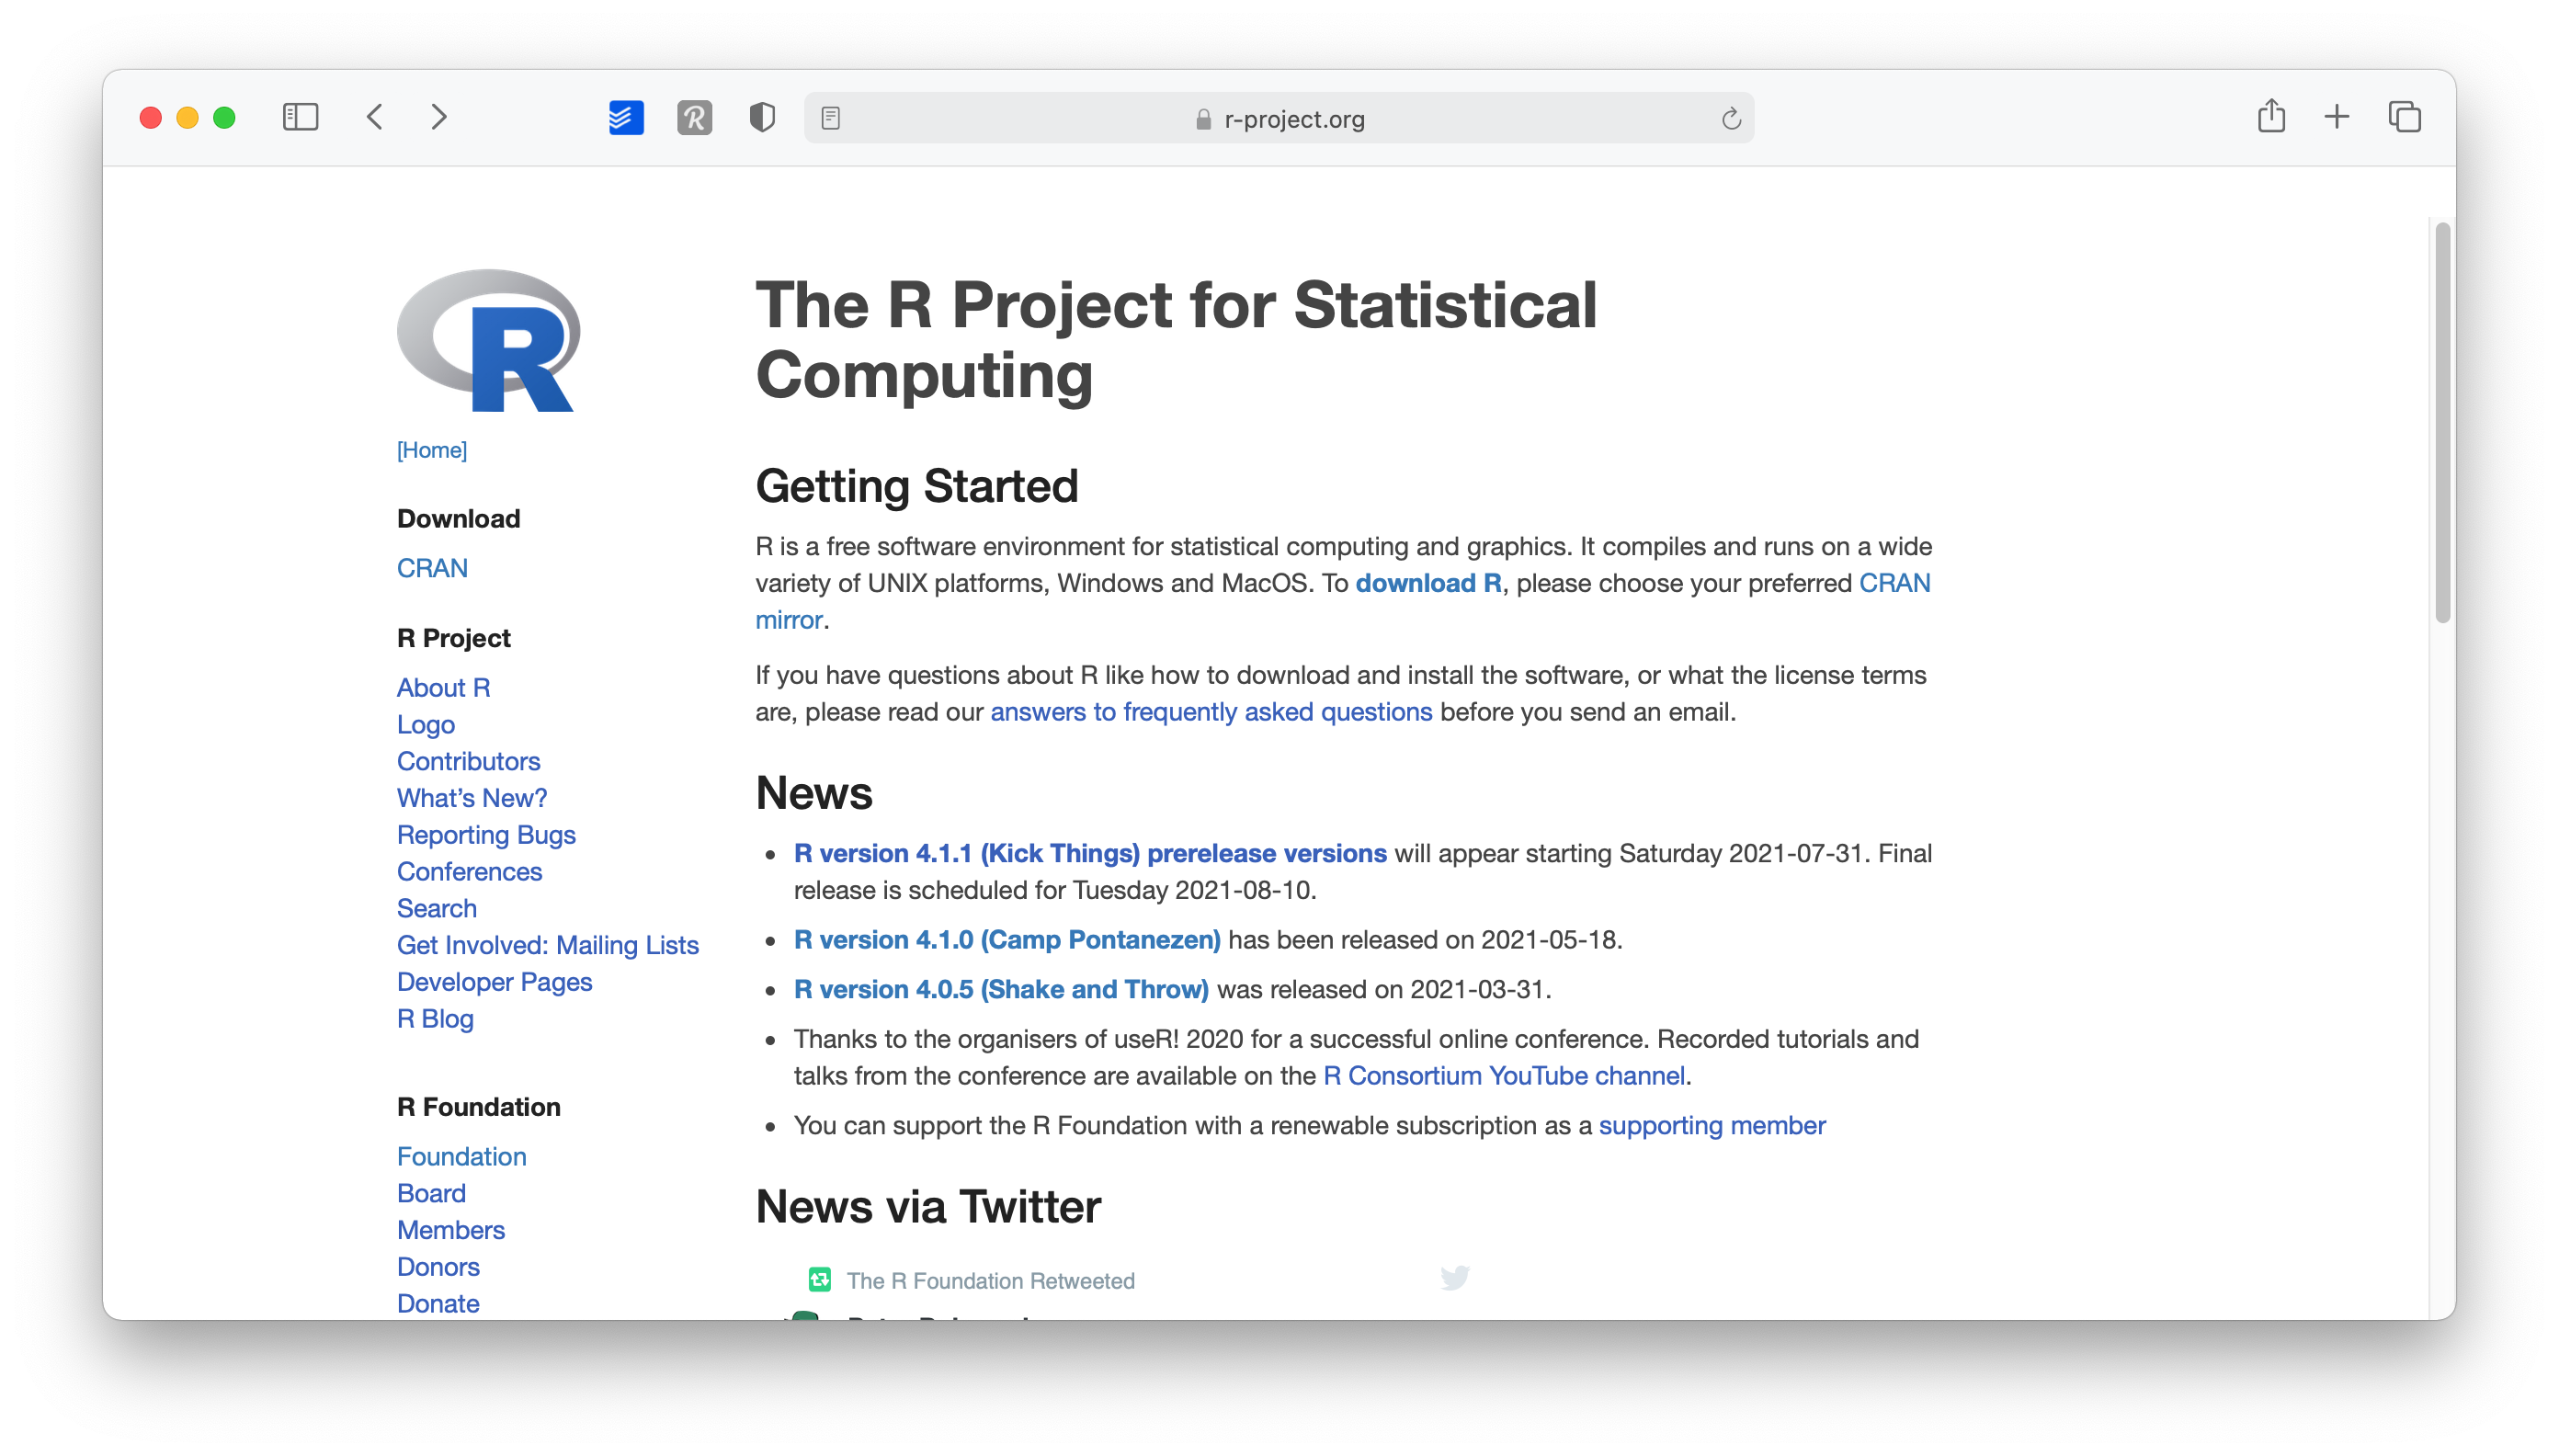
\includegraphics{images/chapter_03_img/r_project/00_r_project_page.png}
\item
  Click on \texttt{CRAN} where it says \texttt{Download}.
\item
  Choose a server in your country (all of them work, but downloads will
  perform quicker if you choose your country or one that is close to
  where you are).

  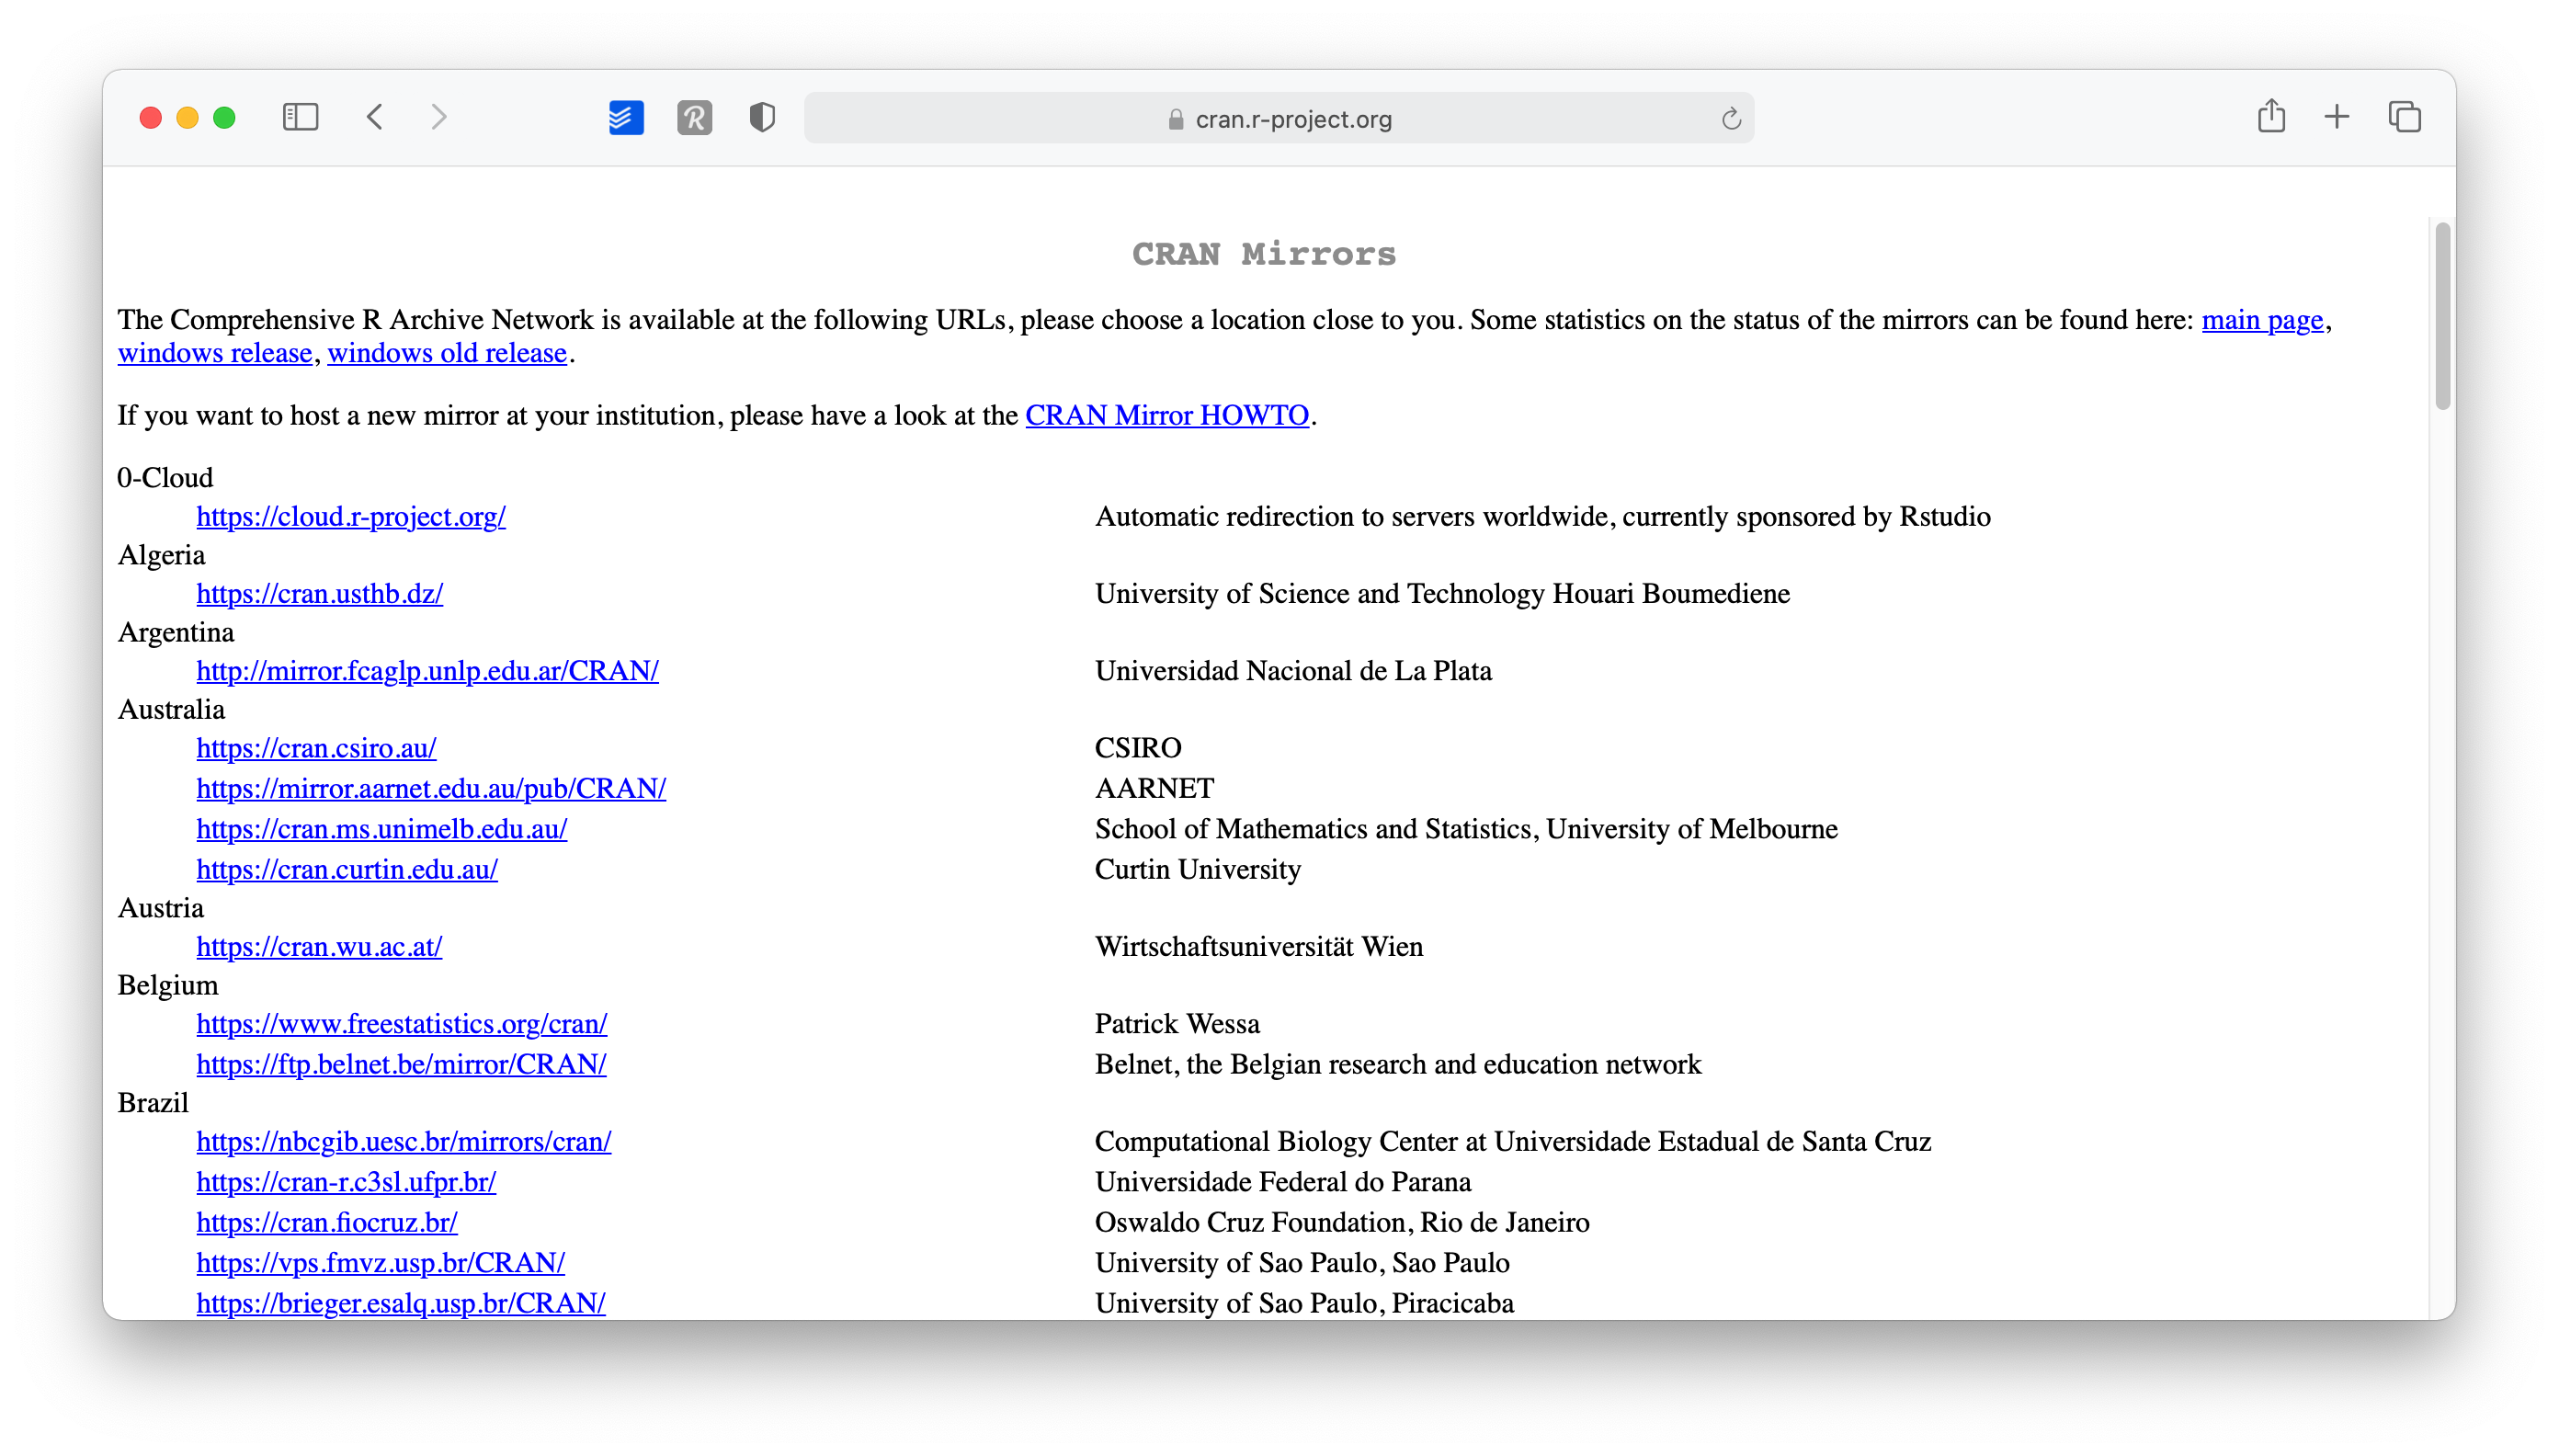
\includegraphics{images/chapter_03_img/r_project/01_r_project_cran_mirror.png}
\item
  Select the operating system for your computer, for example
  \texttt{Download\ R\ for\ macOS}.

  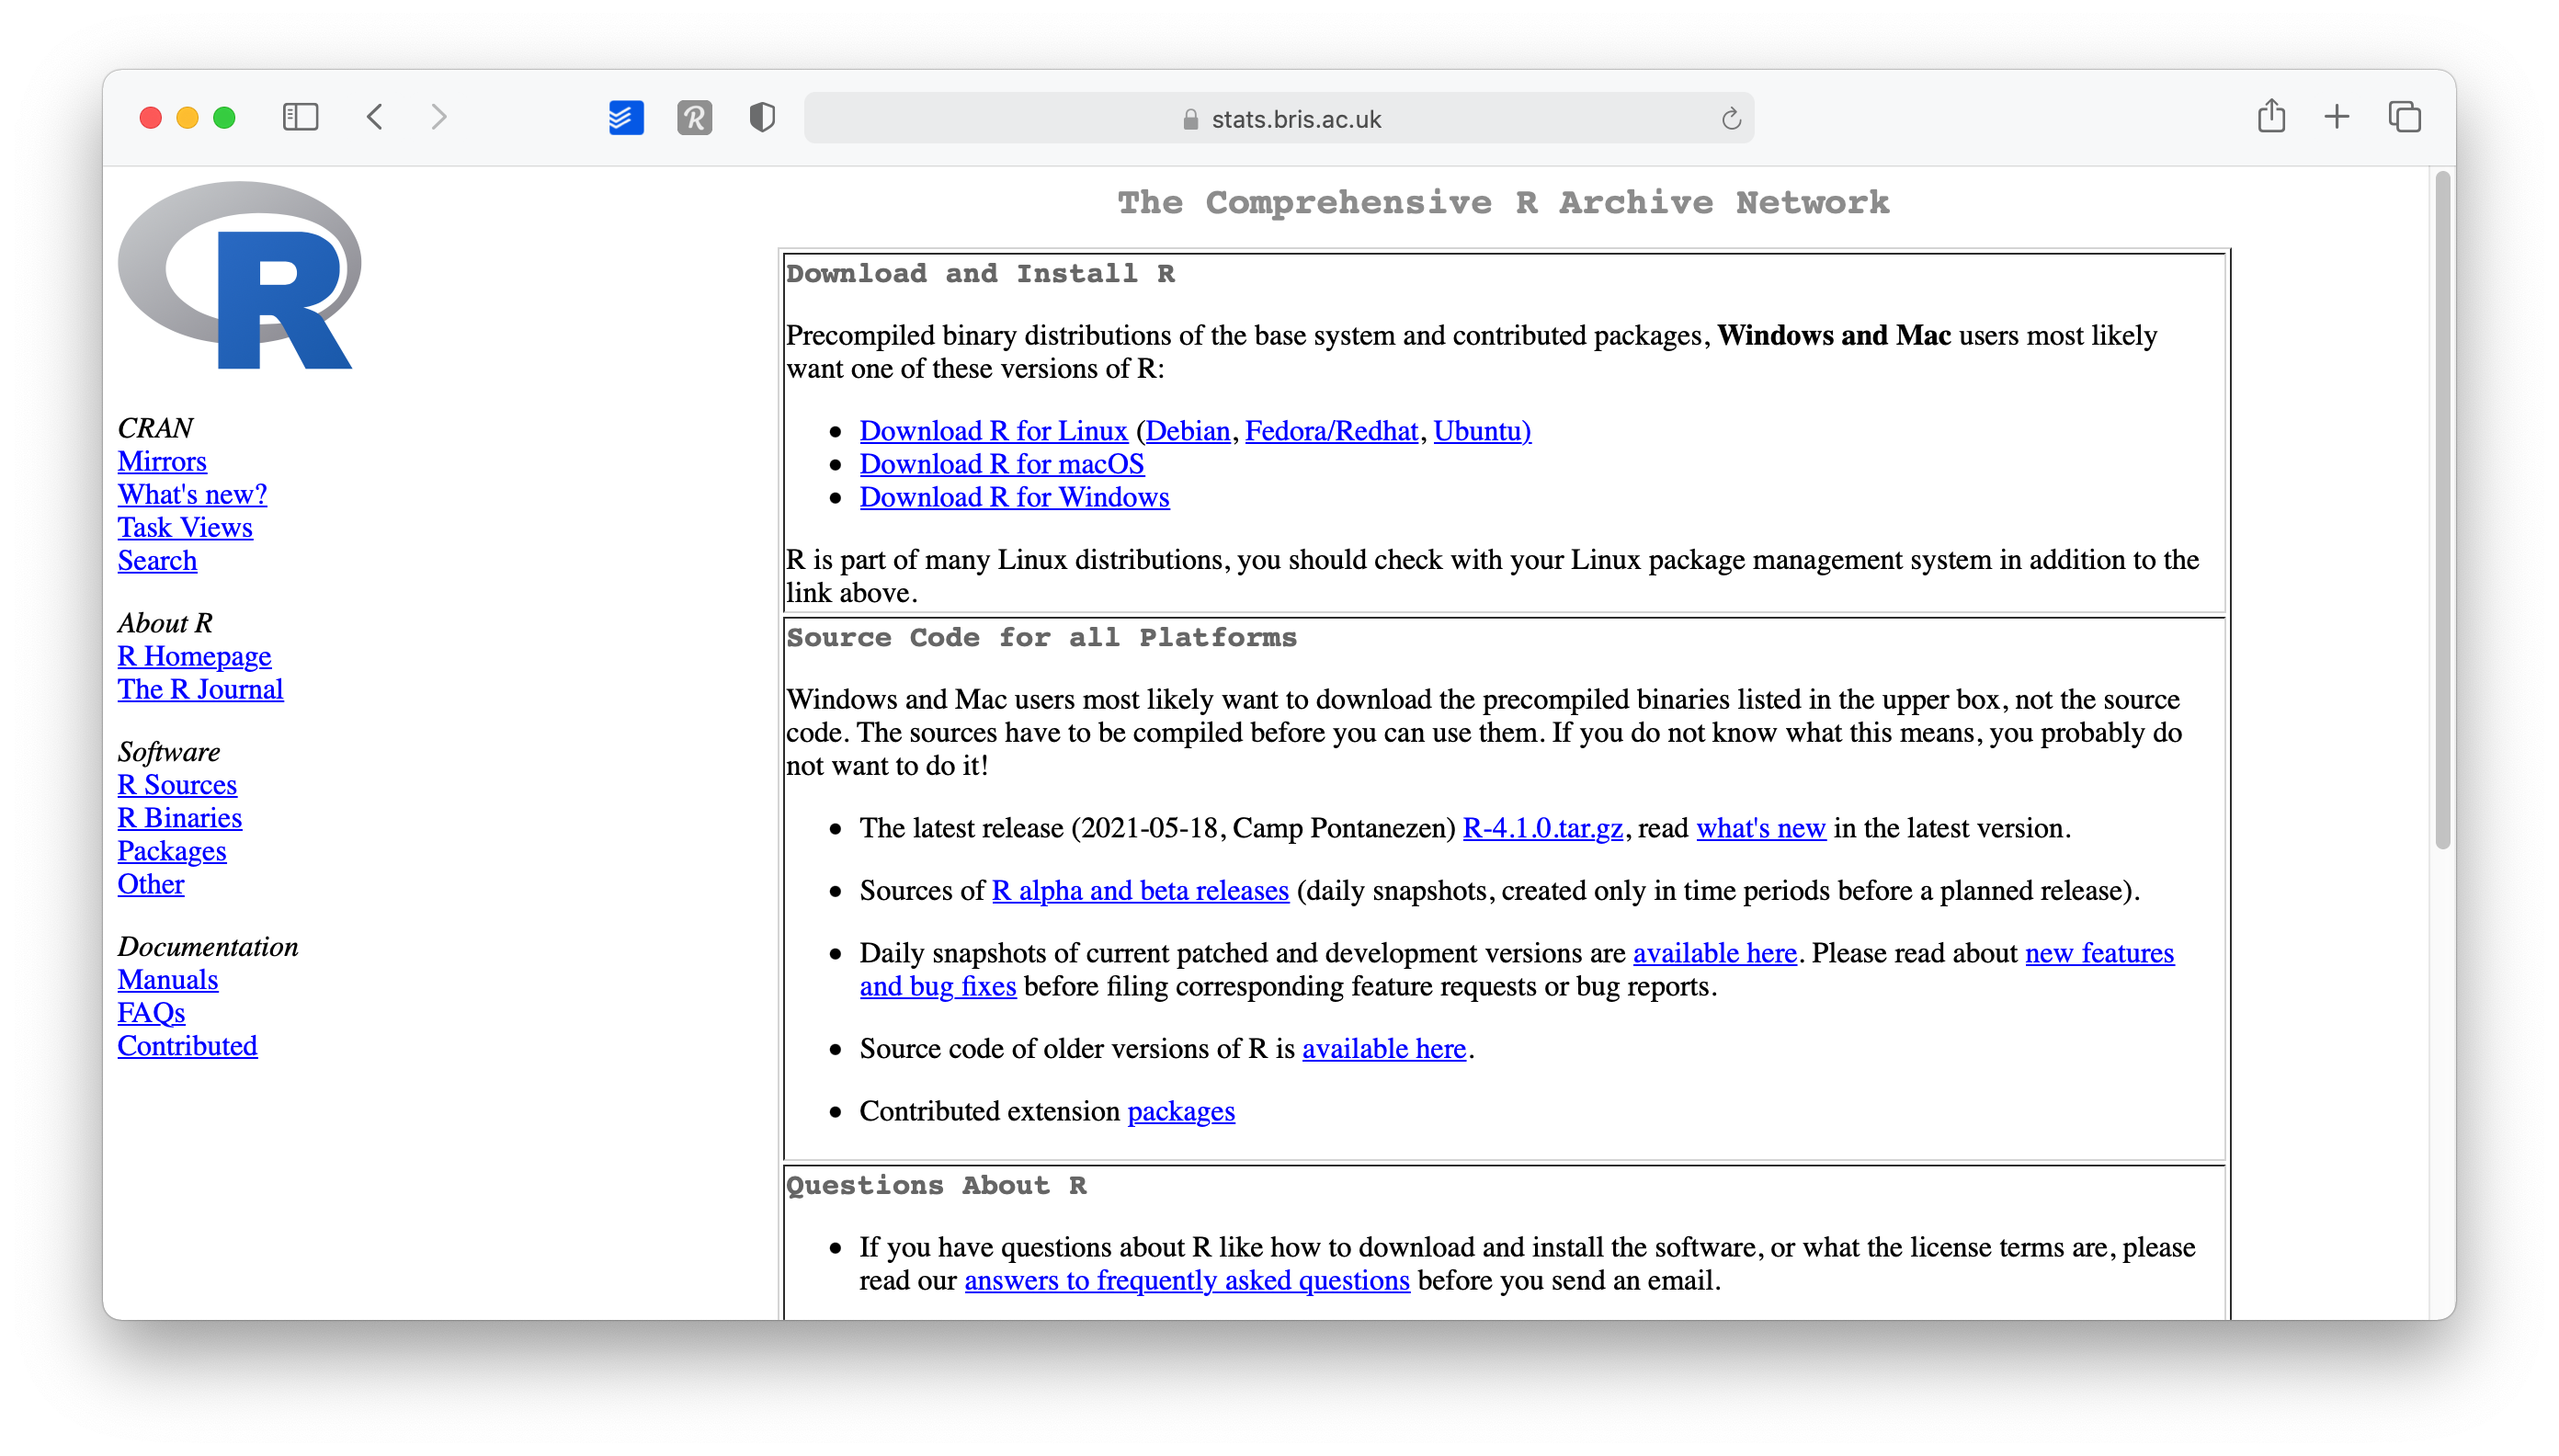
\includegraphics{images/chapter_03_img/r_project/02_r_project_os_choice.png}
\item
  Select the version you want to install (I recommend the latest
  version)

  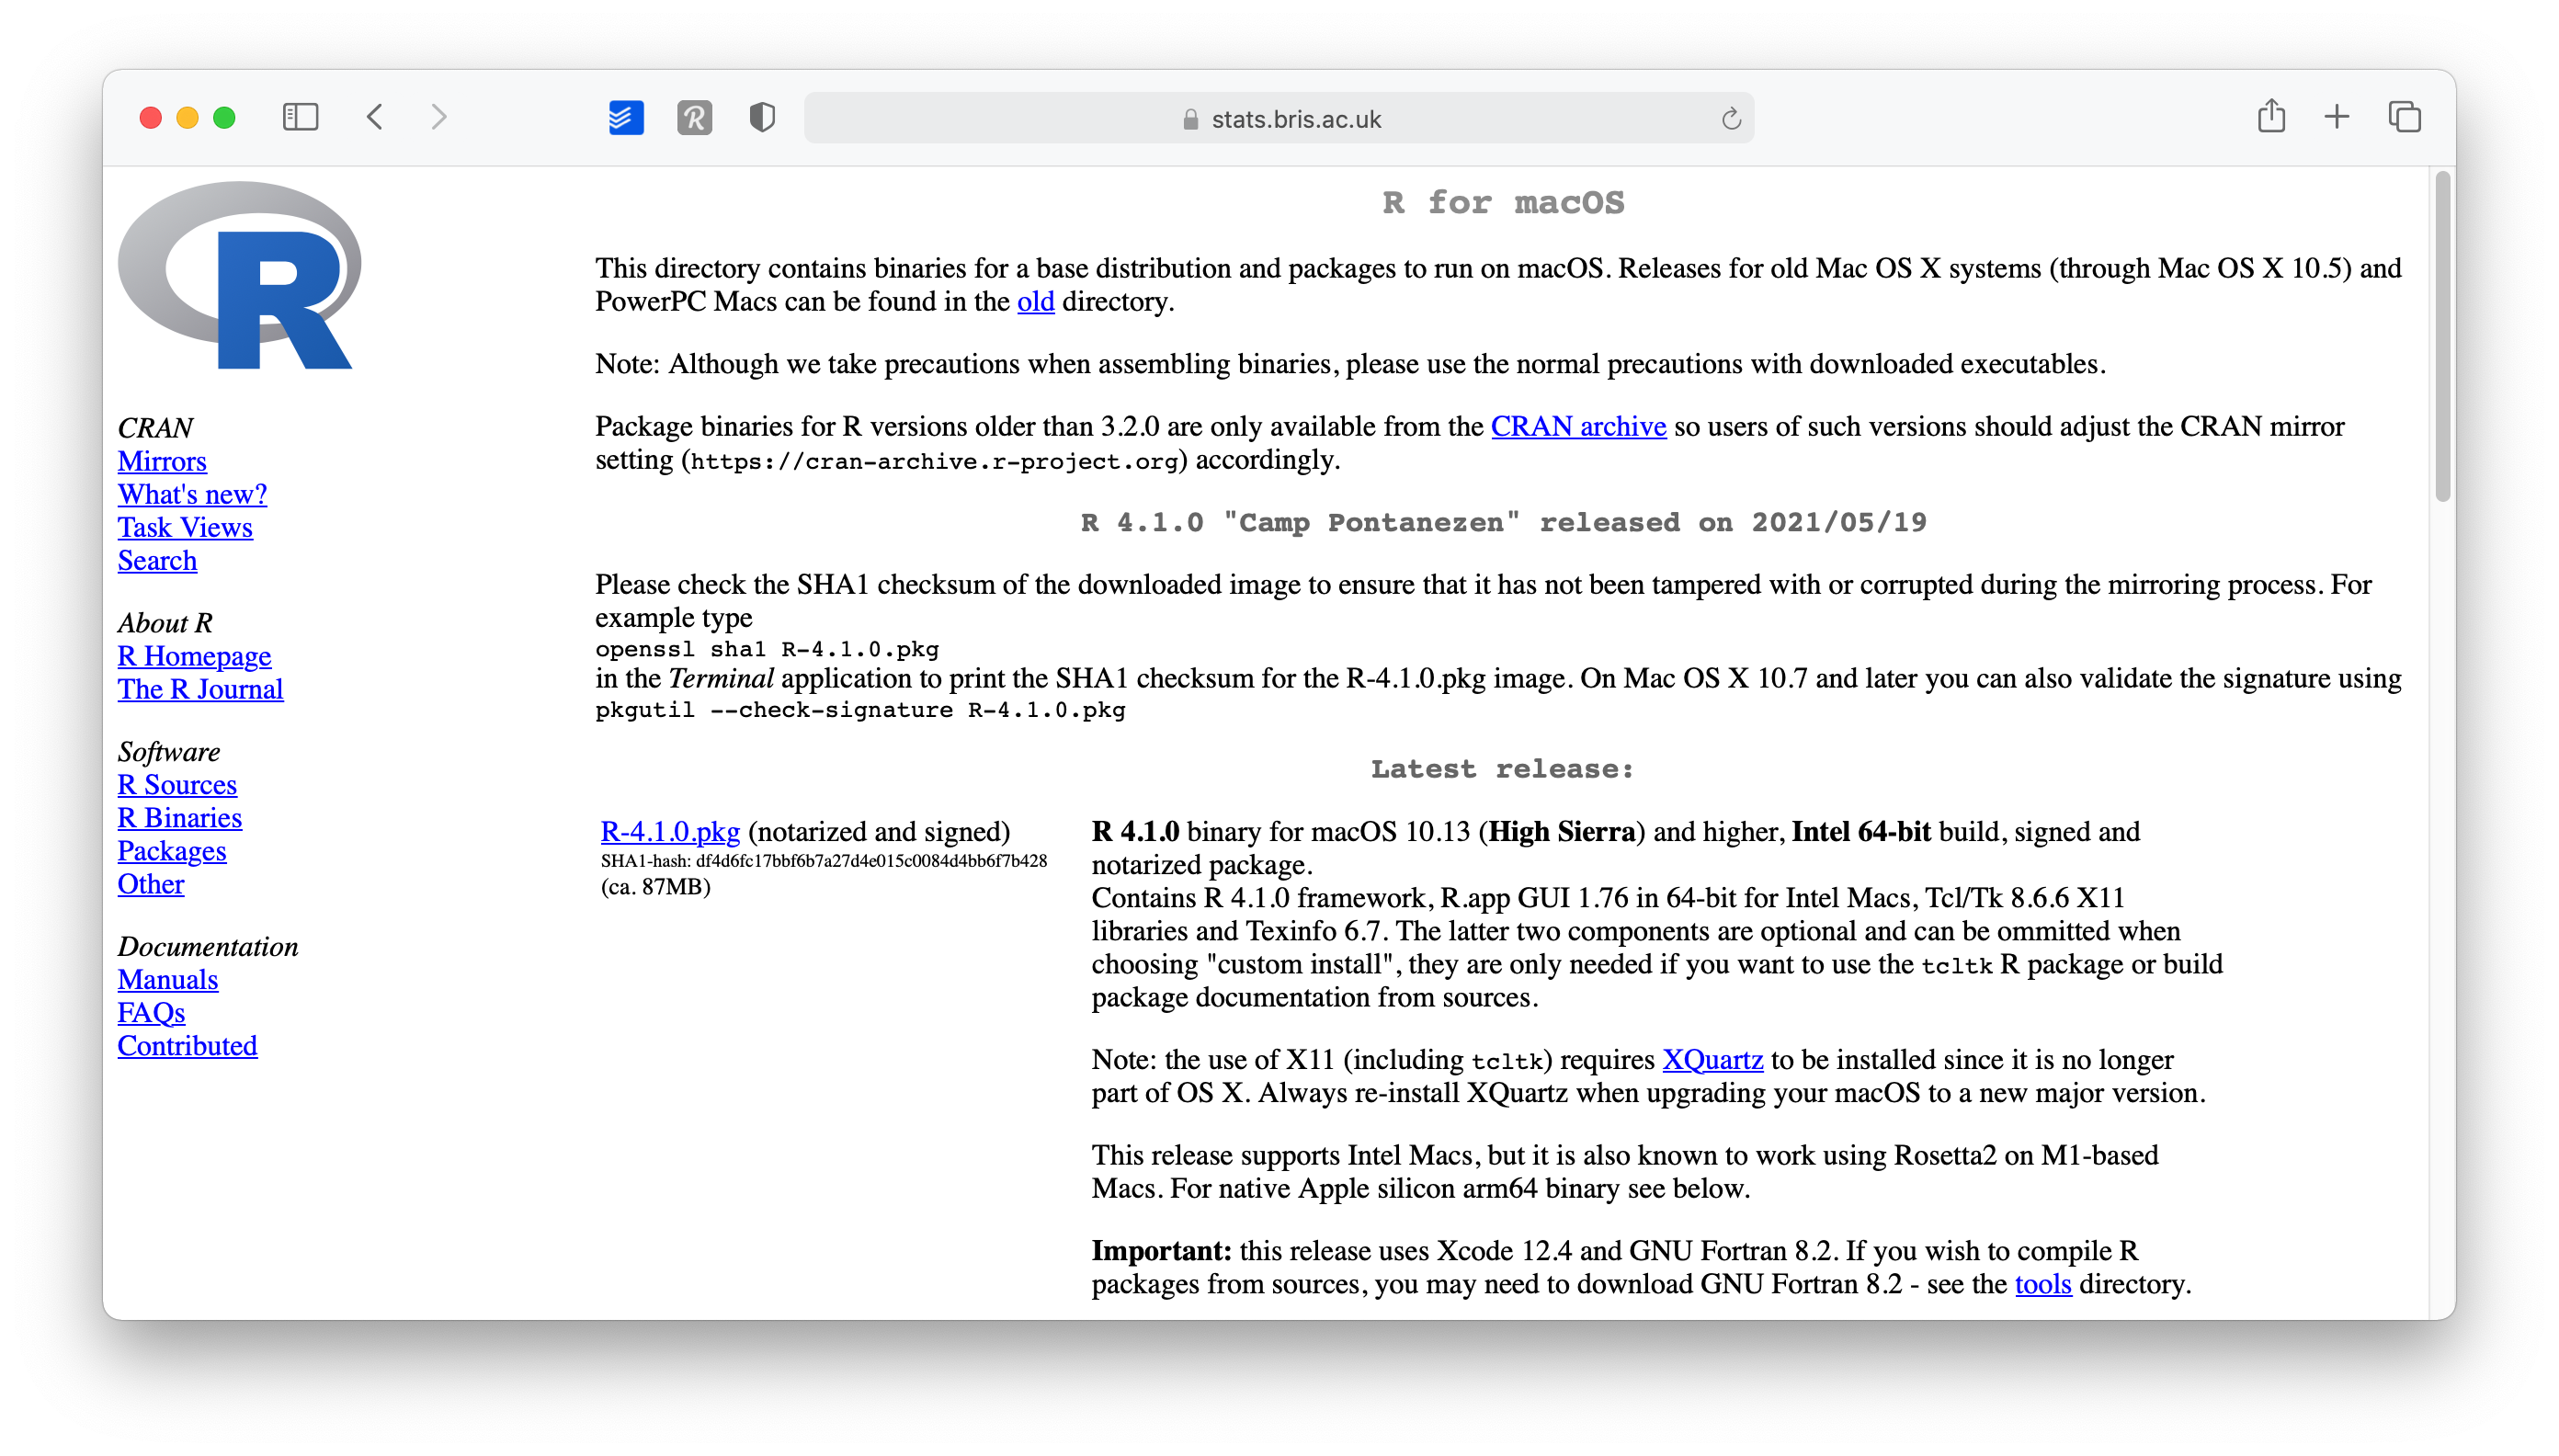
\includegraphics{images/chapter_03_img/r_project/03_r_project_version_choice.png}
\item
  Open the downloaded file and follow the installation instructions. I
  recommend leaving the suggested settings as they are.
\end{enumerate}

This was relatively easy. You now have \emph{R} installed. Technically
you can start using \emph{R} for your research, but there is one more
tool I strongly advise installing: RStudio.

\section{Installing RStudio}\label{installing-rstudio}

\emph{R} by itself is just the `\emph{beating heart}' of \emph{R}
programming, but it has no particular user interface. If you want
buttons to click and actually `\emph{see}' what you are doing, there is
no better way than RStudio. RStudio is an \emph{integrated development
environment} (IDE) and will be our primary tool to interact with
\emph{R}. It is the only software you need to do all the fun parts and,
of course, to follow along with the examples of this book. To install
RStudio perform the following steps:

\begin{enumerate}
\def\labelenumi{\arabic{enumi}.}
\item
  Go to \url{http://posit.co} and click on \texttt{DOWNLOAD\ RSTUDIO}.

  
\includegraphics{images/chapter_03_img/rstudio/01_posit_main_page.png}
\item
  Click on \texttt{DOWNLOAD\ RSTUDIO} on this page.

  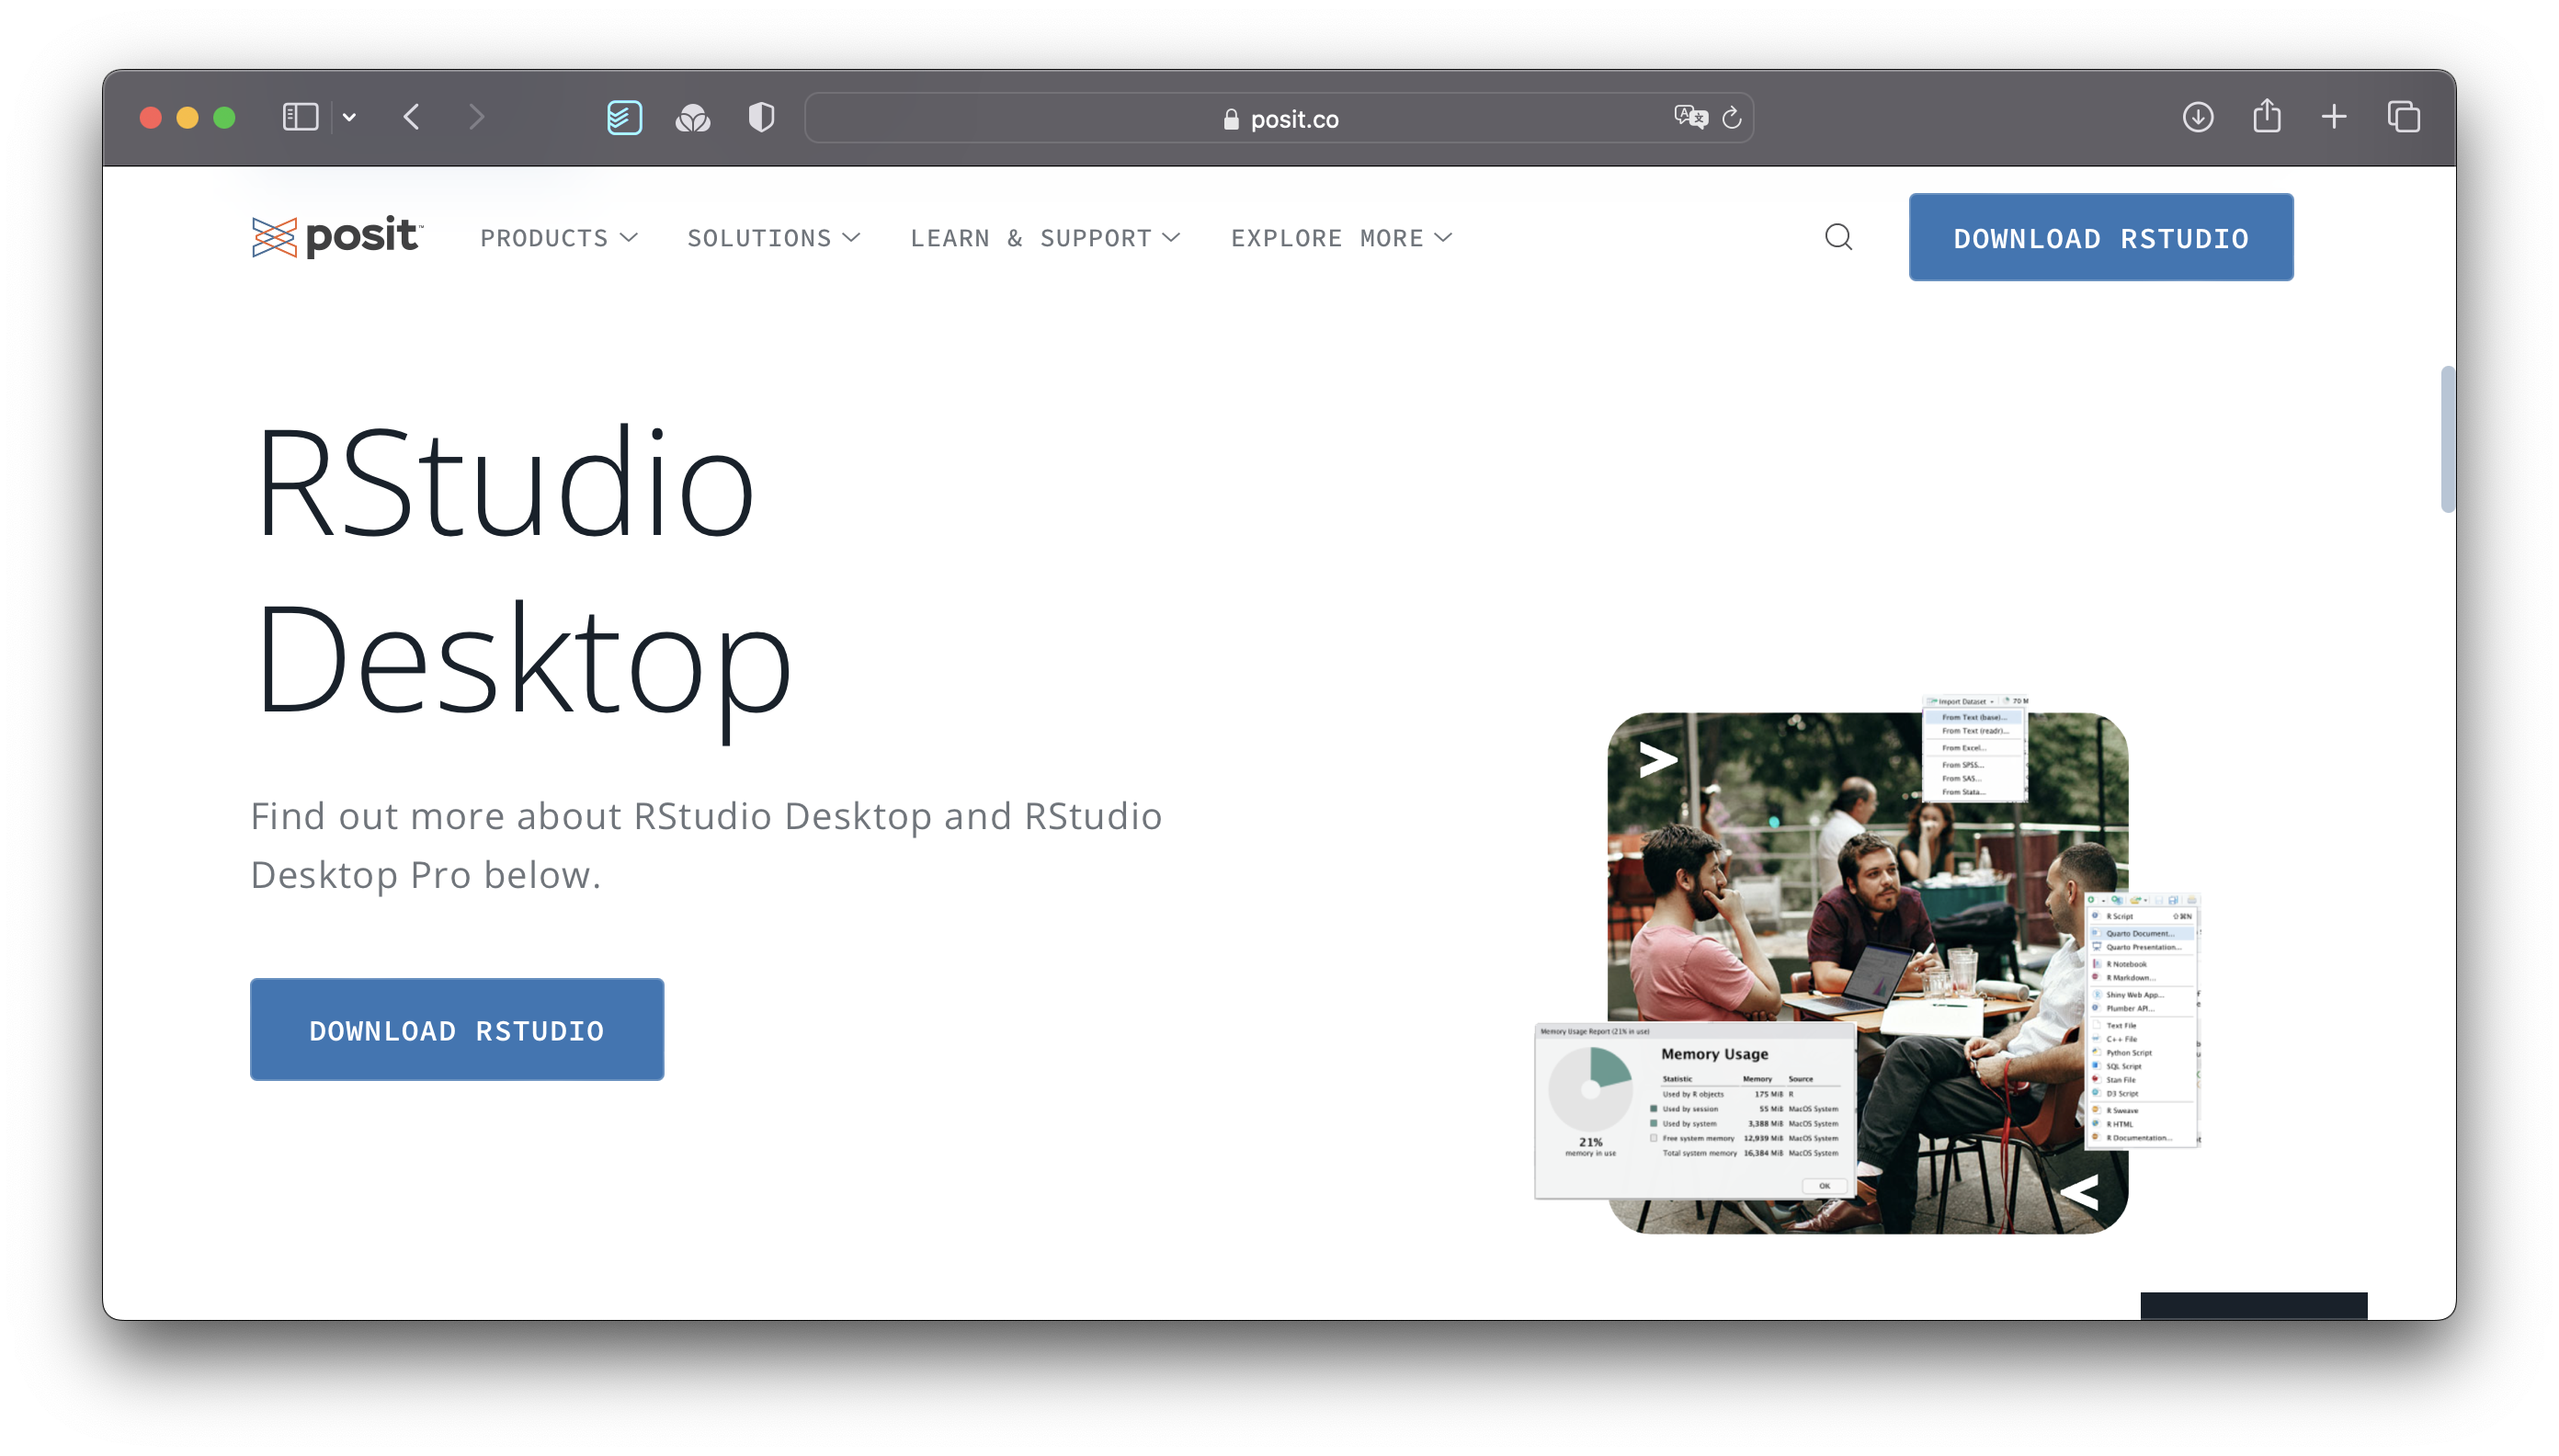
\includegraphics{images/chapter_03_img/rstudio/02_posit_rstudio_desktop.png}
\item
  This leads you to the page where you can install \emph{R} as a first
  step and RStudio as a second step. Since we installed \emph{R}
  already, we can click on
  \texttt{DOWNLOAD\ RSTUDIO\ DESKTOP\ FOR\ WINDOWS} (or for Mac if you
  are not using a PC).

  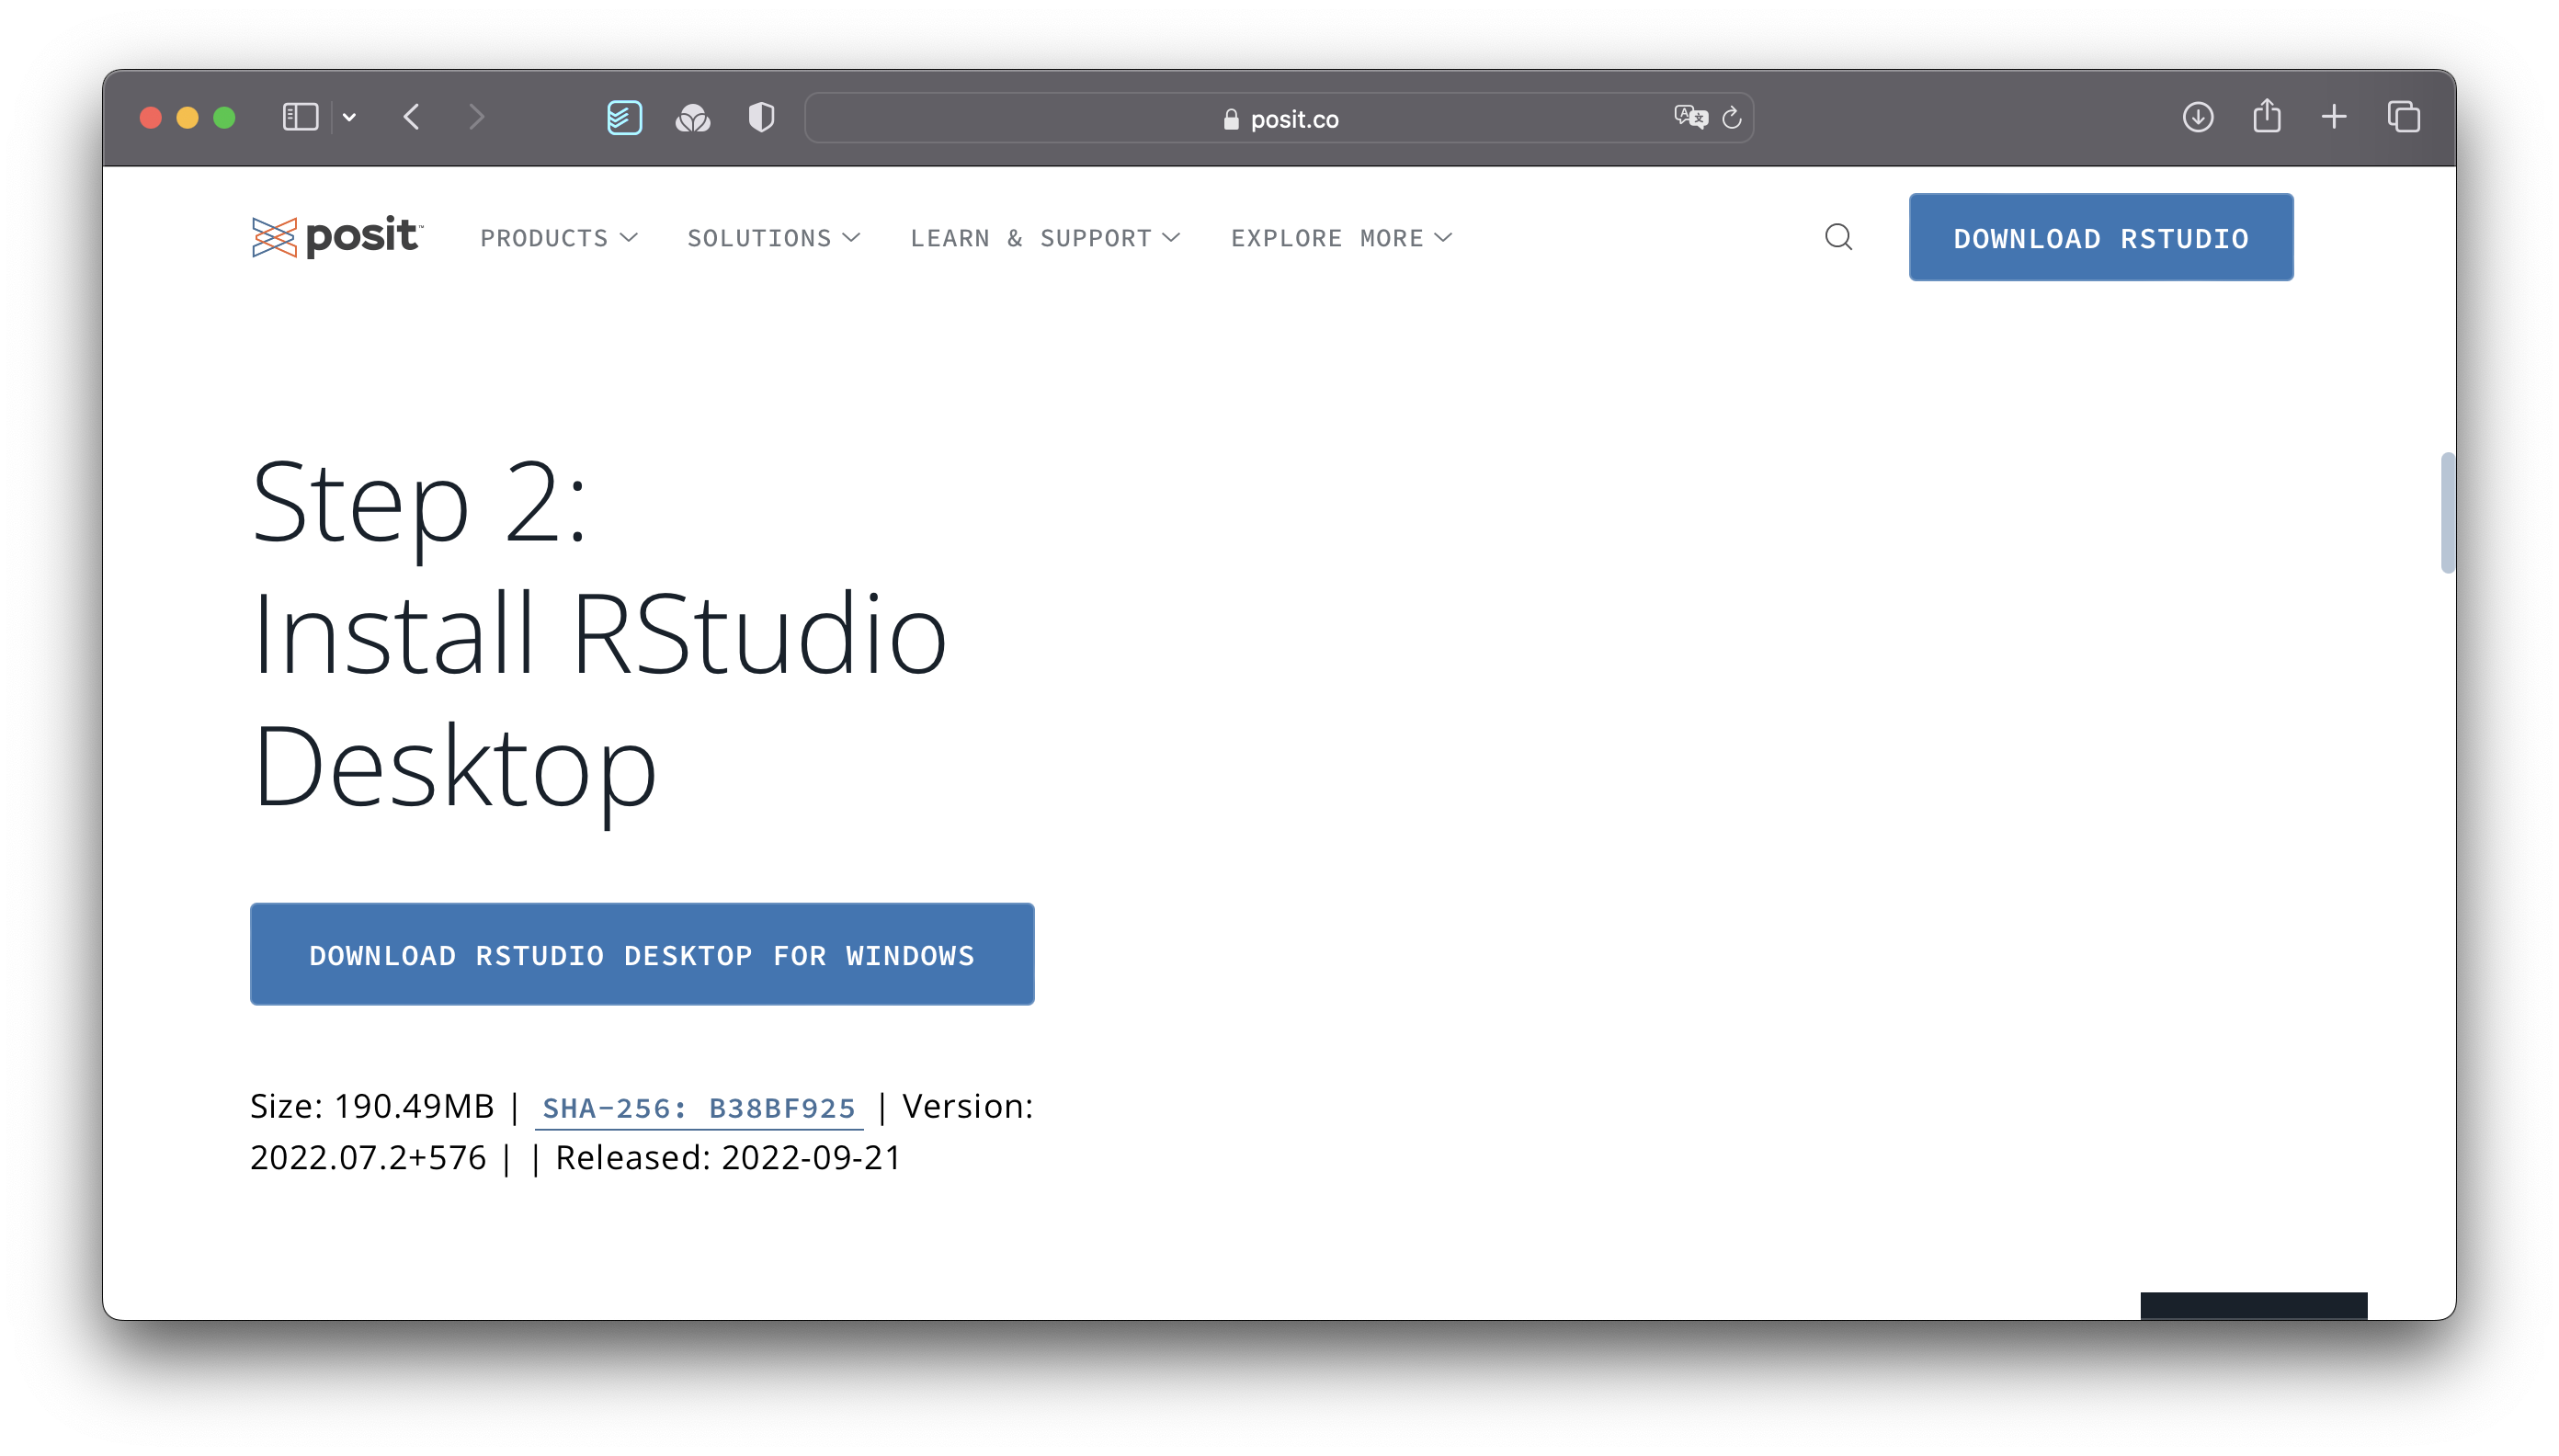
\includegraphics{images/chapter_03_img/rstudio/03_posit_installer.png}
\item
  If for some reason the version for your operating system is not
  showing up correctly, you can scroll down and find other version ready
  to be installed.

  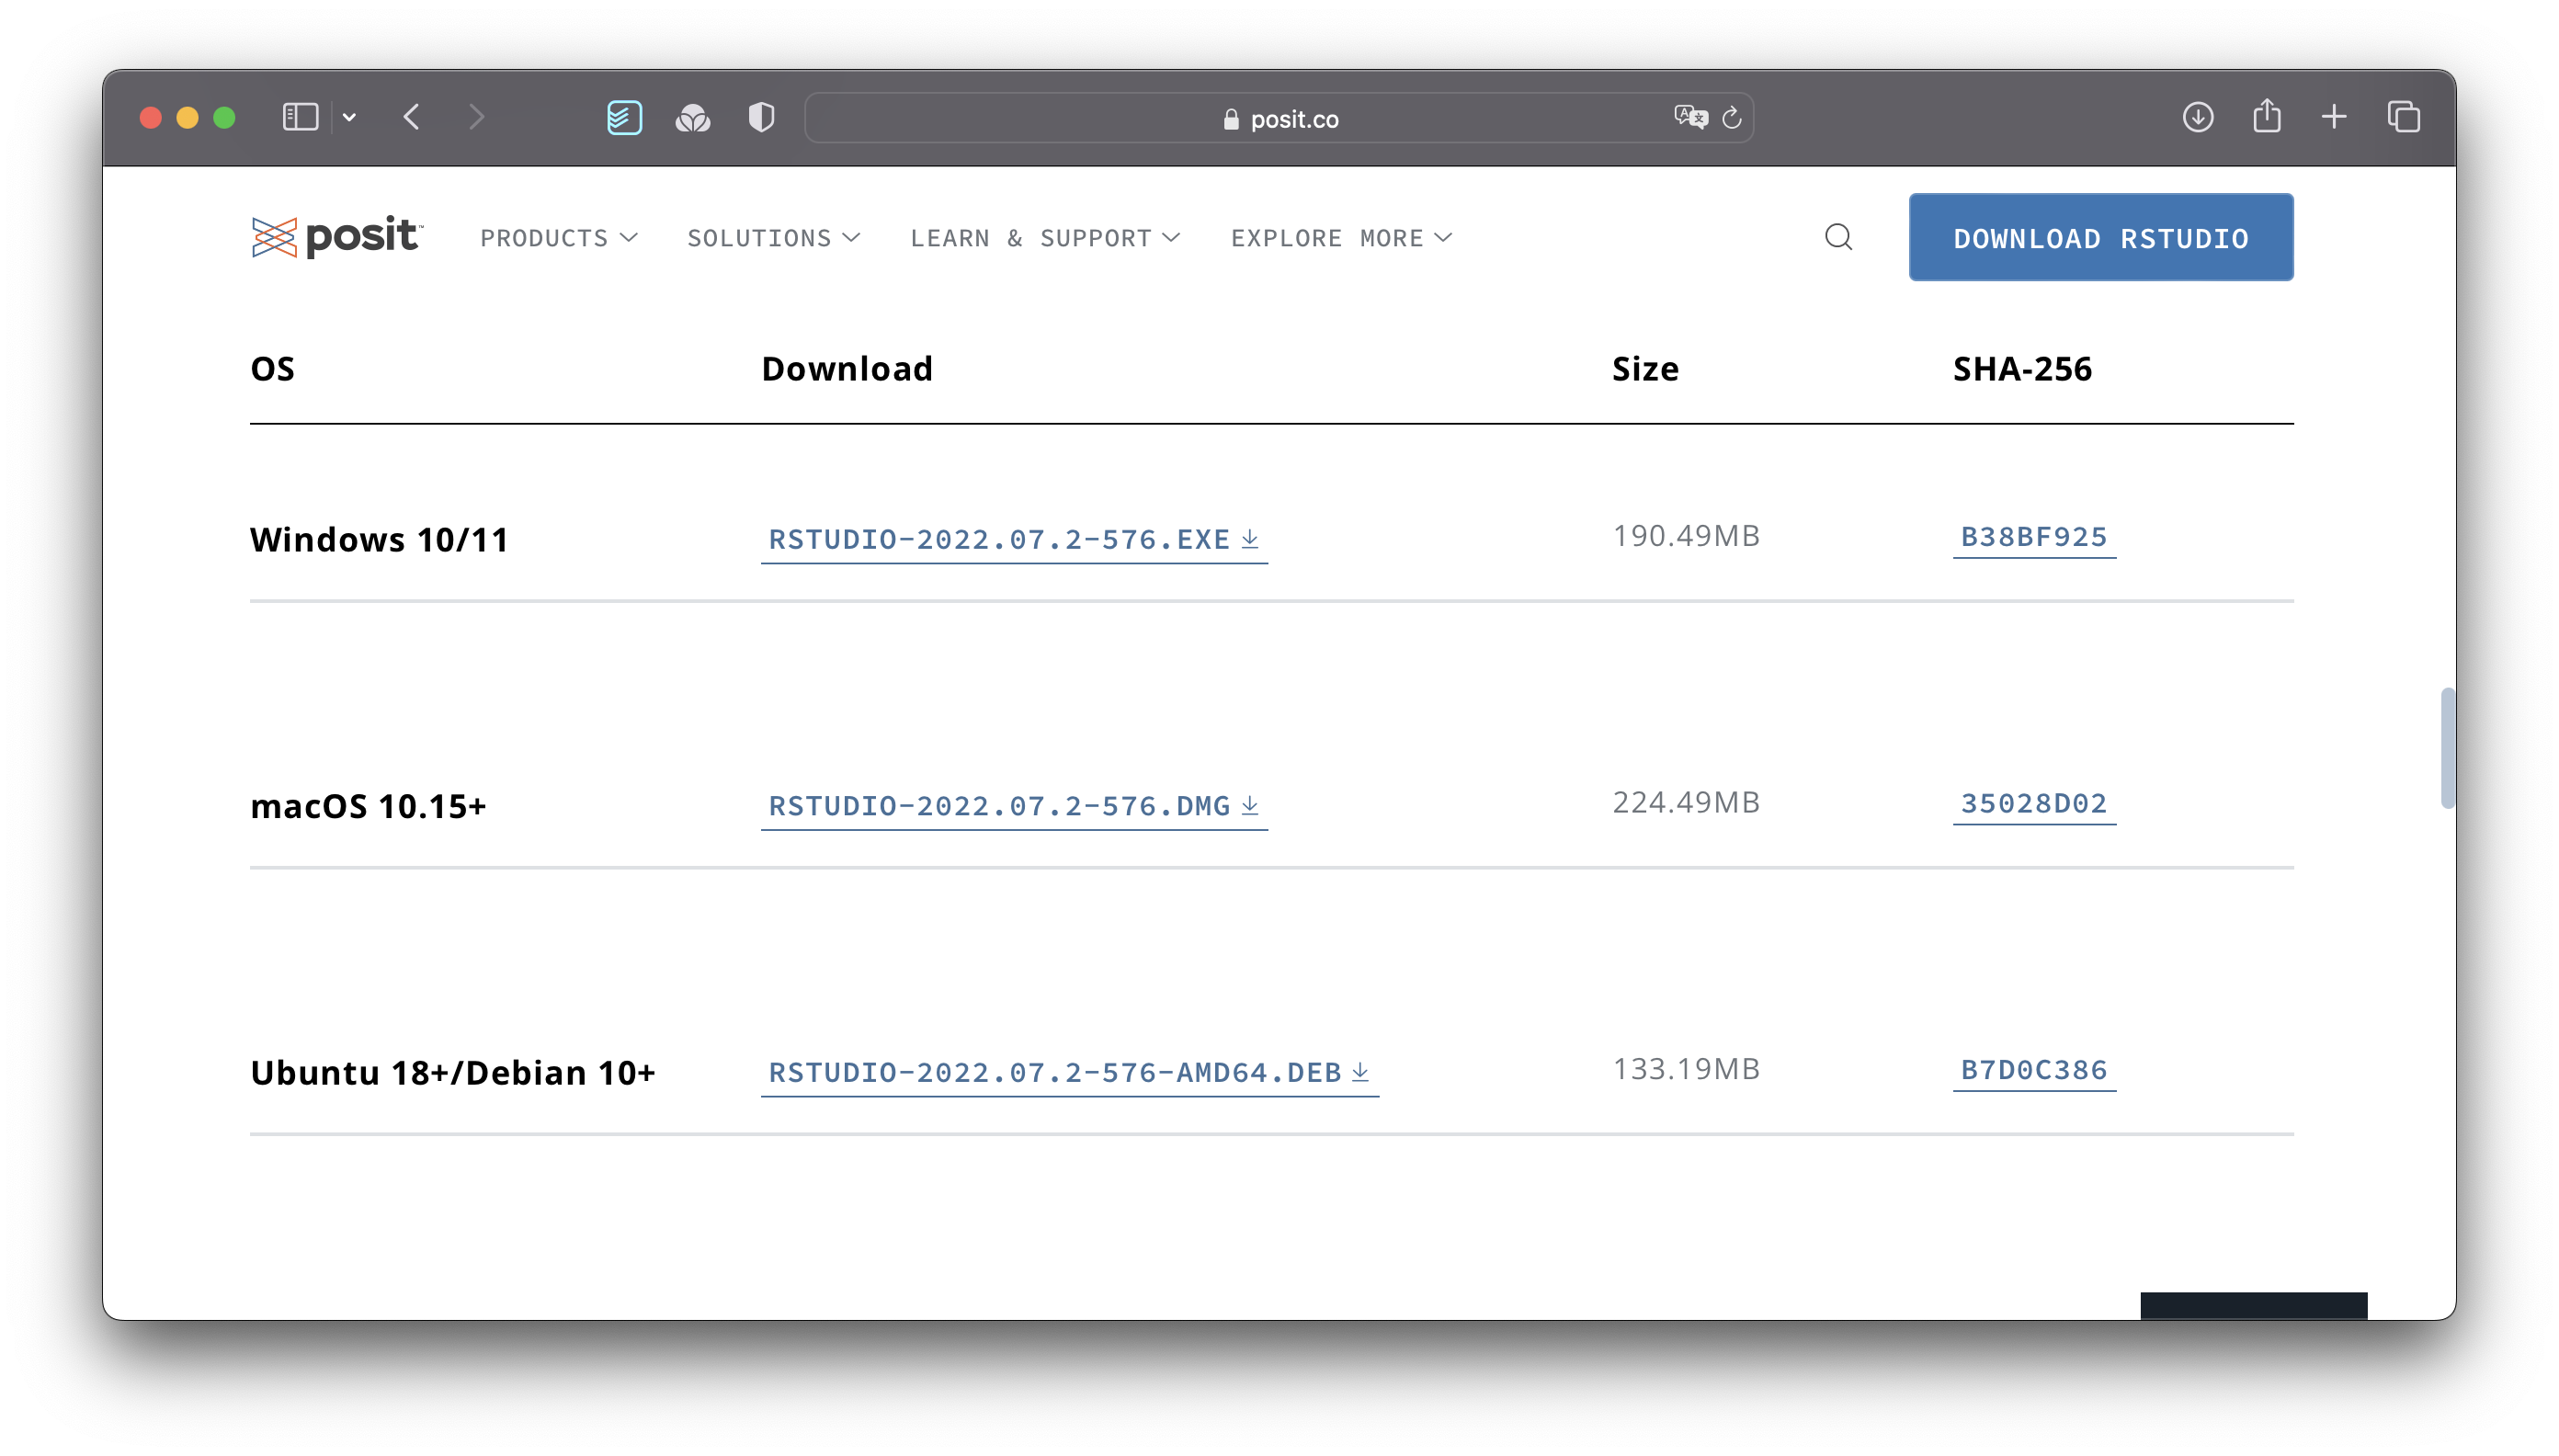
\includegraphics{images/chapter_03_img/rstudio/04_other_installers.png}
\item
  Open the downloaded file and follow the installation instructions.
  Again, keep it to the default settings as much as possible.
\end{enumerate}

Congratulations, you are all set up to learn \emph{R}. From now on you
only need to start RStudio and not \emph{R}. Of course, if you are the
curious type, nothing shall stop you to try \emph{R} without RStudio.

\section{When you first start
RStudio}\label{when-you-first-start-rstudio}

Before you start programming away, you might want to make some tweaks to
your settings right away to have a better experience (in my humble
opinion). To open the Rstudio settings you have to click on

\begin{itemize}
\item
  \texttt{RStudio\ \textgreater{}\ Tools\ \textgreater{}\ Global\ Options}
  or press \texttt{⌘\ +\ ,} if you are on a Mac.
\item
  \texttt{RStudio\ \textgreater{}\ Tools\ \textgreater{}\ Global\ Options}
  or press \texttt{Ctrl\ +\ ,} if you work on a Windows computer.
\end{itemize}

I recommend to at least make the following changes to set yourself up
for success right from the beginning:

\begin{enumerate}
\def\labelenumi{\arabic{enumi}.}
\item
  Already on the first tab,
  i.e.~\texttt{General\ \textgreater{}\ Basic}, we should make one of
  the most significant changes. Deactivate every option that starts with
  \texttt{Restore}. This will ensure that every time you start RStudio,
  you begin with a clean slate. At first sight, it might sound
  counter-intuitive not to restart everything where you left off, but it
  is essential to make all your projects easily reproducible.
  Furthermore, if you work together with others, not restoring your
  personal settings also ensures that your programming works across
  different computers. Therefore, I recommend having the following
  unticked:

  \begin{itemize}
  \item
    \texttt{Restore\ most\ recently\ opened\ project\ at\ startup},
  \item
    \texttt{Restore\ previsouly\ open\ source\ documents\ at\ startup},
  \item
    \texttt{Restore\ .Rdata\ into\ workspace\ at\ startup}

    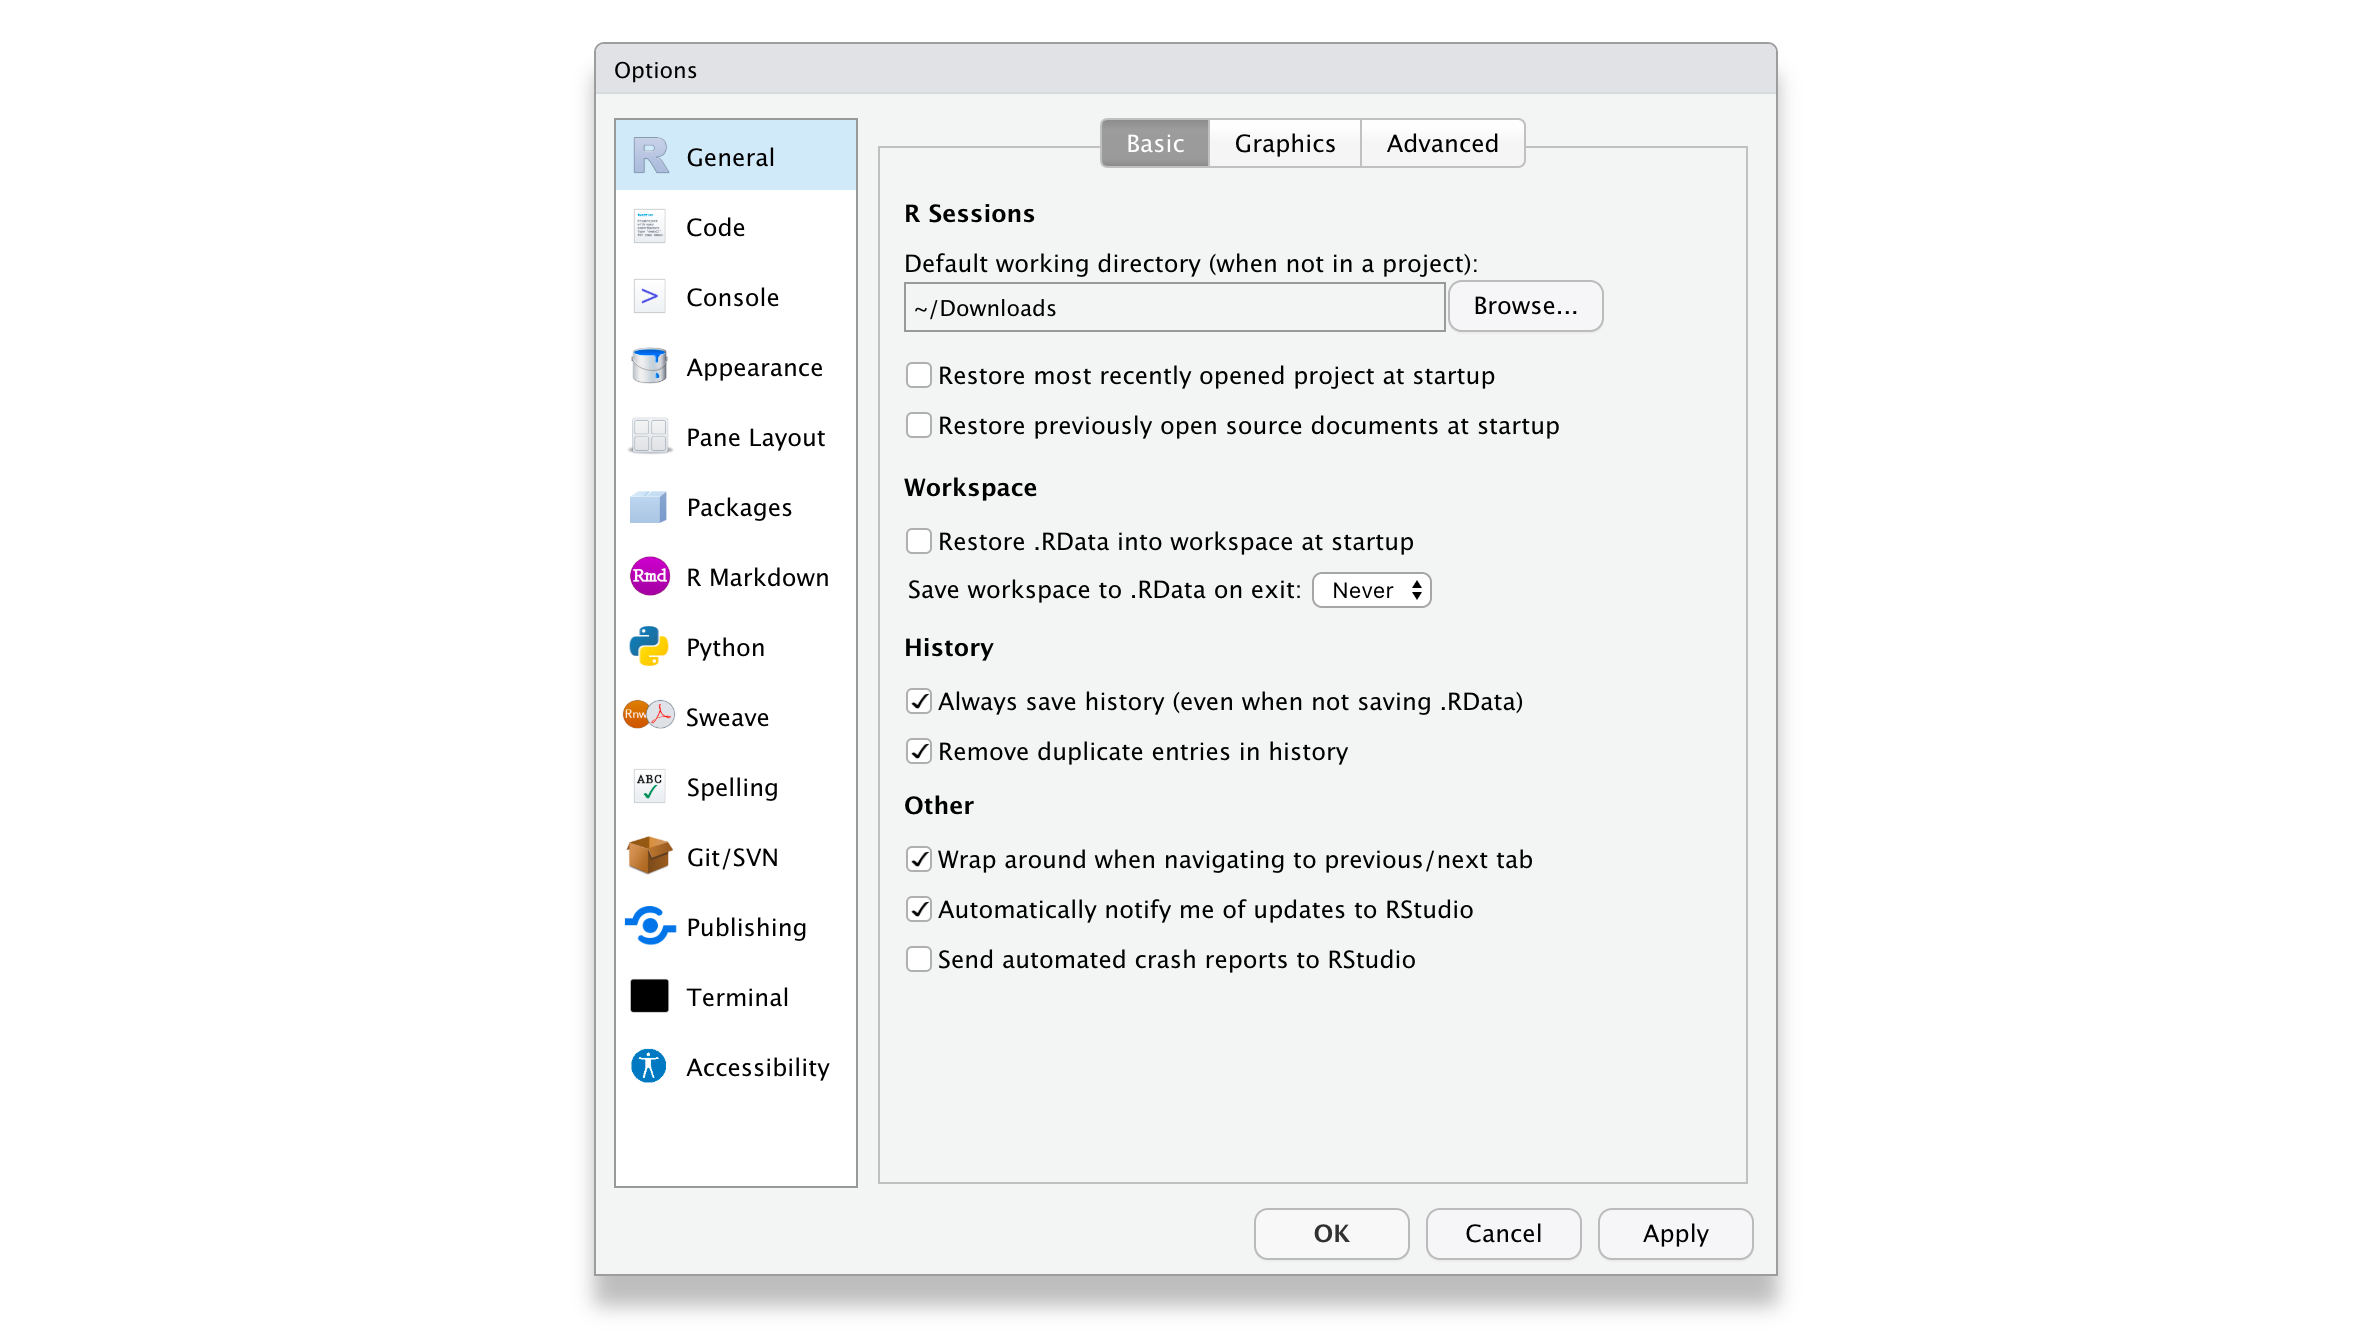
\includegraphics{images/chapter_03_img/rstudio_preferences/00_rstudio_preferences_basic.png}
  \end{itemize}
\item
  In the same tab under \texttt{Workspace}, select \texttt{Never} for
  the setting \texttt{Save\ workspace\ to\ .RData\ on\ exit}. One might
  think it is wise to keep intermediary results stored from one R
  session to another. However, I often found myself fixing issues due to
  this lazy method, and my code became less reliable and, therefore,
  reproducible. With experience, you will find that this avoids many
  headaches.
\item
  In the \texttt{Code\ \textgreater{}\ Editing} tab, make sure to have
  at least the first five options ticked, especially the
  \texttt{Auto-indent\ code\ after\ paste}. This setting will save time
  when trying to format your coding appropriately, making it easier to
  read. Indentation is the primary way of making your code look more
  readable and less like a series of characters that appear almost
  random.

  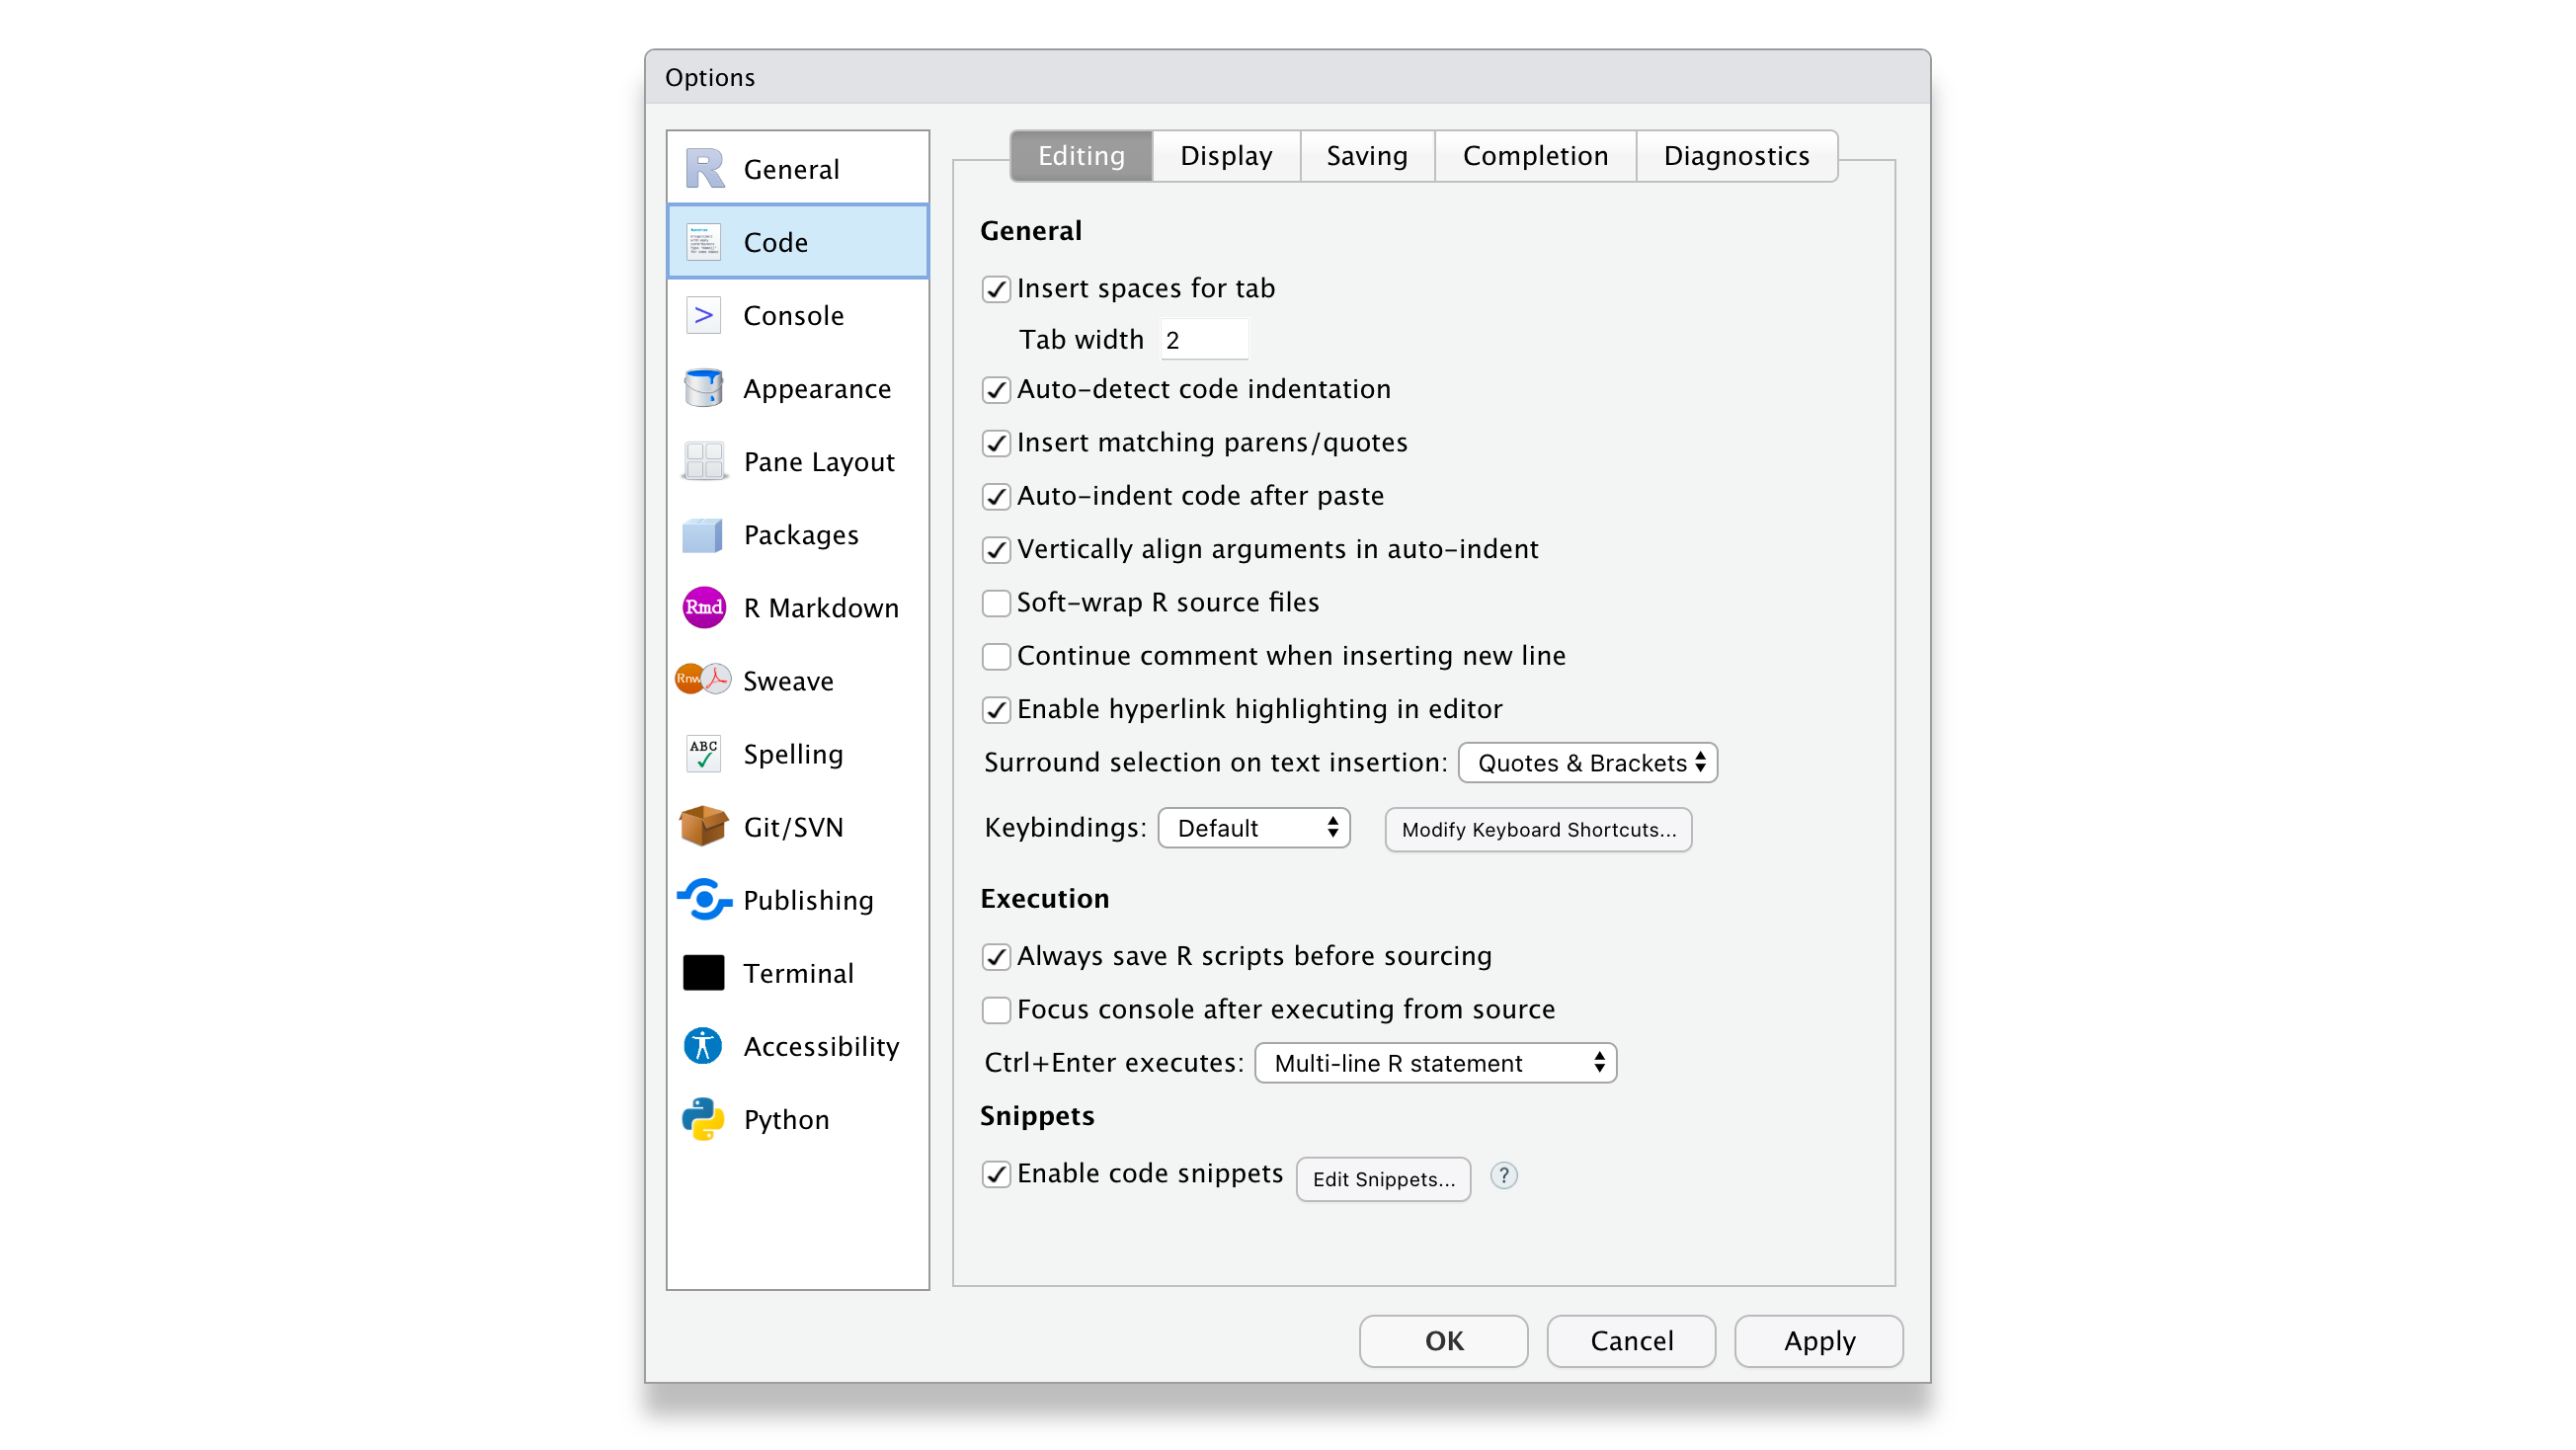
\includegraphics{images/chapter_03_img/rstudio_preferences/01_rstudio_preferences_editing.png}
\item
  In the \texttt{Display} tab, you might want to have the first three
  options selected. In particular, \texttt{Highlight\ selected\ line} is
  helpful because, in more complicated code, it is helpful to see where
  your cursor is.

  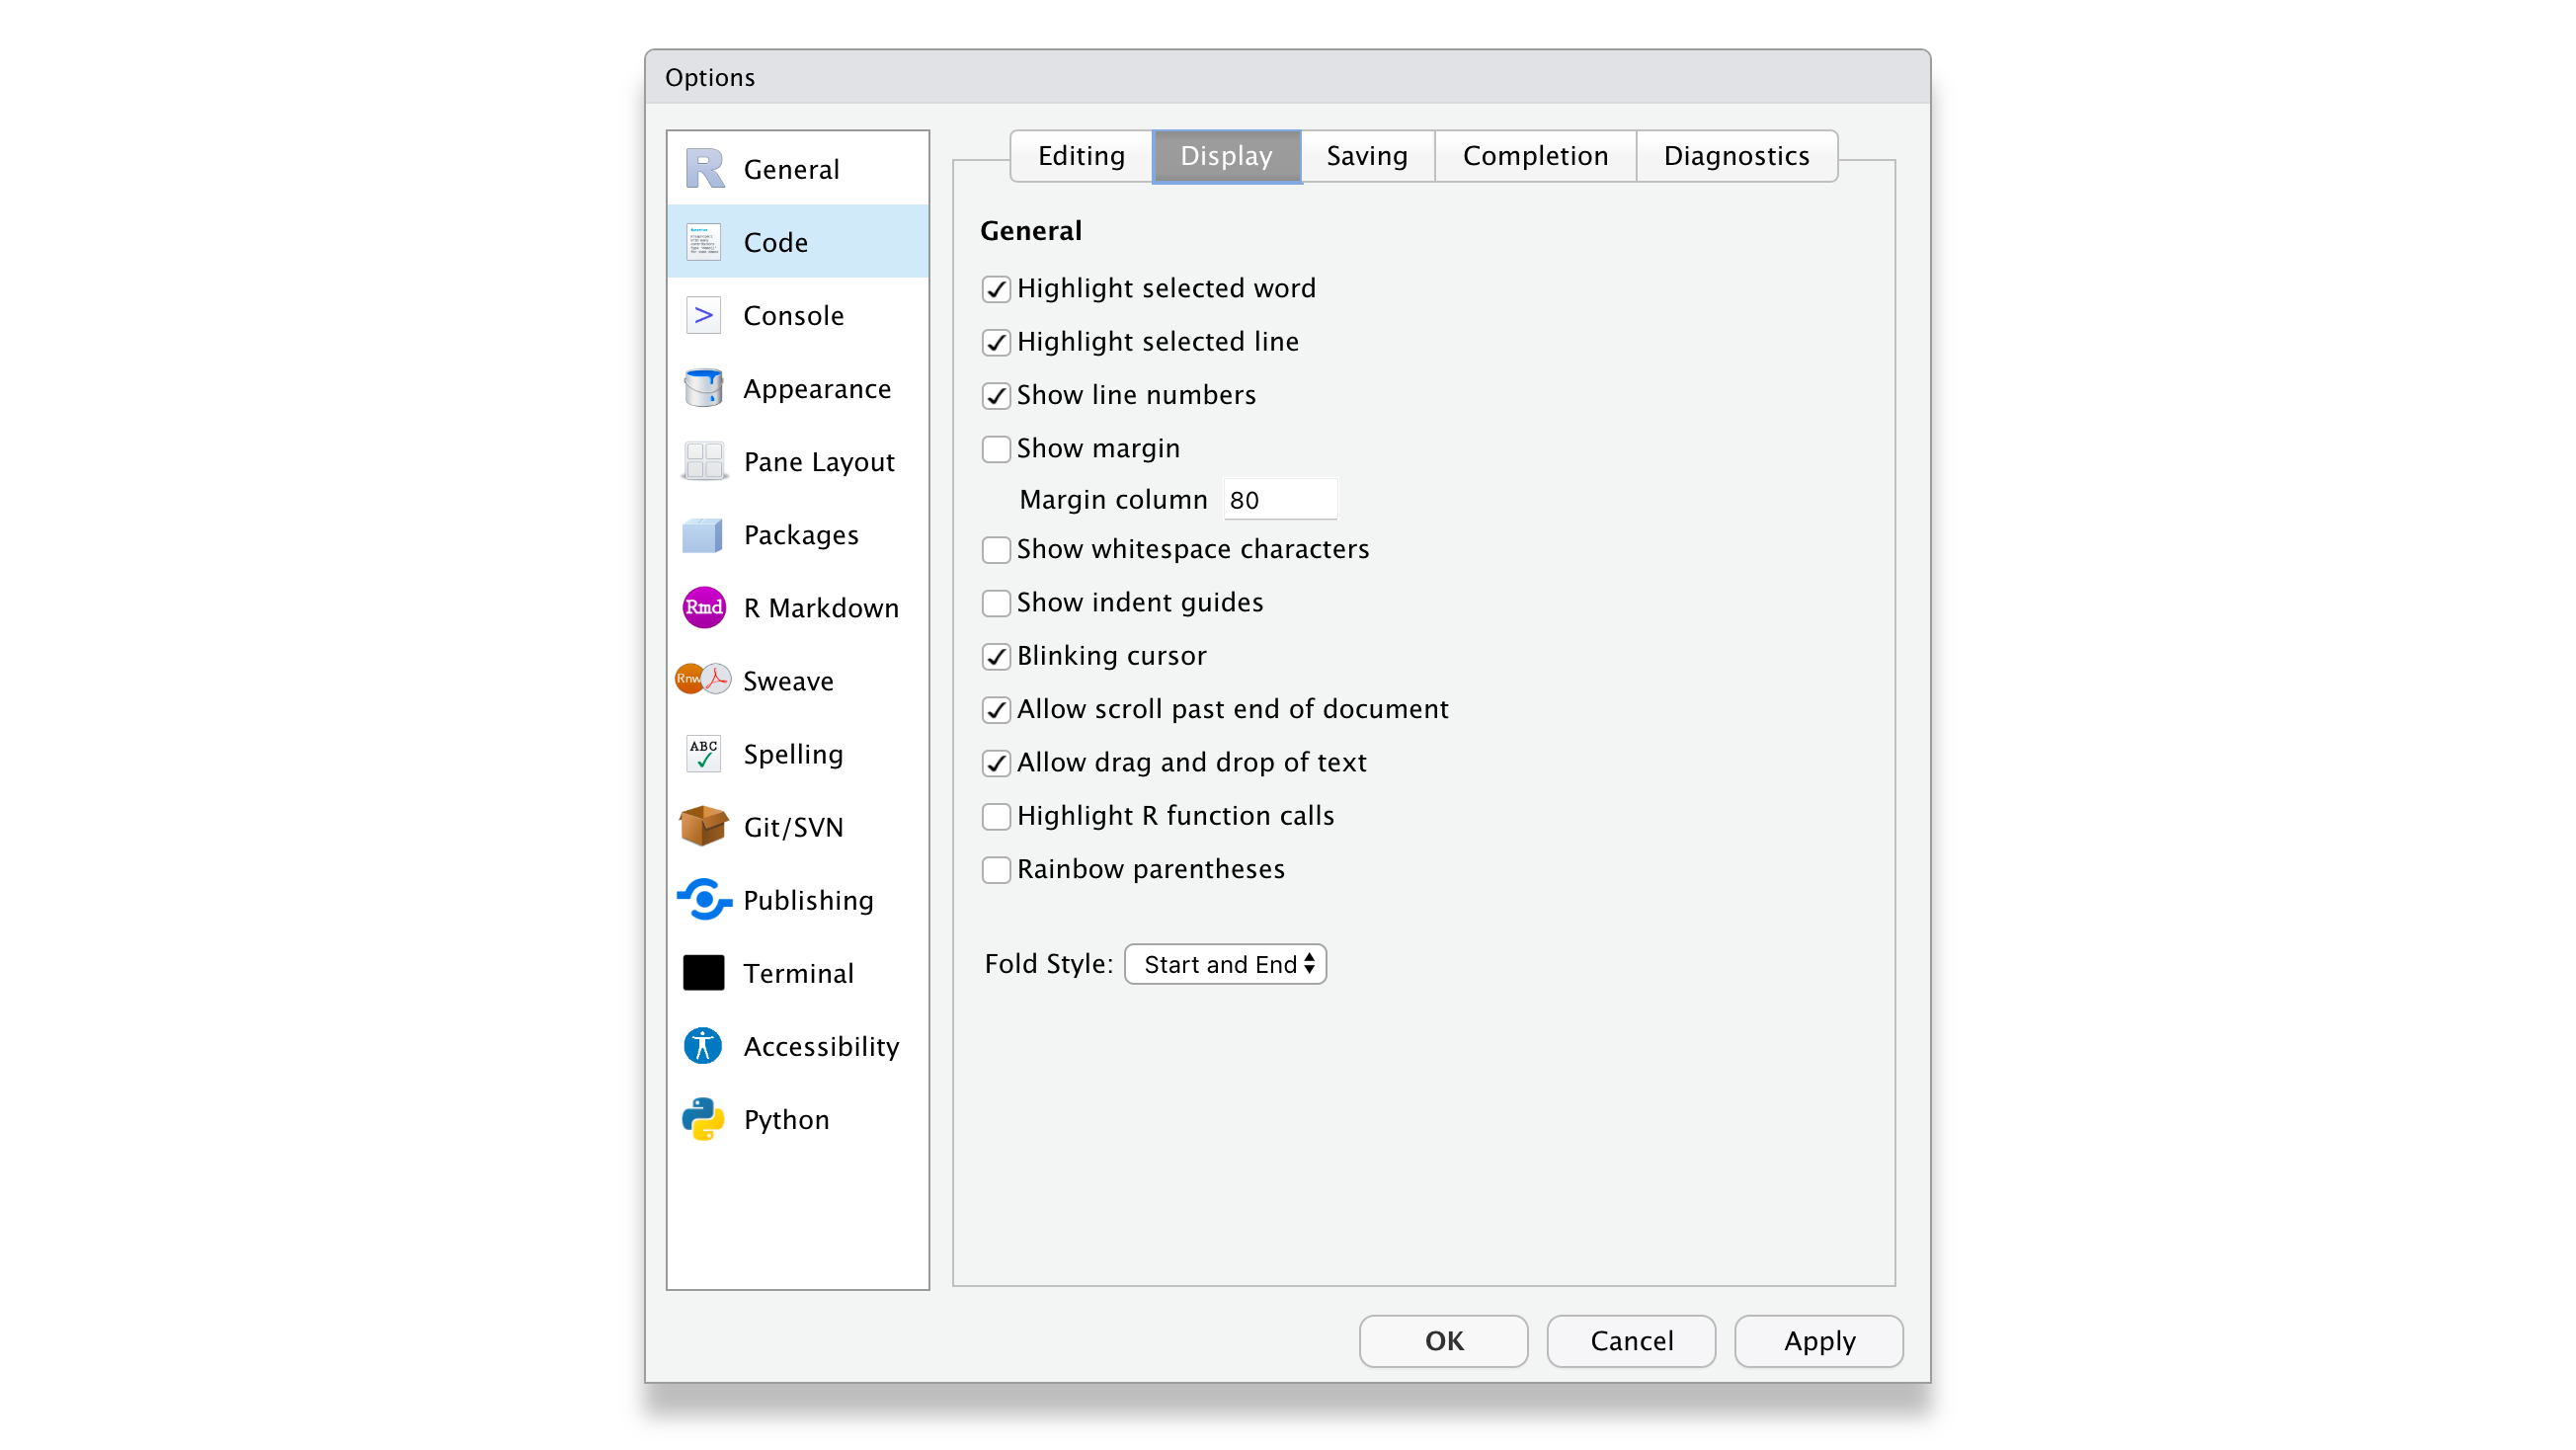
\includegraphics{images/chapter_03_img/rstudio_preferences/02_rstudio_preferences_display.png}
\end{enumerate}

Of course, if you wish to customise your workspace further, you can do
so. The visually most impactful way to alter the default appearance of
RStudio is to select \texttt{Appearance} and pick a completely different
colour theme. Feel free to browse through various options and see what
you prefer. There is no right or wrong here. Just make it your own.

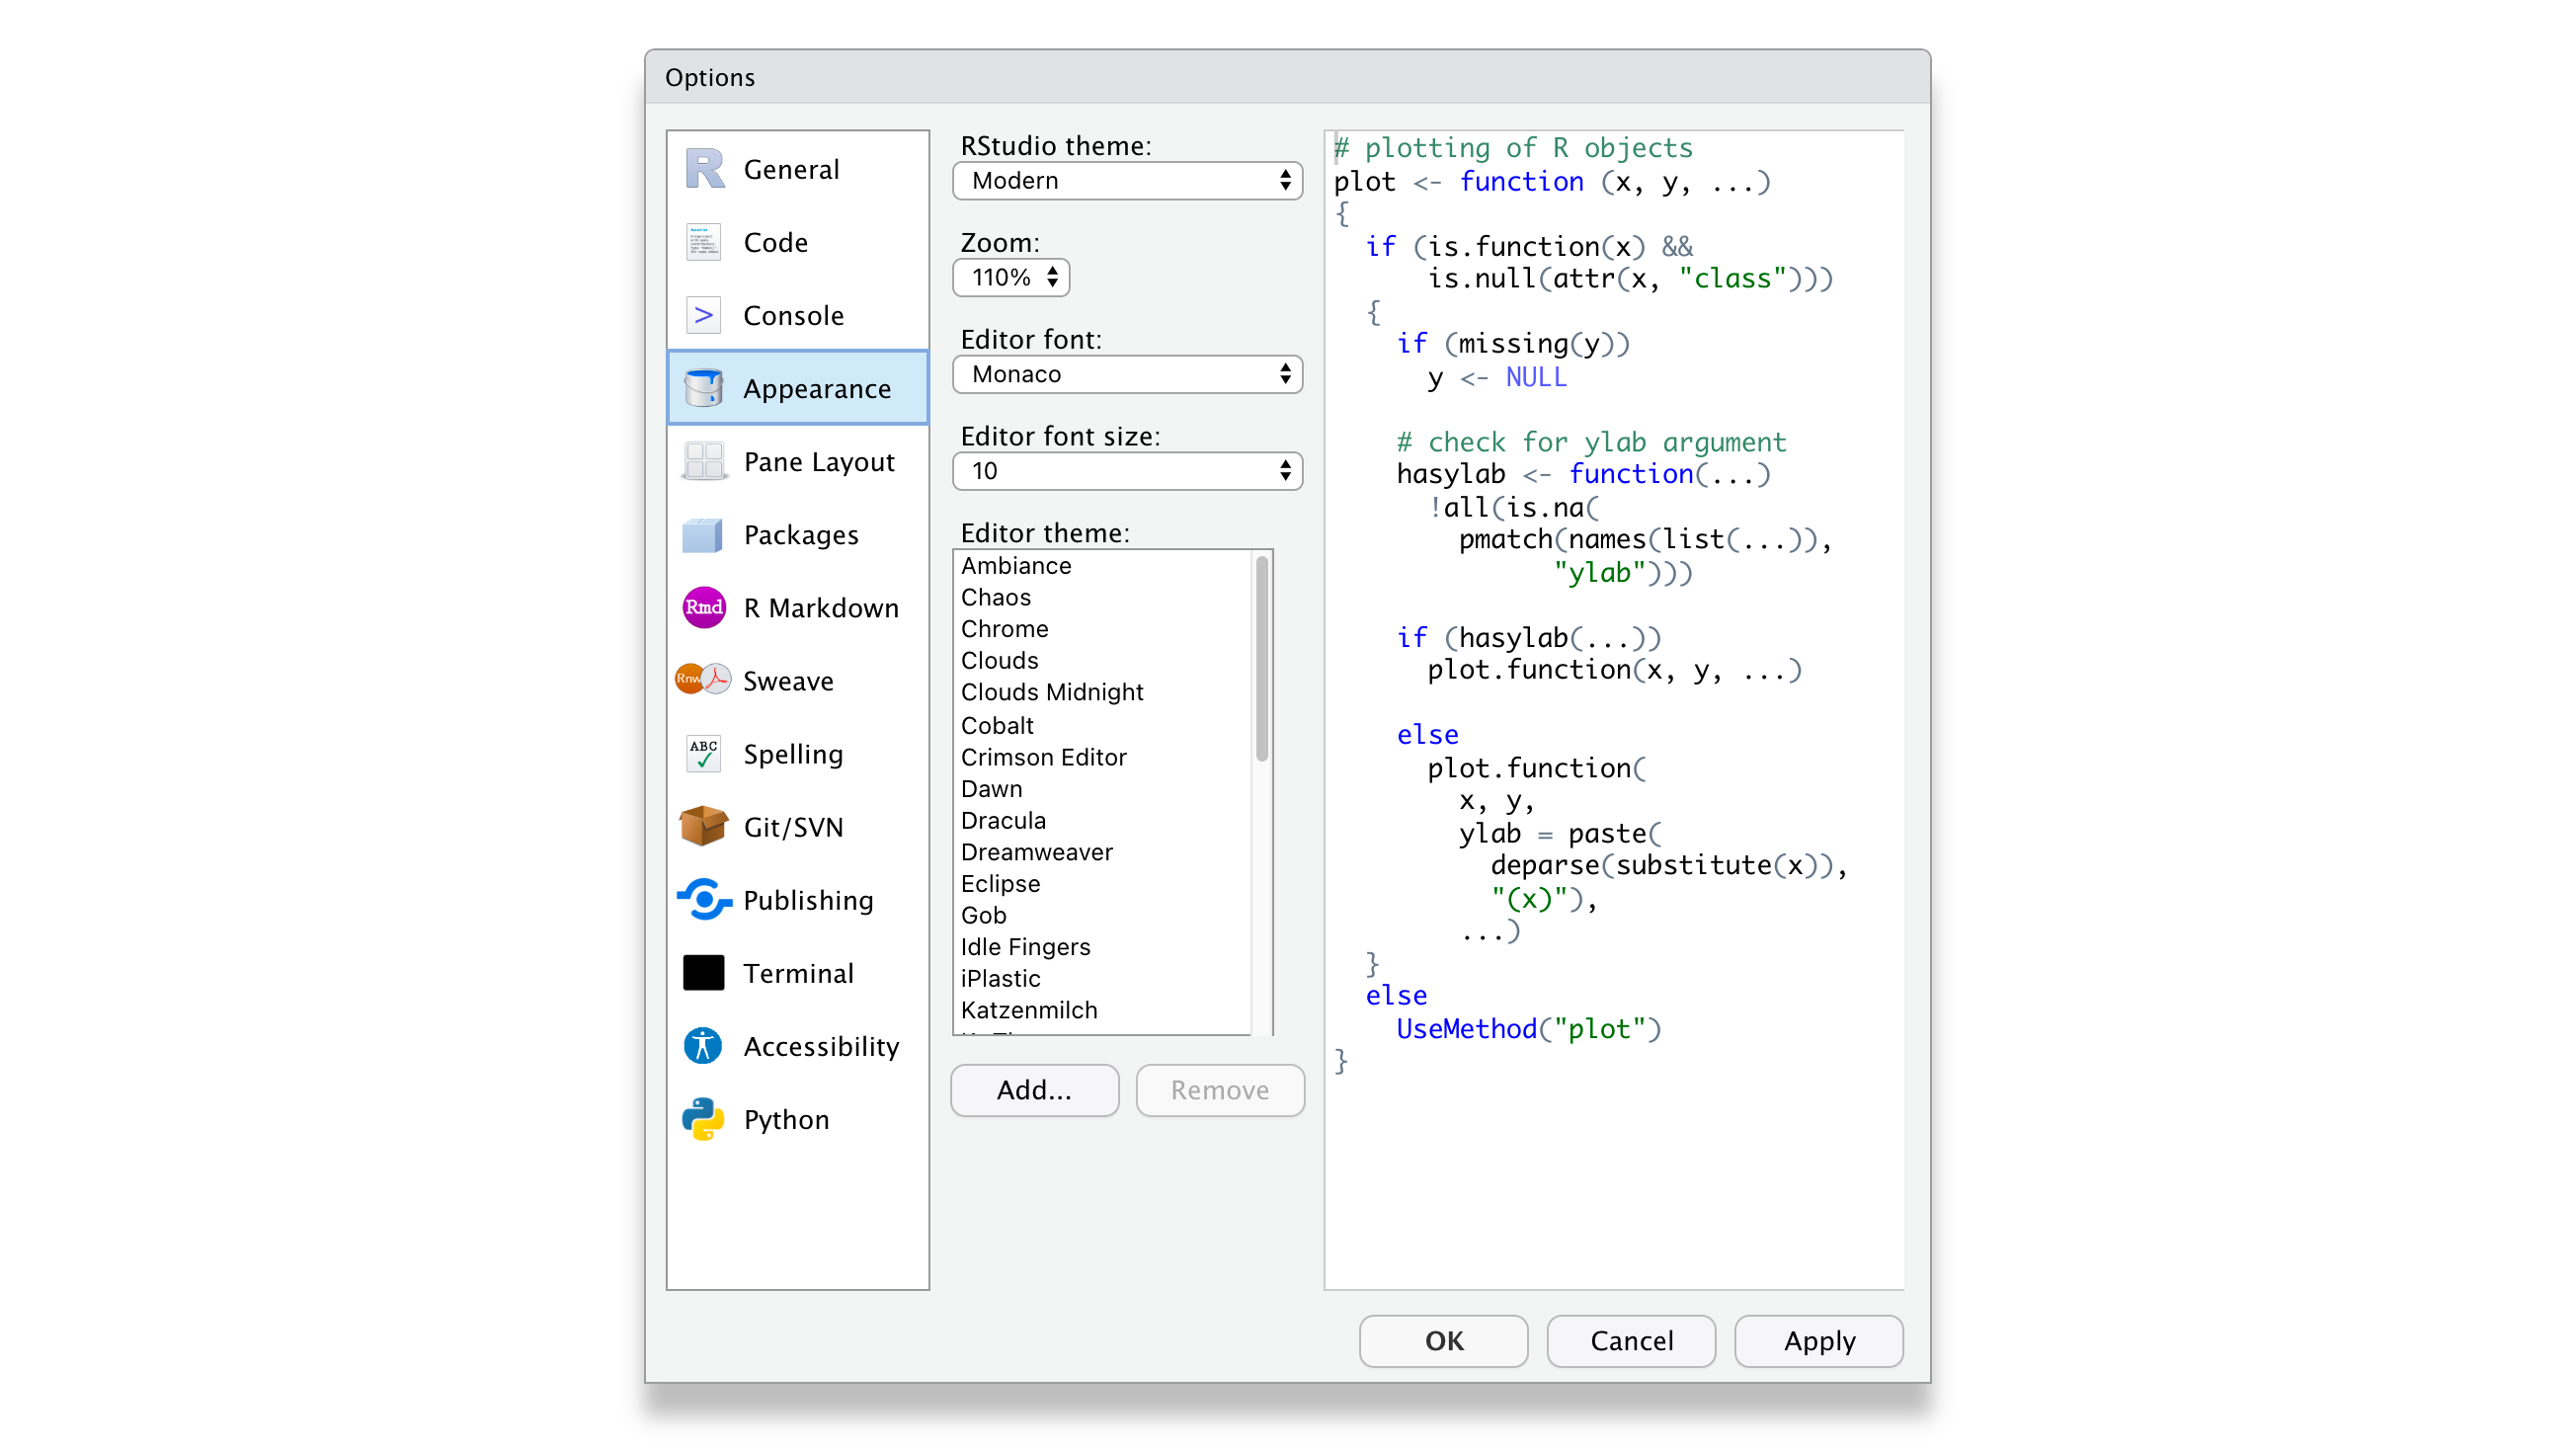
\includegraphics{images/chapter_03_img/rstudio_preferences/03_rstudio_preferences_appearance.png}

\section{Updating R and RStudio: Living at the pulse of
innovation}\label{updating-r-and-rstudio}

While not strictly something that helps you become a better programmer,
this advice might come in handy to avoid turning into a frustrated
programmer. When you update your software, you need to update \emph{R}
and RStudio separately from each other. While both \emph{R} and RStudio
work closely with each other, they still constitute separate pieces of
software. Thus, it is essential to keep in mind that updating RStudio
will not automatically update R. This can become problematic if specific
tools you installed via RStudio (like a fancy learning algorithm) might
not be compatible with earlier versions of \emph{R}. Also, additional
\emph{R} packages (see Chapter @ref(r-packages)) developed by other
developers are separate pieces which require updating too, independently
from \emph{R} and RStudio.

I know what you are thinking: This already sounds complicated and
cumbersome. However, rest assured, we take a look at how you can easily
update all your packages with RStudio. Thus, all you need to remember
is: \emph{R} needs to be updated separately from everything else.

\section{RStudio Cloud}\label{rstudio-cloud}

RStudio Cloud is an application that runs in your web browser. It allows
you to write and access \emph{R} code wherever you go. It even works on
your tablet because it does not require installation. However, do expect
it to run slower if your internet connection is not fast or stable. To
work with RStudio Cloud, you also need an internet connection. However,
there are many benefits to using RStudio in the cloud, such as running
time-consuming scripts without using your own device. Also, it is much
easier to collaborate with others, and since no installation is
required, you can work on projects on any device as long as you are
connected to the internet. However, RStudio Cloud's most significant
advantage is that you can get started with programming within seconds
compared to a desktop installation. Still, I prefer my locally-run
offline version of RStudio, because I appreciate working offline as much
as online. Nevertheless, I recommend setting up an account because you
never know when you need it.

To get started with RStudio Cloud, we have to undertake a couple of
steps:

\begin{enumerate}
\def\labelenumi{\arabic{enumi}.}
\item
  Open your web browser of choice and navigate to
  \url{https://rstudio.cloud}.

  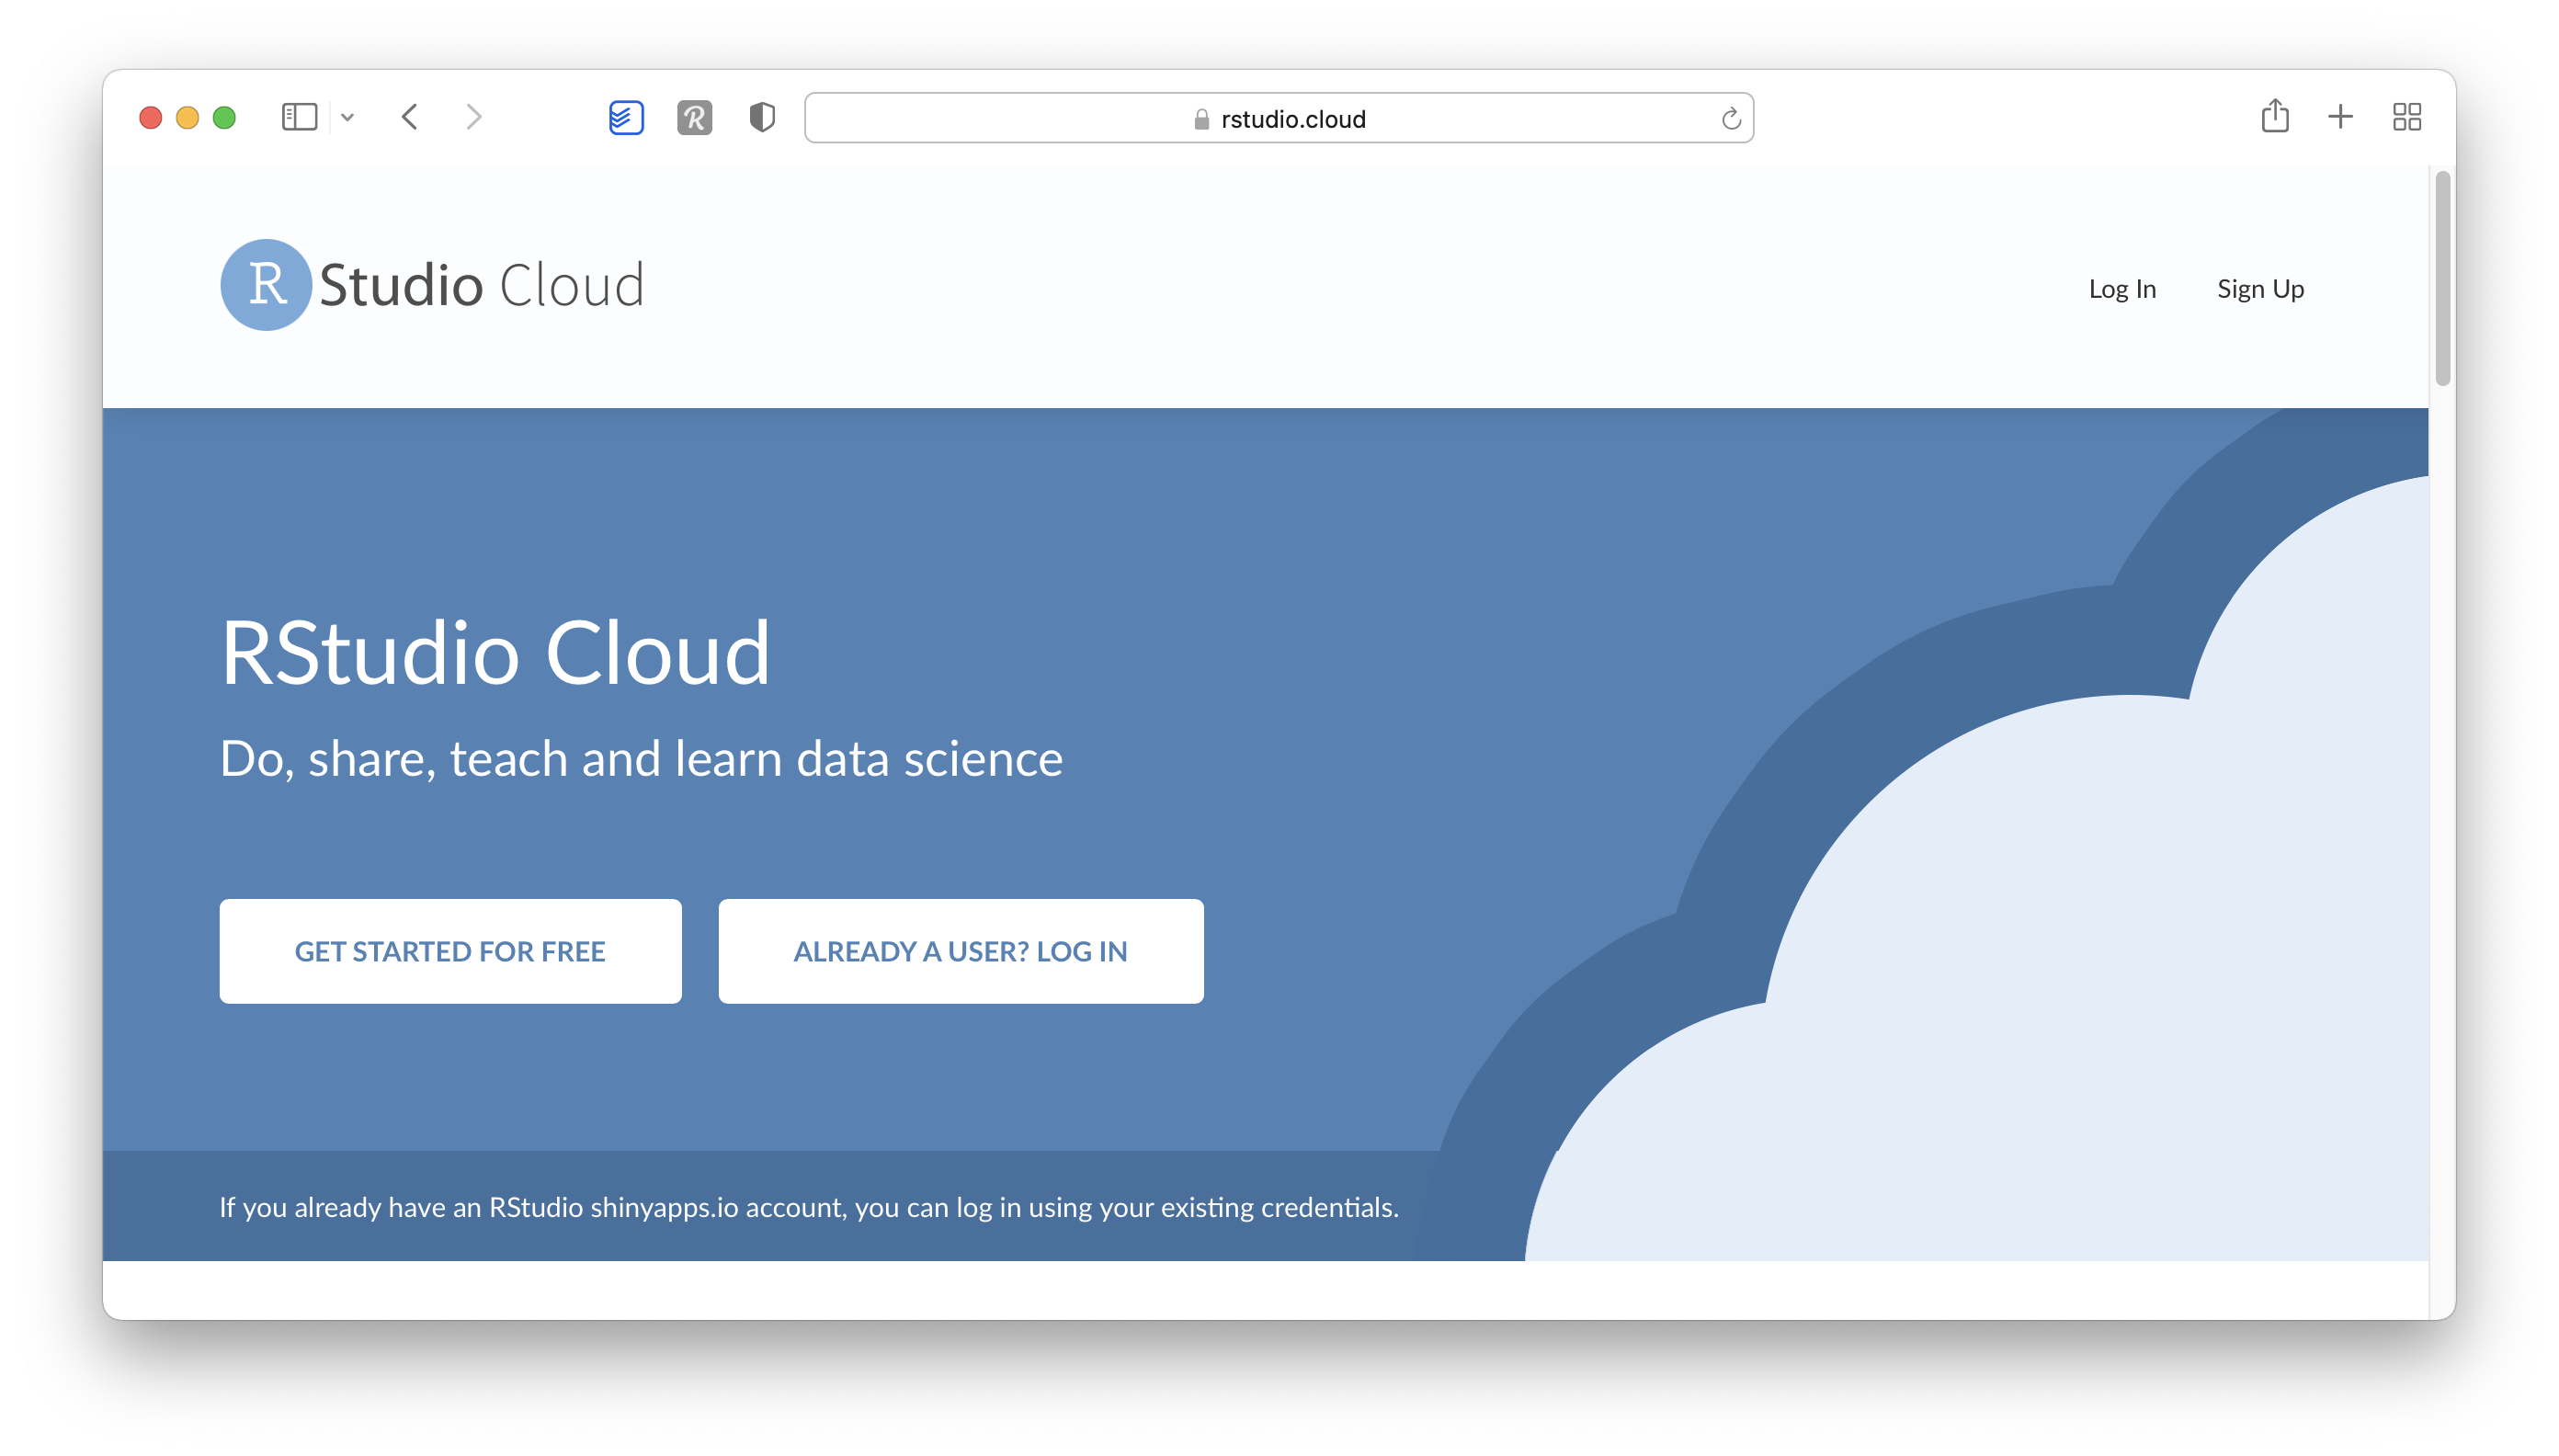
\includegraphics{images/chapter_03_img/rstudio_cloud/01_rstudio_cloud.png}
\item
  Click on \texttt{Sign\ Up} to create your account.
\item
  On the next page, make sure you have the free plan selected and click
  on \texttt{Sign\ up}.

  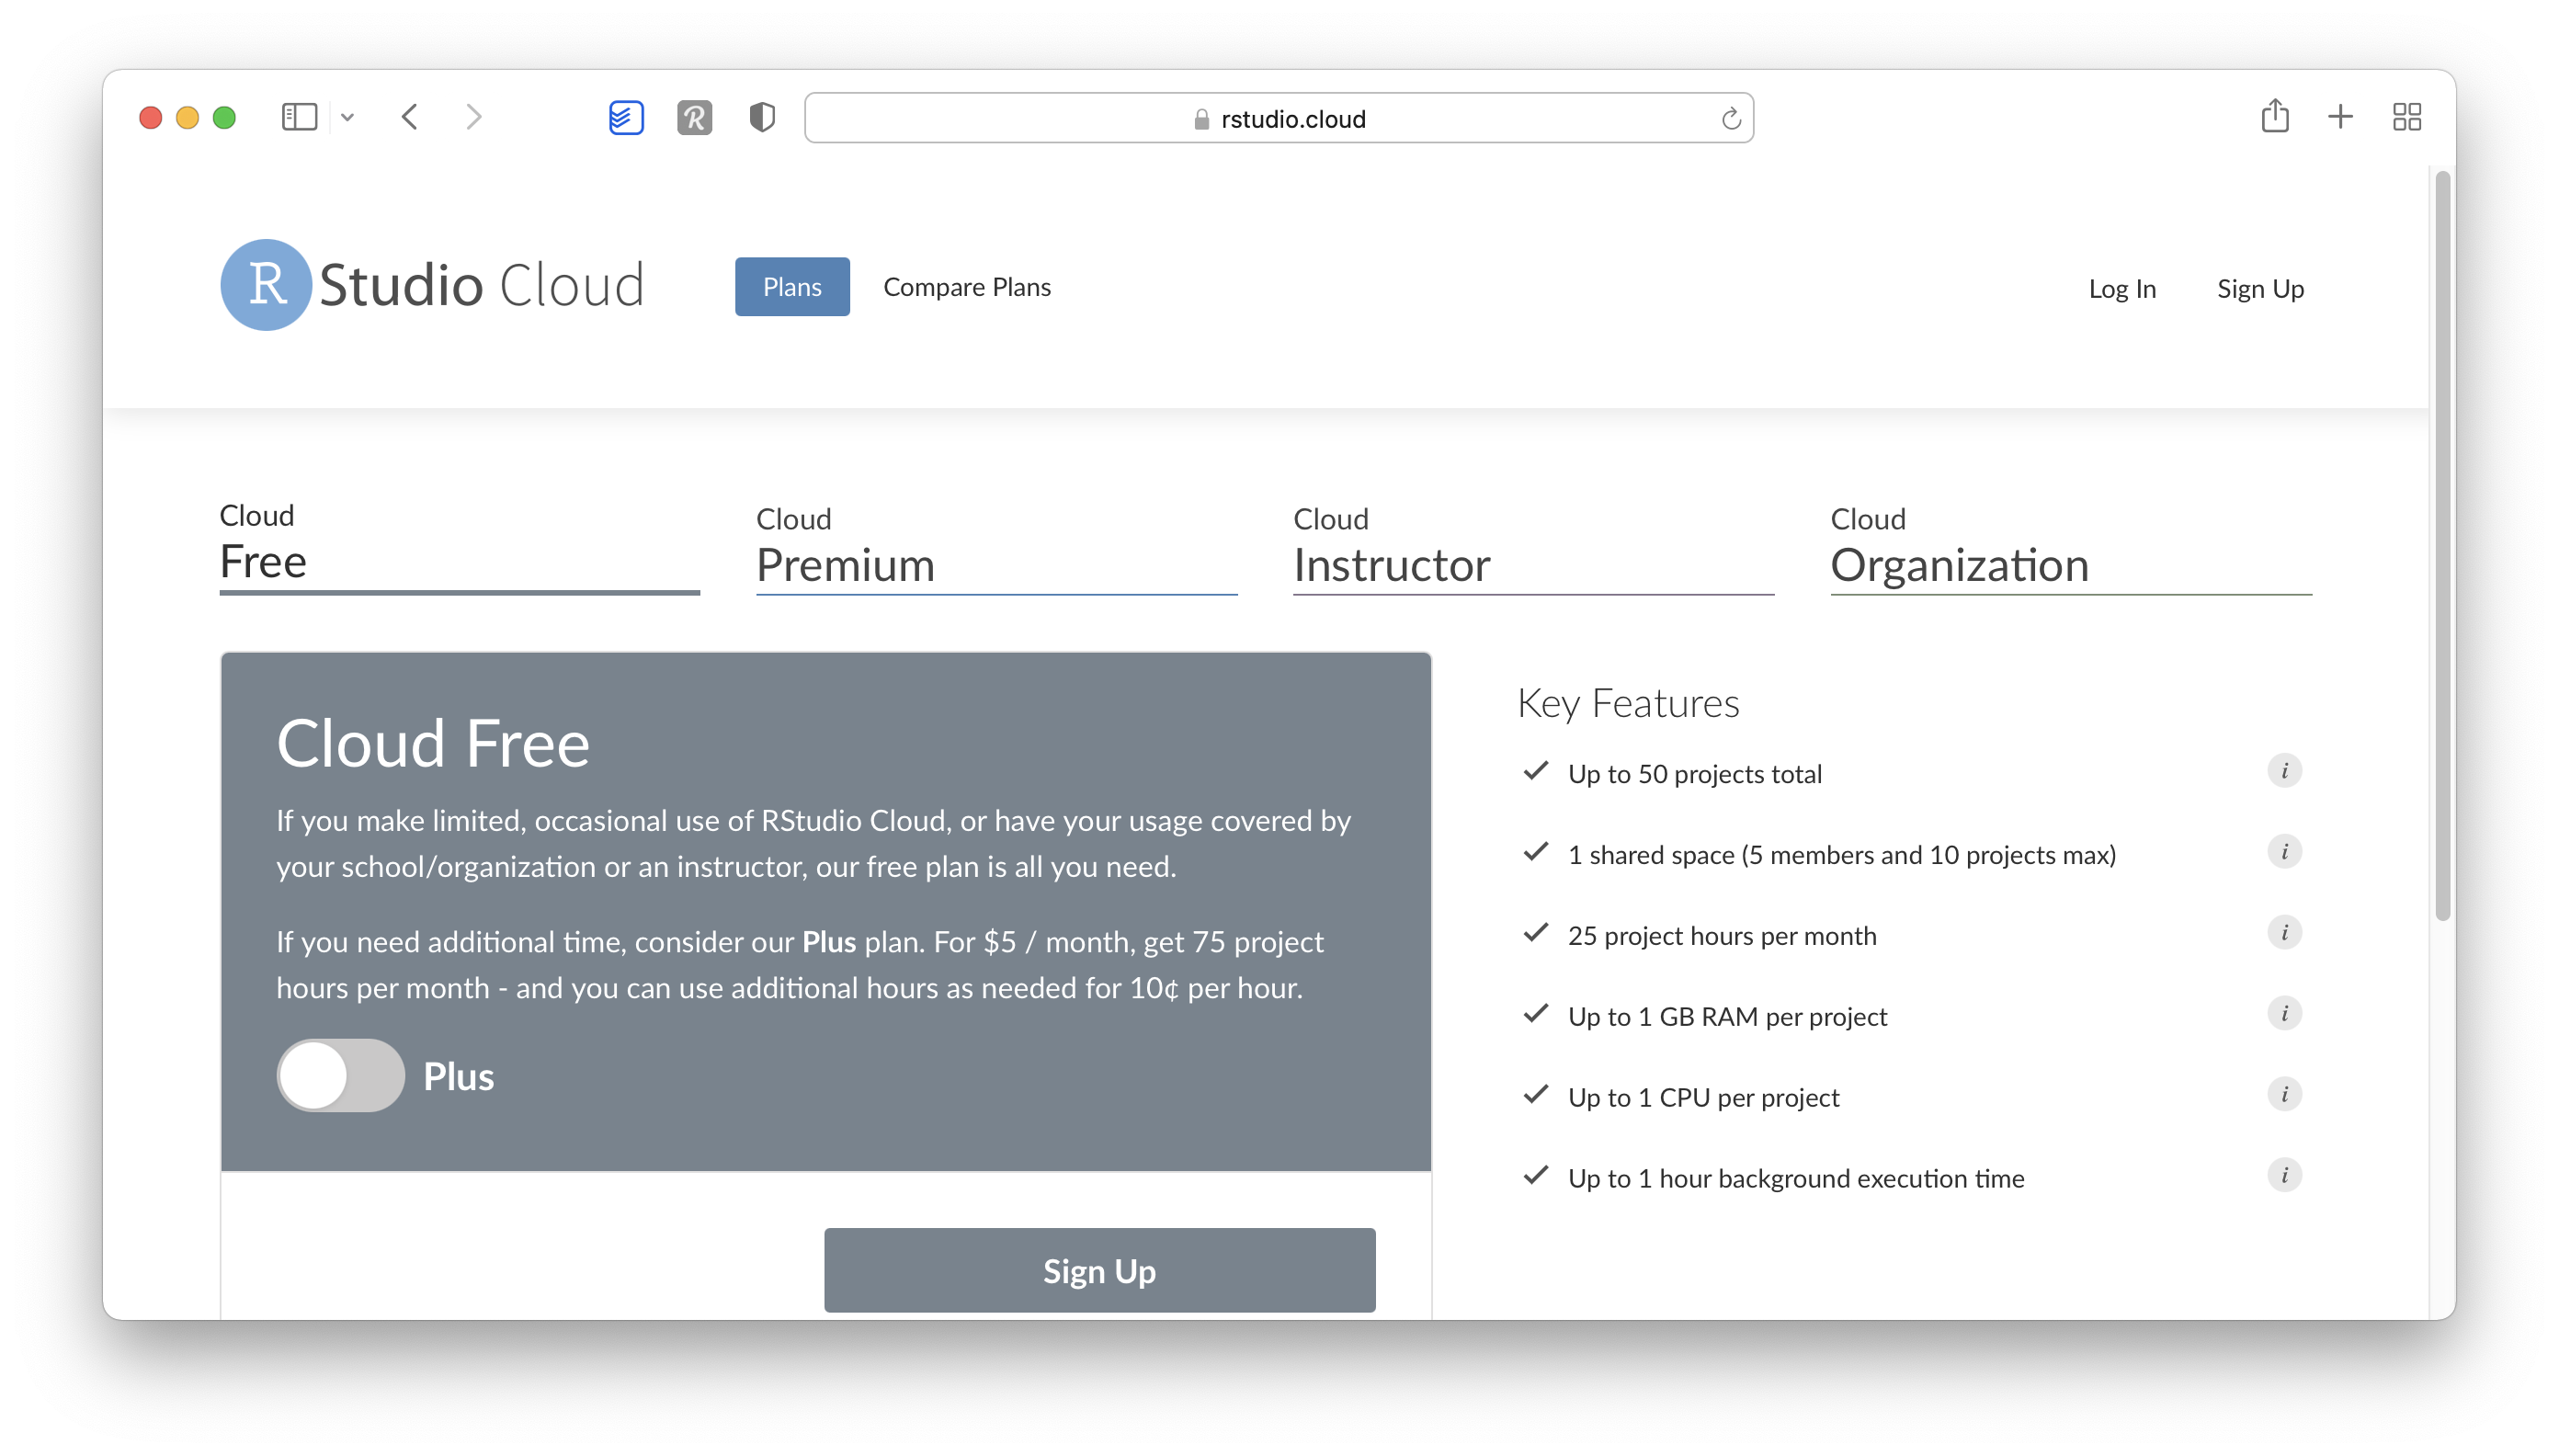
\includegraphics{images/chapter_03_img/rstudio_cloud/02_rstudio_cloud.png}
\item
  To finalise the registration process, you are required to provide your
  credentials.

  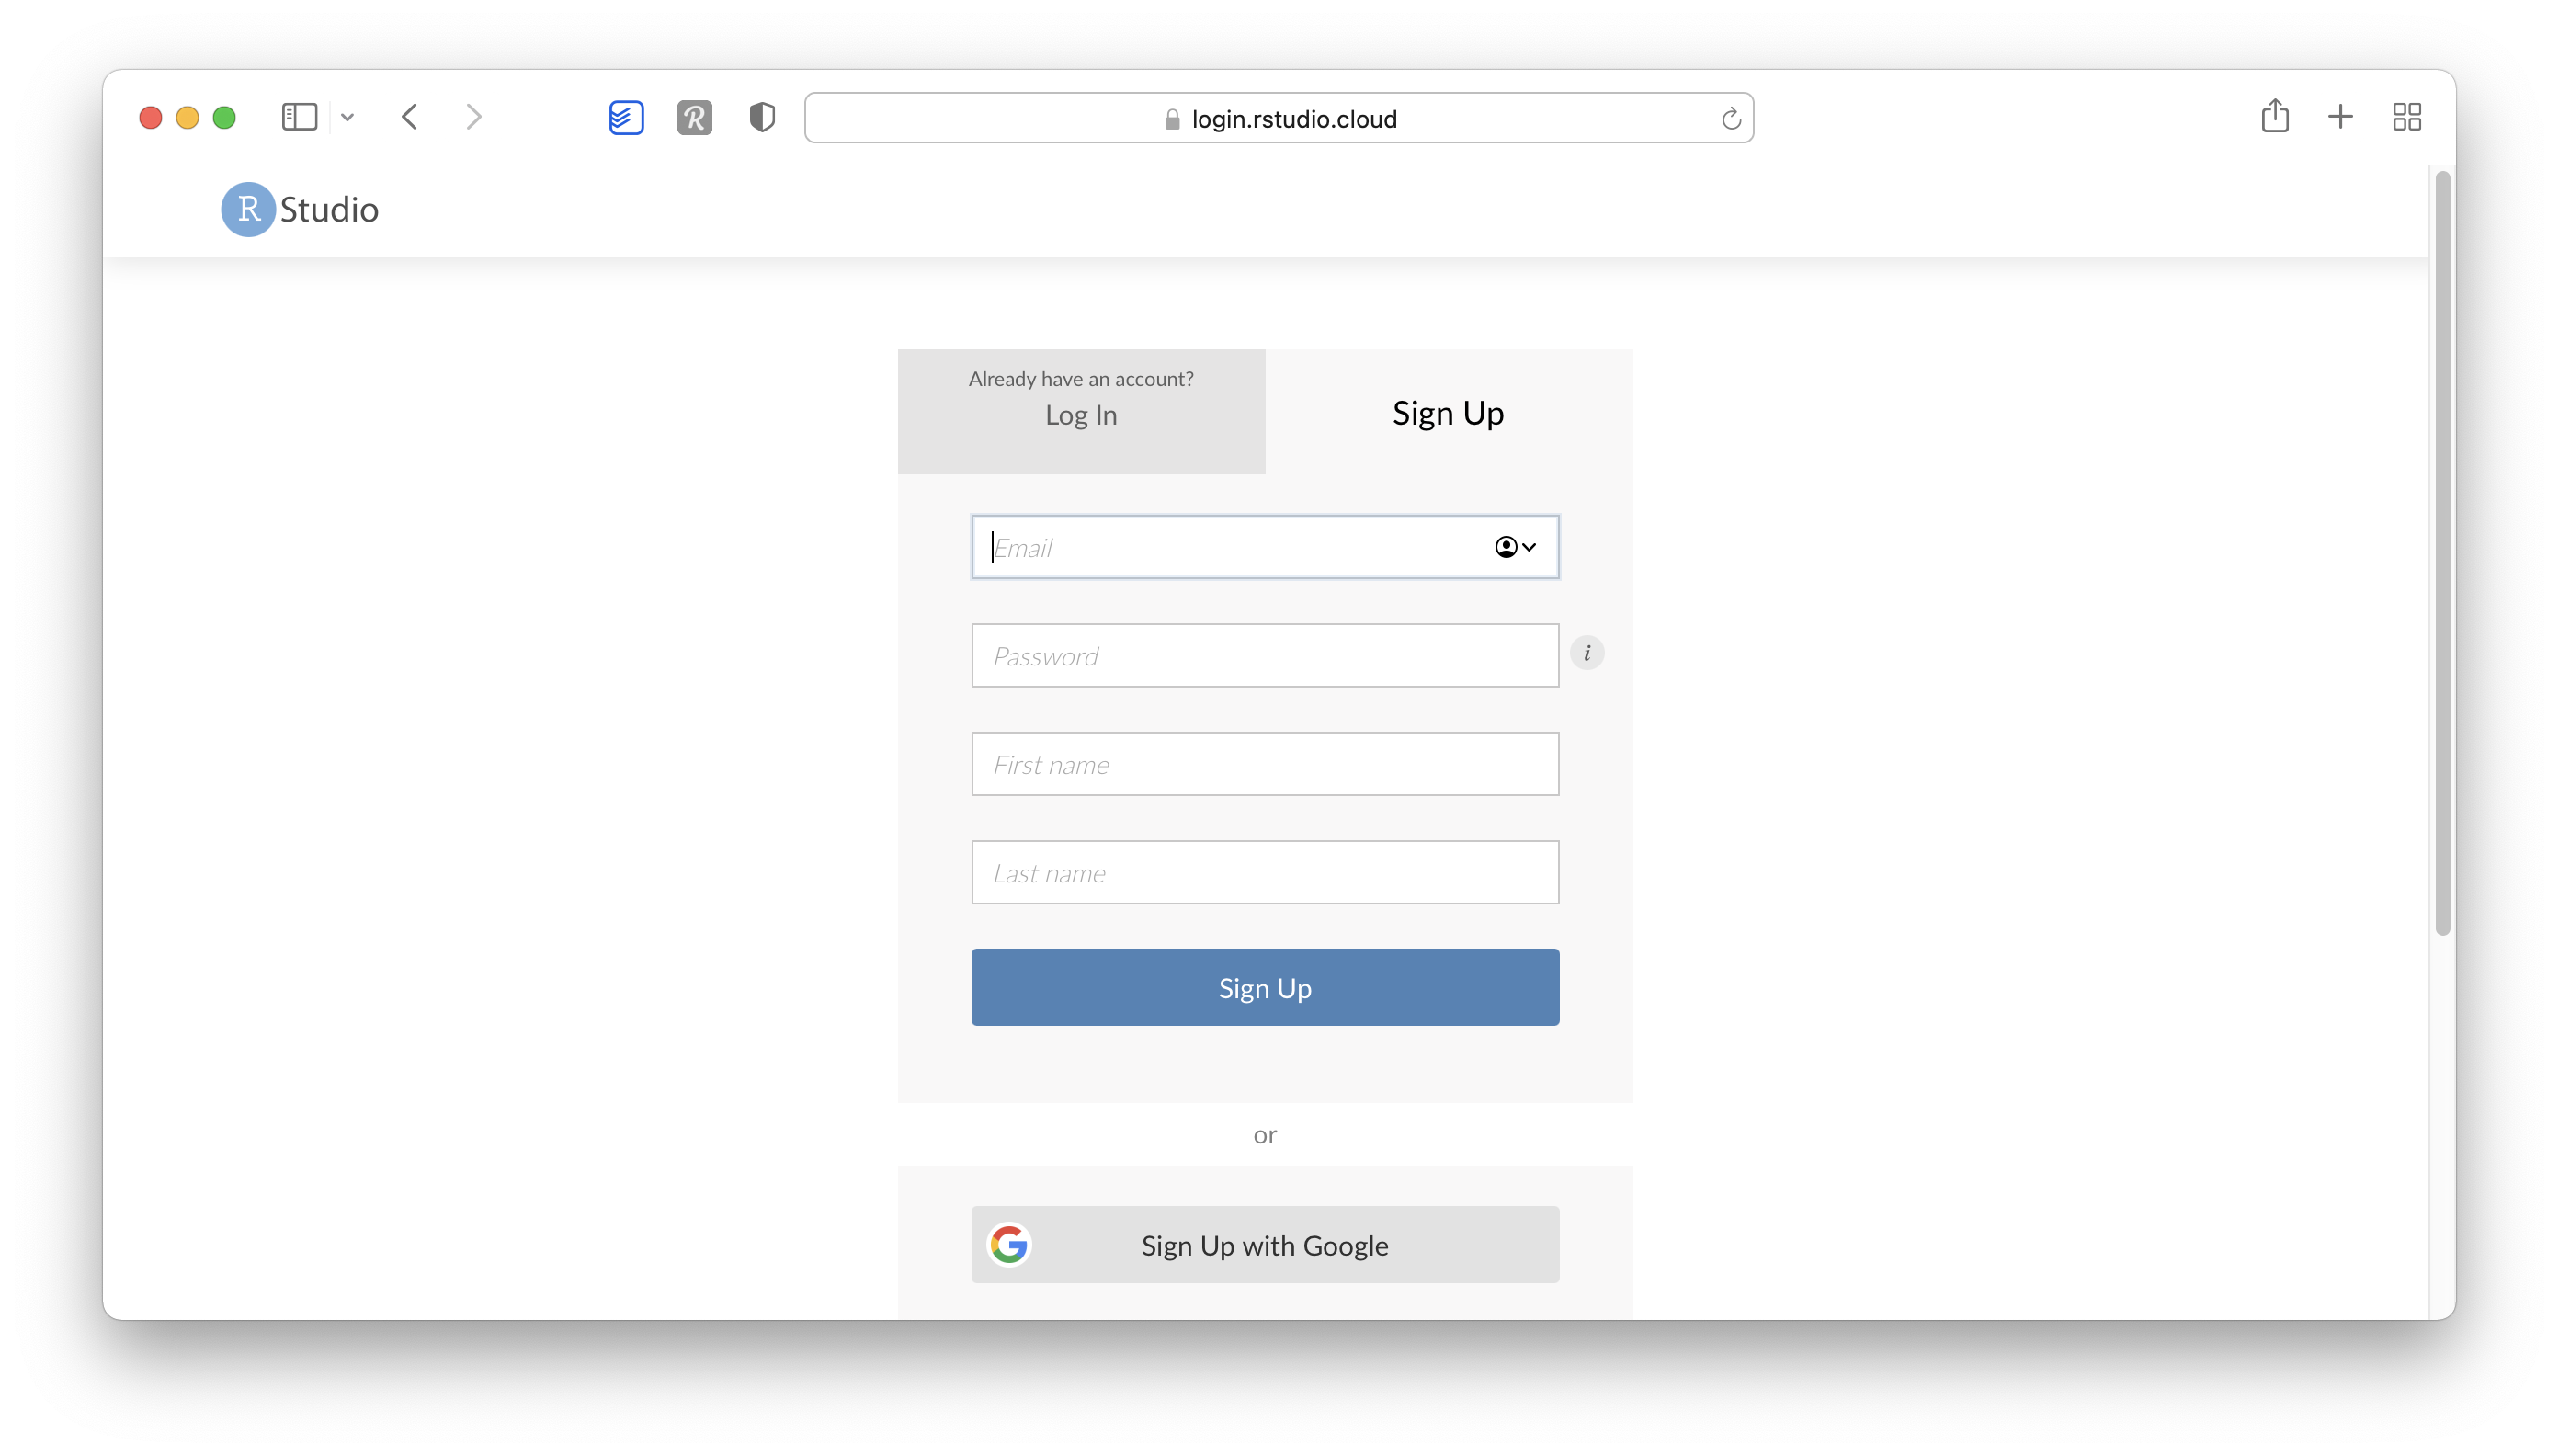
\includegraphics{images/chapter_03_img/rstudio_cloud/03_rstudio_cloud.png}
\item
  Once you complete your registration, you are redirected to
  \texttt{Your\ Workspace}, the central hub for all your projects. As
  you can tell, I already added another workspace called
  \texttt{R\ for\ Non-Programmers}. However, it is fine to use the
  default one.

  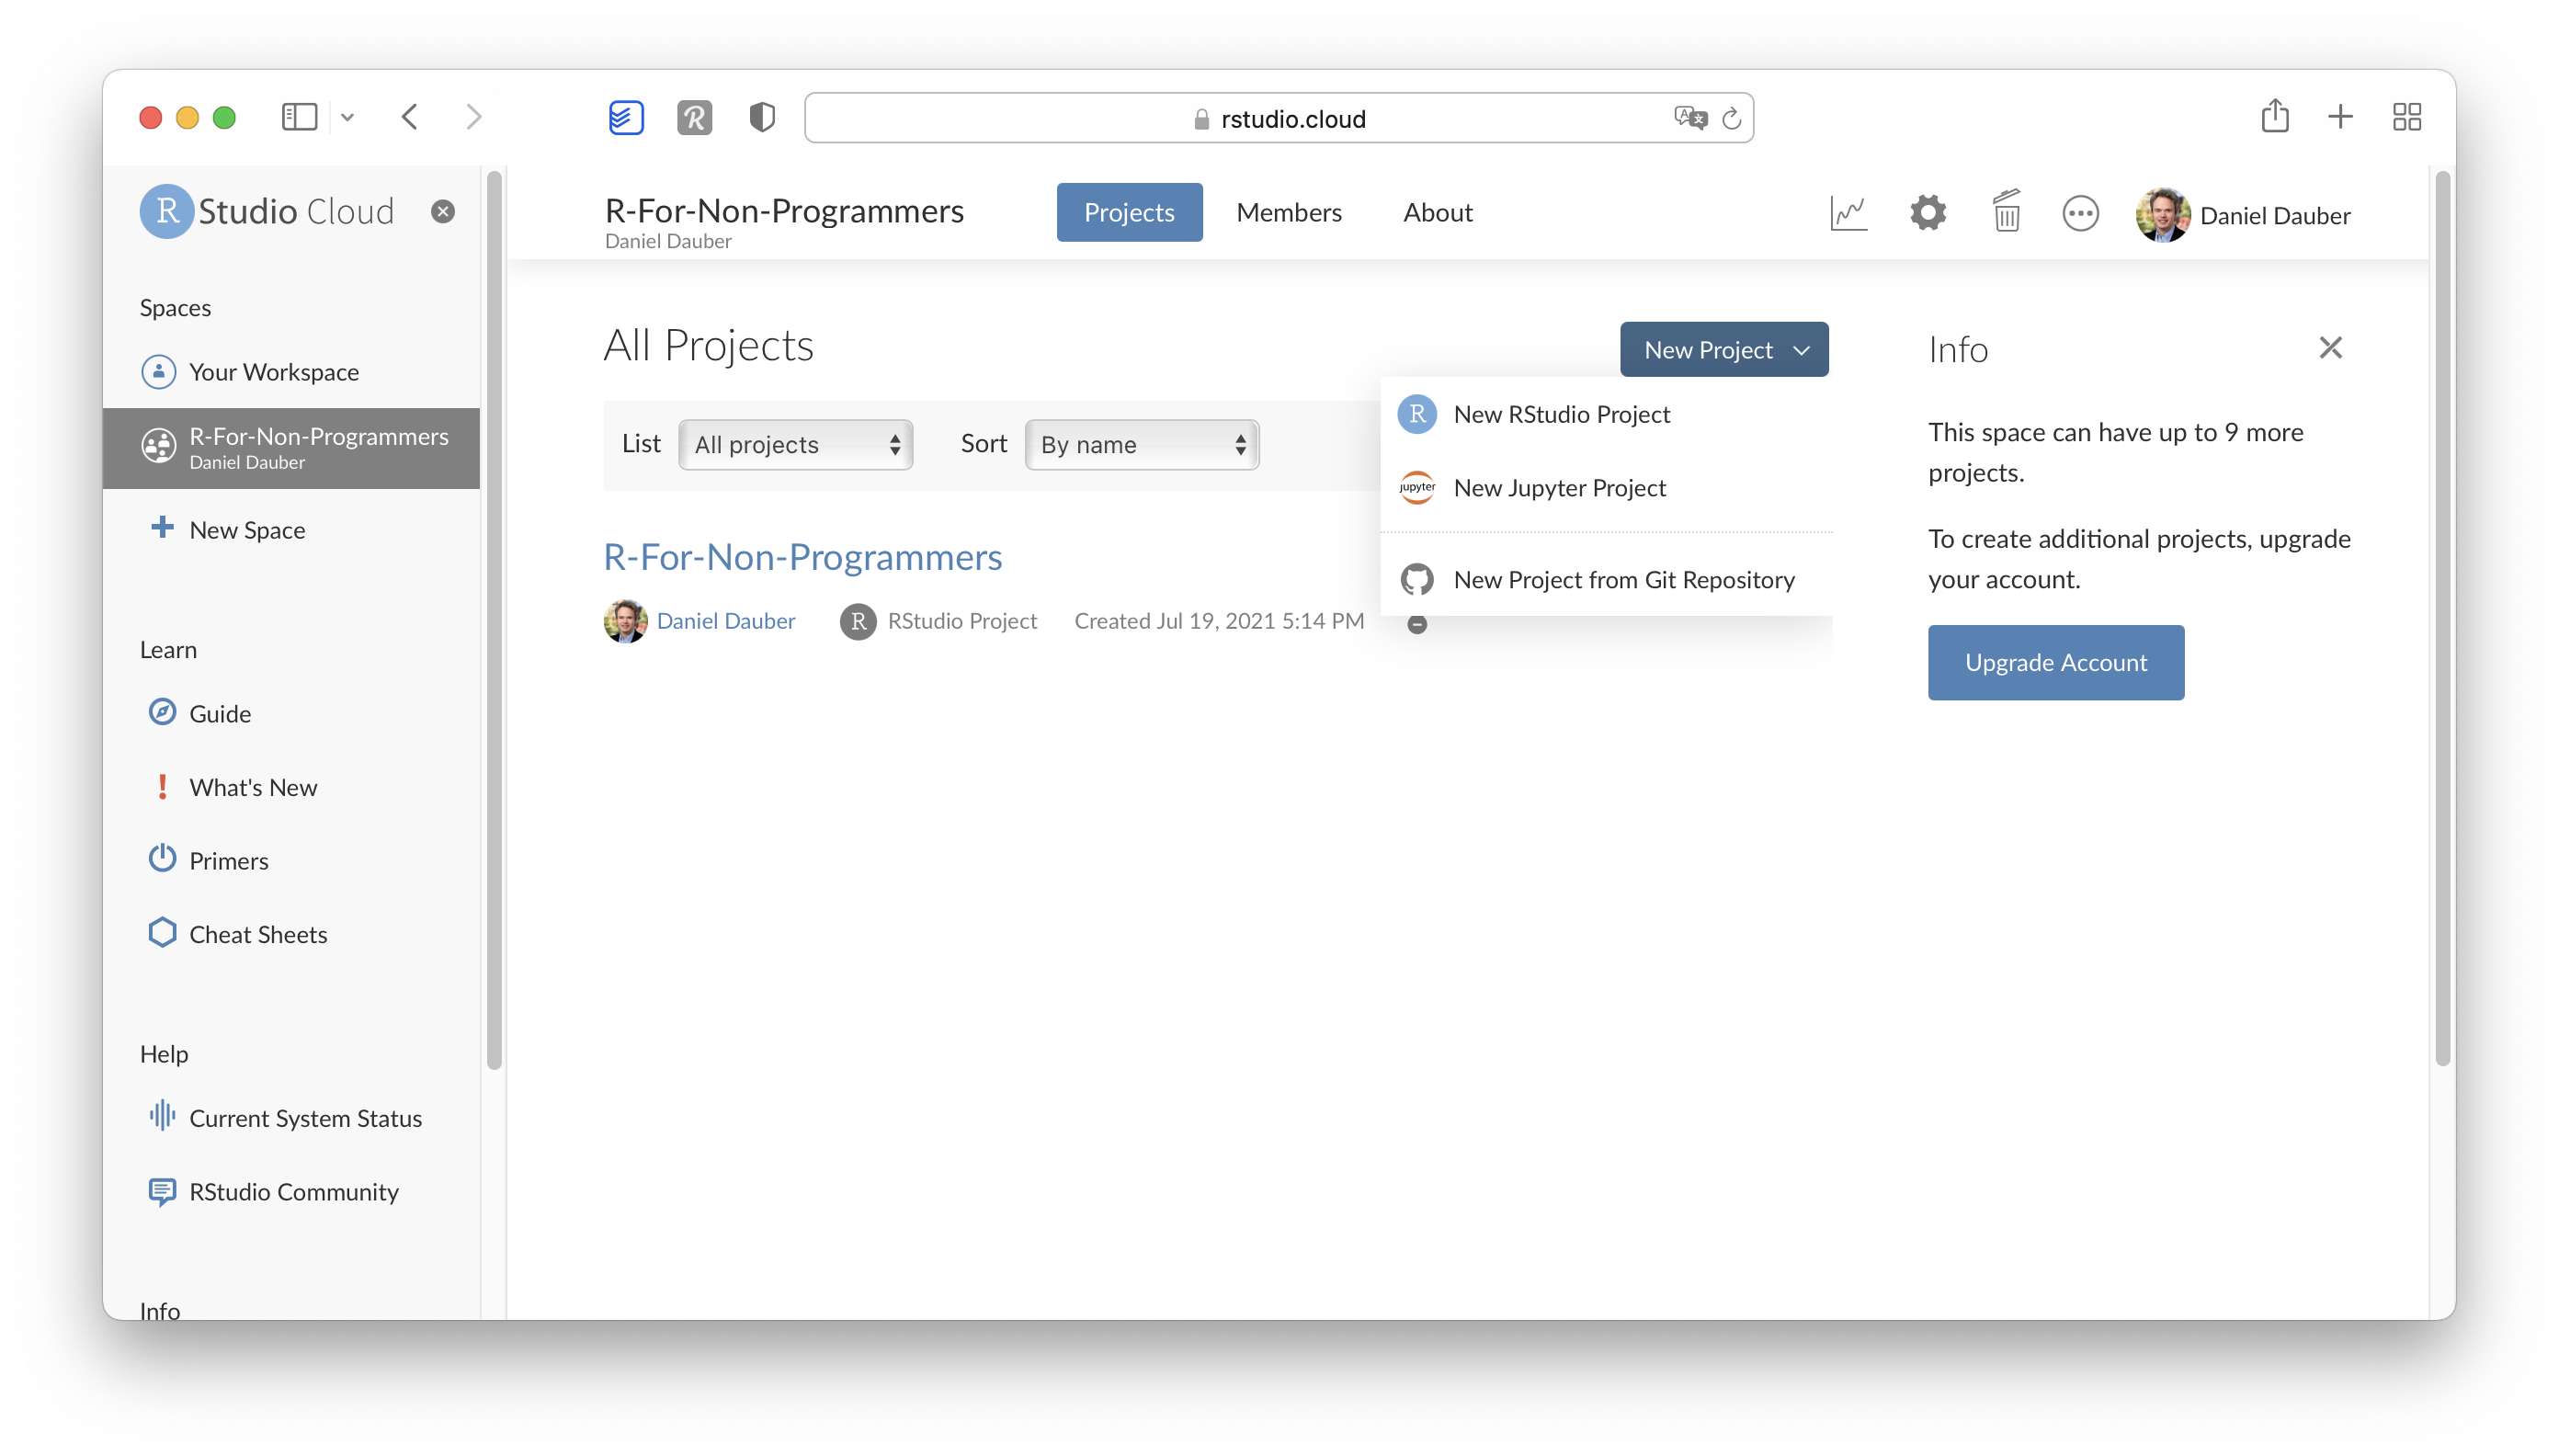
\includegraphics{images/chapter_03_img/rstudio_cloud/05_rstudio_cloud.png}
\item
  To start a new \emph{R} project, you can click on
  \texttt{New\ Project\ \textgreater{}\ New\ RStudio\ Project}. This
  will open RStudio in the Cloud, which looks identical to the desktop
  version. You can immediately start writing your code. The example
  below computes a plot.\footnote{RStudio and RStudio Cloud warn you if
    you need to install certain R packages to successfully run code.
    More about R packages and what they are can be found in Chapter
    @ref(r-packages).}

  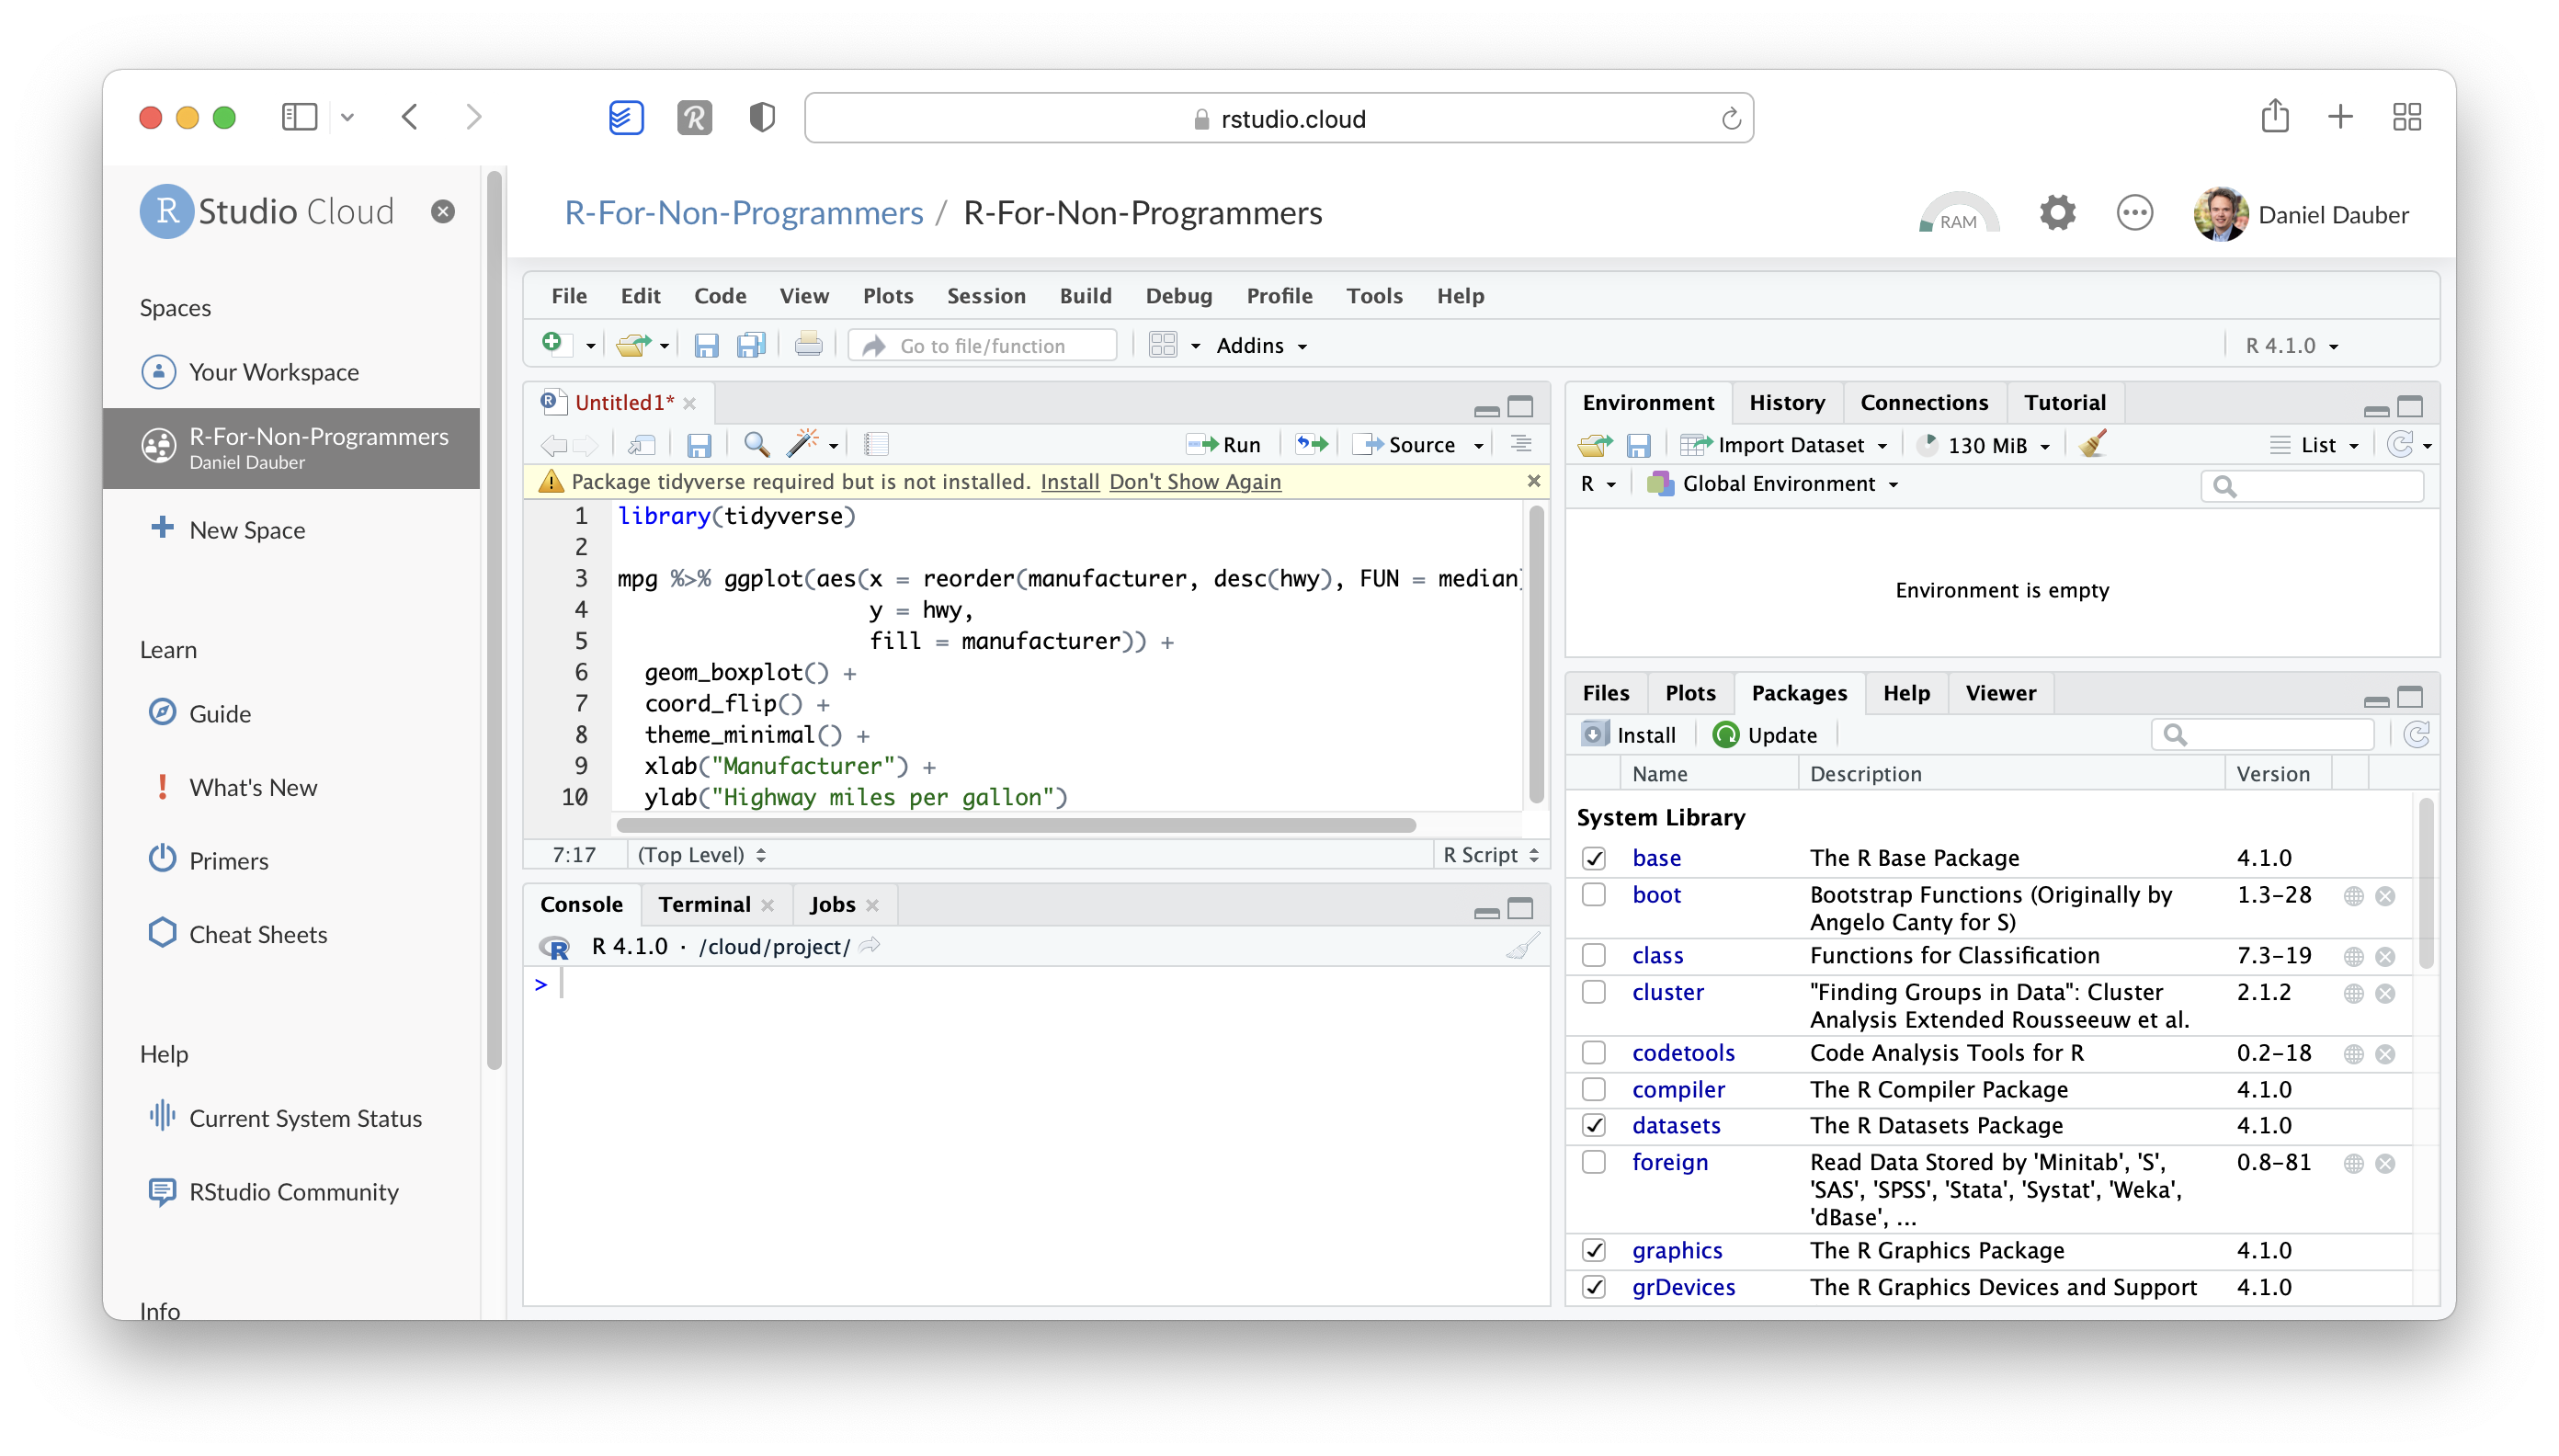
\includegraphics{images/chapter_03_img/rstudio_cloud/06_rstudio_cloud.png}
\item
  Now we can execute the code as we would on the desktop version (see
  Chapter @ref(r-basics-the-very-fundamentals)).

  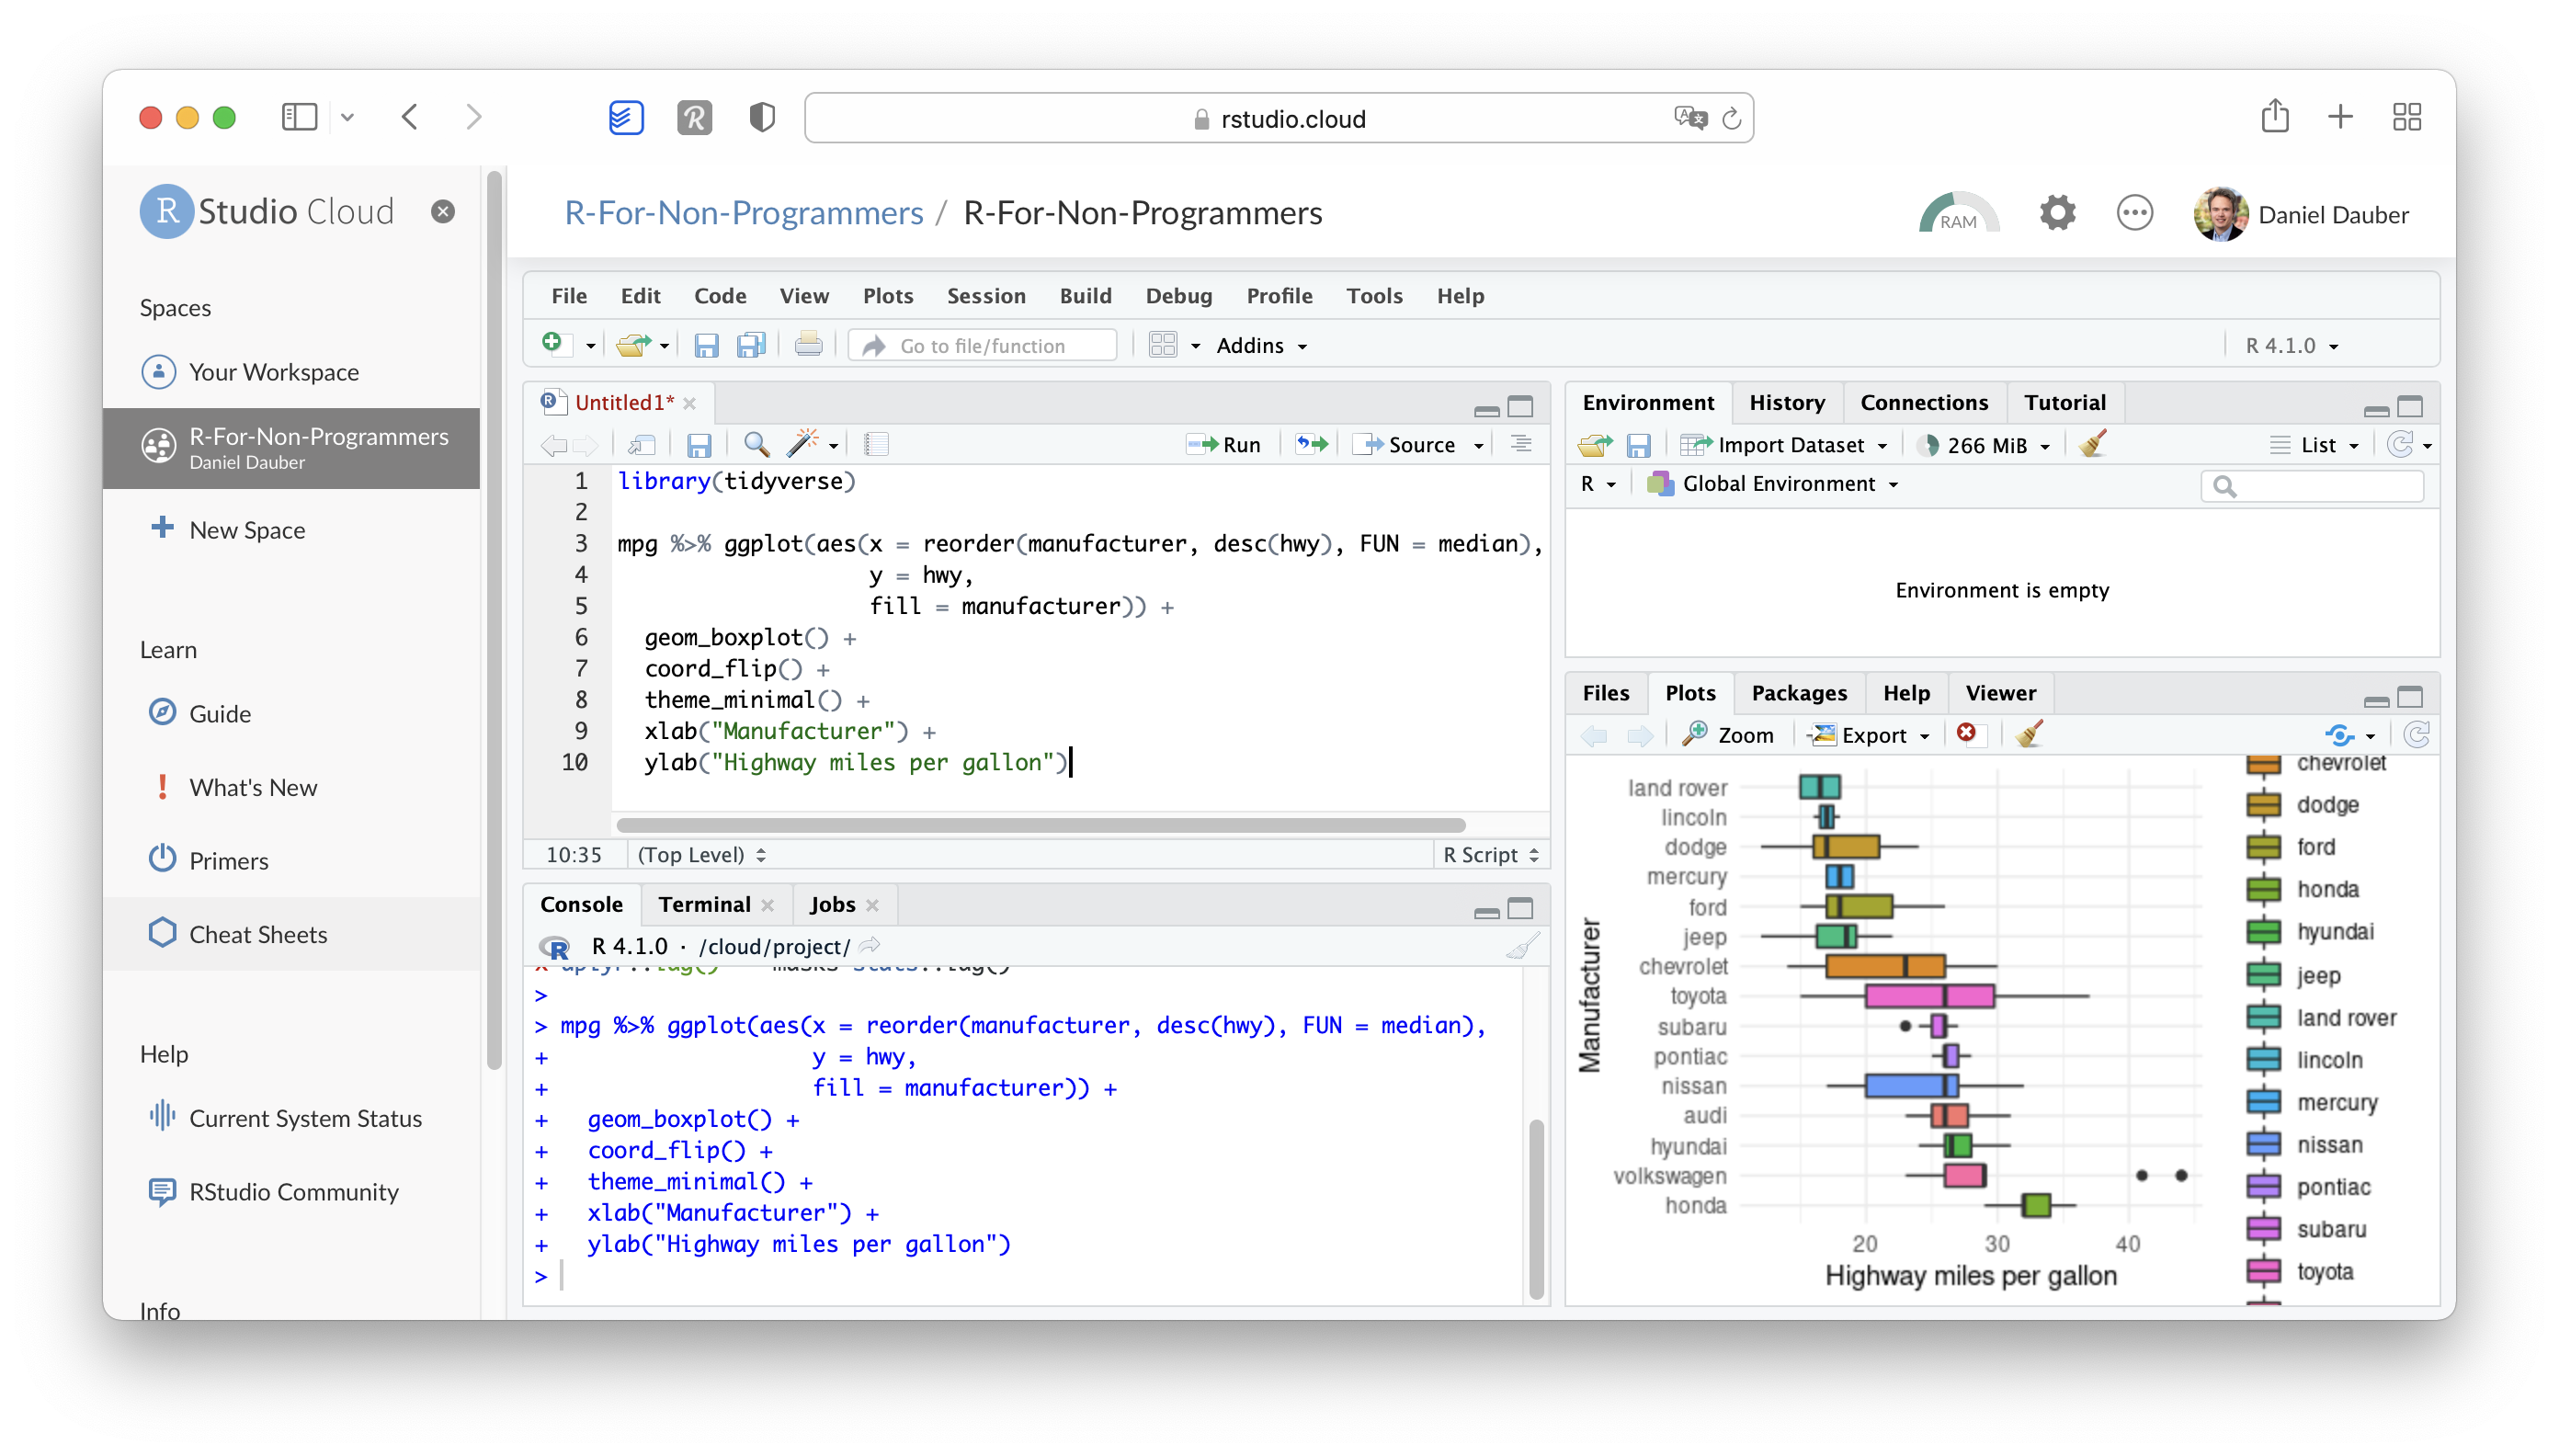
\includegraphics{images/chapter_03_img/rstudio_cloud/07_rstudio_cloud.png}
\end{enumerate}

No matter whether you choose to use a desktop version of RStudio or
RStudio Cloud, you will be able to follow along in this book with no
problem.

\bookmarksetup{startatroot}

\chapter{The RStudio Interface}\label{the-rstudio-interface}

The RStudio interface is composed of quadrants, each of which fulfils a
unique purpose:

\begin{itemize}
\item
  The \texttt{Console} window,
\item
  The \texttt{Source} window,
\item
  The \texttt{Environment\ /\ History\ /\ Connections\ /\ Tutorial}
  window, and
\item
  The \texttt{Files\ /\ Plots\ /\ Packages\ /\ Help\ /\ Viewer} window
\end{itemize}

Sometimes you might only see three windows and wonder where the
\texttt{Source} window has gone in your version of RStudio. In order to
use it you have to either open a file or create a new one. You can
create a new file by selecting
\texttt{File\ \textgreater{}\ New\ File\ \textgreater{}\ R\ Script} in
the menu bar, or use the keyboard shortcut \texttt{Ctrl\ +\ Shift\ +\ N}
on PC and \texttt{Cmd\ +\ Shift\ +\ N} on Mac.

I will briefly explain the purpose of each window/pane and how they are
relevant to your work in \emph{R}.

\section{The Console window}\label{the-console-window}

The console is located in the bottom-left, and it is where you often
will find the output of your coding and computations. It is also
possible to write code directly into the console. Let's try the
following example by calculating the sum of \texttt{10\ +\ 5}. Click
into the console with your mouse, type the calculation into your console
and hit \texttt{Enter/Return\ ↵} on your keyboard. The result should be
pretty obvious:

\begin{Shaded}
\begin{Highlighting}[]
\CommentTok{\# We type the below into the console}
\DecValTok{10} \SpecialCharTok{+} \DecValTok{5}
\end{Highlighting}
\end{Shaded}

\begin{verbatim}
[1] 15
\end{verbatim}

Here is a screenshot of how it should look like at your end in RStudio:

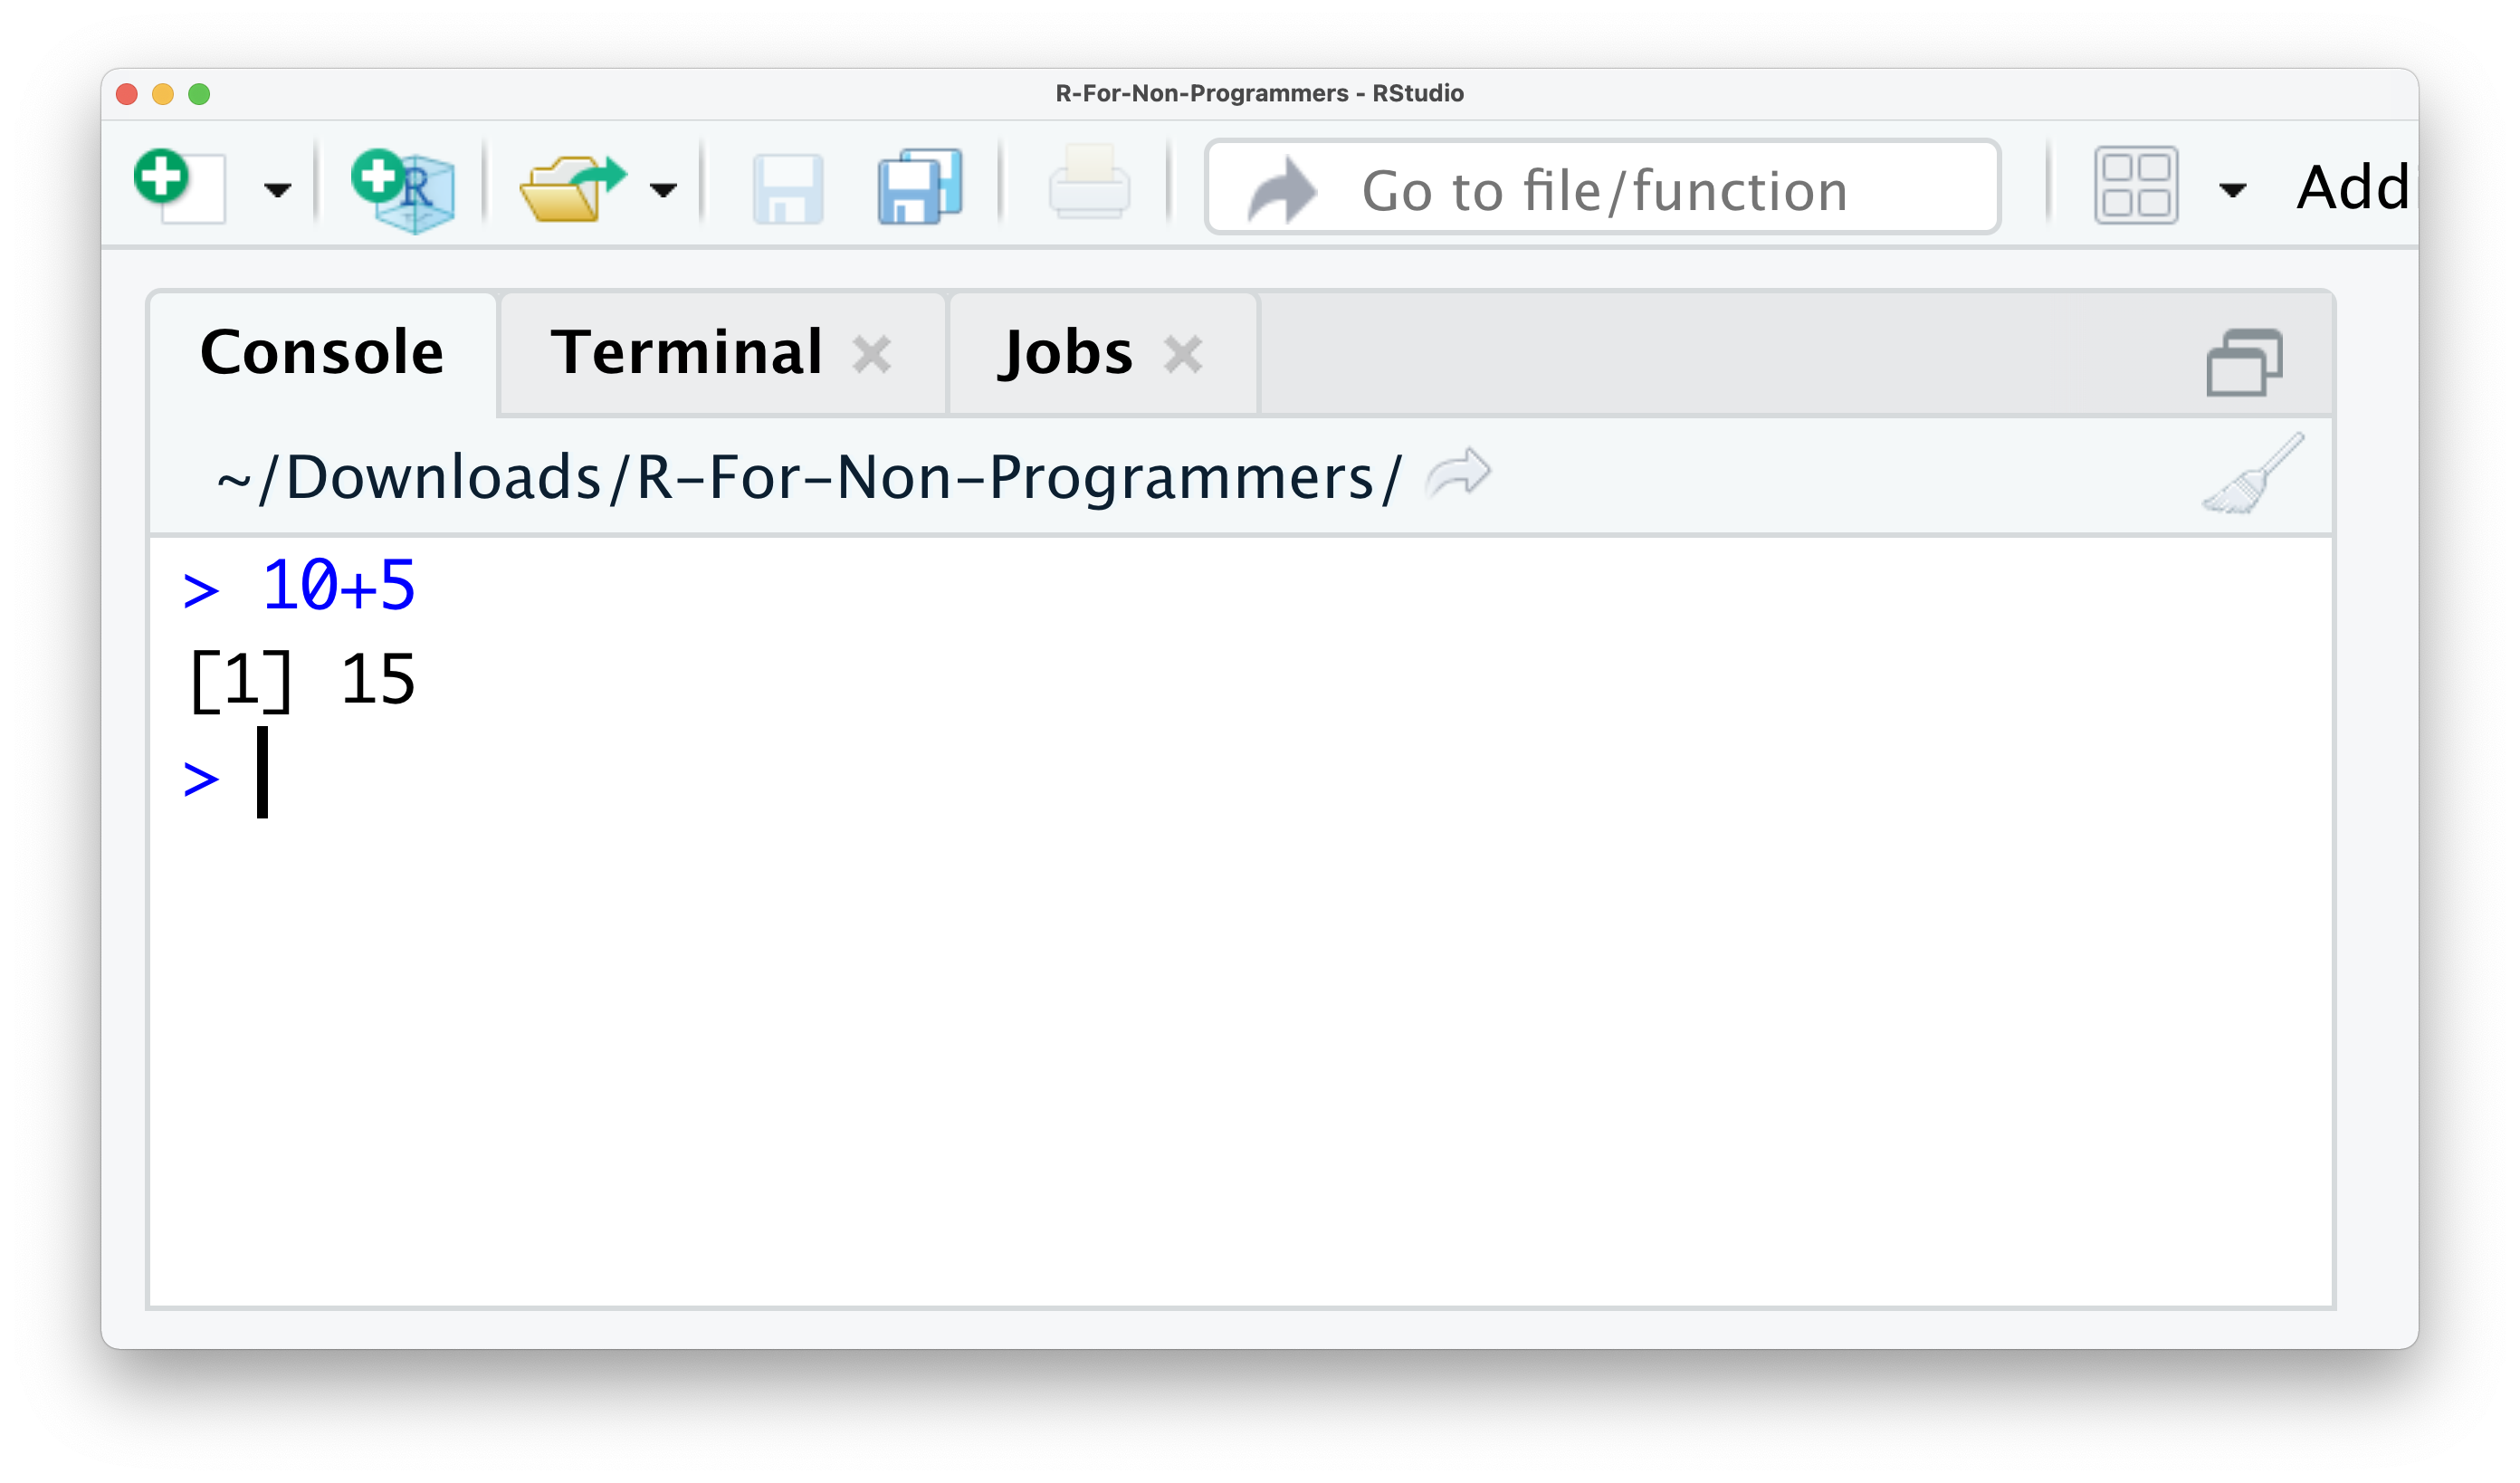
\includegraphics{images/chapter_04_img/02_console_window/console_algebra.png}

You just successfully performed your first successful computation. I
know, this is not quite impressive just yet. \emph{R} is undoubtedly
more than just a giant calculator.

In the top right of the console, you find a symbol that looks like a
broom. This one is quite an important one because it clears your
console. Sometimes the console can become very cluttered and difficult
to read. If you want to remove whatever you computed, you can click the
broom icon and clear the console of all text. I use it so frequently
that I strongly recommend learning the keyboard shortcut, which is
\texttt{Ctrl\ +\ L} on PC and Mac.

\section{The Source window}\label{the-source-window}

In the top left, you can find the source window. The term `source' can
be understood as any type of file, e.g.~data, programming code, notes,
etc. The source panel can fulfil many functions, such as:

\begin{itemize}
\item
  Inspect data in an Excel-like format (see also Chapter
  @ref(import-your-data))
\item
  Open programming code, e.g.~an R Script (see Chapter
  @ref(creating-an-r-script))
\item
  Open other text-based file formats, e.g.

  \begin{itemize}
  \item
    Plain text (.txt),
  \item
    Markdown (.md),
  \item
    Websites (.html),
  \item
    LaTeX (.tex),
  \item
    BibTex (.bib),
  \end{itemize}
\item
  Edit scripts with code in it,
\item
  Run the analysis you have written.
\end{itemize}

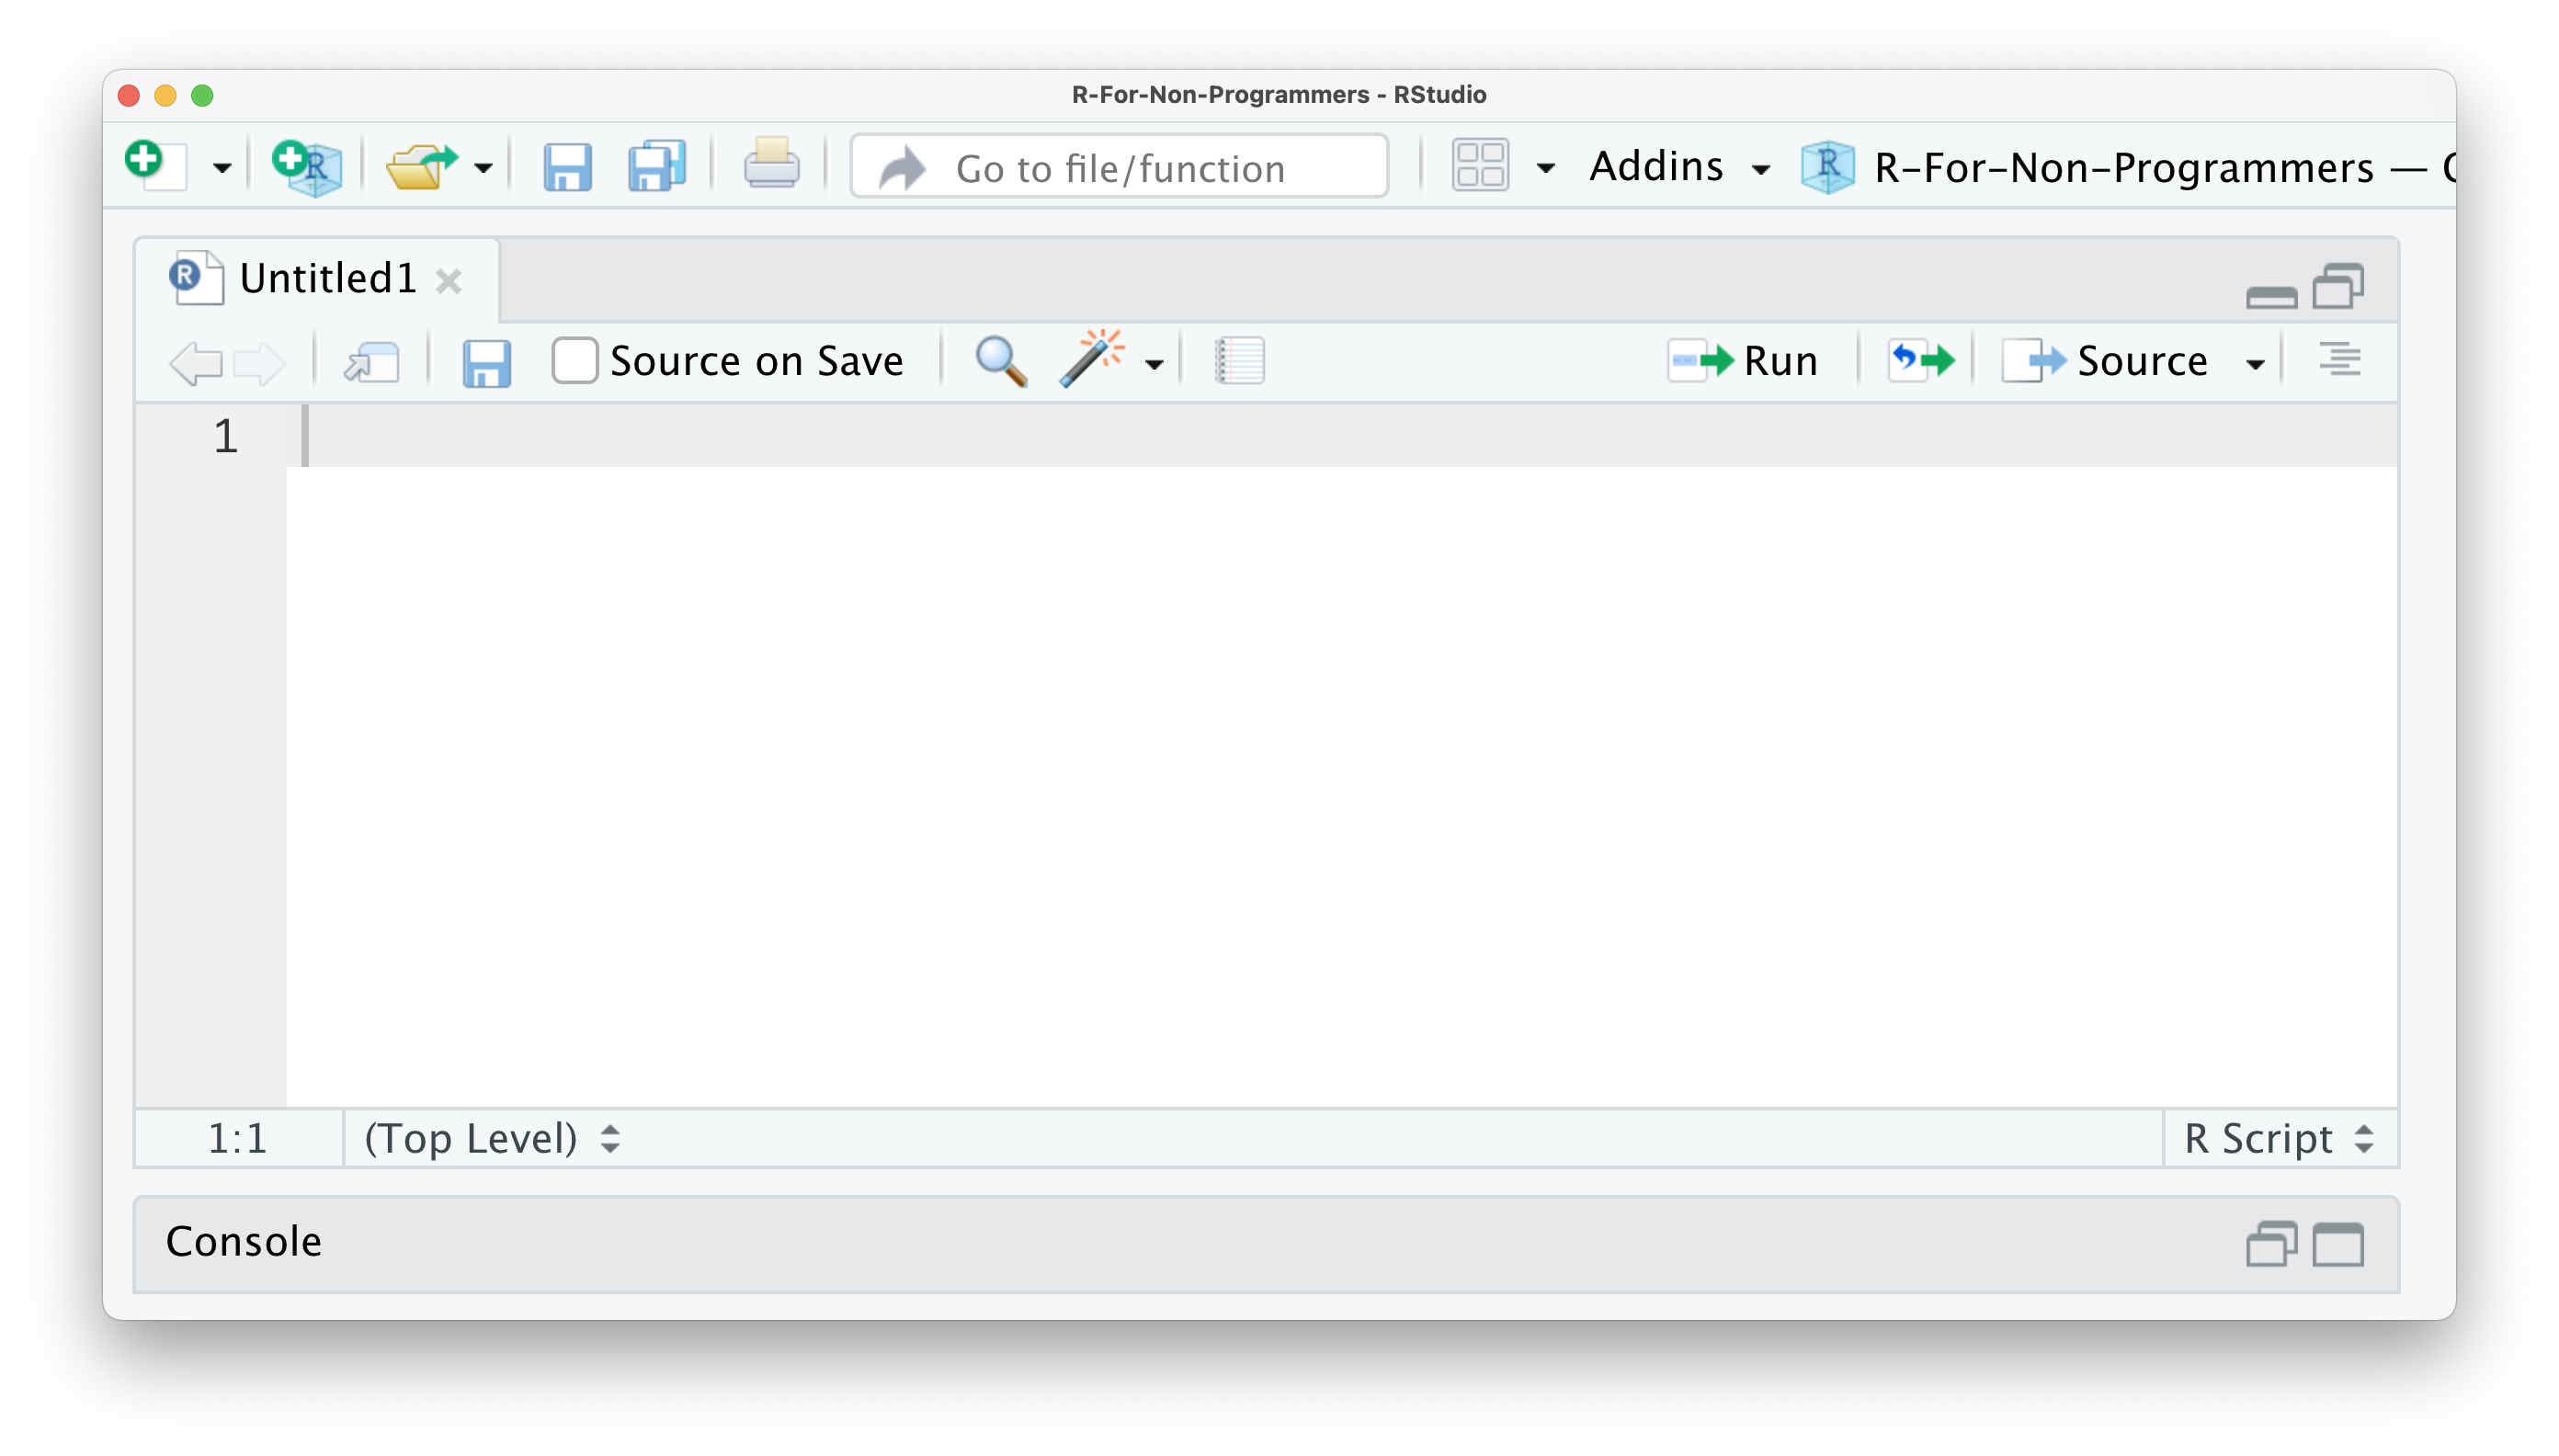
\includegraphics{images/chapter_04_img/03_source_window/01_rstudio_source.png}

In other words, the source window will show you whatever file you are
interested in, as long as RStudio can read it - and no, Microsoft Office
Documents are not supported. Another limitation of the source window is
that it can only show text-based files. So opening images, etc. would
not work.

\section{The Environment / History / Connections / Tutorial
window}\label{the-environment-history-connections-tutorial-window}

The window in the top right shows multiples panes. The first pane is
called \emph{Environment} and shows you objects which are available for
computation. One of the first objects you will create is your dataset
because, without data, we cannot perform any analysis. Another object
could be a plot showing the number of male and female participants in
your study. To find out how to create objects yourself, you can take a
glimpse at it (see Chapter @ref(inspecting-raw-data)). Besides datasets
and plots, you will also find other objects here, e.g.~lists, vectors
and functions you created yourself. Don't worry if none of these words
makes sense at this point. We will cover each of them in the upcoming
chapters. For now, remember this is a place where you can find different
objects you created.

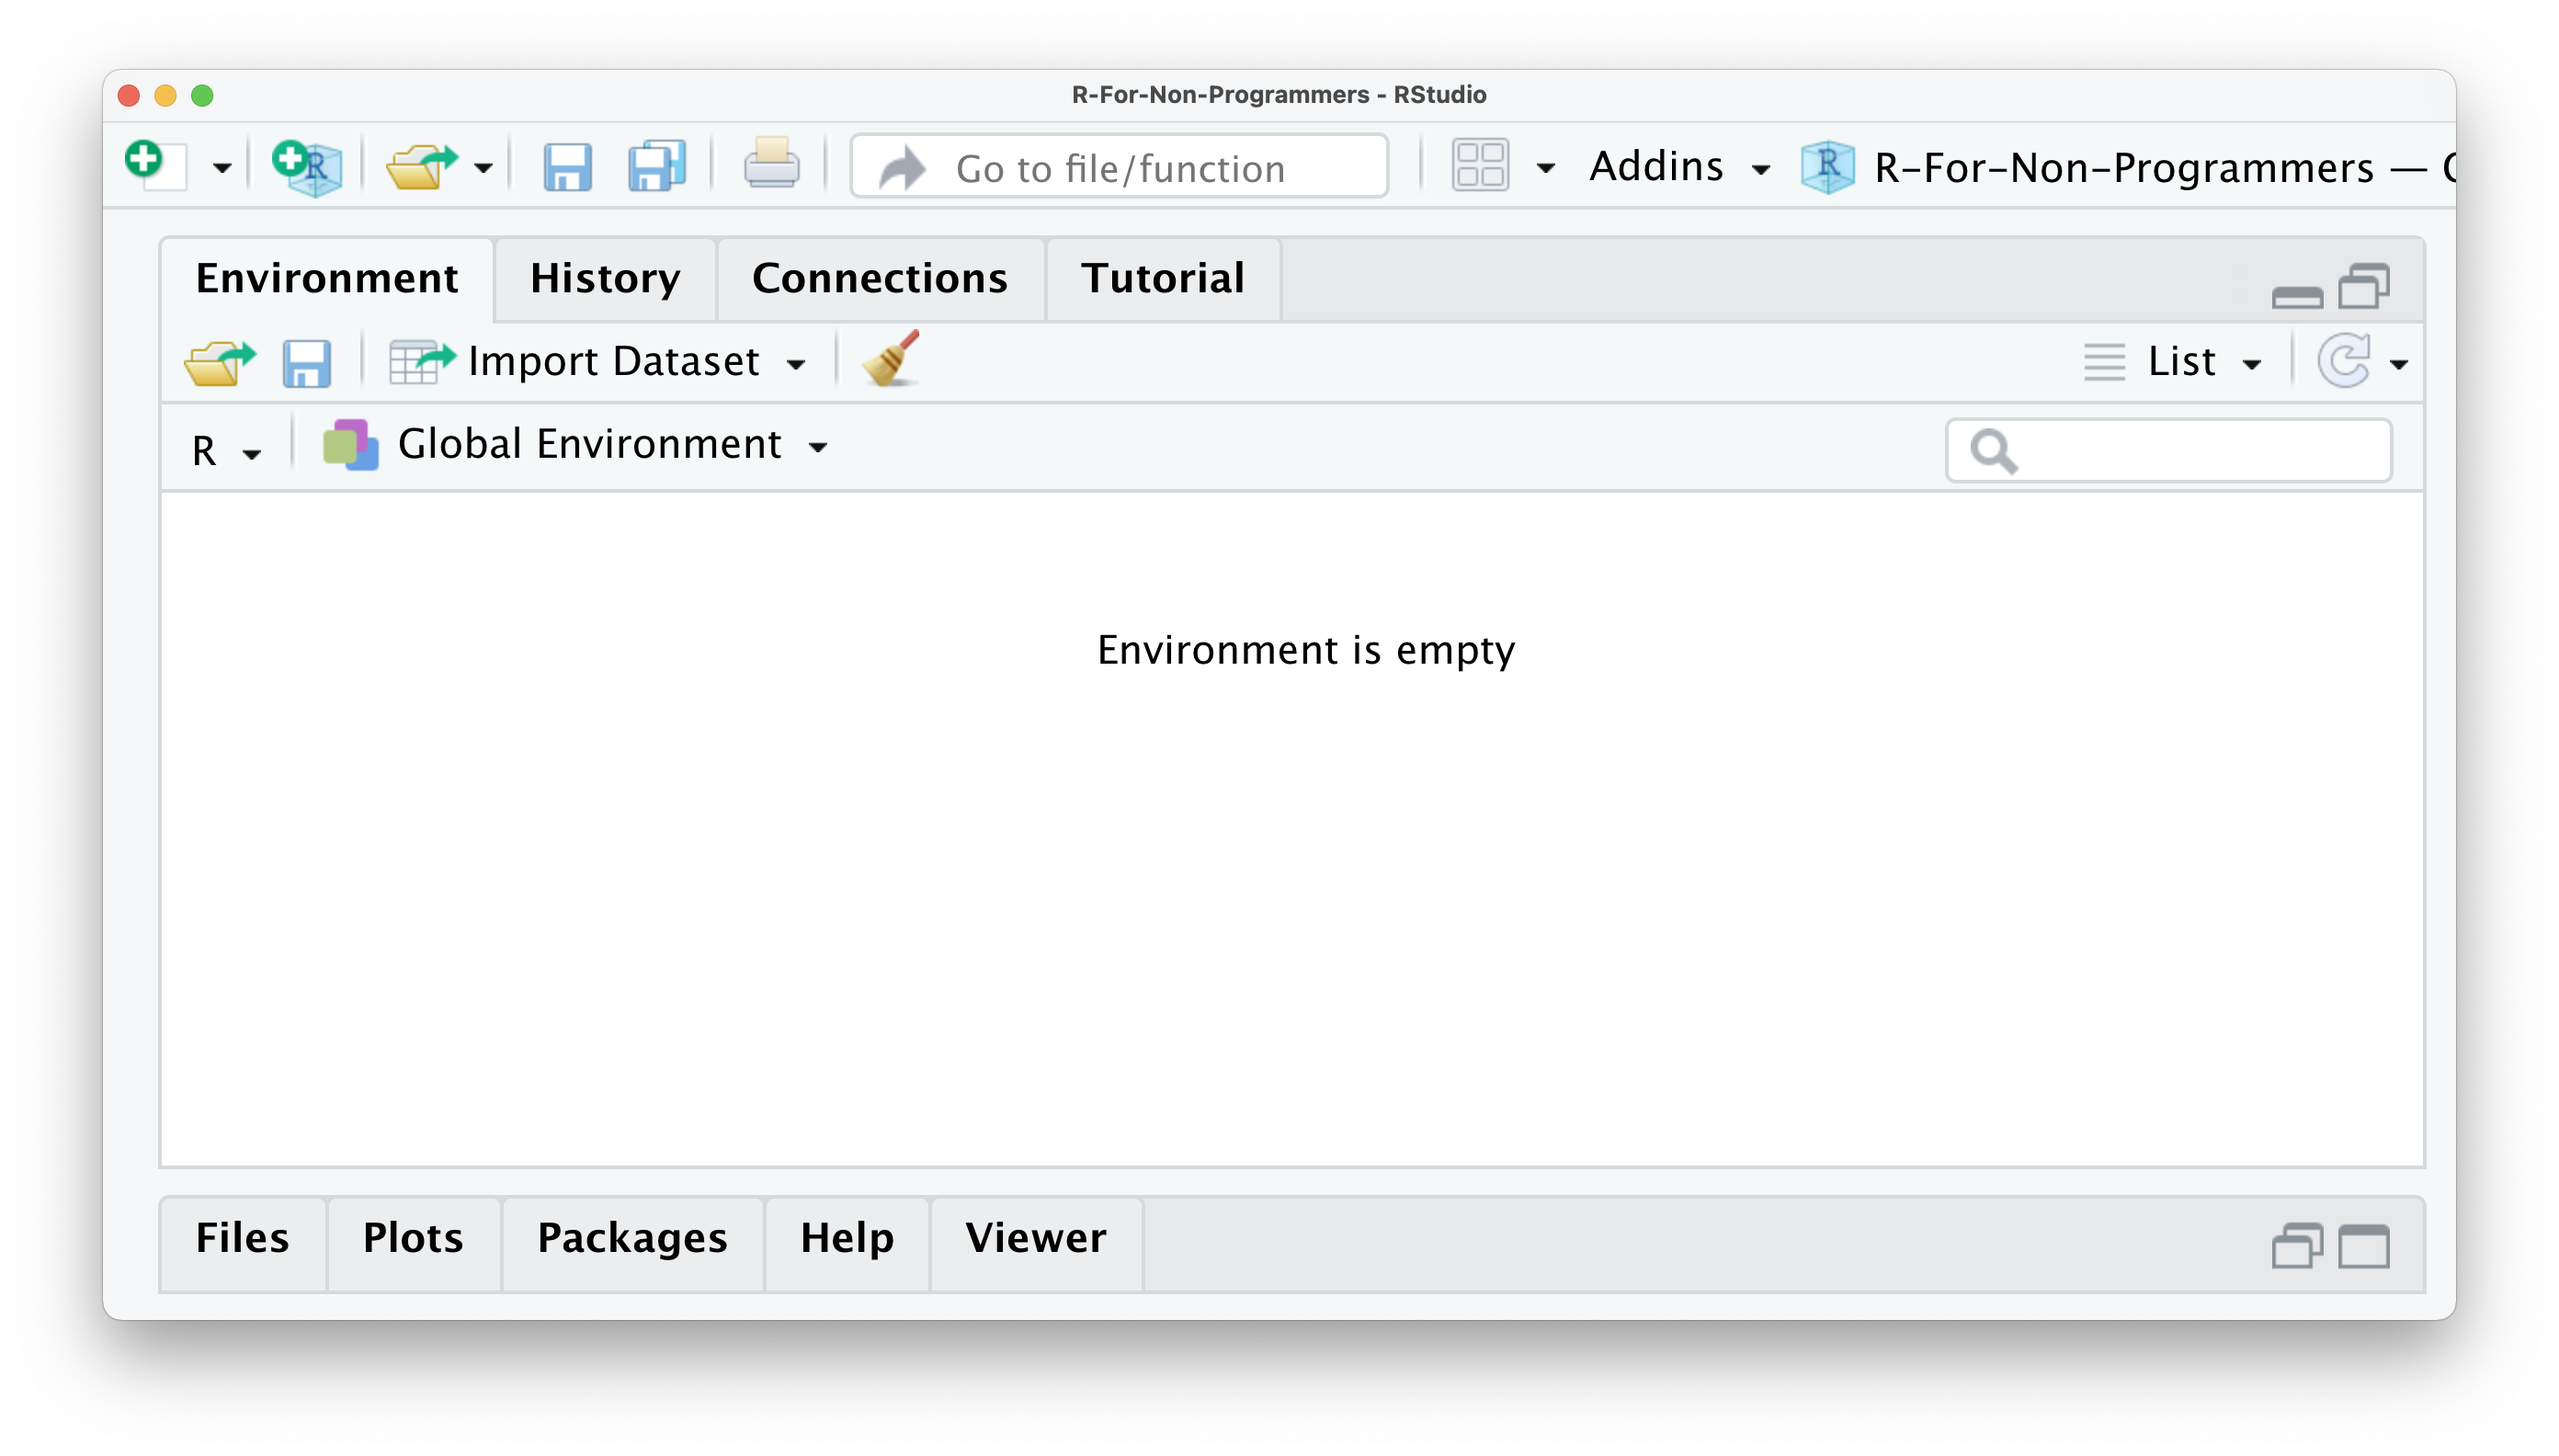
\includegraphics{images/chapter_04_img/04_environment_history_etc/01_rstudio_environment.png}

The \emph{History} pane is very easy to understand. Whatever computation
you run in the console will be stored. So you can go back and see what
you coded and rerun that code. Remember the example from above where we
computed the sum of \texttt{10+5}? This computation is stored in the
history of RStudio, and you can rerun it by clicking on \texttt{10+5} in
the history pane and then click on \texttt{To\ Console}. This will
insert \texttt{10+5} back into the console, and we can hit
\texttt{Return\ ↵} to retrieve the result. You also have the option to
copy the code into an existing or new \emph{R} Script by clicking on
\texttt{To\ Source}. By doing this, you can save this computation on
your computer and reuse it later. Finally, if you would like to store
your history, you can do so by clicking on the
\texttt{floppy\ disk\ symbol}. There are two more buttons in this pane,
one allows you to delete individual entries in the history (the white
page with the red circle on it), and the last one, a \texttt{broom},
clears the entire history (irrevocably).

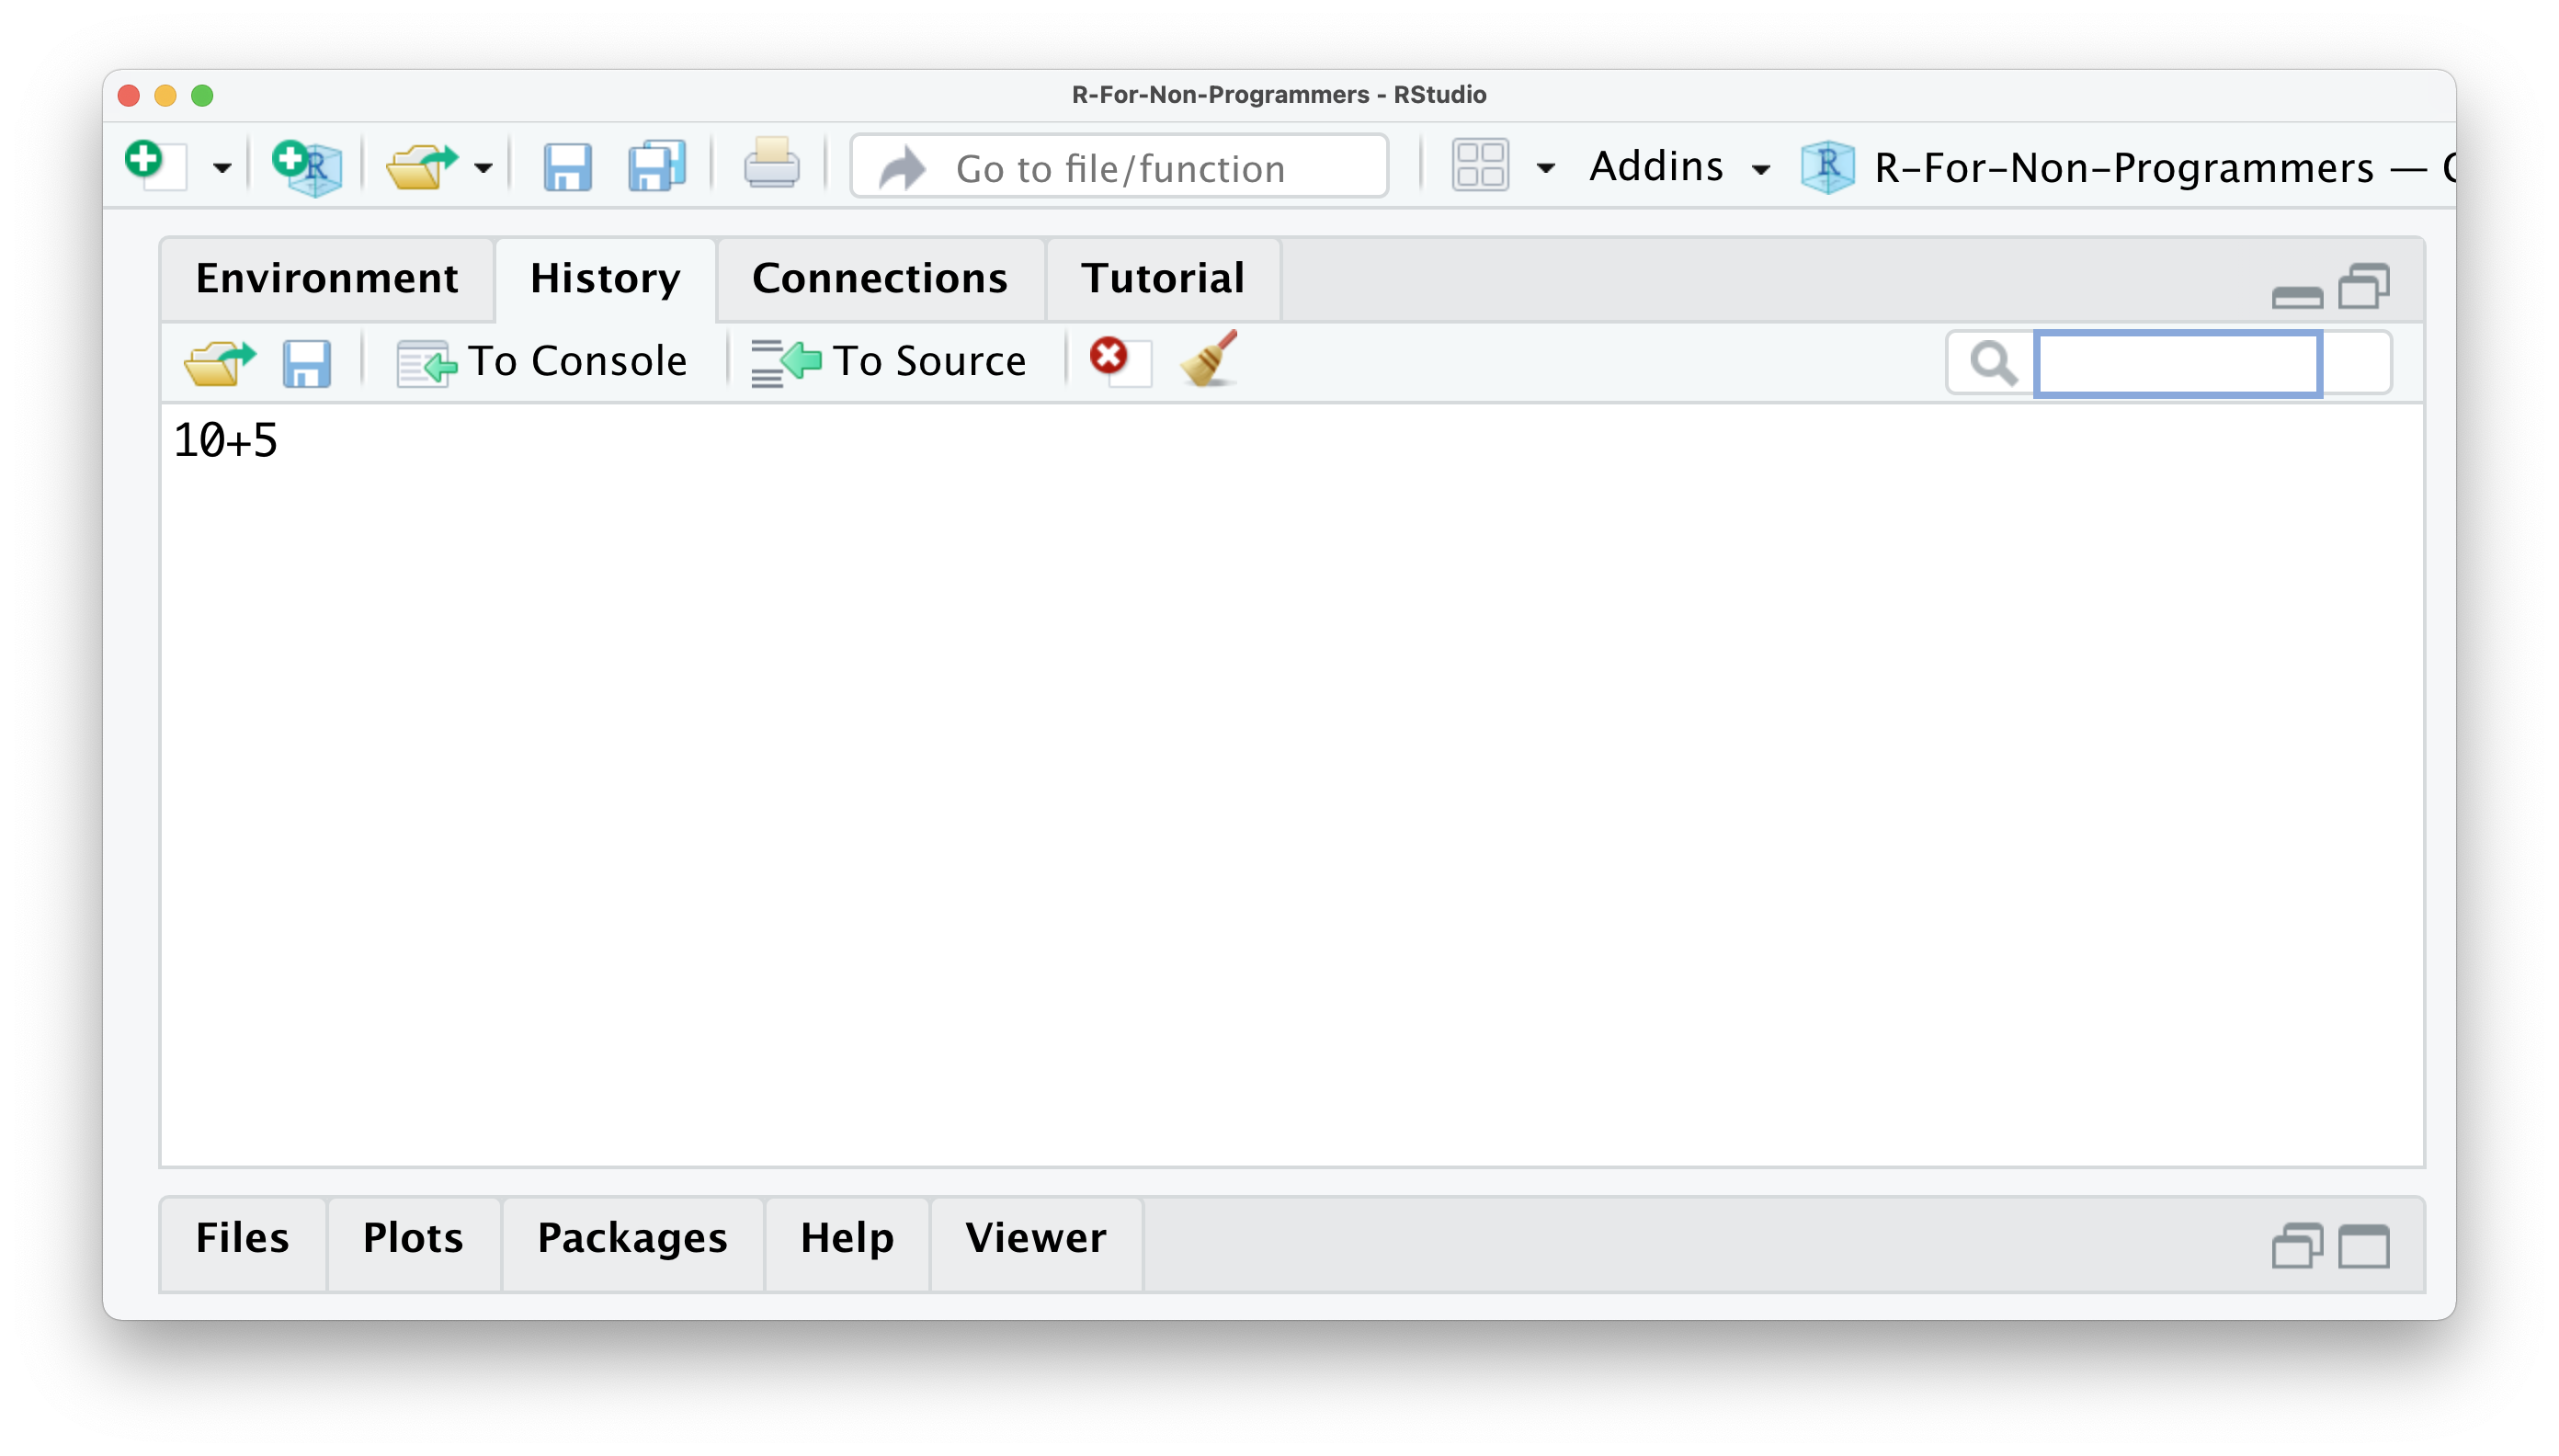
\includegraphics{images/chapter_04_img/04_environment_history_etc/02_rstudio_history.png}

The pane \emph{Connections} allows you to tab into external databases
directly. This can come in handy when you work collaboratively on the
same data or want to work with extensive datasets without having to
download them. However, for an introduction to \emph{R}, we will not use
this feature of RStudio.

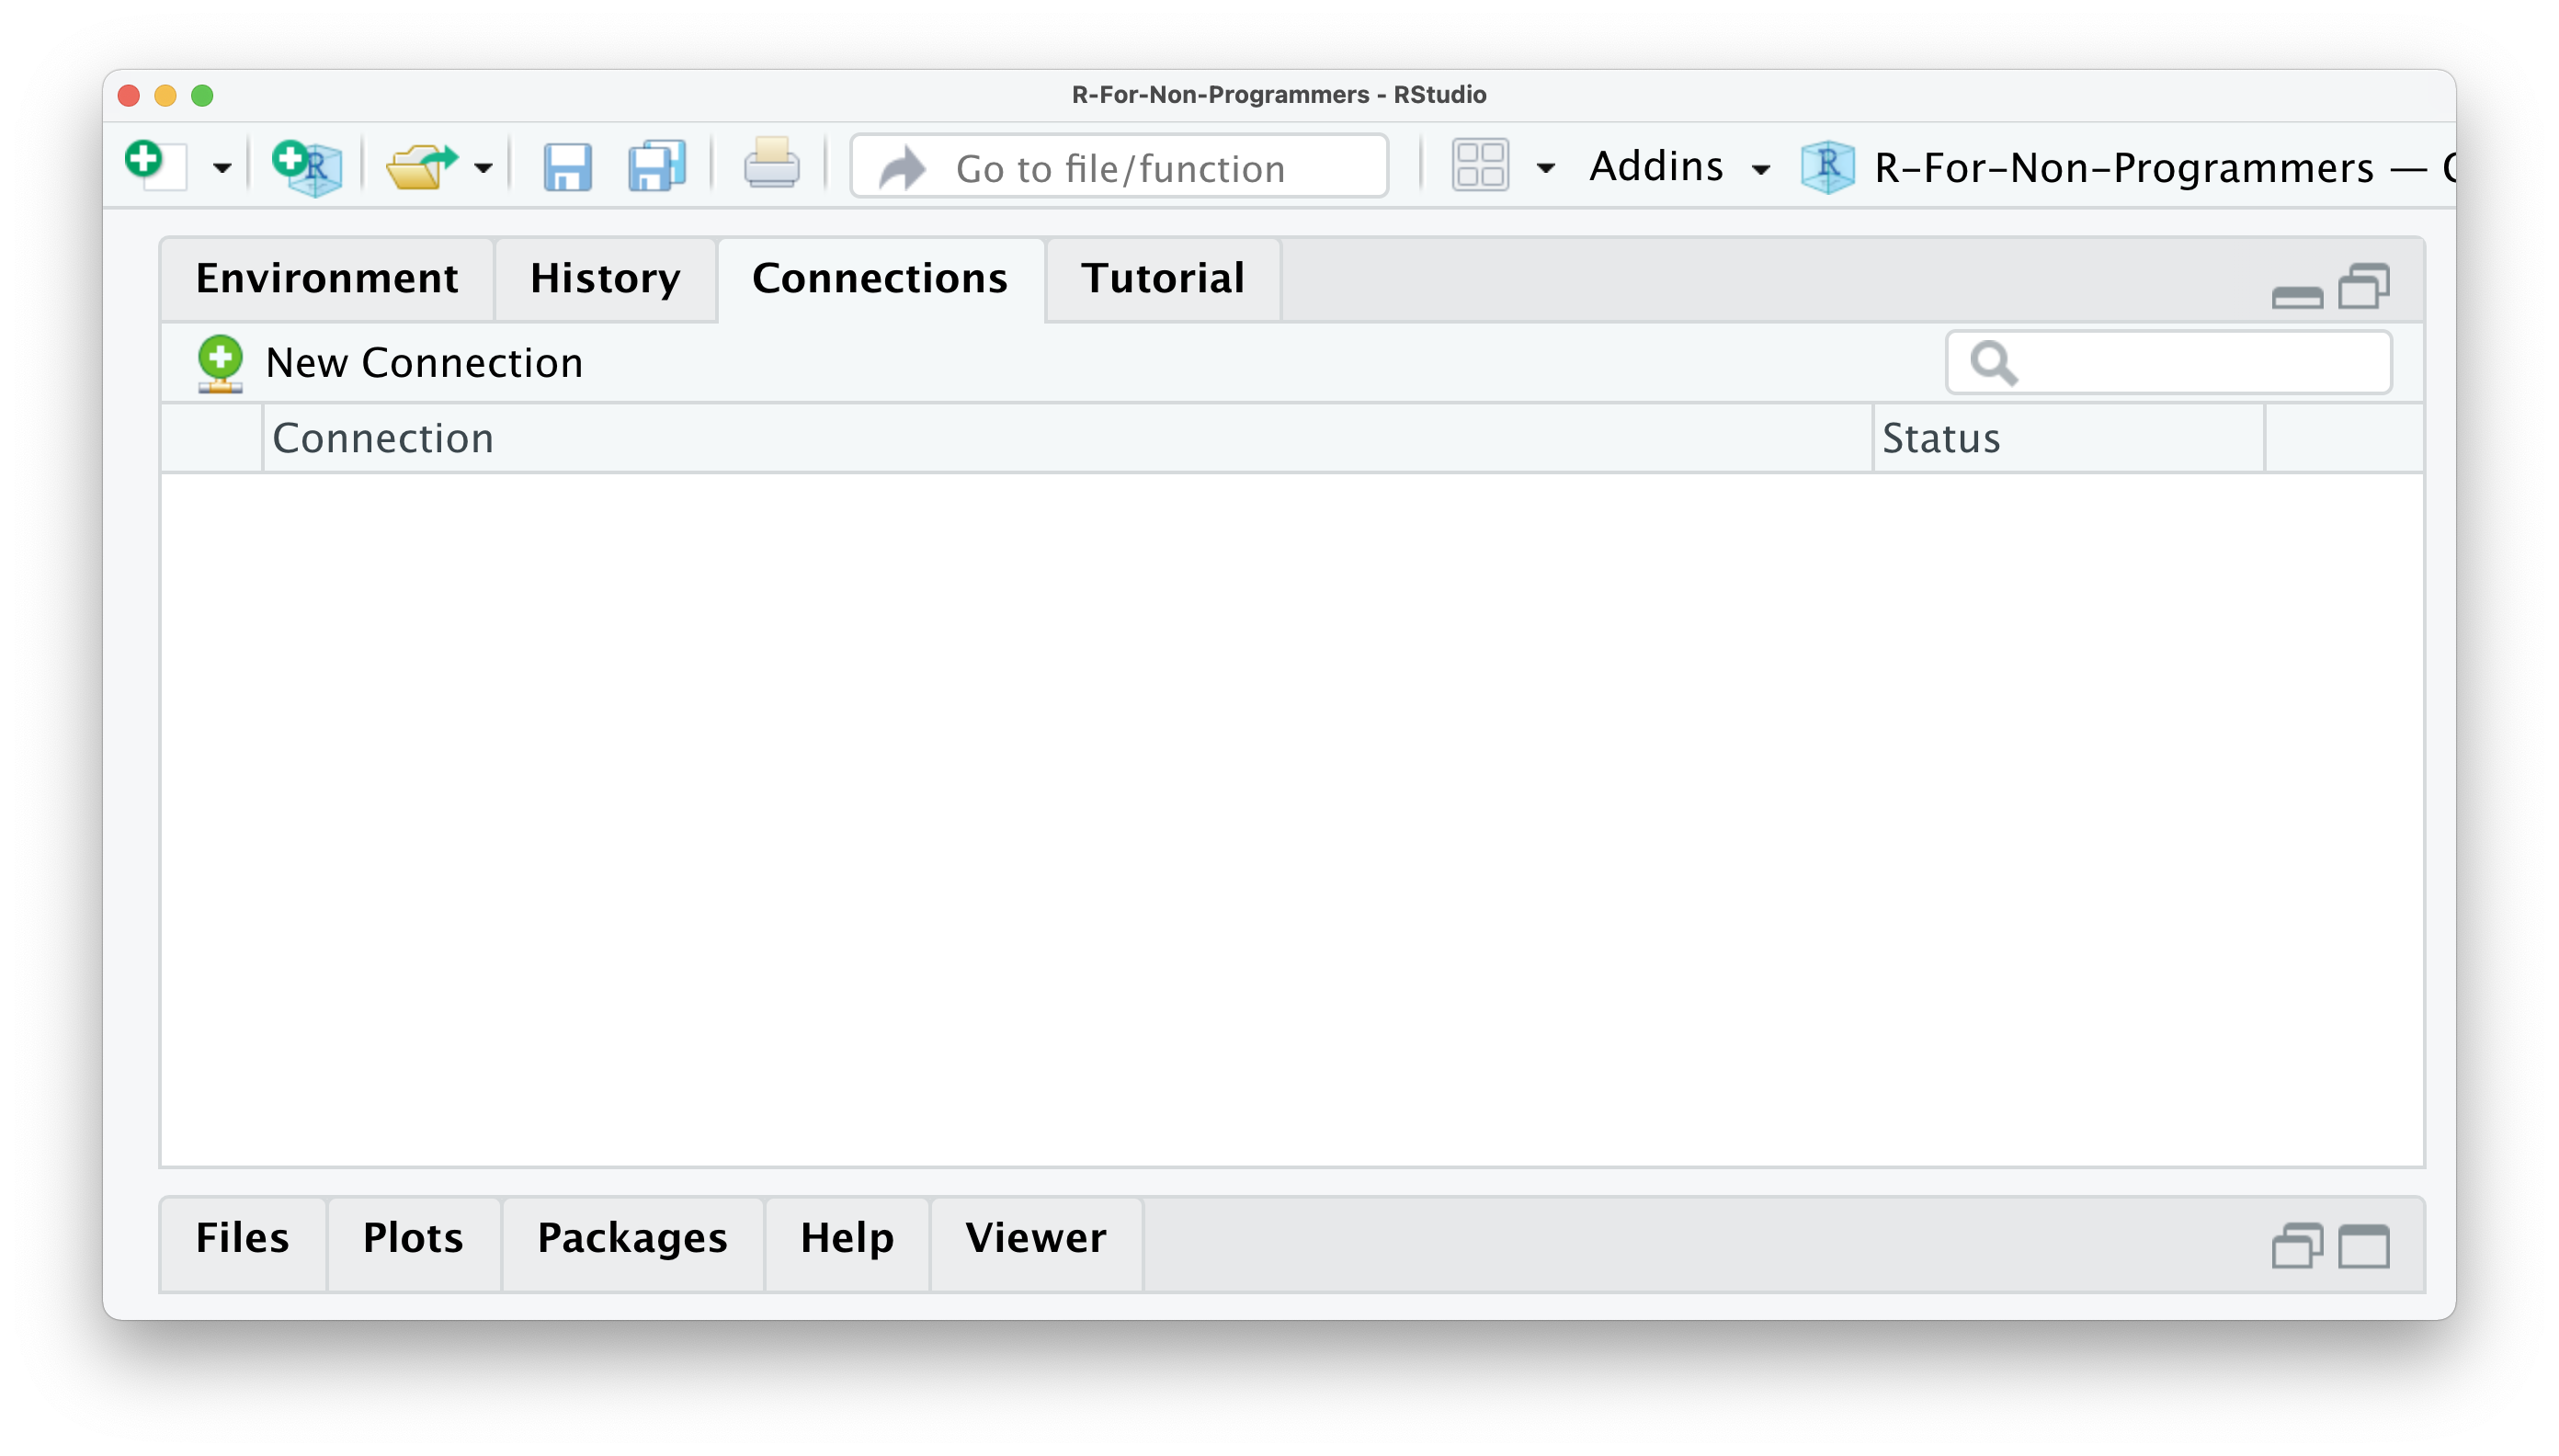
\includegraphics{images/chapter_04_img/04_environment_history_etc/03_rstudio_connections.png}

The last pane is called \emph{Tutorial}. Here you can find additional
materials to learn \emph{R} and RStudio. If you search for more great
content to learn \emph{R}, this serves as a great starting point.

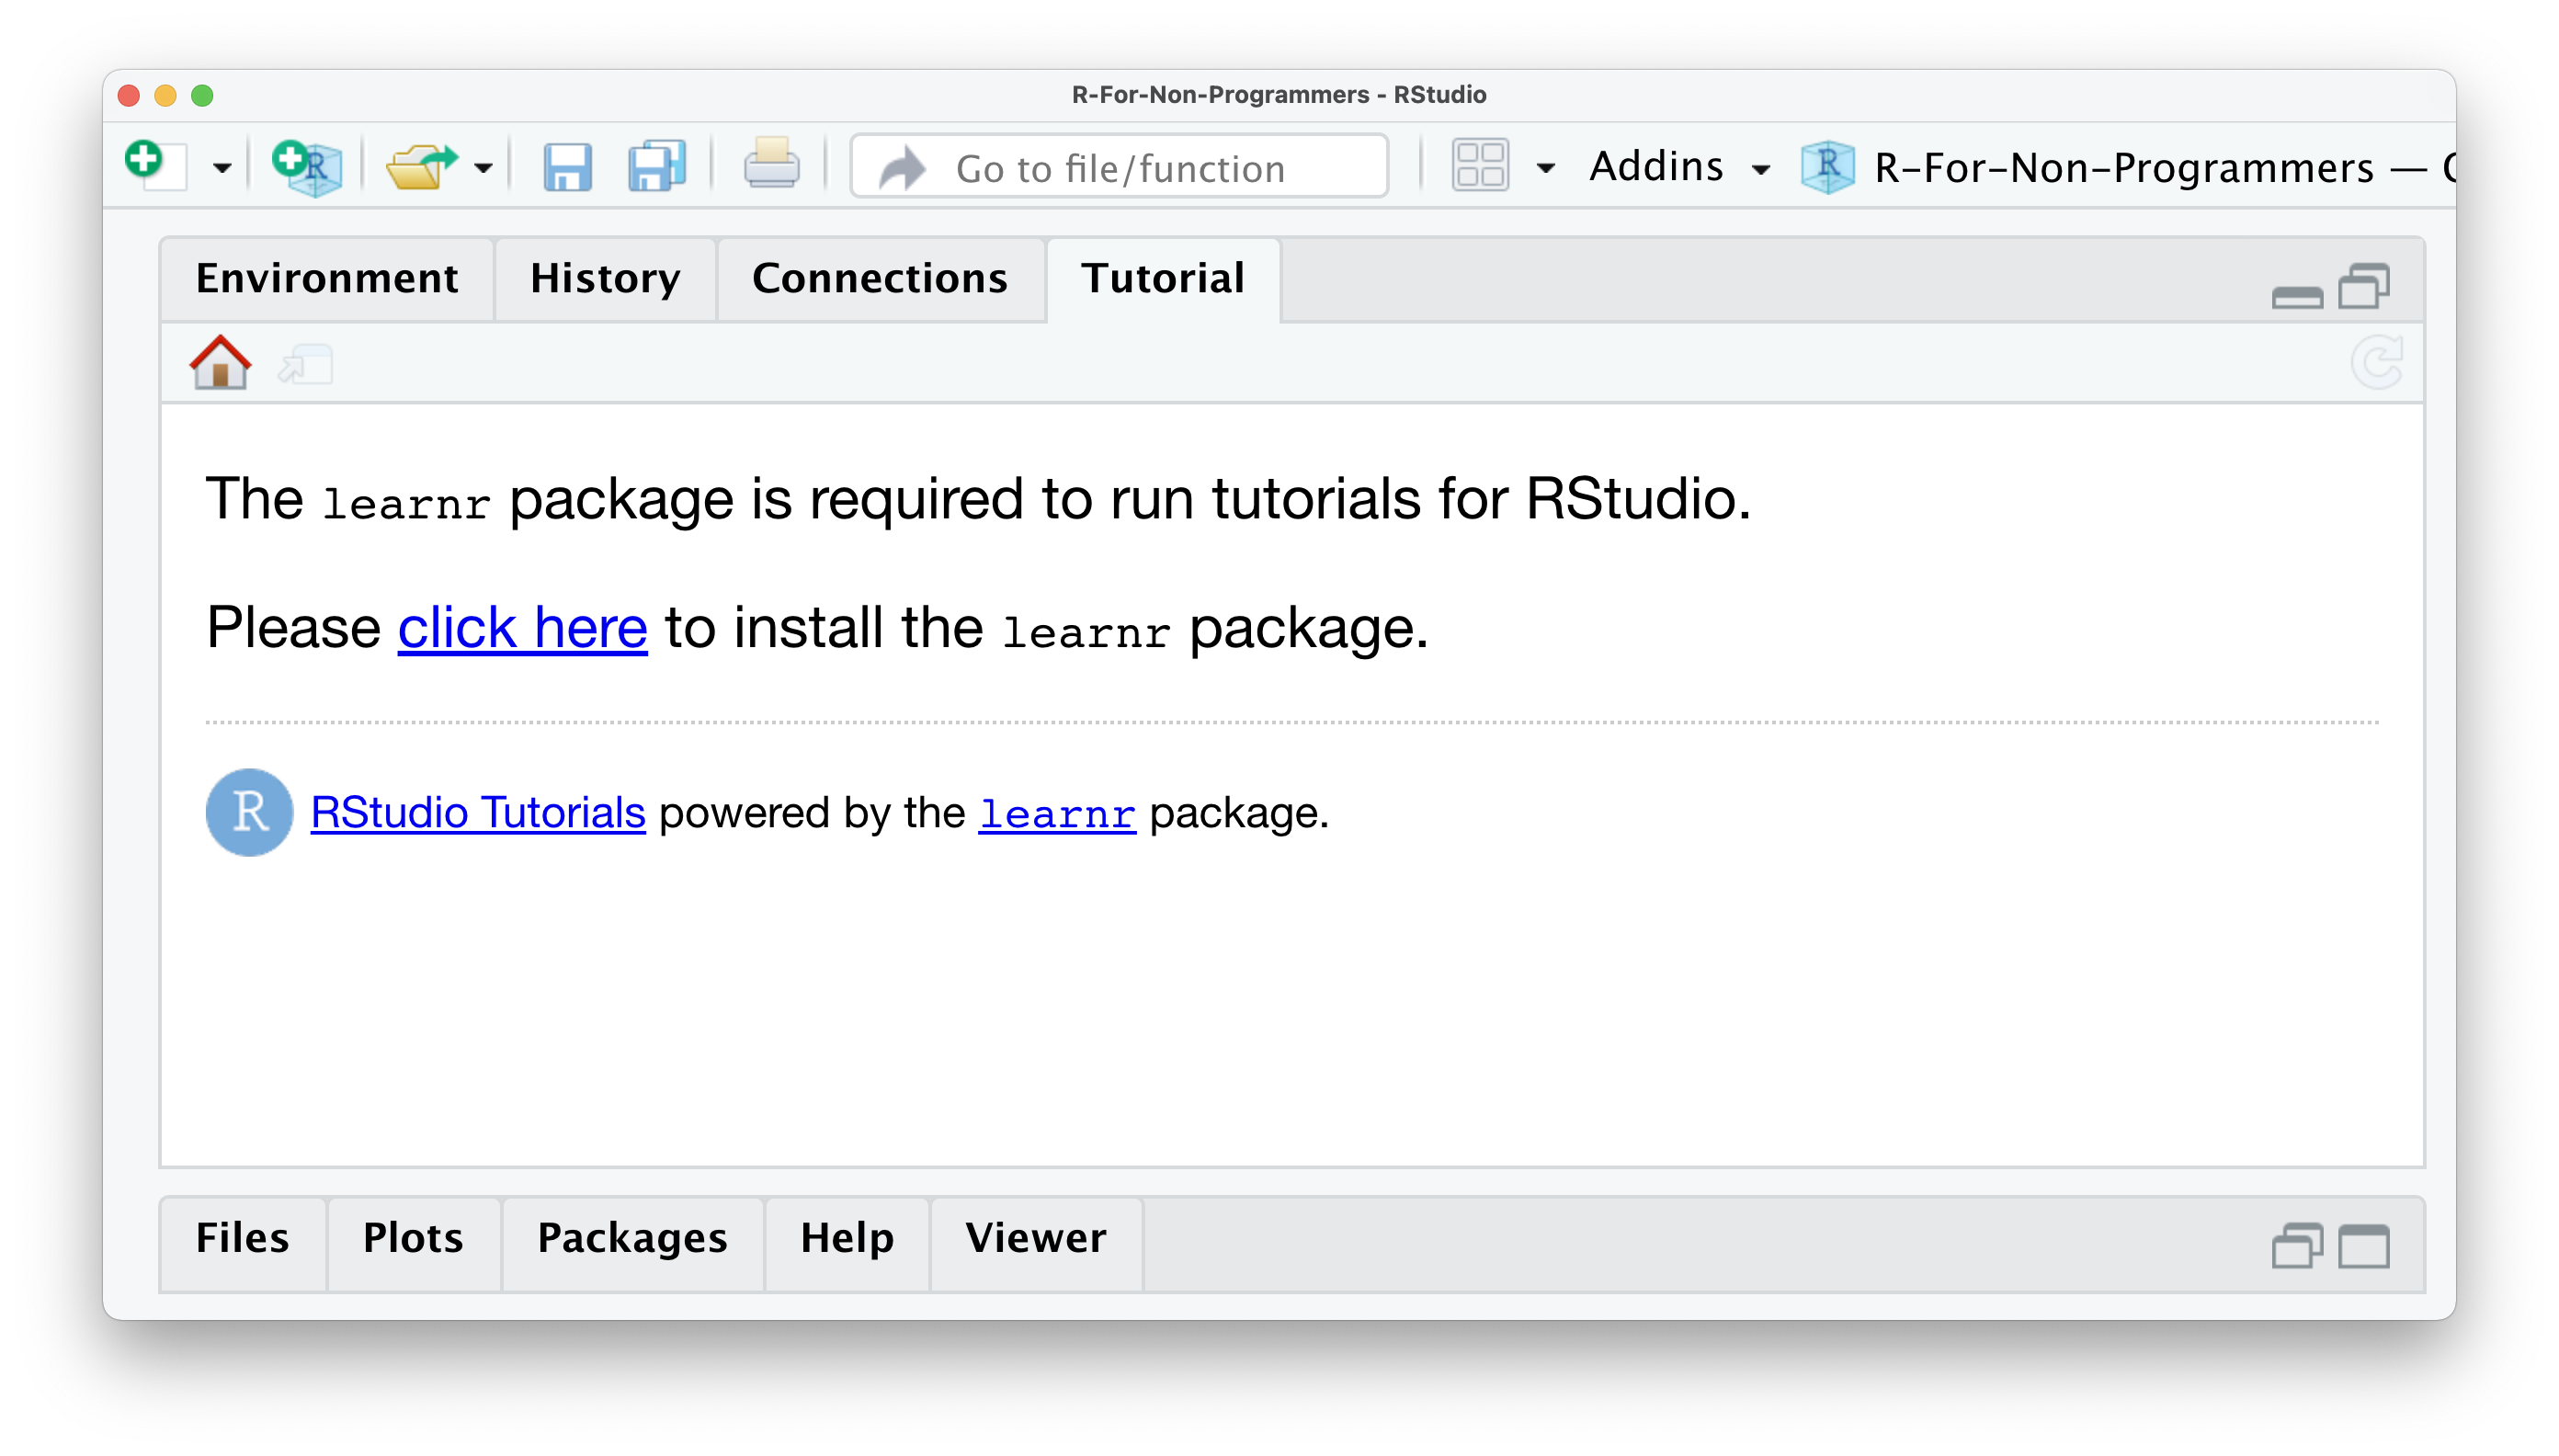
\includegraphics{images/chapter_04_img/04_environment_history_etc/04_rstudio_tutorial.png}

\section{The Files / Plots / Packages / Help / Viewer
window}\label{the-files-plots-packages-help-viewer-window}

The last window consists of five essential panes. The first one is the
\emph{Files} pane. As the name indicates, it lists all the files and
folders in your root directory. A root directory is the default
directory where RStudio saves your files, for example, your analysis.
However, we will look at how you can properly set up your projects in
RStudio in Chapter @ref(starting-your-r-projects). Thus, the
\emph{Files} pane is an easy way to load data into RStudio and create
folders to keep your research project well organised.

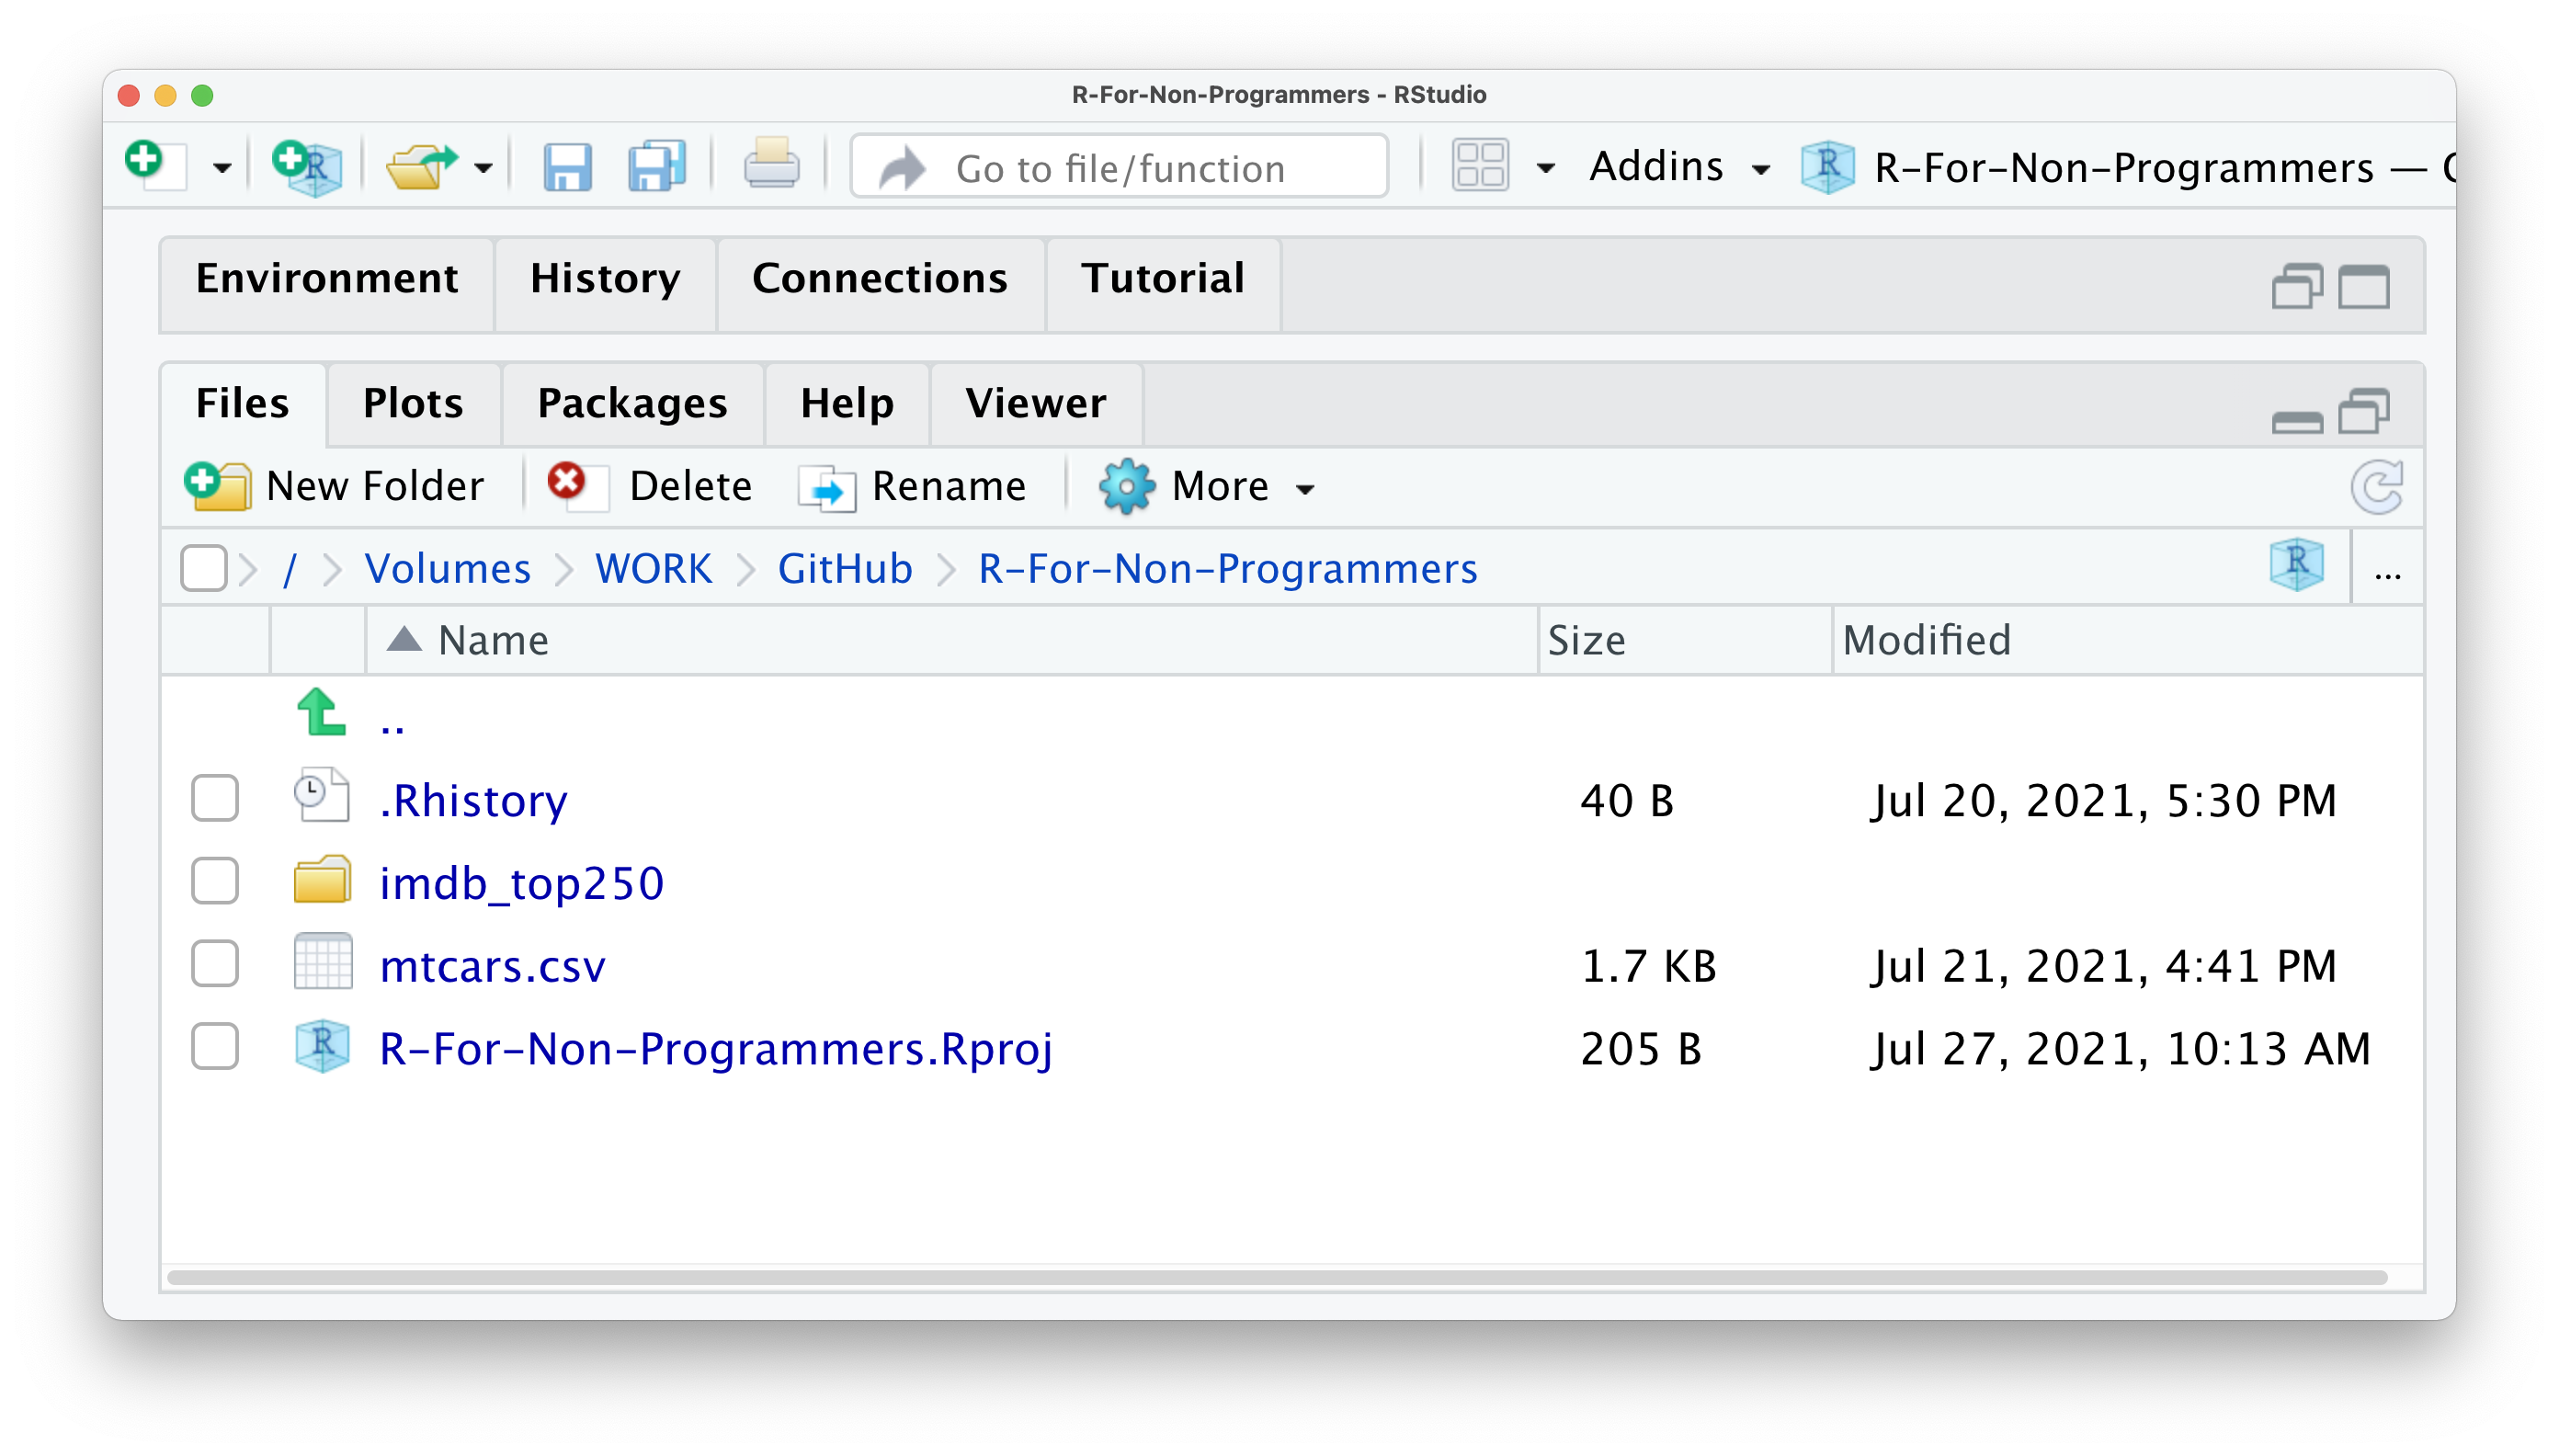
\includegraphics{images/chapter_04_img/05_files_plots_etc/01_rstudio_files.png}

Since the Console cannot reproduce data visualisations, RStudio offers a
way to do this very easily. It is through the \emph{Plots} pane. This
pane is exclusively designed to show you any plots you have created
using \emph{R}. Here is a simple example that you can try. Type into
your console \texttt{boxplot(mtcars\$hp)}.

\begin{Shaded}
\begin{Highlighting}[]
\CommentTok{\# Here we create a nice boxplot using a dataset called \textquotesingle{}mtcars\textquotesingle{}}
\FunctionTok{boxplot}\NormalTok{(mtcars}\SpecialCharTok{$}\NormalTok{hp)}
\end{Highlighting}
\end{Shaded}

\begin{figure}[H]

\centering{

\captionsetup{labelsep=none}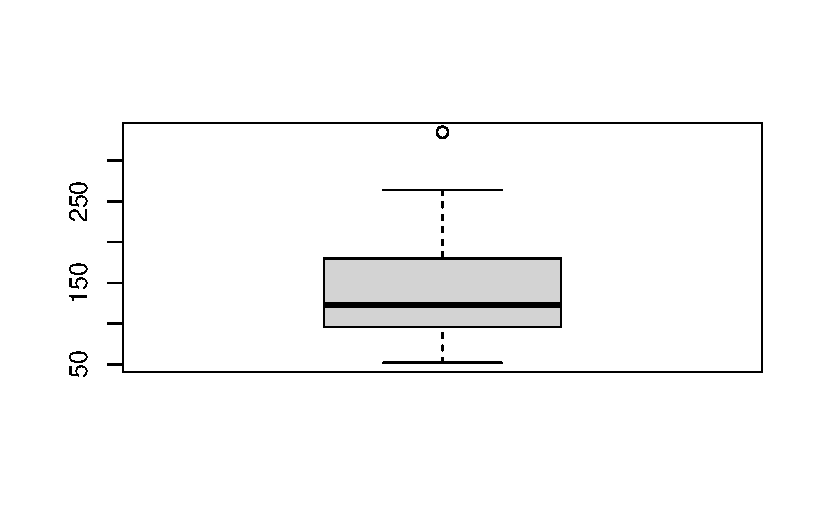
\includegraphics{04_rstudio_interface_files/figure-pdf/fig-simple-boxplot-1.pdf}

}

\caption{\label{fig-simple-boxplot}}

\end{figure}%

Although this is a short piece of coding, it performs quite a lot of
steps:

\begin{itemize}
\item
  it uses a function called \texttt{boxplot()} to draw a boxplot of
\item
  a variable called \texttt{hp} (for horsepower), which is located in
\item
  a dataset named \texttt{mtcars},
\item
  and it renders the graph in your \emph{Plots} pane
\end{itemize}

This is how the plot should look like in your RStudio \emph{Plots} pane.

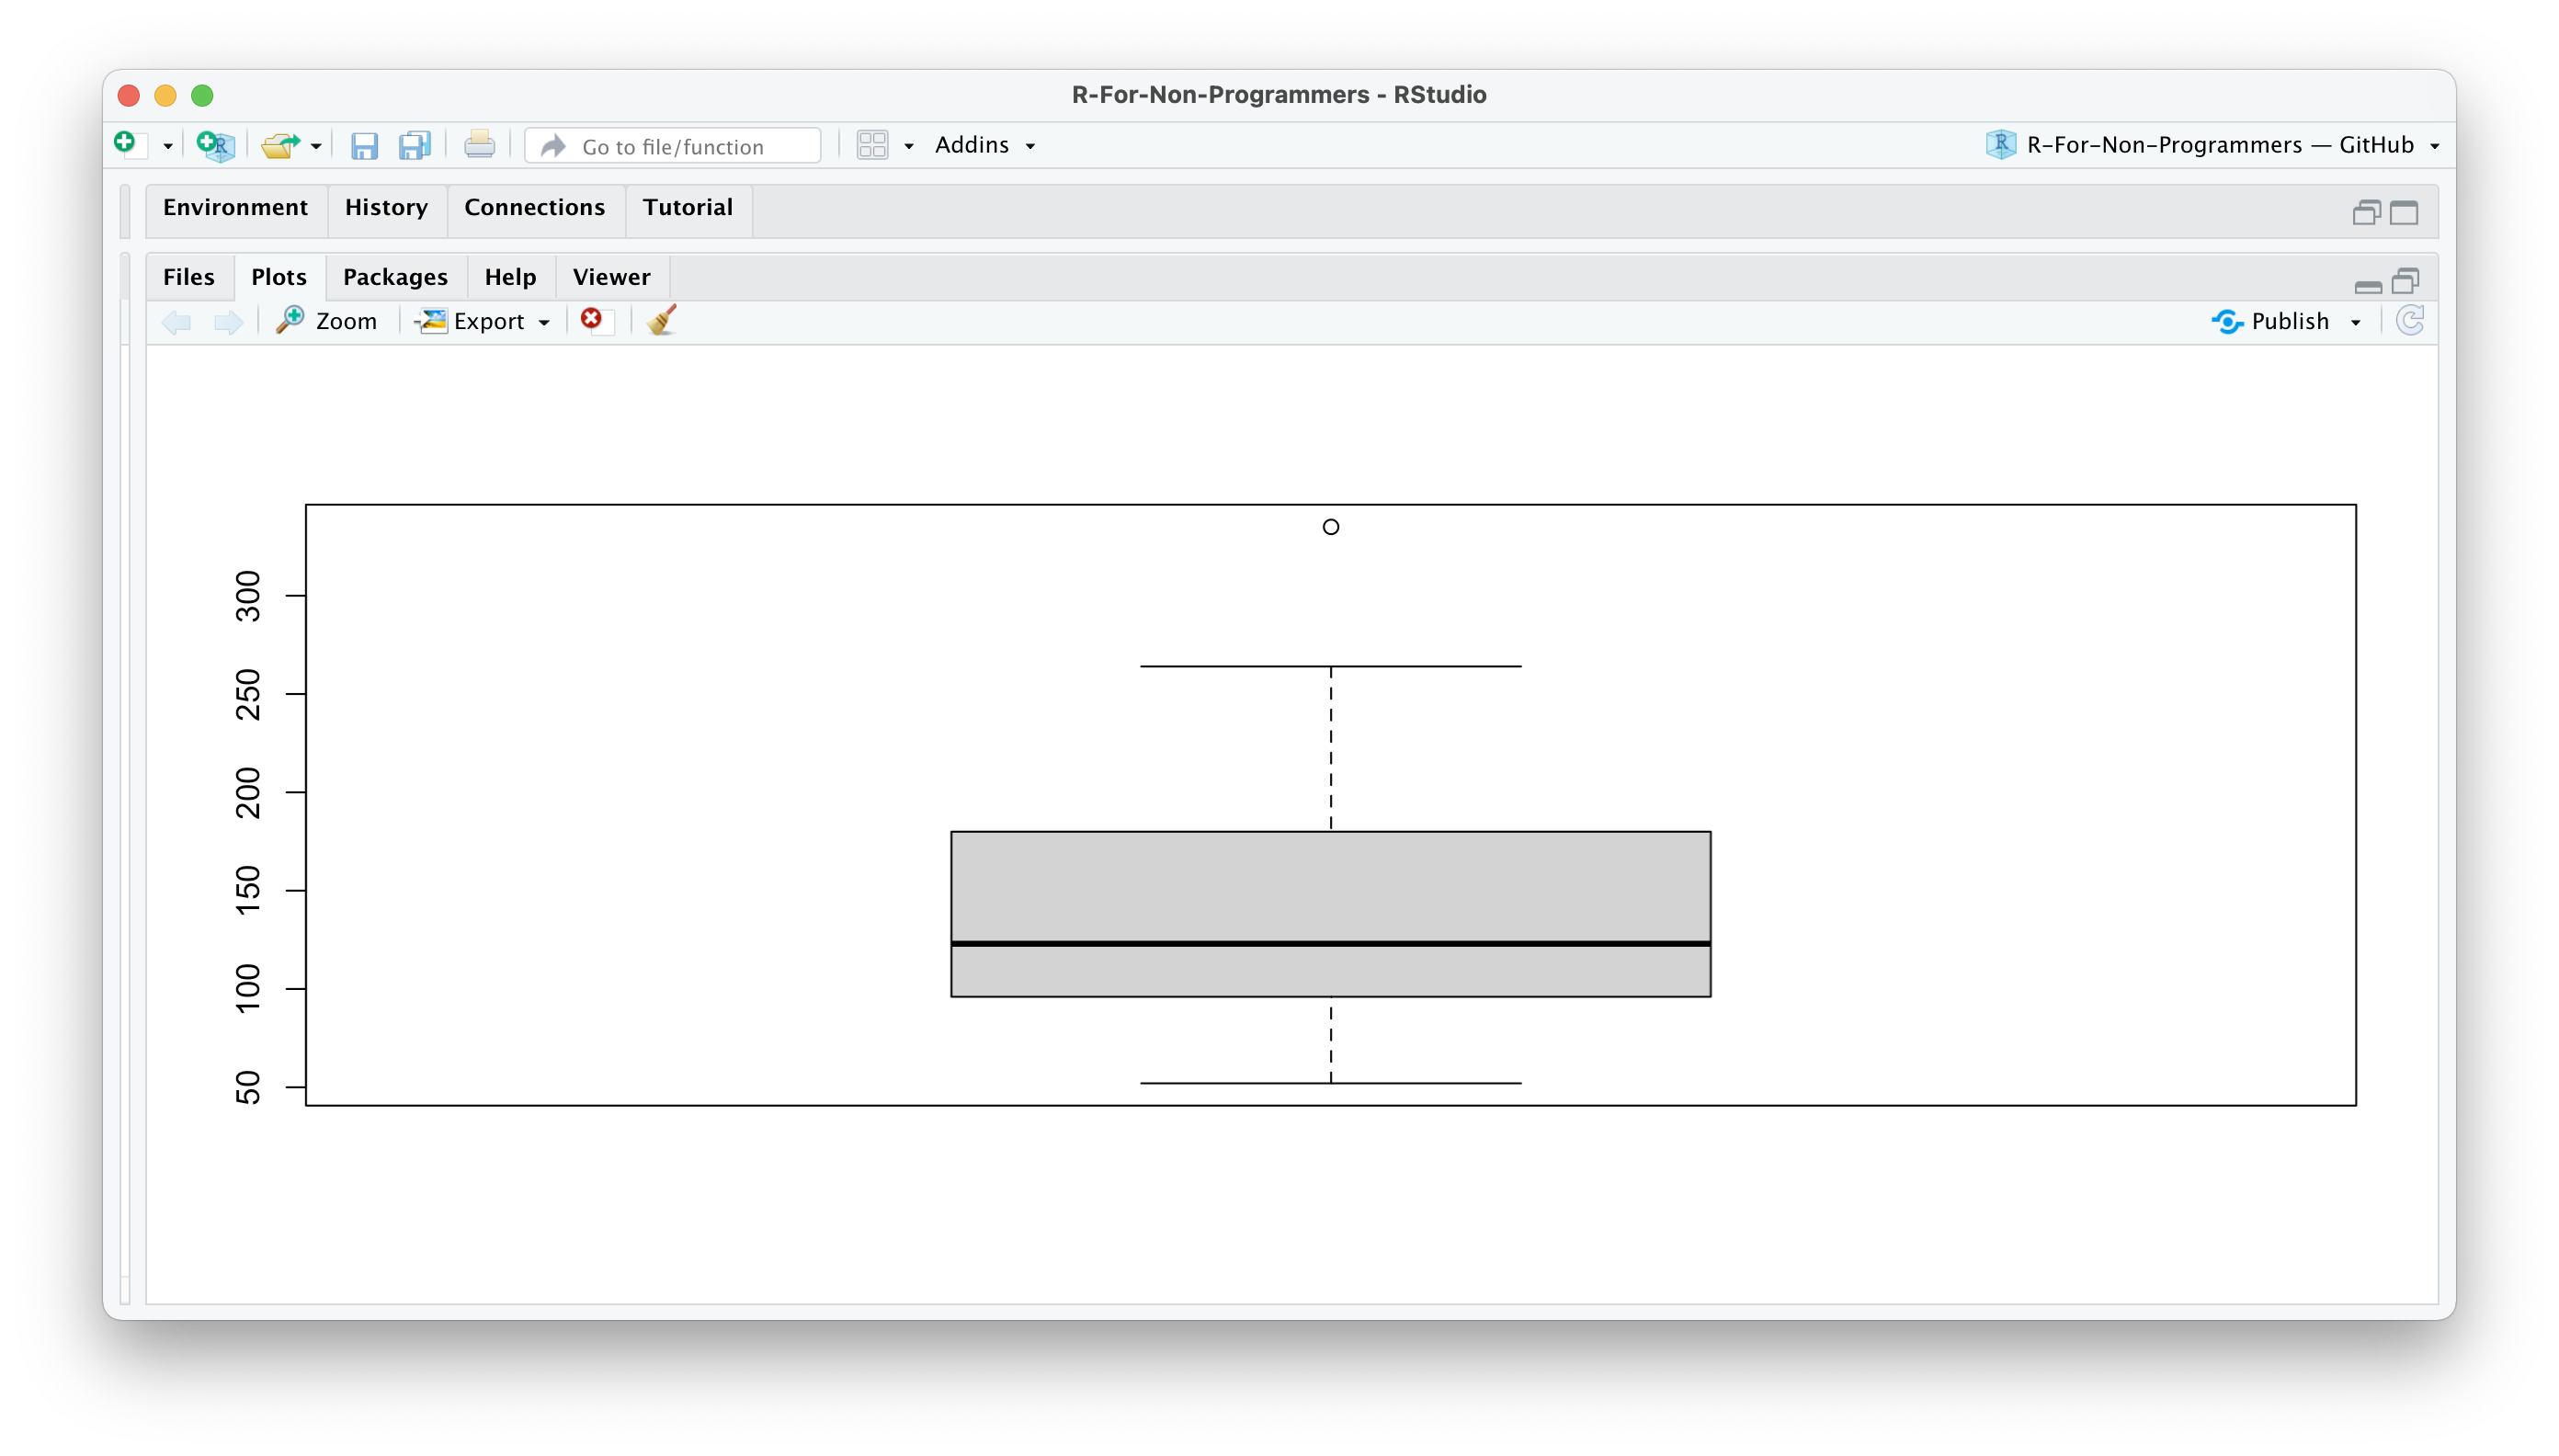
\includegraphics{images/chapter_04_img/05_files_plots_etc/02_rstudio_plots.png}

If you wish to delete the plot, you can click on the
\texttt{red\ circle\ with\ a\ white\ x} symbol. This will delete the
currently visible plot. If you wish to remove all plots from this pane,
you can use the \texttt{broom}. There is also an option to export your
plot and move back and forth between different plots.

The next pane is called \emph{Packages}. Packages are additional tools
you can import and use when performing your analysis. A frequent analogy
people use to explain packages is your phone and the apps you install.
Each package you download is equivalent to an app on your phone. It can
enhance different aspects of working in \emph{R}, such as creating
animated plots, using unique machine learning algorithms, or simply
making your life easier by doing multiple computations with just one
single line of code. You will learn more about \emph{R packages} in
Chapter @ref(r-packages).

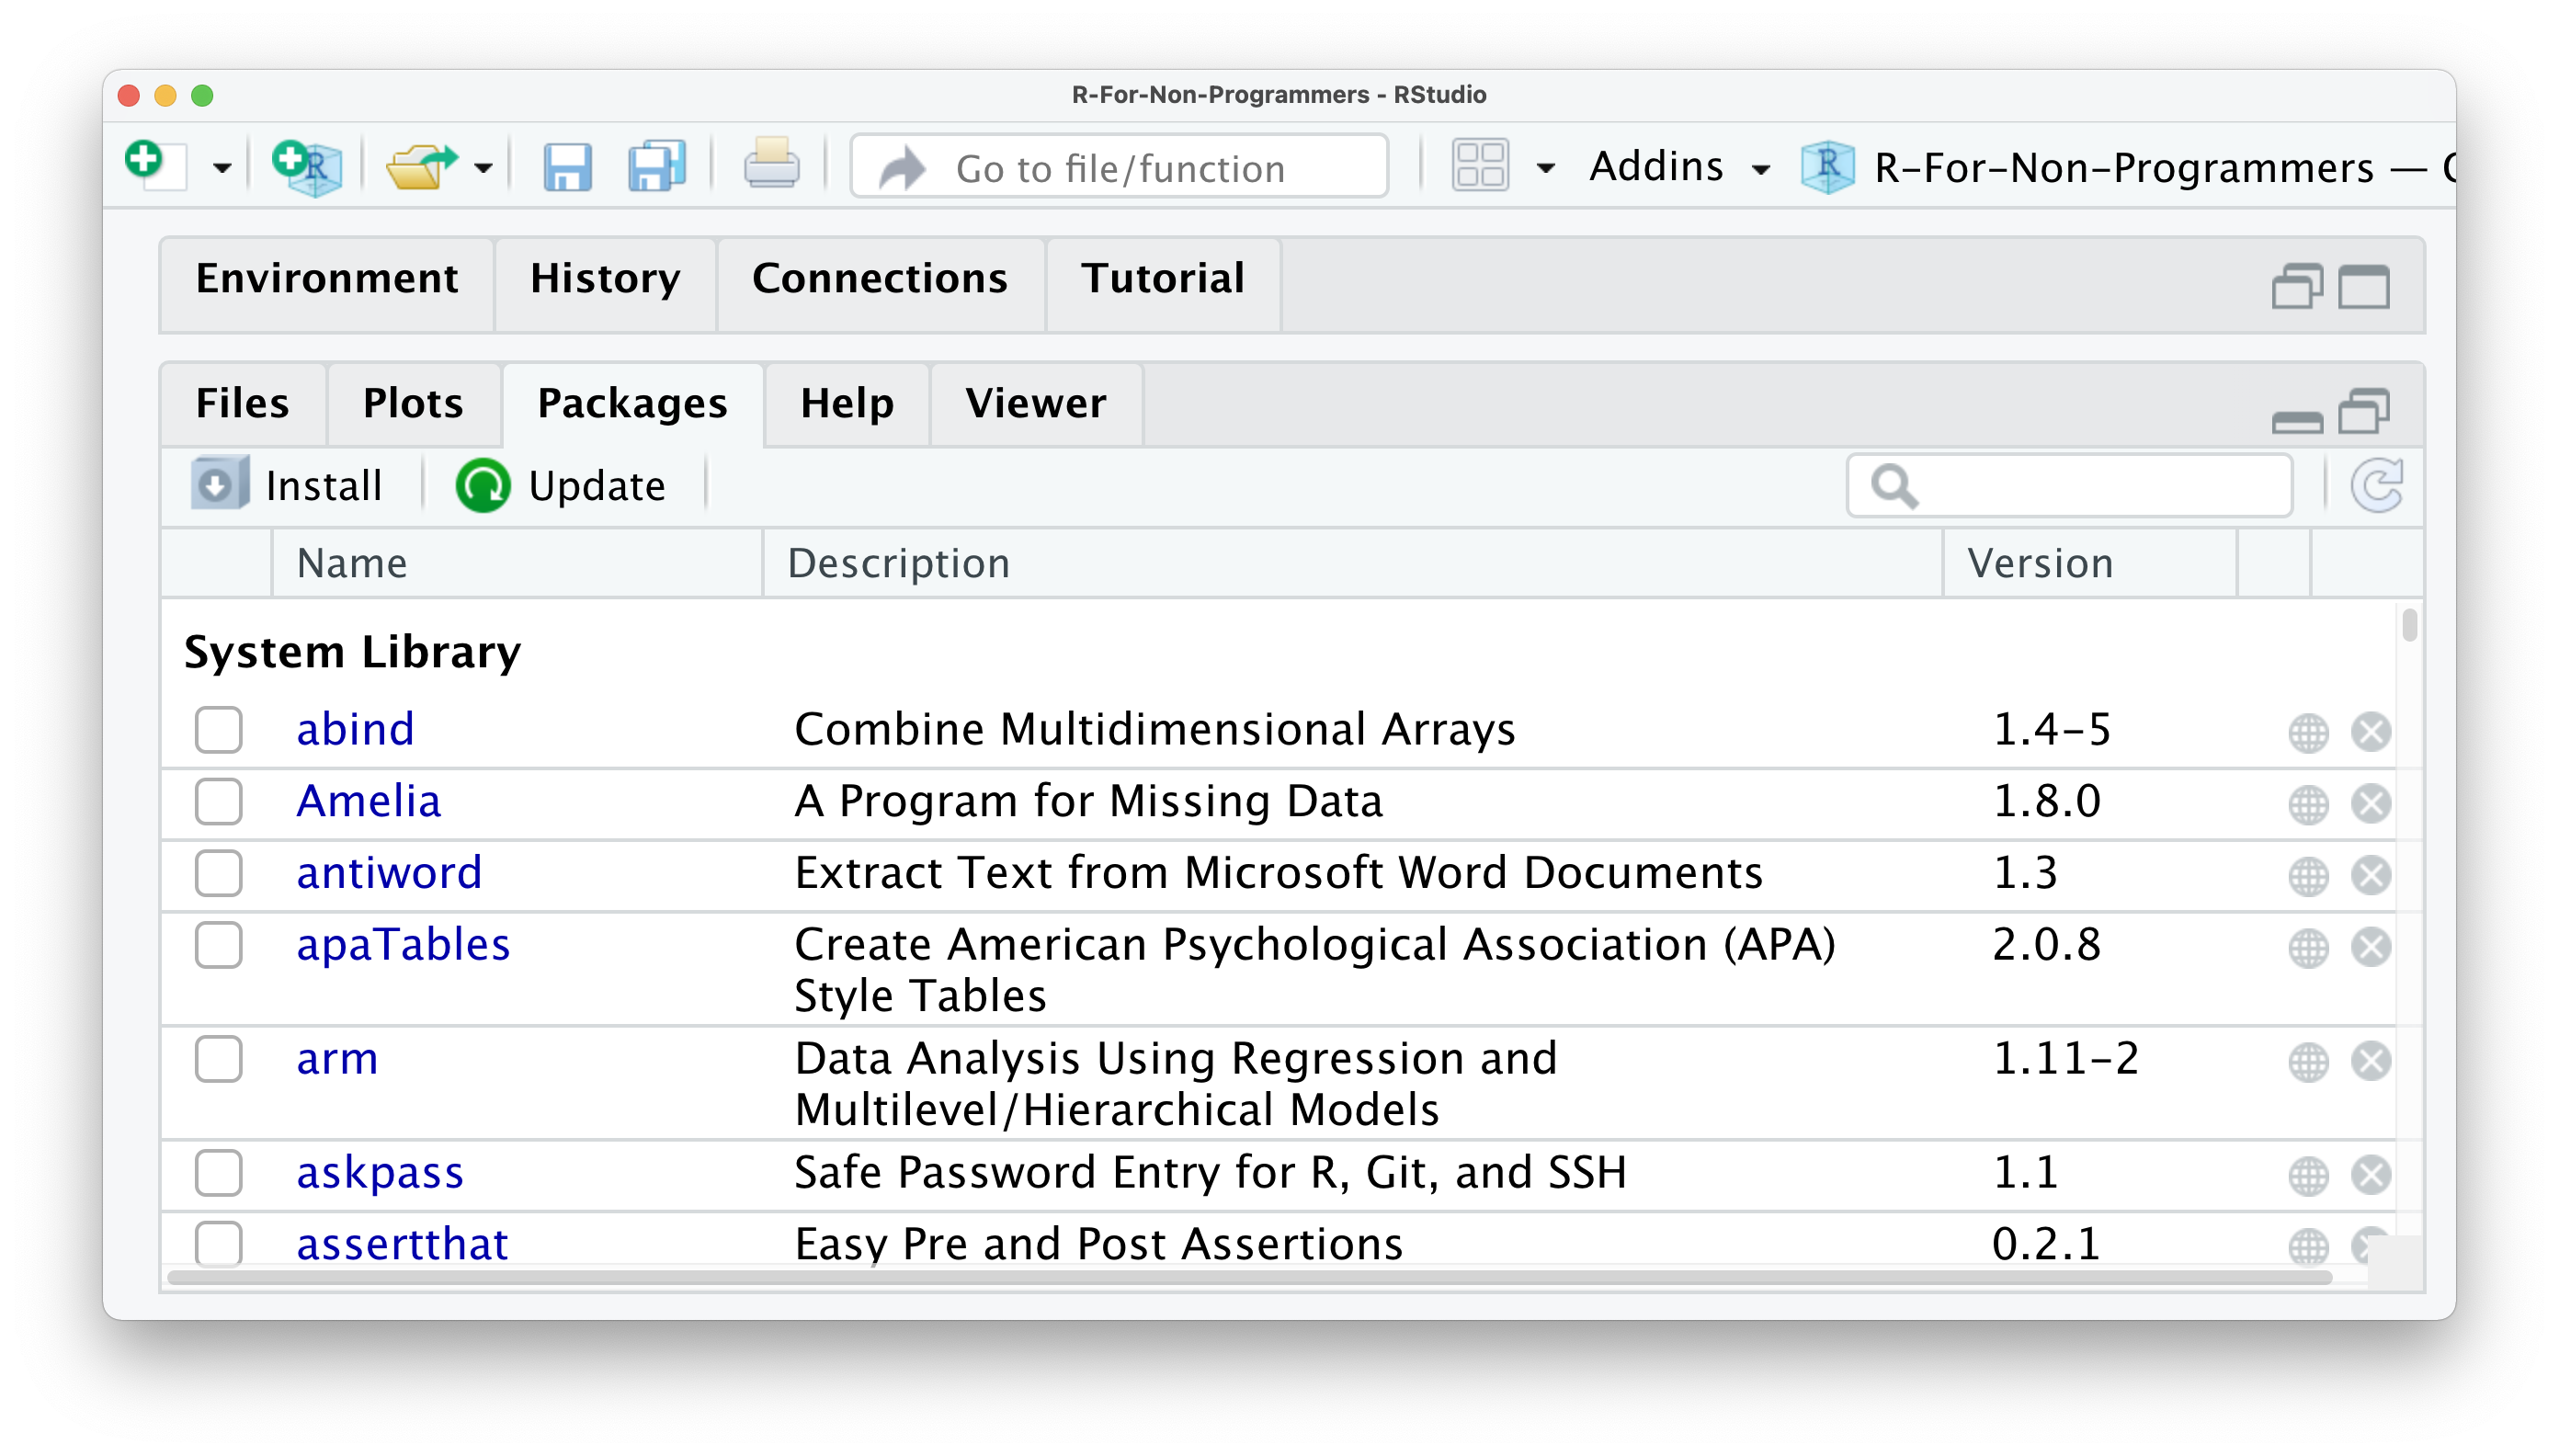
\includegraphics{images/chapter_04_img/05_files_plots_etc/03_rstudio_packages.png}

If you are in dire need of help, RStudio provides you with a \emph{Help}
pane. You can search for specific topics, for example how certain
computations work. The \emph{Help} pane also has documentation on
different datasets that are included in \emph{R}, RStudio or \emph{R
packages} you have installed. If you want a more comprehensive overview
of how you can find help, have a look at CRAN's
\href{https://www.r-project.org/help.html}{`Getting Help with R'}
webpage.

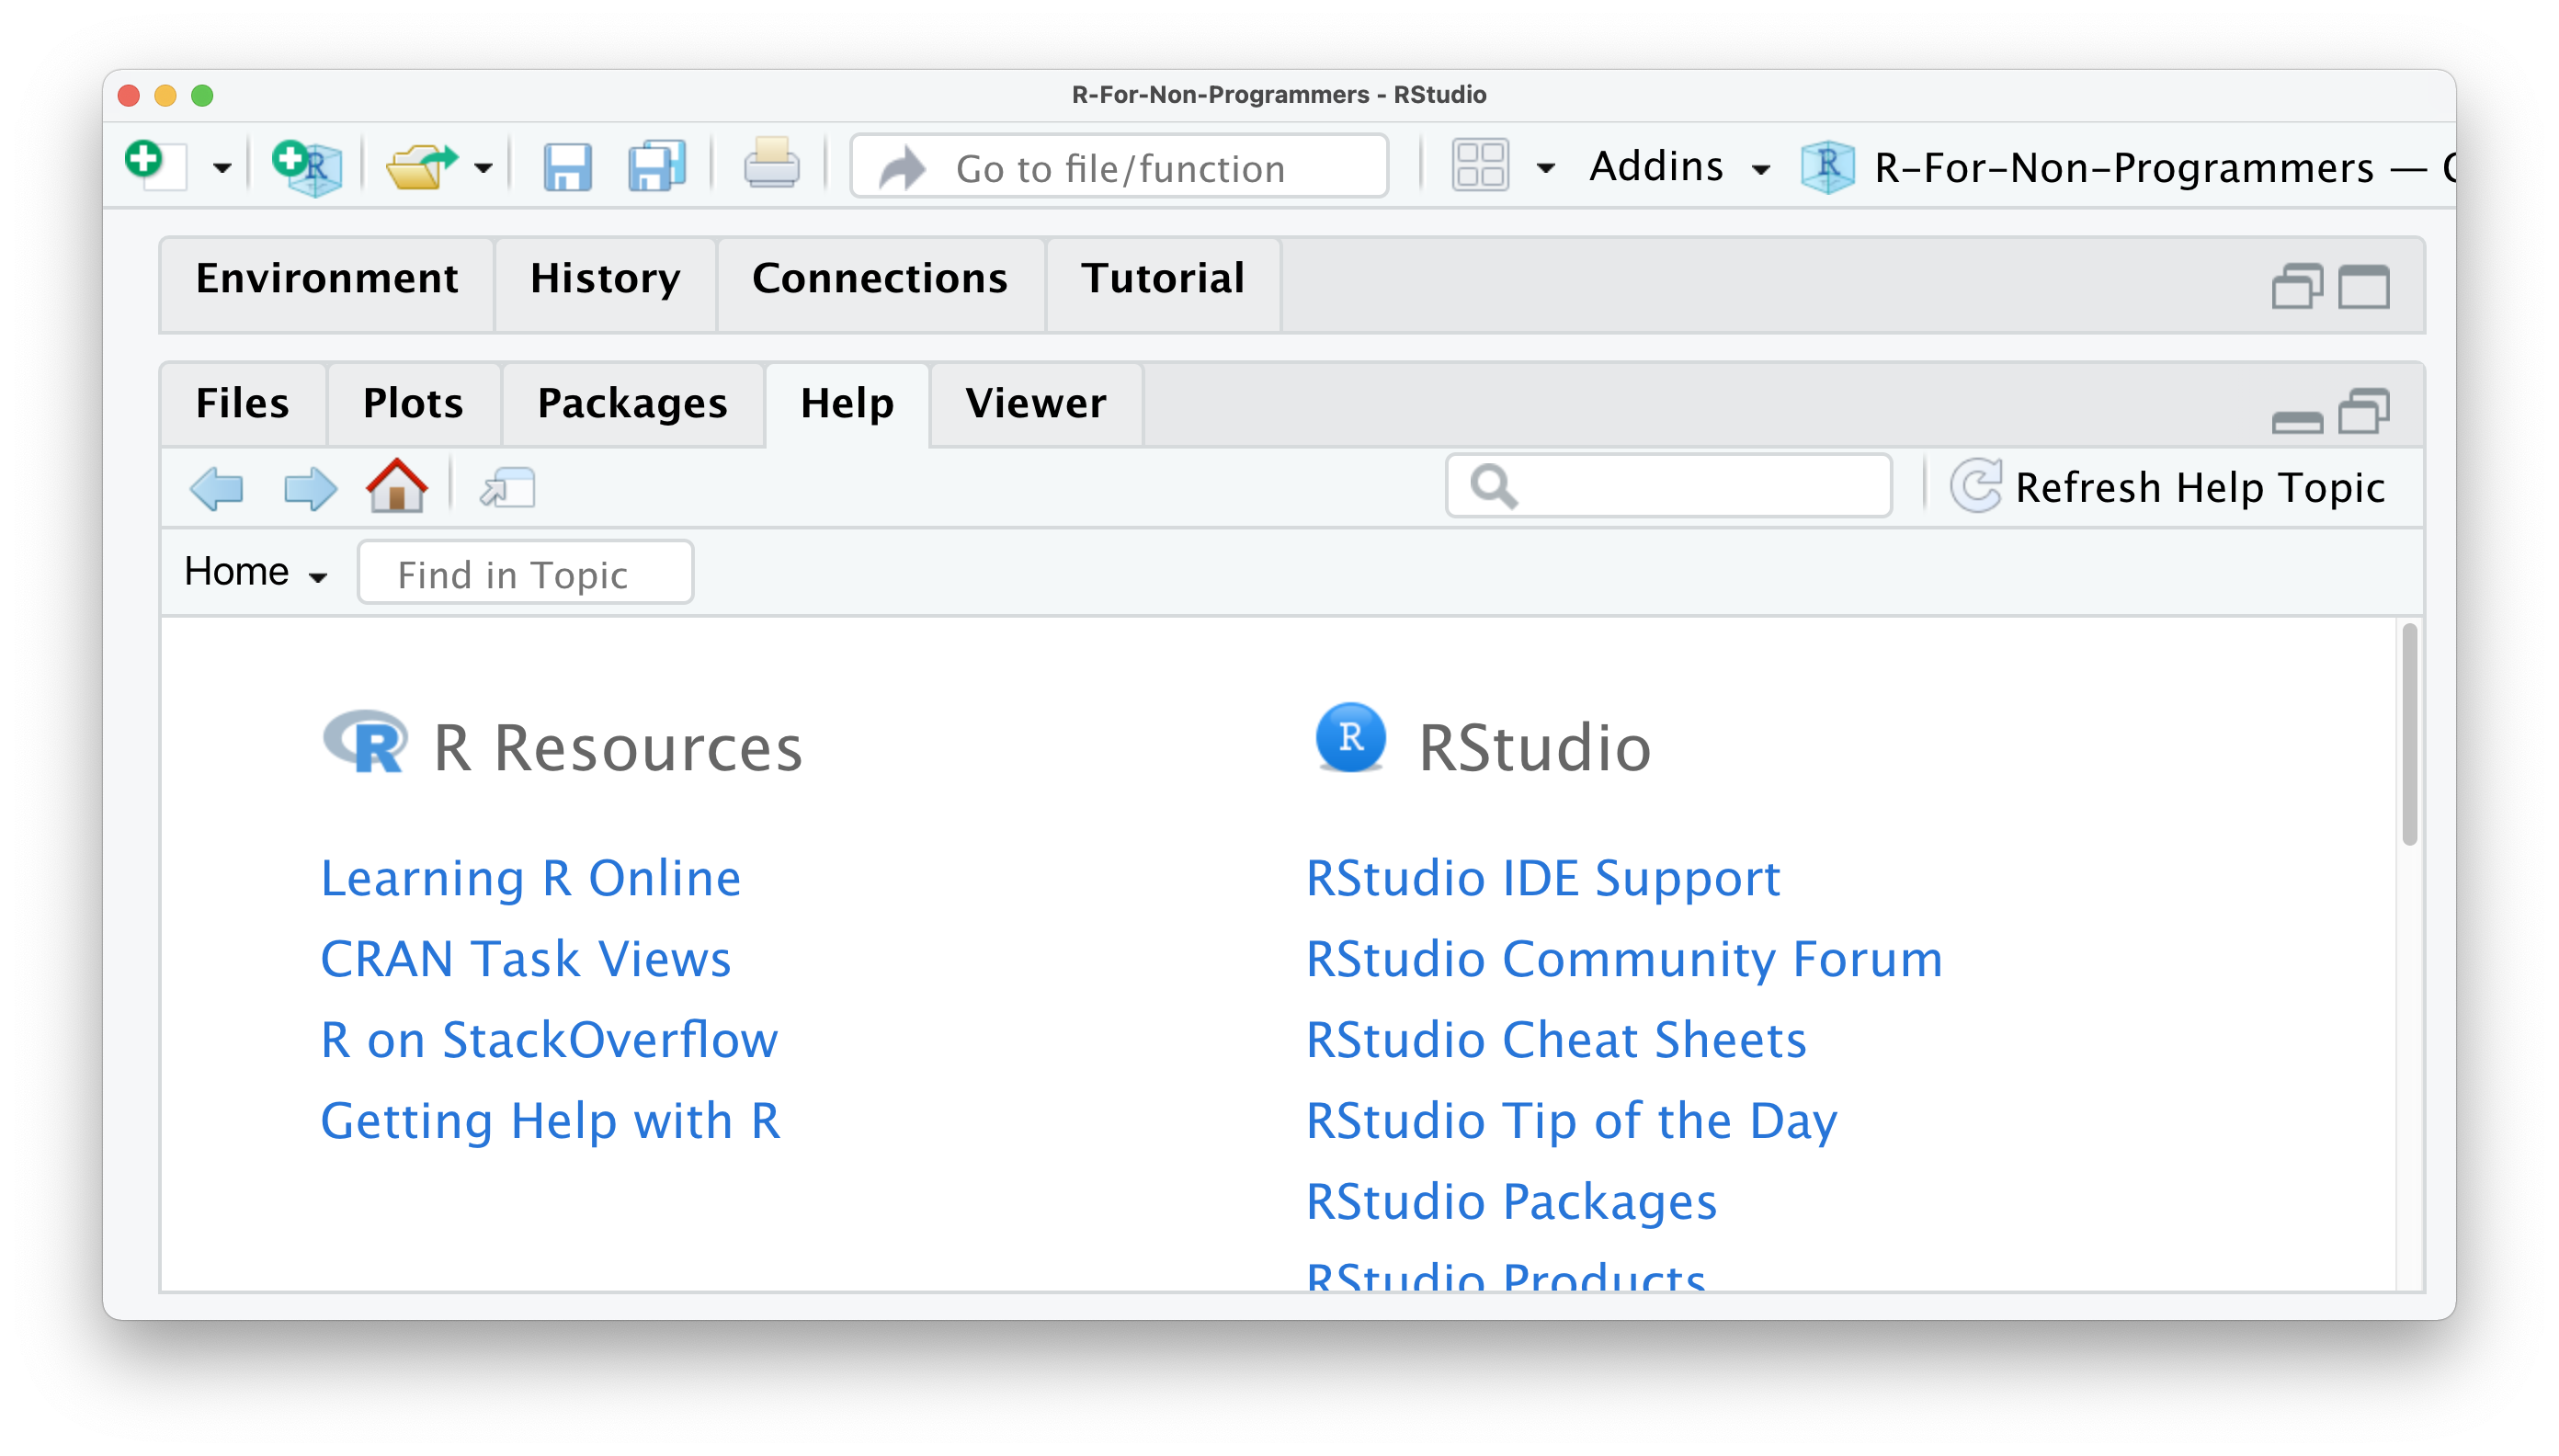
\includegraphics{images/chapter_04_img/05_files_plots_etc/04_rstudio_help.png}

So, for example, if you want to know what the \texttt{mtcars} dataset
is, you can either use the search window in the \emph{Help} pane or,
much easier, use a \texttt{?} in the console to search for it:

\begin{Shaded}
\begin{Highlighting}[]
\CommentTok{\# Type a \textquotesingle{}?\textquotesingle{} followed by the name of a dataset/function/etc.}
\CommentTok{\# to look up helpful information about it.}
\NormalTok{?mtcars}
\end{Highlighting}
\end{Shaded}

This will open the \emph{Help} pane and give you more information about
this dataset:

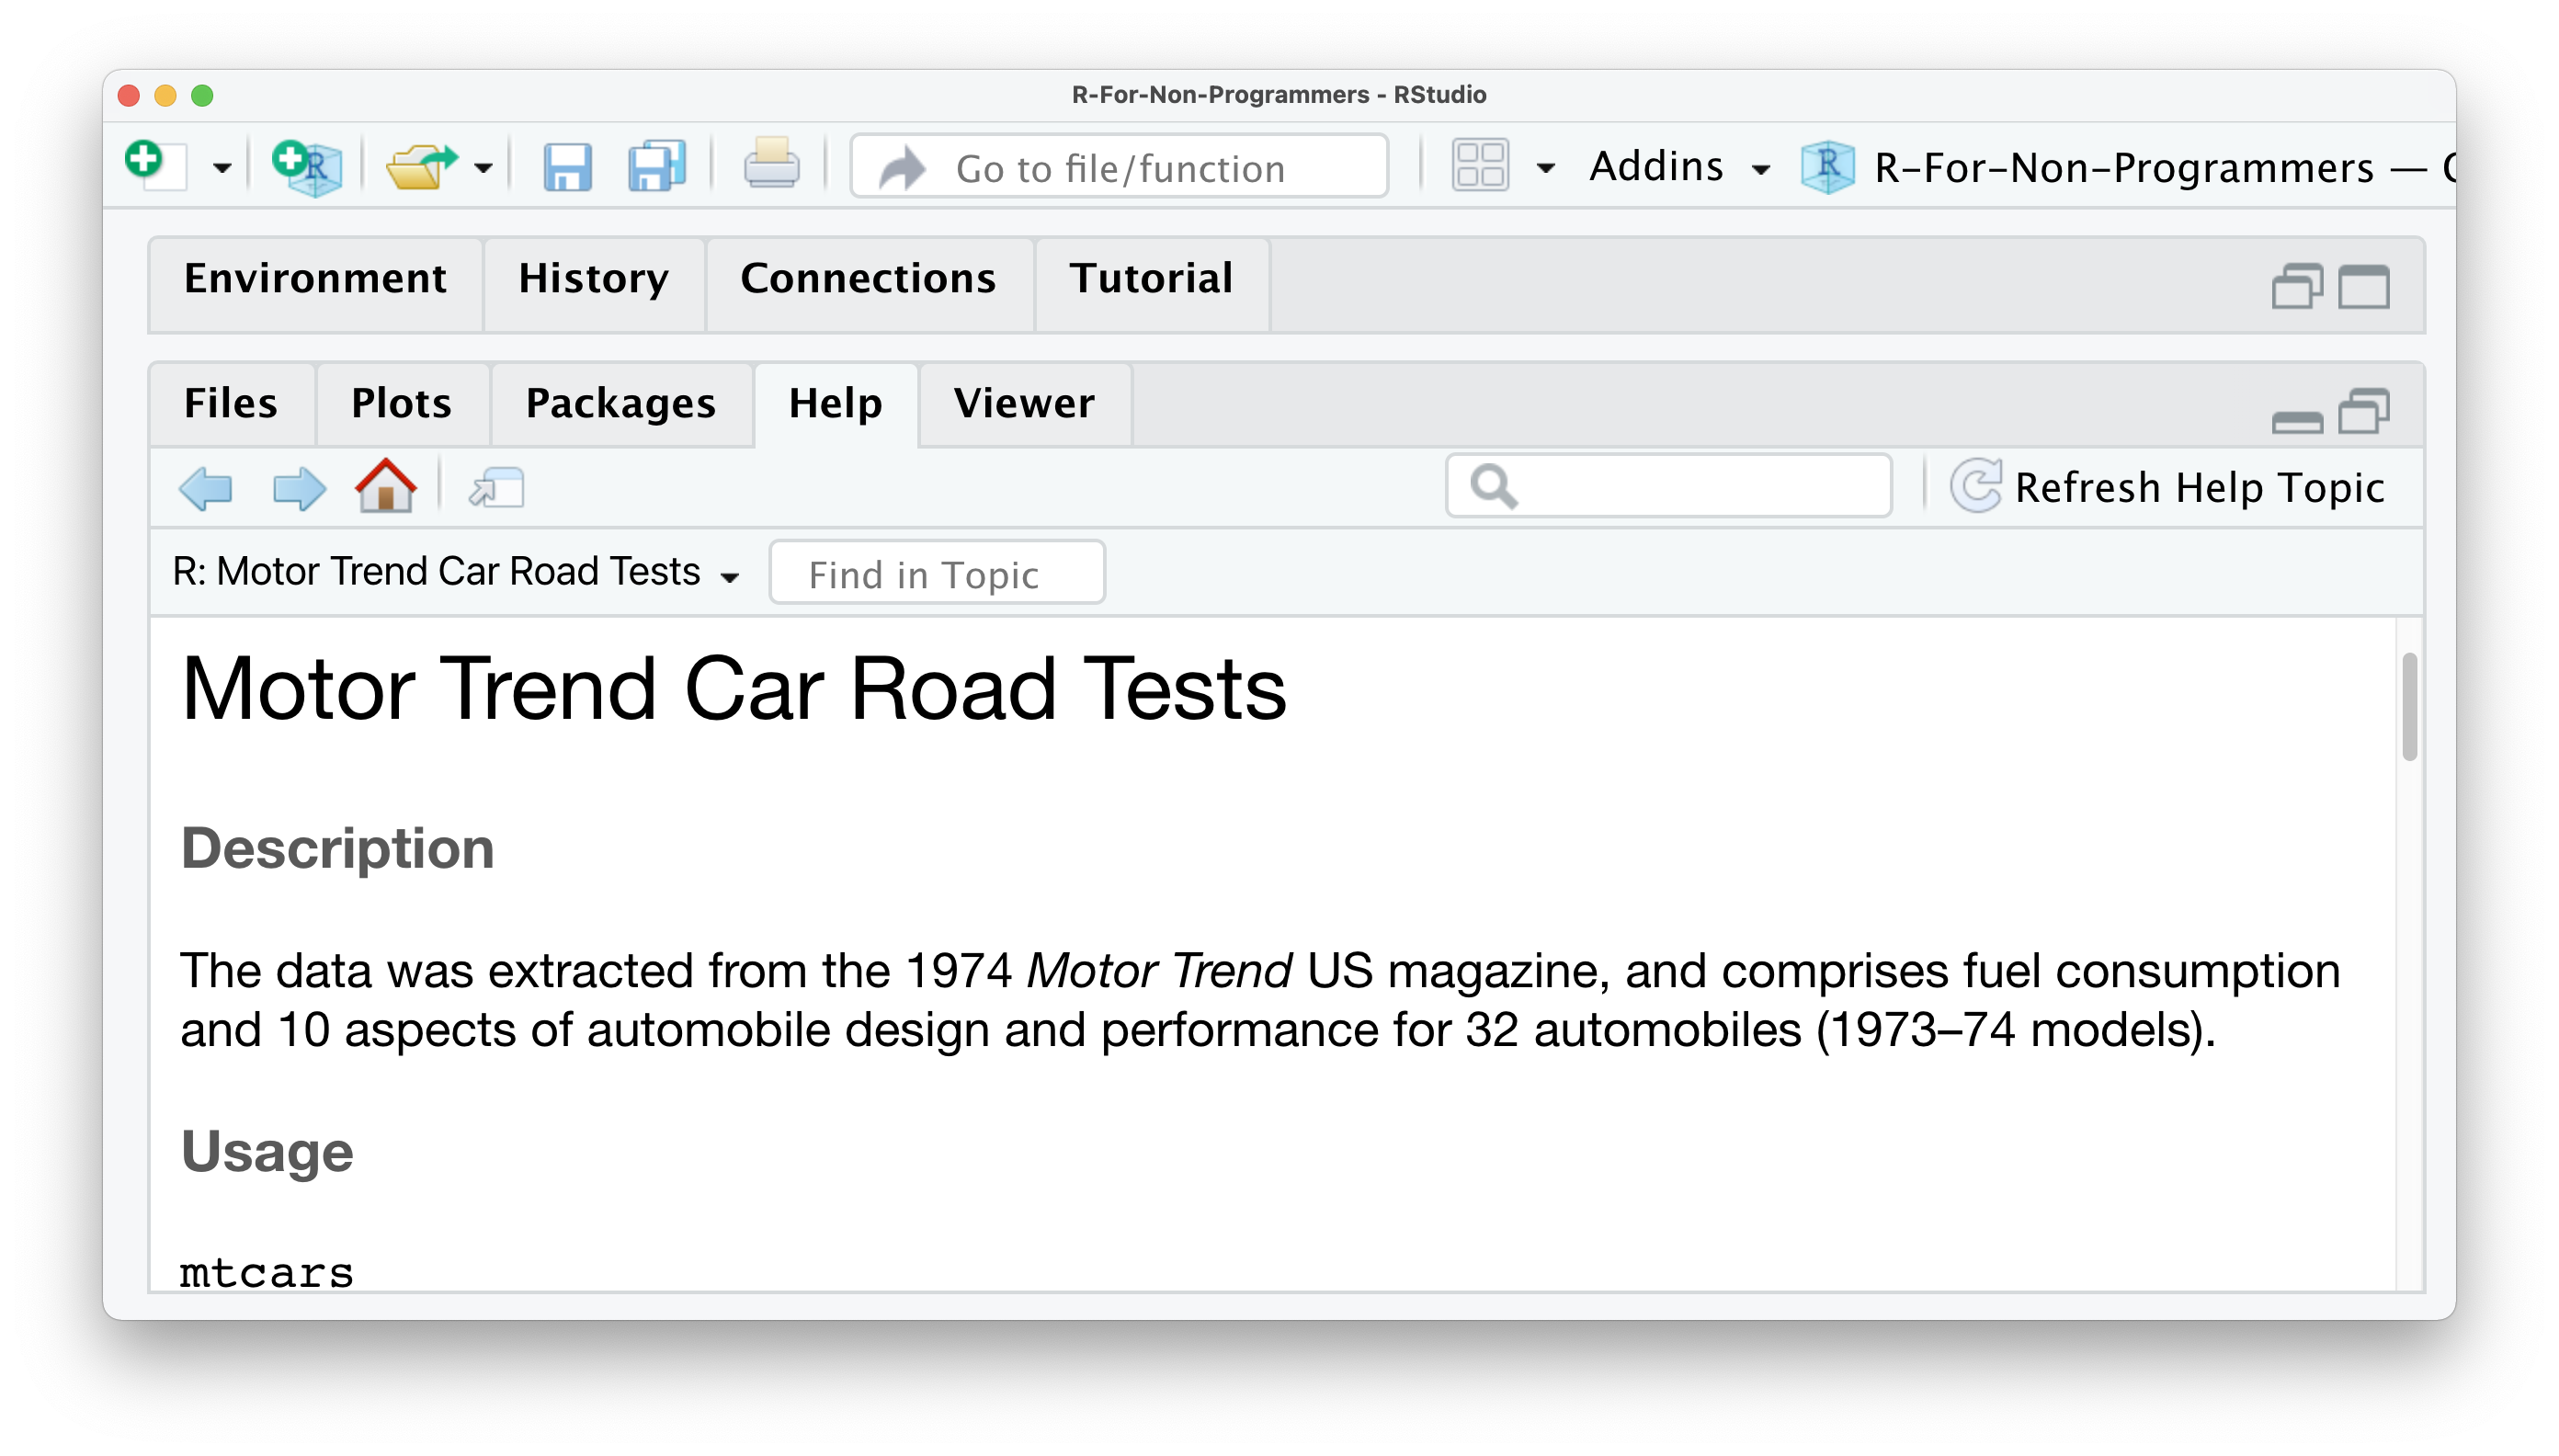
\includegraphics{images/chapter_04_img/05_files_plots_etc/04_rstudio_help_mtcars.png}

There are many different ways of how you can find help with your coding
beyond RStudio and this book. My top three platforms to find solutions
to my programming problems are:

\begin{itemize}
\item
  \href{https://www.google.com}{Google}
\item
  \href{https://stackoverflow.com}{stackoverflow.com}
\item
  \href{https://twitter.com/home}{Twitter} (with
  \href{https://twitter.com/hashtag/rstats}{\#RStats})
\end{itemize}

Lastly, we have the \emph{Viewer} pane. Not every data visualisation we
create in \emph{R} is a static image. You can create dynamic data
visualisations or even websites with \emph{R}. This type of content is
displayed in the \emph{Viewer} pane rather than in the \emph{Plots}
pane. Often these visualisations are based on HTML and other web-based
programming languages. As such, it is easy to open them in your browser
as well. However, in this book, we mainly focus on two-dimensional
static plots, which are the ones you likely need most of the time,
either for your assignments, thesis, or publication.

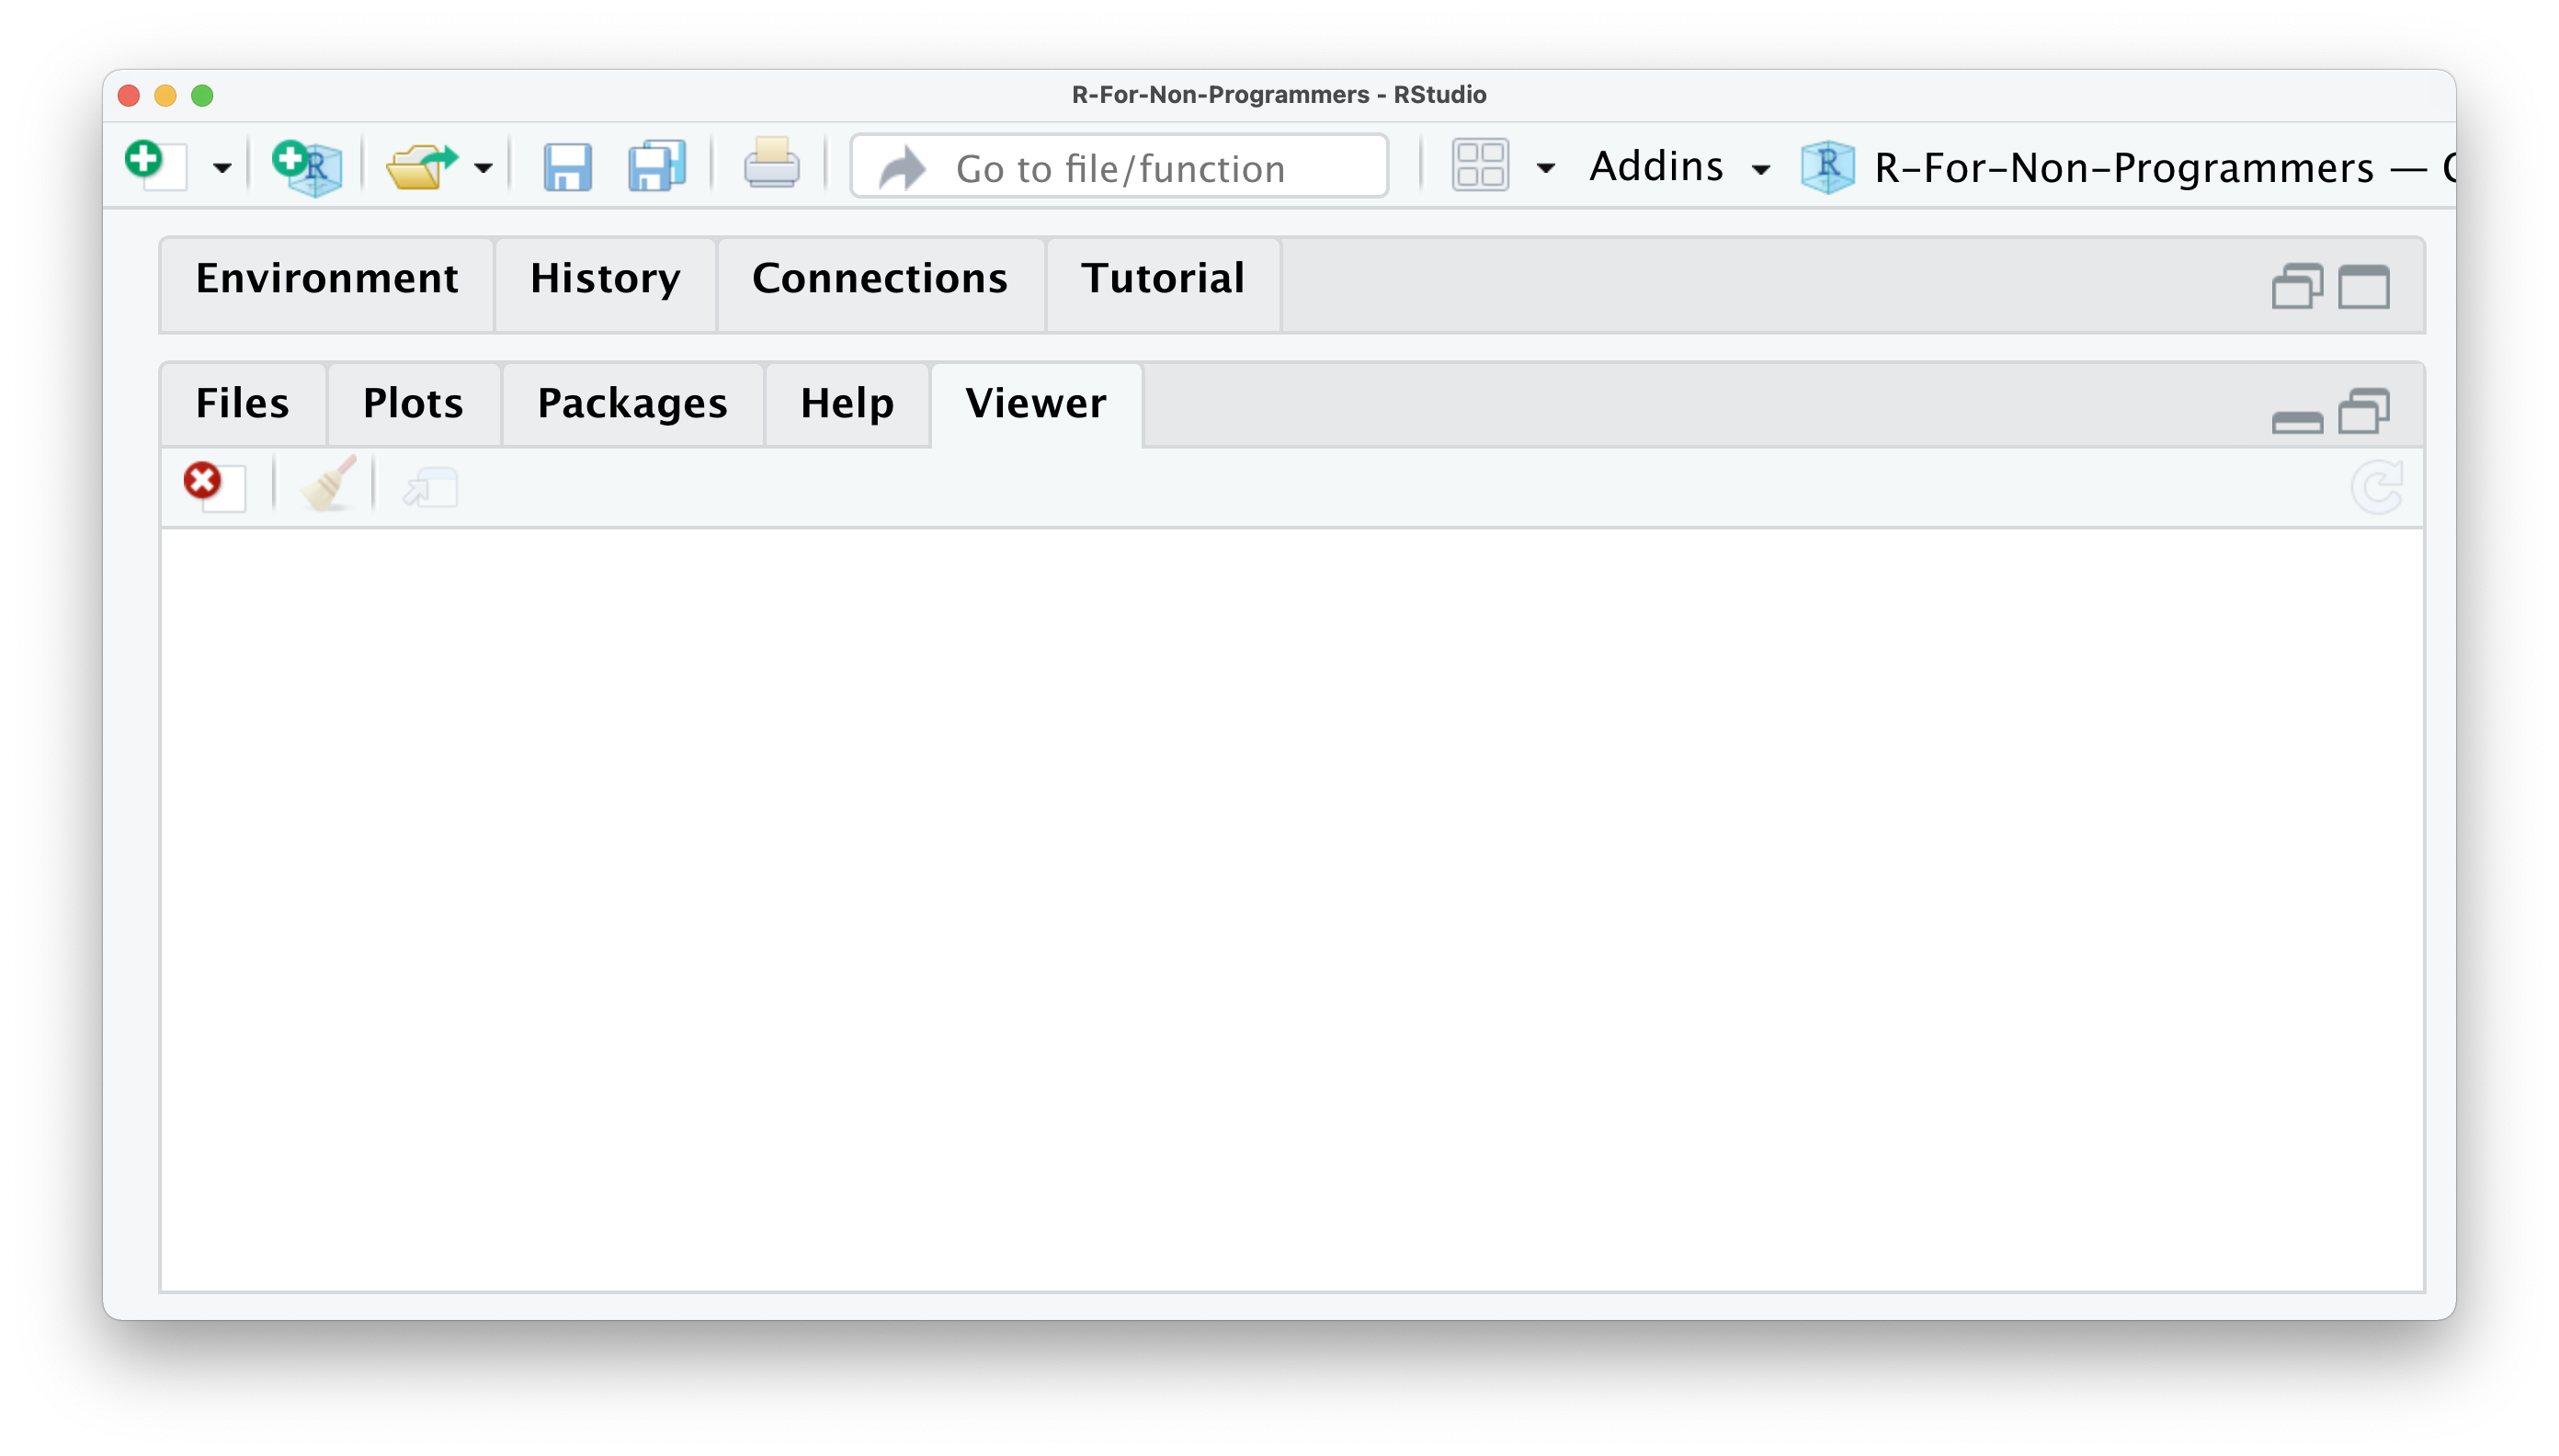
\includegraphics{images/chapter_04_img/05_files_plots_etc/05_rstudio_viewer.png}

\section{Customise your user
interface}\label{customise-your-user-interface}

As a last remark in this chapter, I would like to make you aware that
you can modify each window. There are three basic adjustments you can
make:

\begin{itemize}
\item
  Hide panes by clicking on the window symbol in the top right corner of
  each window,
\item
  Resize panes by dragging the border of a window horizontally or
  vertically, or
\item
  Add and remove panes by going to
  \texttt{RStudio\ \textgreater{}\ Preferences\ \textgreater{}\ Pane\ Layout},
  or use the keyboard shortcut \texttt{⌘\ +\ ,} if you are on a Mac.
  Unfortunately, there is no default shortcut for PC users.
\end{itemize}

If you want a fully customised experience you can also alter the colour
scheme of RStudio itself
(\texttt{RStudio\ \textgreater{}\ Preferences\ \textgreater{}\ Appearance})
and if the themes offered are not enough for you, you can create a
custom theme
\href{https://tmtheme-editor.herokuapp.com/\#!/editor/theme/Monokai}{here}.

\bookmarksetup{startatroot}

\chapter{\texorpdfstring{\emph{R} Basics: The very
fundamentals}{R Basics: The very fundamentals}}\label{r-basics-the-very-fundamentals}

After a likely tedious installation of \emph{R} and RStudio, as well as
a somewhat detailed introduction to the RStudio interface, you are
finally ready to \emph{`do'} things. By \emph{`doing'}, I mean
\emph{`coding'}. The term \emph{`coding'} in itself can instil fear in
some of you, but you only need one skill to do it: Writing. As mentioned
earlier, learning coding or programming means learning a new language.
However, once you have the basic grammar down, you already can
communicate quite a bit. In this section, we will explore the
fundamentals of \emph{R}. These build the foundation for everything that
follows. After that, we dive right into some analysis.

\section{\texorpdfstring{Basic computations in
\emph{R}}{Basic computations in R}}\label{basic-computations-in-r}

The most basic computation you can do in \emph{R} is arithmetic
operations. In other words, addition, subtraction, multiplication,
division, exponentiation and extraction of roots. In short, \emph{R} can
be used like your pocket calculator, or more likely the one you have on
your phone. For example, in Chapter @ref(the-console-window) we already
performed an addition. Thus, it might not come as a surprise how their
equivalents work in \emph{R}. Let's take a look at the following
examples:

\begin{Shaded}
\begin{Highlighting}[]
\CommentTok{\# Addition}
\DecValTok{10} \SpecialCharTok{+} \DecValTok{5}
\end{Highlighting}
\end{Shaded}

\begin{verbatim}
[1] 15
\end{verbatim}

\begin{Shaded}
\begin{Highlighting}[]
\CommentTok{\# Subtraction}
\DecValTok{10} \SpecialCharTok{{-}} \DecValTok{5}
\end{Highlighting}
\end{Shaded}

\begin{verbatim}
[1] 5
\end{verbatim}

\begin{Shaded}
\begin{Highlighting}[]
\CommentTok{\# Multiplication}
\DecValTok{10} \SpecialCharTok{*} \DecValTok{5}
\end{Highlighting}
\end{Shaded}

\begin{verbatim}
[1] 50
\end{verbatim}

\begin{Shaded}
\begin{Highlighting}[]
\CommentTok{\# Division}
\DecValTok{10} \SpecialCharTok{/} \DecValTok{5}
\end{Highlighting}
\end{Shaded}

\begin{verbatim}
[1] 2
\end{verbatim}

\begin{Shaded}
\begin{Highlighting}[]
\CommentTok{\# Exponentiation}
\DecValTok{10} \SpecialCharTok{\^{}} \DecValTok{2}
\end{Highlighting}
\end{Shaded}

\begin{verbatim}
[1] 100
\end{verbatim}

\begin{Shaded}
\begin{Highlighting}[]
\CommentTok{\# Square root}
\FunctionTok{sqrt}\NormalTok{(}\DecValTok{10}\NormalTok{)}
\end{Highlighting}
\end{Shaded}

\begin{verbatim}
[1] 3.162278
\end{verbatim}

They all look fairly straightforward except for the extraction of roots.
As you probably know, extracting the root would typically mean we use
the symbol \(\sqrt{}\) on our calculator. To compute the square root in
\emph{R}, we have to use a function instead to perform the computation.
So we first put the name of the function \texttt{sqrt} and then the
value \texttt{10} within parenthesis \texttt{()}. This results in the
following code: \texttt{sqrt(10)}. If we were to write this down in our
report, we would write \(\sqrt[2]{10}\).

Functions are an essential part of \emph{R} and programming in general.
You will learn more about them in Chapter @ref(functions). Besides
arithmetic operations, there are also logical queries you can perform.
Logical queries always return either the value \texttt{TRUE} or
\texttt{FALSE}. Here are some examples which make this clearer:

\begin{Shaded}
\begin{Highlighting}[]
\CommentTok{\#1 Is it TRUE or FALSE?}
\DecValTok{1} \SpecialCharTok{==} \DecValTok{1}
\end{Highlighting}
\end{Shaded}

\begin{verbatim}
[1] TRUE
\end{verbatim}

\begin{Shaded}
\begin{Highlighting}[]
\CommentTok{\#2 Is 45 bigger than 55?}
\DecValTok{45} \SpecialCharTok{\textgreater{}} \DecValTok{55}
\end{Highlighting}
\end{Shaded}

\begin{verbatim}
[1] FALSE
\end{verbatim}

\begin{Shaded}
\begin{Highlighting}[]
\CommentTok{\#3 Is 1982 bigger or equal to 1982?}
\DecValTok{1982} \SpecialCharTok{\textgreater{}=} \DecValTok{1982}
\end{Highlighting}
\end{Shaded}

\begin{verbatim}
[1] TRUE
\end{verbatim}

\begin{Shaded}
\begin{Highlighting}[]
\CommentTok{\#4 Are these two words NOT the same?}
\StringTok{"Friends"} \SpecialCharTok{!=} \StringTok{"friends"}
\end{Highlighting}
\end{Shaded}

\begin{verbatim}
[1] TRUE
\end{verbatim}

\begin{Shaded}
\begin{Highlighting}[]
\CommentTok{\#5 Are these sentences the same?}
\StringTok{"I love statistics"} \SpecialCharTok{==} \StringTok{"I love statistícs"}
\end{Highlighting}
\end{Shaded}

\begin{verbatim}
[1] FALSE
\end{verbatim}

Reflecting on these examples, you might notice three important aspects
of logical queries:

\begin{enumerate}
\def\labelenumi{\arabic{enumi}.}
\tightlist
\item
  We have to use \texttt{==} instead of \texttt{=},
\item
  We can compare non-numerical values, i.e.~text, which is also known as
  \texttt{character} values, with each other,
\item
  The devil is in the details (consider \#5).
\end{enumerate}

One of the most common mistakes of \emph{R} novices is the confusion
around the \texttt{==} and \texttt{=} notation. While \texttt{==}
represents \texttt{equal\ to}, \texttt{=} is used to assign a value to
an object (for more details on assignments see Chapter
@ref(assigning-values-to-objects)). However, in practice, most \emph{R}
programmers tend to avoid \texttt{=} since it can easily lead to
confusion with \texttt{==}. As such, you can strike \texttt{=} out of
your R vocabulary for now.

There are many different logical operations you can perform. Table
@ref(tab:logical-operators-r) lists the most frequently used logical
operators for your reference. These will become important, for example
when we filter our data for analysis, e.g.~include only female or male
participants.

\begin{longtable}{cl}
\caption{Logical operators in R}\tabularnewline

\toprule
Operator & Description \\ 
\midrule\addlinespace[2.5pt]
== & is equal to \\ 
!= & is not equal to \\ 
>= & is bigger or equal to \\ 
> & is bigger than \\ 
<= & is smaller or equal to \\ 
< & is smaller than \\ 
a | b & a or b \\ 
a \& b & a and b \\ 
!a & is not a \\ 
\bottomrule
\end{longtable}

\section{Assigning values to objects:
`\textless-'}\label{assigning-values-to-objects}

Another common task you will perform is assigning values to an object.
An object can be many different things:

\begin{itemize}
\item
  a dataset,
\item
  the results of a computation,
\item
  a plot,
\item
  a series of numbers,
\item
  a list of names,
\item
  a function,
\item
  etc.
\end{itemize}

In short, an object is an umbrella term for many different things which
form part of your data analysis. For example, objects are handy when
storing results that you want to process further in later analytical
steps. We have to use the assign operator \texttt{\textless{}-} to
assign a value to an object. Let's have a look at an example.

\begin{Shaded}
\begin{Highlighting}[]
\CommentTok{\# I have a friend called "Fiona"}
\NormalTok{friends }\OtherTok{\textless{}{-}} \StringTok{"Fiona"}
\end{Highlighting}
\end{Shaded}

In this example, I created an object called \texttt{friends} and added
\texttt{"Fiona"} to it. Since \texttt{"Fiona"} represents a
\texttt{string}, we need to use \texttt{""}. So, if you wanted to read
this line of code, you would say, `\texttt{friends} gets the value
\texttt{"Fiona"}'. Alternatively, you could also say `\texttt{"Fiona"}
is assigned to \texttt{friends}'.

If you look into your environment pane, you will find the object
\texttt{friends}. You can see it carries the value \texttt{"Fiona"}. We
can also print values of an object in the console by simply typing the
name of the object \texttt{friends} and hit \texttt{Return\ ↵}.

\begin{Shaded}
\begin{Highlighting}[]
\CommentTok{\# Who are my friends?}
\NormalTok{friends}
\end{Highlighting}
\end{Shaded}

\begin{verbatim}
[1] "Fiona"
\end{verbatim}

Sadly, it seems I only have one friend. Luckily we can add some more,
not the least to make me feel less lonely. To create objects with
multiple values, we can use the function \texttt{c()}, which stands for
`concatenate'. The Cambridge Dictionary (2021) defines this word as
follows:

\begin{quote}
`\textbf{\emph{concatenate}}',

\emph{to put things together as a connected series.}
\end{quote}

Let's concatenate some more friends into our \texttt{friends} object.

\begin{Shaded}
\begin{Highlighting}[]
\CommentTok{\# Adding some more friends to my life}
\NormalTok{friends }\OtherTok{\textless{}{-}} \FunctionTok{c}\NormalTok{(}\StringTok{"Fiona"}\NormalTok{,}
             \StringTok{"Lukas"}\NormalTok{,}
             \StringTok{"Ida"}\NormalTok{,}
             \StringTok{"Georg"}\NormalTok{,}
             \StringTok{"Daniel"}\NormalTok{,}
             \StringTok{"Pavel"}\NormalTok{,}
             \StringTok{"Tigger"}\NormalTok{)}

\CommentTok{\# Here are all my friends}
\NormalTok{friends}
\end{Highlighting}
\end{Shaded}

\begin{verbatim}
[1] "Fiona"  "Lukas"  "Ida"    "Georg"  "Daniel" "Pavel"  "Tigger"
\end{verbatim}

To concatenate values into a single object, we need to use a comma
\texttt{,} to separate each value. Otherwise, \emph{R} will report an
error back.

\begin{Shaded}
\begin{Highlighting}[]
\NormalTok{friends }\OtherTok{\textless{}{-}} \FunctionTok{c}\NormalTok{(}\StringTok{"Fiona"} \StringTok{"Ida"}\NormalTok{)}
\end{Highlighting}
\end{Shaded}

\emph{R}'s error messages tend to be very useful and give meaningful
clues to what went wrong. In this case, we can see that something
`\emph{unexpected}' happened, and it shows where our mistake is. You can
also concatenate numbers

Btw, if you add \texttt{()} around your code, you can automatically
print the content of the object to the console. Thus,

\begin{itemize}
\item
  \texttt{(milestones\_of\_my\_life\ \textless{}-\ c(1982,\ 2006,\ 2011,\ 2018,\ 2020))}
  is the same as
\item
  \texttt{milestones\_of\_my\_life\ \textless{}-\ c(1982,\ 2006,\ 2011,\ 2018,\ 2020)}
  followed by \texttt{milestones\_of\_my\_life}.
\end{itemize}

You can copy and paste the following example to illustrate what I
explained.

\begin{Shaded}
\begin{Highlighting}[]
\CommentTok{\# Important years in my life}
\NormalTok{milestones\_of\_my\_life }\OtherTok{\textless{}{-}} \FunctionTok{c}\NormalTok{(}\DecValTok{1982}\NormalTok{, }\DecValTok{2006}\NormalTok{, }\DecValTok{2011}\NormalTok{, }\DecValTok{2018}\NormalTok{, }\DecValTok{2020}\NormalTok{)}
\NormalTok{milestones\_of\_my\_life}
\end{Highlighting}
\end{Shaded}

\begin{verbatim}
[1] 1982 2006 2011 2018 2020
\end{verbatim}

\begin{Shaded}
\begin{Highlighting}[]
\CommentTok{\# The same as above {-} no second line of code needed}
\NormalTok{(milestones\_of\_my\_life }\OtherTok{\textless{}{-}} \FunctionTok{c}\NormalTok{(}\DecValTok{1982}\NormalTok{, }\DecValTok{2006}\NormalTok{, }\DecValTok{2011}\NormalTok{, }\DecValTok{2018}\NormalTok{, }\DecValTok{2020}\NormalTok{))}
\end{Highlighting}
\end{Shaded}

\begin{verbatim}
[1] 1982 2006 2011 2018 2020
\end{verbatim}

Finally, we can also concatenate numbers and character values into one
object:

\begin{Shaded}
\begin{Highlighting}[]
\NormalTok{(names\_and\_years }\OtherTok{\textless{}{-}} \FunctionTok{c}\NormalTok{(}\StringTok{"Fiona"}\NormalTok{, }\DecValTok{1988}\NormalTok{, }\StringTok{"Daniel"}\NormalTok{, }\DecValTok{1982}\NormalTok{))}
\end{Highlighting}
\end{Shaded}

\begin{verbatim}
[1] "Fiona"  "1988"   "Daniel" "1982"  
\end{verbatim}

This last example is not necessarily something I would recommend to do,
because it likely leads to undesirable outcomes. For example, if you
look into your environment pane you currently have three objects:
\texttt{friends}, \texttt{milestones\_of\_my\_life}, and
\texttt{names\_and\_years}.

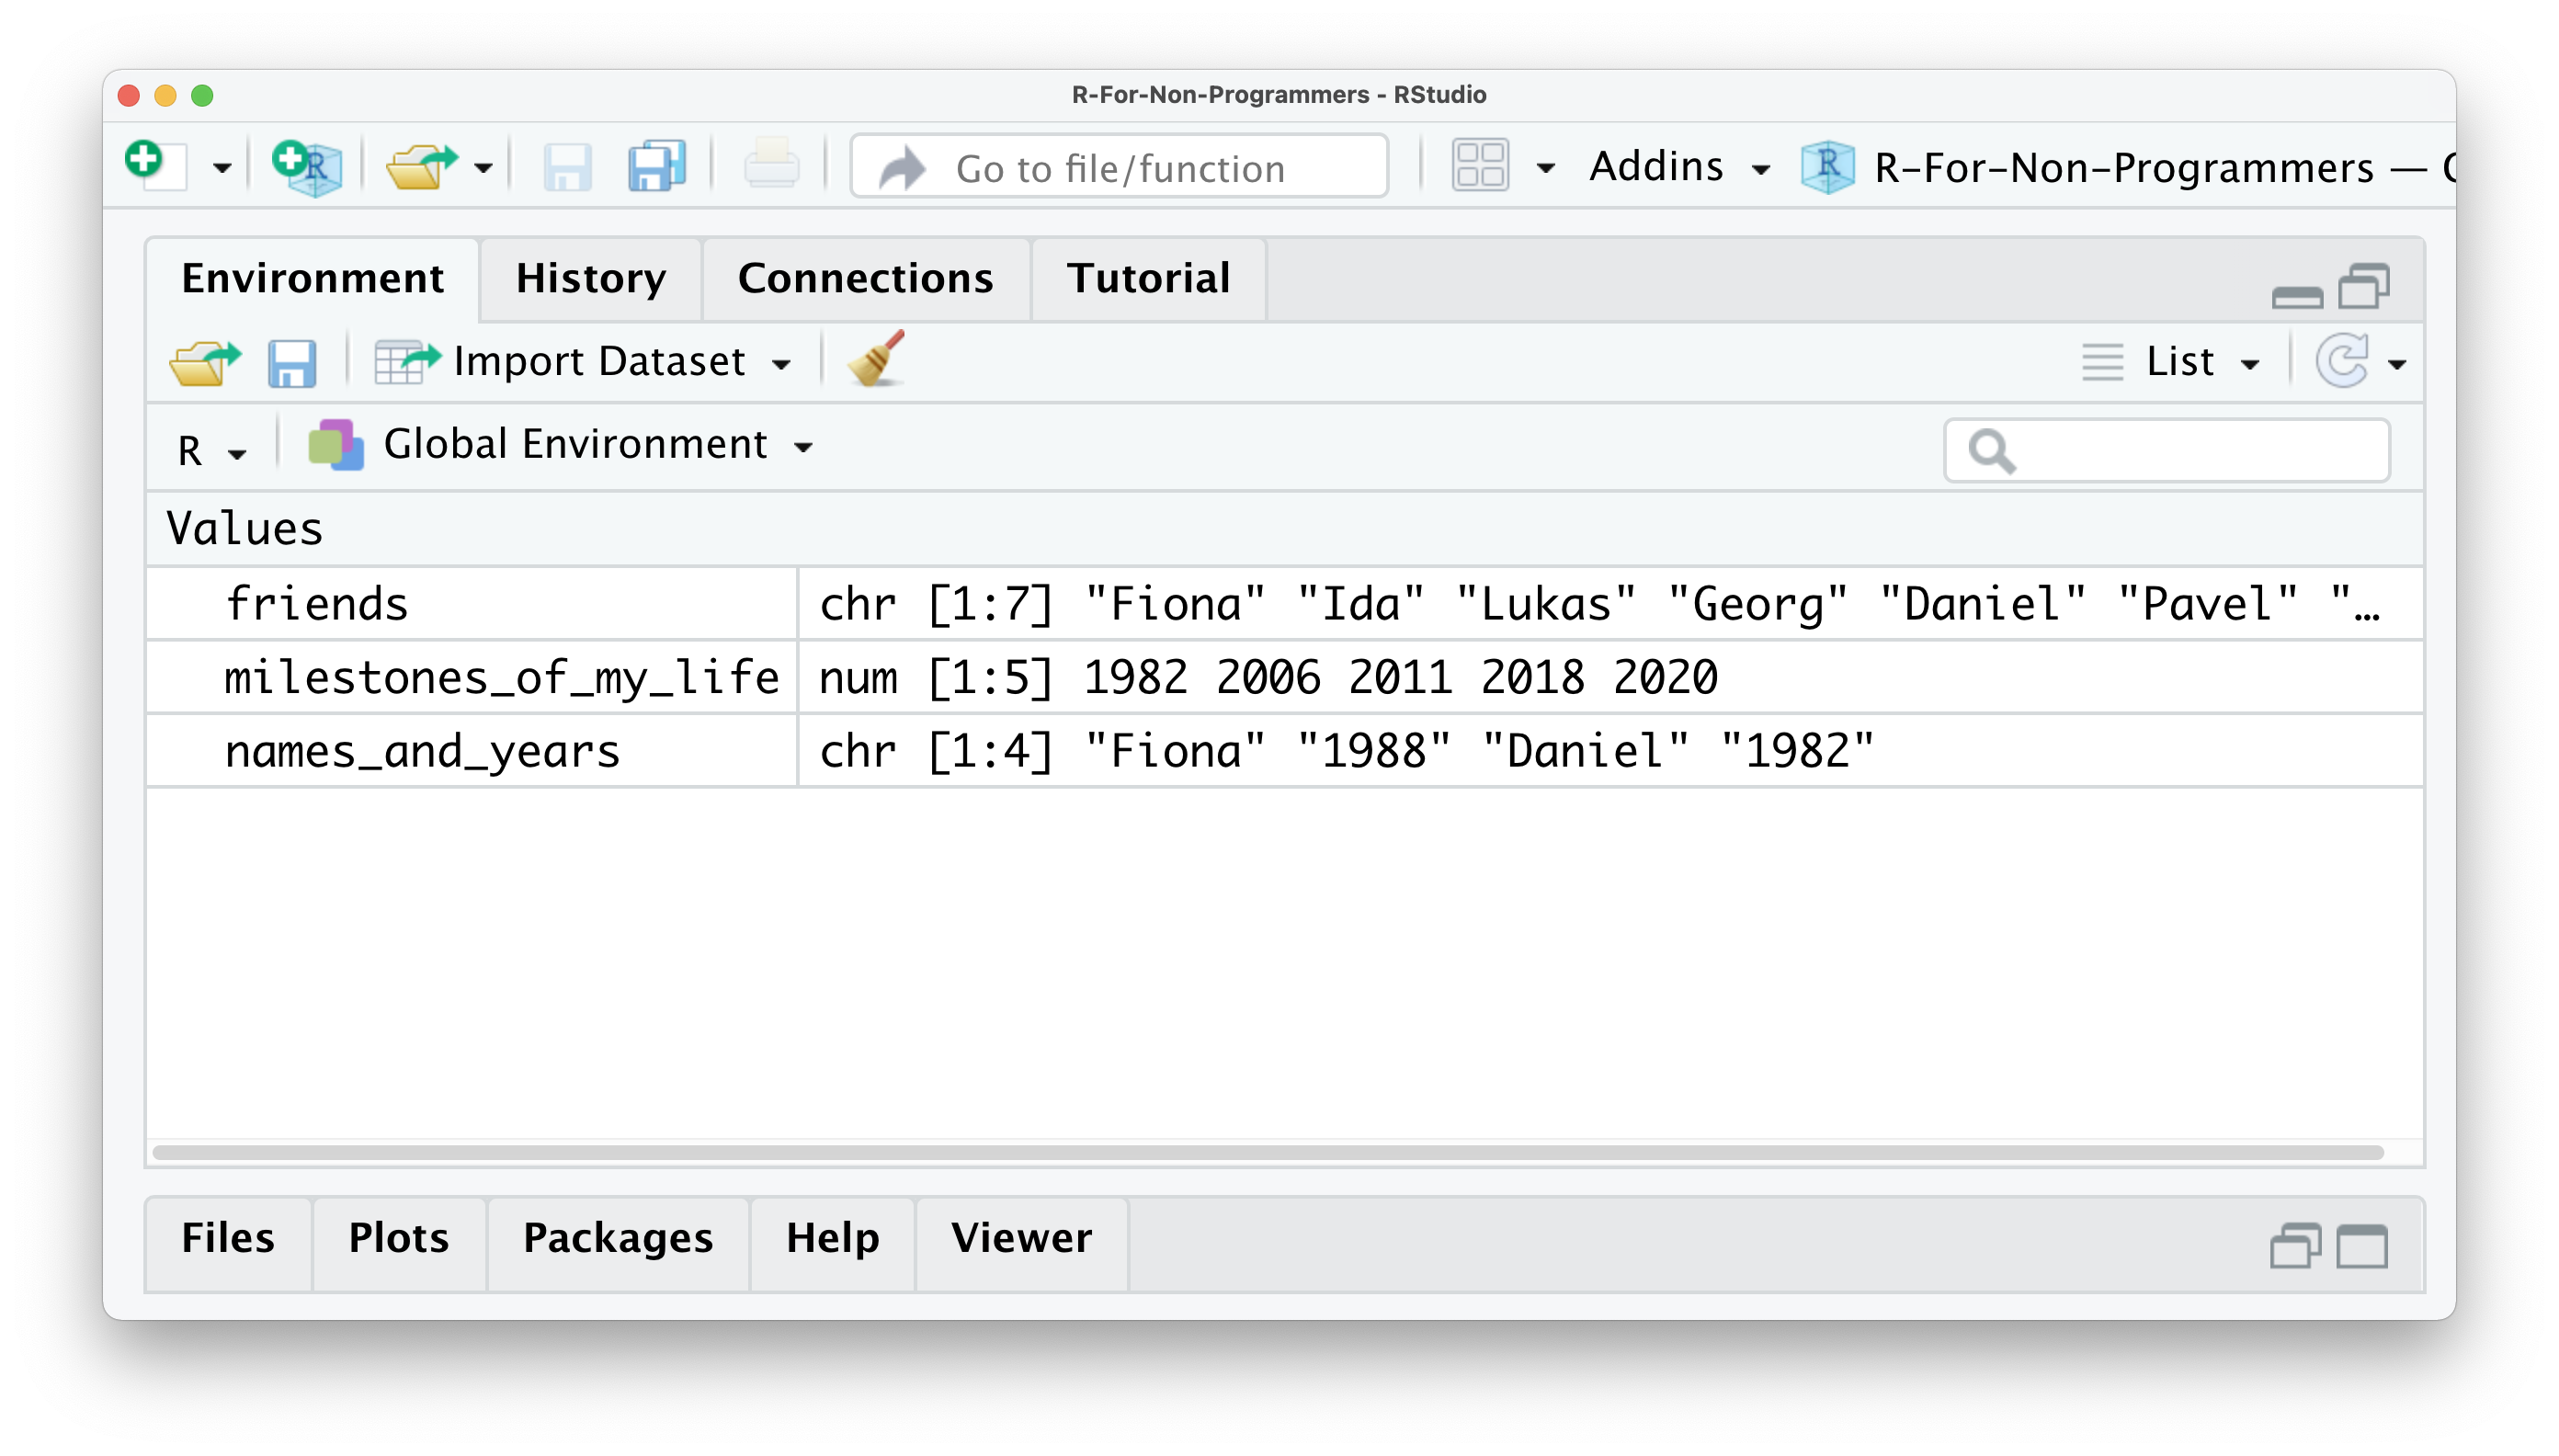
\includegraphics{images/chapter_05_img/01_basic_computation_environment_objects.png}

The \texttt{friends} object shows that all the values inside the object
are classified as \texttt{chr}, which denominates \texttt{character}.
For this object, this is correct because it only includes the names of
my friends. On the other hand, the object
\texttt{milestones\_of\_my\_life} only includes \texttt{numeric} values,
and therefore it says \texttt{num} in the environment pane. However, for
the object \texttt{names\_and\_years} we know we want to have
\texttt{numeric} and \texttt{character} values included. Still, \emph{R}
recognises them as \texttt{character} values because values inside
objects are meant to be of the same type. Remember that in \emph{R,}
numbers can always be interpreted as \texttt{character} and
\texttt{numeric}, but text only can be considered as \texttt{character}.

Consequently, mixing different types of data into one object is likely a
bad idea. This is especially true if you want to use the
\texttt{numeric} values for computation. We will return to data types in
Chapter @ref(change-data-types) where we learn how to change them, but
for now we should ensure that our objects are all of the same data type.

However, there is an exception to this rule. `Of course', you might say.
There is one object that can have values of different types: a
\texttt{list}. As the name indicates, a \texttt{list} object holds
several items. These items are usually other objects. In the spirit of
`\href{https://www.imdb.com/title/tt1375666/?ref_=ext_shr_lnk}{Inception}',
you can have lists inside lists, which contain more lists or other
objects.

Let's create a \texttt{list} called \texttt{x\_files} using the
\texttt{list} function and place all our objects inside.

\begin{Shaded}
\begin{Highlighting}[]
\CommentTok{\# This creates our list of objects}
\NormalTok{x\_files }\OtherTok{\textless{}{-}} \FunctionTok{list}\NormalTok{(friends,}
\NormalTok{                milestones\_of\_my\_life,}
\NormalTok{                names\_and\_years)}

\CommentTok{\# Let\textquotesingle{}s have a look what is hidden inside the x\_files}
\NormalTok{x\_files}
\end{Highlighting}
\end{Shaded}

\begin{verbatim}
[[1]]
[1] "Fiona"  "Lukas"  "Ida"    "Georg"  "Daniel" "Pavel"  "Tigger"

[[2]]
[1] 1982 2006 2011 2018 2020

[[3]]
[1] "Fiona"  "1988"   "Daniel" "1982"  
\end{verbatim}

You will notice in this example that I do not use \texttt{""} for each
value in the list. This is because \texttt{friends} is not a
\texttt{character} value, but an object. When we refer to objects, we do
not need quotation marks.

We will encounter \texttt{list} objects quite frequently when we perform
our analysis. Some functions return the results in the format of lists.
This can be very helpful because otherwise our environment pane will be
littered with objects and we would not necessarily know how they relate
to each other, or worse, to which analysis they belong. Looking at the
list item in the environment page (Figure~\ref{fig-img-x-files}), you
can see that the object \texttt{x\_files} is classified as a
\texttt{List\ of\ 3,} and if you click on the blue icon, you can inspect
the different objects inside.

\begin{figure}

\centering{

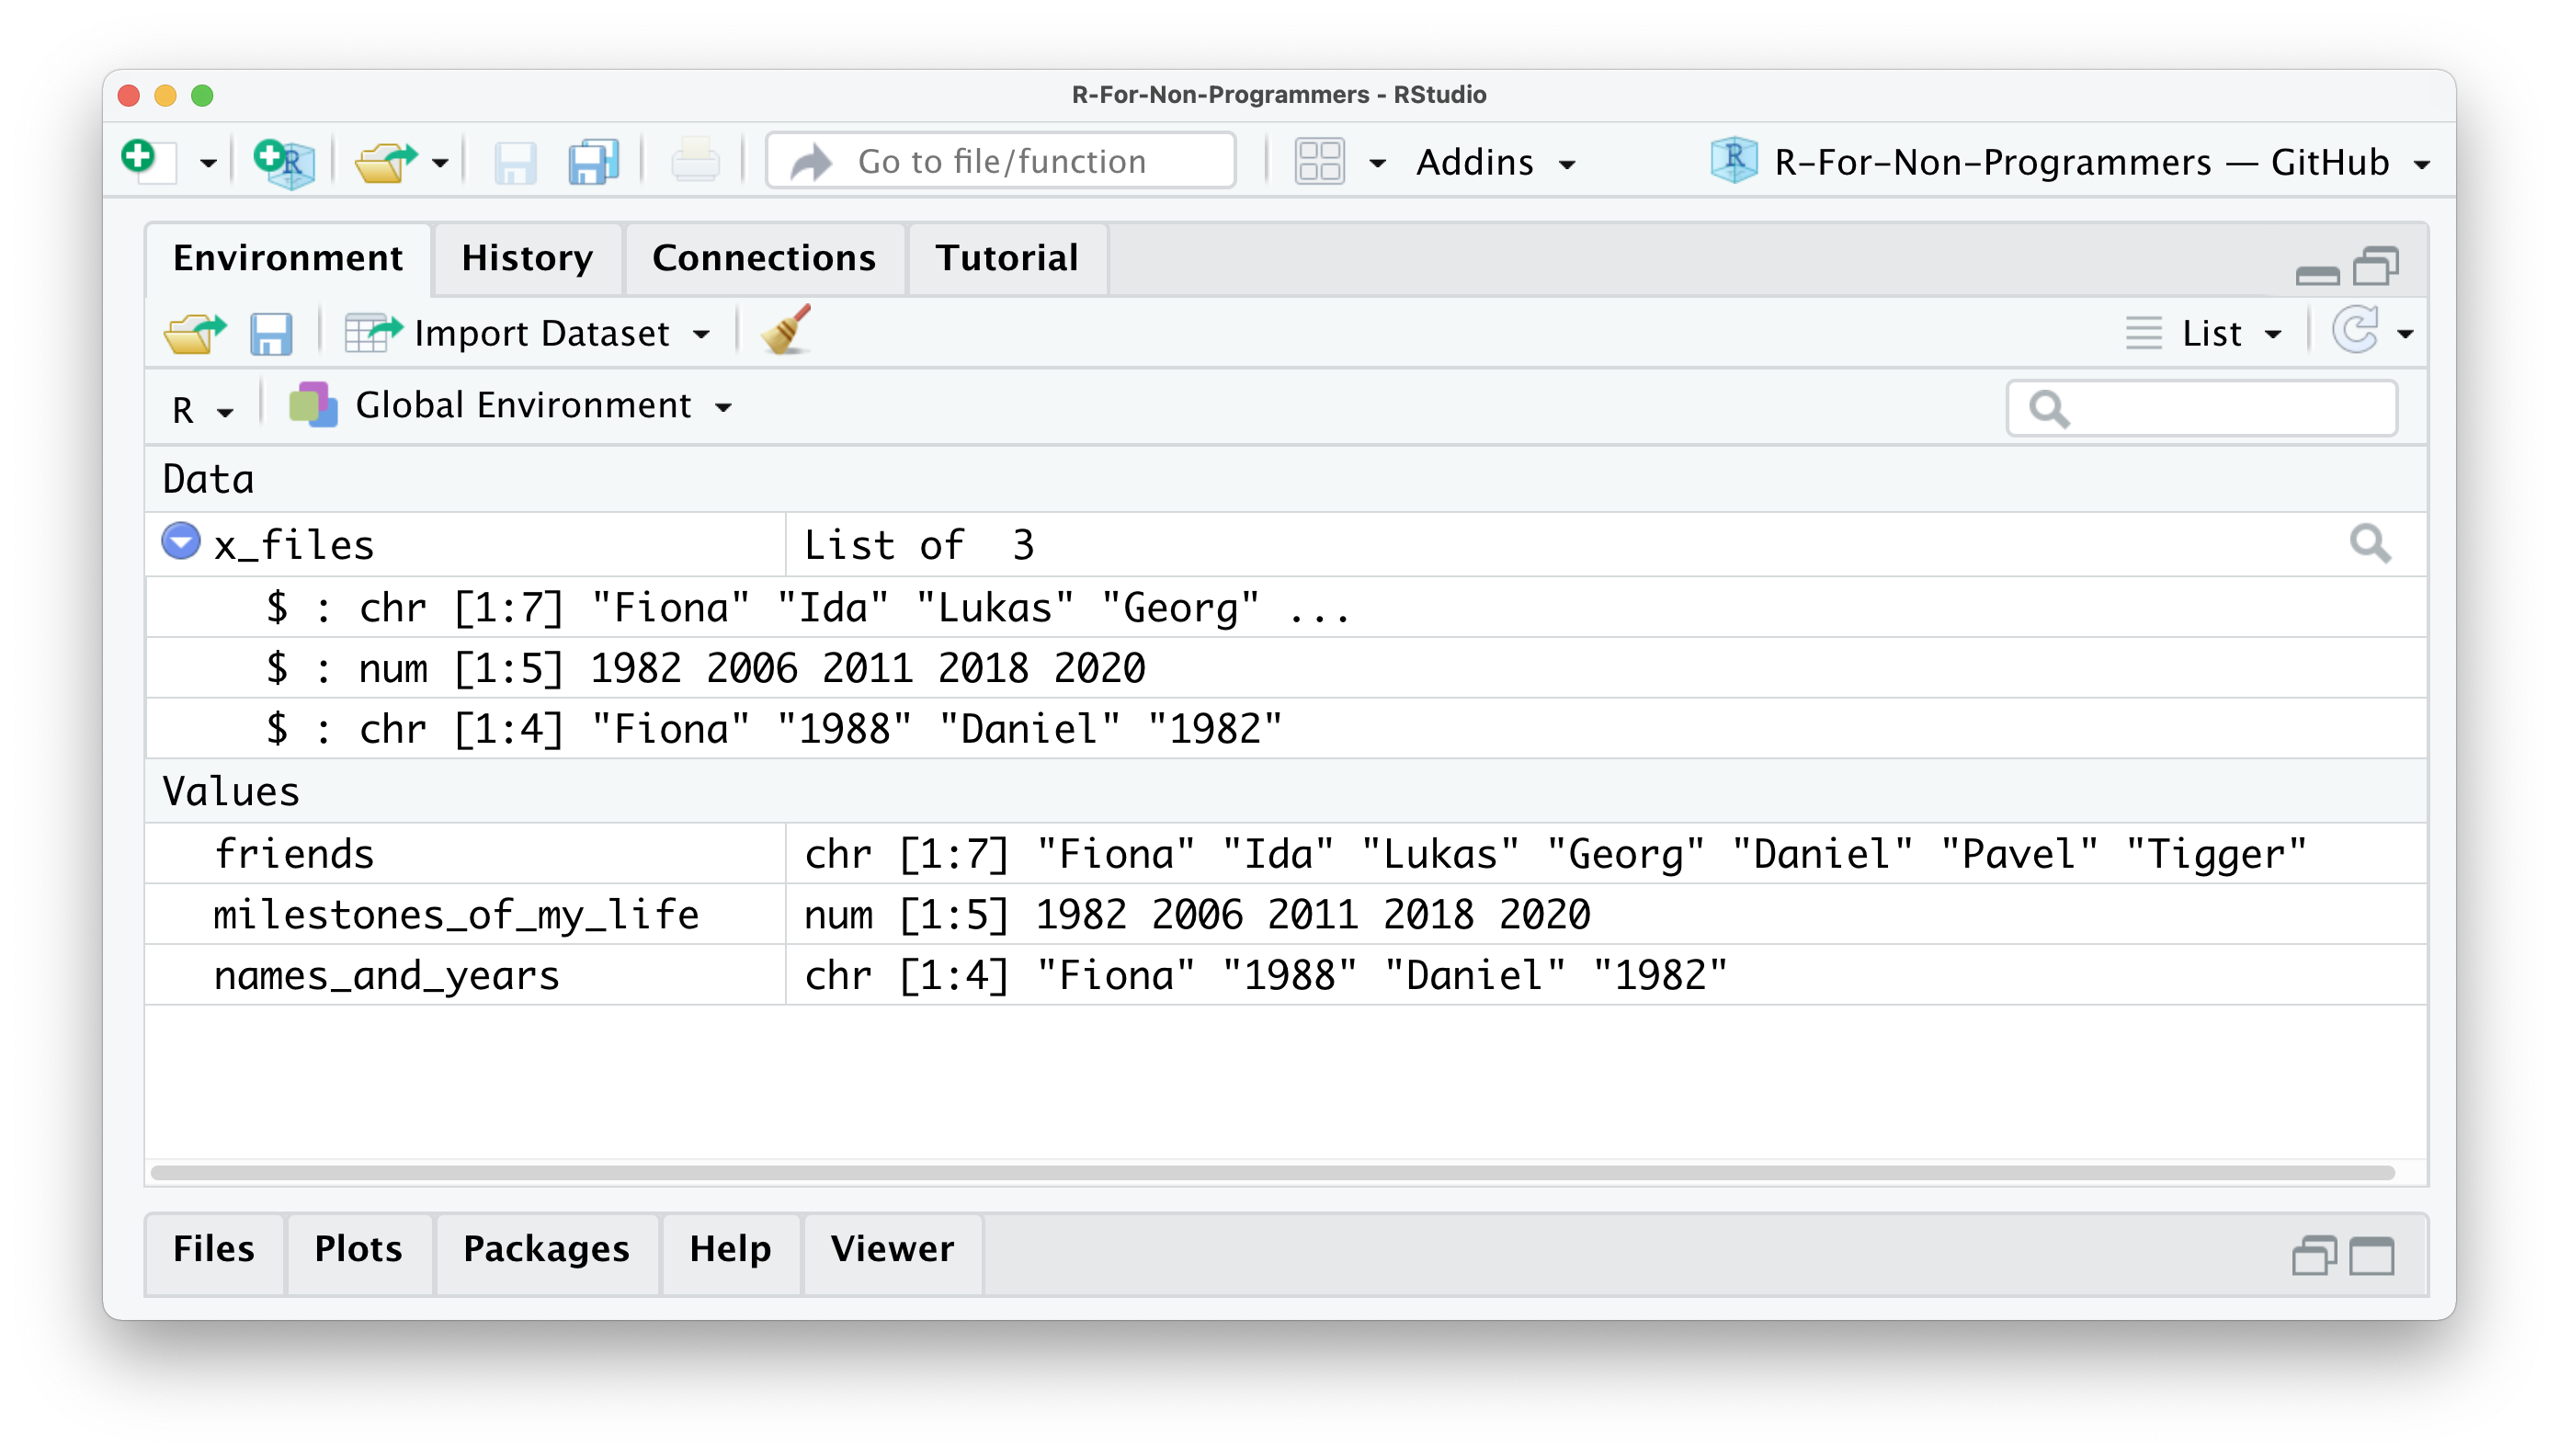
\includegraphics{images/chapter_05_img/02_basic_computation_environment_lists.png}

}

\caption{\label{fig-img-x-files}The environment pane showing our objects
and our list \texttt{x\_files}}

\end{figure}%

In Chapter (\textbf{basic-computations-in-r?}) , I mentioned that we
should avoid using the \texttt{=} operator and explained that it is used
to assign values to objects. You can, if you want, use \texttt{=}
instead of \texttt{\textless{}-}. They fulfil the same purpose. However,
as mentioned before, it is not wise to do so. Here is an example that
shows that, in principle, it is possible.

\begin{Shaded}
\begin{Highlighting}[]
\CommentTok{\# DO}
\NormalTok{(avengers1 }\OtherTok{\textless{}{-}} \FunctionTok{c}\NormalTok{(}\StringTok{"Iron Man"}\NormalTok{,}
                \StringTok{"Captain America"}\NormalTok{,}
                \StringTok{"Black Widow"}\NormalTok{,}
                \StringTok{"Vision"}\NormalTok{))}
\end{Highlighting}
\end{Shaded}

\begin{verbatim}
[1] "Iron Man"        "Captain America" "Black Widow"     "Vision"         
\end{verbatim}

\begin{Shaded}
\begin{Highlighting}[]
\CommentTok{\# DON\textquotesingle{}T}
\NormalTok{(}\AttributeTok{avengers2 =} \FunctionTok{c}\NormalTok{(}\StringTok{"Iron Man"}\NormalTok{,}
               \StringTok{"Captain America"}\NormalTok{,}
               \StringTok{"Black Widow"}\NormalTok{,}
               \StringTok{"Vision"}\NormalTok{))}
\end{Highlighting}
\end{Shaded}

\begin{verbatim}
[1] "Iron Man"        "Captain America" "Black Widow"     "Vision"         
\end{verbatim}

On a final note, naming your objects is limited. You cannot chose any
name. First, every name needs to start with a letter. Second, you can
only use letters, numbers \texttt{\_} and \texttt{.} as valid components
of the names for your objects (see also Chapter 4.2 in Wickham and
Grolemund 2016). I recommend to establish a naming convention that you
adhere to. Personally I prefer to only user lower-case letters and
\texttt{\_} to separate/connect words. Ideally, you want to keep names
informative, succinct and precise. Here are some examples of what some
might consider good and bad choices for names.

\begin{Shaded}
\begin{Highlighting}[]
\CommentTok{\# Good choices}
\NormalTok{income\_per\_annum}
\NormalTok{open\_to\_exp          }\CommentTok{\# for \textquotesingle{}openness to new experiences\textquotesingle{}}
\NormalTok{soc\_int              }\CommentTok{\# for \textquotesingle{}social integration\textquotesingle{}}
 
\CommentTok{\# Bad choices}
\NormalTok{IncomePerAnnum}
\NormalTok{measurement\_of\_boredom\_of\_watching\_youtube}
\NormalTok{Sleep.per\_monthsIn.hours}
\end{Highlighting}
\end{Shaded}

Ultimately, you need to be able to effectively work with your data and
output. Ideally, this should be true for others as well who want or need
to work with your analysis and data as well, e.g.~your co-investigator
or supervisor. The same is applies to column names in datasets (see
Chapter @ref(colnames-cleaning)). Some more information about coding
style and coding etiquette can be found in Chapter
@ref(coding-etiquette).

\section{Functions}\label{functions}

I used the term `\emph{function}' multiple times, but I never thoroughly
explained what they are and why we need them. In simple terms, functions
are objects. They contain lines of code that someone has written for us
or we have written ourselves. One could say they are code snippets ready
to use. Someone else might see them as shortcuts for our programming.
Functions increase the speed with which we perform our analysis and
write our computations and make our code more readable and reliable.
Consider computing the \texttt{mean} of values stored in the object
\texttt{pocket\_money}.

\begin{Shaded}
\begin{Highlighting}[]
\CommentTok{\# First we create an object that stores our desired values}
\NormalTok{pocket\_money }\OtherTok{\textless{}{-}} \FunctionTok{c}\NormalTok{(}\DecValTok{0}\NormalTok{, }\DecValTok{1}\NormalTok{, }\DecValTok{1}\NormalTok{, }\DecValTok{2}\NormalTok{, }\DecValTok{3}\NormalTok{, }\DecValTok{5}\NormalTok{, }\DecValTok{8}\NormalTok{, }\DecValTok{13}\NormalTok{, }\DecValTok{21}\NormalTok{, }\DecValTok{34}\NormalTok{, }\DecValTok{55}\NormalTok{, }\DecValTok{89}\NormalTok{)}

\CommentTok{\#1 Manually compute the mean}
\NormalTok{sum }\OtherTok{\textless{}{-}} \DecValTok{0} \SpecialCharTok{+} \DecValTok{1} \SpecialCharTok{+} \DecValTok{1} \SpecialCharTok{+} \DecValTok{2} \SpecialCharTok{+} \DecValTok{3} \SpecialCharTok{+} \DecValTok{5} \SpecialCharTok{+} \DecValTok{8} \SpecialCharTok{+} \DecValTok{13} \SpecialCharTok{+} \DecValTok{21} \SpecialCharTok{+} \DecValTok{34} \SpecialCharTok{+} \DecValTok{55} \SpecialCharTok{+} \DecValTok{89}
\NormalTok{sum }\SpecialCharTok{/} \DecValTok{12} \CommentTok{\# There are 12 items in the object}
\end{Highlighting}
\end{Shaded}

\begin{verbatim}
[1] 19.33333
\end{verbatim}

\begin{Shaded}
\begin{Highlighting}[]
\CommentTok{\#2 Use a function to compute the mean}
\FunctionTok{mean}\NormalTok{(pocket\_money)}
\end{Highlighting}
\end{Shaded}

\begin{verbatim}
[1] 19.33333
\end{verbatim}

\begin{Shaded}
\begin{Highlighting}[]
\CommentTok{\#3 Let\textquotesingle{}s make sure \#1 and \#2 are actually the same}
\NormalTok{sum }\SpecialCharTok{/} \DecValTok{12} \SpecialCharTok{==} \FunctionTok{mean}\NormalTok{(pocket\_money)}
\end{Highlighting}
\end{Shaded}

\begin{verbatim}
[1] TRUE
\end{verbatim}

If we manually compute the mean, we first calculate the sum of all
values in the object \texttt{pocket\_money}\footnote{If you find the
  order of numbers suspicious, it is because it represents the famous
  \href{https://en.wikipedia.org/wiki/Fibonacci_number}{Fibonacci
  sequence}.}. Then we divide it by the number of values in the object,
which is \texttt{12}. This is the traditional way of computing the mean
as we know it from primary school. However, by simply using the function
\texttt{mean()}, we not only write considerably less code, but it is
also much easier to understand because the word \emph{`mean'} does
precisely what we would expect. Which approach do you find easier: Using
the function \texttt{mean()} or compute it by hand?

To further illustrate how functions look like, let's create one
ourselves and call it \texttt{my\_mean}.

\begin{Shaded}
\begin{Highlighting}[]
\NormalTok{my\_mean }\OtherTok{\textless{}{-}} \ControlFlowTok{function}\NormalTok{(numbers)\{}
  \CommentTok{\# Compute the sum of all values in \textquotesingle{}numbers\textquotesingle{}}
\NormalTok{  sum }\OtherTok{\textless{}{-}} \FunctionTok{sum}\NormalTok{(numbers)}
  
  \CommentTok{\# Divide the sum by the number of items in \textquotesingle{}numbers\textquotesingle{}}
\NormalTok{  result }\OtherTok{\textless{}{-}}\NormalTok{ sum}\SpecialCharTok{/}\FunctionTok{length}\NormalTok{(numbers)}
  
  \CommentTok{\# Return the result in the console}
  \FunctionTok{return}\NormalTok{(result)}
\NormalTok{\}}

\FunctionTok{my\_mean}\NormalTok{(pocket\_money)}
\end{Highlighting}
\end{Shaded}

\begin{verbatim}
[1] 19.33333
\end{verbatim}

Don't worry if half of this code does not make sense to you. Writing
functions is an advanced \emph{R} skill. However, it is good to know how
functions look on the `inside'. You certainly can see the similarities
between the code we have written before, but instead of using actual
numbers, we work with placeholders like \texttt{numbers}. This way, we
can use a function for different data and do not have to rewrite it
every time. Writing and using functions relates to the skill of
abstraction mentioned in Chapter
@ref(programming-languages-enhance-your-conceptual-thinking).

All functions in \emph{R} share the same structure. They have a
\texttt{name} followed by \texttt{()}. Within these parentheses, we put
\texttt{arguments}, which have specific \texttt{values}. For example, a
generic structure of a function would look something like this:

\begin{Shaded}
\begin{Highlighting}[]
\FunctionTok{name\_of\_function}\NormalTok{(}\AttributeTok{argument\_1 =}\NormalTok{ value\_1,}
                 \AttributeTok{argument\_2 =}\NormalTok{ value\_2,}
                 \AttributeTok{argument\_3 =}\NormalTok{ value\_3)}
\end{Highlighting}
\end{Shaded}

How many arguments there are and what kind of values you can provide is
very much dependent on the function you use. Thus, not every function
takes every value. In the case of \texttt{mean()}, the function takes an
object which holds a sequence of \texttt{numeric} values. It would make
very little sense to compute the mean of our \texttt{friends} object,
because it only contains names. \emph{R} would return an error message:

\begin{Shaded}
\begin{Highlighting}[]
\FunctionTok{mean}\NormalTok{(friends)}
\end{Highlighting}
\end{Shaded}

\begin{verbatim}
Warning in mean.default(friends): argument is not numeric or logical: returning
NA
\end{verbatim}

\begin{verbatim}
[1] NA
\end{verbatim}

\texttt{NA} refers to a value that is \emph{`not available'}. In this
case, \emph{R} tries to compute the mean, but the result is not
available, because the values are not \texttt{numeric} but a
\texttt{character}. In your dataset, you might find values that are
\texttt{NA}, which means there is data missing. If a function attempts a
computation that includes even just a single value that is \texttt{NA},
\emph{R} will return \texttt{NA}. However, there is a way to fix this.
You will learn more about how to deal with \texttt{NA} values in Chapter
@ref(dealing-with-missing-data).

Sometimes you will also get a message from \emph{R} that states
\texttt{NaN}. \texttt{NaN} stands for \emph{`not a number'} and is
returned when something is not possible to compute, for example:

\begin{Shaded}
\begin{Highlighting}[]
\CommentTok{\# Example 1}
\DecValTok{0} \SpecialCharTok{/} \DecValTok{0}
\end{Highlighting}
\end{Shaded}

\begin{verbatim}
[1] NaN
\end{verbatim}

\begin{Shaded}
\begin{Highlighting}[]
\CommentTok{\# Example 2}
\FunctionTok{sqrt}\NormalTok{(}\SpecialCharTok{{-}}\DecValTok{9}\NormalTok{)}
\end{Highlighting}
\end{Shaded}

\begin{verbatim}
Warning in sqrt(-9): NaNs produced
\end{verbatim}

\begin{verbatim}
[1] NaN
\end{verbatim}

\section{R packages}\label{r-packages}

\emph{R} has many built-in functions that we can use right away.
However, some of the most interesting ones are developed by different
programmers, data scientists and enthusiasts. To add more functions to
your repertoire, you can install \emph{R} packages. \emph{R} packages
are a collection of functions that you can download and use for your own
analysis. Throughout this book, you will learn about and use many
different \emph{R} packages to accomplish various tasks. To give you
another analogy,

\begin{itemize}
\item
  \emph{R} is like a global supermarket where everyone can offer their
  products,
\item
  RStudio is like my shopping cart where I can put the products I like,
  and
\item
  \emph{R} packages are the products I can pick from the shelves.
\end{itemize}

Luckily, \emph{R} packages are free to use, so I do not have to bring my
credit card. For me, these additional functions, developed by some of
the most outstanding scientists, is one of many reasons that keeps me
addicted to performing my research in \emph{R}.

\emph{R} packages do not only include functions but often include
datasets and documentation of what each function does. This way, you can
easily try every function right away, even without your own dataset and
read through what each function in the package does.
Figure~\ref{fig-img-r-package-documentation} shows the documentation of
an \emph{R} package called \texttt{ggplot2}.

\begin{figure}

\centering{

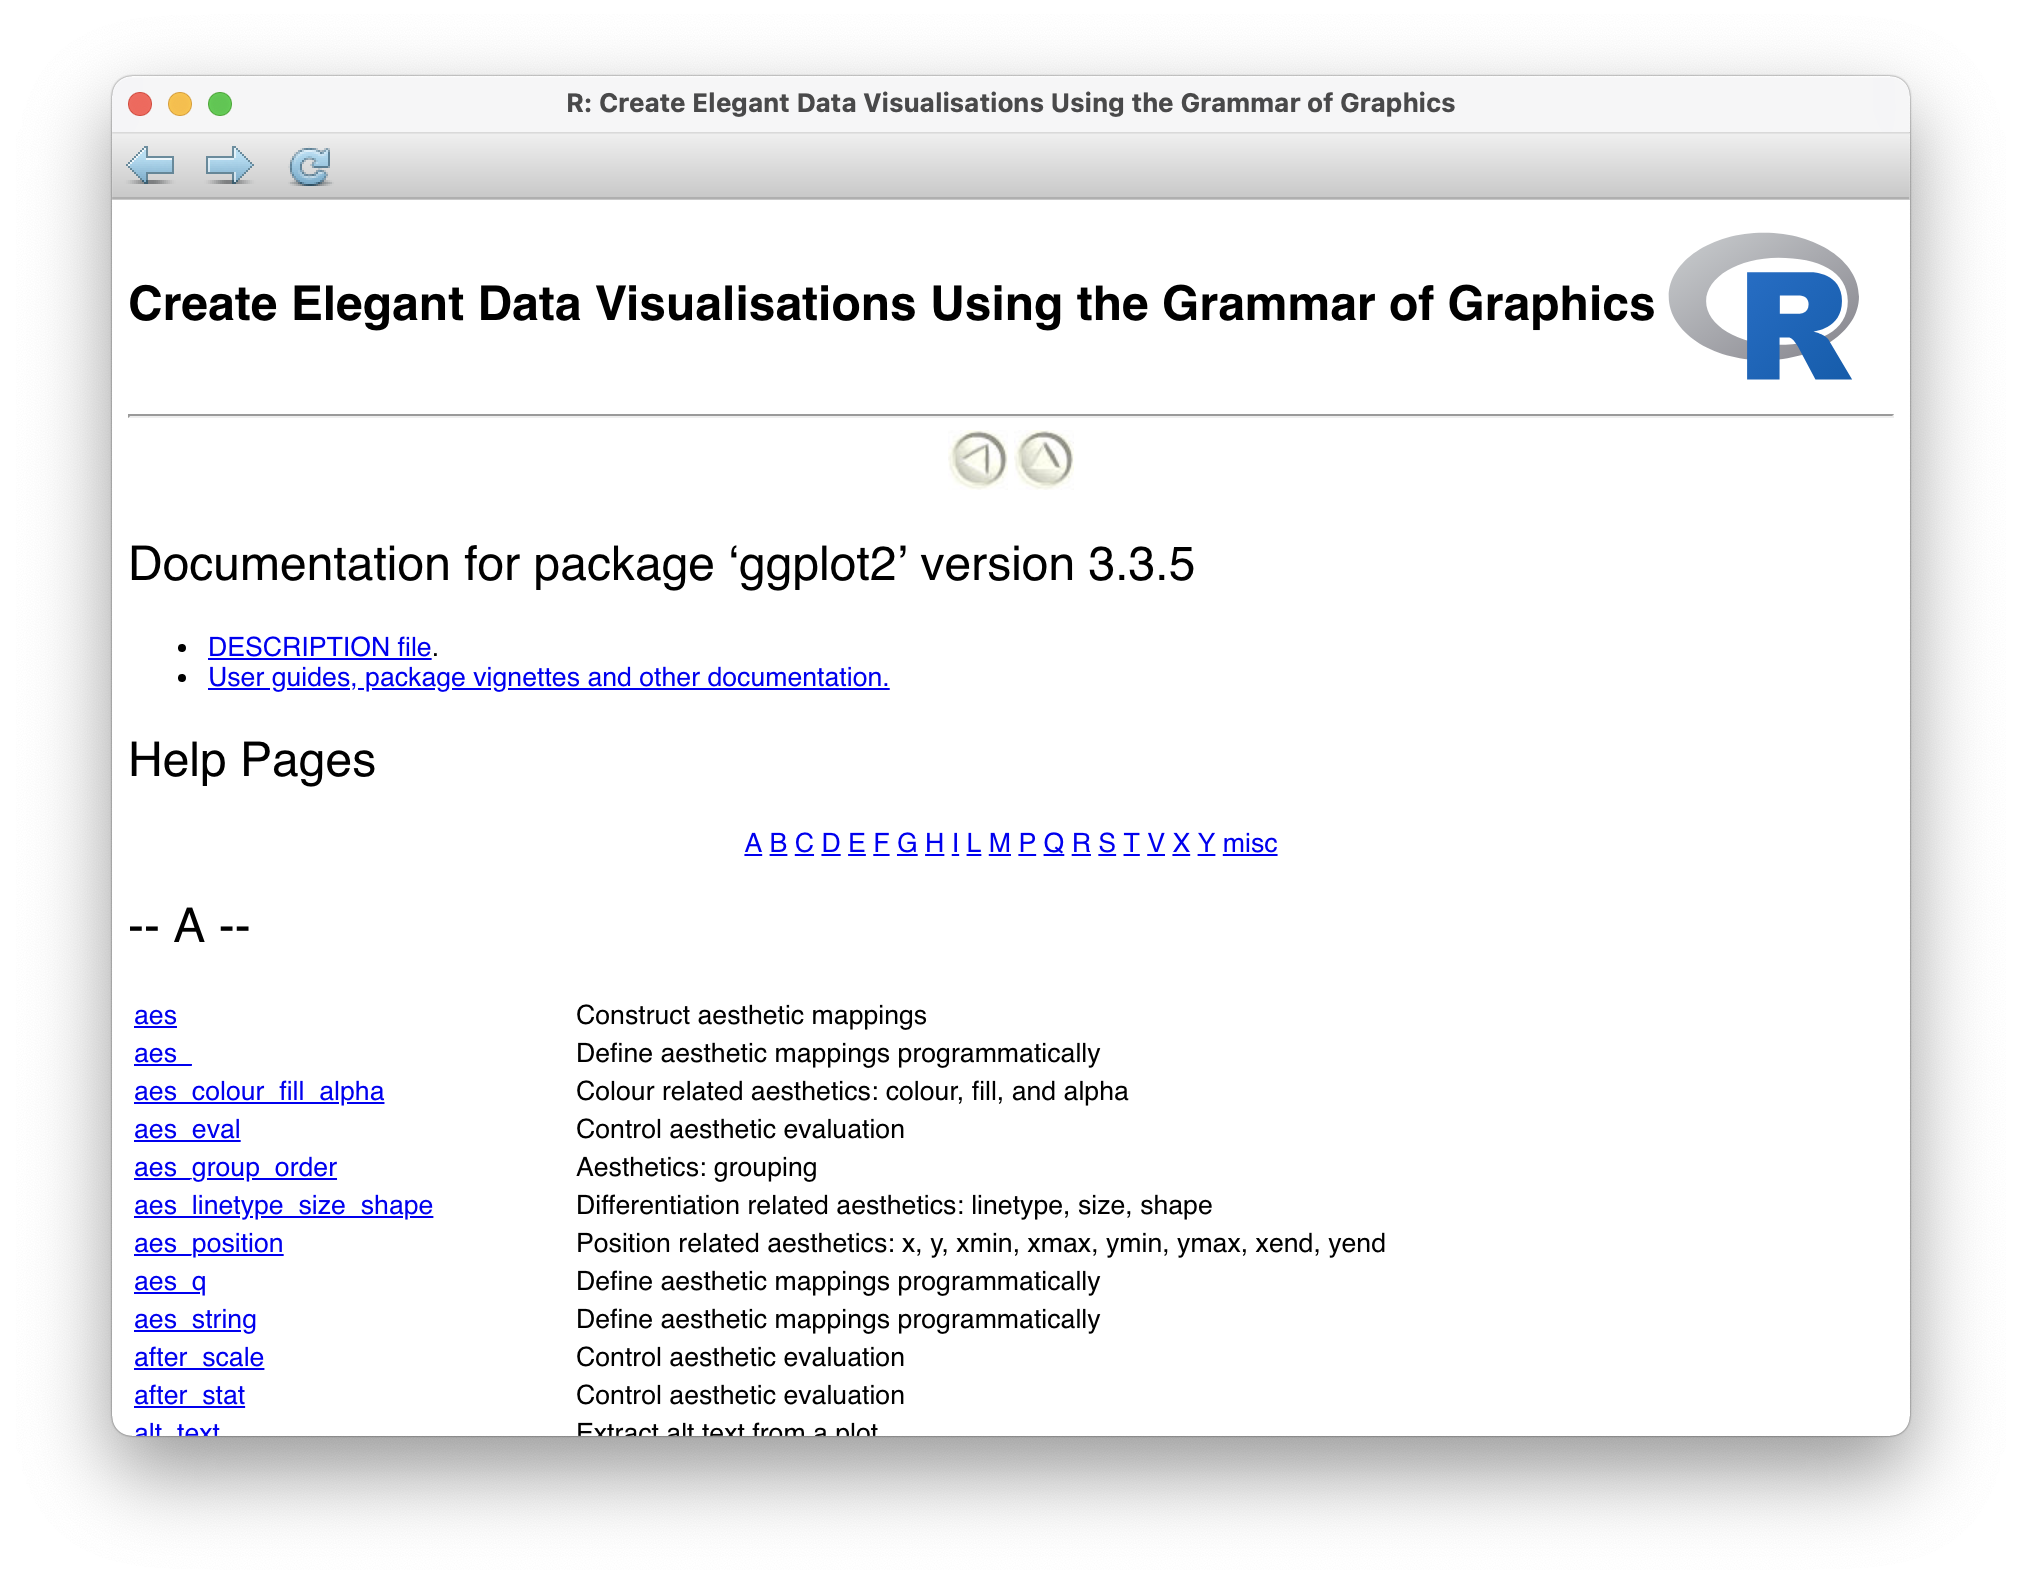
\includegraphics{images/chapter_05_img/r_package_documentation.png}

}

\caption{\label{fig-img-r-package-documentation}The R package
documentation for `ggplot2'}

\end{figure}%

However, how do you find those \emph{R} packages? They are right at your
fingertips. You have two options:

\begin{enumerate}
\def\labelenumi{\arabic{enumi}.}
\item
  Use the function \texttt{install.packages()}, or
\item
  Use the packages pane in RStudio.
\end{enumerate}

\subsection{\texorpdfstring{Installing packages using
\texttt{install.packages()}}{Installing packages using install.packages()}}\label{installing-packages-using-a-function}

The simplest and fastest way to install a package is calling the
function \texttt{install.packages()}. You can either use it to install a
single package or install a series of packages all at once using our
trusty \texttt{c()} function. All you need to know is the name of the
package. This approach works for all packages that are on CRAN (remember
CRAN from Chapter @ref(installing-r)?).

\begin{Shaded}
\begin{Highlighting}[]
\CommentTok{\# Install a single package}
\FunctionTok{install.packages}\NormalTok{(}\StringTok{"tidyverse"}\NormalTok{)}

\CommentTok{\# Install multiple packages at once}
\FunctionTok{install.packages}\NormalTok{(}\FunctionTok{c}\NormalTok{(}\StringTok{"tidyverse"}\NormalTok{, }\StringTok{"naniar"}\NormalTok{, }\StringTok{"psych"}\NormalTok{))}
\end{Highlighting}
\end{Shaded}

If a package is not available from CRAN, chances are you can find them
on \href{https://github.com}{GitHub}. GitHub is probably the world's
largest global platform for programmers from all walks of life, and many
of them develop fantastic \emph{R} packages that make programming and
data analysis not just easier but a lot more fun. As you continue to
work in \emph{R}, you should seriously consider creating your own
account to keep backups of your projects (see also Chapter
@ref(next-steps-github)).

An essential companion for this book is \texttt{r4np}, which contains
all datasets for this book and some useful functions to get you up and
running in no time. Since it is currently only available on Github, you
can use the following code snippet to install it. However, you have to
install the package \texttt{devtools} first to use the function
\texttt{install\_github()}.

\begin{Shaded}
\begin{Highlighting}[]
\CommentTok{\# Install the \textquotesingle{}devtools\textquotesingle{} package first}
\FunctionTok{install.packages}\NormalTok{(}\StringTok{"devtools"}\NormalTok{)}

\CommentTok{\# Then install the \textquotesingle{}r4np\textquotesingle{} package from GitHub}
\NormalTok{devtools}\SpecialCharTok{::}\FunctionTok{install\_github}\NormalTok{(}\StringTok{"ddauber/r4np"}\NormalTok{)}
\end{Highlighting}
\end{Shaded}

\subsection{Installing packages via RStudio's package
pane}\label{installing-packages-via-rstudio}

RStudio offers a very convenient way of installing packages. In the
packages pane, you cannot only see your installed packages, but you have
two more buttons: \texttt{Install} and \texttt{Update}. The names are
very self-explanatory. To install an \emph{R} package you can follow the
following steps:

\begin{enumerate}
\def\labelenumi{\arabic{enumi}.}
\item
  Click on \texttt{Install}.
\item
  In most cases, you want to make sure you have
  \texttt{Repository\ (CRAN)} selected.

  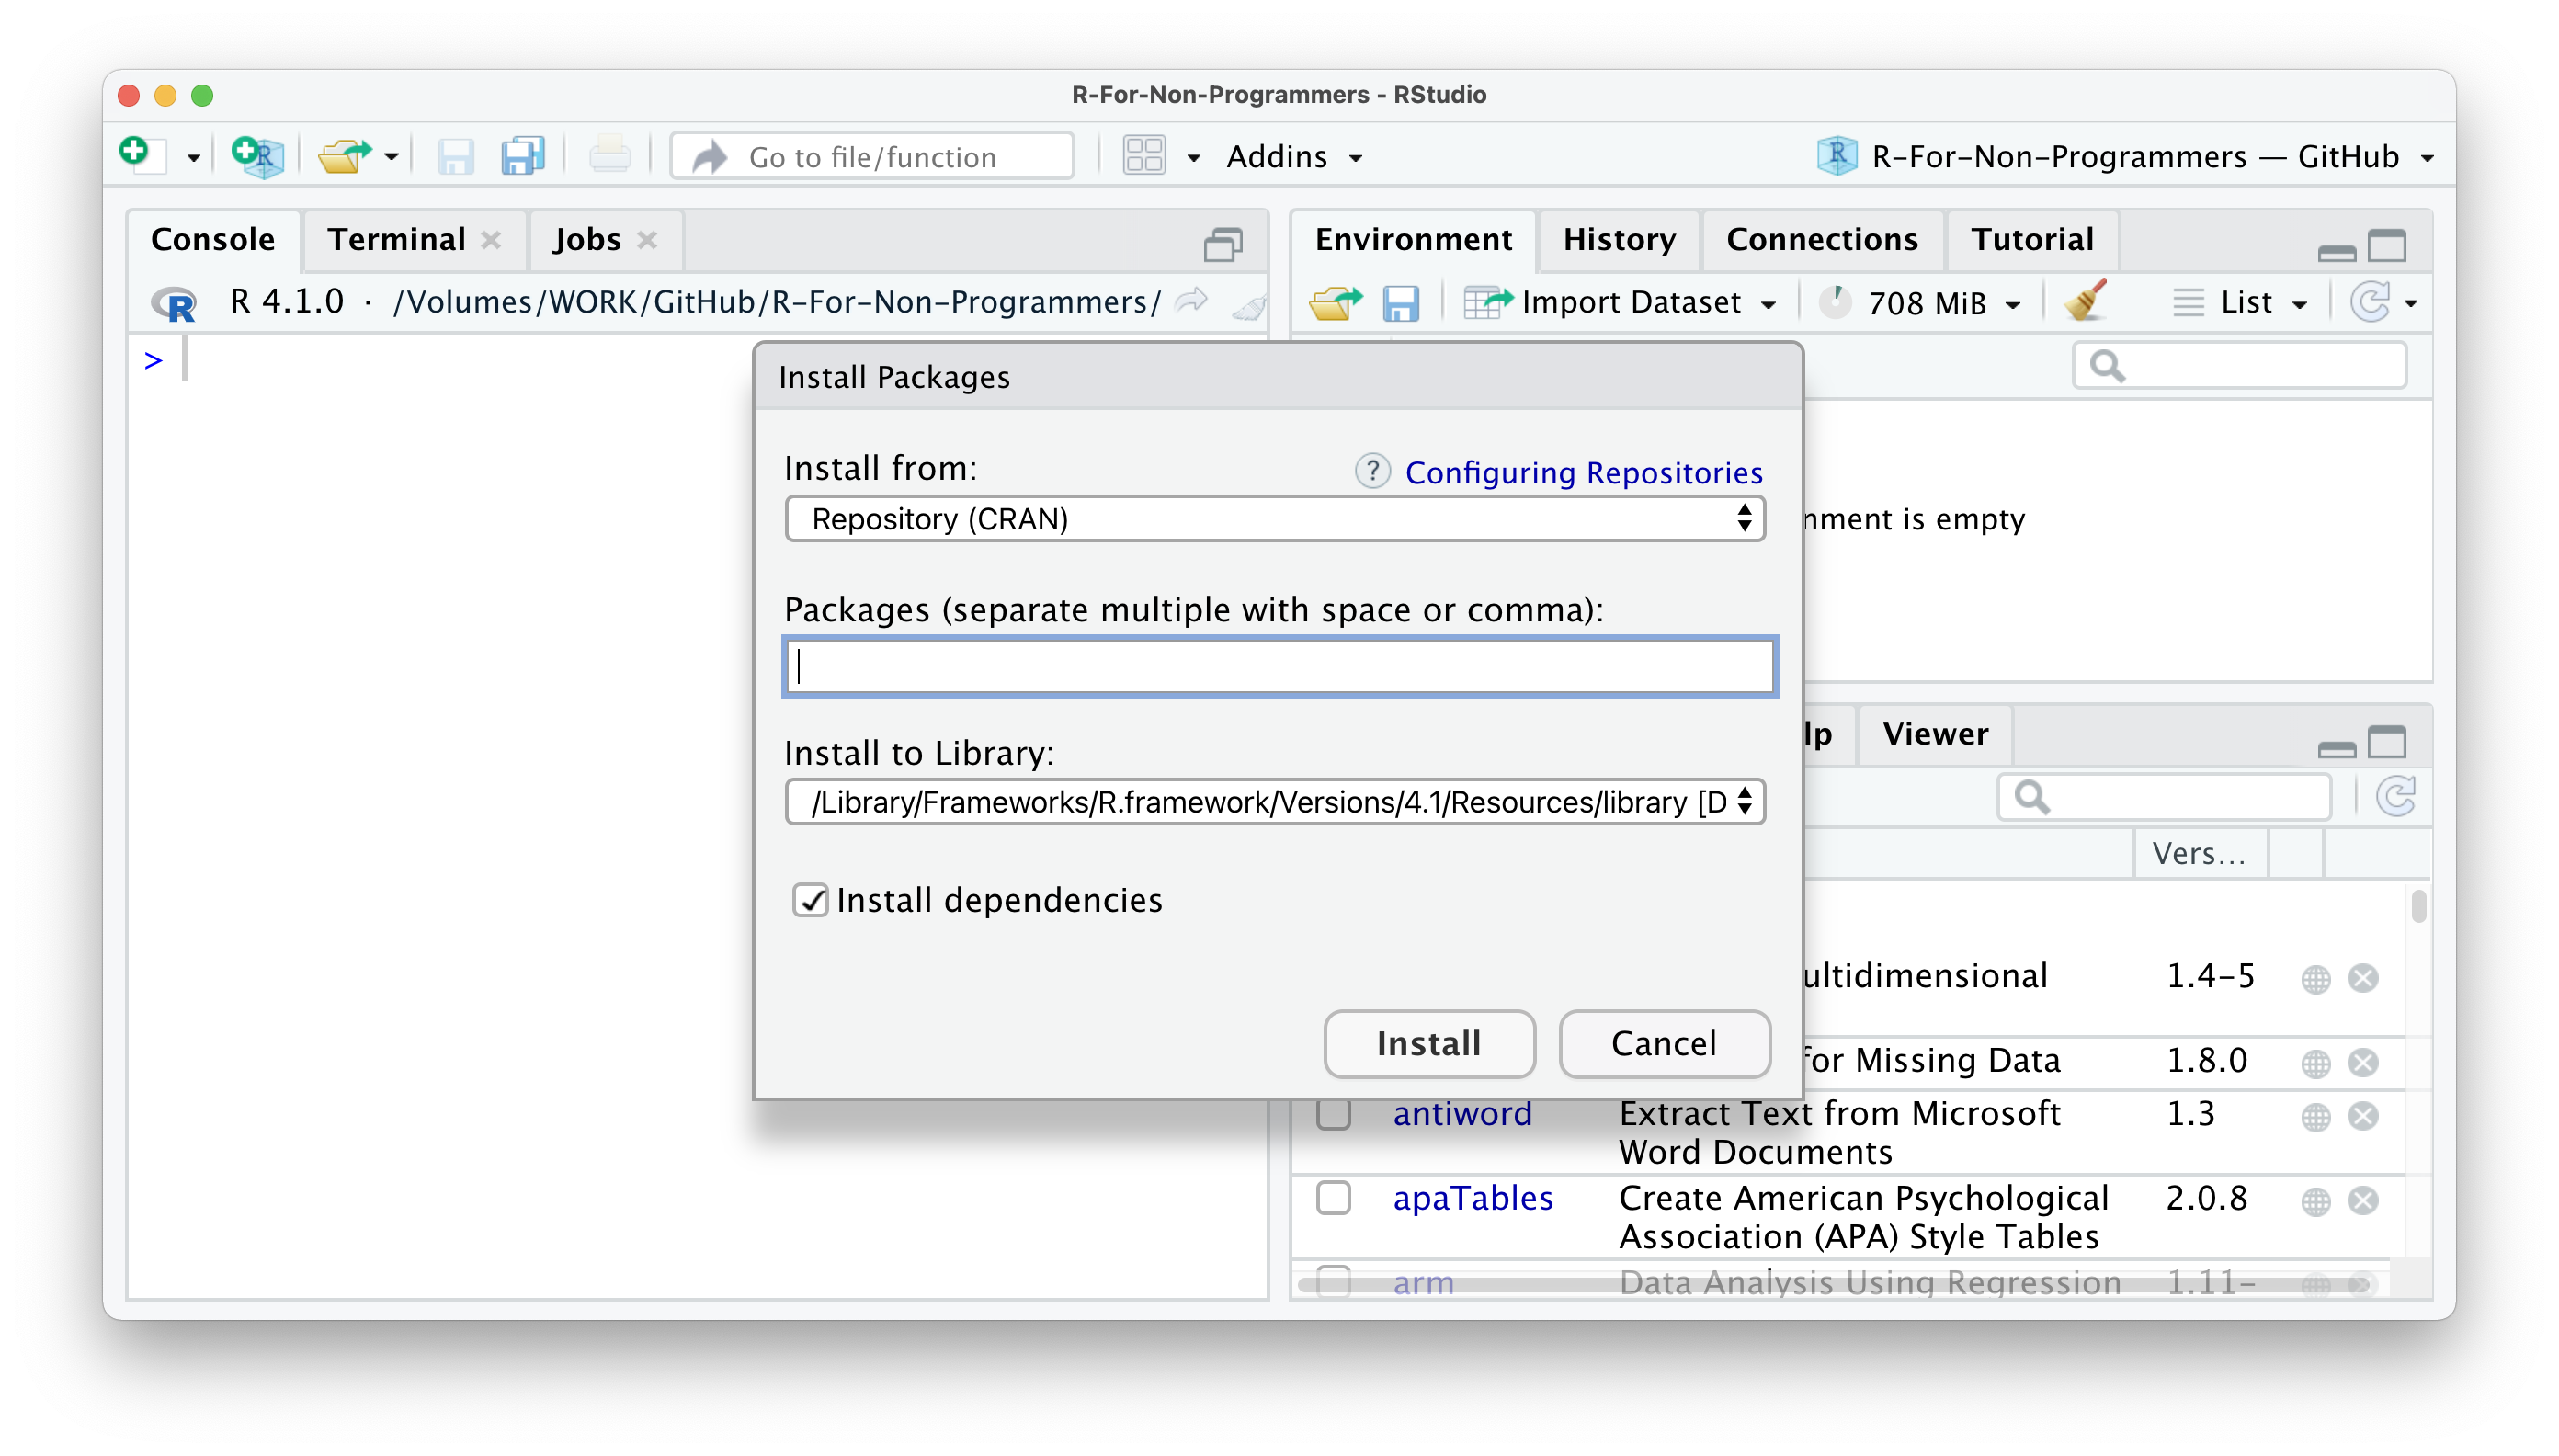
\includegraphics{images/chapter_05_img/install_r_packages/01_install_r_packages.png}
\item
  Type in the name of the package you wish to install. RStudio offers an
  auto-complete feature to make it even easier to find the package you
  want.

  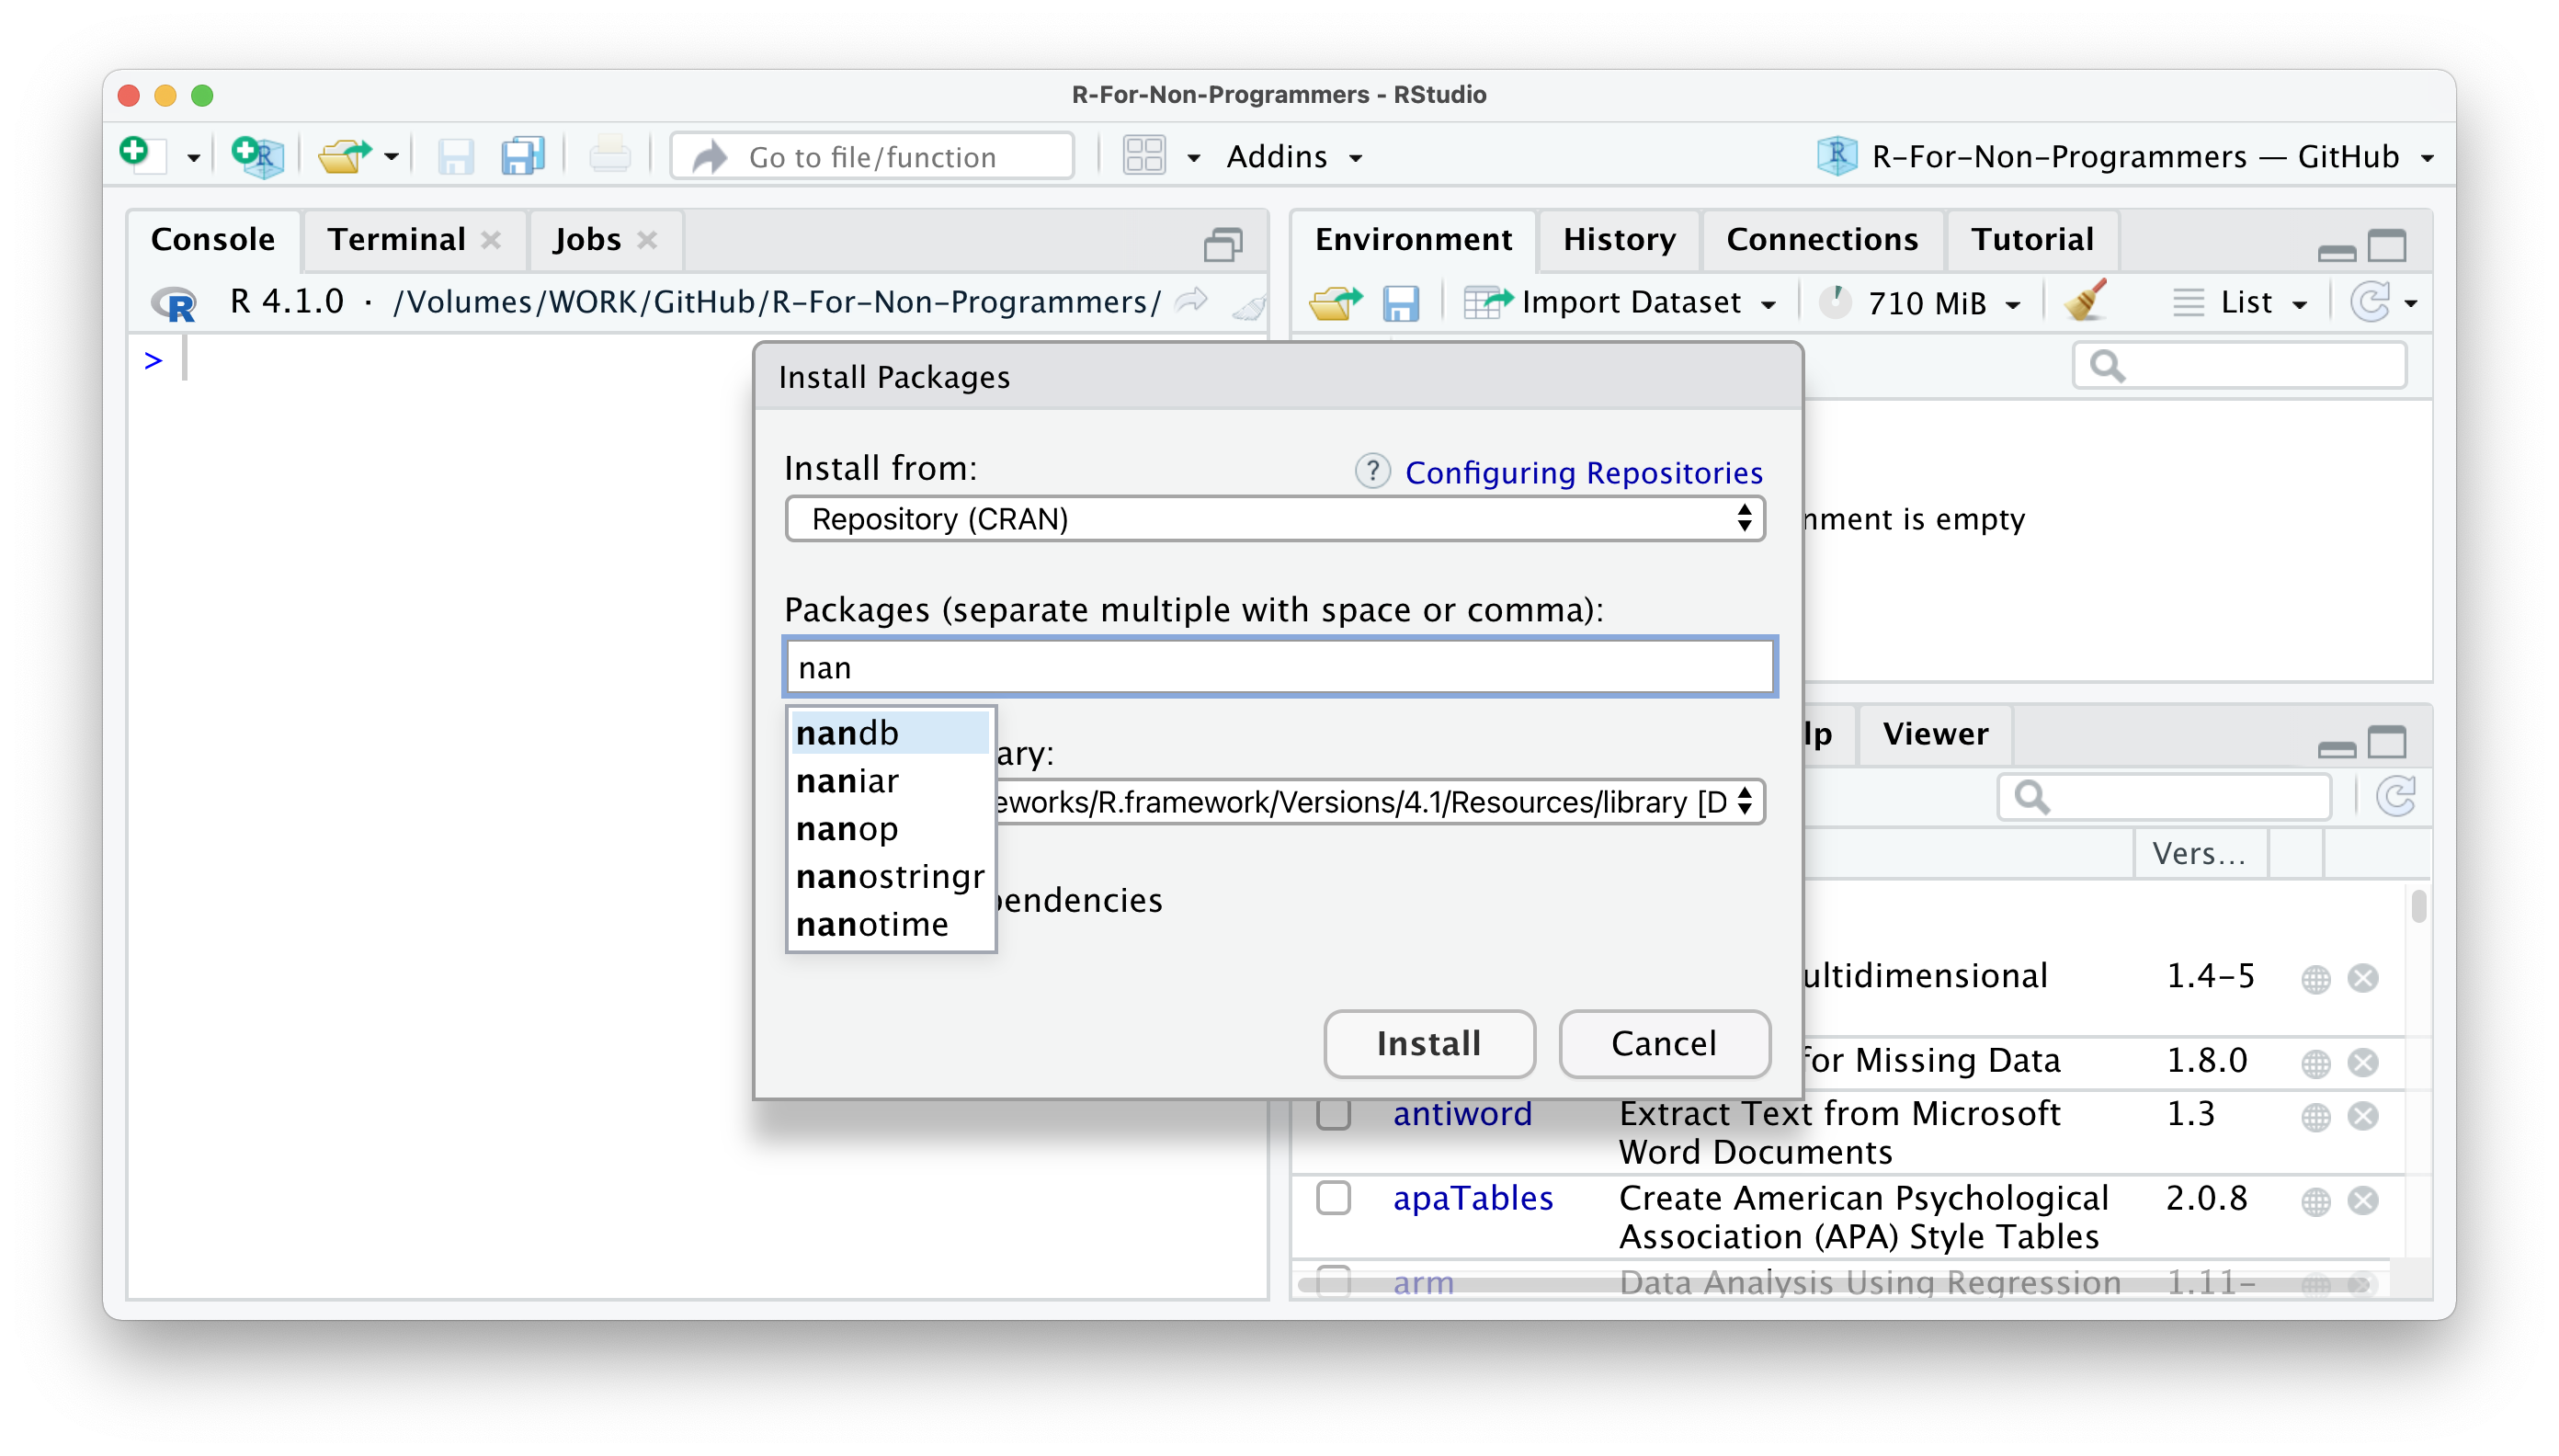
\includegraphics{images/chapter_05_img/install_r_packages/02_install_r_packages.png}
\item
  I recommend NOT to change the option which says
  \texttt{Install\ to\ library}. The default library settings will
  suffice.
\item
  Finally, I recommend to select \texttt{Install\ dependencies}, because
  some packages need other packages to function properly. This way, you
  do not have to do this manually.

  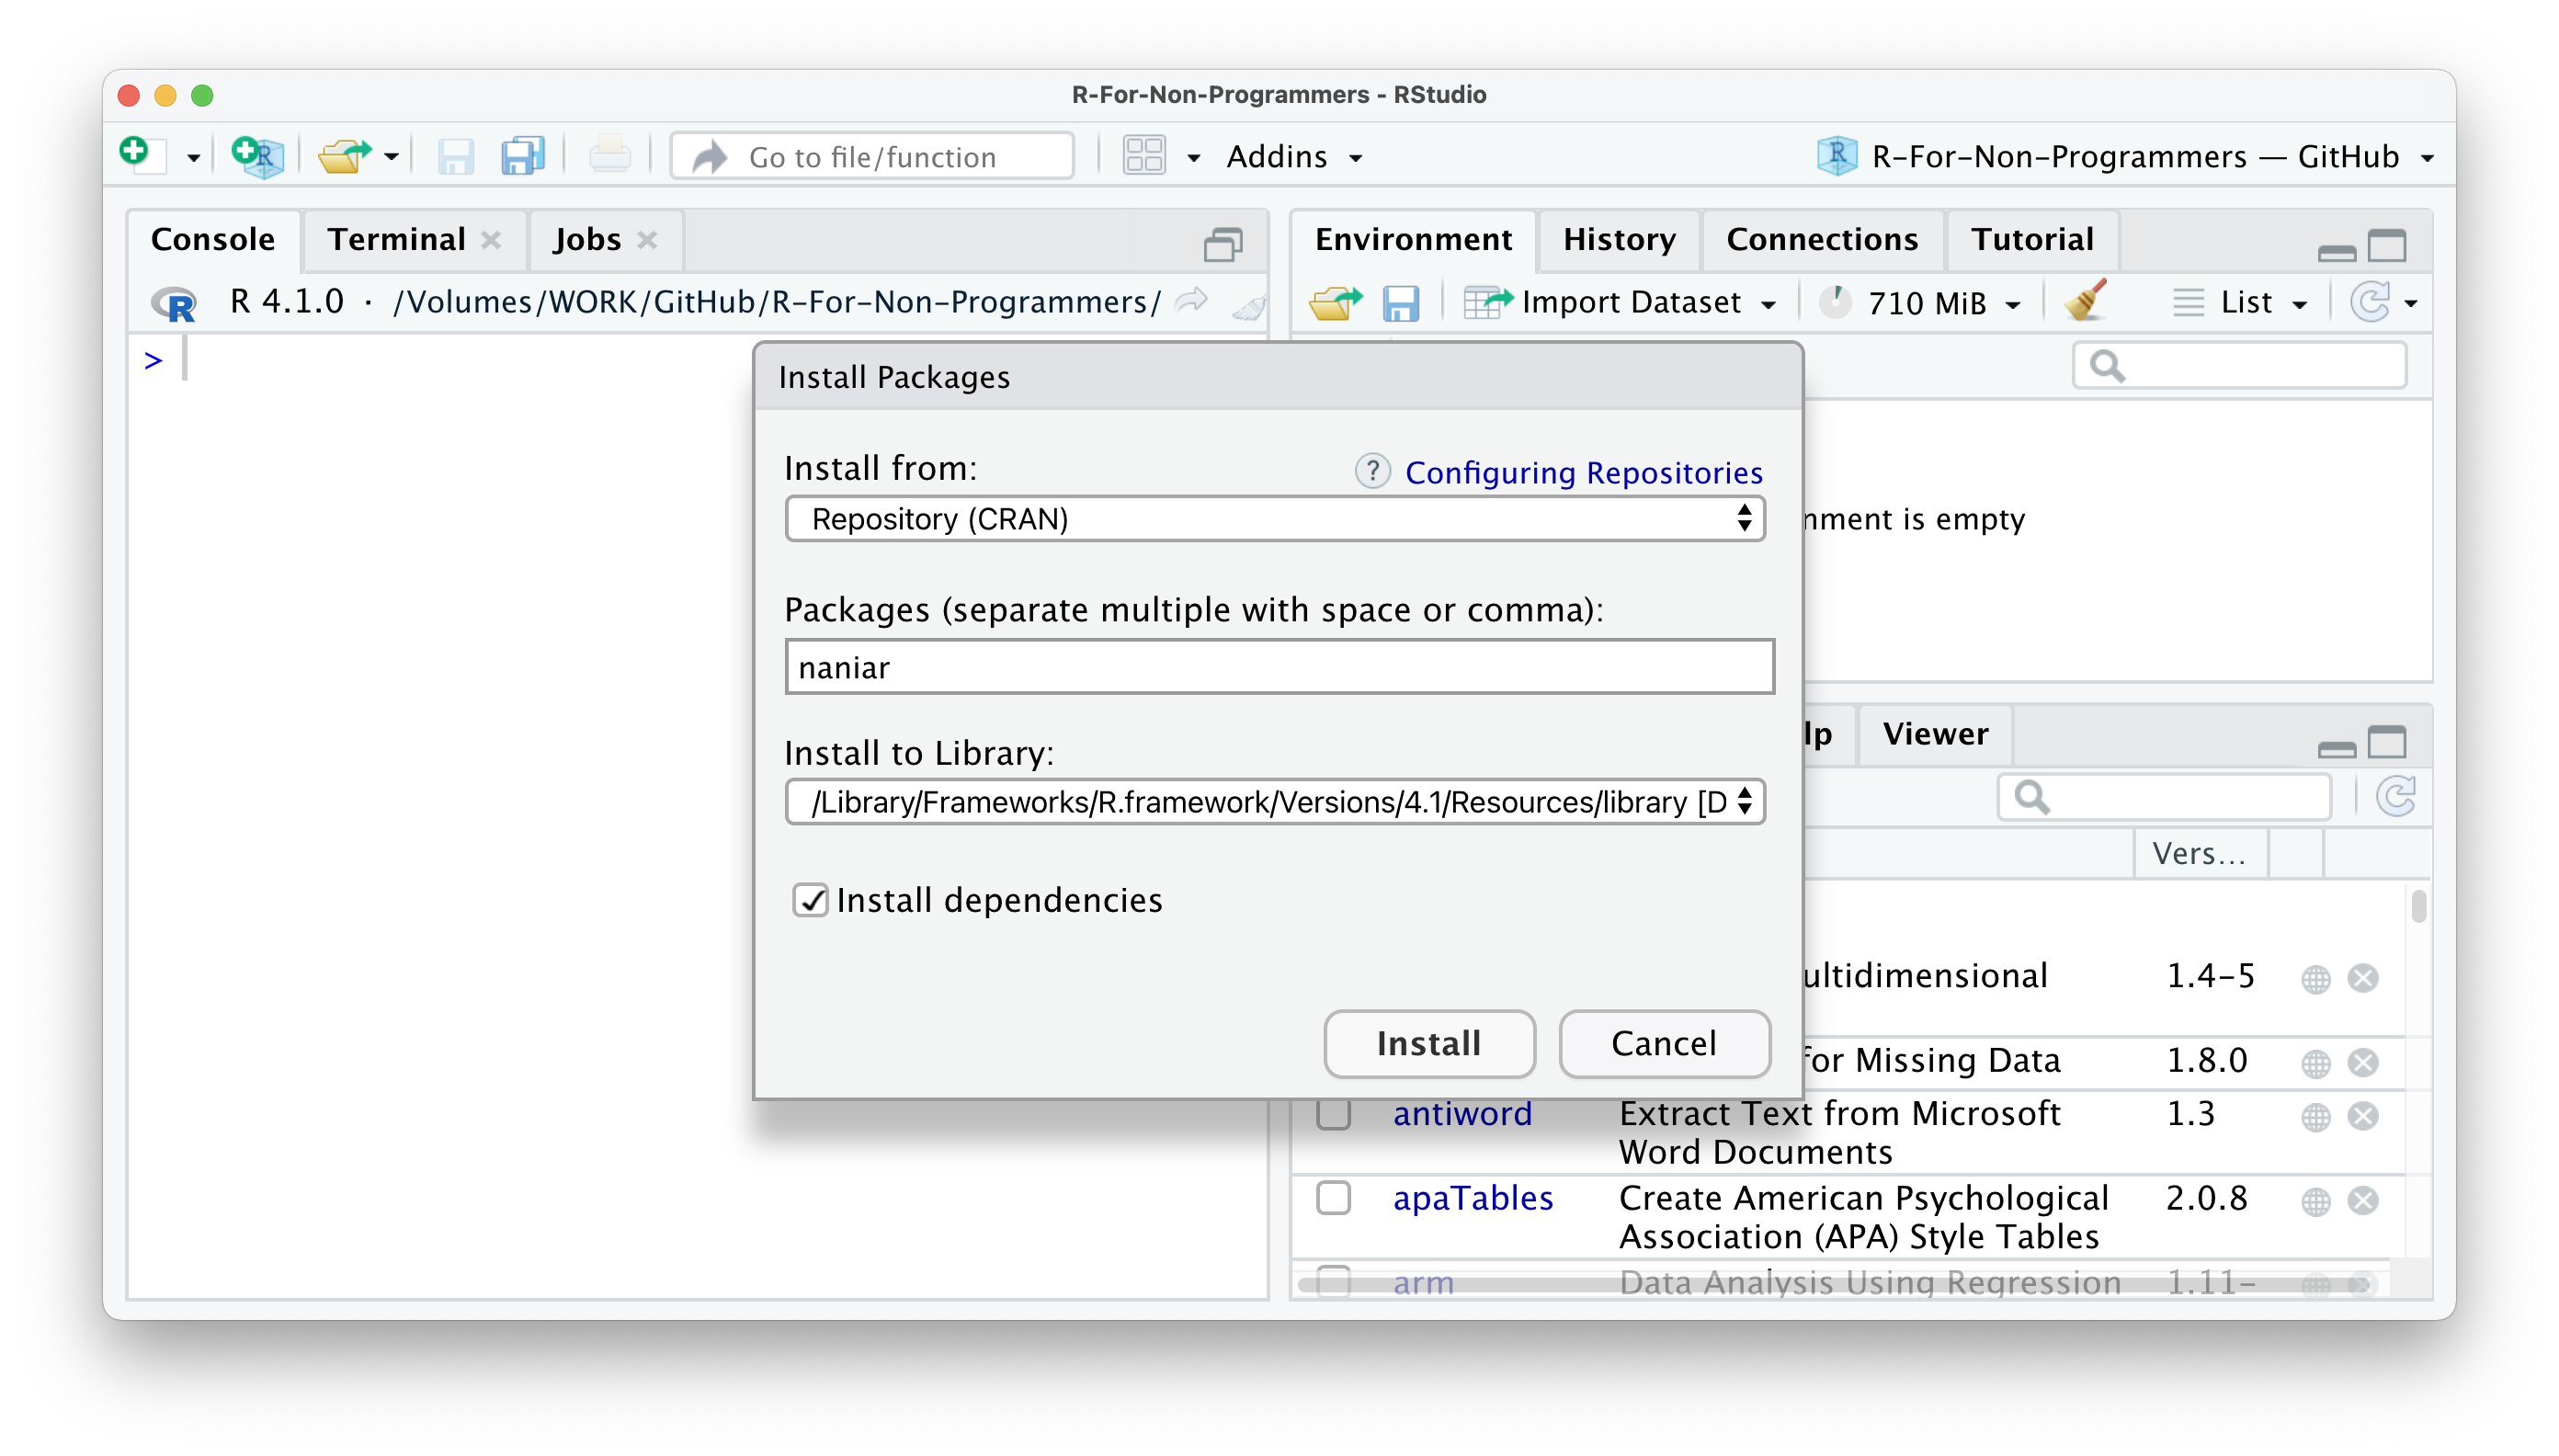
\includegraphics{images/chapter_05_img/install_r_packages/03_install_r_packages.png}
\end{enumerate}

The only real downside of using the packages pane is that you cannot
install packages hosted on GitHub only. However, you can download them
from there and install them directly from your computer using this
option. This is particularly useful if you do not have an internet
connection but you already downloaded the required packages onto a hard
drive. However, in 99.9\% of cases it is much easier to use the function
\texttt{devtools::install\_github()}.

\subsection{\texorpdfstring{Install all necessary \emph{R} packages for
this
book}{Install all necessary R packages for this book}}\label{install-all-r-packages}

Lastly, if you would like to install the necessary packages to follow
the examples in this book, the \texttt{r4np} package comes with a handy
function to install them all at once. Of course, you need to have
\texttt{r4np} installed first, as shown \hyperref[install-r4np]{above}.

\begin{Shaded}
\begin{Highlighting}[]
\CommentTok{\# Install all R packages used in this book}
\NormalTok{r4np}\SpecialCharTok{::}\FunctionTok{install\_r4np}\NormalTok{()}
\end{Highlighting}
\end{Shaded}

\subsection{\texorpdfstring{Using \emph{R}
Packages}{Using R Packages}}\label{using-r-packages}

Now that you have a nice collection of \emph{R} packages, the next step
would be to use them. While you only have to install \emph{R} packages
once, you have to `activate' them every time you start a new session in
RStudio. This process is also called `loading an \emph{R} package'. Once
an \emph{R} package is loaded, you can use all its functions. To load an
\emph{R} package, we have to use the function \texttt{library()}.

\begin{Shaded}
\begin{Highlighting}[]
\FunctionTok{library}\NormalTok{(tidyverse)}
\end{Highlighting}
\end{Shaded}

The \texttt{tidyverse} package is a special kind of package. It contains
multiple packages and loads them all at once. Almost all included
packages you will use at some point when working through this book.

I know what you are thinking. Can you use \texttt{c()} to load all your
packages at once? Unfortunately not. However, there is a way to do this,
but it goes beyond the scope of this book to fully explain this. If you
are curious, you can take a peek at the code
\href{https://stackoverflow.com/questions/8175912/load-multiple-packages-at-once}{here
on stackoverflow.com}.

Besides, it is not always advisable to load all functions of an entire
package. One reason could be that two packages contain a function with
the same name but with a different purpose. Two functions with the same
name create a conflict between these two packages, and one of the
functions would not be usable. Another reason could be that you only
need to use the function once, and loading the whole package to use only
one specific function seems excessive. Instead, you can explicitly call
functions from packages without loading the package. For example, we
might want to use the \texttt{vis\_miss()} function from the
\texttt{naniar} package to show where data is missing in our dataset
\texttt{airquality}. Using functions without \texttt{library()} is also
much quicker than loading the package and then calling the function if
you don't use it repeatedly. Make sure you have \texttt{naniar}
installed (see
\hyperref[install-packages-tidyverse-nanair-psych]{above}). We will work
with this package when we explore missing data in Chapter
@ref(dealing-with-missing-data). To use a function from an \emph{R}
package without loading it, we have to use \texttt{::} between the
package's name and the function we want to use. Copy the code below and
try it yourself.

\begin{Shaded}
\begin{Highlighting}[]
\CommentTok{\# Here I use the dataset \textquotesingle{}airquality\textquotesingle{}, which comes with R}
\NormalTok{naniar}\SpecialCharTok{::}\FunctionTok{vis\_miss}\NormalTok{(airquality)}
\end{Highlighting}
\end{Shaded}

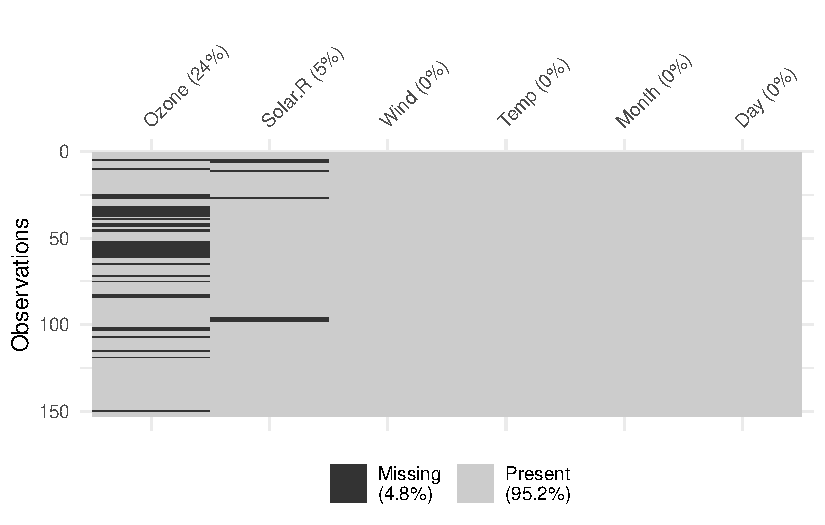
\includegraphics{05_r_basics_files/figure-pdf/explicitly-calling-functions-1.pdf}

\section{Coding etiquette}\label{coding-etiquette}

Now you know everything to get started, but before we jump into our
first project, I would like to briefly touch upon coding etiquette. This
is not something that improves your analytical or coding skills
directly, but is essential in building good habbits and making your life
and those of others a little easier. Consider writing code like growing
plants in your garden. You want to nurture the good plants, remove the
weed and add labels that tell you which plant it is that you are
growing. At the end of the day, you want your garden to be
well-maintained. Treat you programming code the same way.

A script (see Chapter @ref(creating-an-r-script)) of programming code
should always have at least the following qualities:

\begin{itemize}
\item
  Only contains code that is necessary,
\item
  Is easy to read and understand,
\item
  Is self-contained.
\end{itemize}

With simple code this is easily achieved. However, what about more
complex and longer code representing a whole set of analytical steps?

\begin{Shaded}
\begin{Highlighting}[]
\CommentTok{\# Very messy code}

\FunctionTok{library}\NormalTok{(tidyverse)}
\FunctionTok{library}\NormalTok{(jtools)}
\NormalTok{model1 }\OtherTok{\textless{}{-}} \FunctionTok{lm}\NormalTok{(covid\_cases\_per\_1m }\SpecialCharTok{\textasciitilde{}}\NormalTok{ idv, }\AttributeTok{data =}\NormalTok{ df)}
\FunctionTok{summ}\NormalTok{(model1, }\AttributeTok{scale =} \ConstantTok{TRUE}\NormalTok{, }\AttributeTok{transform.response =} \ConstantTok{TRUE}\NormalTok{, }\AttributeTok{vifs =} \ConstantTok{TRUE}\NormalTok{)}
\NormalTok{df }\SpecialCharTok{\%\textgreater{}\%} \FunctionTok{ggplot}\NormalTok{(}\FunctionTok{aes}\NormalTok{(}\AttributeTok{x =}\NormalTok{ covid\_cases\_per\_1m, }\AttributeTok{y =}\NormalTok{ idv, }\AttributeTok{col =}\NormalTok{ europe, }\AttributeTok{label =}\NormalTok{ country))}\SpecialCharTok{+}
\FunctionTok{theme\_minimal}\NormalTok{()}\SpecialCharTok{+} \FunctionTok{geom\_label}\NormalTok{(}\AttributeTok{nudge\_y =} \DecValTok{2}\NormalTok{) }\SpecialCharTok{+} \FunctionTok{geom\_point}\NormalTok{()}
\NormalTok{model2 }\OtherTok{\textless{}{-}} \FunctionTok{lm}\NormalTok{(cases\_per\_1m }\SpecialCharTok{\textasciitilde{}}\NormalTok{ idv }\SpecialCharTok{+}\NormalTok{ uai }\SpecialCharTok{+}\NormalTok{ idv}\SpecialCharTok{*}\NormalTok{europe }\SpecialCharTok{+}\NormalTok{ uai}\SpecialCharTok{*}\NormalTok{europe, }\AttributeTok{data =}\NormalTok{ df)}
\FunctionTok{summ}\NormalTok{(model2, }\AttributeTok{scale =} \ConstantTok{TRUE}\NormalTok{, }\AttributeTok{transform.response =} \ConstantTok{TRUE}\NormalTok{, }\AttributeTok{vifs =} \ConstantTok{TRUE}\NormalTok{)}
\FunctionTok{anova}\NormalTok{(model1, model2)}
\end{Highlighting}
\end{Shaded}

How about the following in comparison?

\begin{Shaded}
\begin{Highlighting}[]
\CommentTok{\# Nicely structured code}

\CommentTok{\# Load required R packages}
\FunctionTok{library}\NormalTok{(tidyverse)}
\FunctionTok{library}\NormalTok{(jtools)}

\CommentTok{\# {-}{-}{-}{-} Modelling COVID{-}19 cases {-}{-}{-}{-}}

\DocumentationTok{\#\# Specify and run a regression}
\NormalTok{model1 }\OtherTok{\textless{}{-}} \FunctionTok{lm}\NormalTok{(covid\_cases\_per\_1m }\SpecialCharTok{\textasciitilde{}}\NormalTok{ idv, }\AttributeTok{data =}\NormalTok{ df)}

\DocumentationTok{\#\# Retrieve the summary statistics of model1}
\FunctionTok{summ}\NormalTok{(model1,}
     \AttributeTok{scale =} \ConstantTok{TRUE}\NormalTok{,}
     \AttributeTok{transform.response =} \ConstantTok{TRUE}\NormalTok{,}
     \AttributeTok{vifs =} \ConstantTok{TRUE}\NormalTok{)}

\CommentTok{\# Does is matter whether a country lies in Europe?}

\DocumentationTok{\#\# Visualise rel. of covid cases, idv and being a European country}
\NormalTok{df }\SpecialCharTok{\%\textgreater{}\%}
  \FunctionTok{ggplot}\NormalTok{(}\FunctionTok{aes}\NormalTok{(}\AttributeTok{x =}\NormalTok{ covid\_cases\_per\_1m,}
             \AttributeTok{y =}\NormalTok{ idv,}
             \AttributeTok{col =}\NormalTok{ europe,}
             \AttributeTok{label =}\NormalTok{ country)) }\SpecialCharTok{+}
  \FunctionTok{theme\_minimal}\NormalTok{() }\SpecialCharTok{+}
  \FunctionTok{geom\_label}\NormalTok{(}\AttributeTok{nudge\_y =} \DecValTok{2}\NormalTok{) }\SpecialCharTok{+}
  \FunctionTok{geom\_point}\NormalTok{()}

\DocumentationTok{\#\# Specify and run a revised regression}
\NormalTok{model2 }\OtherTok{\textless{}{-}} \FunctionTok{lm}\NormalTok{(cases\_per\_1m }\SpecialCharTok{\textasciitilde{}}\NormalTok{ idv }\SpecialCharTok{+}\NormalTok{ uai }\SpecialCharTok{+}\NormalTok{ idv}\SpecialCharTok{*}\NormalTok{europe }\SpecialCharTok{+}\NormalTok{ uai}\SpecialCharTok{*}\NormalTok{europe,}
                 \AttributeTok{data =}\NormalTok{ df)}

\DocumentationTok{\#\# Retrieve the summary statistics of model2}
\FunctionTok{summ}\NormalTok{(model2,}
     \AttributeTok{scale =} \ConstantTok{TRUE}\NormalTok{,}
     \AttributeTok{transform.response =} \ConstantTok{TRUE}\NormalTok{,}
     \AttributeTok{vifs =} \ConstantTok{TRUE}\NormalTok{)}

\DocumentationTok{\#\# Test whether model2 is an improvement over model1}
\FunctionTok{anova}\NormalTok{(model1, model2)}
\end{Highlighting}
\end{Shaded}

I hope we can agree that the second example is much easier to read and
understand even though you probably do not understand most of it yet.
For once, I separated the different analytical steps from each other
like paragraphs in a report. Apart from that, I added comments with
\texttt{\#} to provide more context to my code for someone else who
wants to understand my analysis. Admittedly, this example is a little
excessive. Usually, you might have fewer comments. Commenting is an
integral part of programming because it allows you to remember what you
did. Ideally, you want to strike a good balance between commenting on
and writing your code. How many comments you need will likely change
throughout your \emph{R} programming journey. Think of comments as
headers for your programming script that give it structure.

We can use \texttt{\#} not only to write comments but also to tell R not
to run particular code. This is very helpful if you want to keep some
code but do not want to use it yet. There is also a handy keyboard
shortcut you can use to `deactivate' multiple lines of code at once.
Select whatever you want to `comment out' in your script and press
\texttt{Ctrl+Shift+C} (PC) or \texttt{Cmd+Shift+C} (Mac).

\begin{Shaded}
\begin{Highlighting}[]
\CommentTok{\# mean(pocket\_money) \# R will NOT run this code}
\FunctionTok{mean}\NormalTok{(pocket\_money)   }\CommentTok{\# R will run this code}
\end{Highlighting}
\end{Shaded}

RStudio helps a lot with keeping your coding tidy and properly
formatted. However, there are some additional aspects worth considering.
If you want to find out more about coding style, I highly recommend to
read through \href{https://style.tidyverse.org}{\emph{`The tidyverse
style guide'}} (Wickham 2021).\\

\section{Exercises}\label{exercises-r_basics}

It is time to practice the newly acquired skills. The \texttt{r4np}
package comes with interactive tutorials. In order to start them, you
have two options. If you have installed the \texttt{r4np} package
already and used the function \texttt{install\_r4np()} you can use
\texttt{Option\ 1}:

\begin{Shaded}
\begin{Highlighting}[]
\CommentTok{\# Option 1:}
\NormalTok{learnr}\SpecialCharTok{::}\FunctionTok{run\_tutorial}\NormalTok{(}\StringTok{"ex\_r\_basics"}\NormalTok{, }\AttributeTok{package =} \StringTok{"r4np"}\NormalTok{)}
\end{Highlighting}
\end{Shaded}

If you have not installed the \texttt{r4np} package and/or not run the
function \texttt{install\_r4np()}, you will have to do this first using
\texttt{Option\ 2}:

\begin{Shaded}
\begin{Highlighting}[]
\CommentTok{\# Option 2:}
\DocumentationTok{\#\# Install \textquotesingle{}r4np\textquotesingle{} package}
\NormalTok{devtools}\SpecialCharTok{::}\FunctionTok{install\_github}\NormalTok{(}\StringTok{"ddauber/r4np"}\NormalTok{)}

\DocumentationTok{\#\# Install all relevant packages for this book}
\NormalTok{r4np}\SpecialCharTok{::}\FunctionTok{install\_r4np}\NormalTok{()}

\DocumentationTok{\#\# Start the tutorial for this chapter}
\NormalTok{learnr}\SpecialCharTok{::}\FunctionTok{run\_tutorial}\NormalTok{(}\StringTok{"ex\_r\_basics"}\NormalTok{, }\AttributeTok{package =} \StringTok{"r4np"}\NormalTok{)}
\end{Highlighting}
\end{Shaded}

\bookmarksetup{startatroot}

\chapter{\texorpdfstring{Starting your \emph{R}
projects}{Starting your R projects}}\label{starting-your-r-projects}

Every new project likely fills you with enthusiasm and excitement. And
it should. You are about to find answers to your research questions, and
you hopefully come out more knowledgeable due to it. However, there are
likely certain aspects of data analysis that you find less enjoyable. I
can think of two:

\begin{itemize}
\item
  Keeping track of all the files my project generates
\item
  Data wrangling
\end{itemize}

While we cover data wrangling in great detail in the next Chapter
(Chapter @ref(data-wrangling)), I would like to share some insights from
my work that helped me stay organised and, consequently, less
frustrated. The following applies to small and large research projects,
which makes it very convenient no matter the situation and the scale of
the project. Of course, feel free to tweak my approach to whatever suits
you. However, consistency is king.

\section{\texorpdfstring{Creating an \emph{R} Project
file}{Creating an R Project file}}\label{creating-an-r-project}

When working on a project, you likely create many different files for
various purposes, especially \emph{R} Scripts (see Chapter
@ref(creating-an-r-script)). If you are not careful, this file is stored
in your system's default location, which might not be where you want
them to be. RStudio allows you to manage your entire project intuitively
and conveniently through \emph{R} Project files. Using \emph{R} Project
files comes with a couple of perks, for example:

\begin{itemize}
\item
  All the files that you generate are in the same place. Your data, your
  coding, your exported plots, your reports, etc., all are in one place
  together without you having to manage the files manually. This is due
  to the fact that RStudio sets the root directory to whichever folder
  your project is saved to.
\item
  If you want to share your project, you can share the entire folder,
  and others can quickly reproduce your research or help fix problems.
  This is because all file paths are relative and not absolute.
\item
  You can, more easily, use GitHub for backups and so-called `version
  control', which allows you to track changes you have made to your code
  over time (see also Chapter @ref(next-steps-github)).
\end{itemize}

For now, the most important reason to use \emph{R} Project files is the
convenience of the organisation of files and the ability to share it
easily with co-investigators, your supervisor, or your students.

To create an R Project, you need to perform the following steps:

\begin{enumerate}
\def\labelenumi{\arabic{enumi}.}
\item
  Select \texttt{File\ \textgreater{}\ New\ Project…} from the menu bar.

  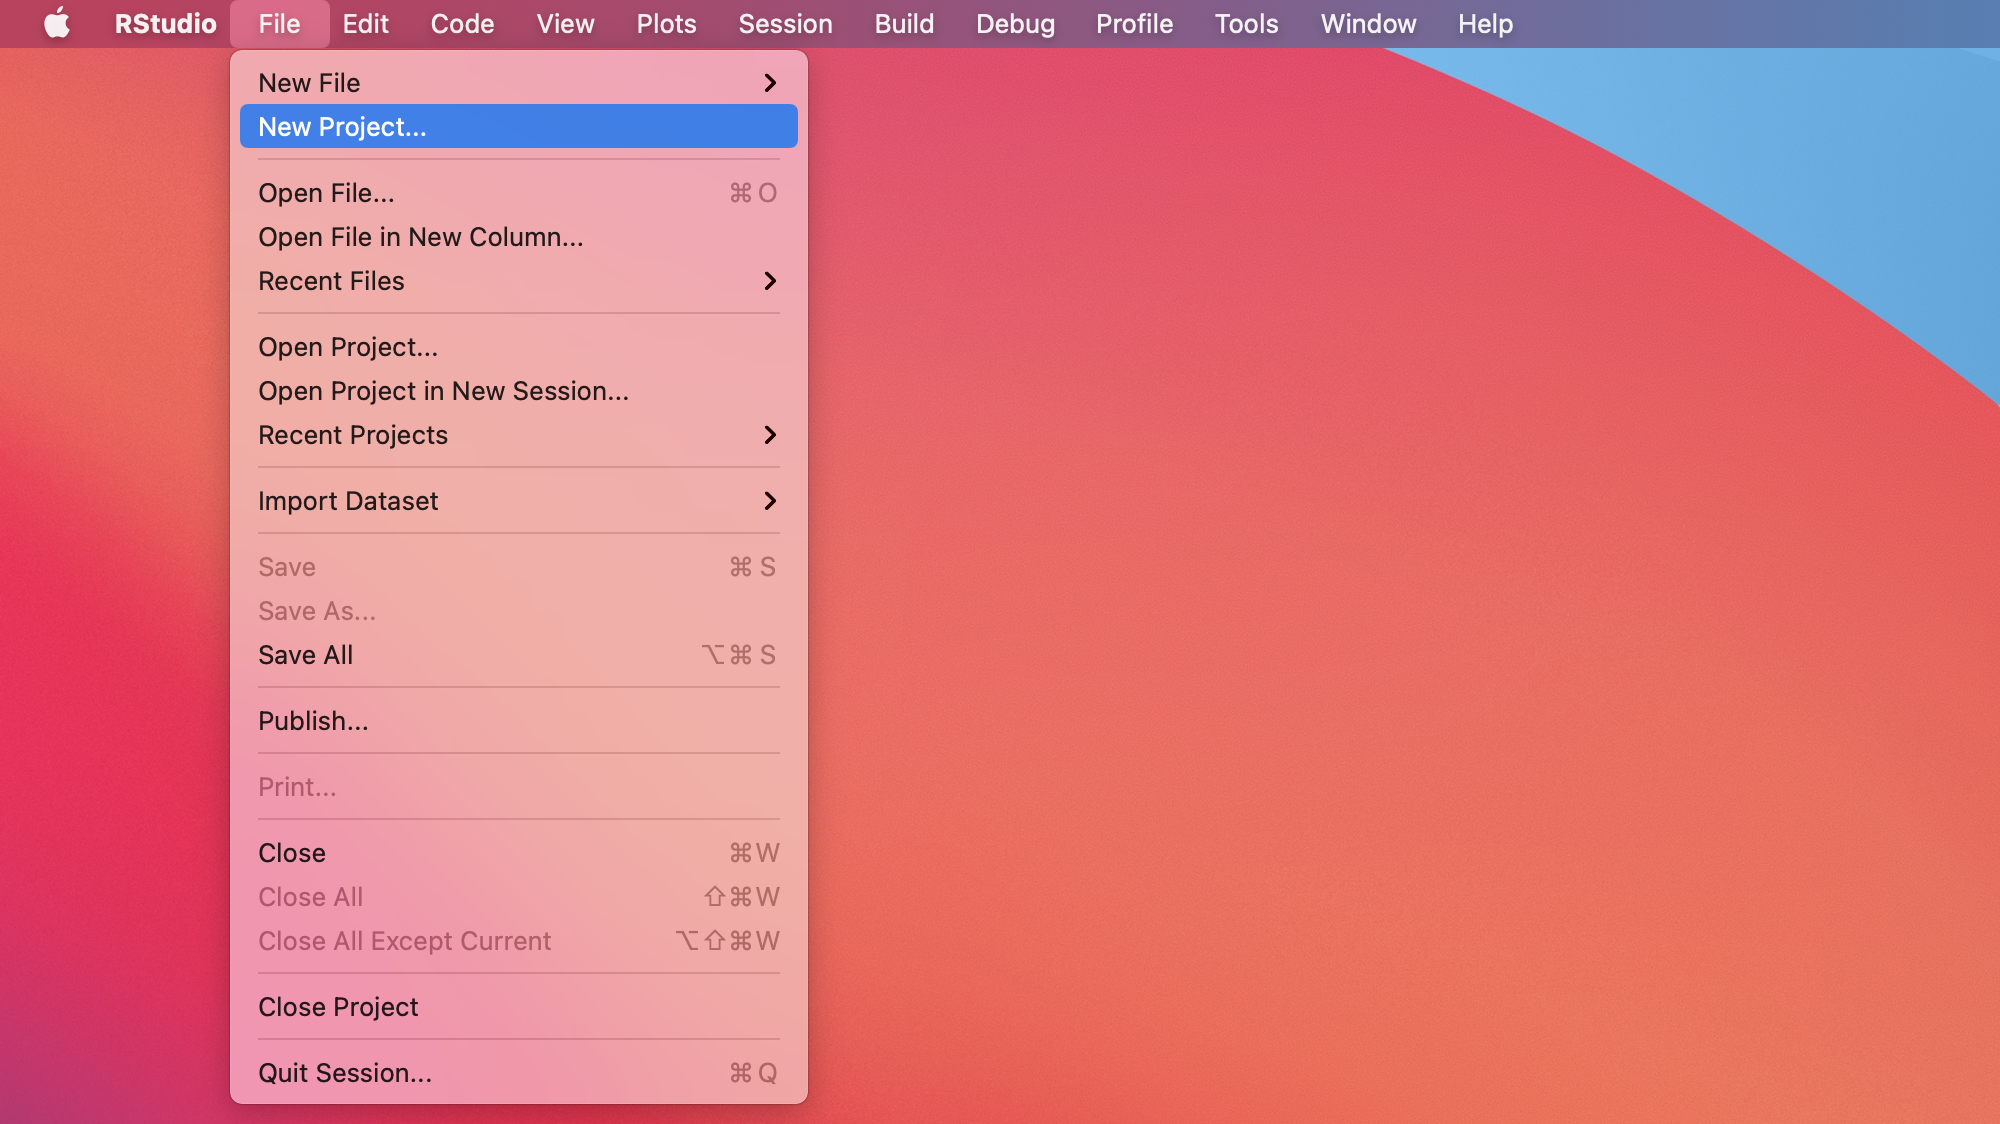
\includegraphics{images/chapter_06_img/00_r_project/00_r_project_file_menu.png}
\item
  Select \texttt{New\ Directory} from the popup window.

  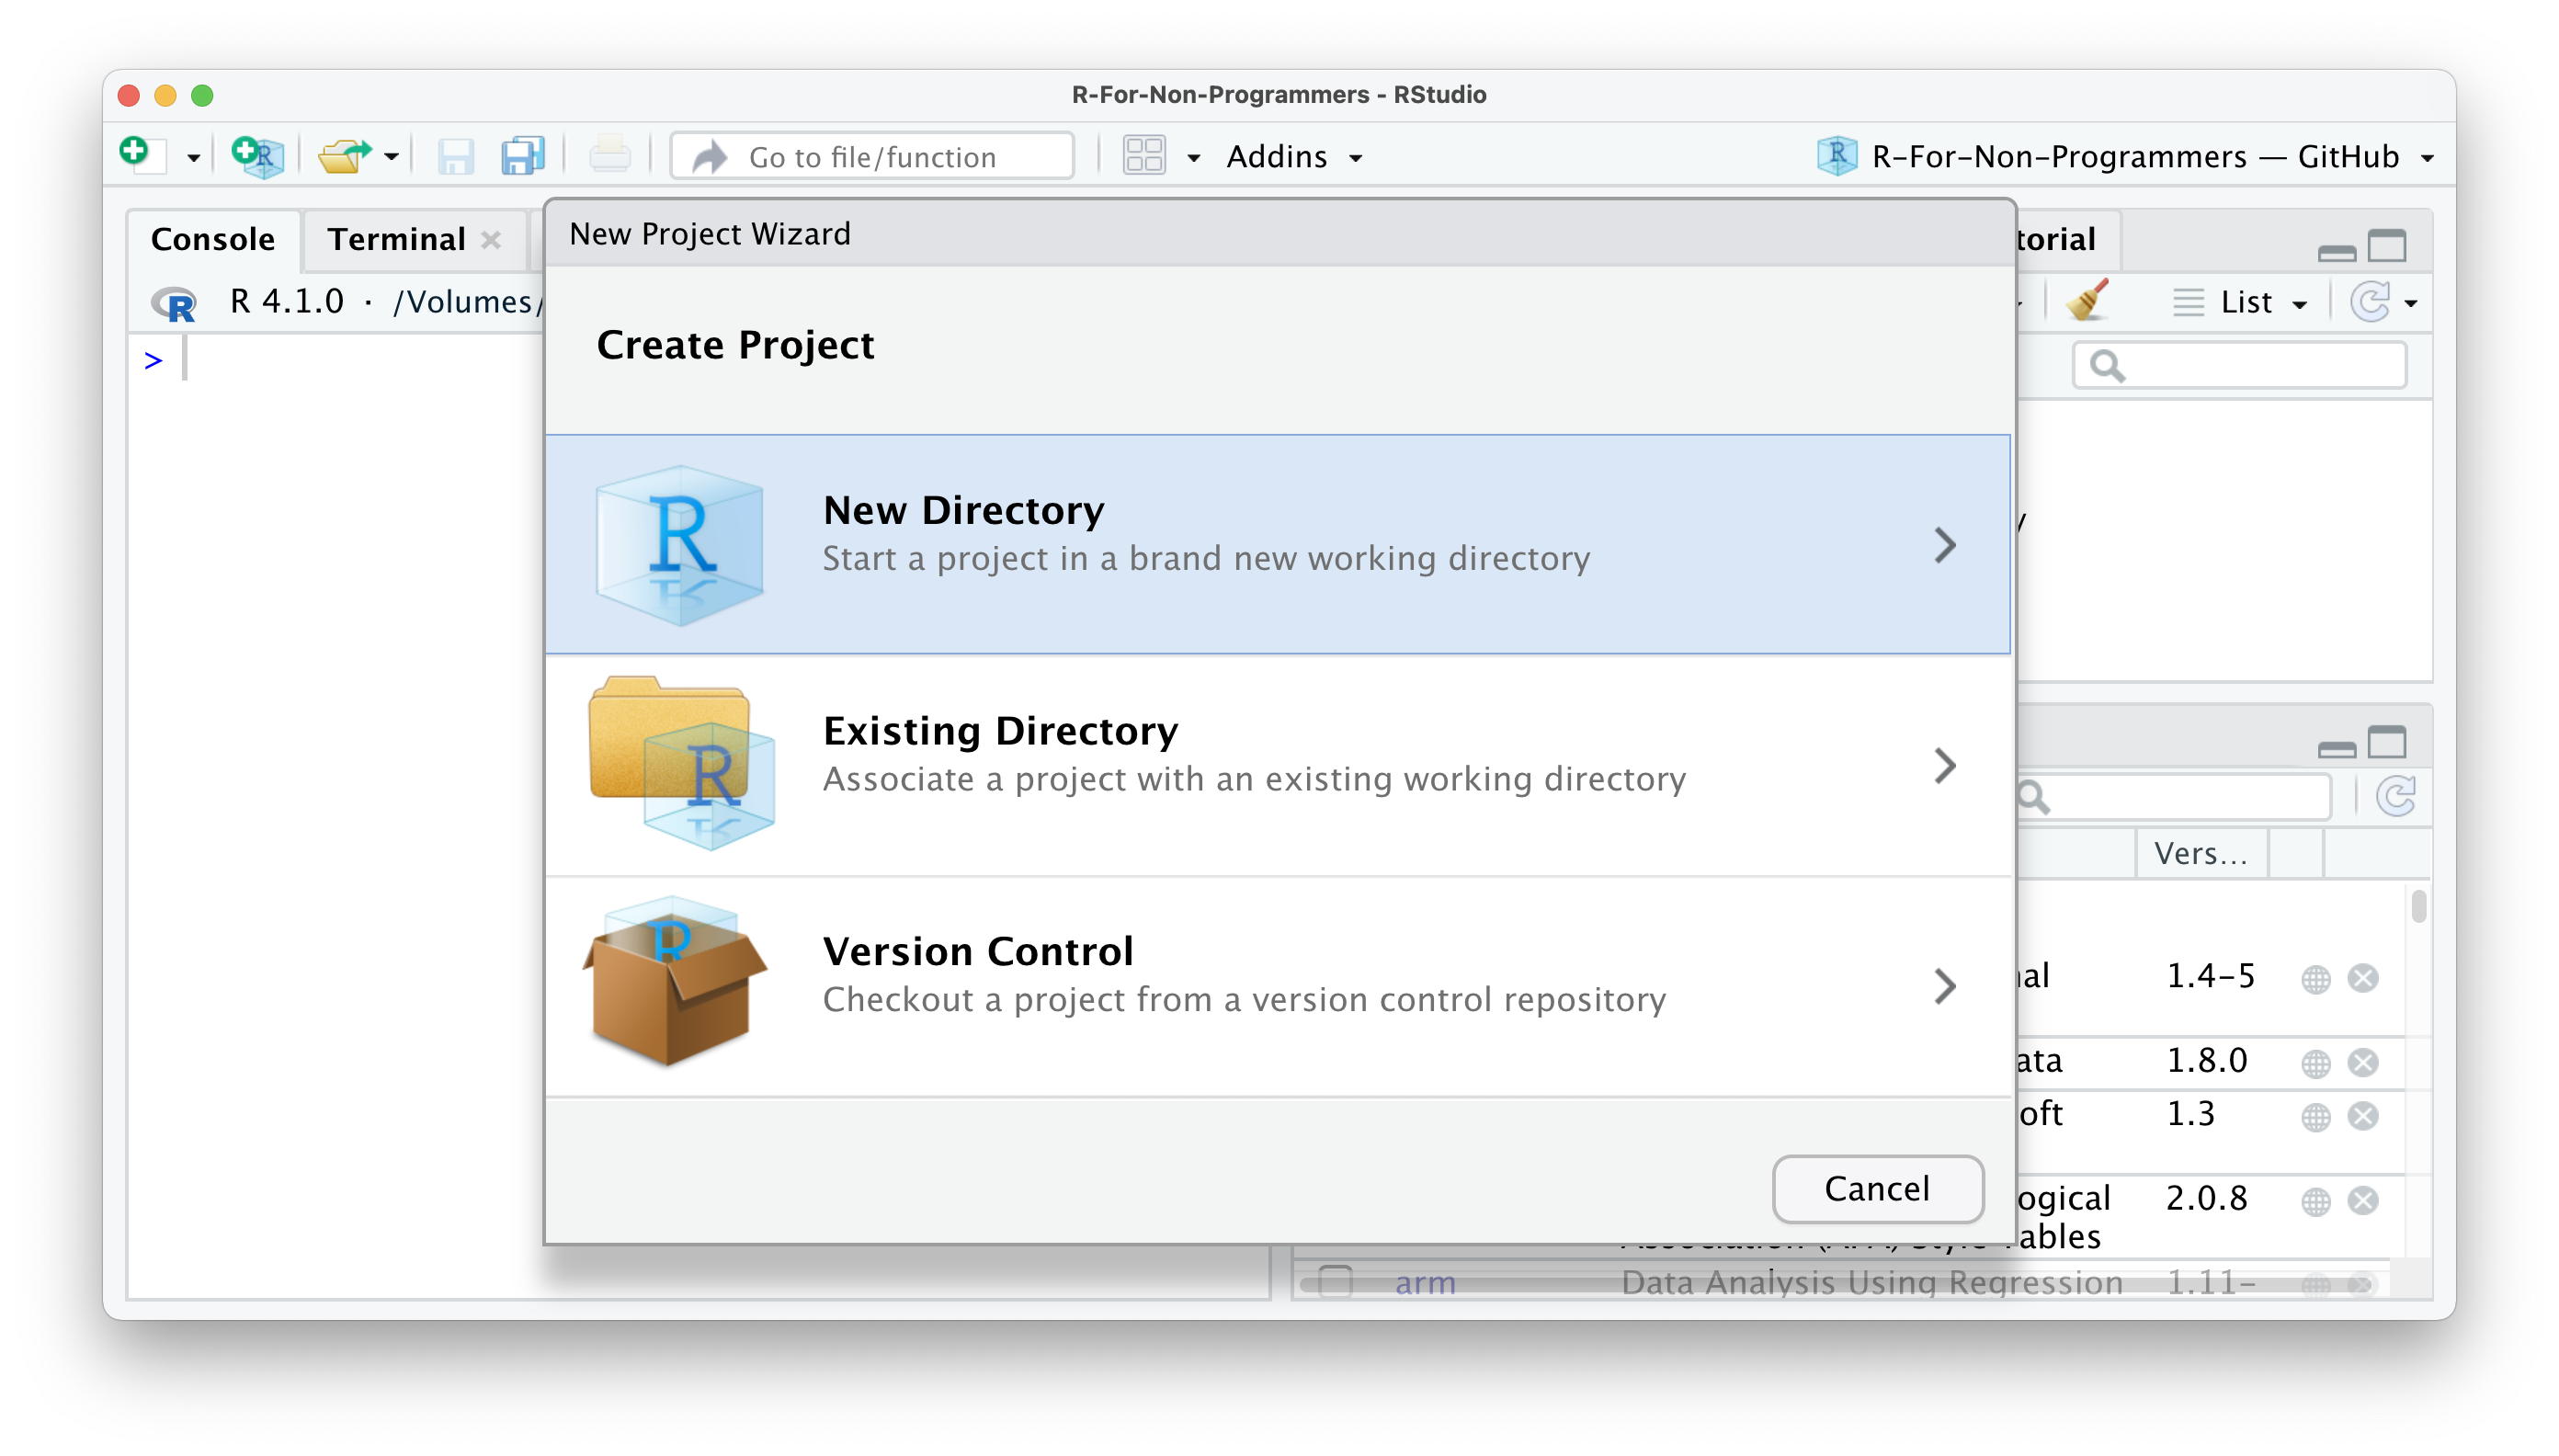
\includegraphics{images/chapter_06_img/00_r_project/01_r_project_new_directory.png}
\item
  Next, select \texttt{New\ Project}.

  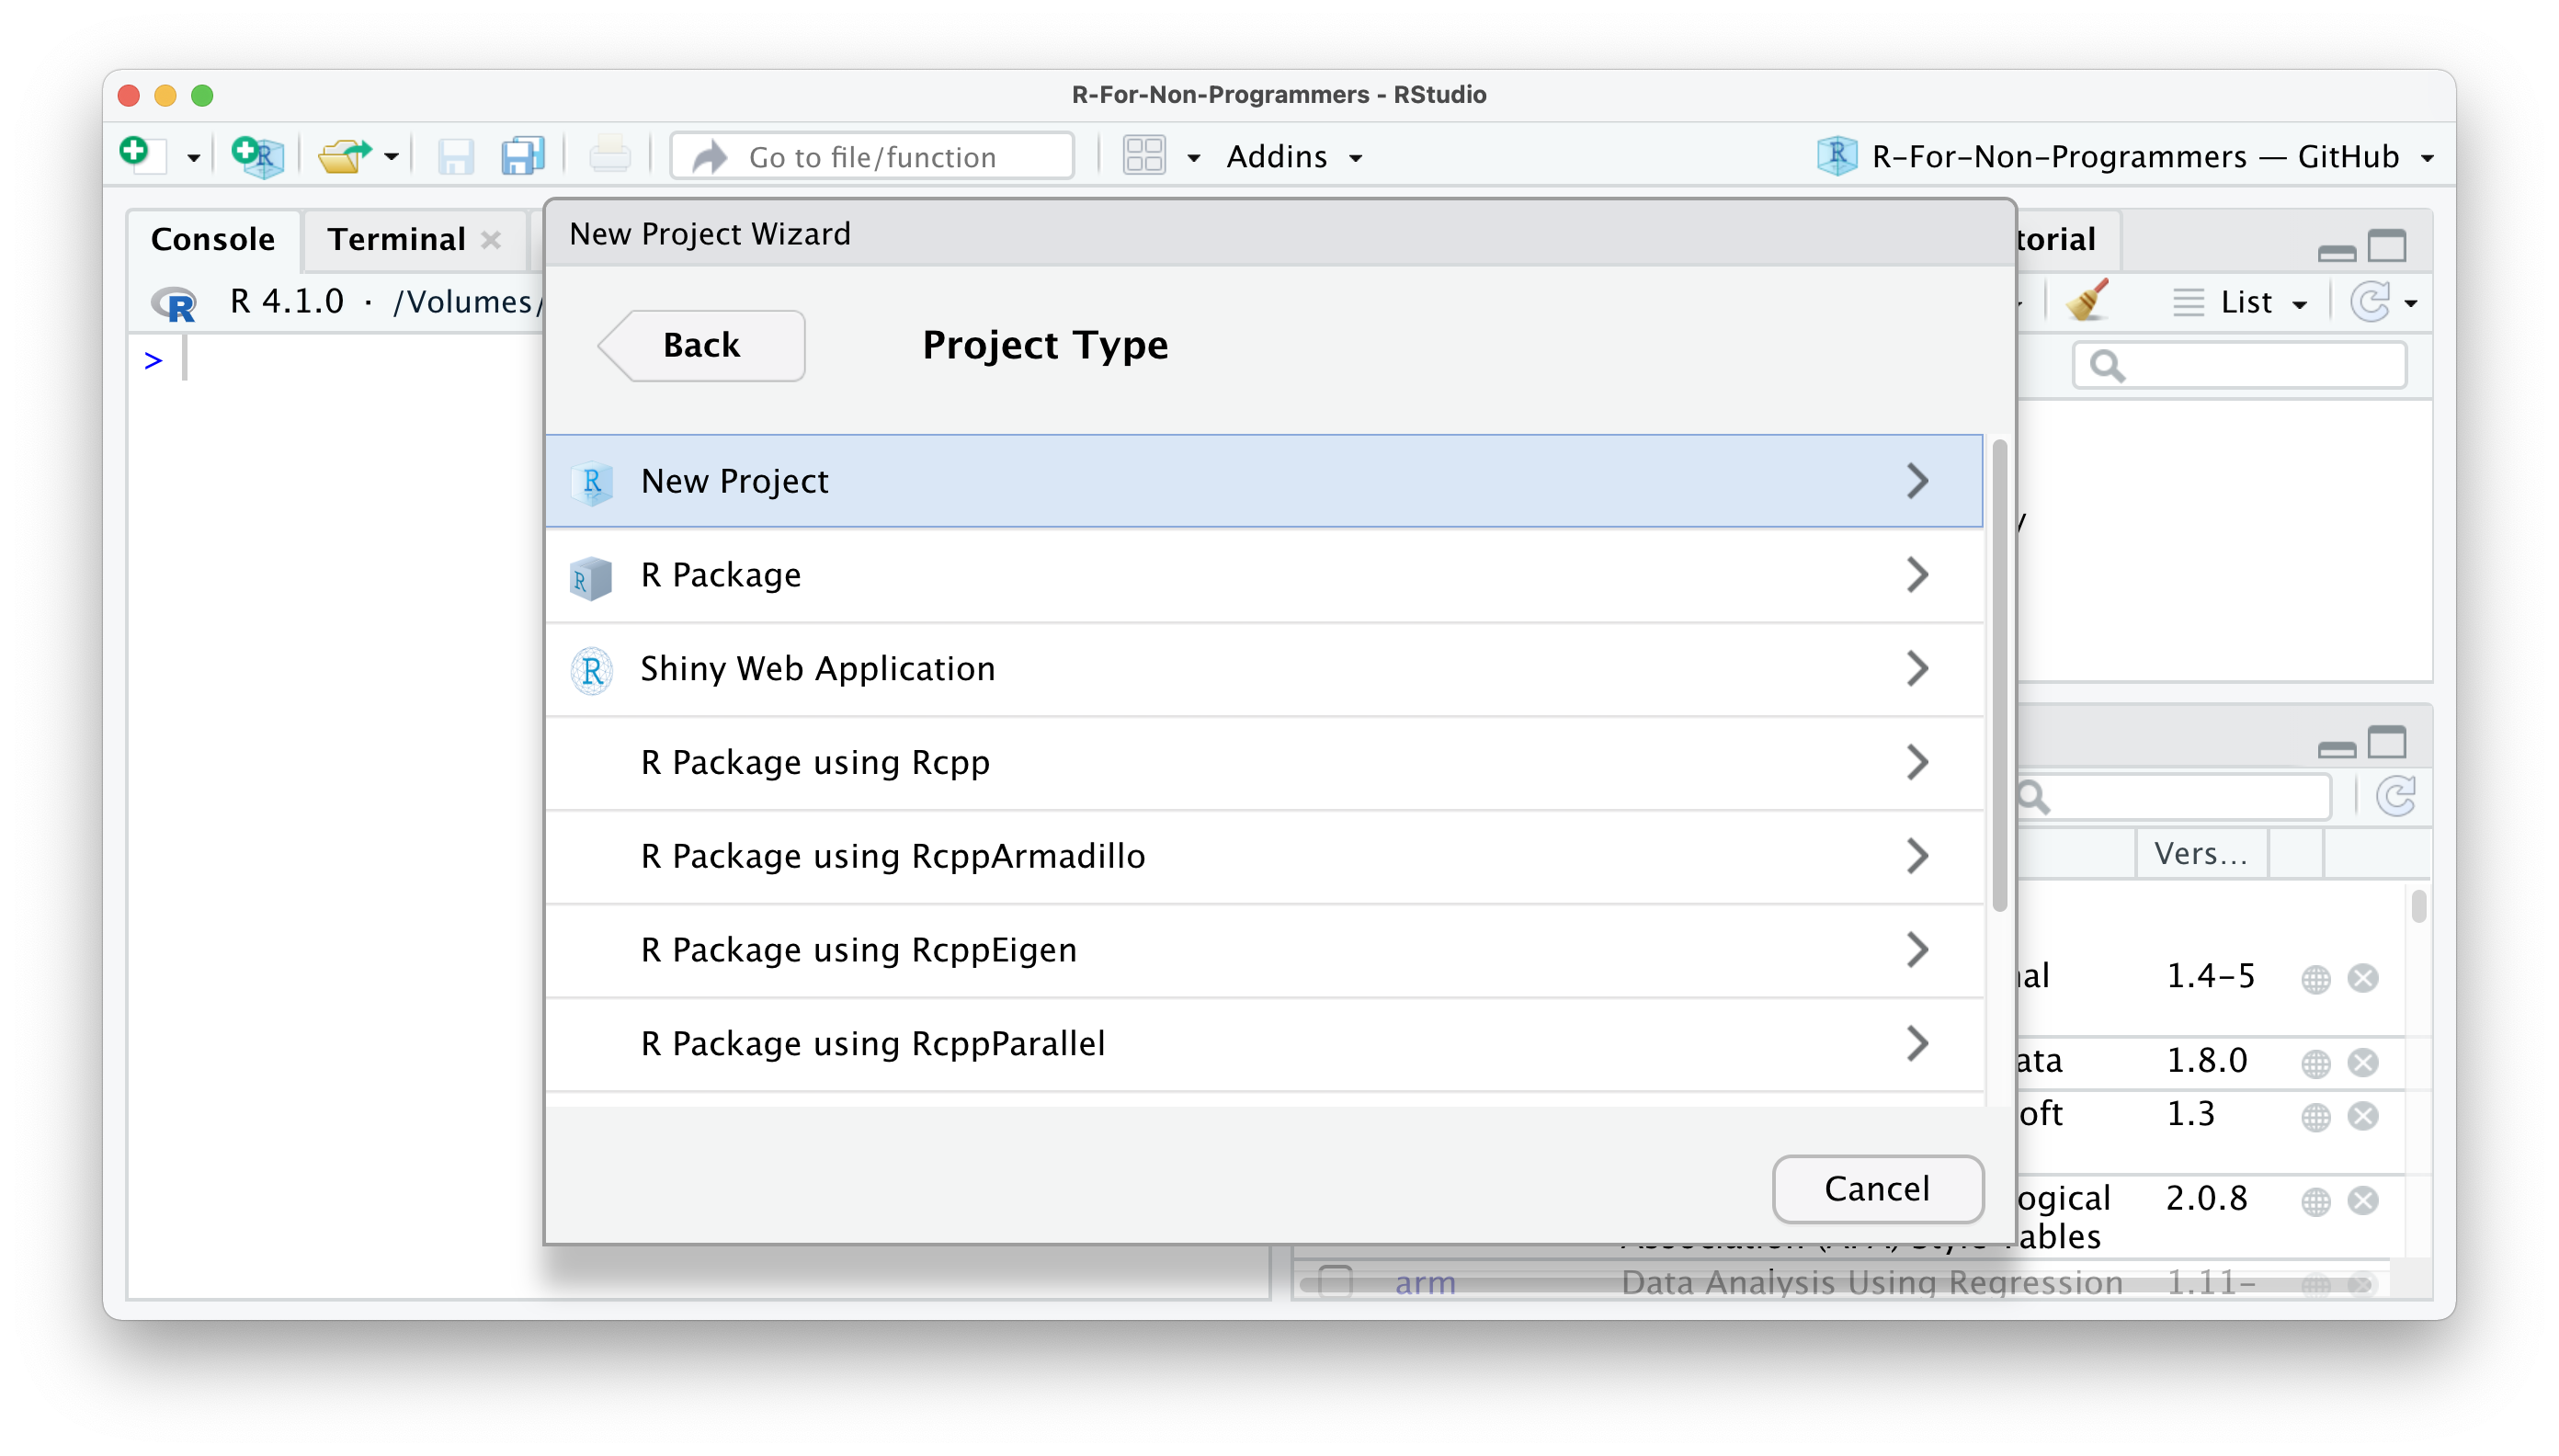
\includegraphics{images/chapter_06_img/00_r_project/02_r_project_new_project.png}
\item
  Pick a meaningful name for your project folder, i.e.~the
  \texttt{Directory\ Name}. Ensure this project folder is created in the
  right place. You can change the \texttt{subdirectory} by clicking on
  \texttt{Browse…}. Ideally the subdirectory is a place where you
  usually store your research projects.

  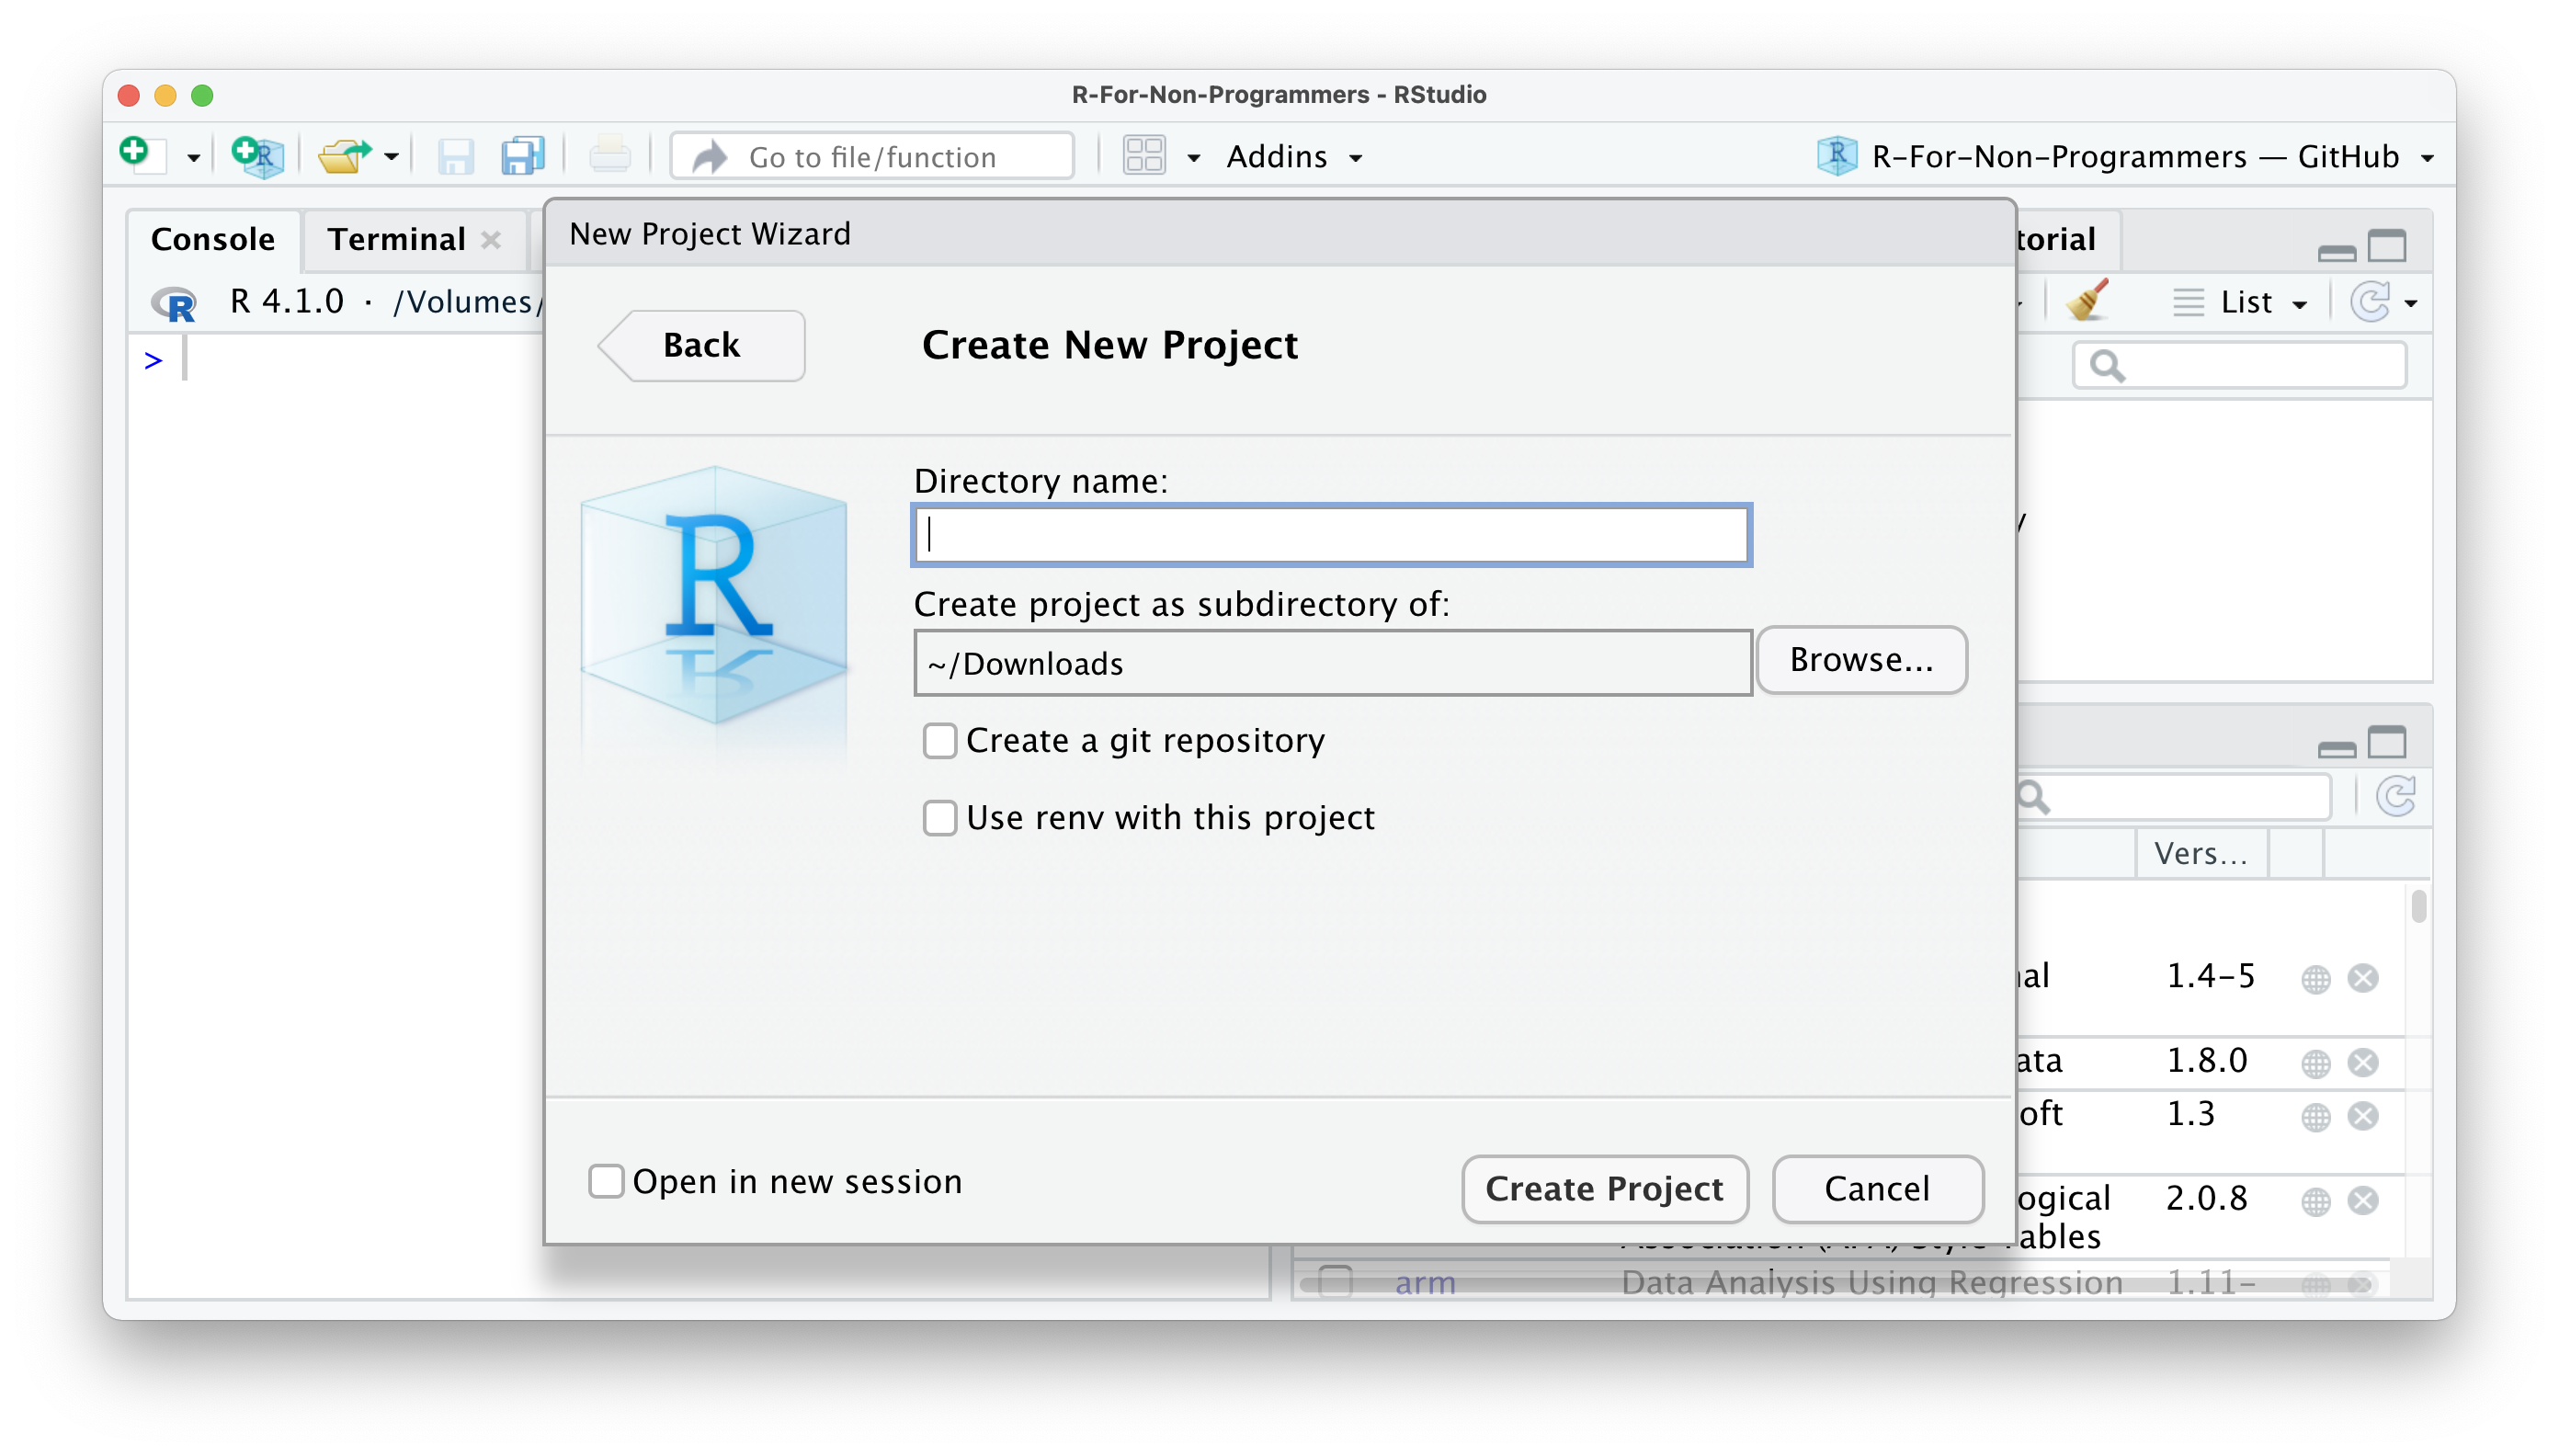
\includegraphics{images/chapter_06_img/00_r_project/03_r_project_specs.png}
\item
  You have the option to \texttt{Create\ a\ git\ repository}. This is
  only relevant if you already have a GitHub account and wish to use
  version control. For now, you can happily ignore it if you do not use
  GitHub.
\item
  Lastly, tick \texttt{Open\ in\ new\ session}. This will open your
  \emph{R} Project in a new RStudio window.

  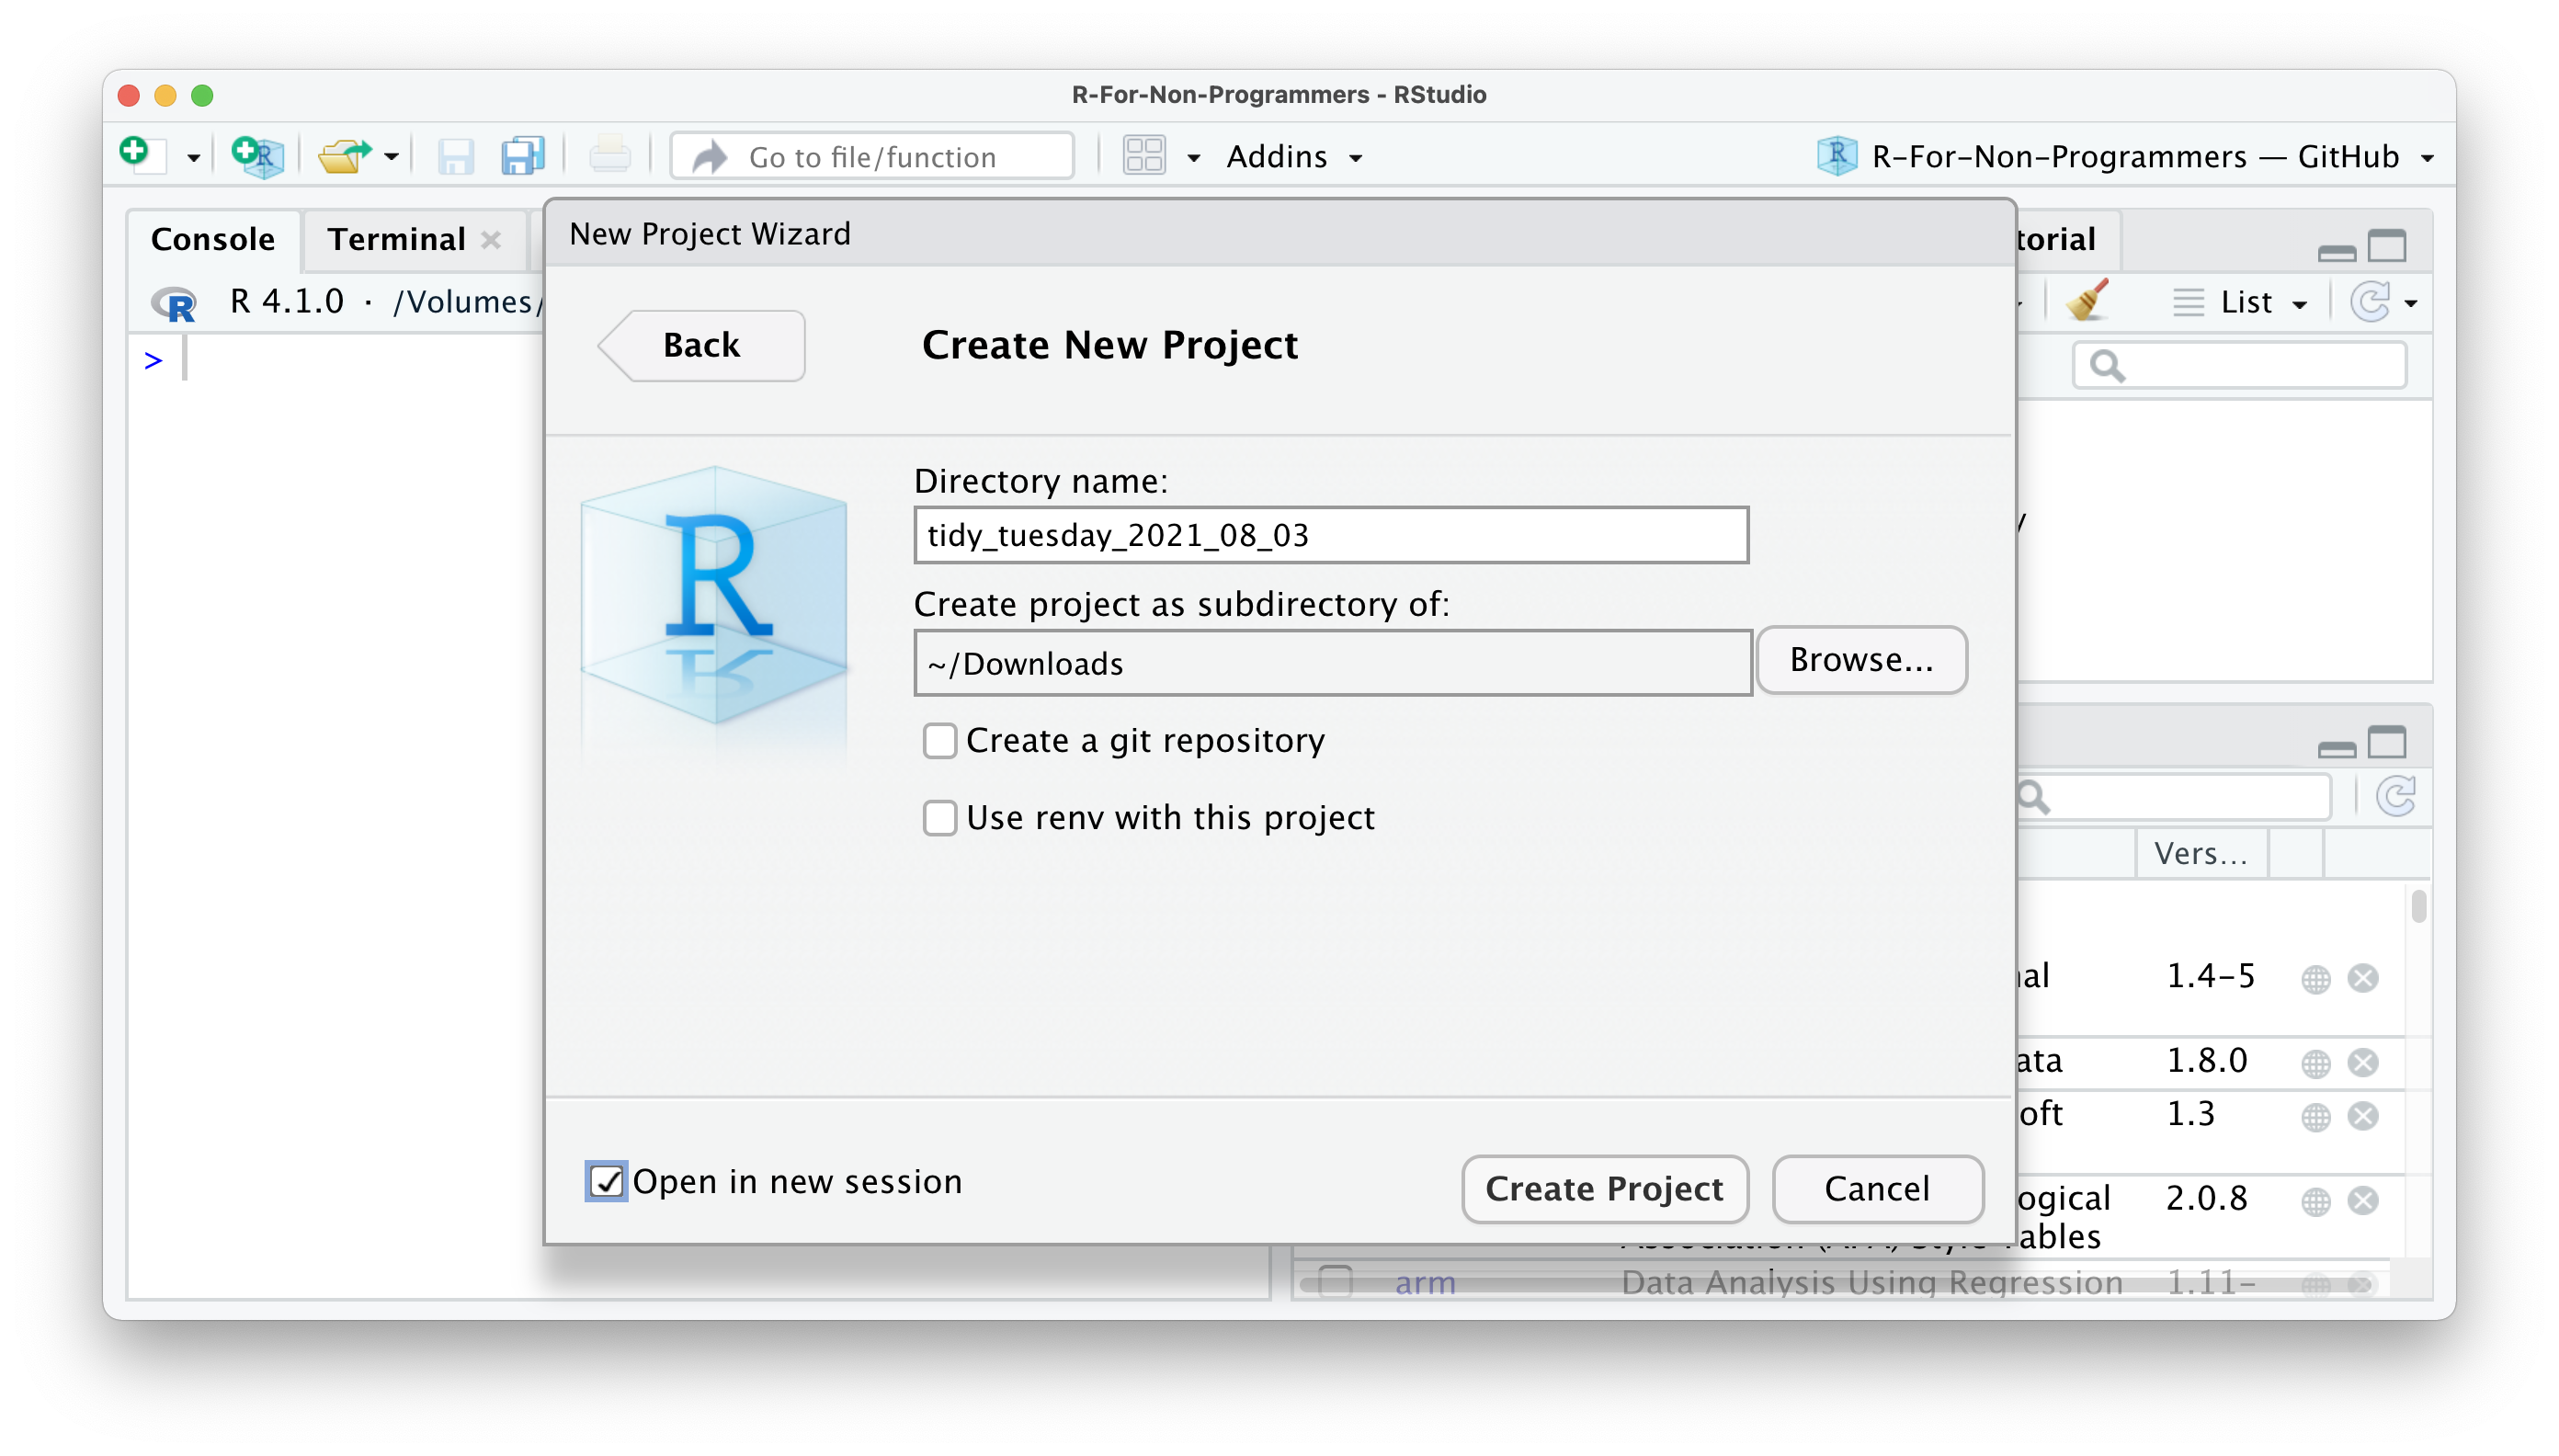
\includegraphics{images/chapter_06_img/00_r_project/04_r_project_directory_name.png}
\item
  Once you are happy with your choices, you can click
  \texttt{Create\ Project}. This will open a new \emph{R} Session, and
  you can start working on your project.

  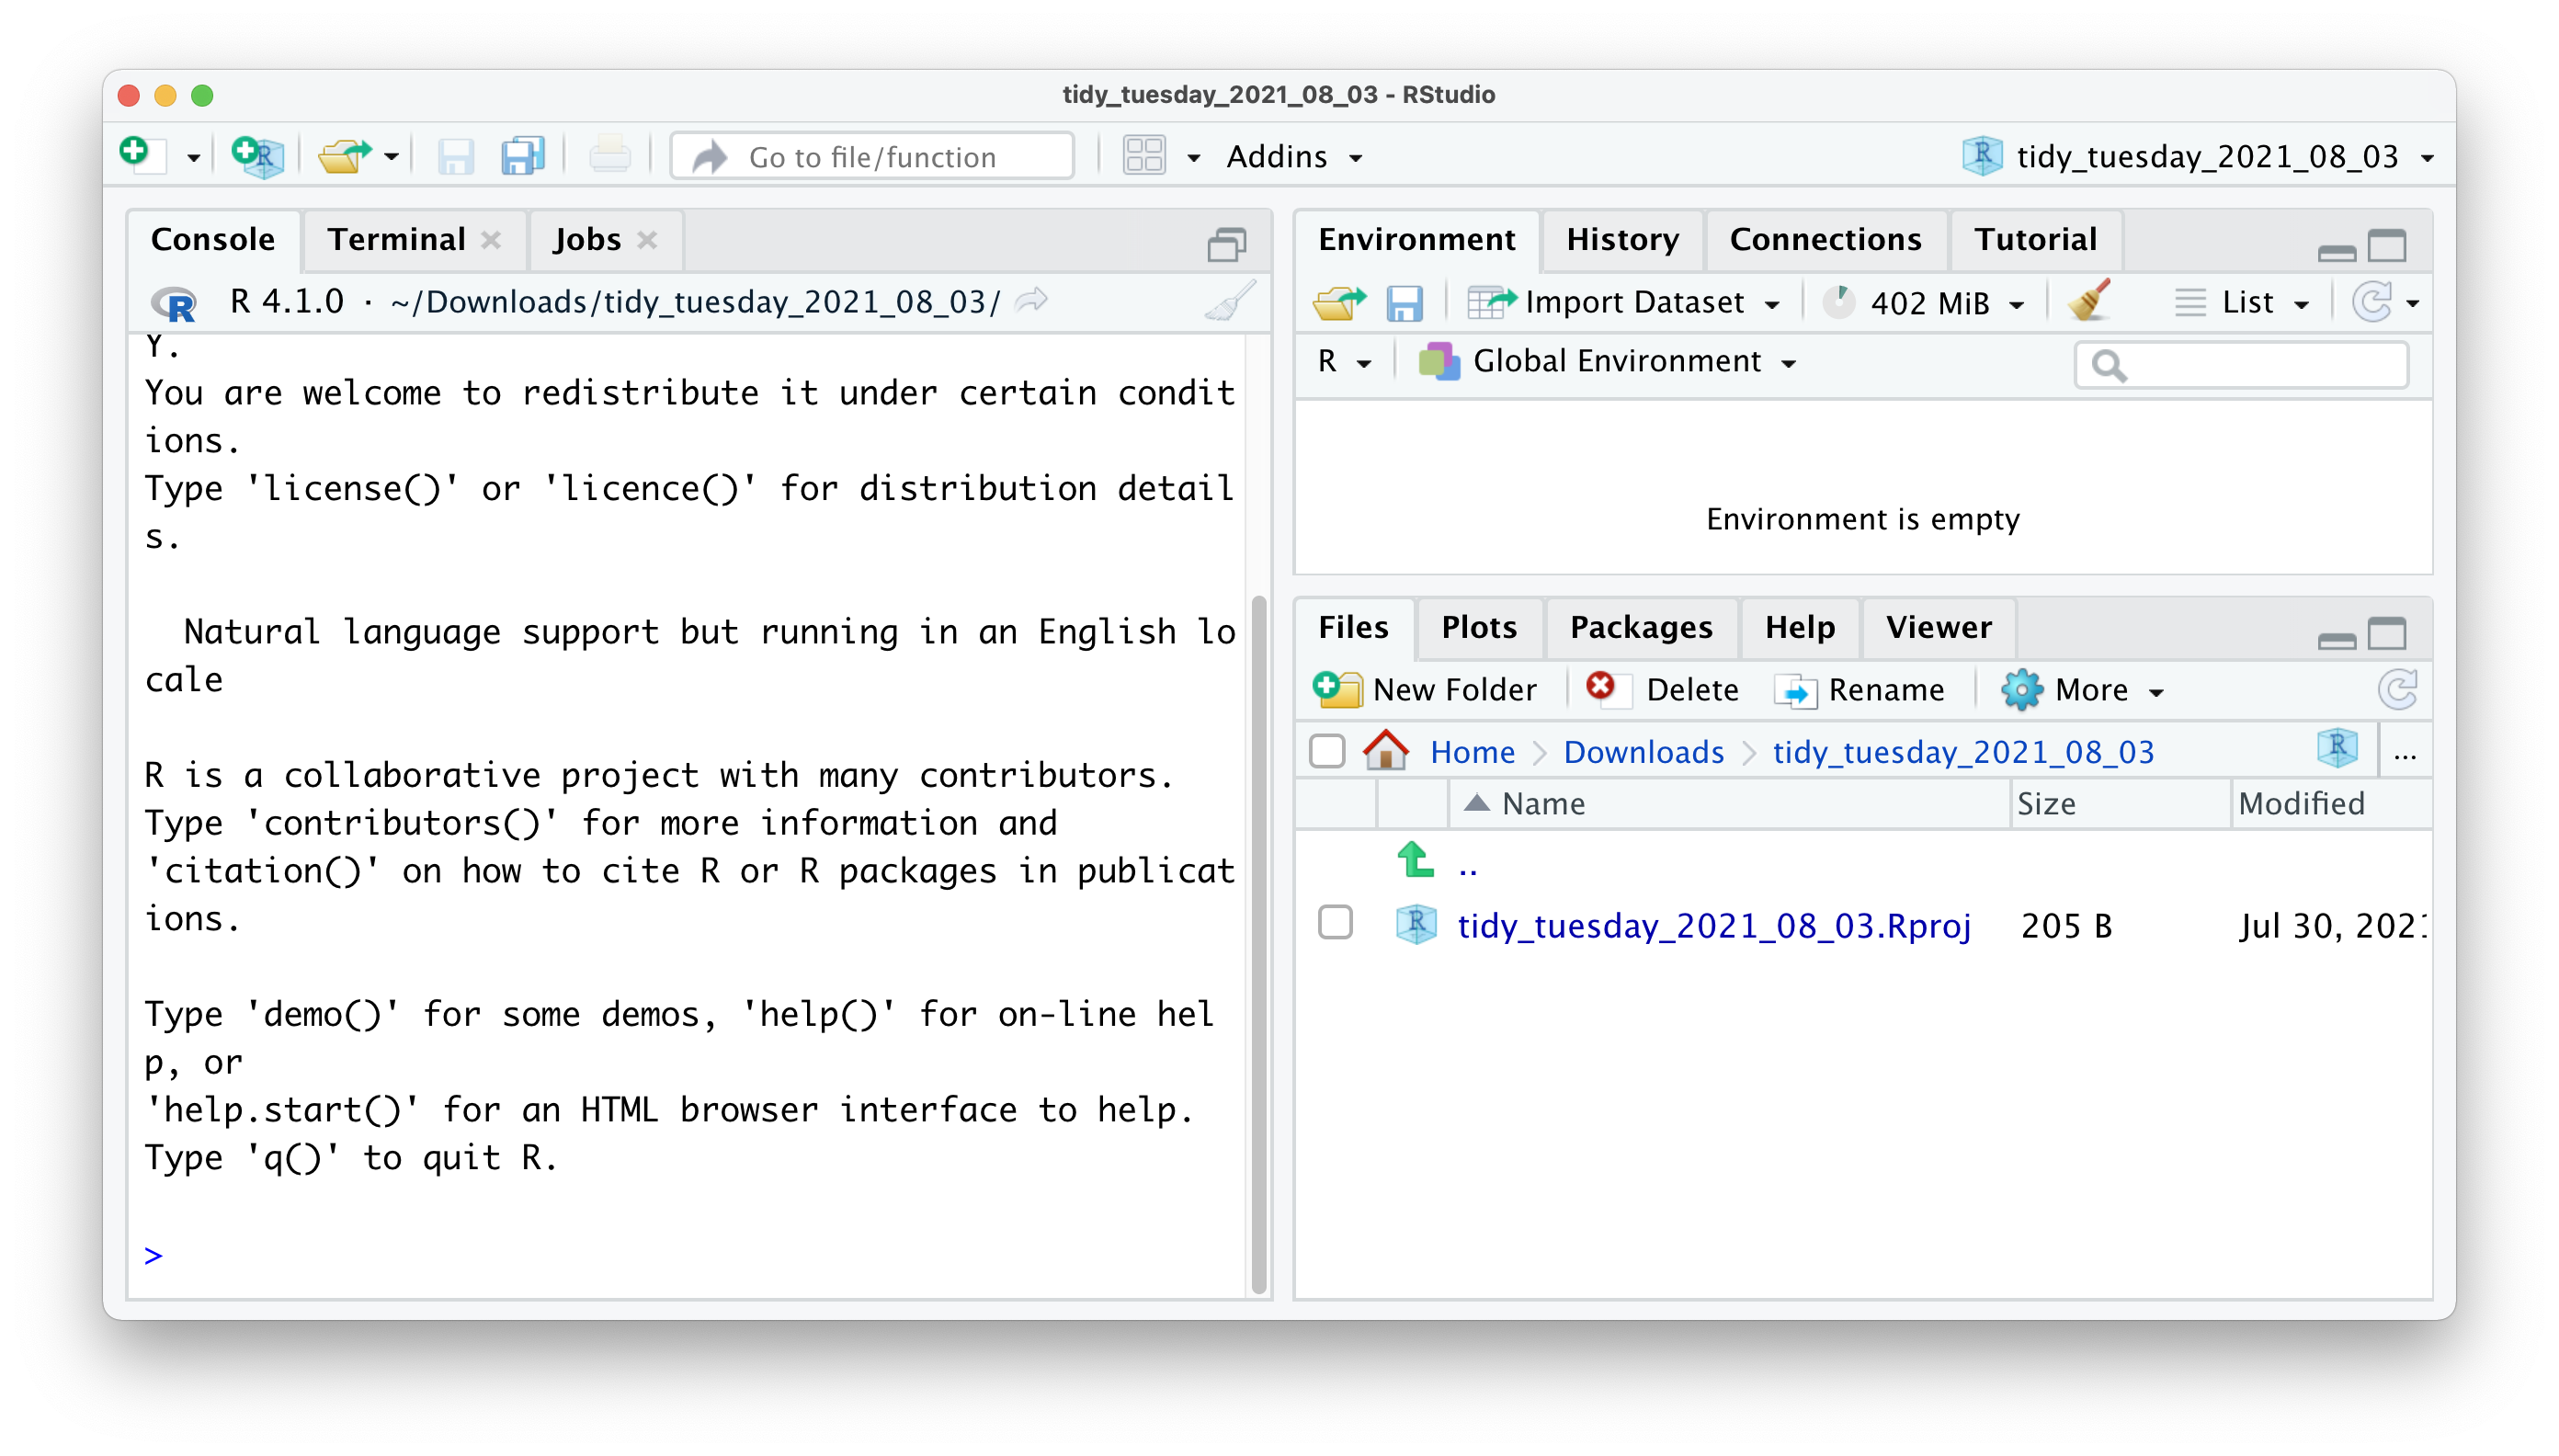
\includegraphics{images/chapter_06_img/00_r_project/05_r_project_new_session.png}
\end{enumerate}

If you look carefully, you can see that your RStudio is now `branded'
with your project name. At the top of the window, you see the project
name, the files pane shows the root directory where all your files will
be, and even the console shows on top the file path of your project. You
could set all this up manually, but I would not recommend it, not the
least because it is easy and swift to work with \emph{R} Projects.

\section{Organising your projects}\label{organising-your-projects}

This section is not directly related to RStudio, \emph{R} or data
analysis in general. Instead, I want to convey to you that a good folder
structure can go a long way. It is an excellent habit to start thinking
about folder structures before you start working on your project.
Placing your files into dedicated folders, rather than keeping them
loosely in one container, will speed up your work and save you from the
frustration of not finding the files you need. I have a template that I
use regularly. You can either create it from scratch in RStudio or open
your file browser and create the folders there. RStudio does not mind
which way you do it. If you want to spend less time setting this up, you
might want to use the function \texttt{create\_project\_folder()} from
the \texttt{r4np} package. It creates all the folders as shown in Figure
@ref(fig:folder-structure).

\begin{Shaded}
\begin{Highlighting}[]
\CommentTok{\# Install \textquotesingle{}r4np\textquotesingle{} from GitHub}
\NormalTok{devtools}\SpecialCharTok{::}\FunctionTok{install\_github}\NormalTok{(}\StringTok{"ddauber/r4np"}\NormalTok{)}

\CommentTok{\# Create the template structure}
\NormalTok{r4np}\SpecialCharTok{::}\FunctionTok{create\_project\_folder}\NormalTok{()}
\end{Highlighting}
\end{Shaded}

To create a folder, click on \texttt{New\ Folder} in the \emph{Files}
pane. I usually have at least the following folders for every project I
am involved in:

\begin{itemize}
\item
  A folder for my raw data. I store `untouched' datasets in it. With
  `untouched', I mean they have not been processed in any way and are
  usually files I downloaded from my data collection tool, e.g.~an
  online questionnaire platform.
\item
  A folder with `tidy' data. This is usually data I exported from
  \emph{R} after cleaning it, i.e.~after some basic data wrangling and
  cleaning (see Chapter @ref(data-wrangling)).
\item
  A folder for my \emph{R} scripts
\item
  A folder for my plots
\item
  A folder for reports.
\end{itemize}

Thus, in RStudio, it would look something like this:

\begin{figure}

\centering{

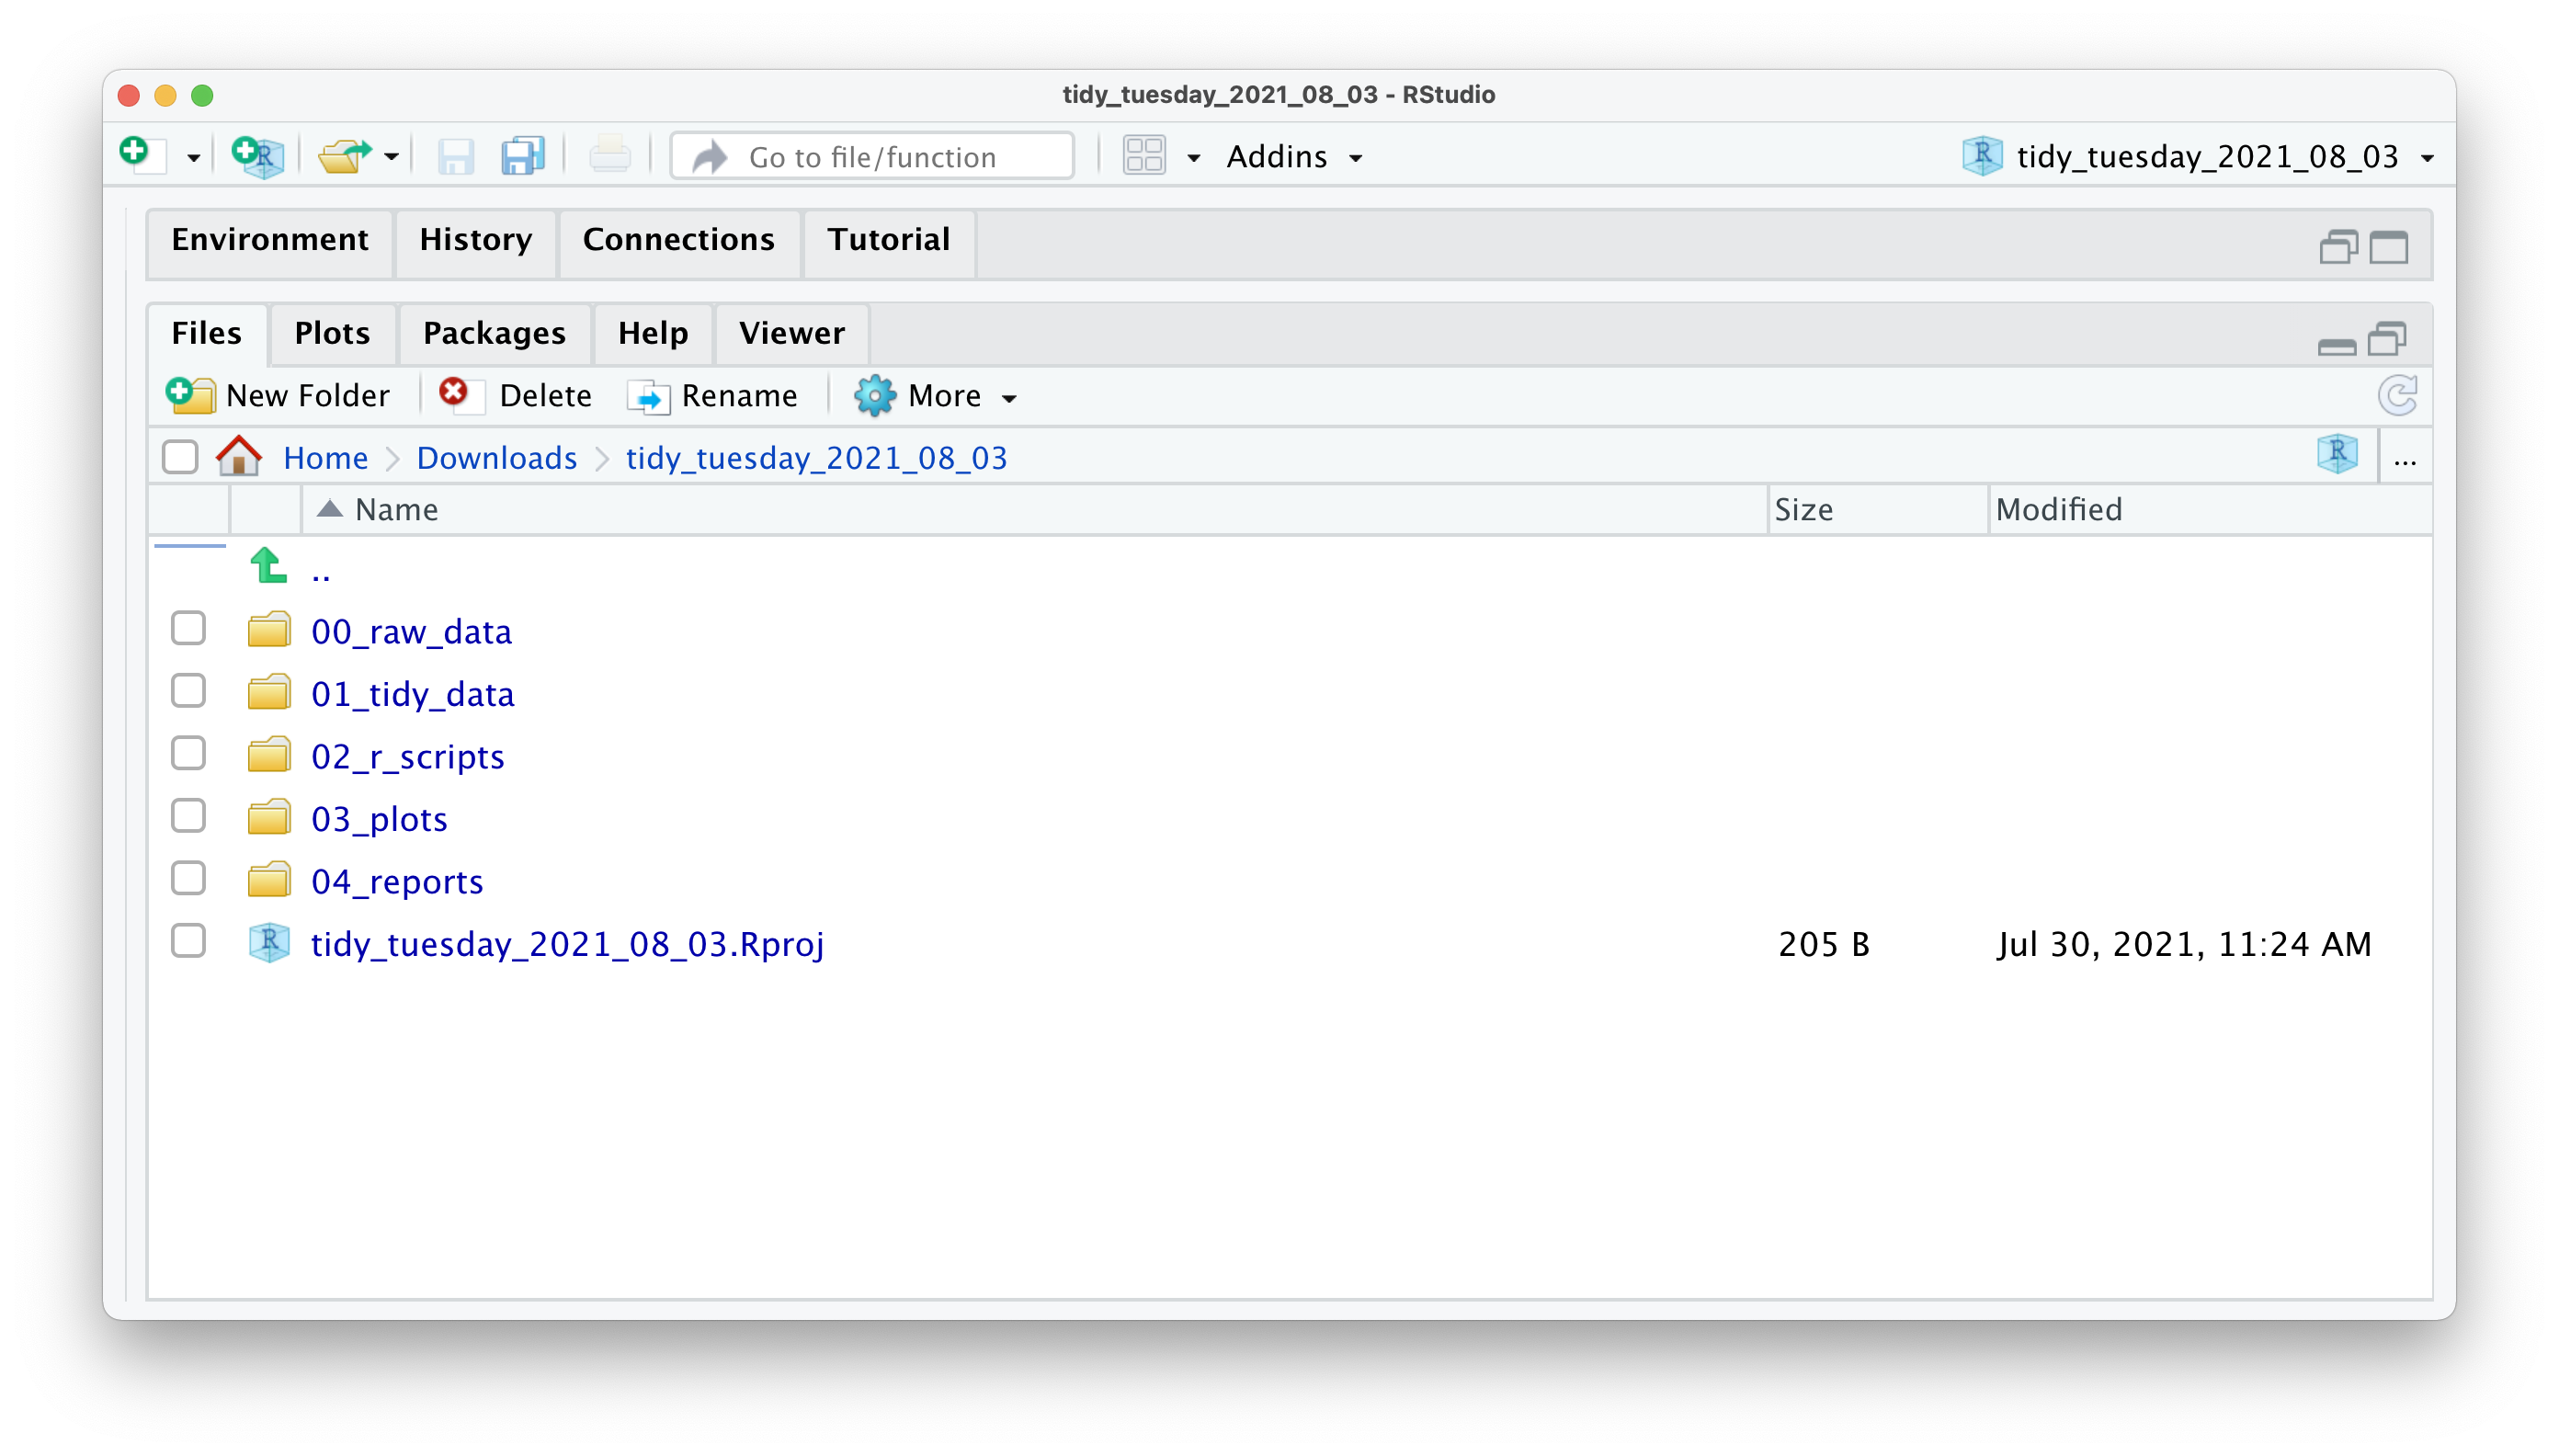
\includegraphics{images/chapter_06_img/01_organising_work/00_organising_work.png}

}

\caption{\label{fig-folder-structure}An example of a scalable folder
structure for your project}

\end{figure}%

You probably noticed that my folders have numbers in front of them. I do
this to ensure that all folders are in the order I want them to be,
which is usually not the alphabetical order my computer suggests. I use
two digits because I may have more than nine folders for a project, and
folder ten would otherwise be listed as the third folder in this list.
With this filing strategy in place, it will be easy to find whatever I
need. Even others can easily understand what I stored where. It is
simply `tidy', similar to how we want our data to be.

\section{\texorpdfstring{Creating an \emph{R}
Script}{Creating an R Script}}\label{creating-an-r-script}

Code quickly becomes long and complex. Thus, it is not very convenient
to write it in the console. So, instead, we can write code into an
\emph{R} Script. An \emph{R} Script is a document that RStudio
recognises as \emph{R} programming code. Files that are not \emph{R}
Scripts, like \texttt{.txt}, \texttt{.rtf} or \texttt{.md}, can also be
opened in RStudio, but any code written in it will not be automatically
recognised.

When opening an \emph{R} script or creating a new one, it will display
in the \emph{Source} window (see Chapter @ref(the-source-window)). Some
refer to this window as the `script editor'. An \emph{R} script starts
as an empty file. Good coding etiquette (see Chapter
@ref(coding-etiquette)) demands that we use the first line to indicate
what this file does by using a comment \texttt{\#}. Here is an example
for a \href{https://www.tidytuesday.com}{`TidyTuesday'} \emph{R}
Project.

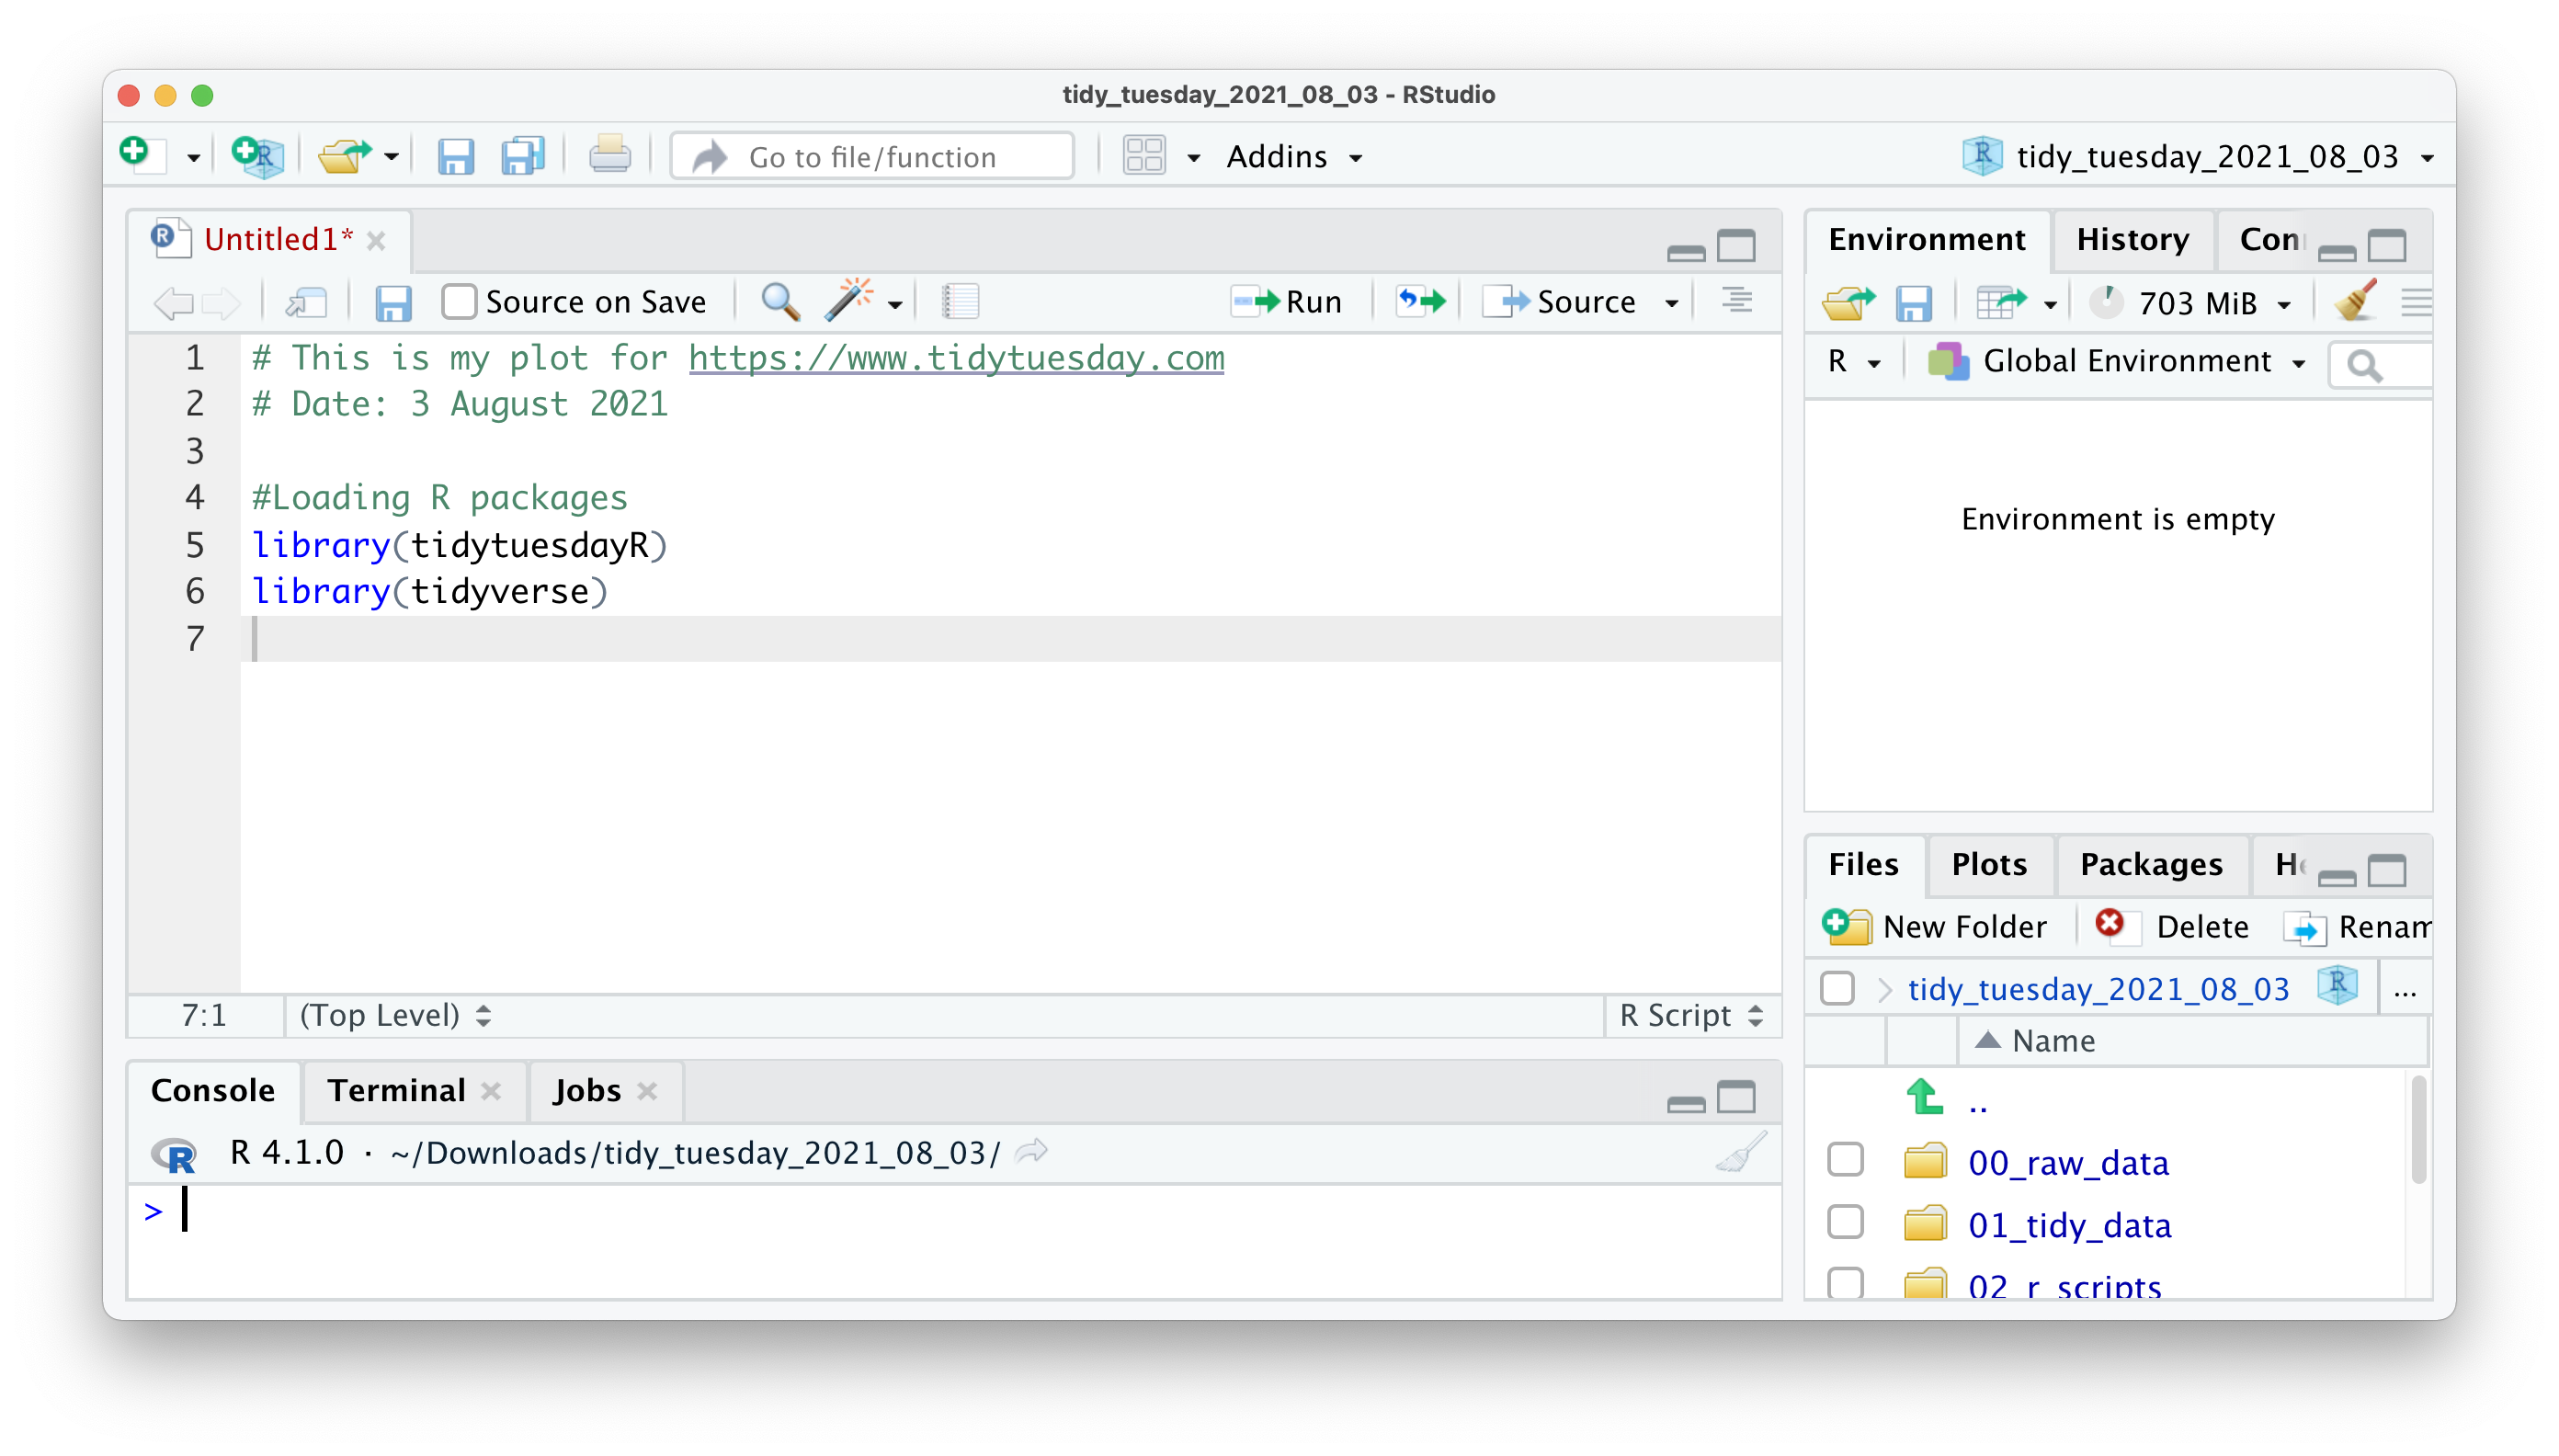
\includegraphics{images/chapter_06_img/02_r_script/00_r_script.png}

All examples in this book can easily be copied and pasted into your own
\emph{R} script. However, for some code you will have to install the
\emph{R} package \texttt{r4np} (see \hyperref[install_r4np]{above}).
Let's try it with the following code. The plot this code creates reveals
which car manufacturer produces the most efficient cars. Copy and paste
this code into your \emph{R} script.

\begin{Shaded}
\begin{Highlighting}[]
\FunctionTok{library}\NormalTok{(tidyverse)}

\NormalTok{mpg }\SpecialCharTok{\%\textgreater{}\%} \FunctionTok{ggplot}\NormalTok{(}\FunctionTok{aes}\NormalTok{(}\AttributeTok{x =} \FunctionTok{reorder}\NormalTok{(manufacturer, }\FunctionTok{desc}\NormalTok{(hwy), }\AttributeTok{FUN =}\NormalTok{ median),}
                   \AttributeTok{y =}\NormalTok{ hwy,}
                   \AttributeTok{fill =}\NormalTok{ manufacturer)) }\SpecialCharTok{+}
  \FunctionTok{geom\_boxplot}\NormalTok{() }\SpecialCharTok{+}
  \FunctionTok{coord\_flip}\NormalTok{() }\SpecialCharTok{+}
  \FunctionTok{theme\_minimal}\NormalTok{() }\SpecialCharTok{+}
  \FunctionTok{xlab}\NormalTok{(}\StringTok{"Manufacturer"}\NormalTok{) }\SpecialCharTok{+}
  \FunctionTok{ylab}\NormalTok{(}\StringTok{"Highway miles per gallon"}\NormalTok{)}
\end{Highlighting}
\end{Shaded}

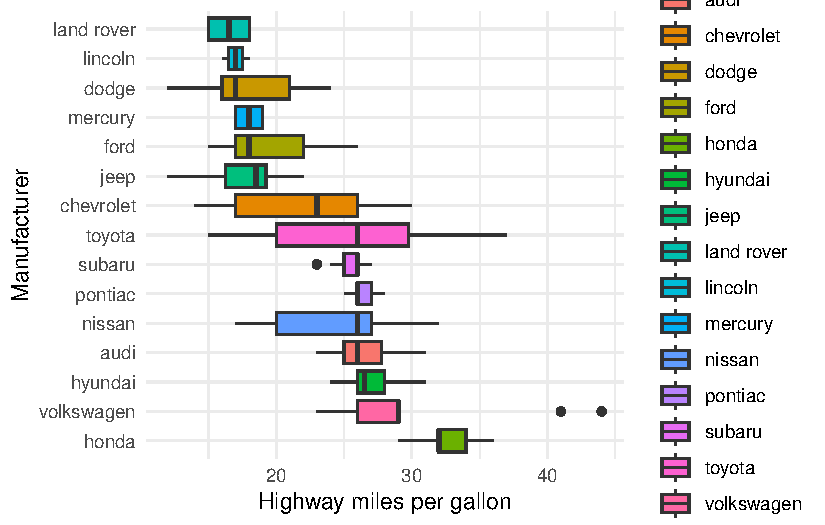
\includegraphics{06_starting_r_projects_files/figure-pdf/r-script-copy-paste-examples-1.pdf}

You are probably wondering where your plot has gone. Copying the code
will not automatically run it in your \emph{R} script. However, this is
necessary to create the plot. If you tried pressing \texttt{Return\ ↵},
you would only add a new line. Instead, you need to select the code you
want to run and press \texttt{Ctrl+Return\ ↵} (PC) or
\texttt{Cmd+Return\ ↵} (Mac). You can also use the \texttt{Run} command
at the top of your source window, but it is much more efficient to press
the keyboard shortcut. Besides, you will remember this shortcut quickly,
because we need to use it very frequently. If all worked out, you should
see the following:

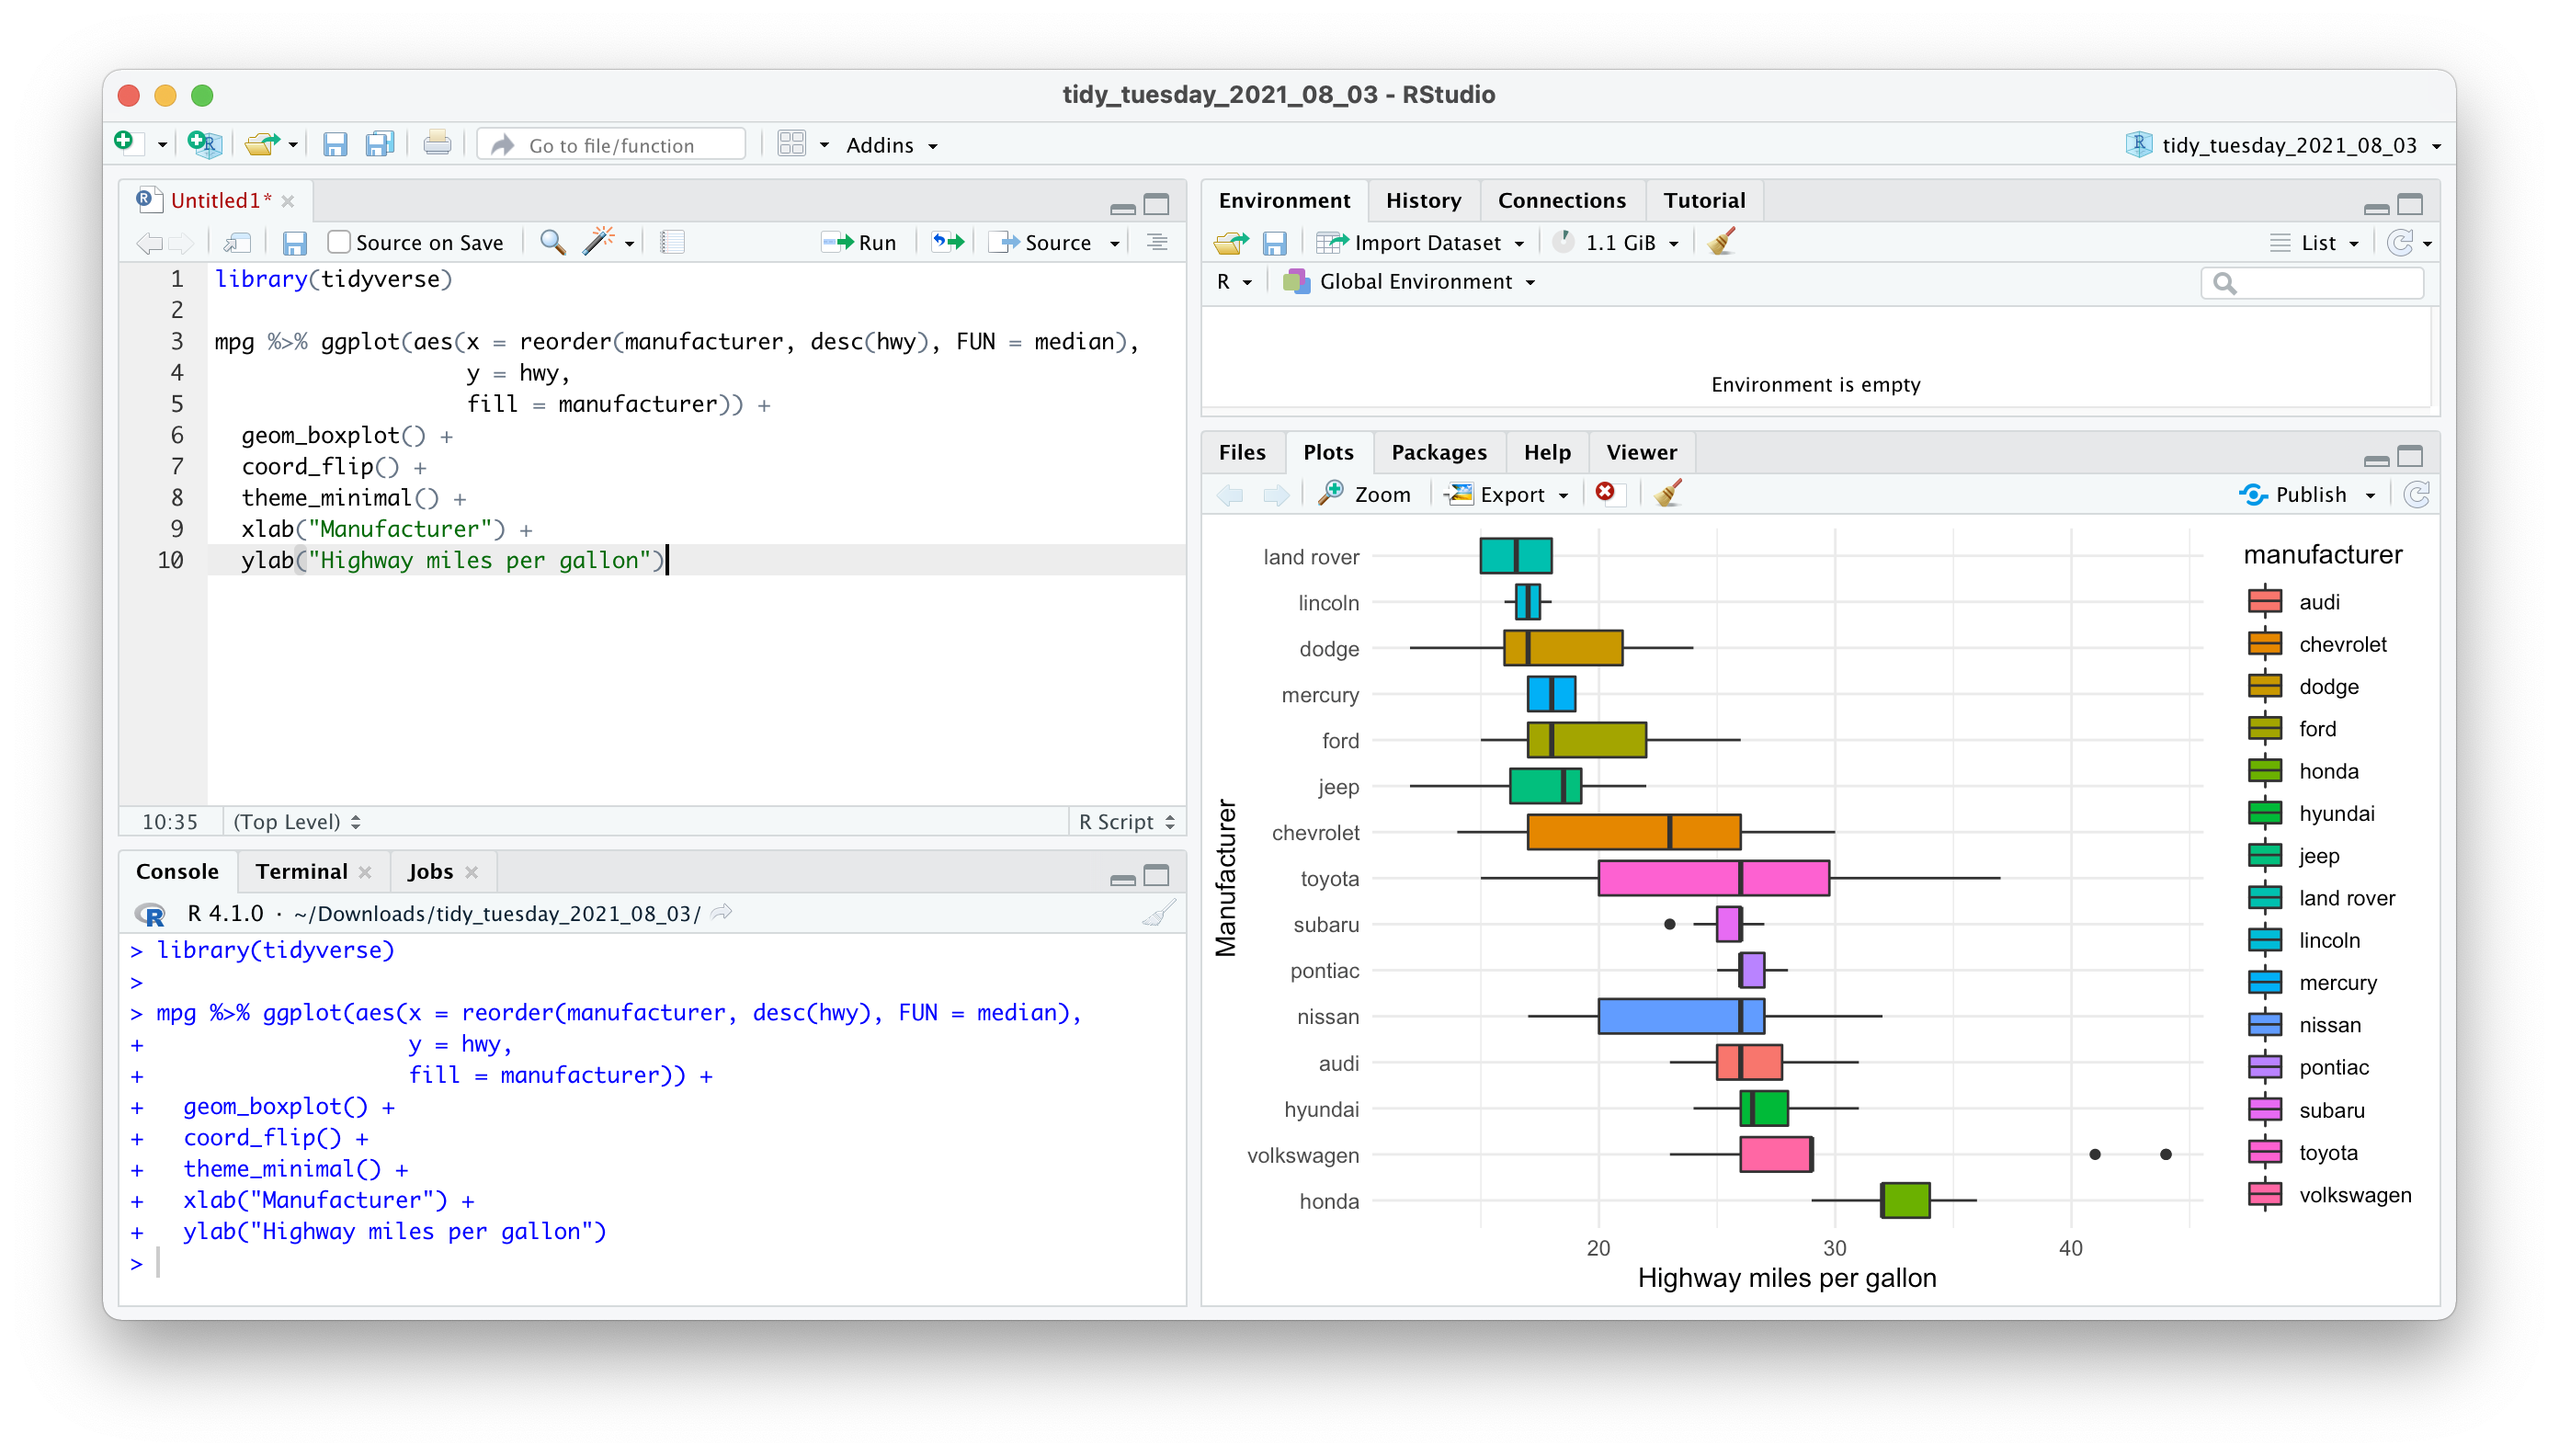
\includegraphics{images/chapter_06_img/02_r_script/01_r_script_example_plot.png}

As you can see, cars from \texttt{Honda} appear to drive furthest with
the same amount of fuel (a gallon) compared to other vehicles. Thus, if
you are looking for very economical cars, you now know where to find
them.

The \emph{R} script editor has some conveniences for writing your code
that are worth pointing out. You probably noticed that some of the code
we have pasted is blue, and some other code is in green. These colours
help to make your code more readable because they carry a specific
meaning. In the default settings, green stands for any values in
\texttt{""}, which usually stands for \texttt{character}s. Automatic
colouring of our progamming code is also called \emph{`syntax
highlighting'}.

Moreover, code in \emph{R} scripts will be automatically indented to
facilitate reading. If, for whatever reason, the indentation does not
happen, or you accidentally undo it, you can reindent a line with
\texttt{Ctrl+I} (PC) or \texttt{Cmd+I} (Mac).

Lastly, the console and the \emph{R} script editor both feature code
completion. This means that when you start typing the name of a
function, \emph{R} will provide suggestions. These are extremely helpful
and make programming a lot faster. Once you found the function you were
looking for, you press \texttt{Return\ ↵} to insert it. Here is an
example of what happens when you have the package \texttt{tidyverse}
loaded and type \texttt{ggpl}. Only functions that are loaded via
packages or any object in your environment pane benefit from code
completion.

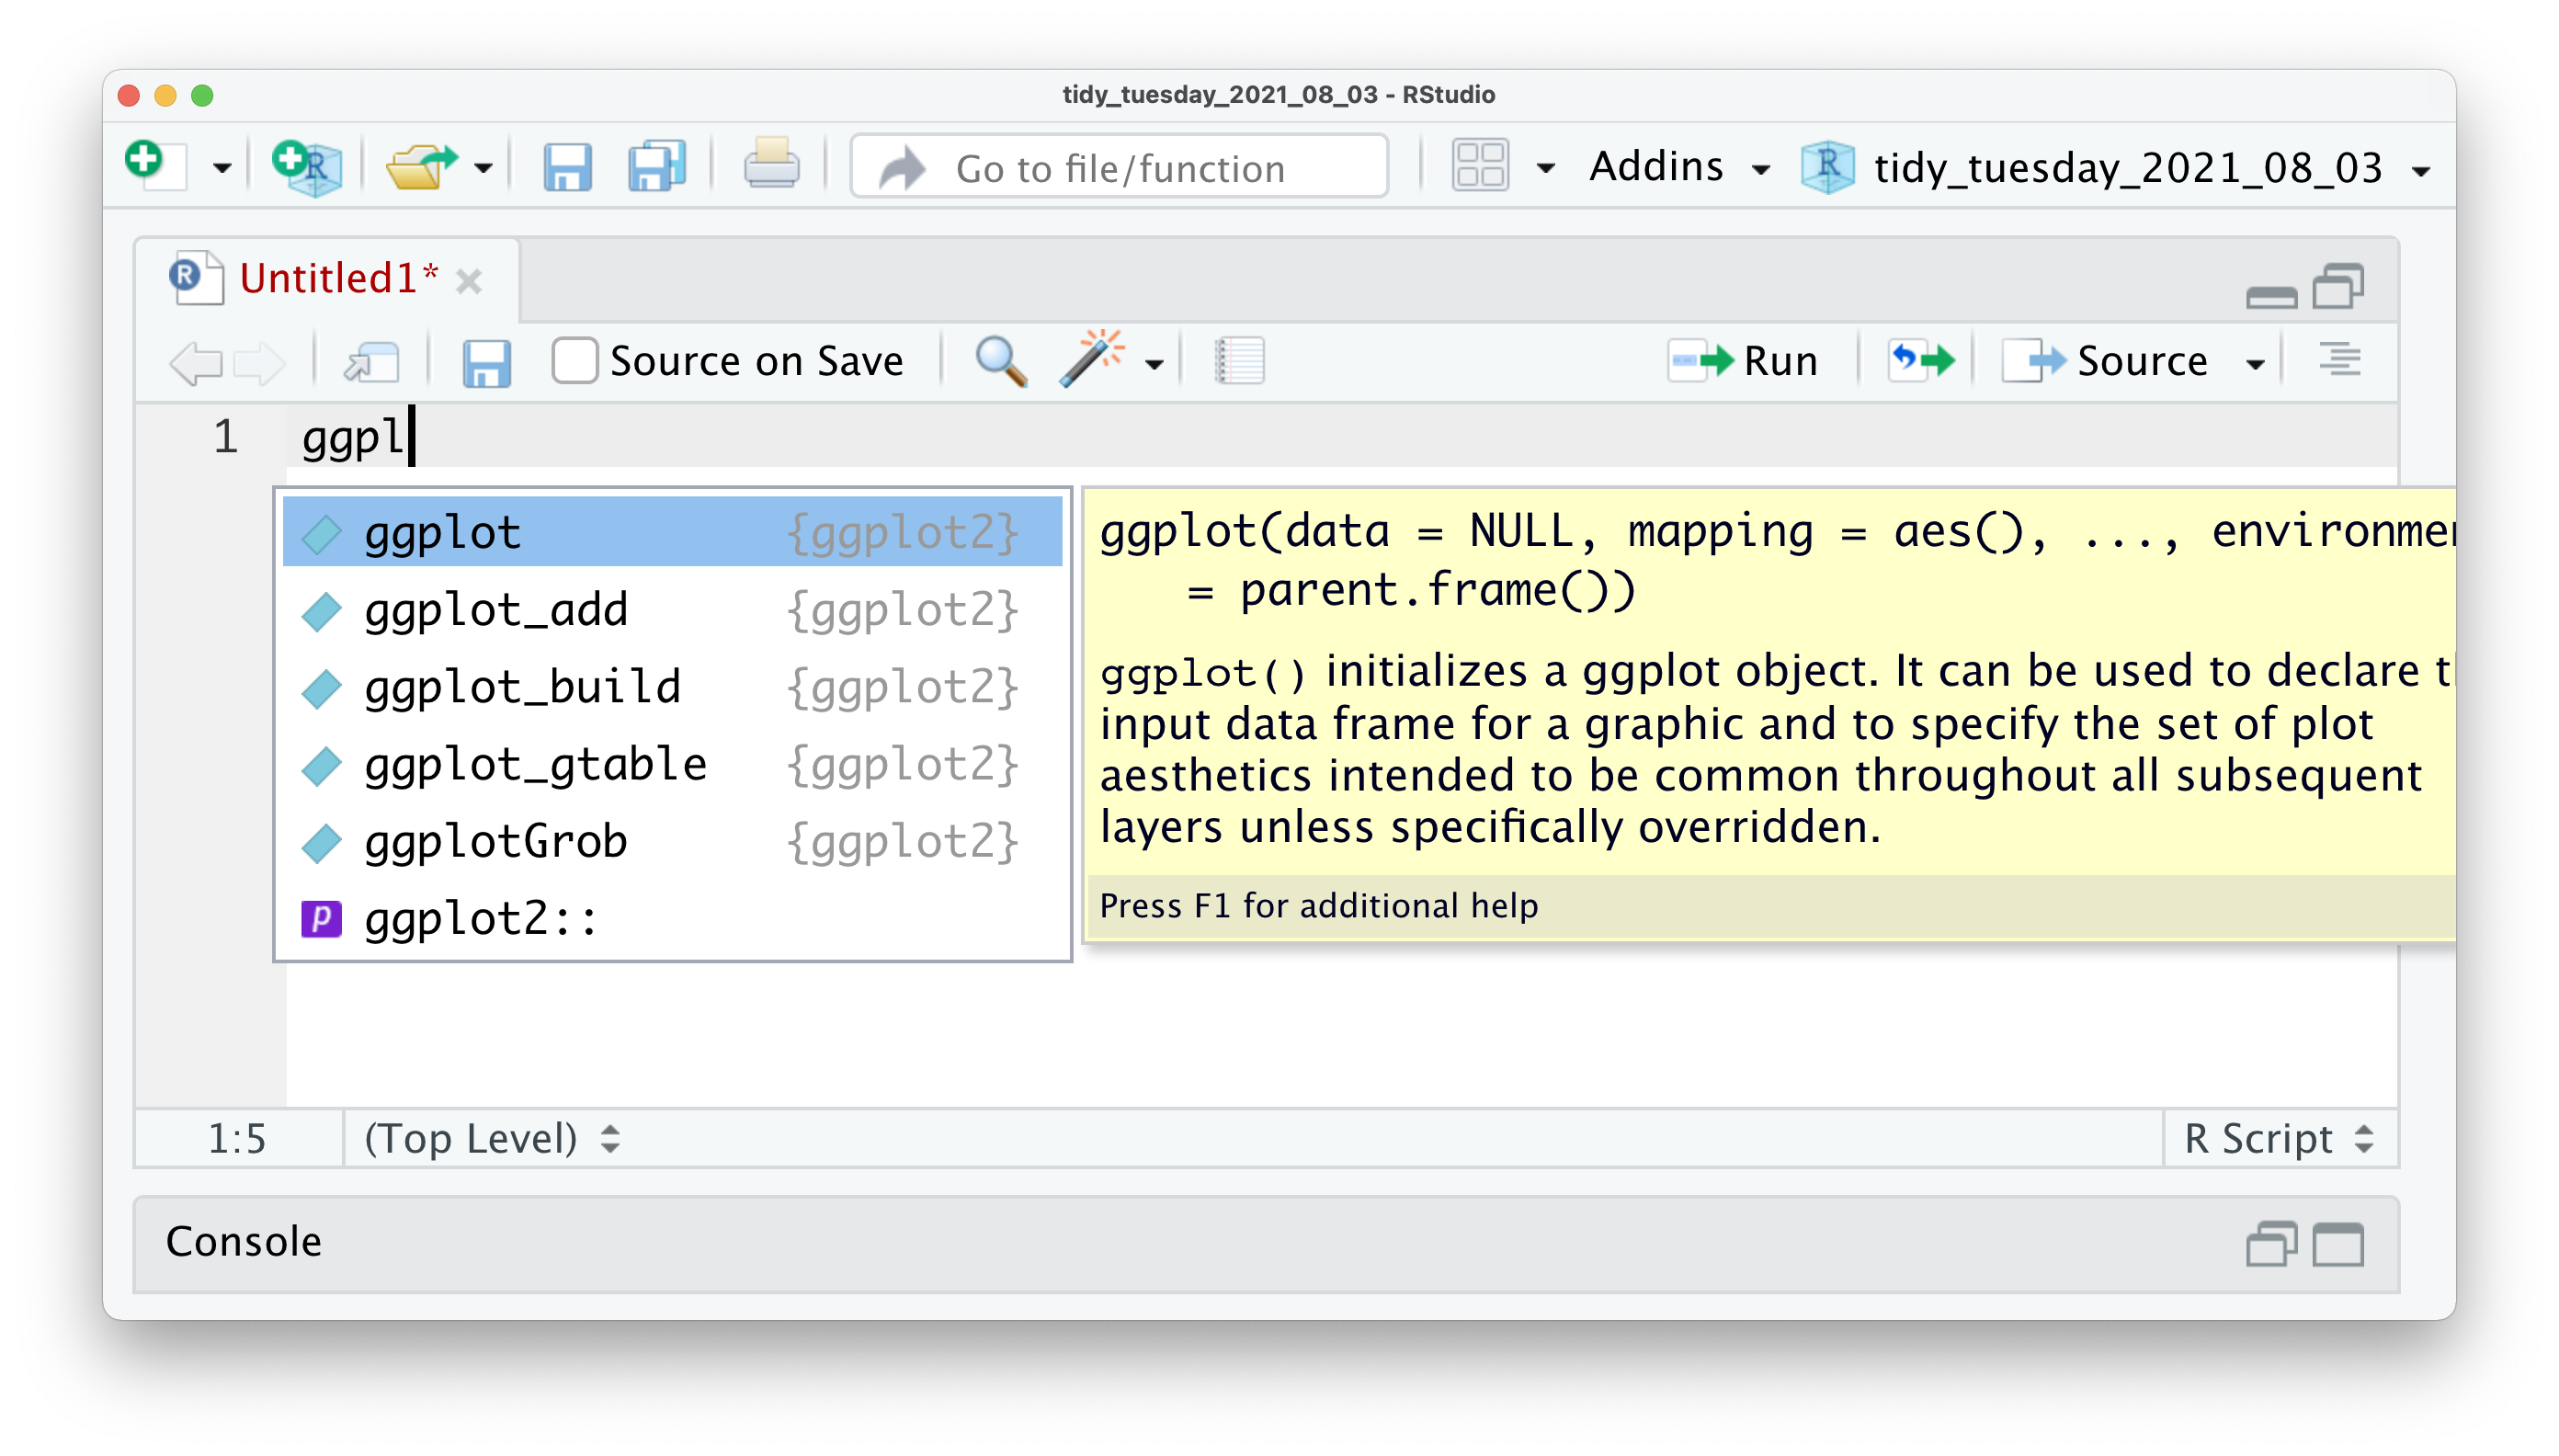
\includegraphics{images/chapter_06_img/02_r_script/02_r_script_code_completion.png}

Not only does RStudio show you all the available options, but it also
tells you which package this function is from. In this case, all listed
functions are from the \texttt{ggplot2} package. Furthermore, when you
select one of the options but have not pressed \texttt{Return\ ↵} yet,
you also get to see a yellow box, which provides you with a quick
reference of all the arguments that this function accepts. So you do not
have to memorise all the functions and their arguments.

\section{\texorpdfstring{Using \emph{R}
Markdown}{Using R Markdown}}\label{r-markdown-and-r-notebooks}

There is too much to say about \emph{R} Markdown, which is why I only
will highlight that it exists and point out the one feature that might
convince you to choose this format over plain \emph{R} scripts: They
look like a Word document (almost).

As the name indicates, \emph{R} Markdown files are a combination of
\emph{R} scripts and '\emph{Markdown'}. \emph{`Markdown'} is a way of
writing and formatting text documents without needing software like MS
Word. Instead, you write everything in plain text. Such plain text can
be converted into many different document types such as HTML websites,
PDF or Word documents. If you would like to see how it works, I
recommend looking at
the~\href{https://www.rstudio.com/resources/cheatsheets/}{R Markdown
Cheatsheet}. To create an \emph{R} Markdown file click on
\texttt{File\ \textgreater{}\ New\ File\ \textgreater{}\ R\ Markdown...}.

An \emph{R} Markdown file works oppositely to an \emph{R} script. By
default, an \emph{R} script considers everything as code and only
through commenting \texttt{\#} we can include text to describe what the
code does. This is what you have seen in all the coding examples so far.
On the other hand, an \emph{R} Markdown file considers everything as
text, and we have to specify what is code. We can do so by inserting
\emph{`code chunks'}. Therefore, there is less of a need to use comments
\texttt{\#} in \emph{R} Markdown files because you can write about it.
Another convenience of \emph{R} Markdown files is that results from your
analysis are immediately shown underneath the code chunk and not in the
console.

\includegraphics{images/chapter_06_img/03_r_markdown/01_r_markdown_plain.png}

If you switch your view to the \texttt{Visual\ Editor}, it almost looks
like you are writing a report in MS Word.

\includegraphics{images/chapter_06_img/03_r_markdown/02_r_markdown_visual_editor_menu.png}

\includegraphics{images/chapter_06_img/03_r_markdown/03_r_markdown_visual_editor.png}

So, when should you use an \emph{R} script, and when should you use
\emph{R} Markdown. The rule-of-thumb is that if you intend to write a
report, thesis or another form of publication, it might be better to
work in an \emph{R} Markdown file. If this does not apply, you might
want to use an \emph{R} Script. As mentioned above, \emph{R} Markdown
files emphasise text, while \emph{R} scripts primarily focus on code. In
my projects, I often have a mixture of both. I use \emph{R} Scripts to
carry out data wrangling and my primary analysis and then use \emph{R}
Markdown files to present the findings, e.g.~creating plots, tables, and
other components of a report. By the way, this book is written in
\emph{R} Markdown using the \texttt{bookdown} package.

No matter your choice, it will neither benefit nor disadvantage you in
your \emph{R} journey or when working through this book. The choice is
all yours. You likely will come to appreciate both formats for what they
offer. If you want to find out more about \emph{R} Markdown and how to
use it, I highly recommend taking a look at
\href{https://bookdown.org/yihui/rmarkdown/}{`R Markdown: The Definitive
Guide'} (Xie, Allaire, and Grolemund 2018).

\bookmarksetup{startatroot}

\chapter{Data Wrangling}\label{data-wrangling}

\begin{quote}
\textbf{Data wrangling} --- also called~\textbf{data
cleaning},~\textbf{data remediation}, or~\textbf{data munging}---refers
to a variety of processes designed to transform raw data into more
readily used formats. The exact methods differ from project to project
depending on the data you're leveraging and the goal you're trying to
achieve. (Stobierski 2021)
\end{quote}

You collected your data over months (and sometimes years), and all you
want to know is whether your data makes sense and reveals something
nobody would have ever expected. However, before we can truly go ahead
with our analysis, it is essential to understand whether our data is
`tidy'. What I mean is that our data is at the quality we would expect
it to be and can be reliably used for data analysis. After all, the
results of our research are only as good as our data and the methods we
deploy to achieve the desired insights.

Very often, the data we receive is everything else but clean, and we
need to check whether our data is fit for analysis and ensure it is in a
format that is easy to handle. For small datasets, this is usually a
brief exercise. However, I found myself cleaning data for a month
because the dataset was spread out into multiple spreadsheets with
different numbers of columns and odd column names that were not
consistent. Thus, data wrangling is an essential first step in any data
analysis. It is a step that cannot be skipped and has to be performed on
every new dataset. If your background is in qualitative research, you
likely conducted interviews which you had to transcribe. The process of
creating transcriptions is comparable to data wrangling in quantitative
datasets - and equally tedious.

Luckily, \emph{R} provides many useful functions to make our lives
easier. You will be in for a treat if you are like me and used to do
this in Excel. It is a lot simpler using \emph{R} to achieve a clean
dataset.

Here is an overview of the different steps we usually work through
before starting with our primary analysis. This list is certainly not
exhaustive:

\begin{itemize}
\item
  Import data,
\item
  Check data types,
\item
  Recode and arrange factors, i.e.~categorical data, and
\item
  Run missing data diagnostics.
\end{itemize}

\section{Import your data}\label{import-your-data}

The \texttt{r4np} package hosts several different datasets to work with,
but at some point, you might want to apply your \emph{R} knowledge to
your own data. Therefore, an essential first step is to import your data
into RStudio. There are three different methods, all of which are very
handy:

\begin{enumerate}
\def\labelenumi{\arabic{enumi}.}
\item
  Click on your data file in the \emph{Files} pane and choose
  \texttt{Import\ Dataset}.
\item
  Use the \texttt{Import\ Dataset} button in the \emph{Environment}
  pane.
\item
  Import your data calling one of the \texttt{readr} functions in the
  \emph{Console} or \emph{R} script.
\end{enumerate}

We will use the \texttt{readr} package or all three options. Using this
package we can import a range of different file formats, including
\texttt{.csv}, \texttt{.tsv}, \texttt{.txt}. If you want to import data
from an \texttt{.xlsx} file, you need to use another package called
\texttt{readxl}. Similarly, if you used SPSS, Stata or SAS files before
and want to use them in \emph{R} you can use the \texttt{haven} package.
The following sections will primarily focus on using \texttt{readr} via
RStudio or directly in your \emph{Console} or \emph{R} script.

\subsection{\texorpdfstring{Import data from the \emph{Files}
pane}{Import data from the Files pane}}\label{import-data-from-the-files-pane}

This approach is by far the easiest. Let's assume you have a dataset
called \texttt{gender\_age.csv} in your \texttt{00\_raw\_data} folder.
If you wish to import it, you can do the following:

\begin{enumerate}
\def\labelenumi{\arabic{enumi}.}
\item
  Click on the name of the file.
\item
  Select \texttt{Import\ Dataset}.

  \includegraphics{images/chapter_07_img/01_files_pane_import/01_files_pane_import.png}
\item
  A new window will open, and you can choose different options. You also
  see a little preview of how the data looks like. This is great if you
  are not sure whether you did it correctly.

  \includegraphics{images/chapter_07_img/01_files_pane_import/02_files_pane_import.png}
\item
  You can change how data should be imported, but the default should be
  fine in most cases. Here is a quick breakdown of the most important
  options:

  \begin{itemize}
  \item
    \texttt{Name} allows you to change the object name, i.e.~the name of
    the object this data will be assigned to. I often use
    \texttt{df\_raw} (\texttt{df} stand for \texttt{data\ frame}, which
    is how \emph{R} calls such rectangular datasets).
  \item
    \texttt{Skip} is helpful if your data file starts with several empty
    rows at the top. You can remove them here.
  \item
    \texttt{First\ Row\ as\ Names} is ticked by default. In most Social
    Science projects, we tend to have the name of the variables as the
    first row in our dataset.
  \item
    \texttt{Trim\ Spaces} removes any unnecessary whitespace in your
    dataset. Leave it ticked.
  \item
    \texttt{Open\ Data\ Viewer} allows you to look at your imported
    dataset. I use it rarely, but it can be helpful at times.
  \item
    \texttt{Delimiter} defines how your columns are separated from each
    other in your file. If it is a \texttt{.csv} file, it would imply it
    is a `comma-separated value', i.e.~\texttt{,}. This setting can be
    changed for different files, depending on how your data is
    delimited. You can even use the option \texttt{Other…} to specify a
    custom separation option.
  \item
    \texttt{NA} specifies how missing values in your data are
    acknowledged. By default, empty cells in your data will be
    recognised as missing data.
  \end{itemize}

  \includegraphics{images/chapter_07_img/01_files_pane_import/03_files_pane_import.png}
\item
  Once you are happy with your choices, you can click on
  \texttt{Import}.
\item
  You will find your dataset in the \emph{Environment} pane.

  \includegraphics{images/chapter_07_img/01_files_pane_import/04_files_pane_import.png}
\end{enumerate}

In the \emph{Console}, you can see that \emph{R} also provides the
\texttt{Column\ specification}, which we need later when inspecting
`data types'. \texttt{readr} automatically imports all text-based
columns as \texttt{chr}, i.e.~\texttt{character} values. However, this
might not always be the correct data type. We will cover more of this
aspect of data wrangling in Chapter @ref(change-data-types).

\subsection{\texorpdfstring{Importing data from the \emph{Environment}
pane}{Importing data from the Environment pane}}\label{importing-data-from-the-environment-pane}

The process of importing datasets from the \emph{Environment} pane
follows largely the one from the \emph{Files} pane. Click on
\texttt{Import\ Dataset\ \textgreater{}\ From\ Text\ (readr)…}. The only
main difference lies in having to find the file using the
\texttt{Browse…} button. The rest of the steps are the same as above.

Be aware that you will have to use the \emph{Environment} pane for
importing data from specific file types, e.g.~\texttt{.txt}. The
\emph{File} pane would only open the file but not import the data for
further processing.

\subsection{Importing data using functions
directly}\label{importing-data-using-functions}

If you organised your files well, it could be effortless and quick to
use all the functions from \texttt{readr} directly. Here are two
examples of how you can use \texttt{readr} to import your data. Make
sure you have the package loaded.

\begin{Shaded}
\begin{Highlighting}[]
\CommentTok{\# Import data from \textquotesingle{}.csv\textquotesingle{}}
\FunctionTok{read\_csv}\NormalTok{(}\StringTok{"00\_raw\_data/gender\_age.csv"}\NormalTok{)}

\CommentTok{\# Import data from any text file by defining the separator}
\FunctionTok{read\_delim}\NormalTok{(}\StringTok{"00\_raw\_data/gender\_age.txt"}\NormalTok{, }\AttributeTok{delim =} \StringTok{"|"}\NormalTok{)}
\end{Highlighting}
\end{Shaded}

You might be wondering whether you can use \texttt{read\_delim()} to
import \texttt{.csv} files too. The answer is `Yes, you can!'. In
contrast to \texttt{read\_delim()}, \texttt{read\_csv()} sets the
delimiter to \texttt{,} by default. This is mainly for convenience
because \texttt{.csv} files are one of the most popular file formats
used to store data.

You might also be wondering what a \emph{`delimiter'} is. When you
record data in a plain-text file, it is easy to see where a new
observation starts and ends because it is defined by a row in your file.
However, we also need to tell our software where a new column starts,
i.e.~where a cell begins and ends. Consider the following example. We
have a file that holds our data which looks like this:

\begin{verbatim}
idagegender
124male
256female
333male
\end{verbatim}

The first row we probably can still decipher as \texttt{id},
\texttt{age}, \texttt{gender}. However, the next row makes it difficult
to understand which value represents the \texttt{id} of a participant
and which value reflects the \texttt{age} of that participant. Like us,
computer software would find it hard too to decide on this ambiguous
content. Thus, we need to use delimiters to make it very clear which
value belongs to which column. For example, in a \texttt{.csv} file, the
data would be separated by a \texttt{,}.

\begin{verbatim}
id,age,gender
1,24,male
2,56,female
3,33,male
\end{verbatim}

Considering our example from above, we could also use
\texttt{\textbar{}} as a delimiter, but this is very unusual.

\begin{verbatim}
id|age|gender
1|24|male
2|56|female
3|33|male
\end{verbatim}

There is a lot more to \texttt{readr} than could be covered in this
book. If you want to know more about this \emph{R} package, I highly
recommend looking at the \href{https://readr.tidyverse.org}{readr
webpage}.

\section{Inspecting your data}\label{inspecting-raw-data}

For the rest of this chapter, we will use the \texttt{wvs} dataset from
the \texttt{r4np} package. However, we do not know much about this
dataset, and therefore we cannot ask any research questions worth
investigating. Therefore, we need to look at what it contains. The first
method of inspecting a dataset is to type the name of the object,
i.e.~\texttt{wvs}.

\begin{Shaded}
\begin{Highlighting}[]
\CommentTok{\# Ensure you loaded the \textquotesingle{}r4np\textquotesingle{} package first}
\FunctionTok{library}\NormalTok{(r4np)}

\CommentTok{\# Show the data in the console}
\NormalTok{wvs}
\end{Highlighting}
\end{Shaded}

\begin{verbatim}
# A tibble: 69,578 x 7
   `Participant ID` `Country name` Gender   Age relationship_status       
              <dbl> <chr>           <dbl> <dbl> <chr>                     
 1         20070001 Andorra             1    60 married                   
 2         20070002 Andorra             0    47 living together as married
 3         20070003 Andorra             0    48 separated                 
 4         20070004 Andorra             1    62 living together as married
 5         20070005 Andorra             0    49 living together as married
 6         20070006 Andorra             1    51 married                   
 7         20070007 Andorra             1    33 married                   
 8         20070008 Andorra             0    55 widowed                   
 9         20070009 Andorra             1    40 single                    
10         20070010 Andorra             1    38 living together as married
# i 69,568 more rows
# i 2 more variables: Freedom.of.Choice <dbl>, `Satisfaction-with-life` <dbl>
\end{verbatim}

The result is a series of rows and columns. The first information we
receive is: \texttt{A\ tibble:\ 69,578\ x\ 7}. This indicates that our
dataset has 69,578 observations (i.e.~rows) and 9 columns
(i.e.~variables). This rectangular format is the one we encounter most
frequently in Social Sciences (and probably beyond). If you ever worked
in Microsoft Excel, this format will look familiar. However, rectangular
data is not necessarily \texttt{tidy} data. Wickham (2014) (p.~4)
defines tidy data as follows:

\begin{quote}
\begin{enumerate}
\def\labelenumi{\arabic{enumi}.}
\tightlist
\item
  Each variable forms a column.
\item
  Each observation forms a row.
\item
  Each type of observational unit forms a table.
\end{enumerate}
\end{quote}

Even though it might be nice to look at a tibble in the console, it is
not particularly useful. Depending on your monitor size, you might only
see a small number of columns, and therefore we do not get to see a
complete list of all variables. In short, we hardly ever will find much
use in inspecting data this way. Luckily other functions can help us.

If you want to see each variable covered in the dataset and their data
types, you can use the function \texttt{glimpse()} from the
\texttt{dplyr} package which is loaded as part of the \texttt{tidyverse}
package.

\begin{Shaded}
\begin{Highlighting}[]
\FunctionTok{glimpse}\NormalTok{(wvs)}
\end{Highlighting}
\end{Shaded}

\begin{verbatim}
Rows: 69,578
Columns: 7
$ `Participant ID`         <dbl> 20070001, 20070002, 20070003, 20070004, 20070~
$ `Country name`           <chr> "Andorra", "Andorra", "Andorra", "Andorra", "~
$ Gender                   <dbl> 1, 0, 0, 1, 0, 1, 1, 0, 1, 1, 0, 0, 1, 1, 1, ~
$ Age                      <dbl> 60, 47, 48, 62, 49, 51, 33, 55, 40, 38, 54, 3~
$ relationship_status      <chr> "married", "living together as married", "sep~
$ Freedom.of.Choice        <dbl> 10, 9, 9, 9, 8, 10, 10, 8, 8, 10, 9, 8, 10, 7~
$ `Satisfaction-with-life` <dbl> 10, 9, 9, 8, 7, 10, 5, 8, 8, 10, 8, 8, 10, 7,~
\end{verbatim}

The output of glimpse shows us the name of each column/variable after
the \texttt{\$}, for example,
\texttt{\textasciigrave{}Participant\ ID\textasciigrave{}}. The
\texttt{\$} is used to lookup certain variables in our dataset. For
example, if we want to inspect the column \texttt{relationship\_status}
only, we could write the following:

\begin{Shaded}
\begin{Highlighting}[]
\NormalTok{wvs}\SpecialCharTok{$}\NormalTok{relationship\_status}
\end{Highlighting}
\end{Shaded}

\begin{verbatim}
    [1] "married"                    "living together as married"
    [3] "separated"                  "living together as married"
    [5] "living together as married" "married"                   
    [7] "married"                    "widowed"                   
....
\end{verbatim}

When using \texttt{glimpse()} we find the recognised data type for each
column, i.e.~each variable, in \texttt{\textless{}...\textgreater{}},
for example \texttt{\textless{}chr\textgreater{}}. We will return to
data types in Chapter @ref(change-data-types). Lastly, we get examples
of the values included in each variable. This output is much more
helpful.

I use \texttt{glimpse()} very frequently for different purposes, for
example:

\begin{itemize}
\item
  to understand what variables are included in a dataset,
\item
  to check the correctness of data types,
\item
  to inspect variable names for typos or unconventional names,
\item
  to look up variable names.
\end{itemize}

There is one more way to inspect your data and receive more information
about it by using a specialised \emph{R} package. The \texttt{skimr}
package is excellent in `skimming' your dataset. It provides not only
information about variable names and data types but also provides some
descriptive statistics. If you installed the \texttt{r4np} package and
called the function \texttt{install\_r4np()}, you will have
\texttt{skimr} installed already.

\begin{Shaded}
\begin{Highlighting}[]
\NormalTok{skimr}\SpecialCharTok{::}\FunctionTok{skim}\NormalTok{(wvs)}
\end{Highlighting}
\end{Shaded}

The output in the \emph{Console} should look like this:

\includegraphics{images/chapter_07_img/02_skimr_output/skimr_output.png}

As you can tell, there is a lot more information in this output. Many
descriptive statistics that could be useful are already displayed.
\texttt{skim()} provides a summary of the dataset and then automatically
sorts the variables by data type. Depending on the data type, you also
receive different descriptive statistics. As a bonus, the function also
provides a histogram for numeric variables. However, there is one main
problem: Some of the numeric variables are not numeric:
\texttt{Participant\ ID} and \texttt{Gender}. Thus, we will have to
correct the data types in a moment.

Inspecting your data in this way can be helpful to get a better
understanding of what your data includes and spot problems with it. In
addition, if you receive data from someone else, these methods are an
excellent way to familiarise yourself with the dataset relatively
quickly. Since I prepared this particular dataset for this book, I also
made sure to provide documentation for it. You can access it by using
\texttt{?wvs} in the \emph{Console}. This will open the documentation in
the \emph{Help} pane. Such documentation is available for every dataset
we use in this book.

\section{\texorpdfstring{Cleaning your column names: Call the
\texttt{janitor}}{Cleaning your column names: Call the janitor}}\label{colnames-cleaning}

If you have eagle eyes, you might have noticed that most of the variable
names in \texttt{wvs} are not consistent or easy to read/use.

\phantomsection\label{messy_column_names}%
\begin{Shaded}
\begin{Highlighting}[]
\CommentTok{\# Whitespace and inconsistent capitalisation}
\NormalTok{Participant ID        }
\NormalTok{Country name          }
\NormalTok{Gender                }
\NormalTok{Age                   }

\CommentTok{\# Difficult to read}
\NormalTok{Freedom.of.Choice     }
\NormalTok{Satisfaction}\SpecialCharTok{{-}}\NormalTok{with}\SpecialCharTok{{-}}\NormalTok{life}
\end{Highlighting}
\end{Shaded}

From Chapter @ref(coding-etiquette), you will remember that being
consistent in writing your code and naming your objects is essential.
The same applies, of course, to variable names. \emph{R} will not break
using the existing names, but it will save you a lot of frustration if
we take a minute to clean the names and make them more consistent. Since
we will use column names in almost every line of code we produce, it is
best to standardise them and make them easier to read and write.

You are probably thinking: ``This is easy. I just open the dataset in
Excel and change all the column names.'' Indeed, it would be a viable
and easy option, but it is not very efficient, especially with larger
datasets with many more variables. Instead, we can make use of the
\texttt{janitor} package. By definition, \texttt{janitor} is a package
that helps to clean up whatever needs cleaning. In our case, we want to
tidy our column names. We can use the function \texttt{clean\_names()}
to achieve this. We store the result in a new object called \texttt{wvs}
to keep those changes. The object will also show up in our
\emph{Environment} pane.

\begin{Shaded}
\begin{Highlighting}[]
\NormalTok{wvs\_clean }\OtherTok{\textless{}{-}}\NormalTok{ janitor}\SpecialCharTok{::}\FunctionTok{clean\_names}\NormalTok{(wvs)}

\FunctionTok{glimpse}\NormalTok{(wvs\_clean)}
\end{Highlighting}
\end{Shaded}

\begin{verbatim}
Rows: 69,578
Columns: 7
$ participant_id         <dbl> 20070001, 20070002, 20070003, 20070004, 2007000~
$ country_name           <chr> "Andorra", "Andorra", "Andorra", "Andorra", "An~
$ gender                 <dbl> 1, 0, 0, 1, 0, 1, 1, 0, 1, 1, 0, 0, 1, 1, 1, 0,~
$ age                    <dbl> 60, 47, 48, 62, 49, 51, 33, 55, 40, 38, 54, 39,~
$ relationship_status    <chr> "married", "living together as married", "separ~
$ freedom_of_choice      <dbl> 10, 9, 9, 9, 8, 10, 10, 8, 8, 10, 9, 8, 10, 7, ~
$ satisfaction_with_life <dbl> 10, 9, 9, 8, 7, 10, 5, 8, 8, 10, 8, 8, 10, 7, 1~
\end{verbatim}

Now that \texttt{janitor} has done its magic, we suddenly have easy to
read variable names that are consistent with the \emph{`Tidyverse style
guide'} (Wickham 2021).

If, for whatever reason, the variable names are still not looking the
way you want, you can use the function \texttt{rename()} from the
\texttt{dplyr} package to manually assign new variable names.

\begin{Shaded}
\begin{Highlighting}[]
\NormalTok{wvs\_clean }\OtherTok{\textless{}{-}} 
\NormalTok{  wvs\_clean }\SpecialCharTok{\%\textgreater{}\%}
  \FunctionTok{rename}\NormalTok{(}\AttributeTok{satisfaction =}\NormalTok{ satisfaction\_with\_life,}
         \AttributeTok{country =}\NormalTok{ country\_name)}

\FunctionTok{glimpse}\NormalTok{(wvs\_clean)}
\end{Highlighting}
\end{Shaded}

\begin{verbatim}
Rows: 69,578
Columns: 7
$ participant_id      <dbl> 20070001, 20070002, 20070003, 20070004, 20070005, ~
$ country             <chr> "Andorra", "Andorra", "Andorra", "Andorra", "Andor~
$ gender              <dbl> 1, 0, 0, 1, 0, 1, 1, 0, 1, 1, 0, 0, 1, 1, 1, 0, 0,~
$ age                 <dbl> 60, 47, 48, 62, 49, 51, 33, 55, 40, 38, 54, 39, 44~
$ relationship_status <chr> "married", "living together as married", "separate~
$ freedom_of_choice   <dbl> 10, 9, 9, 9, 8, 10, 10, 8, 8, 10, 9, 8, 10, 7, 10,~
$ satisfaction        <dbl> 10, 9, 9, 8, 7, 10, 5, 8, 8, 10, 8, 8, 10, 7, 10, ~
\end{verbatim}

You are probably wondering what \texttt{\%\textgreater{}\%} stands for.
This symbol is called a \emph{`piping operator'} , and it allows us to
chain multiple functions together by considering the output of the
previous function. So, do not confuse \texttt{\textless{}-} with
\texttt{\%\textgreater{}\%}. Each operator serves a different purpose.
The \texttt{\%\textgreater{}\%} has become synonymous with the
\texttt{tidyverse} approach to \emph{R} programming and is the chosen
approach for this book. Many functions from the \texttt{tidyverse} are
designed to be chained together.

If we wanted to spell out what we just did, we could say:

\begin{enumerate}
\def\labelenumi{\arabic{enumi}.}
\item
  \texttt{wvs\ \textless{}-}: We assigned whatever happened to the right
  of the assignment operator to the object \texttt{wvs}.
\item
  \texttt{wvs\ \%\textgreater{}\%}: We defined the dataset we want to
  use with the functions defined after the \texttt{\%\textgreater{}\%}.
\item
  \texttt{rename(satisfaction\ =\ satisfcation\_with\_life)}: We define
  a new name \texttt{satisfaction} for the column
  \texttt{satisfaction\_with\_life}. Notice that the order is
  \texttt{new\_name\ =\ old\_name}. Here we also use \texttt{=}. A rare
  occasion where it makes sense to do so.
\end{enumerate}

Just for clarification, the following two lines of code accomplish the
same task. The only difference is that with \texttt{\%\textgreater{}\%}
we could chain another function right after it. So, you could say, it is
a matter of taste which approach you prefer. However, in later chapters,
it will become apparent why using \texttt{\%\textgreater{}\%} is very
advantageous.

\begin{Shaded}
\begin{Highlighting}[]
\CommentTok{\# Renaming a column using \textquotesingle{}\%\textgreater{}\%\textquotesingle{}}
\NormalTok{wvs\_clean }\SpecialCharTok{\%\textgreater{}\%} \FunctionTok{rename}\NormalTok{(}\AttributeTok{satisfaction\_new =}\NormalTok{ satisfaction)}

\CommentTok{\# Renaming a column without \textquotesingle{}\%\textgreater{}\%\textquotesingle{}}
\FunctionTok{rename}\NormalTok{(wvs\_clean, }\AttributeTok{satisfaction\_new =}\NormalTok{ satisfaction)}
\end{Highlighting}
\end{Shaded}

Since you will be using the pipe operator very frequently, it is a good
idea to remember the keyboard shortcut for it: \texttt{Ctrl+Shift+M} for
PC and \texttt{Cmd+Shift+M} for Mac.

\section{Data types: What are they and how can you change
them}\label{change-data-types}

When we inspected our data, I mentioned that some variables do not have
the correct data type. You might be familiar with different data types
by classifying them as:

\begin{itemize}
\item
  \emph{Nominal data}, which is categorical data of no particular order,
\item
  \emph{Ordinal data}, which is categorical data with a defined order,
  and
\item
  \emph{Quantitative data}, which is data that usually is represented by
  numeric values.
\end{itemize}

In \emph{R} we have a slightly different distinction:

\begin{itemize}
\item
  \texttt{character} / \texttt{\textless{}chr\textgreater{}}: Textual
  data, for example the text of a tweet.
\item
  \texttt{factor} / \texttt{\textless{}fct\textgreater{}}: Categorical
  data with a finite number of categories with no particular order.
\item
  \texttt{ordered} / \texttt{\textless{}ord\textgreater{}}: Categorical
  data with a finite number of categories with a particular order.
\item
  \texttt{double} / \texttt{\textless{}dbl\textgreater{}}: Numerical
  data with decimal places.
\item
  \texttt{integer} / \texttt{\textless{}int\textgreater{}}: Numerical
  data with whole numbers only (i.e.~no decimals).
\item
  \texttt{logical} / \texttt{\textless{}lgl\textgreater{}}: Logical
  data, which only consists of values \texttt{TRUE} and \texttt{FALSE}.
\item
  \texttt{date} / \texttt{date}: Data which consists of dates,
  e.g.~\texttt{2021-08-05}.
\item
  \texttt{date-time} / \texttt{dttm}: Data which consists of dates and
  times, e.g.~\texttt{2021-08-05\ 16:29:25\ BST}.
\end{itemize}

For a complete list of data types, I recommend looking at
\href{https://tibble.tidyverse.org/articles/types.html}{`Column Data
Types'} (Müller and Wickham 2021).

R has a fine-grained categorisation of data types. The most important
distinction, though, lies between \texttt{\textless{}chr\textgreater{}},
\texttt{\textless{}fct\textgreater{}}/\texttt{\textless{}ord\textgreater{}}
and \texttt{\textless{}dbl\textgreater{}} for most datasets in the
Social Sciences. Still, it is good to know what the abbreviations in
your \texttt{tibble} mean and how they might affect your analysis.

Now that we have a solid understanding of different data types, we can
look at our dataset and see whether \texttt{readr} classified our
variables correctly.

\begin{Shaded}
\begin{Highlighting}[]
\FunctionTok{glimpse}\NormalTok{(wvs\_clean)}
\end{Highlighting}
\end{Shaded}

\begin{verbatim}
Rows: 69,578
Columns: 7
$ participant_id      <dbl> 20070001, 20070002, 20070003, 20070004, 20070005, ~
$ country             <chr> "Andorra", "Andorra", "Andorra", "Andorra", "Andor~
$ gender              <dbl> 1, 0, 0, 1, 0, 1, 1, 0, 1, 1, 0, 0, 1, 1, 1, 0, 0,~
$ age                 <dbl> 60, 47, 48, 62, 49, 51, 33, 55, 40, 38, 54, 39, 44~
$ relationship_status <chr> "married", "living together as married", "separate~
$ freedom_of_choice   <dbl> 10, 9, 9, 9, 8, 10, 10, 8, 8, 10, 9, 8, 10, 7, 10,~
$ satisfaction        <dbl> 10, 9, 9, 8, 7, 10, 5, 8, 8, 10, 8, 8, 10, 7, 10, ~
\end{verbatim}

\texttt{readr} did a great job in identifying all the numeric variables.
However, by default, \texttt{readr} imports all variables that include
text as \texttt{\textless{}chr\textgreater{}}. It appears as if this is
not entirely correct for our dataset. The variables \texttt{country},
\texttt{gender} and \texttt{relationship\_status} specify a finite
number of categories. Therefore they should be classified as a
\texttt{factor}. The variable \texttt{participant\_id} is represented by
numbers, but its meaning is also rather categorical. We would not use
the ID numbers of participants to perform additions or multiplications.
This would make no sense. Therefore, it might be wise to turn them into
a \texttt{factor}, even though we likely will not use it in our analysis
and would make no difference. However, I am a stickler for those kinds
of things.

To perform the conversion, we need to use two new functions from
\texttt{dplyr}:

\begin{itemize}
\item
  \texttt{mutate()}: Changes, i.e.~`mutates', a variable.
\item
  \texttt{as\_factor()}: Converts data from one type into a
  \texttt{factor}.
\end{itemize}

If we want to convert all variables in one go, we can put them into the
same function, separated by a \texttt{,}.

\begin{Shaded}
\begin{Highlighting}[]
\NormalTok{wvs\_clean }\OtherTok{\textless{}{-}}
\NormalTok{  wvs\_clean }\SpecialCharTok{\%\textgreater{}\%}
  \FunctionTok{mutate}\NormalTok{(}\AttributeTok{country =} \FunctionTok{as\_factor}\NormalTok{(country),}
         \AttributeTok{gender =} \FunctionTok{as\_factor}\NormalTok{(gender),}
         \AttributeTok{relationship\_status =} \FunctionTok{as\_factor}\NormalTok{(relationship\_status),}
         \AttributeTok{participant\_id =} \FunctionTok{as\_factor}\NormalTok{(participant\_id)}
\NormalTok{         )}

\FunctionTok{glimpse}\NormalTok{(wvs\_clean)}
\end{Highlighting}
\end{Shaded}

\begin{verbatim}
Rows: 69,578
Columns: 7
$ participant_id      <fct> 20070001, 20070002, 20070003, 20070004, 20070005, ~
$ country             <fct> "Andorra", "Andorra", "Andorra", "Andorra", "Andor~
$ gender              <fct> 1, 0, 0, 1, 0, 1, 1, 0, 1, 1, 0, 0, 1, 1, 1, 0, 0,~
$ age                 <dbl> 60, 47, 48, 62, 49, 51, 33, 55, 40, 38, 54, 39, 44~
$ relationship_status <fct> married, living together as married, separated, li~
$ freedom_of_choice   <dbl> 10, 9, 9, 9, 8, 10, 10, 8, 8, 10, 9, 8, 10, 7, 10,~
$ satisfaction        <dbl> 10, 9, 9, 8, 7, 10, 5, 8, 8, 10, 8, 8, 10, 7, 10, ~
\end{verbatim}

The output in the console shows that we successfully performed the
transformation and our data types are as we intended them to be. Mission
accomplished.

If you need to convert all \texttt{\textless{}chr\textgreater{}} columns
you can use \texttt{mutate\_if(is.character,\ as\_factor)} instead. This
function will look at each column and if it is a \texttt{character} type
variable, it will convert it into a \texttt{factor}. However, use this
function only if you are certain that all \texttt{character} columns
need converting. If this is the case, it can be a huge time-saver. Here
is the corresponding code snippet:

\begin{Shaded}
\begin{Highlighting}[]
\NormalTok{wvs\_clean }\SpecialCharTok{\%\textgreater{}\%}
  \FunctionTok{mutate\_if}\NormalTok{(is.character, as\_factor)}
\end{Highlighting}
\end{Shaded}

Lastly, there might be occasions where you want to convert data into
other formats than from \texttt{\textless{}chr\textgreater{}} to
\texttt{\textless{}fct\textgreater{}}. Similar to \texttt{as\_factor()}
there are more functions available to transform your data into the
correct format of your choice:

\begin{itemize}
\item
  \texttt{as.integer()}: Converts values into integers, i.e.~without
  decimal places. Be aware that this function does not round values as
  you might expect. Instead, it removes any decimals as if they never
  existed.
\item
  \texttt{as.numeric()}: Converts values into numbers with decimals if
  they are present.
\item
  \texttt{as.character()}: Converts values to string values, even if
  they are numbers. If you use \texttt{readr} to import your data, you
  will not often use this function because \texttt{readr} imports
  unknown data types as \texttt{\textless{}chr\textgreater{}} by
  default.
\end{itemize}

All these function can be used in the same as we did before. Here are
three examples to illustrated their use.

\begin{Shaded}
\begin{Highlighting}[]
\CommentTok{\# Conversion to character values}
\NormalTok{converted\_data }\OtherTok{\textless{}{-}}
\NormalTok{  wvs\_clean }\SpecialCharTok{\%\textgreater{}\%}
  \FunctionTok{mutate}\NormalTok{(}\AttributeTok{participant\_id =} \FunctionTok{as.character}\NormalTok{(participant\_id),}
         \AttributeTok{age =} \FunctionTok{as.character}\NormalTok{(age))}

\FunctionTok{glimpse}\NormalTok{(converted\_data)}
\end{Highlighting}
\end{Shaded}

\begin{verbatim}
Rows: 69,578
Columns: 7
$ participant_id      <chr> "20070001", "20070002", "20070003", "20070004", "2~
$ country             <fct> "Andorra", "Andorra", "Andorra", "Andorra", "Andor~
$ gender              <fct> 1, 0, 0, 1, 0, 1, 1, 0, 1, 1, 0, 0, 1, 1, 1, 0, 0,~
$ age                 <chr> "60", "47", "48", "62", "49", "51", "33", "55", "4~
$ relationship_status <fct> married, living together as married, separated, li~
$ freedom_of_choice   <dbl> 10, 9, 9, 9, 8, 10, 10, 8, 8, 10, 9, 8, 10, 7, 10,~
$ satisfaction        <dbl> 10, 9, 9, 8, 7, 10, 5, 8, 8, 10, 8, 8, 10, 7, 10, ~
\end{verbatim}

\begin{Shaded}
\begin{Highlighting}[]
\CommentTok{\# Conversion to numeric values}
\NormalTok{converted\_data }\SpecialCharTok{\%\textgreater{}\%}
  \FunctionTok{mutate}\NormalTok{(}\AttributeTok{age =} \FunctionTok{as.numeric}\NormalTok{(age))}
\end{Highlighting}
\end{Shaded}

\begin{verbatim}
# A tibble: 69,578 x 7
   participant_id country gender   age relationship_status     freedom_of_choice
   <chr>          <fct>   <fct>  <dbl> <fct>                               <dbl>
 1 20070001       Andorra 1         60 married                                10
 2 20070002       Andorra 0         47 living together as mar~                 9
 3 20070003       Andorra 0         48 separated                               9
 4 20070004       Andorra 1         62 living together as mar~                 9
 5 20070005       Andorra 0         49 living together as mar~                 8
 6 20070006       Andorra 1         51 married                                10
 7 20070007       Andorra 1         33 married                                10
 8 20070008       Andorra 0         55 widowed                                 8
 9 20070009       Andorra 1         40 single                                  8
10 20070010       Andorra 1         38 living together as mar~                10
# i 69,568 more rows
# i 1 more variable: satisfaction <dbl>
\end{verbatim}

\begin{Shaded}
\begin{Highlighting}[]
\CommentTok{\# Convert numeric values to integers}
\NormalTok{numeric\_values }\OtherTok{\textless{}{-}} \FunctionTok{tibble}\NormalTok{(}\AttributeTok{values =} \FunctionTok{c}\NormalTok{(}\FloatTok{1.3}\NormalTok{, }\FloatTok{2.6}\NormalTok{, }\FloatTok{3.8}\NormalTok{))}

\NormalTok{numeric\_values }\SpecialCharTok{\%\textgreater{}\%}
  \FunctionTok{mutate}\NormalTok{(}\AttributeTok{integers =} \FunctionTok{as.integer}\NormalTok{(values))}
\end{Highlighting}
\end{Shaded}

\begin{verbatim}
# A tibble: 3 x 2
  values integers
   <dbl>    <int>
1    1.3        1
2    2.6        2
3    3.8        3
\end{verbatim}

\section{Handling factors}\label{handling-factors}

Factors are an essential way to classify observations in our data in
different ways. In terms of data wrangling, there are usually at least
two steps we take to prepare them for analysis:

\begin{itemize}
\item
  Recoding factors, and
\item
  Reordering factor levels.
\end{itemize}

\subsection{Recoding factors}\label{recoding-factors}

Another common problem we have to tackle when working with data is their
representation in the dataset. For example, \texttt{gender} could be
measured as \texttt{male} and \texttt{female}\footnote{A sophisticated
  research project would likely not rely on a dichotomous approach to
  gender, but appreciate the diversity in this regard.} or as \texttt{0}
and \texttt{1}. \emph{R} does not mind which way you represent your
data, but some other software does. Therefore, when we import data from
somewhere else, the values of a variable might not look the way we want.
The practicality of having your data represented accurately as what they
are, becomes apparent when you intend to create tables and plots.

For example, we might be interested in knowing how many participants in
\texttt{wvs\_clean} were \texttt{male} and \texttt{female}. The function
\texttt{count()} from \texttt{dplyr} does precisely that. We can sort
the results, i.e.~\texttt{n}, in descending order by including
\texttt{sort\ =\ TRUE}. By default, \texttt{count()} arranges our
variable \texttt{gender} in alphabetical order.

\begin{Shaded}
\begin{Highlighting}[]
\NormalTok{wvs\_clean }\SpecialCharTok{\%\textgreater{}\%} \FunctionTok{count}\NormalTok{(gender, }\AttributeTok{sort =} \ConstantTok{TRUE}\NormalTok{)}
\end{Highlighting}
\end{Shaded}

\begin{verbatim}
# A tibble: 3 x 2
  gender     n
  <fct>  <int>
1 1      36478
2 0      33049
3 <NA>      51
\end{verbatim}

Now we know how many people were \texttt{male} and \texttt{female} and
how many did not disclose their \texttt{gender}. Or do we? The issue
here is that you would have to know what \texttt{0} and \texttt{1} stand
for. Surely you would have a coding manual that gives you the answer,
but it seems a bit of a complication. For \texttt{gender}, this might
still be easy to remember, but can you recall the ID numbers for 48
countries?

It certainly would be easier to replace the \texttt{0}s and \texttt{1}s
with their corresponding labels. This can be achieved with a simple
function called \texttt{fct\_recode()} from \texttt{forcats}. However,
since we `mutate' a variable into something else, we also have to use
the \texttt{mutate()} function.

\begin{Shaded}
\begin{Highlighting}[]
\NormalTok{wvs\_clean }\OtherTok{\textless{}{-}}
\NormalTok{  wvs\_clean }\SpecialCharTok{\%\textgreater{}\%}
  \FunctionTok{mutate}\NormalTok{(}\AttributeTok{gender =} \FunctionTok{fct\_recode}\NormalTok{(gender,}
                             \StringTok{"male"} \OtherTok{=} \StringTok{"0"}\NormalTok{,}
                             \StringTok{"female"} \OtherTok{=} \StringTok{"1"}\NormalTok{))}
\end{Highlighting}
\end{Shaded}

If you have been following along very carefully, you might spot one
oddity in this code: \texttt{"0"} and \texttt{"1"}. You likely recall
that in Chapter @ref(r-basics-the-very-fundamentals), I mentioned that
we use \texttt{""} for \texttt{character} values but not for numbers. So
what happens if we run the code and remove \texttt{""}.

\begin{Shaded}
\begin{Highlighting}[]
\NormalTok{wvs\_clean }\SpecialCharTok{\%\textgreater{}\%}
  \FunctionTok{mutate}\NormalTok{(}\AttributeTok{gender =} \FunctionTok{fct\_recode}\NormalTok{(gender,}
                             \StringTok{"male"} \OtherTok{=} \DecValTok{0}\NormalTok{,}
                             \StringTok{"female"} \OtherTok{=} \DecValTok{1}\NormalTok{))}
\end{Highlighting}
\end{Shaded}

\begin{verbatim}
Error in `mutate()`:
i In argument: `gender = fct_recode(gender, male = 0, female = 1)`.
Caused by error in `fct_recode()`:
! Each element of `...` must be a named string.
i Problems with 2 arguments: male and female
\end{verbatim}

The error message is easy to understand: \texttt{fct\_recode()} only
expects \texttt{strings} as input and not numbers. R recognises
\texttt{0} and \texttt{1} as numbers, but \texttt{fct\_recode()} only
converts a \texttt{factor} value into another \texttt{factor} value and
since we `mutated' gender from a \texttt{numeric} variable to a
\texttt{factor} variable, all values of gender are no longer numbers. To
refer to a factor level (i.e.~one of the categories in our factor), we
have to use \texttt{""}. In other words, data types matter and are often
a source of problems with your code. Thus, always pay close attention to
them. For now, it is important to remember that factor levels are always
string values, i.e.~text.

Now that we have change the factor levels to our liking, we can rerun
our analysis and generate a frequency table for \texttt{gender}. This
time we receive a much more readable output.

\begin{Shaded}
\begin{Highlighting}[]
\NormalTok{wvs\_clean }\SpecialCharTok{\%\textgreater{}\%} \FunctionTok{count}\NormalTok{(gender)}
\end{Highlighting}
\end{Shaded}

\begin{verbatim}
# A tibble: 3 x 2
  gender     n
  <fct>  <int>
1 male   33049
2 female 36478
3 <NA>      51
\end{verbatim}

Another benefit of going through the trouble of recoding your factors is
the readability of your plots. For example, we could quickly generate a
bar plot based on the above table and have appropriate labels instead of
\texttt{0} and \texttt{1}.

\begin{Shaded}
\begin{Highlighting}[]
\NormalTok{wvs\_clean }\SpecialCharTok{\%\textgreater{}\%}
  \FunctionTok{count}\NormalTok{(gender) }\SpecialCharTok{\%\textgreater{}\%}
  \FunctionTok{ggplot}\NormalTok{(}\FunctionTok{aes}\NormalTok{(gender, n)) }\SpecialCharTok{+}
  \FunctionTok{geom\_col}\NormalTok{()}
\end{Highlighting}
\end{Shaded}

\begin{figure}[H]

{\centering \includegraphics{07_data_wrangling_files/figure-pdf/gender-bar-plot-1.pdf}

}

\caption{A bar plot of the factor levels \texttt{male} and
\texttt{female}}

\end{figure}%

Plots are an excellent way to explore your data and understand
relationships between variables. We will learn more about this when we
start to perform analytical steps on our data (see Chapter
@ref(descriptive-statistics) and beyond).

Another use case for recoding factors could be for purely cosmetic
reasons. For example, when looking through our dataset, we might notice
that some country names are very long and do not look great in data
visualisations or tables. Thus, we could consider shortening them which
is a slightly more advanced process.

First, we need to find out which country names are particularly long.
There are 48 countries in this dataset, so it could take some time to
look through them all. Instead, we could use the function
\texttt{filter()} from \texttt{dplyr} to pick only countries with a long
name. However, this poses another problem: How can we tell the filter
function to pick only country names with a certain length? Ideally, we
would want a function that does the counting for us. As you probably
anticipated, there is a package called \texttt{stringr}, which also
belongs to the \texttt{tidyverse,} and has a function that counts the
number of characters that represent a value in our dataset:
\texttt{str\_length()}. This function takes any \texttt{character}
variable and returns the length of it. This also works with
\texttt{factors} because this function can `coerce' it into a
\texttt{character}, i.e.~it just ignores that it is a \texttt{factor}
and looks at it as if it was a regular \texttt{character} variable. Good
news for us, because now we can put the puzzle pieces together.

\begin{Shaded}
\begin{Highlighting}[]
\NormalTok{wvs\_clean }\SpecialCharTok{\%\textgreater{}\%}
  \FunctionTok{filter}\NormalTok{(}\FunctionTok{str\_length}\NormalTok{(country) }\SpecialCharTok{\textgreater{}=} \DecValTok{15}\NormalTok{) }\SpecialCharTok{\%\textgreater{}\%}
  \FunctionTok{count}\NormalTok{(country)}
\end{Highlighting}
\end{Shaded}

\begin{verbatim}
# A tibble: 3 x 2
  country                             n
  <fct>                           <int>
1 Bolivia, Plurinational State of  2067
2 Iran, Islamic Republic of        1499
3 Korea, Republic of               1245
\end{verbatim}

I use the value \texttt{15} arbitrarily after some trial and error. You
can change the value and see which other countries would show up with a
lower threshold. However, this number seems to do the trick and returns
three countries that seem to have longer names. All we have to do is
replace these categories with new ones the same way we recoded
\texttt{gender}.

\begin{Shaded}
\begin{Highlighting}[]
\NormalTok{wvs\_clean }\OtherTok{\textless{}{-}}
\NormalTok{  wvs\_clean }\SpecialCharTok{\%\textgreater{}\%}
  \FunctionTok{mutate}\NormalTok{(}\AttributeTok{country =} \FunctionTok{fct\_recode}\NormalTok{(country,}
                              \StringTok{"Bolivia"} \OtherTok{=} \StringTok{"Bolivia, Plurinational State of"}\NormalTok{,}
                              \StringTok{"Iran"} \OtherTok{=} \StringTok{"Iran, Islamic Republic of"}\NormalTok{,}
                              \StringTok{"Korea"} \OtherTok{=} \StringTok{"Korea, Republic of"}\NormalTok{))}
\end{Highlighting}
\end{Shaded}

Now we have country names that nicely fit into tables and plots we want
to create later and do not have to worry about it later.

\subsection{Reordering factor levels}\label{reordering-factor-levels}

Besides changing factor levels, it is also common that we want to
reconsider the arrangement of these levels. To inspect the order of
factor levels, we can use the function \texttt{fct\_unique()} from the
\texttt{forcats} package and provide a factor variable,
e.g.~\texttt{gender}, in the \texttt{wvs\_clean} dataset.

\begin{Shaded}
\begin{Highlighting}[]
\FunctionTok{fct\_unique}\NormalTok{(wvs\_clean}\SpecialCharTok{$}\NormalTok{gender)}
\end{Highlighting}
\end{Shaded}

\begin{verbatim}
[1] male   female <NA>  
Levels: male female
\end{verbatim}

A reason for changing the order of factor levels could be to arrange how
factor levels are displayed in plots. For example, Figure
@ref(fig:gender-bar-plot) shows the bar of \texttt{male} participants
first, but instead, we might want to show \texttt{female} participants
first. The \texttt{forcats} package offers several options to rearrange
factor levels based on different conditions. Depending on the
circumstances, one or the other function might be more efficient. Three
of \href{https://forcats.tidyverse.org/reference/index.html}{these
functions} I tend to use fairly frequently:

\begin{itemize}
\item
  \texttt{fct\_relevel()}: To reorder factor levels by hand.
\item
  \texttt{fct\_reorder()}: To reorder factor levels based on another
  variable of interest.
\item
  \texttt{fct\_rev()}: To reverse the order of factor levels.
\end{itemize}

Each function requires slightly different arguments. If we wanted to
change the order of our factor levels, we could use all three of them to
achieve the same result (in our case):

\begin{Shaded}
\begin{Highlighting}[]
\CommentTok{\# Reorder by hand}
\NormalTok{wvs\_clean }\SpecialCharTok{\%\textgreater{}\%}
  \FunctionTok{count}\NormalTok{(gender) }\SpecialCharTok{\%\textgreater{}\%}
  \FunctionTok{ggplot}\NormalTok{(}\FunctionTok{aes}\NormalTok{(}\AttributeTok{x =} \FunctionTok{fct\_relevel}\NormalTok{(gender, }\StringTok{"female"}\NormalTok{, }\StringTok{"male"}\NormalTok{),}
             \AttributeTok{y =}\NormalTok{ n)) }\SpecialCharTok{+}
  \FunctionTok{geom\_col}\NormalTok{()}
\end{Highlighting}
\end{Shaded}

\includegraphics{07_data_wrangling_files/figure-pdf/reorder-factor-levels-forcats-1.pdf}

\begin{Shaded}
\begin{Highlighting}[]
\CommentTok{\# Reorder by another variable, e.g. the frequency \textquotesingle{}n\textquotesingle{}}
\NormalTok{wvs\_clean }\SpecialCharTok{\%\textgreater{}\%}
  \FunctionTok{count}\NormalTok{(gender) }\SpecialCharTok{\%\textgreater{}\%}
  \FunctionTok{ggplot}\NormalTok{(}\FunctionTok{aes}\NormalTok{(}\AttributeTok{x =} \FunctionTok{fct\_reorder}\NormalTok{(gender, n, }\AttributeTok{.desc =} \ConstantTok{TRUE}\NormalTok{),}
             \AttributeTok{y =}\NormalTok{ n)) }\SpecialCharTok{+}
  \FunctionTok{geom\_col}\NormalTok{()}
\end{Highlighting}
\end{Shaded}

\includegraphics{07_data_wrangling_files/figure-pdf/reorder-by-other-variable-1.pdf}

\begin{Shaded}
\begin{Highlighting}[]
\CommentTok{\# Reverse the order of factor levels}
\NormalTok{wvs\_clean }\SpecialCharTok{\%\textgreater{}\%}
  \FunctionTok{count}\NormalTok{(gender) }\SpecialCharTok{\%\textgreater{}\%}
  \FunctionTok{ggplot}\NormalTok{(}\FunctionTok{aes}\NormalTok{(}\AttributeTok{x =} \FunctionTok{fct\_rev}\NormalTok{(gender),}
             \AttributeTok{y =}\NormalTok{ n)) }\SpecialCharTok{+}
  \FunctionTok{geom\_col}\NormalTok{()}
\end{Highlighting}
\end{Shaded}

\includegraphics{07_data_wrangling_files/figure-pdf/reverse-order-1.pdf}

There are many ways to rearrange factors, and it very much depends on
the data you have and what you wish to achieve. For most of my plots, I
tend to revert to a basic R function, i.e.~\texttt{reorder()}, which is
much shorter to type and does essentially the same as
\texttt{fct\_reorder()}. There is no right or wrong in this regard, just
personal taste.

\section{Handling dates, times and
durations}\label{handling-dates-times-and-durations}

There are many reasons why we encounter dates, times and durations in
our research. The most apparent reason for handling dates and times is
longitudinal studies that focus on change over time. Therefore, at least
one of our variables would have to carry a timestamp. When it comes to
data cleaning and wrangling, there are usually two tasks we need to
perform:

\begin{itemize}
\item
  Convert data into a suitable format for further analysis, and
\item
  Perform computations with dates and times, e.g.~computing the duration
  between two time points.
\end{itemize}

The following sections will provide some guidance on solving commonly
occurring issues and how to solve them.

\subsection{Converting dates and times for
analysis}\label{converting-dates-and-times-for-analysis}

No matter which data collection tool you use, you likely encounter
differences in how various software report dates and times back to you.
Not only is there a great variety in formats in which dates and times
are reported, but there are also other issues that one has to take care
of, e.g.~time zone differences. Here are some examples of how dates
could be reported in your data:

\begin{verbatim}
26 November 2022
26 Nov 2022
November, 26 2022
Nov, 26 2022
26/11/2022
11/26/2022
2022-11-26
20221126
\end{verbatim}

It would be nice if there was a standardised method of recording dates
and times and, in fact, there is one:
\href{https://www.iso.org/iso-8601-date-and-time-format.html}{ISO 8601}.
But unfortunately, not every software, let alone scholar, necessarily
adheres to this standard. Luckily there is a dedicated \emph{R} package
that solely deals with these issues called \texttt{lubridate}, which is
also part of the \texttt{tidyverse}. It helps reformat data into a
coherent format and takes care of other essential aspects, such as
`\emph{time zones, leap days, daylight savings times, and other time
related quirks}' (Grolemund and Wickham 2011). Here, we will primarily
focus on the most common issues, but I highly recommend looking at the
\href{https://lubridate.tidyverse.org/}{`lubridate' website} to see what
else the package has to offer.

Let's consider the dates (i.e.~the data type \texttt{date}) shown above
and try to convert them all into the same format. To achieve this we can
use three different functions, i.e.~\texttt{dmy()}, \texttt{mdy()} and
\texttt{ymd()}. It is probably very obvious what these letters stand
for:

\begin{itemize}
\item
  \texttt{d} for day,
\item
  \texttt{m} for month, and
\item
  \texttt{y} for year.
\end{itemize}

All we have to do is identify the order in which the dates are presented
in your dataset, and the \texttt{lubridate} package will do its magic to
standardise the format.

\begin{Shaded}
\begin{Highlighting}[]
\FunctionTok{library}\NormalTok{(lubridate)}

\CommentTok{\# All of the below will yield the same output}
\FunctionTok{dmy}\NormalTok{(}\StringTok{"26 November 2022"}\NormalTok{)}
\end{Highlighting}
\end{Shaded}

\begin{verbatim}
[1] "2022-11-26"
\end{verbatim}

\begin{Shaded}
\begin{Highlighting}[]
\FunctionTok{dmy}\NormalTok{(}\StringTok{"26 Nov 2022"}\NormalTok{)}
\end{Highlighting}
\end{Shaded}

\begin{verbatim}
[1] "2022-11-26"
\end{verbatim}

\begin{Shaded}
\begin{Highlighting}[]
\FunctionTok{mdy}\NormalTok{(}\StringTok{"November, 26 2022"}\NormalTok{)}
\end{Highlighting}
\end{Shaded}

\begin{verbatim}
[1] "2022-11-26"
\end{verbatim}

\begin{Shaded}
\begin{Highlighting}[]
\FunctionTok{mdy}\NormalTok{(}\StringTok{"Nov, 26 2022"}\NormalTok{)}
\end{Highlighting}
\end{Shaded}

\begin{verbatim}
[1] "2022-11-26"
\end{verbatim}

\begin{Shaded}
\begin{Highlighting}[]
\FunctionTok{dmy}\NormalTok{(}\StringTok{"26/11/2022"}\NormalTok{)}
\end{Highlighting}
\end{Shaded}

\begin{verbatim}
[1] "2022-11-26"
\end{verbatim}

\begin{Shaded}
\begin{Highlighting}[]
\FunctionTok{mdy}\NormalTok{(}\StringTok{"11/26/2022"}\NormalTok{)}
\end{Highlighting}
\end{Shaded}

\begin{verbatim}
[1] "2022-11-26"
\end{verbatim}

\begin{Shaded}
\begin{Highlighting}[]
\FunctionTok{ymd}\NormalTok{(}\StringTok{"2022{-}11{-}26"}\NormalTok{)}
\end{Highlighting}
\end{Shaded}

\begin{verbatim}
[1] "2022-11-26"
\end{verbatim}

\begin{Shaded}
\begin{Highlighting}[]
\FunctionTok{ymd}\NormalTok{(}\StringTok{"20221126"}\NormalTok{)}
\end{Highlighting}
\end{Shaded}

\begin{verbatim}
[1] "2022-11-26"
\end{verbatim}

Besides dates, we sometimes also have to deal with times. For example,
when did someone start a survey and finish it. If you frequently work
with software like Qualtrics, SurveyMonkey, etc., you are often provided
with such information. From a diagnostic perspective, understanding how
long it took someone to complete a questionnaire can provide valuable
insights into survey optimisation and design or show whether certain
participants properly engaged with your data collection tool. In
\emph{R}, we can use either \texttt{time} or \texttt{dttm} (date-time)
as a data type to capture hours, minutes and seconds. The
\texttt{lubridate} package handles \texttt{time} similarly to
\texttt{date} with easily recognisable abbreviations:

\begin{itemize}
\item
  \texttt{h} for hour,
\item
  \texttt{m} for minutes, and
\item
  \texttt{s} for seconds.
\end{itemize}

Here is a simple example that demonstrates how conveniently
\texttt{lubridate} manages to handle even the most outrages ways of
specifying times:

\begin{Shaded}
\begin{Highlighting}[]
\NormalTok{dinner\_time }\OtherTok{\textless{}{-}} \FunctionTok{tibble}\NormalTok{(}\AttributeTok{time =} \FunctionTok{c}\NormalTok{(}\StringTok{"17:34:21"}\NormalTok{,}
                               \StringTok{"17:::34:21"}\NormalTok{,}
                               \StringTok{"17 34 21"}\NormalTok{,}
                               \StringTok{"17 : 34 : 21"}\NormalTok{)}
\NormalTok{                      )}

\NormalTok{dinner\_time }\SpecialCharTok{\%\textgreater{}\%} \FunctionTok{mutate}\NormalTok{(}\AttributeTok{time\_new =} \FunctionTok{hms}\NormalTok{(time))}
\end{Highlighting}
\end{Shaded}

\begin{verbatim}
# A tibble: 4 x 2
  time         time_new   
  <chr>        <Period>   
1 17:34:21     17H 34M 21S
2 17:::34:21   17H 34M 21S
3 17 34 21     17H 34M 21S
4 17 : 34 : 21 17H 34M 21S
\end{verbatim}

Lastly, \texttt{dttm} data types combine both: \texttt{date} and
\texttt{time}. To illustrate how we can work with this format we can
look at some actual data from a questionnaire. For example, the
\texttt{\textasciigrave{}quest\_time\textasciigrave{}} dataset has
information about questionnaire completion dates and times..

\begin{Shaded}
\begin{Highlighting}[]
\NormalTok{quest\_time}
\end{Highlighting}
\end{Shaded}

\begin{verbatim}
# A tibble: 84 x 3
      id start            end             
   <dbl> <chr>            <chr>           
 1     1 12/05/2016 20:46 12/05/2016 20:49
 2     2 19/05/2016 22:08 19/05/2016 22:25
 3     3 20/05/2016 07:05 20/05/2016 07:14
 4     4 13/05/2016 08:59 13/05/2016 09:05
 5     5 13/05/2016 11:25 13/05/2016 11:29
 6     6 13/05/2016 11:31 13/05/2016 11:37
 7     7 20/05/2016 11:29 20/05/2016 11:45
 8     8 20/05/2016 14:07 20/05/2016 14:21
 9     9 20/05/2016 14:55 20/05/2016 15:01
10    10 20/05/2016 16:12 20/05/2016 16:25
# i 74 more rows
\end{verbatim}

While it all looks neat and tidy, keeping dates and times as a
\texttt{chr} is not ideal, especially if we want to use it to conduct
further analysis. Therefore, it would be important to transform these
variables into the appropriate \texttt{dttm} format. We can use the
function \texttt{dmy\_hm()} similar to previous functions we used.

\begin{Shaded}
\begin{Highlighting}[]
\NormalTok{quest\_time\_clean }\OtherTok{\textless{}{-}}
\NormalTok{  quest\_time }\SpecialCharTok{\%\textgreater{}\%}
  \FunctionTok{mutate}\NormalTok{(}\AttributeTok{start =} \FunctionTok{dmy\_hm}\NormalTok{(start),}
         \AttributeTok{end =} \FunctionTok{dmy\_hm}\NormalTok{(end)}
\NormalTok{         )}

\NormalTok{quest\_time\_clean}
\end{Highlighting}
\end{Shaded}

\begin{verbatim}
# A tibble: 84 x 3
      id start               end                
   <dbl> <dttm>              <dttm>             
 1     1 2016-05-12 20:46:00 2016-05-12 20:49:00
 2     2 2016-05-19 22:08:00 2016-05-19 22:25:00
 3     3 2016-05-20 07:05:00 2016-05-20 07:14:00
 4     4 2016-05-13 08:59:00 2016-05-13 09:05:00
 5     5 2016-05-13 11:25:00 2016-05-13 11:29:00
 6     6 2016-05-13 11:31:00 2016-05-13 11:37:00
 7     7 2016-05-20 11:29:00 2016-05-20 11:45:00
 8     8 2016-05-20 14:07:00 2016-05-20 14:21:00
 9     9 2016-05-20 14:55:00 2016-05-20 15:01:00
10    10 2016-05-20 16:12:00 2016-05-20 16:25:00
# i 74 more rows
\end{verbatim}

While the difference between this format and the previous one is
relatively marginal and unimpressive, the main benefit of this
conversation becomes apparent when we perform operations on these
variables, e.g.~computing the time it took participants to complete the
questionnaire.

\subsection{Computing durations with dates, times and date-time
variables}\label{computation-dates-times}

Once we have `corrected' our variables to show as dates, times and
date-times, we can perform further analysis and ask important questions
about durations, periods and intervals of observations.

Let's consider the \texttt{quest\_time} dataset which we just prepared.
As mentioned earlier, it is often essential to understand how long it
took participants to complete a given questionnaire. Therefore we would
want to compute the duration based on the \texttt{start} and
\texttt{end} time.

\begin{Shaded}
\begin{Highlighting}[]
\NormalTok{df\_duration }\OtherTok{\textless{}{-}}
\NormalTok{  quest\_time\_clean }\SpecialCharTok{\%\textgreater{}\%}
  \FunctionTok{mutate}\NormalTok{(}\AttributeTok{duration =}\NormalTok{ end }\SpecialCharTok{{-}}\NormalTok{ start)}

\NormalTok{df\_duration}
\end{Highlighting}
\end{Shaded}

\begin{verbatim}
# A tibble: 84 x 4
      id start               end                 duration
   <dbl> <dttm>              <dttm>              <drtn>  
 1     1 2016-05-12 20:46:00 2016-05-12 20:49:00  3 mins 
 2     2 2016-05-19 22:08:00 2016-05-19 22:25:00 17 mins 
 3     3 2016-05-20 07:05:00 2016-05-20 07:14:00  9 mins 
 4     4 2016-05-13 08:59:00 2016-05-13 09:05:00  6 mins 
 5     5 2016-05-13 11:25:00 2016-05-13 11:29:00  4 mins 
 6     6 2016-05-13 11:31:00 2016-05-13 11:37:00  6 mins 
 7     7 2016-05-20 11:29:00 2016-05-20 11:45:00 16 mins 
 8     8 2016-05-20 14:07:00 2016-05-20 14:21:00 14 mins 
 9     9 2016-05-20 14:55:00 2016-05-20 15:01:00  6 mins 
10    10 2016-05-20 16:12:00 2016-05-20 16:25:00 13 mins 
# i 74 more rows
\end{verbatim}

From these results, it seems that some participants have either
super-humanly fast reading skills or did not engage with the
questionnaire. To get a better overview, we can plot \texttt{duration}
to see the distribution better.

\begin{Shaded}
\begin{Highlighting}[]
\NormalTok{df\_duration }\SpecialCharTok{\%\textgreater{}\%}
  \FunctionTok{ggplot}\NormalTok{(}\FunctionTok{aes}\NormalTok{(}\AttributeTok{x =} \FunctionTok{as.numeric}\NormalTok{(duration),}
             \AttributeTok{y =} \DecValTok{0}\NormalTok{)) }\SpecialCharTok{+}
  \FunctionTok{geom\_jitter}\NormalTok{()}
\end{Highlighting}
\end{Shaded}

\includegraphics{07_data_wrangling_files/figure-pdf/duration-boxplot-1.pdf}

For now, you should not worry about what this code means but rather
consider the interpretation of the plot, i.e.~that most participants
(represented by a black dot) needed less than 20 minutes to complete the
questionnaire. Depending on the length of your data collection tool,
this could either be good or bad news. Usually, the shorter the
questionnaire can be, the higher the response rate, unless you have
incentives for participants to complete a longer survey.

in Chapter @ref(descriptive-statistics), we will cover data
visualisations like this boxplot in greater detail. If you cannot wait
any longer and want to create your own visualisations, you are welcome
to skip ahead. However, several data visualisations are awaiting you in
the next chapter as well.

\section{Dealing with missing data}\label{dealing-with-missing-data}

There is hardly any Social Sciences project where researchers do not
have to deal with missing data. Participants are sometimes unwilling to
complete a questionnaire or miss the second round of data collection
entirely, e.g.~in longitudinal studies. It is not the purpose of this
chapter to delve into all aspects of analysing missing data but provide
a solid starting point. There are mainly three steps involved in dealing
with missing data:

\begin{enumerate}
\def\labelenumi{\arabic{enumi}.}
\item
  Mapping missing data,
\item
  Identifying patterns of missing data, and
\item
  Replacing or removing missing data
\end{enumerate}

\subsection{Mapping missing data}\label{mapping-missing-data}

Every study that intends to be rigorous will have to identify how much
data is missing because it affects the interpretability of our available
data. In \emph{R}, this can be achieved in multiple ways, but using a
specialised package like \texttt{naniar} does help us to do this very
quickly and systematically. First, we have to load the \texttt{naniar}
package, and then we use the function \texttt{vis\_miss()} to visualise
how much and where exactly data is missing.

\begin{Shaded}
\begin{Highlighting}[]
\FunctionTok{library}\NormalTok{(naniar)}

\FunctionTok{vis\_miss}\NormalTok{(wvs\_clean)}
\end{Highlighting}
\end{Shaded}

\begin{figure}[H]

{\centering \includegraphics{07_data_wrangling_files/figure-pdf/mapping-missing-data-1.pdf}

}

\caption{Mapping missing data with \texttt{naniar}}

\end{figure}%

\texttt{naniar} plays along nicely with the \texttt{tidyverse} approach
of programming. As such, it would also be possible to write
\texttt{wvs\ \%\textgreater{}\%\ vis\_miss()}.

As we can see, 99,7\% of our dataset is complete, and we are only
missing 0.3\%. The dark lines (actually blocks) refer to missing data
points. On the x-axis, we can see all our variables, and on the y-axis,
we see our observations. This is the same layout as our rectangular
dataset: Rows are observations, and columns are variables. Overall, this
dataset appears relatively complete (luckily). In addition, we can see
the percentage of missing data per variable.
\texttt{freedom\_of\_choice} is the variable with the most missing data,
i.e.~0.79\%. Still, the amount of missing data is not very large.

When working with larger datasets, it might also be helpful to rank
variables by their degree of missing data to see where the most
significant problems lie.

\begin{Shaded}
\begin{Highlighting}[]
\FunctionTok{gg\_miss\_var}\NormalTok{(wvs\_clean)}
\end{Highlighting}
\end{Shaded}

\begin{figure}[H]

{\centering \includegraphics{07_data_wrangling_files/figure-pdf/missing-data-per-variable-1.pdf}

}

\caption{Missing data per variable}

\end{figure}%

As we already know from the previous data visualisation,
\texttt{freedom\_of\_choice} has the most missing data points, while
\texttt{participant\_id}, and \texttt{country\_name} have no missing
values. If you prefer to see the actual numbers instead, we can use a
series of functions that start with \texttt{miss\_} (for a complete list
of all functions, see the
\href{https://naniar.njtierney.com/reference/index.html}{reference page
of naniar}). For example, to retrieve the numeric values which are
reflected in the plot above, we can write the following:

\begin{Shaded}
\begin{Highlighting}[]
\CommentTok{\# Summarise the missingness in each variable}
\FunctionTok{miss\_var\_summary}\NormalTok{(wvs\_clean)}
\end{Highlighting}
\end{Shaded}

\begin{verbatim}
# A tibble: 7 x 3
  variable            n_miss pct_miss
  <chr>                <int>    <dbl>
1 freedom_of_choice      547   0.786 
2 relationship_status    335   0.481 
3 age                    318   0.457 
4 satisfaction           239   0.343 
5 gender                  51   0.0733
6 participant_id           0   0     
7 country                  0   0     
\end{verbatim}

I tend to prefer data visualisations over numerical results for mapping
missing data, especially in larger datasets with many variables. This
also has the benefit that patterns of missing data can be more easily
identified as well.

\subsection{Identifying patterns of missing
data}\label{patterns-of-missing-data}

If you find that your data `suffers' from missing data, it is essential
to answer another question: Is data missing systematically? This is
quite an important diagnostic step since systematically missing data
would imply that if we remove these observations from our dataset, we
likely produce wrong results. The following section elaborate on this
aspect of missing data. In general, we can distinguish missing data
based on how it is missing, i.e.

\begin{itemize}
\item
  missing completely at random (MCAR),
\item
  missing at random (MAR), and
\item
  missing not at random (MNAR). (Rubin 1976)
\end{itemize}

\subsubsection{Missing completely at random
(MCAR)}\label{missing-completetly-at-random-mcar}

Missing completely at random (MCAR) means that neither observed nor
missing data can systematically explain why data is missing. It is a
pure coincidence how data is missing, and there is no underlying
pattern.

The \texttt{naniar} package comes with the very popular Little's MCAR
test (Little 1988), which provides insights into whether our data is
missing completely at random. Thus, we can call the function
\texttt{mcar\_test()} and inspect the result.

\begin{Shaded}
\begin{Highlighting}[]
\NormalTok{wvs\_clean }\SpecialCharTok{\%\textgreater{}\%}
  \CommentTok{\# Remove variables which do not reflect a response}
  \FunctionTok{select}\NormalTok{(}\SpecialCharTok{{-}}\NormalTok{participant\_id) }\SpecialCharTok{\%\textgreater{}\%}
  \FunctionTok{mcar\_test}\NormalTok{()}
\end{Highlighting}
\end{Shaded}

\begin{verbatim}
# A tibble: 1 x 4
  statistic    df p.value missing.patterns
      <dbl> <dbl>   <dbl>            <int>
1      411.    67       0               19
\end{verbatim}

When you run such a test, you have to ensure that variables that are not
part of the data collection process are removed. In our case, the
\texttt{participant\_id} is generated by the researcher and does not
represent an actual response by the participants. As such, we need to
remove it using \texttt{select()} before we can run the test. A
\texttt{-} inverts the meaning of \texttt{select()}. While
\texttt{select(participant\_id)} would do what it says, i.e.~include it
as the only variable in the test, \texttt{select(-participant\_id)}
results in selecting everything but this variable in our test. You will
find it is sometimes easier to remove a variable with \texttt{select()}
rather than listing all the variables you want to keep.

Since the \texttt{p.value} of the test is so small that it got rounded
down to \texttt{0}, i.e.~\(p<0.0001\), we have to assume that our data
is not missing completely at random. If we found that \(p>0.05\), we
would have confirmation that data are missing completely at random. We
will cover p-values and significance tests in more detail in Chapter
@ref(significance).

\subsubsection{Missing at random (MAR)}\label{missing-at-random-mar}

Missing at random (MAR) refers to a situation where the observed data
can explain missing data, but not any unobserved data. Dong and Peng
(2013) (p.~2) provide a good example when this is the case:

\begin{quote}
\emph{Let's suppose that students who scored low on the pre-test are
more likely to drop out of the course, hence, their scores on the
post-test are missing. If we assume that the probability of missing the
post-test depends only on scores on the pre-test, then the missing
mechanism on the post-test is MAR. In other words, for students who have
the same pre-test score, the probability of (them) missing the post-test
is random.}
\end{quote}

Thus, the main difference between MCAR and MAR data lies in the fact
that we can observe some patterns of missing data if data is MAR. These
patterns are only based on data we have, i.e.~observed data. We also
assume that no unobserved variables can explain these or other patterns.

Accordingly, we first look into variables with no missing data and see
whether they can explain our missing data in other variables. For
example, we could investigate whether missing data in
\texttt{freedom\_of\_choice} is attributed to specific countries.

\begin{Shaded}
\begin{Highlighting}[]
\NormalTok{wvs\_clean }\SpecialCharTok{\%\textgreater{}\%}
  \FunctionTok{group\_by}\NormalTok{(country) }\SpecialCharTok{\%\textgreater{}\%}
  \FunctionTok{filter}\NormalTok{(}\FunctionTok{is.na}\NormalTok{(freedom\_of\_choice)) }\SpecialCharTok{\%\textgreater{}\%}
  \FunctionTok{count}\NormalTok{(}\AttributeTok{sort =} \ConstantTok{TRUE}\NormalTok{)}
\end{Highlighting}
\end{Shaded}

\begin{verbatim}
# A tibble: 32 x 2
# Groups:   country [32]
   country         n
   <fct>       <int>
 1 Japan          47
 2 Brazil         44
 3 New Zealand    44
 4 Russia         43
 5 Bolivia        40
 6 Romania        29
 7 Kazakhstan     27
 8 Turkey         24
 9 Egypt          23
10 Serbia         20
# i 22 more rows
\end{verbatim}

It seems four countries have exceptionally high numbers of missing data
for \texttt{freedom\_of\_choice}: Japan, Brazil, New Zealand, Russia and
Bolivia. Why this is the case lies beyond this dataset and is something
only the researchers themselves could explain. Collecting data in
different countries is particularly challenging, and one is quickly
faced with different unfavourable conditions. Furthermore, the missing
data is not completely random because we have some first evidence that
the location of data collection might have affected its completeness.

Another way of understanding patterns of missing data can be achieved by
looking at relationships between missing values, for example, the
co-occurrence of missing values across different variables. This can be
achieved by using \emph{upset plots}. An \emph{upset plot} consists of
three parts: Set size, intersection size and a Venn diagram which
defines the intersections.

\begin{Shaded}
\begin{Highlighting}[]
\FunctionTok{gg\_miss\_upset}\NormalTok{(wvs\_clean)}
\end{Highlighting}
\end{Shaded}

\includegraphics{07_data_wrangling_files/figure-pdf/upset-plot-1.pdf}

The most frequent combination of missing data in our dataset occurs when
only \texttt{freedom\_of\_choice} is missing (the first column), but
nothing else. Similar results can be found for
\texttt{relationships\_status} and \texttt{age}. The first combination
of missing data is defined by two variables: \texttt{satisfaction} and
\texttt{freedom\_of\_choice}. In total, 107 participants had
\texttt{satisfaction} and \texttt{freedom\_of\_choice} missing but
nothing else.

The `set size' shown in the upset plot refers to the number of missing
values for each variable in the diagram. This corresponds to what we
have found when looking at Figure @ref(fig:missing-data-per-variable).

Our analysis also suggests that values are not completely randomly
missing but that we have data to help explain why they are missing.

\subsubsection{Missing not at random
(MNAR)}\label{missing-not-at-random-mnar}

Lastly, missing not at random (MNAR) implies that data is missing
systematically and that other variables or reasons exist that explain
why data is missing. Still, they are not fully known to us. In
questionnaire-based research, an easily overlooked reason that can
explain missing data is the `page-drop-off' phenomenon. In such cases,
participants stop completing a questionnaire once they advance to
another page. Figure @ref(fig:mnar-example) shows this very clearly for
a large scale project where an online questionnaire was used. After
almost every page break in the questionnaire, some participants decided
to discontinue. Finding these types of patterns is difficult when only
working with numeric values. Thus, it is always advisable to visualise
your data as well. Such missing data is linked to the design of the data
collection tool.

\begin{figure}[H]

{\centering \includegraphics[width=6.4in,height=\textheight]{images/chapter_07_img/03_missing_data/00_mnar_example.png}

}

\caption{MNAR pattern in a dataset due to `page-drop-offs'}

\end{figure}%

Defining whether a dataset is MNAR or not is mainly achieved by ruling
out MCAR and MAR assumptions. It is not possible to test whether missing
data is MNAR, unless we have more information about the underlying
population available (Ginkel et al. 2020).

We have sufficient evidence that our data is MAR as was shown
\hyperref[missing-at-random-mar]{above}, because we managed to identify
some relationships between unobserved and observed data. In practice, it
is very rare to find datasets that are truly MCAR (Buuren 2018).
Therefore we might consider `imputation' as a possible strategy to solve
our missing data problem. More about imputation in the next Chapter.

If you are looking for more inspiration of how you could visualise and
identify patterns of missingness in your data, you might find the
`\href{https://naniar.njtierney.com/articles/naniar-visualisation.html}{Gallery}'
of the \texttt{naniar} website particularly useful.

\subsection{Replacing or removing missing
data}\label{replacing-removing-missing-data}

Once you determined which pattern of missing data applies to your
dataset, it is time to evaluate how we want to deal with those missing
values. Generally, you can either keep the missing values as they are,
replace them or remove them entirely.

Jakobsen et al. (2017) provide a rule of thumb of 5\% where researchers
can consider missing data as negligible, i.e.~we can ignore the missing
values because they won't affect our analysis in a significant way. They
also argue that if the proportion of missing data exceeds 40\%, we
should also only work with our observed data. However, with such a large
amount of missing data, it is questionable whether we can rely on our
analysis as much as we want to. If the missing data lies somewhere
in-between this range, we need to consider the missing data pattern at
hand.

If data is MCAR, we could remove missing data. This process is called
\emph{`listwise deletion'}, i.e.~you remove all data from a participant
with missing data. As just mentioned, removing missing values is only
suitable if you have relatively few missing values in your dataset
(Schafer 1999), as is the case with the \texttt{wvs} dataset. There are
additional problems with deleting observations listwise, many of which
are summarised by Buuren (2018) in his
\href{https://stefvanbuuren.name/fimd/sec-simplesolutions.html}{introduction}.
Usually, we try to avoid removing data as much as possible. If you
wanted to perform listwise deletion, it can be done with a single
function call: \texttt{na.omit()} from the built-in \texttt{stats}
package. Alternatively, you could also use \texttt{drop\_na()} from the
\texttt{tidyr} package, which is automatically loaded when used
\texttt{library(tidyverse)}. Here is an example of how we can apply
these two functions to achieve the same effect.

\begin{Shaded}
\begin{Highlighting}[]
\CommentTok{\# No more missing data in this plot}
\NormalTok{wvs\_clean }\SpecialCharTok{\%\textgreater{}\%} \FunctionTok{na.omit}\NormalTok{() }\SpecialCharTok{\%\textgreater{}\%} \FunctionTok{vis\_miss}\NormalTok{()}
\end{Highlighting}
\end{Shaded}

\includegraphics{07_data_wrangling_files/figure-pdf/remove-all-missing-data-1.pdf}

\begin{Shaded}
\begin{Highlighting}[]
\CommentTok{\# Here is the alternative method with drop\_na()}
\NormalTok{wvs\_clean }\SpecialCharTok{\%\textgreater{}\%} \FunctionTok{drop\_na}\NormalTok{() }\SpecialCharTok{\%\textgreater{}\%} \FunctionTok{vis\_miss}\NormalTok{()}
\end{Highlighting}
\end{Shaded}

\includegraphics{07_data_wrangling_files/figure-pdf/alternative-of-removing-all-missing-data-points-1.pdf}

\begin{Shaded}
\begin{Highlighting}[]
\CommentTok{\# How many observations are left after we removed all missing data?}
\NormalTok{wvs\_clean }\SpecialCharTok{\%\textgreater{}\%} \FunctionTok{na.omit}\NormalTok{() }\SpecialCharTok{\%\textgreater{}\%} \FunctionTok{count}\NormalTok{()}
\end{Highlighting}
\end{Shaded}

\begin{verbatim}
# A tibble: 1 x 1
      n
  <int>
1 68312
\end{verbatim}

If you wanted to remove the missing data without the plot, you could use
\texttt{wvs\_no\_na\ \textless{}-\ na.omit(wvs)} or
\texttt{wvs\_no\_na\ \textless{}-\ drop\_na()}. However, I always
recommend `saving' the result in a new object to ensure we keep the
original data available. This can be helpful when trying to compare how
this decision affects my analysis, i.e.~I can run the analysis with and
without missing data removed. For the \texttt{wvs} dataset, using
\texttt{na.omit()} does not seem to be the best option.

Based on our analysis of the \texttt{wvs} dataset (by no means
complete!), we could assume that data is MAR. In such cases, it is
possible to `impute' the missing values, i.e.~replacing the missing data
with computed scores. This is possible because we can model the missing
data based on variables we have. We cannot model missing data based on
variables we have not measured in our study for obvious reasons.

You might be thinking: ``Why would it make data better if we `make up'
numbers? Is this not cheating?'' Imputation of missing values is a
science in itself. There is plenty to read about the process of handling
missing data, which would reach far beyond the scope of this book.
However, the seminal work of Buuren (2018), Dong and Peng (2013) and
Jakobsen et al. (2017) are excellent starting points. In short: Simply
removing missing data can lead to biases in your data, e.g.~if we
removed missing data in our dataset, we would mainly exclude
participants from Japan, Brazil, New Zealand, Russia and Bolivia (as we
found out \hyperref[missing-data-by-country-table]{earlier}). While
imputation is not perfect, it can produce more reliable results than not
using imputation at all, assuming our data meets the requirements for
such imputation.

Even though our dataset has only a minimal amount of missing data
(relative to the entire size), we can still use imputation. There are
many different ways to approach this task, one of which is `multiple
imputation'. As highlighted by Ginkel et al. (2020), multiple imputation
has not yet reached the same popularity as listwise deletion, despite
its benefits. The main reason for this lies in the complexity of using
this technique. There are many more approaches to imputation, and going
through them all in detail would be impossible and distract from the
book's main purpose. Still, I would like to share some interesting
packages with you that use different imputation methods:

\begin{itemize}
\item
  \href{https://cran.r-project.org/web/packages/Amelia/index.html}{mice}
  (Uses multivariate imputation via chained equations)
\item
  \href{https://cran.r-project.org/web/packages/Amelia/index.html}{Amelia}
  (Uses a bootstrapped-based algorithm)
\item
  \href{https://cran.r-project.org/web/packages/missForest/index.html}{missForest}
  (Uses a random forest algorithm)
\item
  \href{https://cran.r-project.org/web/packages/Hmisc/index.html}{Hmisc}
  (Uses additive regression, bootstrapping, and predictive mean
  matching)
\item
  \href{https://cran.r-project.org/web/packages/mi/index.html}{mi} (Uses
  posterior predictive distribution, predictive mean matching,
  mean-imputation, median-imputation, or conditional mean-imputation)
\end{itemize}

Besides multiple imputation, there is also the option for single
imputation. The \texttt{simputation} package offers a great variety of
imputation functions, one of which also fits our data quite well
\texttt{impute\_knn()}. This function makes use of a clustering
technique called \emph{`K-nearest neighbour'}. In this case, the
function will look for observations closest to the one with missing data
and take the value of that observation. In other words, it looks for
participants who answered the questionnaire in a very similar way. The
great convenience of this approach is that it can handle all kinds of
data types simultaneously, which is not true for all imputation
techniques.

If we apply this function to our dataset, we have to write the
following:

\begin{Shaded}
\begin{Highlighting}[]
\NormalTok{wvs\_nona }\OtherTok{\textless{}{-}}
\NormalTok{  wvs\_clean }\SpecialCharTok{\%\textgreater{}\%}
  \FunctionTok{select}\NormalTok{(}\SpecialCharTok{{-}}\NormalTok{participant\_id) }\SpecialCharTok{\%\textgreater{}\%}
  
  \CommentTok{\# Transform our tibble into a data frame}
  \FunctionTok{as.data.frame}\NormalTok{() }\SpecialCharTok{\%\textgreater{}\%}
\NormalTok{  simputation}\SpecialCharTok{::}\FunctionTok{impute\_knn}\NormalTok{(. }\SpecialCharTok{\textasciitilde{}}\NormalTok{ .)}
\end{Highlighting}
\end{Shaded}

\begin{Shaded}
\begin{Highlighting}[]
\CommentTok{\# Be aware that our new dataframe has different datatypes}
\FunctionTok{glimpse}\NormalTok{(wvs\_nona)}
\end{Highlighting}
\end{Shaded}

\begin{verbatim}
Rows: 69,578
Columns: 6
$ country             <fct> Andorra, Andorra, Andorra, Andorra, Andorra, Andor~
$ gender              <fct> female, male, male, female, male, female, female, ~
$ age                 <chr> "60", "47", "48", "62", "49", "51", "33", "55", "4~
$ relationship_status <fct> married, living together as married, separated, li~
$ freedom_of_choice   <chr> "10", "9", "9", "9", "8", "10", "10", "8", "8", "1~
$ satisfaction        <chr> "10", "9", "9", "8", "7", "10", "5", "8", "8", "10~
\end{verbatim}

\begin{Shaded}
\begin{Highlighting}[]
\CommentTok{\# Let\textquotesingle{}s fix this}
\NormalTok{wvs\_nona }\OtherTok{\textless{}{-}}
\NormalTok{  wvs\_nona }\SpecialCharTok{\%\textgreater{}\%}
  \FunctionTok{mutate}\NormalTok{(}\AttributeTok{age =} \FunctionTok{as.numeric}\NormalTok{(age),}
         \AttributeTok{freedom\_of\_choice =} \FunctionTok{as.numeric}\NormalTok{(freedom\_of\_choice),}
         \AttributeTok{satisfaction =} \FunctionTok{as.numeric}\NormalTok{(satisfaction))}
\end{Highlighting}
\end{Shaded}

The function \texttt{impute\_knn(.\ \textasciitilde{}\ .)} might look
like a combination of text with an emoji
\texttt{(.\ \textasciitilde{}\ .)}. This imputation function requires us
to specify a model to impute the data. Since we want to impute all
missing values in the dataset and use all variables available, we put
\texttt{.} on both sides of the equation, separated by a
\texttt{\textasciitilde{}}. The \texttt{.} reflects that we do not
specify a specific variable but instead tell the function to use all
variables that are not mentioned. In our case, we did not mention any
variables at all, and therefore it chooses all of them. For example, if
we wanted to impute only \texttt{freedom\_of\_choice}, we would have to
put \texttt{impute\_knn(freedom\_of\_choice\ \textasciitilde{}\ .)}. We
will elaborate more on how to specify models when we cover regression
models (see Chapter @ref(regression)).

As you will have noticed, we also had to convert our \texttt{tibble}
into a \texttt{data\ frame} using \texttt{as.data.frame()}. As mentioned
in Chapter @ref(functions), some functions require a specific data type
or format. The \texttt{simputation} package works with \texttt{dplyr},
but it prefers \texttt{data\ frame}s. Based on my experiences, the wrong
data type or format is one of the most frequent causes of errors that
novice \emph{R} programmers report. So, keep an eye on it and read the
documentation carefully. Also, once you inspect the new data frame, you
will notice that some of our \texttt{double} variables have now turned
into \texttt{character} values. Therefore, I strongly recommend checking
your newly created data frames to avoid any surprises further down the
line of your analysis. \emph{R} requires us to be very precise in our
work, which I think is rather an advantage than an annoyance\footnote{Still,
  I understand that it often feels annoying.}.

Be aware that imputation of any kind can take a long time. For example,
my MacBook Pro took about 4.22 seconds to complete
\texttt{impute\_knn()} with the \texttt{wvs} dataset. If we used
multiple imputation, this would have taken considerably longer,
i.e.~several minutes and more.

We now should have a dataset that is free of any missing values. To
ensure this is the case we can create the missing data matrix that we
made at the beginning of this chapter (see Figure
@ref(fig:mapping-missing-data)).

\begin{Shaded}
\begin{Highlighting}[]
\FunctionTok{vis\_miss}\NormalTok{(wvs\_nona)}
\end{Highlighting}
\end{Shaded}

\includegraphics{07_data_wrangling_files/figure-pdf/mapping-missing-data-imputed-data-1.pdf}

As the plot demonstrates, we managed to obtain a dataset which is now
free of missing values and we can perform our next steps of data
wrangling or analysis.

\subsection{Two more methods of replacing missing data you hardly ever
need}\label{two-more-methods-of-replacing-missing-data}

There are two more options for replacing missing data\footnote{Technically,
  there are many more options, but most of them work similar to the
  demonstrated techniques and are equally less needed in most scenarios.},
but these I would hardly ever recommend. Still, this section would not
be complete without mentioning them, and they have their use-cases.

The first method involves the function \texttt{replace\_na()}. It allows
you to replace any missing data with a value of your choice. For
example, let's consider the following dataset which contains feedback
from students regarding one of their lectures.

\begin{Shaded}
\begin{Highlighting}[]
\CommentTok{\# The dataset which contains the feedback}
\NormalTok{student\_feedback }\OtherTok{\textless{}{-}} \FunctionTok{tibble}\NormalTok{(}\AttributeTok{name =} \FunctionTok{c}\NormalTok{(}\StringTok{"Thomas"}\NormalTok{, }\ConstantTok{NA}\NormalTok{, }\StringTok{"Helen"}\NormalTok{, }\ConstantTok{NA}\NormalTok{),}
                           \AttributeTok{feedback =} \FunctionTok{as.numeric}\NormalTok{(}\FunctionTok{c}\NormalTok{(}\DecValTok{6}\NormalTok{, }\DecValTok{5}\NormalTok{, }\ConstantTok{NA}\NormalTok{, }\DecValTok{4}\NormalTok{)),}
                           \AttributeTok{overall =} \FunctionTok{as\_factor}\NormalTok{(}\FunctionTok{c}\NormalTok{(}\StringTok{"excellent"}\NormalTok{, }\StringTok{"very good"}\NormalTok{, }\ConstantTok{NA}\NormalTok{, }\ConstantTok{NA}\NormalTok{))}
\NormalTok{                           )}

\NormalTok{student\_feedback}
\end{Highlighting}
\end{Shaded}

\begin{verbatim}
# A tibble: 4 x 3
  name   feedback overall  
  <chr>     <dbl> <fct>    
1 Thomas        6 excellent
2 <NA>          5 very good
3 Helen        NA <NA>     
4 <NA>          4 <NA>     
\end{verbatim}

We have different types of data to deal with in
\texttt{student\_feedback}, and there are several missing data points,
i.e.~\texttt{NA} in each column. We can use the \texttt{replace\_na()}
function to decide how to replace the missing data. For
\texttt{feedback}, we might want to insert a number, for example, the
average of all available ratings (\texttt{(6\ +\ 5+\ 4)\ /\ 3\ =\ 5)}.
However, we might wish to add some string values for \texttt{name} and
\texttt{overall}. We have to keep in mind that \texttt{replace\_na()}
requires a \texttt{chr} variable as input, which is not the case for
\texttt{overall}, because it is a \texttt{factor}. Consequently, we need
to go back to Chapter @ref(change-data-types) and change the data type
before replacing \texttt{NA}s. Here is how we can achieve all this in a
few lines of code:

\begin{Shaded}
\begin{Highlighting}[]
\NormalTok{student\_feedback }\SpecialCharTok{\%\textgreater{}\%}
  \FunctionTok{mutate}\NormalTok{(}\AttributeTok{name =} \FunctionTok{replace\_na}\NormalTok{(name, }\StringTok{"Unkown"}\NormalTok{),}
         \AttributeTok{feedback =} \FunctionTok{replace\_na}\NormalTok{(feedback, }\DecValTok{5}\NormalTok{),}
         \AttributeTok{overall =} \FunctionTok{replace\_na}\NormalTok{(}\FunctionTok{as.character}\NormalTok{(overall), }\StringTok{"unrated"}\NormalTok{),}
         \AttributeTok{overall =} \FunctionTok{as\_factor}\NormalTok{(overall)}
\NormalTok{         )}
\end{Highlighting}
\end{Shaded}

\begin{verbatim}
# A tibble: 4 x 3
  name   feedback overall  
  <chr>     <dbl> <fct>    
1 Thomas        6 excellent
2 Unkown        5 very good
3 Helen         5 unrated  
4 Unkown        4 unrated  
\end{verbatim}

We successfully replaced all the missing values with values of our
choice. Only for \texttt{overall} we have to perform two steps. If you
feel adventurous, you could also warp the \texttt{as\_factor()} function
around the \texttt{replace\_na()} one. This would result in using only
one line of code for this variable.

\begin{Shaded}
\begin{Highlighting}[]
\NormalTok{student\_feedback }\SpecialCharTok{\%\textgreater{}\%}
  \FunctionTok{mutate}\NormalTok{(}\AttributeTok{name =} \FunctionTok{replace\_na}\NormalTok{(name, }\StringTok{"Unkown"}\NormalTok{),}
         \AttributeTok{feedback =} \FunctionTok{replace\_na}\NormalTok{(feedback, }\DecValTok{0}\NormalTok{),}
         \AttributeTok{overall =} \FunctionTok{as\_factor}\NormalTok{(}\FunctionTok{replace\_na}\NormalTok{(}\FunctionTok{as.character}\NormalTok{(overall), }\StringTok{"unrated"}\NormalTok{))}
\NormalTok{         )}
\end{Highlighting}
\end{Shaded}

\begin{verbatim}
# A tibble: 4 x 3
  name   feedback overall  
  <chr>     <dbl> <fct>    
1 Thomas        6 excellent
2 Unkown        5 very good
3 Helen         0 unrated  
4 Unkown        4 unrated  
\end{verbatim}

This approach to handling missing data can be beneficial when addressing
these values explicitly, e.g.~in a plot. While one could keep the label
of \texttt{NA}, it sometimes makes sense to use a different label that
is more meaningful to your intended audience. Still, I would abstain
from replacing \texttt{NA}s with an arbitrary value unless there is a
good reason for it.

The second method of replacing missing values is less arbitrary and
requires the function \texttt{fill()}. It replaces missing values with
the previous or next non-missing value. The
\href{https://tidyr.tidyverse.org/reference/fill.html}{official help
page} for this function offers some excellent examples of when one would
need it, i.e.~when specific values are only recorded once for a set of
data points. For example, we might want to know how many students are
taking certain lectures, but the module ID is only recorded for the
first student on each module.

\begin{Shaded}
\begin{Highlighting}[]
\CommentTok{\# The dataset which contains student enrollment numbers}
\NormalTok{student\_enrollment }\OtherTok{\textless{}{-}} \FunctionTok{tibble}\NormalTok{(}\AttributeTok{module =} \FunctionTok{c}\NormalTok{(}\StringTok{"Management"}\NormalTok{, }\ConstantTok{NA}\NormalTok{, }\ConstantTok{NA}\NormalTok{,}
                                        \ConstantTok{NA}\NormalTok{, }\StringTok{"Marketing"}\NormalTok{, }\ConstantTok{NA}\NormalTok{),}
                             \AttributeTok{name =} \FunctionTok{c}\NormalTok{(}\StringTok{"Alberto"}\NormalTok{, }\StringTok{"Frances"}\NormalTok{, }\StringTok{"Martin"}\NormalTok{,}
                                    \StringTok{"Alex"}\NormalTok{, }\StringTok{"Yuhui"}\NormalTok{, }\StringTok{"Himari"}\NormalTok{)}
\NormalTok{                             )}
\NormalTok{student\_enrollment}
\end{Highlighting}
\end{Shaded}

\begin{verbatim}
# A tibble: 6 x 2
  module     name   
  <chr>      <chr>  
1 Management Alberto
2 <NA>       Frances
3 <NA>       Martin 
4 <NA>       Alex   
5 Marketing  Yuhui  
6 <NA>       Himari 
\end{verbatim}

Here it is unnecessary to guess which values we have to insert because
we know that \texttt{Alberto}, \texttt{Frances}, \texttt{Martin}, and
\texttt{Alex} are taking the \texttt{Management} lecture. At the same
time, \texttt{Yuhui} and \texttt{Himari} opted for Marketing. The
\texttt{fill()} function can help us complete the missing values
accordingly. By default, it completes values top-down, i.e.~it takes the
last value that was not missing and copies it down until we reach a
non-missing value.

\begin{Shaded}
\begin{Highlighting}[]
\NormalTok{student\_enrollment }\SpecialCharTok{\%\textgreater{}\%} \FunctionTok{fill}\NormalTok{(module)}
\end{Highlighting}
\end{Shaded}

\begin{verbatim}
# A tibble: 6 x 2
  module     name   
  <chr>      <chr>  
1 Management Alberto
2 Management Frances
3 Management Martin 
4 Management Alex   
5 Marketing  Yuhui  
6 Marketing  Himari 
\end{verbatim}

If you have to reverse the direction of how~\emph{R}~should fill in the
blank cells in your dataset, you can use
\texttt{fill(.direction\ =\ "up")}. In our example, this would make not
much sense, but for the sake of demonstration, here is what would
happen:

\begin{Shaded}
\begin{Highlighting}[]
\NormalTok{student\_enrollment }\SpecialCharTok{\%\textgreater{}\%} \FunctionTok{fill}\NormalTok{(module, }\AttributeTok{.direction =} \StringTok{"up"}\NormalTok{)}
\end{Highlighting}
\end{Shaded}

\begin{verbatim}
# A tibble: 6 x 2
  module     name   
  <chr>      <chr>  
1 Management Alberto
2 Marketing  Frances
3 Marketing  Martin 
4 Marketing  Alex   
5 Marketing  Yuhui  
6 <NA>       Himari 
\end{verbatim}

This method can be helpful if the system you use to collect or produce
your data is only recording changes in values, i.e.~it does not record
all values for all observations in your dataset.

\subsection{Main takeaways regarding dealing with missing
data}\label{main-takeaways-missing-data}

Handling missing data is hardly ever a simple process. Do not feel
discouraged if you get lost in the myriad of options. While there is
some guidance on how and when to use specific strategies to deal with
missing values in your dataset, the most crucial point to remember is:
Be transparent about what you did. As long as you can explain why you
did something and how you did it, everyone can follow your thought
process and help improve your analysis. However, ignoring the fact that
data is missing and not acknowledging it is more than just unwise.

\section{Latent constructs and their
reliability}\label{latent-constructs}

Social Scientists commonly face the challenge that we want to measure
something that cannot be measured directly. For example,
\emph{`happiness'} is a feeling that does not naturally occur as a
number we can observe and measure. The opposite is true for
\emph{`temperature'} which is naturally measured in numbers. At the same
time, \emph{`happiness'} is much more complex of a variable than
\emph{`temperature'}, because \emph{`happiness'} can unfold in various
ways and be caused by different triggers (e.g.~a joke, an unexpected
present, tasty food, etc.). To account for this, we often work with
\emph{`latent variables'}. These are defined as variables that are not
directly measured but are inferred from other variables. In practice, we
often use multiple questions in a questionnaire to measure one latent
variable, usually by computing the mean of those questions.

\subsection{Computing latent
variables}\label{computing-latent-variables}

The \texttt{gep} dataset from the \texttt{r4np} package includes data
about students' social integration experience (\texttt{si}) and
communication skills development (\texttt{cs}). Data were obtained using
the \href{https://warwick.ac.uk/gep}{Global Education Profiler (GEP)}. I
extracted three different questions (also called \emph{`items'}) from
the questionnaire, which measure \texttt{si}, and three items that
measure \texttt{cs}. This dataset only consists of a randomly chosen set
of responses, i.e.~300 out of over 12,000.

\begin{Shaded}
\begin{Highlighting}[]
\FunctionTok{glimpse}\NormalTok{(gep)}
\end{Highlighting}
\end{Shaded}

\begin{verbatim}
Rows: 300
Columns: 12
$ age                           <dbl> 22, 26, 21, 23, 25, 27, 24, 23, 21, 24, ~
$ gender                        <chr> "Female", "Female", "Female", "Female", ~
$ level_of_study                <chr> "UG", "PGT", "UG", "UG", "PGT", "PGT", "~
$ si_socialise_with_people_exp  <dbl> 6, 3, 4, 3, 4, 2, 5, 1, 6, 6, 3, 3, 4, 5~
$ si_supportive_friends_exp     <dbl> 4, 4, 5, 4, 4, 2, 5, 1, 6, 6, 3, 3, 4, 6~
$ si_time_socialising_exp       <dbl> 5, 2, 4, 4, 3, 2, 6, 3, 6, 6, 3, 2, 4, 6~
$ cs_explain_ideas_imp          <dbl> 6, 5, 5, 5, 5, 5, 4, 5, 6, 6, 5, 5, 4, 6~
$ cs_find_clarification_imp     <dbl> 4, 5, 5, 6, 6, 5, 4, 6, 6, 6, 5, 5, 4, 5~
$ cs_learn_different_styles_imp <dbl> 6, 5, 6, 4, 4, 4, 4, 6, 6, 6, 4, 5, 5, 5~
$ cs_explain_ideas_exp          <dbl> 6, 5, 2, 5, 6, 5, 6, 6, 6, 6, 4, 4, 3, 6~
$ cs_find_clarification_exp     <dbl> 6, 5, 4, 6, 6, 5, 6, 6, 6, 6, 2, 5, 4, 5~
$ cs_learn_different_styles_exp <dbl> 6, 4, 5, 4, 6, 3, 5, 6, 6, 6, 2, 4, 2, 5~
\end{verbatim}

For example, if we wanted to know how each student scored with regards
to social integration (\texttt{si}), we have to

\begin{itemize}
\item
  compute the mean (\texttt{mean())} of all related items (i.e.~all
  variables starting with \texttt{si\_}),
\item
  for each row (\texttt{rowwise()}) because each row presents one
  participant.
\end{itemize}

The same is true for communication skills (\texttt{cs\_imp} and
\texttt{cs\_exp}). We can compute all three variables in one go. For
each variable, we compute \texttt{mean()} and use \texttt{c()} to list
all the variables that we want to include in the mean:

\begin{Shaded}
\begin{Highlighting}[]
\CommentTok{\# Compute the scores for the latent variable \textquotesingle{}si\textquotesingle{} and \textquotesingle{}cs\textquotesingle{}}
\NormalTok{gep }\OtherTok{\textless{}{-}}
\NormalTok{  gep }\SpecialCharTok{\%\textgreater{}\%}
  \FunctionTok{rowwise}\NormalTok{() }\SpecialCharTok{\%\textgreater{}\%}
  \FunctionTok{mutate}\NormalTok{(}\AttributeTok{si =} \FunctionTok{mean}\NormalTok{(}\FunctionTok{c}\NormalTok{(si\_socialise\_with\_people\_exp,}
\NormalTok{                     si\_supportive\_friends\_exp,}
\NormalTok{                     si\_time\_socialising\_exp}
\NormalTok{                     )}
\NormalTok{                   ),}
         \AttributeTok{cs\_imp =} \FunctionTok{mean}\NormalTok{(}\FunctionTok{c}\NormalTok{(cs\_explain\_ideas\_imp,}
\NormalTok{                         cs\_find\_clarification\_imp,}
\NormalTok{                         cs\_learn\_different\_styles\_imp}
\NormalTok{                         )}
\NormalTok{                       ),}
         \AttributeTok{cs\_exp =} \FunctionTok{mean}\NormalTok{(}\FunctionTok{c}\NormalTok{(cs\_explain\_ideas\_exp,}
\NormalTok{                         cs\_find\_clarification\_exp,}
\NormalTok{                         cs\_learn\_different\_styles\_exp}
\NormalTok{                         )}
\NormalTok{                       )}
\NormalTok{         )}

\FunctionTok{glimpse}\NormalTok{(gep)}
\end{Highlighting}
\end{Shaded}

\begin{verbatim}
Rows: 300
Columns: 15
Rowwise: 
$ age                           <dbl> 22, 26, 21, 23, 25, 27, 24, 23, 21, 24, ~
$ gender                        <chr> "Female", "Female", "Female", "Female", ~
$ level_of_study                <chr> "UG", "PGT", "UG", "UG", "PGT", "PGT", "~
$ si_socialise_with_people_exp  <dbl> 6, 3, 4, 3, 4, 2, 5, 1, 6, 6, 3, 3, 4, 5~
$ si_supportive_friends_exp     <dbl> 4, 4, 5, 4, 4, 2, 5, 1, 6, 6, 3, 3, 4, 6~
$ si_time_socialising_exp       <dbl> 5, 2, 4, 4, 3, 2, 6, 3, 6, 6, 3, 2, 4, 6~
$ cs_explain_ideas_imp          <dbl> 6, 5, 5, 5, 5, 5, 4, 5, 6, 6, 5, 5, 4, 6~
$ cs_find_clarification_imp     <dbl> 4, 5, 5, 6, 6, 5, 4, 6, 6, 6, 5, 5, 4, 5~
$ cs_learn_different_styles_imp <dbl> 6, 5, 6, 4, 4, 4, 4, 6, 6, 6, 4, 5, 5, 5~
$ cs_explain_ideas_exp          <dbl> 6, 5, 2, 5, 6, 5, 6, 6, 6, 6, 4, 4, 3, 6~
$ cs_find_clarification_exp     <dbl> 6, 5, 4, 6, 6, 5, 6, 6, 6, 6, 2, 5, 4, 5~
$ cs_learn_different_styles_exp <dbl> 6, 4, 5, 4, 6, 3, 5, 6, 6, 6, 2, 4, 2, 5~
$ si                            <dbl> 5.000000, 3.000000, 4.333333, 3.666667, ~
$ cs_imp                        <dbl> 5.333333, 5.000000, 5.333333, 5.000000, ~
$ cs_exp                        <dbl> 6.000000, 4.666667, 3.666667, 5.000000, ~
\end{verbatim}

Compared to dealing with missing data, this is a fairly straightforward
task. However, there is a caveat. Before we can compute the mean across
all these variables, we need to know and understand whether all these
scores reliably contribute to one single latent variable. If not, we
would be in trouble and make a significant mistake. This is commonly
known as \emph{internal consistency} and is a measure of reliability,
i.e.~how much we can rely on the fact that multiple questions in a
questionnaire measure the same underlying, i.e.~latent, construct.

\subsection{Checking internal consistency of items measuring a latent
variable}\label{internal-consistency}

By far, the most common approach to assessing \emph{internal
consistency} of latent variables is Cronbach's \(\alpha\). This
indicator looks at how strongly a set of items (i.e.~questions in your
questionnaire) are related to each other. For example, the stronger the
relationship of all items starting with \texttt{si\_} to each other, the
more likely we achieve a higher Cronbach's \(\alpha\). The
\texttt{psych} package has a suitable function to compute it for us.

Instead of listing all the items by hand, I use the function
\texttt{starts\_with()} to pick only the variables whose names start
with \texttt{si\_}. It certainly pays off to think about your variable
names more thoroughly in advance to benefit from such shortcuts (see
also Chapter @ref(colnames-cleaning)).

\begin{Shaded}
\begin{Highlighting}[]
\NormalTok{gep }\SpecialCharTok{\%\textgreater{}\%}
  \FunctionTok{select}\NormalTok{(}\FunctionTok{starts\_with}\NormalTok{(}\StringTok{"si\_"}\NormalTok{)) }\SpecialCharTok{\%\textgreater{}\%}
\NormalTok{  psych}\SpecialCharTok{::}\FunctionTok{alpha}\NormalTok{()}
\end{Highlighting}
\end{Shaded}

\begin{verbatim}

Reliability analysis   
Call: psych::alpha(x = .)

  raw_alpha std.alpha G6(smc) average_r S/N   ase mean  sd median_r
      0.85      0.85     0.8      0.66 5.8 0.015  3.5 1.3     0.65

    95% confidence boundaries 
         lower alpha upper
Feldt     0.82  0.85  0.88
Duhachek  0.82  0.85  0.88

 Reliability if an item is dropped:
                             raw_alpha std.alpha G6(smc) average_r S/N alpha se
si_socialise_with_people_exp      0.82      0.82    0.70      0.70 4.6    0.021
si_supportive_friends_exp         0.77      0.77    0.63      0.63 3.4    0.027
si_time_socialising_exp           0.79      0.79    0.65      0.65 3.7    0.025
                             var.r med.r
si_socialise_with_people_exp    NA  0.70
si_supportive_friends_exp       NA  0.63
si_time_socialising_exp         NA  0.65

 Item statistics 
                               n raw.r std.r r.cor r.drop mean  sd
si_socialise_with_people_exp 300  0.86  0.86  0.75   0.69  3.7 1.4
si_supportive_friends_exp    300  0.90  0.89  0.81   0.75  3.5 1.6
si_time_socialising_exp      300  0.88  0.88  0.79   0.73  3.2 1.5

Non missing response frequency for each item
                                1    2    3    4    5    6 miss
si_socialise_with_people_exp 0.06 0.17 0.22 0.24 0.19 0.12    0
si_supportive_friends_exp    0.13 0.18 0.20 0.18 0.18 0.13    0
si_time_socialising_exp      0.15 0.21 0.22 0.20 0.12 0.10    0
\end{verbatim}

The function \texttt{alpha()} returns a lot of information. The most
important part, though, is shown at the very beginning:

\begin{verbatim}
 raw_alpha std.alpha G6(smc) average_r  S/N  ase mean   sd median_r
      0.85      0.85     0.8      0.66 5.76 0.01 3.46 1.33     0.65
\end{verbatim}

In most publications, researchers would primarily report the
\texttt{raw\_alpha} value. This is fine, but it is not a bad idea to
include at least \texttt{std.alpha} and \texttt{G6(smc)} as well.

In terms of interpretation, Cronbrach's \(\alpha\) scores can range from
\texttt{0} to \texttt{1}. The closer the score to \texttt{1}, the higher
we would judge its reliability. Nunally (1967) originally provided the
following classification for Cronbach's \(\alpha\):

\begin{itemize}
\item
  between \texttt{0.6} and \texttt{0.5} can be sufficient during the
  early stages of development,
\item
  \texttt{0.8} or higher is sufficient for most basic research,
\item
  \texttt{0.9} or higher is suitable for applied research, where the
  questionnaires are used to make critical decisions, e.g.~clinical
  studies, university admission tests, etc., with a `desired standard'
  of \texttt{0.95}.
\end{itemize}

However, a few years later, Nunally (1978) revisited his original
categorisation and considered \texttt{0.7} or higher as a suitable
benchmark in more exploratory-type research. This gave grounds for
researchers to pick and choose the `right' threshold for them (Henson
2001). Consequently, depending on your research field, the expected
reliability score might lean more towards \texttt{0.7} or \texttt{0.8}.
Still, the higher the score, the more reliable you latent variable is.

Our dataset shows that \texttt{si} scores a solid \(\alpha = 0.85\),
which is excellent. We should repeat this step for \texttt{cs\_imp} and
\texttt{cs\_exp} as well. However, we have to adjust \texttt{select()},
because we only want variables included that start with \texttt{cs\_}
and end with the facet of the respective variable, i.e.~\texttt{\_imp}
or \texttt{\_exp}. Otherwise we compute the Cronbach's \(\alpha\) for a
combined latent construct.

\begin{Shaded}
\begin{Highlighting}[]
\CommentTok{\# Select variables which start with \textquotesingle{}cs\_\textquotesingle{}}
\NormalTok{gep }\SpecialCharTok{\%\textgreater{}\%}
  \FunctionTok{select}\NormalTok{(}\FunctionTok{starts\_with}\NormalTok{(}\StringTok{"cs\_"}\NormalTok{)) }\SpecialCharTok{\%\textgreater{}\%}
  \FunctionTok{glimpse}\NormalTok{()}
\end{Highlighting}
\end{Shaded}

\begin{verbatim}
Rows: 300
Columns: 8
Rowwise: 
$ cs_explain_ideas_imp          <dbl> 6, 5, 5, 5, 5, 5, 4, 5, 6, 6, 5, 5, 4, 6~
$ cs_find_clarification_imp     <dbl> 4, 5, 5, 6, 6, 5, 4, 6, 6, 6, 5, 5, 4, 5~
$ cs_learn_different_styles_imp <dbl> 6, 5, 6, 4, 4, 4, 4, 6, 6, 6, 4, 5, 5, 5~
$ cs_explain_ideas_exp          <dbl> 6, 5, 2, 5, 6, 5, 6, 6, 6, 6, 4, 4, 3, 6~
$ cs_find_clarification_exp     <dbl> 6, 5, 4, 6, 6, 5, 6, 6, 6, 6, 2, 5, 4, 5~
$ cs_learn_different_styles_exp <dbl> 6, 4, 5, 4, 6, 3, 5, 6, 6, 6, 2, 4, 2, 5~
$ cs_imp                        <dbl> 5.333333, 5.000000, 5.333333, 5.000000, ~
$ cs_exp                        <dbl> 6.000000, 4.666667, 3.666667, 5.000000, ~
\end{verbatim}

Therefore it is necessary to define two conditions to select the correct
items in our dataset using \texttt{ends\_with()} and combine these two
with the logical operator \texttt{\&} (see also Table
@ref(tab:logical-operators-r)).

\begin{Shaded}
\begin{Highlighting}[]
\CommentTok{\# Do the above but include only variables that also end with \textquotesingle{}\_imp\textquotesingle{}}
\NormalTok{gep }\SpecialCharTok{\%\textgreater{}\%}
  \FunctionTok{select}\NormalTok{(}\FunctionTok{starts\_with}\NormalTok{(}\StringTok{"cs\_"}\NormalTok{) }\SpecialCharTok{\&} \FunctionTok{ends\_with}\NormalTok{(}\StringTok{"\_imp"}\NormalTok{)) }\SpecialCharTok{\%\textgreater{}\%}
  \FunctionTok{glimpse}\NormalTok{()}
\end{Highlighting}
\end{Shaded}

\begin{verbatim}
Rows: 300
Columns: 4
Rowwise: 
$ cs_explain_ideas_imp          <dbl> 6, 5, 5, 5, 5, 5, 4, 5, 6, 6, 5, 5, 4, 6~
$ cs_find_clarification_imp     <dbl> 4, 5, 5, 6, 6, 5, 4, 6, 6, 6, 5, 5, 4, 5~
$ cs_learn_different_styles_imp <dbl> 6, 5, 6, 4, 4, 4, 4, 6, 6, 6, 4, 5, 5, 5~
$ cs_imp                        <dbl> 5.333333, 5.000000, 5.333333, 5.000000, ~
\end{verbatim}

We also created a variable that starts with \texttt{cs\_} and ends with
\texttt{\_imp}, i.e.~the latent variable we computed, which also has to
be removed.

\begin{Shaded}
\begin{Highlighting}[]
\CommentTok{\# Remove \textquotesingle{}cs\_imp\textquotesingle{}, because it is the computed latent variable}
\NormalTok{gep }\SpecialCharTok{\%\textgreater{}\%}
  \FunctionTok{select}\NormalTok{(}\FunctionTok{starts\_with}\NormalTok{(}\StringTok{"cs\_"}\NormalTok{) }\SpecialCharTok{\&} \FunctionTok{ends\_with}\NormalTok{(}\StringTok{"\_imp"}\NormalTok{), }\SpecialCharTok{{-}}\NormalTok{cs\_imp) }\SpecialCharTok{\%\textgreater{}\%}
  \FunctionTok{glimpse}\NormalTok{()}
\end{Highlighting}
\end{Shaded}

\begin{verbatim}
Rows: 300
Columns: 3
Rowwise: 
$ cs_explain_ideas_imp          <dbl> 6, 5, 5, 5, 5, 5, 4, 5, 6, 6, 5, 5, 4, 6~
$ cs_find_clarification_imp     <dbl> 4, 5, 5, 6, 6, 5, 4, 6, 6, 6, 5, 5, 4, 5~
$ cs_learn_different_styles_imp <dbl> 6, 5, 6, 4, 4, 4, 4, 6, 6, 6, 4, 5, 5, 5~
\end{verbatim}

Thus, we end up computing the Cronbach's \(\alpha\) for both variables
in the following way:

\begin{Shaded}
\begin{Highlighting}[]
\NormalTok{gep }\SpecialCharTok{\%\textgreater{}\%}
  \FunctionTok{select}\NormalTok{(}\FunctionTok{starts\_with}\NormalTok{(}\StringTok{"cs\_"}\NormalTok{) }\SpecialCharTok{\&} \FunctionTok{ends\_with}\NormalTok{(}\StringTok{"\_imp"}\NormalTok{), }\SpecialCharTok{{-}}\NormalTok{cs\_imp) }\SpecialCharTok{\%\textgreater{}\%}
\NormalTok{  psych}\SpecialCharTok{::}\FunctionTok{alpha}\NormalTok{()}
\end{Highlighting}
\end{Shaded}

\begin{verbatim}

Reliability analysis   
Call: psych::alpha(x = .)

  raw_alpha std.alpha G6(smc) average_r S/N   ase mean   sd median_r
      0.86      0.87    0.82      0.68 6.5 0.014    5 0.98     0.65

    95% confidence boundaries 
         lower alpha upper
Feldt     0.83  0.86  0.89
Duhachek  0.84  0.86  0.89

 Reliability if an item is dropped:
                              raw_alpha std.alpha G6(smc) average_r S/N
cs_explain_ideas_imp               0.78      0.78    0.65      0.65 3.6
cs_find_clarification_imp          0.76      0.76    0.62      0.62 3.2
cs_learn_different_styles_imp      0.88      0.88    0.79      0.79 7.4
                              alpha se var.r med.r
cs_explain_ideas_imp             0.025    NA  0.65
cs_find_clarification_imp        0.028    NA  0.62
cs_learn_different_styles_imp    0.014    NA  0.79

 Item statistics 
                                n raw.r std.r r.cor r.drop mean  sd
cs_explain_ideas_imp          300  0.90  0.90  0.85   0.77  5.2 1.0
cs_find_clarification_imp     300  0.91  0.91  0.87   0.79  5.1 1.1
cs_learn_different_styles_imp 300  0.86  0.85  0.71   0.67  4.8 1.2

Non missing response frequency for each item
                                 1    2    3    4    5    6 miss
cs_explain_ideas_imp          0.01 0.01 0.06 0.14 0.27 0.51    0
cs_find_clarification_imp     0.01 0.02 0.05 0.14 0.30 0.47    0
cs_learn_different_styles_imp 0.01 0.03 0.09 0.19 0.31 0.36    0
\end{verbatim}

\begin{Shaded}
\begin{Highlighting}[]
\NormalTok{gep }\SpecialCharTok{\%\textgreater{}\%}
  \FunctionTok{select}\NormalTok{(}\FunctionTok{starts\_with}\NormalTok{(}\StringTok{"cs\_"}\NormalTok{) }\SpecialCharTok{\&} \FunctionTok{ends\_with}\NormalTok{(}\StringTok{"\_exp"}\NormalTok{), }\SpecialCharTok{{-}}\NormalTok{cs\_exp) }\SpecialCharTok{\%\textgreater{}\%}
\NormalTok{  psych}\SpecialCharTok{::}\FunctionTok{alpha}\NormalTok{()}
\end{Highlighting}
\end{Shaded}

\begin{verbatim}

Reliability analysis   
Call: psych::alpha(x = .)

  raw_alpha std.alpha G6(smc) average_r S/N   ase mean  sd median_r
      0.81      0.82    0.76       0.6 4.4 0.019  4.2 1.1     0.58

    95% confidence boundaries 
         lower alpha upper
Feldt     0.77  0.81  0.85
Duhachek  0.78  0.81  0.85

 Reliability if an item is dropped:
                              raw_alpha std.alpha G6(smc) average_r S/N
cs_explain_ideas_exp               0.69      0.69    0.53      0.53 2.3
cs_find_clarification_exp          0.73      0.74    0.58      0.58 2.8
cs_learn_different_styles_exp      0.81      0.81    0.68      0.68 4.2
                              alpha se var.r med.r
cs_explain_ideas_exp             0.035    NA  0.53
cs_find_clarification_exp        0.031    NA  0.58
cs_learn_different_styles_exp    0.022    NA  0.68

 Item statistics 
                                n raw.r std.r r.cor r.drop mean  sd
cs_explain_ideas_exp          300  0.88  0.88  0.80   0.71  4.2 1.3
cs_find_clarification_exp     300  0.85  0.86  0.76   0.68  4.5 1.2
cs_learn_different_styles_exp 300  0.84  0.82  0.67   0.61  4.0 1.4

Non missing response frequency for each item
                                 1    2    3    4    5    6 miss
cs_explain_ideas_exp          0.04 0.09 0.11 0.33 0.26 0.17    0
cs_find_clarification_exp     0.02 0.05 0.13 0.27 0.32 0.21    0
cs_learn_different_styles_exp 0.06 0.09 0.21 0.24 0.22 0.17    0
\end{verbatim}

Similarly, to \texttt{si}, \texttt{cs\_imp} and \texttt{cs\_exp} show
very good internal consistency scores: \(\alpha_{cs\_imp} = 0.86\) and
\(\alpha_{cs\_exp} = 0.81\). Based on these results we could be
confident to use our latent variables for further analysis.

\subsection{Confirmatory factor analysis}\label{efa-and-cfa}

However, while Cronbach's \(\alpha\) is very popular due to its
simplicity, there is plenty of criticism. Therefore, it is often not
enough to report the Cronbach's \(\alpha\), but undertake additional
steps. Depending on the stage of development of your measurement
instrument (e.g.~your questionnaire), you likely have to perform one of
the following before computing the \(\alpha\) scores:

\begin{itemize}
\item
  \emph{Exploratory factor analysis (EFA)}: Generally used to identify
  latent variables in a set of questionnaire items. Often these latent
  variables are not yet known. This process is often referred to as
  \emph{dimension reduction}.
\item
  \emph{Confirmatory factor analysis (CFA)}: This approach is used to
  confirm whether a set of items truly reflect a latent variable which
  we defined ex-ante.
\end{itemize}

During the development of a new questionnaire, researchers often perform
EFA on a pilot dataset to see which factors would emerge without prior
assumptions. Once this process has been completed, another round of data
would be collected to perform a CFA. This CFA ideally confirms the
results from the pilot study. It is also not unusual to split a larger
dataset into two parts and then perform EFA and CFA on separate
sub-samples. However, this latter approach has the disadvantage that
researchers would not have the opportunity to improve the questionnaire
between EFA and CFA.

Since the \texttt{gep} data is based on an established measurement tool,
we perform a CFA. To perform a CFA, we use the popular \texttt{lavaan}
(\ul{\emph{La}}\emph{tent \ul{Va}riable \ul{An}alysis}) package. The
steps of running a CFA in \emph{R} include:

\begin{enumerate}
\def\labelenumi{\arabic{enumi}.}
\item
  Define which variables are supposed to measure a specific latent
  variable (i.e.~creating a model).
\item
  Run the CFA to see whether our model fits the data we collected.
\item
  Interpret the results based on various indicators.
\end{enumerate}

The code chunk below breaks down these steps in the context of the
\texttt{lavaan} package.

\begin{Shaded}
\begin{Highlighting}[]
\FunctionTok{library}\NormalTok{(lavaan)}

\CommentTok{\#1: Define the model which explains how items relate to latent variables}
\NormalTok{model }\OtherTok{\textless{}{-}} \StringTok{\textquotesingle{}}
\StringTok{social\_integration =\textasciitilde{}}
\StringTok{si\_socialise\_with\_people\_exp +}
\StringTok{si\_supportive\_friends\_exp +}
\StringTok{si\_time\_socialising\_exp}

\StringTok{comm\_skills\_imp =\textasciitilde{}}
\StringTok{cs\_explain\_ideas\_imp +}
\StringTok{cs\_find\_clarification\_imp +}
\StringTok{cs\_learn\_different\_styles\_imp}

\StringTok{comm\_skills\_exp =\textasciitilde{}}
\StringTok{cs\_explain\_ideas\_exp +}
\StringTok{cs\_find\_clarification\_exp +}
\StringTok{cs\_learn\_different\_styles\_exp}
\StringTok{\textquotesingle{}}

\CommentTok{\#2: Run the CFA to see how well this model fits our data}
\NormalTok{fit }\OtherTok{\textless{}{-}} \FunctionTok{cfa}\NormalTok{(model, }\AttributeTok{data =}\NormalTok{ gep)}

\CommentTok{\#3a: Extract the performance indicators}
\NormalTok{fit\_indices }\OtherTok{\textless{}{-}} \FunctionTok{fitmeasures}\NormalTok{(fit)}

\CommentTok{\#3b: We tidy the results with enframe() and}
\CommentTok{\#    pick only those indices we are most interested in}
\NormalTok{fit\_indices }\SpecialCharTok{\%\textgreater{}\%}
  \FunctionTok{enframe}\NormalTok{() }\SpecialCharTok{\%\textgreater{}\%}
  \FunctionTok{filter}\NormalTok{(name }\SpecialCharTok{==} \StringTok{"cfi"} \SpecialCharTok{|}
\NormalTok{         name }\SpecialCharTok{==} \StringTok{"srmr"} \SpecialCharTok{|}
\NormalTok{         name }\SpecialCharTok{==} \StringTok{"rmsea"}\NormalTok{) }\SpecialCharTok{\%\textgreater{}\%}
  \FunctionTok{mutate}\NormalTok{(}\AttributeTok{value =} \FunctionTok{round}\NormalTok{(value, }\DecValTok{3}\NormalTok{))   }\CommentTok{\# Round to 3 decimal places}
\end{Highlighting}
\end{Shaded}

\begin{verbatim}
# A tibble: 3 x 2
  name  value     
  <chr> <lvn.vctr>
1 cfi   0.967     
2 rmsea 0.081     
3 srmr  0.037     
\end{verbatim}

The \texttt{enframe()} function is useful to turn a named vector (i.e.~a
named sequence of values) into a \texttt{tibble}, which we can further
manipulate using the functions we already know. However, it is not
required to take this step to inspect the results. This can be done out
of pure convenience. If we want to know where \texttt{name} and
\texttt{value} came from we have to inspect the output from
\texttt{enframe(fit\_indices)}.

\begin{Shaded}
\begin{Highlighting}[]
\FunctionTok{enframe}\NormalTok{(fit\_indices)}
\end{Highlighting}
\end{Shaded}

\begin{verbatim}
# A tibble: 46 x 2
   name            value       
   <chr>           <lvn.vctr>  
 1 npar            2.100000e+01
 2 fmin            1.177732e-01
 3 chisq           7.066390e+01
 4 df              2.400000e+01
 5 pvalue          1.733810e-06
 6 baseline.chisq  1.429729e+03
 7 baseline.df     3.600000e+01
 8 baseline.pvalue 0.000000e+00
 9 cfi             9.665187e-01
10 tli             9.497780e-01
# i 36 more rows
\end{verbatim}

These column names were generated when we called the function
\texttt{enframe()}. I often find myself working through chains of
analytical steps iteratively to see what the intermediary steps produce.
This also makes it easier to spot any mistakes early on. Therefore, I
recommend slowly building up your \texttt{dplyr} chains of function
calls, especially when you just started learning \emph{R} and the
\texttt{tidyverse} approach of data analysis.

The results of our CFA appear fairly promising:

\begin{itemize}
\item
  The \texttt{cfi} (\emph{Comparative Fit Index}) lies above
  \texttt{0.95},
\item
  The \texttt{rmsea} (\emph{Root Mean Square Error of Approximation})
  appears slightly higher than desirable, which usually is lower than
  \texttt{0.6}, and
\item
  The \texttt{srmr} (\emph{Standardised Root Mean Square Residual}) lies
  well below \texttt{0.08} (West et al. 2012; Hu and Bentler 1999).
\end{itemize}

Overall, the model seems to suggest a good fit with our data. Combined
with the computed Cronbach's \(\alpha\), we can be reasonably confident
in our latent variables and perform further analytical steps.

\subsection{Reversing items with opposite
meaning}\label{reversing-items-with-opposite-meaning}

Questionnaires like the \texttt{gep} consist of items that are all
phrased in the `same direction'. What I mean by this is that all
questions are asked so that a high score would carry the same meaning.
However, this is not always true. Consider the following three questions
as an example:

\begin{itemize}
\item
  Q1: \emph{`I enjoy talking to people I don't know.'}
\item
  Q2: \emph{`I prefer to stay at home.'}
\item
  Q3: \emph{`Making new friends is exciting.'}
\end{itemize}

Q1 and Q3 both refer to aspects of socialising with or getting to know
others. Q2, however, seems to ask for the opposite, i.e.~not engaging
with others and staying at home. Intuitively, we would assume that a
participant who scores high on Q1 and Q2 would score low on Q3. Q3 is a
so-called \emph{reversed item}, i.e.~the meaning of the question is
reversed compared to other questions in this set. This strategy is
commonly used to test for respondents' engagement with a questionnaire
and break a possible response pattern. For example, if a participant
scores 5 out of 6 on Q1, Q2 and Q3, we have to assume that this person
might not have paid much attention to the statements because someone who
scores high on Q1 and Q3 would likely not score high on Q2. However,
their usefulness is debated across disciplines. When designing your data
collection tool, items must be easy to understand, short, not
double-barreled and reflect a facet of a latent variable appropriately.
These aspects are far more important than reversing the meaning of
items.

Suppose we work with a dataset containing reversed items. In that case,
we have to recode the answers for each participant to reflect the same
meaning as the other questions before computing the Cronbach's
\(\alpha\) or performing an EFA or CFA.

Let's assume we ask some of our friends to rate Q1, Q2 and Q3 on a scale
from 1-6. We might obtain the following results:

\begin{Shaded}
\begin{Highlighting}[]
\NormalTok{df\_social }\OtherTok{\textless{}{-}} \FunctionTok{tibble}\NormalTok{(}\AttributeTok{name =} \FunctionTok{c}\NormalTok{(}\StringTok{"Agatha Harkness"}\NormalTok{, }\StringTok{"Daren Cross"}\NormalTok{, }\StringTok{"Hela"}\NormalTok{,}
                             \StringTok{"Aldrich Killian"}\NormalTok{, }\StringTok{"Malekith"}\NormalTok{, }\StringTok{"Ayesha"}\NormalTok{),}
                    \AttributeTok{q1 =} \FunctionTok{c}\NormalTok{(}\DecValTok{6}\NormalTok{, }\DecValTok{2}\NormalTok{, }\DecValTok{4}\NormalTok{, }\DecValTok{5}\NormalTok{, }\DecValTok{5}\NormalTok{, }\DecValTok{2}\NormalTok{),}
                    \AttributeTok{q2 =} \FunctionTok{c}\NormalTok{(}\DecValTok{2}\NormalTok{, }\DecValTok{5}\NormalTok{, }\DecValTok{1}\NormalTok{, }\DecValTok{2}\NormalTok{, }\DecValTok{3}\NormalTok{, }\DecValTok{6}\NormalTok{),}
                    \AttributeTok{q3 =} \FunctionTok{c}\NormalTok{(}\DecValTok{5}\NormalTok{, }\DecValTok{1}\NormalTok{, }\DecValTok{5}\NormalTok{, }\DecValTok{4}\NormalTok{, }\DecValTok{5}\NormalTok{, }\DecValTok{1}\NormalTok{))}

\NormalTok{df\_social}
\end{Highlighting}
\end{Shaded}

\begin{verbatim}
# A tibble: 6 x 4
  name               q1    q2    q3
  <chr>           <dbl> <dbl> <dbl>
1 Agatha Harkness     6     2     5
2 Daren Cross         2     5     1
3 Hela                4     1     5
4 Aldrich Killian     5     2     4
5 Malekith            5     3     5
6 Ayesha              2     6     1
\end{verbatim}

While, for example, \texttt{Agatha\ Harkness} and
\texttt{Aldrich\ Killian} are both very social, \texttt{Ayesha} seems to
be rather the opposite. For all of our respondents, we can notice a
pattern that if the value of \texttt{q1} is high, usually \texttt{q3} is
high too, but \texttt{q2} is low. We would be very disappointed and
probably puzzled if we now computed the Cronbach's \(\alpha\) of our
latent variable \texttt{social}.

\begin{Shaded}
\begin{Highlighting}[]
\CommentTok{\# Cronbach\textquotesingle{}s alpha without reverse coding q2}
\NormalTok{df\_social }\SpecialCharTok{\%\textgreater{}\%}
  \FunctionTok{select}\NormalTok{(}\SpecialCharTok{{-}}\NormalTok{name) }\SpecialCharTok{\%\textgreater{}\%}
\NormalTok{  psych}\SpecialCharTok{::}\FunctionTok{alpha}\NormalTok{()}
\end{Highlighting}
\end{Shaded}

\begin{verbatim}
Warning in psych::alpha(.): Some items were negatively correlated with the first principal component and probably 
should be reversed.  
To do this, run the function again with the 'check.keys=TRUE' option
\end{verbatim}

\begin{verbatim}
Some items ( q2 ) were negatively correlated with the first principal component and 
probably should be reversed.  
To do this, run the function again with the 'check.keys=TRUE' option
\end{verbatim}

\begin{verbatim}

Reliability analysis   
Call: psych::alpha(x = .)

  raw_alpha std.alpha G6(smc) average_r   S/N ase mean   sd median_r
      -2.2      -1.7     0.7     -0.27 -0.64 1.7  3.6 0.69     -0.8

    95% confidence boundaries 
          lower alpha upper
Feldt    -12.47 -2.18  0.52
Duhachek  -5.49 -2.18  1.13

 Reliability if an item is dropped:
   raw_alpha std.alpha G6(smc) average_r   S/N alpha se var.r med.r
q1    -21.00    -21.04   -0.91     -0.91 -0.95   17.947    NA -0.91
q2      0.94      0.95    0.91      0.91 19.70    0.042    NA  0.91
q3     -7.61     -8.03   -0.80     -0.80 -0.89    6.823    NA -0.80

 Item statistics 
   n raw.r std.r r.cor r.drop mean  sd
q1 6  0.93  0.94  0.95   0.29  4.0 1.7
q2 6 -0.58 -0.61 -0.89  -0.88  3.2 1.9
q3 6  0.83  0.84  0.93  -0.22  3.5 2.0

Non missing response frequency for each item
      1    2    3    4    5    6 miss
q1 0.00 0.33 0.00 0.17 0.33 0.17    0
q2 0.17 0.33 0.17 0.00 0.17 0.17    0
q3 0.33 0.00 0.00 0.17 0.50 0.00    0
\end{verbatim}

The function \texttt{alpha()} is clever enough to make us aware that
something went wrong. It even tells us that
\texttt{Some\ items\ (\ q2\ )\ were\ negatively\ correlated\ with\ the\ total\ scale\ and\ probably\ should\ be\ reversed}.
Also, the Cronbach's \(\alpha\) is now negative, which is another
indicator that reversed items might be present in the dataset. To remedy
this problem, we have to recode \texttt{q2} to reflect the opposite
meaning. Inverting the coding usually implies we have to mirror the
scores, i.e.~the largest value become the smallest one and vice versa.
Since we use a 6-point Likert scale, we have to recode values in the
following way:

\begin{itemize}
\tightlist
\item
  \texttt{6} -\textgreater{} \texttt{1}
\item
  \texttt{5} -\textgreater{} \texttt{2}
\item
  \texttt{4} -\textgreater{} \texttt{3}
\item
  \texttt{3} -\textgreater{} \texttt{4}
\item
  \texttt{2} -\textgreater{} \texttt{5}
\item
  \texttt{1} -\textgreater{} \texttt{6}
\end{itemize}

As is so often the case in \emph{R}, there is more than just one way of
achieving this:

\begin{itemize}
\item
  Compute a new variable with \texttt{mutate()} only,
\item
  Apply \texttt{recode()} to the variable in question, or
\item
  Use the \texttt{psych} package.
\end{itemize}

I will introduce you to all three methods, because each comes with their
own benefits and drawbacks. Thus, for me, it is very context-specific.

\subsubsection{\texorpdfstring{Reversing items with
\texttt{mutate()}}{Reversing items with mutate()}}\label{reversing-items-mutate}

Let us begin with the method that is my favourite because it is very
quick to execute and only requires one function. With \texttt{mutate()},
we can calculate the reversed score for an item by applying the
following
formula:\[score_{reversed} = score_{max} + score_{min} - score_{obs}\]

In other words, the reversed score \(score_{reversed}\) of an item
equals the theoretical maximum score on a given scale \(score_{max}\)
plus the theoretical minimum score on this scale \(score_{min}\), and
then we subtract the observed score \(score_{obs}\), i.e.~the actual
response by our participant. For example, if someone in our study scored
a \texttt{5} on \texttt{q2}, we could compute the reversed score as
follows: \texttt{6\ +\ 1\ -\ 5\ =\ 2} because our Likert scale ranges
from \texttt{1} to \texttt{6}. In \emph{R}, we can apply this idea to
achieve this for multiple observations at once.

\begin{Shaded}
\begin{Highlighting}[]
\NormalTok{df\_social\_r }\OtherTok{\textless{}{-}}
\NormalTok{  df\_social }\SpecialCharTok{\%\textgreater{}\%}
  \FunctionTok{mutate}\NormalTok{(}\AttributeTok{q2\_r =} \DecValTok{7} \SpecialCharTok{{-}}\NormalTok{ q2)}

\NormalTok{df\_social\_r }\SpecialCharTok{\%\textgreater{}\%}
  \FunctionTok{select}\NormalTok{(q2, q2\_r)}
\end{Highlighting}
\end{Shaded}

\begin{verbatim}
# A tibble: 6 x 2
     q2  q2_r
  <dbl> <dbl>
1     2     5
2     5     2
3     1     6
4     2     5
5     3     4
6     6     1
\end{verbatim}

This technique is simple, flexible and easy to read and understand. We
can change this formula to fit any scale length and make adjustments
accordingly. I strongly recommend starting with this approach before
opting for one of the other two.

\subsubsection{\texorpdfstring{Reversing items with
\texttt{recode()}}{Reversing items with recode()}}\label{reversing-items-recode}

Another option to reverse items is \texttt{recode()}. Conceptually,
\texttt{recode()} functions similarly to \texttt{fct\_recode()}, only
that it can handle numbers and factors. Therefore, we can apply a
similar strategy as we did before with factors (see Chapter
@ref(recoding-factors)).

\begin{Shaded}
\begin{Highlighting}[]
\NormalTok{df\_social\_r }\OtherTok{\textless{}{-}}
\NormalTok{  df\_social }\SpecialCharTok{\%\textgreater{}\%}
  \FunctionTok{mutate}\NormalTok{(}\AttributeTok{q2\_r =} \FunctionTok{recode}\NormalTok{(q2,}
                       \StringTok{"6"} \OtherTok{=} \StringTok{"1"}\NormalTok{,}
                       \StringTok{"5"} \OtherTok{=} \StringTok{"2"}\NormalTok{,}
                       \StringTok{"4"} \OtherTok{=} \StringTok{"3"}\NormalTok{,}
                       \StringTok{"3"} \OtherTok{=} \StringTok{"4"}\NormalTok{,}
                       \StringTok{"2"} \OtherTok{=} \StringTok{"5"}\NormalTok{,}
                       \StringTok{"1"} \OtherTok{=} \StringTok{"6"}\NormalTok{)}
\NormalTok{         )}

\NormalTok{df\_social\_r}
\end{Highlighting}
\end{Shaded}

\begin{verbatim}
# A tibble: 6 x 5
  name               q1    q2    q3 q2_r 
  <chr>           <dbl> <dbl> <dbl> <chr>
1 Agatha Harkness     6     2     5 5    
2 Daren Cross         2     5     1 2    
3 Hela                4     1     5 6    
4 Aldrich Killian     5     2     4 5    
5 Malekith            5     3     5 4    
6 Ayesha              2     6     1 1    
\end{verbatim}

While this might seem convenient, it requires more coding and is,
therefore, more prone to errors. If we had to do this for multiple
items, this technique is not ideal. However, it is a great option
whenever you need to change values to something entirely customised,
e.g.~every \texttt{6} needs to be come a \texttt{10} and every
\texttt{3} needs to become a \texttt{6}. However, such cases are rather
rare in my experience.

Be aware, that after using \texttt{recode()}, your variable becomes a
\texttt{chr}, and you likely have to convert it back to a numeric data
type. We can adjust the above code to achieve recoding and converting in
one step.

\begin{Shaded}
\begin{Highlighting}[]
\NormalTok{df\_social\_r }\OtherTok{\textless{}{-}}
\NormalTok{  df\_social }\SpecialCharTok{\%\textgreater{}\%}
  \FunctionTok{mutate}\NormalTok{(}\AttributeTok{q2\_r =} \FunctionTok{as.numeric}\NormalTok{(}\FunctionTok{recode}\NormalTok{(q2,}
                                  \StringTok{"6"} \OtherTok{=} \StringTok{"1"}\NormalTok{,}
                                  \StringTok{"5"} \OtherTok{=} \StringTok{"2"}\NormalTok{,}
                                  \StringTok{"4"} \OtherTok{=} \StringTok{"3"}\NormalTok{,}
                                  \StringTok{"3"} \OtherTok{=} \StringTok{"4"}\NormalTok{,}
                                  \StringTok{"2"} \OtherTok{=} \StringTok{"5"}\NormalTok{,}
                                  \StringTok{"1"} \OtherTok{=} \StringTok{"6"}\NormalTok{))}
\NormalTok{  )}

\NormalTok{df\_social\_r}
\end{Highlighting}
\end{Shaded}

\begin{verbatim}
# A tibble: 6 x 5
  name               q1    q2    q3  q2_r
  <chr>           <dbl> <dbl> <dbl> <dbl>
1 Agatha Harkness     6     2     5     5
2 Daren Cross         2     5     1     2
3 Hela                4     1     5     6
4 Aldrich Killian     5     2     4     5
5 Malekith            5     3     5     4
6 Ayesha              2     6     1     1
\end{verbatim}

\subsubsection{\texorpdfstring{Reversing items with the \texttt{psych}
package}{Reversing items with the psych package}}\label{reversing-items-psych}

The last option I would like to share with you is with the
\texttt{psych} package. This option can be helpful when reversing
multiple items at once without having to create additional variables.
The function \texttt{reverse.code()} takes a data set with items and
requires the specification of a coding key, i.e.~\texttt{keys}. This
coding key indicates whether an item in this dataset should be reversed
or not by using \texttt{1} for items that should not be reversed and
\texttt{-1} for items you wish to reverse.

\begin{Shaded}
\begin{Highlighting}[]
\NormalTok{items }\OtherTok{\textless{}{-}}\NormalTok{ df\_social }\SpecialCharTok{\%\textgreater{}\%} \FunctionTok{select}\NormalTok{(}\SpecialCharTok{{-}}\NormalTok{name)}

\NormalTok{df\_social\_r }\OtherTok{\textless{}{-}}\NormalTok{ psych}\SpecialCharTok{::}\FunctionTok{reverse.code}\NormalTok{(}\AttributeTok{keys =} \FunctionTok{c}\NormalTok{(}\DecValTok{1}\NormalTok{, }\SpecialCharTok{{-}}\DecValTok{1}\NormalTok{, }\DecValTok{1}\NormalTok{),}
                      \AttributeTok{items =}\NormalTok{ items,}
                      \AttributeTok{mini =} \DecValTok{1}\NormalTok{,}
                      \AttributeTok{maxi =} \DecValTok{6}\NormalTok{)}

\NormalTok{df\_social\_r}
\end{Highlighting}
\end{Shaded}

\begin{verbatim}
     q1 q2- q3
[1,]  6   5  5
[2,]  2   2  1
[3,]  4   6  5
[4,]  5   5  4
[5,]  5   4  5
[6,]  2   1  1
\end{verbatim}

\subsubsection{A final remark about reversing item
scores}\label{reversing-items-final-remark}

No matter which method we used, we successfully converted the scores
from \texttt{q2} and stored them in a new variable \texttt{q2\_r} or, in
the case of the \texttt{psych} package, as \texttt{q2-}. We can now
perform the internal consistency analysis again.

\begin{Shaded}
\begin{Highlighting}[]
\CommentTok{\# Cronbach\textquotesingle{}s alpha after reverse coding q2}
\NormalTok{df\_social\_r }\SpecialCharTok{\%\textgreater{}\%}
  \FunctionTok{select}\NormalTok{(}\SpecialCharTok{{-}}\NormalTok{name, }\SpecialCharTok{{-}}\NormalTok{q2) }\SpecialCharTok{\%\textgreater{}\%}
\NormalTok{  psych}\SpecialCharTok{::}\FunctionTok{alpha}\NormalTok{()}
\end{Highlighting}
\end{Shaded}

\begin{verbatim}

Reliability analysis   
Call: psych::alpha(x = .)

  raw_alpha std.alpha G6(smc) average_r S/N   ase mean  sd median_r
      0.95      0.95    0.95      0.87  21 0.033  3.8 1.8     0.91

    95% confidence boundaries 
         lower alpha upper
Feldt     0.80  0.95  0.99
Duhachek  0.89  0.95  1.02

 Reliability if an item is dropped:
     raw_alpha std.alpha G6(smc) average_r S/N alpha se var.r med.r
q1        0.95      0.95    0.91      0.91  21    0.037    NA  0.91
q3        0.88      0.89    0.80      0.80   8    0.092    NA  0.80
q2_r      0.94      0.95    0.91      0.91  20    0.042    NA  0.91

 Item statistics 
     n raw.r std.r r.cor r.drop mean  sd
q1   6  0.94  0.94  0.91   0.87  4.0 1.7
q3   6  0.98  0.98  0.98   0.96  3.5 2.0
q2_r 6  0.95  0.95  0.91   0.88  3.8 1.9

Non missing response frequency for each item
        1    2    4    5    6 miss
q1   0.00 0.33 0.17 0.33 0.17    0
q3   0.33 0.00 0.17 0.50 0.00    0
q2_r 0.17 0.17 0.17 0.33 0.17    0
\end{verbatim}

Now everything seems to make sense, and the internal consistency is
excellent. We can assume that all three questions reflect one latent
construct. From here, we can return to computing our latent variables
(see Chapter @ref(computing-latent-variables)) and continue with our
analysis.

When working with datasets, especially those you have not generated
yourself, it is always important to check whether any items are meant to
be reverse coded. Missing this aspect will likely throw many surprising
results and can completely ruin your analysis. I vividly remember my PhD
supervisor's story about a viva where a student forgot about reversing
their scores. The panellists noticed that the correlations presented
were counter-intuitive, and only then it was revealed that the entire
analysis had to be redone. Tiny mistakes can often have an enormous
ripple effect. Make sure you have `reversed items' on your checklist
when performing data cleaning and wrangling.

\section{Once you finished with data
wrangling}\label{conclusion-data-wrangling}

Once you finished your data cleaning, I recommend writing
(i.e.~exporting) your cleaned data out of \emph{R} into your
\emph{`01\_tidy\_data'} folder. You can then use this dataset to
continue with your analysis. This way, you do not have to run all your
data wrangling and cleaning code every time you open your \emph{R}
project. To write your tidy dataset onto your hard drive of choice, we
can use \texttt{readr} in the same way as we did at the
\hyperref[importing-data-using-functions]{beginning} to import data.
However, instead of \texttt{read\_csv()} we have to use another function
that writes the file into a folder. The function \texttt{write\_csv()}
first takes the name of the object we want to save and then the folder
and file name we want to save it to. We only made changes to the
\texttt{wvs} dataset and after cleaning and dealing with missing data,
we saved it in the object \texttt{wvs\_nona}. So we should save it to
our hard drive and name it, for example, \texttt{wvs\_nona.csv}, because
it is not only clean, but also has \emph{`no NA'}, i.e.~no missing data.

\begin{Shaded}
\begin{Highlighting}[]
\FunctionTok{write\_csv}\NormalTok{(wvs\_clean, }\StringTok{"01\_tidy\_data/wvs\_nona.csv"}\NormalTok{)}
\end{Highlighting}
\end{Shaded}

This chapter has been a reasonably long one. Nonetheless, it only
covered the basics of what can and should be done when preparing data
for analysis. These steps should not be rushed or skipped. It is
essential to have the data cleaned appropriately. This process helps you
familiarise yourself with the dataset in great depth, and it makes you
aware of limitations or even problems of your data. In the spirit of
\href{https://osf.io}{Open Science}, using \emph{R} also helps to
document the steps you undertook to get from a raw dataset to a tidy
one. This is also beneficial if you intend to publish your work later.
Reproducibility has become an essential aspect of transparent and
impactful research and should be a guiding principle of any empirical
research.

Now that we have learned the basics of data wrangling, we can finally
start our data analysis.

\section{Exercises}\label{exercises}

If you would like to test your knowledge or simply practice what we
covered in this chapter you can copy and paste the following code if you
have the \texttt{r4np} installed already.

\begin{Shaded}
\begin{Highlighting}[]
\CommentTok{\# Option 1:}
\NormalTok{learnr}\SpecialCharTok{::}\FunctionTok{run\_tutorial}\NormalTok{(}\StringTok{"ex\_data\_wrangling"}\NormalTok{, }\AttributeTok{package =} \StringTok{"r4np"}\NormalTok{)}
\end{Highlighting}
\end{Shaded}

If you have not yet installed the \texttt{r4np} package, you will have
to do this first using by using this code chunk:

\begin{Shaded}
\begin{Highlighting}[]
\CommentTok{\# Option 2:}
\NormalTok{devtools}\SpecialCharTok{::}\FunctionTok{install\_github}\NormalTok{(}\StringTok{"ddauber/r4np"}\NormalTok{)}
\NormalTok{learnr}\SpecialCharTok{::}\FunctionTok{run\_tutorial}\NormalTok{(}\StringTok{"ex\_data\_wrangling"}\NormalTok{, }\AttributeTok{package =} \StringTok{"r4np"}\NormalTok{)}
\end{Highlighting}
\end{Shaded}

\bookmarksetup{startatroot}

\chapter{Descriptive Statistics}\label{descriptive-statistics}

The best way to understand how participants in your study have responded
to various questions or experimental treatments is to use
\emph{descriptive statistics}. As the name indicates, their main purpose
is to `describe'. Most of the time, we want to describe the composition
of our sample and how the majority (or minority) of participants
performed.

In contrast, we use \emph{inferential statistics} to make predictions.
In Social Sciences, we are often interested in predicting how people
will behave in certain situations and scenarios. We aim to develop
models that help us navigate the complexity of social interactions that
we all engage in but might not fully understand. We cover
\emph{inferential statistics} in later chapters of this book.

In short, descriptive statistics are an essential component to
understand your data. To some extent, one could argue that we were
already describing our data when we performed various data wrangling
tasks (see Chapter @ref(data-wrangling)). The following chapters focus
on essential descriptive statistics, i.e.~those you likely want to
investigate in 99.9 out of 100 research projects.

This book takes a `visualised' approach to data analysis. Therefore,
each section will entail data visualisations and statistical computing.
A key learning outcome of this chapter is to plot your data using the
package \texttt{ggplot2} and present your data's characteristics in
different ways. Each chapter will ask questions about our dataset that
we aim to answer visually and computationally. However, first, we need
to understand how to create plots in \emph{R}.

\section{\texorpdfstring{Plotting in \emph{R} with
\texttt{ggplot2}}{Plotting in R with ggplot2}}\label{plotting-in-r-with-ggplot2}

Plotting can appear intimidating at first but is very easy and quick
once you understand the basics. The \texttt{ggplot2} package is a very
popular package to generate plots in \emph{R}, and many other packages
are built upon it. This makes it a very flexible tool to create almost
any data visualisation you could imagine. If you want to see what is
possible with \texttt{ggplot2}, you might want to consider looking at
\href{https://twitter.com/search?q=\%23tidytuesday}{\#tidytuesday} on
Twitter, where novices and veterans share their data visualisations
every week.

To generate any plot, we need to define three components at least:

\begin{itemize}
\item
  a dataset,
\item
  variables we want to plot, and
\item
  a function to indicate how we want to plot them, e.g.~as lines, bars,
  points, etc.
\end{itemize}

Admittedly, this is a harsh oversimplification, but it will serve as a
helpful guide to get us started. The function \texttt{ggplot()} is the
one responsible for creating any type of data visualisation. The generic
structure of a \texttt{ggplot()} looks like this:

\phantomsection\label{basic_ggplot_structure}
ggplot(data, aes(x = variable\_01, y = variable\_02))

In other words, we first need to provide the dataset \texttt{data}, and
then the aesthetics (\texttt{aes()}). Think of \texttt{aes()} as the
place where we define our variables (i.e.~\texttt{x} and \texttt{y}).
For example, we might be interested to know which movie genre is the
most popular among the top 250 IMDb movies. The dataset
\texttt{imdb\_top\_250} from the \texttt{r4np} package allows us to find
an answer to this question. Therefore we define the components of the
plot as follows:

\begin{itemize}
\item
  our data is \texttt{imdb\_top\_250}, and
\item
  our variable of interest is \texttt{genre\_01}.
\end{itemize}

\begin{Shaded}
\begin{Highlighting}[]
\FunctionTok{ggplot}\NormalTok{(imdb\_top\_250, }\FunctionTok{aes}\NormalTok{(}\AttributeTok{x =}\NormalTok{ genre\_01))}
\end{Highlighting}
\end{Shaded}

\includegraphics{08_descriptive_statistics_files/figure-pdf/most-popular-genre-incomplete-plot-1.pdf}

Running this line of code will produce an empty plot. We only get labels
for our x-axis since we defined it already. However, we have yet to tell
\texttt{ggplot()} how we want to represent the data on this canvas. Your
choice for how you want to plot your data is usually informed by the
type of data you use and the statistics you want to represent. For
example, plotting the mean of a factor is not meaningful, e.g.~computing
the mean of movie genres. On the other hand, we can count how often
specific genres appear in our dataset. One way of representing a
factor's count (or frequency) is to use a bar plot. To add an element to
\texttt{ggplot()}, i.e.~bars, we use \texttt{+} and append the function
\texttt{geom\_bar()}, which draws bars. The \texttt{+} operator works
similar to \texttt{\%\textgreater{}\%} and allows to chain multiple
functions one after the other as part of a \texttt{ggplot()}.

\begin{Shaded}
\begin{Highlighting}[]
\FunctionTok{ggplot}\NormalTok{(imdb\_top\_250, }\FunctionTok{aes}\NormalTok{(}\AttributeTok{x =}\NormalTok{ genre\_01)) }\SpecialCharTok{+}
  \FunctionTok{geom\_bar}\NormalTok{()}
\end{Highlighting}
\end{Shaded}

\includegraphics{08_descriptive_statistics_files/figure-pdf/most-popular genre-with-barplot-1.pdf}

With only two lines of coding, we created a great looking plot. We can
see that \texttt{Drama} is by far the most popular genre, followed by
\texttt{Action} and \texttt{Crime}. Thus, we successfully found an
answer to our question. Still, there are more improvements necessary to
use it in a publication.

We can use \texttt{+} to add other elements to our plot, such as a title
and proper axes labels. Here are some common functions to further
customise our plot:

\begin{Shaded}
\begin{Highlighting}[]
\FunctionTok{ggplot}\NormalTok{(imdb\_top\_250, }\FunctionTok{aes}\NormalTok{(}\AttributeTok{x =}\NormalTok{ genre\_01)) }\SpecialCharTok{+}
  \FunctionTok{geom\_bar}\NormalTok{() }\SpecialCharTok{+}
  \FunctionTok{ggtitle}\NormalTok{(}\StringTok{"Most popular movie genres"}\NormalTok{) }\SpecialCharTok{+}  \CommentTok{\# Add a title}
  \FunctionTok{xlab}\NormalTok{(}\StringTok{"movie genre"}\NormalTok{) }\SpecialCharTok{+}                   \CommentTok{\# Rename x{-}axis}
  \FunctionTok{ylab}\NormalTok{(}\StringTok{"frequency"}\NormalTok{)                       }\CommentTok{\# Rename y{-}axis}
\end{Highlighting}
\end{Shaded}

\includegraphics{08_descriptive_statistics_files/figure-pdf/most-popular-genre-with-barplot-extras-1.pdf}

When working with factors, the category names can be rather long. In
this plot, we have lots of categories, and the labels
\texttt{Adventure}, \texttt{Animation}, and \texttt{Biography} are a bit
too close to each other for my taste. This might be an excellent
opportunity to use \texttt{coord\_flip()}, which rotates the entire plot
by 90 degrees, i.e.~turning the x-axis into the y-axis and vice versa.
This makes the labels much easier to read.

\begin{Shaded}
\begin{Highlighting}[]
\FunctionTok{ggplot}\NormalTok{(imdb\_top\_250, }\FunctionTok{aes}\NormalTok{(}\AttributeTok{x =}\NormalTok{ genre\_01)) }\SpecialCharTok{+}
  \FunctionTok{geom\_bar}\NormalTok{() }\SpecialCharTok{+}
  \FunctionTok{ggtitle}\NormalTok{(}\StringTok{"Most popular movie genres"}\NormalTok{) }\SpecialCharTok{+}
  \FunctionTok{xlab}\NormalTok{(}\StringTok{"movie genre"}\NormalTok{) }\SpecialCharTok{+}
  \FunctionTok{ylab}\NormalTok{(}\StringTok{"frequency"}\NormalTok{) }\SpecialCharTok{+}
  \FunctionTok{coord\_flip}\NormalTok{()}
\end{Highlighting}
\end{Shaded}

\includegraphics{08_descriptive_statistics_files/figure-pdf/popular-genre-barplot-extras-formatted-1.pdf}

Our plot is almost perfect, but we should take one more step to make
reading and understanding this plot even easier. At the moment, the bars
are ordered alphabetically by movie genre. Unfortunately, this is hardly
ever a useful way to order your data. Instead, we might want to sort the
data by frequency, showing the most popular genre at the top. To achieve
this, we could either sort the movies by hand (see Chapter
@ref(reordering-factor-levels)) or slightly amend what we have coded so
far.

The problem you encounter when rearranging a \texttt{geom\_bar()} with
only one variable is that we do not have an explicit value to indicate
how we want to sort the bars. Our current code is based on the fact that
\texttt{ggplot} does the counting for us. So, instead, we need to do two
things:

\begin{itemize}
\item
  create a table with all genres and their frequency, and
\item
  use this table to plot the genres by the frequency we computed
\end{itemize}

\begin{Shaded}
\begin{Highlighting}[]
\CommentTok{\# Step 1: The frequency table only}
\NormalTok{imdb\_top\_250 }\SpecialCharTok{\%\textgreater{}\%}
  \FunctionTok{count}\NormalTok{(genre\_01)}
\end{Highlighting}
\end{Shaded}

\begin{verbatim}
# A tibble: 11 x 2
   genre_01      n
   <fct>     <int>
 1 Action       40
 2 Adventure    20
 3 Animation    24
 4 Biography    22
 5 Comedy       23
 6 Crime        38
 7 Drama        72
 8 Film-Noir     1
 9 Horror        3
10 Mystery       4
11 Western       3
\end{verbatim}

\begin{Shaded}
\begin{Highlighting}[]
\CommentTok{\# Step 2: Plotting a barplot based on the frequency table}
\NormalTok{imdb\_top\_250 }\SpecialCharTok{\%\textgreater{}\%}
  \FunctionTok{count}\NormalTok{(genre\_01) }\SpecialCharTok{\%\textgreater{}\%}
  \FunctionTok{ggplot}\NormalTok{(}\FunctionTok{aes}\NormalTok{(}\AttributeTok{x =}\NormalTok{ genre\_01, }\AttributeTok{y =}\NormalTok{ n)) }\SpecialCharTok{+}

  \CommentTok{\# Use geom\_col() instead of geom\_bar()}
  \FunctionTok{geom\_col}\NormalTok{() }\SpecialCharTok{+}
  
  \CommentTok{\# Add titles for plot}
  \FunctionTok{ggtitle}\NormalTok{(}\StringTok{"Most popular movie genres"}\NormalTok{) }\SpecialCharTok{+}
  \FunctionTok{xlab}\NormalTok{(}\StringTok{"movie genre"}\NormalTok{) }\SpecialCharTok{+}
  \FunctionTok{ylab}\NormalTok{(}\StringTok{"frequency"}\NormalTok{) }\SpecialCharTok{+}
  
  \CommentTok{\# Rotate plot by 180 degrees}
  \FunctionTok{coord\_flip}\NormalTok{()}
\end{Highlighting}
\end{Shaded}

\includegraphics{08_descriptive_statistics_files/figure-pdf/popular-genre-barplot-step-two-1.pdf}

\begin{Shaded}
\begin{Highlighting}[]
\CommentTok{\#Step 3: reorder() genre\_01 by frequency, i.e. by \textquotesingle{}n\textquotesingle{}}
\NormalTok{imdb\_top\_250 }\SpecialCharTok{\%\textgreater{}\%}
  \FunctionTok{count}\NormalTok{(genre\_01) }\SpecialCharTok{\%\textgreater{}\%}
  \FunctionTok{ggplot}\NormalTok{(}\FunctionTok{aes}\NormalTok{(}\AttributeTok{x =} \FunctionTok{reorder}\NormalTok{(genre\_01, n), }\AttributeTok{y =}\NormalTok{ n)) }\SpecialCharTok{+}  \CommentTok{\# Use \textquotesingle{}reorder()\textquotesingle{}}
  \FunctionTok{geom\_col}\NormalTok{() }\SpecialCharTok{+}
  \FunctionTok{ggtitle}\NormalTok{(}\StringTok{"Most popular movie genres"}\NormalTok{) }\SpecialCharTok{+}
  \FunctionTok{xlab}\NormalTok{(}\StringTok{"movie genre"}\NormalTok{) }\SpecialCharTok{+}
  \FunctionTok{ylab}\NormalTok{(}\StringTok{"frequency"}\NormalTok{) }\SpecialCharTok{+}
  \FunctionTok{coord\_flip}\NormalTok{()}
\end{Highlighting}
\end{Shaded}

\includegraphics{08_descriptive_statistics_files/figure-pdf/popular-genre-barplot-step-three-1.pdf}

Step 3 is the only code you need to create the desired plot. The other
two steps only demonstrate how one can slowly build this plot,
step-by-step. You might have noticed that I used \texttt{dplyr} to chain
all these functions together (i.e.~\texttt{\%\textgreater{}\%}), and
therefore, it was not necessary to specify the dataset in
\texttt{ggplot()}.

There are also two new functions we had to use: \texttt{geom\_col()} and
\texttt{reorder()}. The function \texttt{geom\_col()} performs the same
step as \texttt{geom\_bar()} which can be confusing. The easiest way to
remember how to use them is: If you use a frequency table to create your
barplot, use \texttt{geom\_col()}, if not, use \texttt{geom\_bar()}. The
function \texttt{geom\_col()} requires that we specify an a-axis and a
y-axis (our frequency scores), while \texttt{geom\_bar()} works with one
variable.

In many cases, when creating plots, you have to perform two steps:

\begin{itemize}
\item
  generate the statistics you want to plot, e.g.~a frequency table, and
\item
  plot the data via \texttt{ggplot()}
\end{itemize}

Now you have learned the fundamentals of plotting in \emph{R}. We will
create a lot more plots throughout the next chapters. They all share the
same basic structure, but we will use different \texttt{geom\_}s to
describe our data. By the end of this book, you will have accrued enough
experience in plotting in \emph{R} that it will feel like second nature.
If you want to deepen your knowledge of \texttt{ggplot}, you should take
a look at the book \href{https://ggplot2-book.org}{`ggplot: Elegant
Graphics for Data Analysis'} or \href{https://r-graphics.org}{`R
Graphics Cookbook'} which moves beyond \texttt{ggplot2}. Apart from
that, you can also find fantastic packages which extend the range of
\emph{`geoms'} you can use in the
\href{https://exts.ggplot2.tidyverse.org/gallery/}{`ggplot2 extensions
gallery'}.

\section{Frequencies and relative frequencies: Counting categorical
variables}\label{frequency}

One of the most fundamental descriptive statistics includes frequencies,
i.e.~counting the number of occurrences of a factor level, string or
numeric value. For example, we might be interested to know which
director produced most movies listed in the IMDb Top 250. Therefore
multiple movies might belong to the same value in our factor
\texttt{director}. We already used the required function to compute such
a frequency when we looked at movie genres (see Chapter
@ref(plotting-in-r-with-ggplot2)), i.e.~\texttt{count()}.

\begin{Shaded}
\begin{Highlighting}[]
\NormalTok{imdb\_top\_250 }\SpecialCharTok{\%\textgreater{}\%} \FunctionTok{count}\NormalTok{(director)}
\end{Highlighting}
\end{Shaded}

\begin{verbatim}
# A tibble: 155 x 2
   director                  n
   <fct>                 <int>
 1 Aamir Khan                1
 2 Adam Elliot               1
 3 Akira Kurosawa            6
 4 Alejandro G. Inarritu     1
 5 Alfred Hitchcock          6
 6 Andrei Tarkovsky          2
 7 Andrew Stanton            2
 8 Anthony Russo             2
 9 Anurag Kashyap            1
10 Asghar Farhadi            1
# i 145 more rows
\end{verbatim}

The result indicates that 155 directors produced 250 movies. Thus, some
movies have to be from the same director. As the frequency table shows,
\texttt{Akira\ Kurosawa} directed \texttt{6} films, and
\texttt{Alfred\ Hitchcock} also produced \texttt{6} movies. To keep the
table more manageable, we can \texttt{filter()} our dataset and include
only directors who made at least \texttt{6} movies because we know there
are at least two already.

\begin{Shaded}
\begin{Highlighting}[]
\NormalTok{imdb\_top\_250 }\SpecialCharTok{\%\textgreater{}\%}
  \FunctionTok{count}\NormalTok{(director) }\SpecialCharTok{\%\textgreater{}\%}
  \FunctionTok{filter}\NormalTok{(n }\SpecialCharTok{\textgreater{}=} \DecValTok{6}\NormalTok{)}
\end{Highlighting}
\end{Shaded}

\begin{verbatim}
# A tibble: 6 x 2
  director              n
  <fct>             <int>
1 Akira Kurosawa        6
2 Alfred Hitchcock      6
3 Christopher Nolan     7
4 Martin Scorsese       7
5 Stanley Kubrick       7
6 Steven Spielberg      6
\end{verbatim}

There are in total 6 directors who produced several excellent movies,
and if you are a bit of a movie fan, all these names will sound
familiar.

Besides \emph{absolute frequencies}, i.e.~the actual count of
occurrences of a value, we sometimes wish to compute \emph{relative
frequencies} to make it easier to compare categories more easily.
\emph{Relative frequencies} are more commonly known as
\emph{percentages} which indicate the ratio or proportion of an
occurrence relative to the total number of observations. Consider the
following example, which reflects a study where participants were asked
to rate a new movie after watching it.

\begin{Shaded}
\begin{Highlighting}[]
\FunctionTok{glimpse}\NormalTok{(movie\_ratings)}
\end{Highlighting}
\end{Shaded}

\begin{verbatim}
Rows: 26
Columns: 3
$ participant <chr> "A", "B", "C", "D", "E", "F", "G", "H", "I", "J", "K", "L"~
$ gender      <chr> "female", "female", "female", "female", "male", "female", ~
$ rating      <int> 5, 8, 4, 8, 3, 4, 10, 5, 2, 8, 4, 3, 7, 9, 3, 6, 4, 8, 10,~
\end{verbatim}

It might be interesting to know whether our movie ratings were mainly
from \texttt{male} or \texttt{female} viewers. Thus, we can compute the
absolute and relative frequencies at once by creating a new variable
with \texttt{mutate()} and the formula to calculate percentages,
i.e.~\texttt{n\ /\ sum(n)}.

\begin{Shaded}
\begin{Highlighting}[]
\NormalTok{movie\_ratings }\SpecialCharTok{\%\textgreater{}\%}
  \FunctionTok{count}\NormalTok{(gender) }\SpecialCharTok{\%\textgreater{}\%}
  
  \CommentTok{\# add the relative distributions, i.e. percentages}
  \FunctionTok{mutate}\NormalTok{(}\AttributeTok{perc =}\NormalTok{ n }\SpecialCharTok{/} \FunctionTok{sum}\NormalTok{(n))}
\end{Highlighting}
\end{Shaded}

\begin{verbatim}
# A tibble: 2 x 3
  gender     n  perc
  <chr>  <int> <dbl>
1 female    22 0.846
2 male       4 0.154
\end{verbatim}

It seems we have a very uneven distribution of \texttt{male} and
\texttt{female} participants. Thus, our analysis is affected by having
more \texttt{female} participants. Consequently, any further computation
we perform with this dataset would reflect the opinion of
\texttt{female} viewers more than those of \texttt{male} ones. This is
important to know because it limits the representativeness of our
results. The insights gained from primarily \texttt{female} participants
in this study will not be helpful when trying to understand
\texttt{male} audiences. Therefore, understanding who the participants
are in your study is essential before undertaking any further analysis.
Sometimes, it might even imply that we have to change the focus of our
study entirely.

\section{Central tendency measures: Mean, Median,
Mode}\label{central-tendency}

The \emph{mean}, \emph{median} and \emph{mode} (the 3 Ms) are all
measures of central tendency, i.e.~they provide insights into how our
data is distributed. Measures of central tendency help to provide
insights into the most frequent/typical scores we can observe in the
data for a given variable. All the 3Ms summarise our data/variable by a
single score which can be helpful but sometimes also terribly
misleading.

\subsection{Mean}\label{mean}

The mean is likely the most known descriptive statistics and, at the
same time, a very powerful and influential one. For example, the average
ratings of restaurants on Google might influence our decision on where
to eat out. Similarly, we might consider the average rating of movies to
decide which one to watch in the cinema with friends. Thus, what we
casually refer to as the \emph{`average'} is equivalent to the
\emph{`mean'}.

In \emph{R}, it is simple to compute the mean using the function
\texttt{mean()}. We used this function in Chapter @ref(functions) and
Chapter @ref(latent-constructs) already. However, we have not looked at
how we can plot the mean.

Assume we are curious to know how successful movies are in each of the
genres. The mean could be a good starting point to answer this question
because it provides the \emph{`average'} success of movies in a
particular genre. The simplest approach to investigating this is using a
bar plot, like in Chapter @ref(plotting-in-r-with-ggplot2). So, we first
create a tibble that contains the means of \texttt{gross\_in\_m}
(i.e.~the financial success fo a movie) for each genre in
\texttt{genre\_01}. Then we use this table to plot a bar plot with
\texttt{geom\_col()}.

\begin{Shaded}
\begin{Highlighting}[]
\NormalTok{imdb\_top\_250 }\SpecialCharTok{\%\textgreater{}\%}
  
  \CommentTok{\# Group data by genre}
  \FunctionTok{group\_by}\NormalTok{(genre\_01) }\SpecialCharTok{\%\textgreater{}\%}
  
  \CommentTok{\# Compute the mean for each group (remove NAs via na.rm = TRUE)}
  \FunctionTok{summarise}\NormalTok{(}\AttributeTok{mean\_earnings\_in\_m =} \FunctionTok{mean}\NormalTok{(gross\_in\_m, }\AttributeTok{na.rm =} \ConstantTok{TRUE}\NormalTok{)) }\SpecialCharTok{\%\textgreater{}\%}
  
  \CommentTok{\# Create the plot}
  \FunctionTok{ggplot}\NormalTok{(}\FunctionTok{aes}\NormalTok{(}\AttributeTok{x =} \FunctionTok{reorder}\NormalTok{(genre\_01, mean\_earnings\_in\_m), }\AttributeTok{y =}\NormalTok{ mean\_earnings\_in\_m)) }\SpecialCharTok{+}
  \FunctionTok{geom\_col}\NormalTok{() }\SpecialCharTok{+}
  \FunctionTok{coord\_flip}\NormalTok{()}
\end{Highlighting}
\end{Shaded}

\includegraphics{08_descriptive_statistics_files/figure-pdf/plotting-mean-movie-genre-earnings-1.pdf}

You will have noticed that we use the function \texttt{summarise()}
instead of \texttt{mutate()}. The \texttt{summarise()} function is a
special version of \texttt{mutate()}. While \texttt{mutate()} returns a
value for each row, summarise condenses our dataset, e.g.~turning each
row of observations into scores for each genre. Here is an example of a
simple dataset which illustrates the difference between these two
functions.

\begin{Shaded}
\begin{Highlighting}[]
\CommentTok{\# Create a simple dataset from scratch with tibble()}
\NormalTok{(data }\OtherTok{\textless{}{-}} \FunctionTok{tibble}\NormalTok{(}\AttributeTok{number =} \FunctionTok{c}\NormalTok{(}\DecValTok{1}\NormalTok{, }\DecValTok{2}\NormalTok{, }\DecValTok{3}\NormalTok{, }\DecValTok{4}\NormalTok{, }\DecValTok{5}\NormalTok{),}
               \AttributeTok{group =} \FunctionTok{factor}\NormalTok{(}\FunctionTok{c}\NormalTok{(}\StringTok{"A"}\NormalTok{, }\StringTok{"B"}\NormalTok{, }\StringTok{"A"}\NormalTok{, }\StringTok{"B"}\NormalTok{, }\StringTok{"A"}\NormalTok{))))}
\end{Highlighting}
\end{Shaded}

\begin{verbatim}
# A tibble: 5 x 2
  number group
   <dbl> <fct>
1      1 A    
2      2 B    
3      3 A    
4      4 B    
5      5 A    
\end{verbatim}

\begin{Shaded}
\begin{Highlighting}[]
\CommentTok{\# Return the group value for each observation/row}
\NormalTok{data }\SpecialCharTok{\%\textgreater{}\%}
  \FunctionTok{group\_by}\NormalTok{(group) }\SpecialCharTok{\%\textgreater{}\%}
  \FunctionTok{mutate}\NormalTok{(}\AttributeTok{sum =} \FunctionTok{sum}\NormalTok{(number))}
\end{Highlighting}
\end{Shaded}

\begin{verbatim}
# A tibble: 5 x 3
# Groups:   group [2]
  number group   sum
   <dbl> <fct> <dbl>
1      1 A         9
2      2 B         6
3      3 A         9
4      4 B         6
5      5 A         9
\end{verbatim}

\begin{Shaded}
\begin{Highlighting}[]
\CommentTok{\# Returns the group value once for each group}
\NormalTok{data }\SpecialCharTok{\%\textgreater{}\%}
  \FunctionTok{group\_by}\NormalTok{(group) }\SpecialCharTok{\%\textgreater{}\%}
  \FunctionTok{summarise}\NormalTok{(}\AttributeTok{sum =} \FunctionTok{sum}\NormalTok{(number))}
\end{Highlighting}
\end{Shaded}

\begin{verbatim}
# A tibble: 2 x 2
  group   sum
  <fct> <dbl>
1 A         9
2 B         6
\end{verbatim}

Considering the results from our plot, it appears as if \texttt{Action}
and \texttt{Animation} are far ahead of the rest. On average, both make
around 200 million per movie. \texttt{Adventure} ranks third with only
approximately 70 million. We can retrieve the exact earnings by removing
the plot from the above code.

\begin{Shaded}
\begin{Highlighting}[]
\NormalTok{imdb\_top\_250 }\SpecialCharTok{\%\textgreater{}\%}
  \FunctionTok{group\_by}\NormalTok{(genre\_01) }\SpecialCharTok{\%\textgreater{}\%}
  \FunctionTok{summarise}\NormalTok{(}\AttributeTok{mean\_earnings\_in\_m =} \FunctionTok{mean}\NormalTok{(gross\_in\_m, }\AttributeTok{na.rm =} \ConstantTok{TRUE}\NormalTok{)) }\SpecialCharTok{\%\textgreater{}\%}
  \FunctionTok{arrange}\NormalTok{(}\FunctionTok{desc}\NormalTok{(mean\_earnings\_in\_m))}
\end{Highlighting}
\end{Shaded}

\begin{verbatim}
# A tibble: 11 x 2
   genre_01  mean_earnings_in_m
   <fct>                  <dbl>
 1 Action                203.  
 2 Animation             189.  
 3 Adventure              73.9 
 4 Biography              57.9 
 5 Drama                  52.9 
 6 Crime                  49.6 
 7 Mystery                48.4 
 8 Horror                 41.6 
 9 Comedy                 33.2 
10 Western                 8.81
11 Film-Noir               0.45
\end{verbatim}

In the last line, I used a new function called \texttt{arrange()}. It
allows us to sort rows in our dataset by a specified variable (i.e.~a
column). By default, \texttt{arrange()} sorts values in ascending order,
putting the top genre last. Therefore, we have to use another function
to change the order to descending with \texttt{desc()} to see the
top-genre listed first. The function \texttt{arrange()} works similarly
to \texttt{reorder()} but is used for sorting variables in data frames
and less so for plots.

Based on this result, we might believe that \texttt{Action} and
\texttt{Animation} movies are the most successful genres. However, we
have not taken into account how many movies there are in each genre.
Consider the following example:

\begin{Shaded}
\begin{Highlighting}[]
\CommentTok{\# Assume there are 2 Action movies in the top 250}
\CommentTok{\# both of which earn 203 million}
\DecValTok{2} \SpecialCharTok{*} \DecValTok{203}
\end{Highlighting}
\end{Shaded}

\begin{verbatim}
[1] 406
\end{verbatim}

\begin{Shaded}
\begin{Highlighting}[]
\CommentTok{\# Assume there are 10 Drama movies in the top 25}
\CommentTok{\# each of which earns 53 million}
\DecValTok{10} \SpecialCharTok{*} \DecValTok{53}
\end{Highlighting}
\end{Shaded}

\begin{verbatim}
[1] 530
\end{verbatim}

Thus, the \emph{`mean'} alone might not be a good indicator. It can tell
us which genre is most successful based on a single movie, but we also
should consider how many movies there are in each genre.

Let's add the number of movies (\texttt{n}) in each genre to our table.
We can achieve this by using the function \texttt{n()}. Of course, we
could also use the function \texttt{count()} first and then
\texttt{summarise()} the earnings. There is hardly ever one single way
to achieve the same result. This time it is truly a matter of personal
taste.

\begin{Shaded}
\begin{Highlighting}[]
\NormalTok{imdb\_top\_250 }\SpecialCharTok{\%\textgreater{}\%}
  \FunctionTok{group\_by}\NormalTok{(genre\_01) }\SpecialCharTok{\%\textgreater{}\%}
  \FunctionTok{summarise}\NormalTok{(}\AttributeTok{mean\_earnings\_in\_m =} \FunctionTok{mean}\NormalTok{(gross\_in\_m, }\AttributeTok{na.rm =} \ConstantTok{TRUE}\NormalTok{),}
            \AttributeTok{n =} \FunctionTok{n}\NormalTok{()) }\SpecialCharTok{\%\textgreater{}\%}
  \FunctionTok{arrange}\NormalTok{(}\FunctionTok{desc}\NormalTok{(mean\_earnings\_in\_m))}
\end{Highlighting}
\end{Shaded}

\begin{verbatim}
# A tibble: 11 x 3
   genre_01  mean_earnings_in_m     n
   <fct>                  <dbl> <int>
 1 Action                203.      40
 2 Animation             189.      24
 3 Adventure              73.9     20
 4 Biography              57.9     22
 5 Drama                  52.9     72
 6 Crime                  49.6     38
 7 Mystery                48.4      4
 8 Horror                 41.6      3
 9 Comedy                 33.2     23
10 Western                 8.81     3
11 Film-Noir               0.45     1
\end{verbatim}

Our interpretation might slightly change based on these findings. There
are considerably more movies in the genre \texttt{Drama} than in
\texttt{Action} or \texttt{Animation}. We already plotted the frequency
of movies per genre in Chapter @ref(plotting-in-r-with-ggplot2).
Accordingly, we would have to think that \texttt{Drama} turns out to be
the most successful genre if we consider the number of movies listed in
the IMDb top 250.

As a final step, we can plot the sum of all earnings per genre as yet
another indicator for the `most successful genre'.

\begin{Shaded}
\begin{Highlighting}[]
\NormalTok{imdb\_top\_250 }\SpecialCharTok{\%\textgreater{}\%}
  \FunctionTok{filter}\NormalTok{(}\SpecialCharTok{!}\FunctionTok{is.na}\NormalTok{(gross\_in\_m)) }\SpecialCharTok{\%\textgreater{}\%}
  \FunctionTok{group\_by}\NormalTok{(genre\_01) }\SpecialCharTok{\%\textgreater{}\%}
  \FunctionTok{summarise}\NormalTok{(}\AttributeTok{sum\_gross\_in\_m =} \FunctionTok{sum}\NormalTok{(gross\_in\_m)) }\SpecialCharTok{\%\textgreater{}\%}
  \FunctionTok{ggplot}\NormalTok{(}\FunctionTok{aes}\NormalTok{(}\AttributeTok{x =}\NormalTok{ genre\_01, }\AttributeTok{y =}\NormalTok{ sum\_gross\_in\_m)) }\SpecialCharTok{+}
  \FunctionTok{geom\_col}\NormalTok{() }\SpecialCharTok{+}
  \FunctionTok{coord\_flip}\NormalTok{()}
\end{Highlighting}
\end{Shaded}

\includegraphics{08_descriptive_statistics_files/figure-pdf/sum-earnings-per-genre-1.pdf}

These results confirm that the \texttt{Action} genre made the most money
out of all genres covered by the top 250 IMDb movies. I am sure you are
curious to know which action movie contributed the most to this result.
We can achieve this easily by drawing on functions we already know.

\begin{Shaded}
\begin{Highlighting}[]
\NormalTok{imdb\_top\_250 }\SpecialCharTok{\%\textgreater{}\%}
  \FunctionTok{select}\NormalTok{(title, genre\_01, gross\_in\_m) }\SpecialCharTok{\%\textgreater{}\%}
  \FunctionTok{filter}\NormalTok{(genre\_01 }\SpecialCharTok{==} \StringTok{"Action"}\NormalTok{) }\SpecialCharTok{\%\textgreater{}\%}
  \FunctionTok{slice\_max}\NormalTok{(}\AttributeTok{order\_by =}\NormalTok{ gross\_in\_m,}
            \AttributeTok{n =} \DecValTok{5}\NormalTok{)}
\end{Highlighting}
\end{Shaded}

\begin{verbatim}
# A tibble: 5 x 3
  title                  genre_01 gross_in_m
  <chr>                  <fct>         <dbl>
1 Avengers: Endgame      Action         858.
2 Avengers: Infinity War Action         679.
3 The Dark Knight        Action         535.
4 The Dark Knight Rises  Action         448.
5 Jurassic Park          Action         402.
\end{verbatim}

\texttt{Avengers:\ Endgame} and \texttt{Avengers:\ Infinity} war rank
the highest out of all \texttt{Action} movies. Two incredible movies if
you are into Marvel comics.

In the last line, I sneaked in another new function from \texttt{dplyr}
called \texttt{slice\_max()}. This function allows us to pick the top 5
movies in our data. So, if you have many rows in your data frame
(remember there are 40 action movies), you might want to be `picky' and
report only the top 3, 4 or 5. As you can see, \texttt{slice\_max()}
requires at least to arguments: \texttt{order\_by} which defines the
variable your dataset should be sorted by, and \texttt{n} which defines
how many rows should be selected, e.g.~\texttt{n\ =\ 3} for the top 3
movies or \texttt{n\ =\ 10} for the Top 10 movies. If you want to pick
the lowest observations in your dataframe, you can use
\texttt{slice\_min()}. There are several other `slicing' functions that
can be useful and can be found on the corresponding
\href{https://dplyr.tidyverse.org/reference/slice.html}{dplyr website}.

In conclusion, the mean helps understand how each movie, on average,
performed across different genres. However, the mean alone provides a
somewhat incomplete picture. Thus, we need to always look at means in
the context of other information to gain a more comprehensive insight
into our data.

\subsection{Median}\label{median}

The \emph{`median'} is the little, for some, lesser-known and used
brother of the \emph{`mean'}. However, it can be a powerful indicator
for central tendency because it is not so much affected by outliers.
With outliers, I mean observations that lie way beyond or below the
average observation in our dataset. Let's inspect the \texttt{Action}
genre more closely and see how each movie in this category performed
relative to each other. We first \texttt{filter()} our dataset to only
show movies in the genre \texttt{Action} and also remove responses that
have no value for \texttt{gross\_in\_m} using the opposite
(i.e.~\texttt{!}) of the function \texttt{is.na()}.

\begin{Shaded}
\begin{Highlighting}[]
\NormalTok{imdb\_top\_250 }\SpecialCharTok{\%\textgreater{}\%}
  \FunctionTok{filter}\NormalTok{(genre\_01 }\SpecialCharTok{==} \StringTok{"Action"} \SpecialCharTok{\&} \SpecialCharTok{!}\FunctionTok{is.na}\NormalTok{(gross\_in\_m)) }\SpecialCharTok{\%\textgreater{}\%}
  \FunctionTok{ggplot}\NormalTok{(}\FunctionTok{aes}\NormalTok{(}\AttributeTok{x =} \FunctionTok{reorder}\NormalTok{(title, gross\_in\_m),}
             \AttributeTok{y =}\NormalTok{ gross\_in\_m)) }\SpecialCharTok{+}
  \FunctionTok{geom\_col}\NormalTok{() }\SpecialCharTok{+}
  \FunctionTok{coord\_flip}\NormalTok{()}
\end{Highlighting}
\end{Shaded}

\includegraphics{08_descriptive_statistics_files/figure-pdf/earnings-action-movies-barplot-1.pdf}

\texttt{Avengers:\ Endgame} and \texttt{Avengers:\ Infinity\ War} are
far ahead of any other movie. We can compute the mean with and without
these two movies by adding the titles of the movies as a filter
criterion.

\begin{Shaded}
\begin{Highlighting}[]
\CommentTok{\# Mean earnings for Action genre with Avengers movies}
\NormalTok{imdb\_top\_250 }\SpecialCharTok{\%\textgreater{}\%}
  \FunctionTok{filter}\NormalTok{(genre\_01 }\SpecialCharTok{==} \StringTok{"Action"}\NormalTok{) }\SpecialCharTok{\%\textgreater{}\%}
  \FunctionTok{summarise}\NormalTok{(}\AttributeTok{mean =} \FunctionTok{mean}\NormalTok{(gross\_in\_m, }\AttributeTok{na.rm =} \ConstantTok{TRUE}\NormalTok{))}
\end{Highlighting}
\end{Shaded}

\begin{verbatim}
# A tibble: 1 x 1
   mean
  <dbl>
1  203.
\end{verbatim}

\begin{Shaded}
\begin{Highlighting}[]
\CommentTok{\# Mean earnings for Action genre without Avengers movies}
\NormalTok{imdb\_top\_250 }\SpecialCharTok{\%\textgreater{}\%}
  \FunctionTok{filter}\NormalTok{(genre\_01 }\SpecialCharTok{==} \StringTok{"Action"} \SpecialCharTok{\&}
\NormalTok{           title }\SpecialCharTok{!=} \StringTok{"Avengers: Endgame"} \SpecialCharTok{\&}
\NormalTok{           title }\SpecialCharTok{!=} \StringTok{"Avengers: Infinity War"}\NormalTok{) }\SpecialCharTok{\%\textgreater{}\%}
  \FunctionTok{summarise}\NormalTok{(}\AttributeTok{mean =} \FunctionTok{mean}\NormalTok{(gross\_in\_m, }\AttributeTok{na.rm =} \ConstantTok{TRUE}\NormalTok{))}
\end{Highlighting}
\end{Shaded}

\begin{verbatim}
# A tibble: 1 x 1
   mean
  <dbl>
1  170.
\end{verbatim}

The result is striking. Without these two movies, the \texttt{Action}
genre would have fewer earnings per movie than the \texttt{Animation}
genre. However, if we computed the median instead, we would not notice
such a massive difference in results. This is because the median sorts a
dataset, e.g.~by \texttt{gross\_in\_m} and then picks the value that
would cut the data into two equally large halves. It does not matter
which value is the highest or lowest in our dataset. What matters is the
value that is ranked right in the middle of all values. The median
splits your dataset into two equally large datasets.

\begin{Shaded}
\begin{Highlighting}[]
\CommentTok{\# Median earnings for Action genre with Avengers movies}
\NormalTok{imdb\_top\_250 }\SpecialCharTok{\%\textgreater{}\%}
  \FunctionTok{filter}\NormalTok{(genre\_01 }\SpecialCharTok{==} \StringTok{"Action"}\NormalTok{) }\SpecialCharTok{\%\textgreater{}\%}
  \FunctionTok{summarise}\NormalTok{(}\AttributeTok{median =} \FunctionTok{median}\NormalTok{(gross\_in\_m, }\AttributeTok{na.rm =} \ConstantTok{TRUE}\NormalTok{))}
\end{Highlighting}
\end{Shaded}

\begin{verbatim}
# A tibble: 1 x 1
  median
   <dbl>
1   180.
\end{verbatim}

\begin{Shaded}
\begin{Highlighting}[]
\CommentTok{\# Median earnings for Action genre with Avengers movies}
\NormalTok{imdb\_top\_250 }\SpecialCharTok{\%\textgreater{}\%}
  \FunctionTok{filter}\NormalTok{(genre\_01 }\SpecialCharTok{==} \StringTok{"Action"} \SpecialCharTok{\&}
\NormalTok{           title }\SpecialCharTok{!=} \StringTok{"Avengers: Endgame"} \SpecialCharTok{\&}
\NormalTok{           title }\SpecialCharTok{!=} \StringTok{"Avengers: Infinity War"}\NormalTok{) }\SpecialCharTok{\%\textgreater{}\%}
  \FunctionTok{summarise}\NormalTok{(}\AttributeTok{median =} \FunctionTok{median}\NormalTok{(gross\_in\_m, }\AttributeTok{na.rm =} \ConstantTok{TRUE}\NormalTok{))}
\end{Highlighting}
\end{Shaded}

\begin{verbatim}
# A tibble: 1 x 1
  median
   <dbl>
1   163.
\end{verbatim}

Both medians are much closer to each other, showing how much better
suited the median is in our case. In general, when we report means, it
is advisable to report the median as well. If a mean and median differ
substantially, it could imply that your data `suffers' from outliers. So
we have to detect them and think about whether we should remove them for
further analysis (see Chapter @ref(dealing-with-outliers)).

We can visualise medians using boxplots. Boxplots are a very effective
tool to show how your data is distributed in one single data
visualisation, and it offers more than just the mean. It also shows the
spread of your data (see Chapter @ref(spread-of-data)).

\begin{Shaded}
\begin{Highlighting}[]
\NormalTok{imdb\_top\_250 }\SpecialCharTok{\%\textgreater{}\%}
  \FunctionTok{filter}\NormalTok{(genre\_01 }\SpecialCharTok{==} \StringTok{"Action"} \SpecialCharTok{\&} \SpecialCharTok{!}\FunctionTok{is.na}\NormalTok{(gross\_in\_m)) }\SpecialCharTok{\%\textgreater{}\%}
  \FunctionTok{ggplot}\NormalTok{(}\FunctionTok{aes}\NormalTok{(gross\_in\_m)) }\SpecialCharTok{+}
  \FunctionTok{geom\_boxplot}\NormalTok{()}
\end{Highlighting}
\end{Shaded}

\includegraphics{08_descriptive_statistics_files/figure-pdf/boxplot-action-movies-1.pdf}

To interpret this boxplot consider Figure
@ref(fig:anatomy-of-a-boxplot). Every boxplot consists of a `box' and
two whiskers (i.e.~the lines leading away from the box). The
distribution of data can be assessed by looking at different ranges:

\begin{itemize}
\item
  \texttt{MINIMUM} to \texttt{Q1} represents the bottom 25\% of our
  observations,
\item
  \texttt{Q1} to \texttt{Q3}, also known as the
  \texttt{interquartile\ range} (IQR) defines the middle 50\% of our
  observations, and
\item
  \texttt{Q3} to \texttt{MAXIMUM}, contains the top 25\% of all our
  data.
\end{itemize}

Thus, with the help of a boxplot, we can assess whether our data is
evenly distributed across these ranges or not. If observations fall
outside a certain range (i.e.~\texttt{1.5\ IQR}) they are classified as
outliers. We cover outliers in great detail in Chapter
@ref(dealing-with-outliers).

\begin{figure}

\centering{

\includegraphics{images/chapter_08_img/boxplot_anatomy.png}

}

\caption{\label{fig-anatomy-of-a-boxplot}Anatomy of a Boxplot}

\end{figure}%

Considering our boxplot, it shows that we have one observation that is
an outlier, which is likely \texttt{Avengers:\ Endgame}, but what
happened to the other Avengers movie? Is it not an outlier as well? It
seems we need some more information. We can overlay another
\texttt{geom\_} on top to visualise where precisely each movie lies on
this boxplot. We can represent each movie as a point by using
\texttt{geom\_point()}. This function requires us to define the values
for the x and y-axis. Here it makes sense to set \texttt{y\ =\ 0,} which
aligns all the dots in the middle of the boxplot.

\begin{Shaded}
\begin{Highlighting}[]
\NormalTok{imdb\_top\_250 }\SpecialCharTok{\%\textgreater{}\%}
  \FunctionTok{filter}\NormalTok{(genre\_01 }\SpecialCharTok{==} \StringTok{"Action"} \SpecialCharTok{\&} \SpecialCharTok{!}\FunctionTok{is.na}\NormalTok{(gross\_in\_m)) }\SpecialCharTok{\%\textgreater{}\%}
  \FunctionTok{ggplot}\NormalTok{(}\FunctionTok{aes}\NormalTok{(gross\_in\_m)) }\SpecialCharTok{+}
  \FunctionTok{geom\_boxplot}\NormalTok{() }\SpecialCharTok{+}
  \FunctionTok{geom\_point}\NormalTok{(}\FunctionTok{aes}\NormalTok{(}\AttributeTok{y =} \DecValTok{0}\NormalTok{, }\AttributeTok{col =} \StringTok{"red"}\NormalTok{),}
             \AttributeTok{show.legend =} \ConstantTok{FALSE}\NormalTok{)}
\end{Highlighting}
\end{Shaded}

\includegraphics{08_descriptive_statistics_files/figure-pdf/boxplot-plus-geom-point-action-movies-1.pdf}

To make the dots stand out more, I changed the colour to \texttt{"red"}.
By adding the \texttt{col} attributed (\texttt{color} and
\texttt{colour} also work), \texttt{ggplot2} would automatically
generate a legend. Since we do not need it, we can specify it directly
in the \texttt{geom\_point()} function. If you prefer the legend, remove
\texttt{show.legend\ =\ FALSE}.

The two dots on the right are the two Avengers movies. This plot also
nicely demonstrates why boxplots are so popular and helpful: They
provide so many insights, not only into the central tendency of a
variable, but also highlight outliers and, more generally, give a sense
of the spread of our data (more about this in Chapter
@ref(spread-of-data)).

The median is an important descriptive and diagnostic statistic and
should be included in most empirical quantitative studies.

\subsection{Mode}\label{mode}

Finally, the `mode' indicates which value is the most frequently
occurring value for a specific variable. For example, we might be
interested in knowing which IMDb rating was most frequently awarded to
the top 250 movies.

When trying to compute the mode in \emph{R}, we quickly run into a
problem because there is no function available to do this straight away
unless you search for a package that does it for you. However, before
you start searching, let's reflect on what the mode does and why we can
find the mode without additional packages or functions. The mode is
based on the frequency of the occurrence of a value. Thus, the most
frequently occurring value would be the one that is listed at the top of
a frequency table. We have already created several frequency tables in
this book, and we can create another one to find the answer to our
question.

\begin{Shaded}
\begin{Highlighting}[]
\NormalTok{imdb\_top\_250 }\SpecialCharTok{\%\textgreater{}\%} \FunctionTok{count}\NormalTok{(imdb\_rating)}
\end{Highlighting}
\end{Shaded}

\begin{verbatim}
# A tibble: 12 x 2
   imdb_rating     n
         <dbl> <int>
 1         8.1    80
 2         8.2    45
 3         8.3    42
 4         8.4    29
 5         8.5    22
 6         8.6    14
 7         8.7     5
 8         8.8     5
 9         8.9     3
10         9       3
11         9.2     1
12         9.3     1
\end{verbatim}

We can also easily visualise this frequency table in the same way as
before. To make the plot a bit more `fancy', we can add labels to the
bar which reflect the frequency of the rating. We need to add the
attribute \texttt{label} and also add a \texttt{geom\_text()} layer to
display them. Because the numbers would overlap with the bars, I `nudge'
the labels up by \texttt{4} units on the y-axis. Finally, because we
treat \texttt{imdb\_rating} as categories, we should visualise them
\texttt{as\_factor()}s.

\begin{Shaded}
\begin{Highlighting}[]
\NormalTok{imdb\_top\_250 }\SpecialCharTok{\%\textgreater{}\%}
  \FunctionTok{count}\NormalTok{(imdb\_rating) }\SpecialCharTok{\%\textgreater{}\%}
  \FunctionTok{ggplot}\NormalTok{(}\FunctionTok{aes}\NormalTok{(}\AttributeTok{x =} \FunctionTok{as\_factor}\NormalTok{(imdb\_rating),}
             \AttributeTok{y =}\NormalTok{ n,}
             \AttributeTok{label =}\NormalTok{ n)) }\SpecialCharTok{+}
  \FunctionTok{geom\_col}\NormalTok{() }\SpecialCharTok{+}
  \FunctionTok{geom\_text}\NormalTok{(}\AttributeTok{nudge\_y =} \DecValTok{4}\NormalTok{)}
\end{Highlighting}
\end{Shaded}

\includegraphics{08_descriptive_statistics_files/figure-pdf/mode-visualised-as-freq-table-1.pdf}

The frequency table and the plot reveal that the mode for
\texttt{imdb\_rating} is \texttt{8.1}. In addition, we also get to know
how often this rating was applied, i.e.~\texttt{80} times. This provides
much more information than receiving a single score and helps better
interpret the importance of the mode as an indicator for a central
tendency. Consequently, there is generally no need to compute the mode
if you can have a frequency table instead. Still, if you are keen to
have a function that computes the mode, you will have to write your own
function, e.g.~as shown in this post on
\href{https://stackoverflow.com/questions/2547402/how-to-find-the-statistical-mode}{stackeroverflow.com}
or search for a package that coded one already.

As a final remark, it is also possible that you can find two or more
modes in your data. For example, if the rating \texttt{8.1} appears
\texttt{80} times and the rating \texttt{9.0} appears \texttt{80} times,
both would be considered a mode.

\section{Indicators and visualisations to examine the spread of
data}\label{spread-of-data}

Understanding how your data is spread out is essential to get a better
sense of what your data is composed of. We already touched upon the
notion of spread in Chapter @ref(median) through plotting a boxplot.
Furthermore, the spread of data provides insights into how homogeneous
or heterogeneous our participants' responses are. The following will
cover some essential techniques to investigate the spread of your data
and investigate whether our variables are normally distributed, which is
often a vital assumption for specific analytical methods (see Chapter
@ref(sources-of-bias). In addition, we will aim to identify outliers
that could be detrimental to subsequent analysis and significantly
affect our modelling and testing in later stages.

\subsection{Boxplot: So much information in just one
box}\label{boxplot-so-much-information-in-just-one-box}

The boxplot is a staple in visualising descriptive statistics. It offers
so much information in just a single plot that it might not take much to
convince you that it has become a very popular way to show the spread of
data.

For example, we might be interested to know how long most movies run.
Our gut feeling might tell us that most movies are probably around two
hours long. One approach to finding out is a boxplot, which we used
before.

\begin{Shaded}
\begin{Highlighting}[]
\CommentTok{\# Text for annotations}
\NormalTok{longest\_movie }\OtherTok{\textless{}{-}}
\NormalTok{  imdb\_top\_250 }\SpecialCharTok{\%\textgreater{}\%}
  \FunctionTok{filter}\NormalTok{(runtime\_min }\SpecialCharTok{==} \FunctionTok{max}\NormalTok{(runtime\_min)) }\SpecialCharTok{\%\textgreater{}\%}
  \FunctionTok{select}\NormalTok{(title)}

\NormalTok{shortest\_movie }\OtherTok{\textless{}{-}}
\NormalTok{  imdb\_top\_250 }\SpecialCharTok{\%\textgreater{}\%}
  \FunctionTok{filter}\NormalTok{(runtime\_min }\SpecialCharTok{==} \FunctionTok{min}\NormalTok{(runtime\_min)) }\SpecialCharTok{\%\textgreater{}\%}
  \FunctionTok{select}\NormalTok{(title)}

\CommentTok{\# Create the plot}
\NormalTok{imdb\_top\_250 }\SpecialCharTok{\%\textgreater{}\%}
  \FunctionTok{ggplot}\NormalTok{(}\FunctionTok{aes}\NormalTok{(runtime\_min)) }\SpecialCharTok{+}
  \FunctionTok{geom\_boxplot}\NormalTok{() }\SpecialCharTok{+}
  \FunctionTok{annotate}\NormalTok{(}\StringTok{"text"}\NormalTok{,}
           \AttributeTok{label =}\NormalTok{ glue}\SpecialCharTok{::}\FunctionTok{glue}\NormalTok{(}\StringTok{"\{longest\_movie\}}
\StringTok{                              (\{max(imdb\_top\_250$runtime\_min)\} min)"}\NormalTok{),}
           \AttributeTok{x =} \DecValTok{310}\NormalTok{,}
           \AttributeTok{y =} \FloatTok{0.05}\NormalTok{,}
           \AttributeTok{size =} \FloatTok{2.5}\NormalTok{) }\SpecialCharTok{+}
  \FunctionTok{annotate}\NormalTok{(}\StringTok{"text"}\NormalTok{,}
           \AttributeTok{label =}\NormalTok{ glue}\SpecialCharTok{::}\FunctionTok{glue}\NormalTok{(}\StringTok{"\{shortest\_movie\}}
\StringTok{                              (\{min(imdb\_top\_250$runtime\_min)\} min)"}\NormalTok{),}
           \AttributeTok{x =} \DecValTok{45}\NormalTok{,}
           \AttributeTok{y =} \FloatTok{0.05}\NormalTok{,}
           \AttributeTok{size =} \FloatTok{2.5}\NormalTok{)}
\end{Highlighting}
\end{Shaded}

\begin{figure}[H]

{\centering \includegraphics{08_descriptive_statistics_files/figure-pdf/a-boxplot-1.pdf}

}

\caption{A boxplot}

\end{figure}%

The results indicate that most movies are between 100 to 150 minutes
long. Our intuition was correct. We find that one movie is even over 300
minutes long, i.e.~over 5 hours: \texttt{Gangs\ of\ Wasseypur}. In
contrast, the shortest movie only lasts 45 minutes and is called
\texttt{Sherlock\ Jr.}. I added annotations using \texttt{annotate()} to
highlight these two movies in the plot. A very useful package for
annotations is \texttt{glue}, which allows combining text with data to
label your plots. So, instead of looking up the longest and shortest
movie, I used the \texttt{filter()} and \texttt{select()} functions to
find them automatically. This has the great advantage that if I wanted
to update my data, the name of the longest movie might change. However,
I do not have to look it up again by hand.

As we can see from our visualisation, both movies would also count as
outliers in our dataset (see Chapter @ref(outliers-iqr) for more
information on the computation of such outliers).

\subsection{Histogram: Do not mistake it as a bar
plot}\label{histogram-do-not-mistake-it-as-a-bar-plot}

Another frequently used approach to show the spread (or distribution) of
data is the histogram. The histogram easily gets confused with a bar
plot. However, you would be very mistaken to assume that they are the
same. Some key differences between these two types of plots is
summarised in Table @ref(tab:histogram-vs-bar-plot).

\begin{longtable}[]{@{}
  >{\raggedright\arraybackslash}p{(\columnwidth - 2\tabcolsep) * \real{0.5070}}
  >{\raggedright\arraybackslash}p{(\columnwidth - 2\tabcolsep) * \real{0.4930}}@{}}
\caption{(\#tab:histogram-vs-bar-plot) Histogram vs bar
plot}\tabularnewline
\toprule\noalign{}
\begin{minipage}[b]{\linewidth}\raggedright
Histogram
\end{minipage} & \begin{minipage}[b]{\linewidth}\raggedright
Bar plot
\end{minipage} \\
\midrule\noalign{}
\endfirsthead
\toprule\noalign{}
\begin{minipage}[b]{\linewidth}\raggedright
Histogram
\end{minipage} & \begin{minipage}[b]{\linewidth}\raggedright
Bar plot
\end{minipage} \\
\midrule\noalign{}
\endhead
\bottomrule\noalign{}
\endlastfoot
Used to show the distribution of non-categorical data & Used for showing
the frequency of categorical data, i.e.~\texttt{factor}s \\
Each bar (also called `bin') represents a group of observations. & Each
bar represents one category (or level) in our \texttt{factor}. \\
The order of the bars is important and cannot/should not be changed. &
The order of bars is arbitrary and can be reordered if meaningful. \\
\end{longtable}

Let's overlap a bar plot with a histogram for the same variable to make
this difference even more apparent.

\begin{Shaded}
\begin{Highlighting}[]
\NormalTok{imdb\_top\_250 }\SpecialCharTok{\%\textgreater{}\%}
  \FunctionTok{ggplot}\NormalTok{(}\FunctionTok{aes}\NormalTok{(runtime\_min)) }\SpecialCharTok{+}
  \FunctionTok{geom\_histogram}\NormalTok{() }\SpecialCharTok{+}
  \FunctionTok{geom\_bar}\NormalTok{(}\FunctionTok{aes}\NormalTok{(}\AttributeTok{fill =} \StringTok{"red"}\NormalTok{), }\AttributeTok{show.legend =} \ConstantTok{FALSE}\NormalTok{)}
\end{Highlighting}
\end{Shaded}

\begin{verbatim}
`stat_bin()` using `bins = 30`. Pick better value with `binwidth`.
\end{verbatim}

\includegraphics{08_descriptive_statistics_files/figure-pdf/histogram-vs-barplot-1.pdf}

There are a couple of important observations to be made:

\begin{itemize}
\item
  The bar plot has much shorter bars because each bar represents the
  frequency of a single unique score. Thus, the runtime of \texttt{151}
  is represented as a bar, as is the runtime of \texttt{152}. Only
  identical observations are grouped together. As such, the bar plot is
  based on a frequency table, similar to what we computed before.
\item
  In contrast, the histogram's `bars' are higher because they group
  together individual observations based on a specified range, e.g.~one
  bar might represent movies that have a runtime between 150-170
  minutes. These ranges are called \texttt{bins}.
\end{itemize}

We can control the number of bars in our histogram using the
\texttt{bins} attribute. \texttt{ggplot} even reminds us in a warning
that we should adjust it to represent more details in the plot. Let's
experiment with this setting to see how it would look like with
different numbers of \texttt{bins}.

\begin{Shaded}
\begin{Highlighting}[]
\NormalTok{imdb\_top\_250 }\SpecialCharTok{\%\textgreater{}\%}
  \FunctionTok{ggplot}\NormalTok{(}\FunctionTok{aes}\NormalTok{(runtime\_min)) }\SpecialCharTok{+}
  \FunctionTok{geom\_histogram}\NormalTok{(}\AttributeTok{bins =} \DecValTok{5}\NormalTok{) }\SpecialCharTok{+}
  \FunctionTok{geom\_bar}\NormalTok{(}\FunctionTok{aes}\NormalTok{(}\AttributeTok{fill =} \StringTok{"red"}\NormalTok{), }\AttributeTok{show.legend =} \ConstantTok{FALSE}\NormalTok{)}
\end{Highlighting}
\end{Shaded}

\begin{Shaded}
\begin{Highlighting}[]
\NormalTok{imdb\_top\_250 }\SpecialCharTok{\%\textgreater{}\%}
  \FunctionTok{ggplot}\NormalTok{(}\FunctionTok{aes}\NormalTok{(runtime\_min)) }\SpecialCharTok{+}
  \FunctionTok{geom\_histogram}\NormalTok{(}\AttributeTok{bins =} \DecValTok{20}\NormalTok{) }\SpecialCharTok{+}
  \FunctionTok{geom\_bar}\NormalTok{(}\FunctionTok{aes}\NormalTok{(}\AttributeTok{fill =} \StringTok{"red"}\NormalTok{), }\AttributeTok{show.legend =} \ConstantTok{FALSE}\NormalTok{)}
\end{Highlighting}
\end{Shaded}

\begin{Shaded}
\begin{Highlighting}[]
\NormalTok{imdb\_top\_250 }\SpecialCharTok{\%\textgreater{}\%}
  \FunctionTok{ggplot}\NormalTok{(}\FunctionTok{aes}\NormalTok{(runtime\_min)) }\SpecialCharTok{+}
  \FunctionTok{geom\_histogram}\NormalTok{(}\AttributeTok{bins =} \DecValTok{60}\NormalTok{) }\SpecialCharTok{+}
  \FunctionTok{geom\_bar}\NormalTok{(}\FunctionTok{aes}\NormalTok{(}\AttributeTok{fill =} \StringTok{"red"}\NormalTok{), }\AttributeTok{show.legend =} \ConstantTok{FALSE}\NormalTok{)}
\end{Highlighting}
\end{Shaded}

\begin{Shaded}
\begin{Highlighting}[]
\NormalTok{imdb\_top\_250 }\SpecialCharTok{\%\textgreater{}\%}
  \FunctionTok{ggplot}\NormalTok{(}\FunctionTok{aes}\NormalTok{(runtime\_min)) }\SpecialCharTok{+}
  \FunctionTok{geom\_histogram}\NormalTok{(}\AttributeTok{bins =} \DecValTok{300}\NormalTok{) }\SpecialCharTok{+}
  \FunctionTok{geom\_bar}\NormalTok{(}\FunctionTok{aes}\NormalTok{(}\AttributeTok{fill =} \StringTok{"red"}\NormalTok{), }\AttributeTok{show.legend =} \ConstantTok{FALSE}\NormalTok{)}
\end{Highlighting}
\end{Shaded}

\includegraphics{08_descriptive_statistics_files/figure-pdf/histograms-bins-output-1.pdf}

As becomes evident, if we select a large enough number of bins, we can
achieve the same result as a bar plot. This is the closest a bar plot
can become to a histogram, i.e.~if you define the number of
\texttt{bins} so that each observation is captured by one \texttt{bin}.
While theoretically possible, practically, this rarely makes much sense.

We use histograms to judge whether our data is normally distributed. A
normal distribution is often a requirement for assessing whether we can
run certain types of analyses or not (for more details, see Chapter
@ref(normality)). In short: It is imperative to know about it in
advance. The shape of a normal distribution looks like a bell (see
Figure @ref(fig:normal-distribution)). If our data is equal to a normal
distribution, we find that

\begin{itemize}
\item
  the mean and the median are the same value and we can conclude that
\item
  the mean is a good representation for our data/variable.
\end{itemize}

\begin{figure}[H]

{\centering \includegraphics{08_descriptive_statistics_files/figure-pdf/normal-distribution-1.pdf}

}

\caption{A normal distribution}

\end{figure}%

Let's see whether our data is normally distributed using the histogram
we already plotted and overlay a normal distribution. The coding for the
normal distribution is a little more advanced. Do not worry if you
cannot fully decipher its meaning just yet. To draw such a reference
plot, we need to:

\begin{itemize}
\item
  compute the \texttt{mean()} of our variable,
\item
  calculate the standard deviation \texttt{sd()} of our variable (see
  Chapter @ref(standard-deviation)),
\item
  use the function \texttt{geom\_func()} to plot it and,
\item
  define the function \texttt{fun} as \texttt{dnorm}, which stands for
  `normal distribution'.
\end{itemize}

It is more important to understand what the aim of this task is, rather
than fully comprehending the computational side in \emph{R}: we try to
compare our distribution with a normal one.

\begin{Shaded}
\begin{Highlighting}[]
\NormalTok{imdb\_top\_250 }\SpecialCharTok{\%\textgreater{}\%}
  \FunctionTok{ggplot}\NormalTok{(}\FunctionTok{aes}\NormalTok{(runtime\_min)) }\SpecialCharTok{+}
  \FunctionTok{geom\_histogram}\NormalTok{(}\FunctionTok{aes}\NormalTok{(}\AttributeTok{y =}\NormalTok{ ..density..), }\AttributeTok{bins =} \DecValTok{30}\NormalTok{) }\SpecialCharTok{+}

  \CommentTok{\# The following part creates a normal curve based on}
  \CommentTok{\# the mean and standard deviation of our data}

  \FunctionTok{geom\_function}\NormalTok{(}\AttributeTok{fun =}\NormalTok{ dnorm,}
                \AttributeTok{n =} \DecValTok{103}\NormalTok{,}
                \AttributeTok{args =} \FunctionTok{list}\NormalTok{(}\AttributeTok{mean =} \FunctionTok{mean}\NormalTok{(imdb\_top\_250}\SpecialCharTok{$}\NormalTok{runtime\_min),}
                            \AttributeTok{sd =} \FunctionTok{sd}\NormalTok{(imdb\_top\_250}\SpecialCharTok{$}\NormalTok{runtime\_min)),}
                \AttributeTok{col =} \StringTok{"red"}\NormalTok{)}
\end{Highlighting}
\end{Shaded}

\includegraphics{08_descriptive_statistics_files/figure-pdf/compare-normal-distribution-to-our-data-1.pdf}

However, there are two problems if we use histograms in combination with
a normal distribution reference plot: First, the y-axis needs to be
transformed to fit the normal distribution (which is a density plot and
not a histogram). Second, the shape of our histogram is affected by the
number of \texttt{bins} we have chosen, which is an arbitrary choice we
make. Besides, the lines of code might be tough to understand because we
have to `hack' the visualisation to make it work, i.e.~using
\texttt{aes(y\ =\ ..density..)}. There is, however, a better way to do
this: Density plots.

\subsection{Density plots: Your smooth
histograms}\label{density-plots-your-smooth-histograms}

Density plots are a special form of the histogram. It uses `kernel
smoothing', which turns our blocks into a smoother shape. Better than
trying to explain what it does, it might help to see it. We use the same
data but replace \texttt{geom\_histogram()} with
\texttt{geom\_density()}. I also saved the plot with the normal
distribution in a separate object, so we can easily reuse throughout
this chapter.

\begin{Shaded}
\begin{Highlighting}[]
\CommentTok{\# Ingredients for our normality reference plot}
\NormalTok{mean\_ref }\OtherTok{\textless{}{-}} \FunctionTok{mean}\NormalTok{(imdb\_top\_250}\SpecialCharTok{$}\NormalTok{runtime\_min)}
\NormalTok{sd\_ref }\OtherTok{\textless{}{-}} \FunctionTok{sd}\NormalTok{(imdb\_top\_250}\SpecialCharTok{$}\NormalTok{runtime\_min)}

\CommentTok{\# Create a plot with our reference normal distribution}
\NormalTok{n\_plot }\OtherTok{\textless{}{-}}
\NormalTok{  imdb\_top\_250 }\SpecialCharTok{\%\textgreater{}\%}
  \FunctionTok{ggplot}\NormalTok{(}\FunctionTok{aes}\NormalTok{(runtime\_min)) }\SpecialCharTok{+}
  \FunctionTok{geom\_function}\NormalTok{(}\AttributeTok{fun =}\NormalTok{ dnorm,}
                \AttributeTok{n =} \DecValTok{103}\NormalTok{,}
                \AttributeTok{args =} \FunctionTok{list}\NormalTok{(}\AttributeTok{mean =}\NormalTok{ mean\_ref,}
                            \AttributeTok{sd =}\NormalTok{ sd\_ref),}
                \AttributeTok{col =} \StringTok{"red"}\NormalTok{)}

\CommentTok{\# Add our density plot}
\NormalTok{n\_plot }\SpecialCharTok{+}
  \FunctionTok{geom\_density}\NormalTok{()}
\end{Highlighting}
\end{Shaded}

\begin{figure}[H]

{\centering \includegraphics{08_descriptive_statistics_files/figure-pdf/density-vs-normal-1.pdf}

}

\caption{Density plot vs normal distribution}

\end{figure}%

We can also define how big the \texttt{bins} are for density plots,
which make the plot more or less smooth. After all, the density plot is
a histogram, but the transitions from one bin to the next are
`smoothed'. Here is an example of how different \texttt{bw} settings
affect the plot.

\begin{Shaded}
\begin{Highlighting}[]
\CommentTok{\# bw = 18}
\NormalTok{n\_plot }\SpecialCharTok{+}
  \FunctionTok{geom\_density}\NormalTok{(}\AttributeTok{bw =} \DecValTok{18}\NormalTok{) }\SpecialCharTok{+}
  \FunctionTok{ggtitle}\NormalTok{(}\StringTok{"bw = 18"}\NormalTok{)}
\end{Highlighting}
\end{Shaded}

\includegraphics{08_descriptive_statistics_files/figure-pdf/density-vs-normal-bw-settings-eighteen-1.pdf}

\begin{Shaded}
\begin{Highlighting}[]
\CommentTok{\# bw = 3}
\NormalTok{n\_plot }\SpecialCharTok{+}
  \FunctionTok{geom\_density}\NormalTok{(}\AttributeTok{bw =} \DecValTok{3}\NormalTok{) }\SpecialCharTok{+}
  \FunctionTok{ggtitle}\NormalTok{(}\StringTok{"bw = 18"}\NormalTok{)}
\end{Highlighting}
\end{Shaded}

\includegraphics{08_descriptive_statistics_files/figure-pdf/density-vs-normal-bw-settings-three-1.pdf}

The benefits of the density plot in this situation are obvious: It is
much easier to see whether our data is normally distributed or not when
compared to a reference plot. However, we still might struggle to
determine normality just by these plots because it depends on how high
or low we set \texttt{bw}.

\subsection{Violin plot: Your smooth
boxplot}\label{violin-plot-your-smooth-boxplot}

If a density plot is the sibling of a histogram, the violin plot would
be the sibling of a boxplot, but the twin of a density plot. Confused?
If so, then let's use the function \texttt{geom\_volin()} to create one.

\begin{Shaded}
\begin{Highlighting}[]
\NormalTok{imdb\_top\_250 }\SpecialCharTok{\%\textgreater{}\%}
  \FunctionTok{ggplot}\NormalTok{(}\FunctionTok{aes}\NormalTok{(}\AttributeTok{x =}\NormalTok{ runtime\_min, }\AttributeTok{y =} \DecValTok{0}\NormalTok{)) }\SpecialCharTok{+}
  \FunctionTok{geom\_violin}\NormalTok{()}
\end{Highlighting}
\end{Shaded}

\includegraphics{08_descriptive_statistics_files/figure-pdf/violin-plot-1.pdf}

Looking at our plot, it becomes evident where the violin plot got its
name from, i.e.~its shape. The reason why it is also a twin of the
density plot becomes clear when we only plot half of the violin with
\texttt{geom\_violinghalf()} from the \texttt{see} package.

\begin{Shaded}
\begin{Highlighting}[]
\NormalTok{imdb\_top\_250 }\SpecialCharTok{\%\textgreater{}\%}
  \FunctionTok{ggplot}\NormalTok{(}\FunctionTok{aes}\NormalTok{(}\AttributeTok{x =} \DecValTok{0}\NormalTok{, }\AttributeTok{y =}\NormalTok{ runtime\_min)) }\SpecialCharTok{+}
\NormalTok{  see}\SpecialCharTok{::}\FunctionTok{geom\_violinhalf}\NormalTok{() }\SpecialCharTok{+}
  \FunctionTok{coord\_flip}\NormalTok{()}
\end{Highlighting}
\end{Shaded}

\includegraphics{08_descriptive_statistics_files/figure-pdf/half-violin-plot-1.pdf}

It looks exactly like the density plot we plotted earlier (see Figure
@ref(fig:density-vs-normal)). The interpretation largely remains the
same to a density plot as well. The relationship between the boxplot and
the violin plot lies in the symmetry of the violin plot.

At this point, it is fair to say that we enter `fashion' territory. It
is really up to your taste which visualisation you prefer because they
are largely similar but offer nuances that some data sets might require.
Each visualisation, though, comes with caveats, which results in the
emergence of new plot types. For example, \emph{`sina'} plots which
address the following problem: A boxplot by itself will never be able to
show bimodal distributions like a density plot. On the other hand, a
density plot can show observations that do not exist, because they are
smoothed. The package \texttt{ggforce} enables us to draw a
\emph{`sina'} plot which combines a violin plot with a dot plot. Here is
an example of overlaying a sina plot (black dots) and a violin plot
(faded blue violin plot).

\begin{Shaded}
\begin{Highlighting}[]
\NormalTok{imdb\_top\_250 }\SpecialCharTok{\%\textgreater{}\%}
  \FunctionTok{ggplot}\NormalTok{(}\FunctionTok{aes}\NormalTok{(}\AttributeTok{y =}\NormalTok{ runtime\_min, }\AttributeTok{x =} \DecValTok{0}\NormalTok{)) }\SpecialCharTok{+}
  \FunctionTok{geom\_violin}\NormalTok{(}\AttributeTok{alpha =} \FloatTok{0.5}\NormalTok{, }\AttributeTok{col =} \StringTok{"\#395F80"}\NormalTok{, }\AttributeTok{fill =} \StringTok{"\#C0E2FF"}\NormalTok{) }\SpecialCharTok{+}
\NormalTok{  ggforce}\SpecialCharTok{::}\FunctionTok{geom\_sina}\NormalTok{() }\SpecialCharTok{+}
  \FunctionTok{coord\_flip}\NormalTok{()}
\end{Highlighting}
\end{Shaded}

\includegraphics{08_descriptive_statistics_files/figure-pdf/sina-plots-1.pdf}

Lastly, I cannot finish this chapter without sharing with you one of the
most popular uses of half-violin plots: The rain cloud plot. It combines
a dot plot with a density plot, and each dot represents a movie in our
dataset. This creates the appearance of a cloud with raindrops. There
are several packages available that can make such a plot. Here I used
the \texttt{see} package.

\begin{Shaded}
\begin{Highlighting}[]
\NormalTok{imdb\_top\_250 }\SpecialCharTok{\%\textgreater{}\%}
  \FunctionTok{filter}\NormalTok{(genre\_01 }\SpecialCharTok{==} \StringTok{"Action"} \SpecialCharTok{|}\NormalTok{ genre\_01 }\SpecialCharTok{==} \StringTok{"Drama"}\NormalTok{) }\SpecialCharTok{\%\textgreater{}\%}
  \FunctionTok{ggplot}\NormalTok{(}\FunctionTok{aes}\NormalTok{(}\AttributeTok{x =}\NormalTok{ genre\_01, }\AttributeTok{y =}\NormalTok{ imdb\_rating, }\AttributeTok{fill =}\NormalTok{ genre\_01)) }\SpecialCharTok{+}
\NormalTok{  see}\SpecialCharTok{::}\FunctionTok{geom\_violindot}\NormalTok{(}\AttributeTok{fill\_dots =} \StringTok{"blue"}\NormalTok{, }\AttributeTok{size\_dots =} \FloatTok{0.2}\NormalTok{) }\SpecialCharTok{+}
\NormalTok{  see}\SpecialCharTok{::}\FunctionTok{theme\_modern}\NormalTok{() }\SpecialCharTok{+}
  \FunctionTok{coord\_flip}\NormalTok{()}
\end{Highlighting}
\end{Shaded}

\includegraphics{08_descriptive_statistics_files/figure-pdf/rain-cloud-plot-1.pdf}

\subsection{QQ plot: A `cute' plot to check for normality in your
data}\label{qq-plot}

The QQ plot is an alternative to comparing distributions to a normality
curve. Instead of a curve, we plot a line that represents our data's
quantiles against the quantiles of a normal distribution. The term
`quantile' can be somewhat confusing, especially after learning about
the boxplot, which shows quartiles. However, there is a relationship
between these terms. Consider the following comparison:

\begin{itemize}
\item
  \(1^{st}\) Quartile = \(25^{th}\) percentile = 0.25 quantile
\item
  \(2^{nd}\) Quartile = \(50^{th}\) percentile = 0.50 quantile = median
\item
  \(3^{rd}\) Quartile = \(75^{th}\) percentile = 0.75 quantile
\end{itemize}

With these definitions out of the way, let's plot some quantiles against
each other.

\begin{Shaded}
\begin{Highlighting}[]
\NormalTok{imdb\_top\_250 }\SpecialCharTok{\%\textgreater{}\%}
  \FunctionTok{ggplot}\NormalTok{(}\FunctionTok{aes}\NormalTok{(}\AttributeTok{sample =}\NormalTok{ runtime\_min)) }\SpecialCharTok{+}
  \FunctionTok{geom\_qq}\NormalTok{() }\SpecialCharTok{+}
  \FunctionTok{geom\_qq\_line}\NormalTok{(}\AttributeTok{col =} \StringTok{"red"}\NormalTok{) }\SpecialCharTok{+}
  \FunctionTok{annotate}\NormalTok{(}\StringTok{"text"}\NormalTok{,}
           \AttributeTok{label =} \StringTok{"The 5h{-}long movie"}\NormalTok{,}
           \AttributeTok{x =} \FloatTok{2.5}\NormalTok{,}
           \AttributeTok{y =} \DecValTok{308}\NormalTok{,}
           \AttributeTok{size =} \DecValTok{3}\NormalTok{)}
\end{Highlighting}
\end{Shaded}

\includegraphics{08_descriptive_statistics_files/figure-pdf/qq-plot-1.pdf}

The function \texttt{geom\_qq()} creates the dots, while
\texttt{geom\_qq\_line} establishes a reference for a normal
distribution. The reference line is drawn in such a way that it touches
the quartiles of our distribution. Ideally, we would want that all dotes
are firmly aligned with each other. Unfortunately, this is not the case
in our dataset. At the top and the bottom, we have points that deviate
quite far from a normal distribution. Remember the five-hour-long movie?
It is very far away from the rest of the other movies in our dataset.

\subsection{Standard deviation: Your average deviation from the
mean}\label{standard-deviation}

I left the most commonly reported statistics for the spread of data
last. The main reason for this is that one might quickly jump ahead to
look at the standard deviation without ever considering plotting the
distribution of variables in the first place. Similar to the mean and
other numeric indicators, they could potentially convey the wrong
impression. Nevertheless, the standard deviation is an important
measure.

To understand what the standard deviation is, we can consider the
following visualisation:

\begin{Shaded}
\begin{Highlighting}[]
\NormalTok{runtime\_mean }\OtherTok{\textless{}{-}} \FunctionTok{mean}\NormalTok{(imdb\_top\_250}\SpecialCharTok{$}\NormalTok{runtime\_min)}

\NormalTok{imdb\_top\_250 }\SpecialCharTok{\%\textgreater{}\%}
  \FunctionTok{select}\NormalTok{(title, runtime\_min) }\SpecialCharTok{\%\textgreater{}\%}
  \FunctionTok{ggplot}\NormalTok{(}\FunctionTok{aes}\NormalTok{(}\AttributeTok{x =}\NormalTok{ title, }\AttributeTok{y =}\NormalTok{ runtime\_min)) }\SpecialCharTok{+}
  \FunctionTok{geom\_point}\NormalTok{() }\SpecialCharTok{+}
  \FunctionTok{geom\_hline}\NormalTok{(}\FunctionTok{aes}\NormalTok{(}\AttributeTok{yintercept =}\NormalTok{ runtime\_mean, }\AttributeTok{col =} \StringTok{"red"}\NormalTok{), }\AttributeTok{show.legend =} \ConstantTok{FALSE}\NormalTok{) }\SpecialCharTok{+}

  \CommentTok{\# Making the plot a bit more pretty}
  \FunctionTok{theme}\NormalTok{(}\AttributeTok{axis.text.x =} \FunctionTok{element\_blank}\NormalTok{(),         }\CommentTok{\# Removes movie titles}
        \AttributeTok{panel.grid.major =} \FunctionTok{element\_blank}\NormalTok{(),    }\CommentTok{\# Removes grid lines}
        \AttributeTok{panel.background =} \FunctionTok{element\_blank}\NormalTok{()     }\CommentTok{\# Turns background white}
\NormalTok{        ) }\SpecialCharTok{+}
  \FunctionTok{ylab}\NormalTok{(}\StringTok{"runtime"}\NormalTok{) }\SpecialCharTok{+}
  \FunctionTok{xlab}\NormalTok{(}\StringTok{"movies"}\NormalTok{)}
\end{Highlighting}
\end{Shaded}

\includegraphics{08_descriptive_statistics_files/figure-pdf/sd-visualised-p1-1.pdf}

The red line (created with \texttt{geom\_hline()} represents the mean
runtime for all movies in the dataset, which is 129 minutes. We notice
that the points are falling above and below the mean, but not directly
on it. In other words, there are not many movies that are about 129
minutes long. We make this visualisation even more meaningful if we
sorted the movies by their runtime. We can also change the shape of the
dots (see also Chapter @ref(correlations)) by using the attribute shape.
This helps to plot many dots without having them overlap.

\begin{Shaded}
\begin{Highlighting}[]
\NormalTok{imdb\_top\_250 }\SpecialCharTok{\%\textgreater{}\%}
  \FunctionTok{select}\NormalTok{(title, runtime\_min) }\SpecialCharTok{\%\textgreater{}\%}
  \FunctionTok{ggplot}\NormalTok{(}\FunctionTok{aes}\NormalTok{(}\AttributeTok{x =} \FunctionTok{reorder}\NormalTok{(title, runtime\_min), }\AttributeTok{y =}\NormalTok{ runtime\_min)) }\SpecialCharTok{+}
  \FunctionTok{geom\_point}\NormalTok{(}\AttributeTok{shape =} \DecValTok{124}\NormalTok{) }\SpecialCharTok{+}
  \FunctionTok{geom\_hline}\NormalTok{(}\FunctionTok{aes}\NormalTok{(}\AttributeTok{yintercept =}\NormalTok{ runtime\_mean, }\AttributeTok{col =} \StringTok{"red"}\NormalTok{), }\AttributeTok{show.legend =} \ConstantTok{FALSE}\NormalTok{) }\SpecialCharTok{+}

  \FunctionTok{theme}\NormalTok{(}\AttributeTok{axis.text.x =} \FunctionTok{element\_blank}\NormalTok{(),}
        \AttributeTok{panel.grid.major =} \FunctionTok{element\_blank}\NormalTok{(),}
        \AttributeTok{panel.background =} \FunctionTok{element\_blank}\NormalTok{()}
\NormalTok{        ) }\SpecialCharTok{+}
  \FunctionTok{ylab}\NormalTok{(}\StringTok{"runtime"}\NormalTok{) }\SpecialCharTok{+}
  \FunctionTok{xlab}\NormalTok{(}\StringTok{"movies"}\NormalTok{)}
\end{Highlighting}
\end{Shaded}

\begin{figure}[H]

{\centering \includegraphics{08_descriptive_statistics_files/figure-pdf/runtime-movies-deviation-1.pdf}

}

\caption{Deviation of \texttt{runtime\_min} from the mean run time of
movies.}

\end{figure}%

As we can see, only a tiny fraction of movies are close to the mean. If
we now consider the distance of each observation from the red line, we
know how much each of them, i.e.~each movie, deviates from the mean. The
standard deviation tells us how much the runtime deviates on average. To
be more specific, to compute the standard deviation by hand, you would:

\begin{itemize}
\item
  compute the difference between each observed value of
  \texttt{runtime\_min} and the mean of \texttt{runtime\_min} in your
  dataset, which is also called \emph{`deviance'},
  i.e.~\(deviance = runtime\_min - mean_{all\ movies}\)
\item
  square the deviance to turn all scores into positive ones,
  i.e.~\(deviance_{squared} = (deviance)^2\),
\item
  then we take the sum of all deviations (also known as \emph{`sum of
  squared errors'}) and divide it by the number of movies minus 1, which
  results in the \emph{`variance'},
  i.e.~\(variance = \frac{\sum(deviations_{squared})}{250-1}\). The
  variance reflects the average dispersion of our data.
\item
  Lastly, we take the square root of this score to obtain the standard
  deviation, i.e.~\(sd = \sqrt{variance}\).
\end{itemize}

While the deviation and variance are interesting to look at, the
standard deviation has the advantage that it provides us with the
average deviation (also called \emph{`error'}) based on the units of
measurement of our variable. Thus, it is much easier to interpret its
size.

We could compute this by hand if we wanted, but it is much simpler to
use the function \texttt{sd()} to achieve the same.

\begin{Shaded}
\begin{Highlighting}[]
\FunctionTok{sd}\NormalTok{(imdb\_top\_250}\SpecialCharTok{$}\NormalTok{runtime\_min)}
\end{Highlighting}
\end{Shaded}

\begin{verbatim}
[1] 32.63701
\end{verbatim}

The result shows that movies tend to be about 32 minutes longer or
shorter than the average movie. This seems quite long. However, we must
be aware that this score is also influenced by the outliers we detected
before. As such, if standard deviations in your data appear quite large,
it can be due to outliers, and you should investigate further. Plotting
your data will undoubtedly help to diagnose any outliers.

\section{Packages to compute descriptive
statistics}\label{packages-for-descriptive-statistics}

There is no one right way of how you can approach the computation of
descriptive statistics. There are only differences concerning
convenience and whether you have intentions to use the output from
descriptive statistics to plot them or use them in other ways. Often, we
only want to take a quick look at our data to understand it better. If
this is the case, I would like to introduce you to two packages that are
essential in computing descriptive statistics and constitute an
excellent starting point to understanding your data:

\begin{itemize}
\item
  \texttt{psych}
\item
  \texttt{skimr} (see also Chapter @ref(inspecting-raw-data))
\end{itemize}

\subsection{\texorpdfstring{The \texttt{psych} package for descriptive
statistics}{The psych package for descriptive statistics}}\label{the-psych-package-for-descriptive-statistics}

As its name indicates, the \texttt{psych} package is strongly influenced
by how research is conducted in the field of Psychology. The package is
useful in many respects, and we already used it in Chapter
@ref(latent-constructs) to compute Cronbach's \(\alpha\).

Another useful function is \texttt{describe()}. We can use this function
to compute summary statistics for a variable. For example, we might wish
to inspect the descriptive statistics for \texttt{runtime\_min}.

\begin{Shaded}
\begin{Highlighting}[]
\NormalTok{psych}\SpecialCharTok{::}\FunctionTok{describe}\NormalTok{(imdb\_top\_250}\SpecialCharTok{$}\NormalTok{runtime\_min)}
\end{Highlighting}
\end{Shaded}

\begin{verbatim}
   vars   n   mean    sd median trimmed   mad min max range skew kurtosis   se
X1    1 250 129.37 32.64    126  126.44 28.17  45 321   276 1.36     4.66 2.06
\end{verbatim}

If we want to see descriptive statistics per group, we use
\texttt{describeBy()}, which takes a factor as a second argument. So,
for example, we could compute the descriptive statistics for
\texttt{runtime\_min} separately for each \texttt{genre\_01}.

\begin{Shaded}
\begin{Highlighting}[]
\NormalTok{descriptives }\OtherTok{\textless{}{-}}\NormalTok{ psych}\SpecialCharTok{::}\FunctionTok{describeBy}\NormalTok{(imdb\_top\_250}\SpecialCharTok{$}\NormalTok{runtime\_min,}
\NormalTok{                  imdb\_top\_250}\SpecialCharTok{$}\NormalTok{genre\_01)}

\CommentTok{\# The output for the first three genres}
\NormalTok{descriptives[}\DecValTok{1}\SpecialCharTok{:}\DecValTok{3}\NormalTok{]}
\end{Highlighting}
\end{Shaded}

\begin{verbatim}
$Action
   vars  n   mean   sd median trimmed   mad min max range skew kurtosis  se
X1    1 40 141.98 42.4  136.5  138.75 24.46  45 321   276  1.6     6.21 6.7

$Adventure
   vars  n   mean    sd median trimmed   mad min max range skew kurtosis   se
X1    1 20 141.85 39.09    142  138.56 39.29  89 228   139 0.46    -0.62 8.74

$Animation
   vars  n   mean    sd median trimmed  mad min max range skew kurtosis se
X1    1 24 102.96 14.67     99     102 12.6  81 134    53 0.57    -0.85  3
\end{verbatim}

The advantage of using \texttt{psych} is the convenience of retrieving
several descriptive statistics with just one function instead of
chaining together several functions to achieve the same.

\subsection{\texorpdfstring{The \texttt{skimr} package for descriptive
statistics}{The skimr package for descriptive statistics}}\label{the-skimr-package-for-descriptive-statistics}

While the \texttt{psych} package returns descriptive statistics for a
single numeric variable, \texttt{skimr} takes this idea further and
allows us to generate descriptive statistics for all variables of all
types in a data frame with just one function, i.e.~\texttt{skim()}. We
already covered this package in Chapter @ref(inspecting-raw-data), but
here is a brief reminder of its use for descriptive statistics.

\begin{Shaded}
\begin{Highlighting}[]
\NormalTok{skimr}\SpecialCharTok{::}\FunctionTok{skim}\NormalTok{(imdb\_top\_250)}
\end{Highlighting}
\end{Shaded}

\includegraphics{images/chapter_08_img/output_skim.png}

In addition to providing descriptive statistics, \texttt{skim()} sorts
the variables by data type and provides different descriptive statistics
meaningful to each kind. Apart from that, the column \texttt{n\_missing}
can help spot missing data. Lastly, we also find a histogram in the last
column for \texttt{numeric} data, which I find particularly useful.

When just starting to work on a new dataset, the \texttt{psych} and the
\texttt{skimr} package are solid starting points to get an overview of
the main characteristics of your data, especially in larger datasets. On
your \emph{R} journey, you will encounter many other packages which
provide useful functions like these.

\bookmarksetup{startatroot}

\chapter{Sources of bias: Outliers, normality and other
`conundrums'}\label{sources-of-bias}

'\emph{Bias'} in your analysis is hardly ever a good thing unless you
are a qualitative researcher. Whether you consider it positive or
negative, we have to be aware of issues preventing us from performing a
specific type of analysis. All of the statistical computations discussed
in the following chapters can easily be affected by different sources of
bias. The lack of certain biases can be an assumption of particular
statistical tests. Thus, violating these assumptions would imply that
the analytical technique we use will produce wrong results, i.e.~biased
results. Field (2013) summarises three main assumptions we have to
consider:

\begin{itemize}
\item
  Linearity and additivity,
\item
  Independence,
\item
  Normality, and
\item
  Homogeneity of variance, i.e.~homoscedasticity.
\end{itemize}

Most \emph{parametric tests} require that all assumptions are met. If
this is not the case, we have to use alternative approaches,
i.e.~\emph{non-parametric tests}. The distinction is essential since
parametric and non-parametric tests are based on different computational
methods, leading to different outcomes.

Lastly, Field (2013) also mentions outliers as an important source of
bias. Irrespective of whether your data fulfils the assumptions for
parametric tests, outliers tend to be a significant problem. They
usually lead to wrong results and, consequently, to misinterpretations
of our findings. We will also cover how we can identify and handle such
outliers in our data at the end of this chapter.

\section{Linearity and additivity}\label{additivity-and-linearity}

The assumption of linearity postulates that the relationship of
variables represents a straight line and not a curve or any other shape.
Figure @ref(fig:linear-nonlinear-relationships) depicts examples of how
two variables could be related to each other. Only the first one
demonstrates a linear relationship, and all other plots would represent
a violation of linearity.

\begin{figure}[H]

{\centering \includegraphics{09_sources_of_bias_files/figure-pdf/linear-nonlinear-relationships-1.pdf}

}

\caption{Examples of linear and non-linear relationships of two
variables}

\end{figure}%

Data visualisations are particularly useful to identify whether
variables are related to each other in a linear fashion. The examples
above were all created with \texttt{geom\_point()}, which creates a dot
plot that maps the relationship between two variables. In Chapter
@ref(correlations), we will look more closely at the relationship of two
variables in the form of \emph{correlations}, which measure the strength
of a linear relationship between variables.

Additivity is given when the effects of all independent variables can be
added up to obtain the total effect they have on a dependent variable.
In other words, the effect that multiple variables have on another
variable can be added up to reflect their total effect.

If we assume that we have a dependent variable \(Y\) which is affected
by other (independent) variables \(X\), we could summarise additivity
and linearity as a formula:

\phantomsection\label{linearity_additivity-formula}
\(Y = \beta_{1} * X_1 + \beta_{2} * X_{2} + ... + \beta_{n} * X_{n}\)

The \(\beta\) (beta) stands for the degree of change in a variable \(X\)
causes in \(Y\). Or, in simpler terms, \(\beta\) reflects the impact an
independent variable has on the dependent variable. We will return to
this equation in Chapter @ref(regression), where we create a linear
model via regression.

\section{Independence}\label{independence}

The notion of independence is an important one. It assumes that each
observation in our dataset is independent of other observations. For
example, imagine my wife Fiona and I take part in a study that asks us
to rank movies by how much we like them. Each of us has to complete the
ranking by ourselves, but since we both sit in the same living room, we
start chatting about these movies. By doing so, we influence each
other's rankings and might even agree on the same ranking. Thus, our
scores are not independent from each other. On the other hand, suppose
we were both sitting in our respective offices and rank these movies. In
that case, the rankings could potentially still be very similar, but
this time the observations are independent of each other.

There is no statistical measurement or plot that can tell us whether
observations are independent or not. Ensuring independence is a matter
of data collection and not data analysis. Thus, it depends on how you,
for example, designed your experiment, or when and where you ask
participants to complete a survey, etc. Still, this criterion should not
be downplayed as being a `soft' one, just because there is no
statistical test, but should remain on your radar throughout the
planning and data collection stage of your research.

\section{Normality}\label{normality}

We touched upon the notion of \emph{`normality'} and \emph{`normal
distributions'} before in Chapter @ref(spread-of-data) because it refers
to the spread of our data. Figure @ref(fig:normal-distribution2) should
look familiar by now.

\begin{figure}[H]

{\centering \includegraphics{09_sources_of_bias_files/figure-pdf/normal-distribution2-1.pdf}

}

\caption{A normal distribution}

\end{figure}%

However, we have yet to understand why it is essential that our data
follows a normal distribution. Most parametric tests are based on means.
For example, if we want to compare two groups with each other, we would
compute the mean for each of them and then see whether their means
differ from each other in a significant way (see Chapter
@ref(comparing-groups). Of course, if our data is not very normally
distributed, means are a poor reference point for most of the
observations in this group. We already know that outliers heavily affect
means, but even without outliers, the mean could be a poor choice. Let
me provide some visual examples.

\includegraphics{09_sources_of_bias_files/figure-pdf/comparing-distributions-plus-means-1.pdf}

We notice that neither the median nor the mean by themselves is a
reliable indicator for normality. Figure A and Figure C both show that
the median and mean are almost identical, but only Figure A follows a
normal distribution. The median and mean in Figure C are not reflective
of the average observation in this dataset. Most scores lie below and
above the mean/median. Therefore, when we analyse the normality of our
data, we usually are not interested in the normality of a single
variable but the normality of the sampling distribution. However, we
cannot directly assess the sampling distribution in most cases. As such,
we often revert to testing the normality of our data. There are also
instances where we would not expect a normal distribution to exist.
Consider the following plots:

\begin{figure}[H]

{\centering \includegraphics{09_sources_of_bias_files/figure-pdf/two-normalities-groups-1.pdf}

}

\caption{Two normal distributions in one dataset.}

\end{figure}%

The first plot clearly shows that data is not normally distributed. If
anything, it looks more like the back of a camel. The technical term for
this distribution is called \emph{`bimodal distribution'}. In cases
where our data has even more peaks we consider it as a \emph{`multimodal
distribution'}. If we identify distributions that look remotely like
this, we can assume that there must be another variable that helps
explain why there are two peaks in our distribution. The plot below
reveals that gender appears to play an important role. Drawing the
distribution for each subset of our data reveals that \texttt{income} is
now normally distributed for each group and has two different means.
Thus, solely focusing on normal distributions for a single variable
would not be meaningful if you do not consider the impact of other
variables. If we think that \texttt{gender} plays an important role to
understand \texttt{income} levels, we would have to expect that the
distribution is not normal when looking at our data in its entirety.

Determining whether data is normally distributed can be challenging when
only inspecting plots, e.g.~histograms, density plots or QQ plots.
Luckily, there is also a statistical method to test whether our data is
normally distributed: \emph{The Shapiro-Wilk test}. This test compares
our distribution with a normal distribution (like in our plot) and tells
us whether our distribution is \textbf{significantly different} from it.
Thus, if the test is not significant, the distribution of our data is
not significantly different from a normal distribution, or in simple
terms: It is normally distributed. We can run the test in R as follows
for the dataset that underpins Fig A above:

\begin{Shaded}
\begin{Highlighting}[]
\FunctionTok{shapiro.test}\NormalTok{(data}\SpecialCharTok{$}\NormalTok{income)}
\end{Highlighting}
\end{Shaded}

\begin{verbatim}

    Shapiro-Wilk normality test

data:  data$income
W = 0.94586, p-value = 0.5916
\end{verbatim}

This result confirms that the data is normally distributed, because it
is not significantly different (\(p > 0.05\)). The chapter on
correlations looks at significance and its meaning more thoroughly (see
Chapter @ref(correlations)).

In conclusion, the normality of data is an essential pre-test for any of
our studies. If we violate the assumption of normality, we will have to
fall back to non-parametric tests. However, this rule has two
exceptions: \emph{The Central Limit Theorem} and using \emph{`robust'}
measures of parametric tests.The Central Limit Theorem postulates that
as our sample becomes larger, our sampling distribution becomes more and
more normal around the mean of the underlying population. For example,
Field (2013) (p.54) refers to a sample of 30 as a common rule of thumb.
As such, it is possible to assume normality for larger datasets even
though our visualisation and the Shapiro-Wilk test tell us otherwise.
The second exception is that many parametric tests offer a `robust'
alternative, often via \emph{bootstrapping}. \emph{Bootstrapping} refers
to the process of subsampling your data, for example, 2000 times, and
look at the average outcome. An example of bootstrapping is shown in
Chapter @ref(bootstrapped-regression).

Admittedly, this raises the question: Can I ignore normality and move on
with my analysis if my sample is large enough or I use bootstrapping? In
short: Yes. This fact probably also explains why we hardly ever find
results from normality tests in journal publications since most Social
Science research involves more than 30 participants. However, if you
find yourself in a situation where the sample size is smaller, all of
the above needs to be check and thoroughly considered. However, the
sample size also has implications with regards to the power of your
test/findings (see Chapter @ref(power-analysis)). Ultimately, the answer
to the above questions remains, unsatisfyingly: `It depends'.

\section{Homogeneity of variance
(homoscedasticity)}\label{homogeneity-of-variance}

The term \emph{`variance'} should sound familiar, because we mentioned
it in Chapter @ref(standard-deviation) where we looked at the standard
deviation derived from the variance.

\emph{Homogeneity of variance} implies that the variance of, for
example, two subsets of data, is equal or close to being equal. Let's
look at how close the observed values are to the mean for the two groups
identified in Figure @ref(fig:two-normalities-groups).

\begin{Shaded}
\begin{Highlighting}[]
\NormalTok{data4 }\SpecialCharTok{\%\textgreater{}\%}
  \FunctionTok{ggplot}\NormalTok{(}\FunctionTok{aes}\NormalTok{(}\AttributeTok{x =}\NormalTok{ gender, }\AttributeTok{y =}\NormalTok{ income, }\AttributeTok{col =}\NormalTok{ gender)) }\SpecialCharTok{+}
  \FunctionTok{geom\_jitter}\NormalTok{(}\AttributeTok{width =} \FloatTok{0.1}\NormalTok{) }\SpecialCharTok{+}
  \FunctionTok{geom\_hline}\NormalTok{(}\AttributeTok{yintercept =}\NormalTok{ group\_means}\SpecialCharTok{$}\NormalTok{mean[}\DecValTok{1}\NormalTok{], }\AttributeTok{color =} \StringTok{"red"}\NormalTok{) }\SpecialCharTok{+}
  \FunctionTok{geom\_hline}\NormalTok{(}\AttributeTok{yintercept =}\NormalTok{ group\_means}\SpecialCharTok{$}\NormalTok{mean[}\DecValTok{2}\NormalTok{], }\AttributeTok{color =} \StringTok{"turquoise"}\NormalTok{)}
\end{Highlighting}
\end{Shaded}

\includegraphics{09_sources_of_bias_files/figure-pdf/homogeneity-variance-1.pdf}

Judging by eye, we could argue that most values lie around the mean for
each respective group. However, some observations are a bit further off.
Still, using this visualisation, it is tough to judge whether the spread
is about the same. However, boxplots can help with this, or even better,
a boxplot reflected by a bar. The package \texttt{ggdist} has an
excellent plotting function called \texttt{stat\_interval()}, which
allows us to show a boxplot in the form of a bar.

\begin{Shaded}
\begin{Highlighting}[]
\NormalTok{data4 }\SpecialCharTok{\%\textgreater{}\%}
  \FunctionTok{ggplot}\NormalTok{(}\FunctionTok{aes}\NormalTok{(}\AttributeTok{x =}\NormalTok{ gender, }\AttributeTok{y =}\NormalTok{ income, }\AttributeTok{group =}\NormalTok{ gender)) }\SpecialCharTok{+}
\NormalTok{  ggdist}\SpecialCharTok{::}\FunctionTok{stat\_interval}\NormalTok{(}\FunctionTok{aes}\NormalTok{(}\AttributeTok{y =}\NormalTok{ income),}
                        \AttributeTok{.width =} \FunctionTok{c}\NormalTok{(}\FloatTok{0.25}\NormalTok{, }\FloatTok{0.5}\NormalTok{, }\FloatTok{0.75}\NormalTok{, }\DecValTok{1}\NormalTok{)) }\SpecialCharTok{+}

  \CommentTok{\# Let\textquotesingle{}s add some nice complementary colours}
  \FunctionTok{scale\_color\_manual}\NormalTok{(}\AttributeTok{values =} \FunctionTok{c}\NormalTok{(}\StringTok{"\#4D87B3"}\NormalTok{, }\StringTok{"\#A1D6FF"}\NormalTok{, }\StringTok{"\#FFDAA1"}\NormalTok{, }\StringTok{"\#B3915F"}\NormalTok{))}
\end{Highlighting}
\end{Shaded}

\includegraphics{09_sources_of_bias_files/figure-pdf/homogeneity-variance-alt-vis-1.pdf}

If we compare the bars, we can tell that the variance in both groups
looks very similar, i.e.~the length of the bars appear to be about the
same height. Furthermore, if we compare the IQR for both groups, we find
that they are quite close to each other.

\begin{Shaded}
\begin{Highlighting}[]
\NormalTok{data4 }\SpecialCharTok{\%\textgreater{}\%}
  \FunctionTok{group\_by}\NormalTok{(gender) }\SpecialCharTok{\%\textgreater{}\%}
  \FunctionTok{summarise}\NormalTok{(}\AttributeTok{iqr =} \FunctionTok{IQR}\NormalTok{(income))}
\end{Highlighting}
\end{Shaded}

\begin{verbatim}
# A tibble: 2 x 2
  gender   iqr
  <fct>  <dbl>
1 male    82.5
2 female  99  
\end{verbatim}

However, to test whether the variance between these two groups is truly
similar or different, we have to perform a \emph{Levene's test}. The
Levene's test follows a similar logic as the Shapiro-Wilk test. If the
test is significant, i.e.~\(p < 0.05\), we have to assume that the
variances between these groups are significantly different from each
other. However, if the test is not significant, then the variances are
similar, and we can proceed with a parametric test - assuming other
assumptions are not violated. The interpretation of this test follows
the one for the Shapiro-Wilk test. To compute the Levene's test we can
use the function \texttt{leveneTest()} from the \texttt{car} package.
However, instead of using \texttt{,} to separate the two variables, this
function expects a formula, which is denotated by a
\texttt{\textasciitilde{}}. We will cover formulas in the coming
chapters.

\begin{Shaded}
\begin{Highlighting}[]
\NormalTok{car}\SpecialCharTok{::}\FunctionTok{leveneTest}\NormalTok{(gep}\SpecialCharTok{$}\NormalTok{age }\SpecialCharTok{\textasciitilde{}}\NormalTok{ gep}\SpecialCharTok{$}\NormalTok{gender)}
\end{Highlighting}
\end{Shaded}

\begin{verbatim}
Levene's Test for Homogeneity of Variance (center = median)
       Df F value Pr(>F)
group   2  0.8834 0.4144
      297               
\end{verbatim}

The Levene's test shows that our variances are similar and not different
from each other because \(p > 0.05\). This is good news if we wanted to
continue and perform a group comparison, like in Chapter
@ref(comparing-groups).

\section{Outliers and how to deal with
them}\label{dealing-with-outliers}

In Chapter @ref(descriptive-statistics), I referred to outliers many
times but never eluded to the aspects of handling them. Dealing with
outliers is similar to dealing with missing data. However, it is not
quite as straightforward as one might think.

In a first step, we need to determine which values count as an outlier.
Aguinis, Gottfredson, and Joo (2013) reviewed 232 journal articles and
found that scholars had defined outliers in 14 different ways, used 39
different techniques to detect them and applied 20 different strategies
to handle them. It would be impossible to work through all these options
in this book. However, I want to offer two options that have been
frequently considered in publications in the field of Social Sciences:

\begin{itemize}
\item
  The standard deviation (SD), and
\item
  The inter-quartile range (IQR).
\end{itemize}

\subsection{Detecting outliers using the standard
deviation}\label{ouliers-standard_deviation}

A very frequently used approach to detecting outliers is the use of the
standard deviation. Usually, scholars use multiples of the standard
deviation to determine thresholds. For example, a value that lies 3
standard deviations above or below the mean could be categorised as an
outlier. Unfortunately, there is quite some variability regarding how
many multiples of the standard deviation counts as an outlier. Some
authors might use \texttt{3}, and others might settle for \texttt{2}
(see also Leys et al. (2013)). Let's stick with the definition of
\texttt{3} standard deviations to get us started. We can revisit our
previous plot regarding \texttt{runtime\_min} (see Figure
@ref(fig:runtime-movies-deviation)) and add lines that show the
thresholds above and below the mean. As before, I will create a base
plot \texttt{outlier\_plot} first so that we do not have to repeat the
same code over and over again. We then use \texttt{outlier\_plot} and
add more layers as we see fit.

\begin{Shaded}
\begin{Highlighting}[]
\CommentTok{\# Compute the mean and the thresholds}
\NormalTok{runtime\_mean }\OtherTok{\textless{}{-}} \FunctionTok{mean}\NormalTok{(imdb\_top\_250}\SpecialCharTok{$}\NormalTok{runtime\_min)}
\NormalTok{sd\_upper }\OtherTok{\textless{}{-}}\NormalTok{ runtime\_mean }\SpecialCharTok{+} \DecValTok{3} \SpecialCharTok{*} \FunctionTok{sd}\NormalTok{(imdb\_top\_250}\SpecialCharTok{$}\NormalTok{runtime\_min)}
\NormalTok{sd\_lower }\OtherTok{\textless{}{-}}\NormalTok{ runtime\_mean }\SpecialCharTok{{-}} \DecValTok{3} \SpecialCharTok{*} \FunctionTok{sd}\NormalTok{(imdb\_top\_250}\SpecialCharTok{$}\NormalTok{runtime\_min)}

\CommentTok{\# Create the base plot}
\NormalTok{outlier\_plot }\OtherTok{\textless{}{-}}
\NormalTok{  imdb\_top\_250 }\SpecialCharTok{\%\textgreater{}\%}
  \FunctionTok{select}\NormalTok{(title, runtime\_min) }\SpecialCharTok{\%\textgreater{}\%}
  \FunctionTok{ggplot}\NormalTok{(}\FunctionTok{aes}\NormalTok{(}\AttributeTok{x =} \FunctionTok{reorder}\NormalTok{(title, runtime\_min),}
             \AttributeTok{y =}\NormalTok{ runtime\_min)) }\SpecialCharTok{+}
  \FunctionTok{geom\_point}\NormalTok{(}\AttributeTok{shape =} \DecValTok{124}\NormalTok{) }\SpecialCharTok{+}

  \FunctionTok{theme}\NormalTok{(}\AttributeTok{axis.text.x =} \FunctionTok{element\_blank}\NormalTok{(),}
        \AttributeTok{panel.grid.major =} \FunctionTok{element\_blank}\NormalTok{(),}
        \AttributeTok{panel.background =} \FunctionTok{element\_blank}\NormalTok{()}
\NormalTok{        ) }\SpecialCharTok{+}
  \FunctionTok{ylab}\NormalTok{(}\StringTok{"run time"}\NormalTok{) }\SpecialCharTok{+}
  \FunctionTok{xlab}\NormalTok{(}\StringTok{"movies"}\NormalTok{)}

\CommentTok{\# Add the thresholds and mean}
\NormalTok{outlier\_plot }\SpecialCharTok{+}
  \FunctionTok{geom\_hline}\NormalTok{(}\FunctionTok{aes}\NormalTok{(}\AttributeTok{yintercept =}\NormalTok{ runtime\_mean, }\AttributeTok{col =} \StringTok{"red"}\NormalTok{),}
             \AttributeTok{show.legend =} \ConstantTok{FALSE}\NormalTok{) }\SpecialCharTok{+}
  \FunctionTok{geom\_hline}\NormalTok{(}\FunctionTok{aes}\NormalTok{(}\AttributeTok{yintercept =}\NormalTok{ sd\_upper, }\AttributeTok{col =} \StringTok{"blue"}\NormalTok{),}
             \AttributeTok{show.legend =} \ConstantTok{FALSE}\NormalTok{) }\SpecialCharTok{+}
  \FunctionTok{geom\_hline}\NormalTok{(}\FunctionTok{aes}\NormalTok{(}\AttributeTok{yintercept =}\NormalTok{ sd\_lower, }\AttributeTok{col =} \StringTok{"blue"}\NormalTok{),}
             \AttributeTok{show.legend =} \ConstantTok{FALSE}\NormalTok{)}
\end{Highlighting}
\end{Shaded}

\includegraphics{09_sources_of_bias_files/figure-pdf/outlier-detection-three-sd-1.pdf}

The results suggest that only very few outliers would be detected if we
chose these thresholds. Especially \texttt{Sherlock\ Jr.}, the shortest
movie in our dataset, would not classify as an outlier. How about we
choose 2 standard deviations instead?

\begin{Shaded}
\begin{Highlighting}[]
\CommentTok{\# Compute the mean and standard deviation}
\NormalTok{runtime\_mean }\OtherTok{\textless{}{-}} \FunctionTok{mean}\NormalTok{(imdb\_top\_250}\SpecialCharTok{$}\NormalTok{runtime\_min)}
\NormalTok{sd\_upper }\OtherTok{\textless{}{-}}\NormalTok{ runtime\_mean }\SpecialCharTok{+} \DecValTok{2} \SpecialCharTok{*} \FunctionTok{sd}\NormalTok{(imdb\_top\_250}\SpecialCharTok{$}\NormalTok{runtime\_min)}
\NormalTok{sd\_lower }\OtherTok{\textless{}{-}}\NormalTok{ runtime\_mean }\SpecialCharTok{{-}} \DecValTok{2} \SpecialCharTok{*} \FunctionTok{sd}\NormalTok{(imdb\_top\_250}\SpecialCharTok{$}\NormalTok{runtime\_min)}

\CommentTok{\# Create our plot}
\NormalTok{outlier\_plot }\SpecialCharTok{+}
  \FunctionTok{geom\_hline}\NormalTok{(}\FunctionTok{aes}\NormalTok{(}\AttributeTok{yintercept =}\NormalTok{ runtime\_mean, }\AttributeTok{col =} \StringTok{"red"}\NormalTok{),}
               \AttributeTok{show.legend =} \ConstantTok{FALSE}\NormalTok{) }\SpecialCharTok{+}
  \FunctionTok{geom\_hline}\NormalTok{(}\FunctionTok{aes}\NormalTok{(}\AttributeTok{yintercept =}\NormalTok{ sd\_upper, }\AttributeTok{col =} \StringTok{"blue"}\NormalTok{),}
             \AttributeTok{show.legend =} \ConstantTok{FALSE}\NormalTok{) }\SpecialCharTok{+}
  \FunctionTok{geom\_hline}\NormalTok{(}\FunctionTok{aes}\NormalTok{(}\AttributeTok{yintercept =}\NormalTok{ sd\_lower, }\AttributeTok{col =} \StringTok{"blue"}\NormalTok{),}
             \AttributeTok{show.legend =} \ConstantTok{FALSE}\NormalTok{)}
\end{Highlighting}
\end{Shaded}

\includegraphics{09_sources_of_bias_files/figure-pdf/outlier-detection-two-sd-1.pdf}

As we would expect, we identify some more movies as being outliers, but
the shortest movie would still not be classified as an outlier. It
certainly feels somewhat arbitrary to choose a threshold of our liking.
Despite its popularity, there are additional problems with this
approach:

\begin{itemize}
\item
  outliers affect our mean and standard deviation too,
\item
  since we use the mean, we assume that our data is normally
  distributed, and
\item
  in smaller samples, this approach might result in not identifying
  outliers at all (despite their presence) (Leys et al. 2013) (p.~764).
\end{itemize}

Leys et al. (2013) propose an alternative approach because medians are
much less vulnerable to outliers than the mean. Similarly to the
standard deviation, it is possible to calculate thresholds using the
\emph{median absolute deviation} (MAD). Best of all, the function
\texttt{mad()} in \emph{R} does this automatically for us. Leys et al.
(2013) suggest using \texttt{2.5} times the MAD as a threshold. However,
if we want to compare how well this option performs against the standard
deviation, we could use \texttt{3} as well.

\begin{Shaded}
\begin{Highlighting}[]
\CommentTok{\# Compute the median and thresholds}
\NormalTok{runtime\_median }\OtherTok{\textless{}{-}} \FunctionTok{median}\NormalTok{(imdb\_top\_250}\SpecialCharTok{$}\NormalTok{runtime\_min)}
\NormalTok{mad\_upper }\OtherTok{\textless{}{-}}\NormalTok{ runtime\_median }\SpecialCharTok{+} \DecValTok{3} \SpecialCharTok{*} \FunctionTok{mad}\NormalTok{(imdb\_top\_250}\SpecialCharTok{$}\NormalTok{runtime\_min)}
\NormalTok{mad\_lower }\OtherTok{\textless{}{-}}\NormalTok{ runtime\_median }\SpecialCharTok{{-}} \DecValTok{3} \SpecialCharTok{*} \FunctionTok{mad}\NormalTok{(imdb\_top\_250}\SpecialCharTok{$}\NormalTok{runtime\_min)}

\CommentTok{\# Create our plot}
\NormalTok{outlier\_plot }\SpecialCharTok{+}
  \FunctionTok{geom\_hline}\NormalTok{(}\FunctionTok{aes}\NormalTok{(}\AttributeTok{yintercept =}\NormalTok{ runtime\_median, }\AttributeTok{col =} \StringTok{"red"}\NormalTok{),}
             \AttributeTok{show.legend =} \ConstantTok{FALSE}\NormalTok{) }\SpecialCharTok{+}
  \FunctionTok{geom\_hline}\NormalTok{(}\FunctionTok{aes}\NormalTok{(}\AttributeTok{yintercept =}\NormalTok{ mad\_upper, }\AttributeTok{col =} \StringTok{"blue"}\NormalTok{),}
             \AttributeTok{show.legend =} \ConstantTok{FALSE}\NormalTok{) }\SpecialCharTok{+}
  \FunctionTok{geom\_hline}\NormalTok{(}\FunctionTok{aes}\NormalTok{(}\AttributeTok{yintercept =}\NormalTok{ mad\_lower, }\AttributeTok{col =} \StringTok{"blue"}\NormalTok{),}
             \AttributeTok{show.legend =} \ConstantTok{FALSE}\NormalTok{)}
\end{Highlighting}
\end{Shaded}

\includegraphics{09_sources_of_bias_files/figure-pdf/outlier-detection-median-mad3-1.pdf}

Compared to our previous results, we notice that the median approach was
much better in detecting outliers at the upper range of
\texttt{runtim\_min}. Because the median is not affected so much by the
five-hour-long movie, the results have improved. Still, we would not
classify the outlier at the bottom for the shortest film in the data. If
we chose the criterion of \texttt{2.5\ *\ MAD}, we would also get this
outlier (see Figure @ref(fig:MAD2-outlier-detection)).

\begin{figure}[H]

{\centering \includegraphics{09_sources_of_bias_files/figure-pdf/MAD2-outlier-detection-1.pdf}

}

\caption{Outlier detection via MAD using \texttt{2.5\ *\ MAD} as a
threshold}

\end{figure}%

Which approach to choose very much depends on the nature of your data.
For example, one consideration could be that if the median and the mean
of a variable are dissimilar, choosing the median might be the better
option. However, we should not forget that the outliers we need to
identify will affect the mean. Hence, it appears that in many cases, the
median could be the better choice. Luckily, there is yet another highly
popular method based on two quartiles (rather than one, i.e.~the
median).

\subsection{Detecting outliers using the interquartile range
(IQR)}\label{outliers-iqr}

Another approach to classifying outliers is the use of the
\emph{interquartile range (IQR)}. The IQR is used in boxplots and
creates the dots at its ends to indicate any outliers. This approach is
straightforward to implement because the computation of the IQR is
simple:

\phantomsection\label{iqr-formula}
\(IQR = Q_{3}-Q_{1}\)

Therefore, we can create new thresholds for the detection of outliers.
For the IQR, it is common to use \(\pm 1.5 * IQR\) as the lower and
upper thresholds measured from \(Q_1\) and \(Q_3\) respectively. To
compute the quartiles we can use the function \texttt{quantile()}, which
returns \(Minimum, Q_1, Q_2, Q_3, and\ Q_4\)

\begin{Shaded}
\begin{Highlighting}[]
\CommentTok{\# Compute the quartiles}
\NormalTok{(runtime\_quantiles }\OtherTok{\textless{}{-}} \FunctionTok{quantile}\NormalTok{(imdb\_top\_250}\SpecialCharTok{$}\NormalTok{runtime\_min))}
\end{Highlighting}
\end{Shaded}

\begin{verbatim}
    0%    25%    50%    75%   100% 
 45.00 107.00 126.00 145.75 321.00 
\end{verbatim}

\begin{Shaded}
\begin{Highlighting}[]
\CommentTok{\# Compute the thresholds}
\NormalTok{iqr\_upper }\OtherTok{\textless{}{-}}\NormalTok{ runtime\_quantiles[}\DecValTok{4}\NormalTok{] }\SpecialCharTok{+} \FloatTok{1.5} \SpecialCharTok{*} \FunctionTok{IQR}\NormalTok{(imdb\_top\_250}\SpecialCharTok{$}\NormalTok{runtime\_min)}
\NormalTok{iqr\_lower }\OtherTok{\textless{}{-}}\NormalTok{ runtime\_quantiles[}\DecValTok{2}\NormalTok{] }\SpecialCharTok{{-}} \FloatTok{1.5} \SpecialCharTok{*} \FunctionTok{IQR}\NormalTok{(imdb\_top\_250}\SpecialCharTok{$}\NormalTok{runtime\_min)}

\CommentTok{\# Create our plot}
\NormalTok{outlier\_plot }\SpecialCharTok{+}
  \FunctionTok{geom\_hline}\NormalTok{(}\FunctionTok{aes}\NormalTok{(}\AttributeTok{yintercept =}\NormalTok{ runtime\_median, }\AttributeTok{col =} \StringTok{"red"}\NormalTok{),}
             \AttributeTok{show.legend =} \ConstantTok{FALSE}\NormalTok{) }\SpecialCharTok{+}
  \FunctionTok{geom\_hline}\NormalTok{(}\FunctionTok{aes}\NormalTok{(}\AttributeTok{yintercept =}\NormalTok{ iqr\_upper, }\AttributeTok{col =} \StringTok{"blue"}\NormalTok{),}
             \AttributeTok{show.legend =} \ConstantTok{FALSE}\NormalTok{) }\SpecialCharTok{+}
  \FunctionTok{geom\_hline}\NormalTok{(}\FunctionTok{aes}\NormalTok{(}\AttributeTok{yintercept =}\NormalTok{ iqr\_lower, }\AttributeTok{col =} \StringTok{"blue"}\NormalTok{),}
             \AttributeTok{show.legend =} \ConstantTok{FALSE}\NormalTok{)}
\end{Highlighting}
\end{Shaded}

\includegraphics{09_sources_of_bias_files/figure-pdf/iqr-threshold-1.pdf}

As we can tell, the IQR method detects about the same outliers for our
data as the median absolute deviation (MAD) approach. The outliers we
find here are the same as shown in Figure @ref(fig:a-boxplot). For our
data, I would argue that the IQR and MAD method by Leys et al. (2013)
produced the `best' selection of outliers. However, we have to
acknowledge that these classifications will always be subjective because
how we position the thresholds depends on the researcher's choice.
Still, the computation is standardised, and we can plausibly explain the
process of identifying outliers, we just have to make it explicit to the
audience of our research.

\subsection{Removing or replacing
outliers}\label{removing-or-replacing-outliers}

Now that we have identified our outliers, we are confronted with the
question of what we should do with them. Like missing data (see Chapter
@ref(dealing-with-missing-data)), we can either remove them or replace
them with other values. While removal is a relatively simple task,
replacing it with other `reasonable' values implies finding techniques
to create such values. As you may remember, we were confronted with a
similar problem before when we looked into missing data (Chapter
@ref(dealing-with-missing-data)). The same techniques, especially
multiple imputation (see Cousineau and Chartier 2010), can be used for
such scenarios.

Irrespective of whether we remove or replace outliers, we somehow need
to single them out of the crowd. Since the IQR strategy worked well for
our data, we can use the thresholds we defined before,
i.e.~\texttt{iqr\_upper} and \texttt{iqr\_lower}. Therefore, an
observation (i.e.~a movie) is considered an outlier if

\begin{itemize}
\item
  its value lies above \texttt{iqr\_upper}, or
\item
  its value lies below \texttt{iqr\_lower}
\end{itemize}

It becomes clear that we somehow need to define a condition because if
it is an outlier, it should be labelled as one, but if not, then
obviously we need to label the observation differently. Ideally, we want
a new column in our dataset which indicates whether a movie is an
outlier (i.e.~\texttt{outlier\ ==\ TRUE}) or not
(\texttt{outlier\ ==\ FALSE}). \emph{R} offers a way for us to express
such conditions with the function \texttt{ifelse()}. It has the
following structure:

\phantomsection\label{ifelse-function}
\texttt{ifelse(condition,\ TRUE,\ FALSE)}

Let's formulate a sentence that describes our scenario as an
\texttt{ifelse()} function:

\begin{itemize}
\item
  If a movie's \texttt{runtime\_min} is longer than \texttt{iqr\_upper},
  \ul{or}
\item
  if a movie's \texttt{runtime\_min} is lower than \texttt{iqr\_lower},
\item
  classify this movie as an outlier (i.e.~\texttt{TRUE}),
\item
  otherwise, classify this movie as not being an outlier
  (i.e.~\texttt{FALSE}).
\end{itemize}

We already know from Chapter @ref(basic-computations-in-r) how to use
logical and arithmetic operators. All we have to do is put them together
in one function call and create a new column with \texttt{mutate()}.

\begin{Shaded}
\begin{Highlighting}[]
\NormalTok{imdb\_top\_250 }\OtherTok{\textless{}{-}}
\NormalTok{  imdb\_top\_250 }\SpecialCharTok{\%\textgreater{}\%}
  \FunctionTok{mutate}\NormalTok{(}\AttributeTok{outlier =} \FunctionTok{ifelse}\NormalTok{(runtime\_min }\SpecialCharTok{\textgreater{}}\NormalTok{ iqr\_upper }\SpecialCharTok{|}
\NormalTok{                            runtime\_min }\SpecialCharTok{\textless{}}\NormalTok{ iqr\_lower,}
                          \ConstantTok{TRUE}\NormalTok{, }\ConstantTok{FALSE}\NormalTok{))}
\end{Highlighting}
\end{Shaded}

Since we have now a classification, we can more thoroughly inspect our
outliers and see which movies are the ones that are lying outside our
defined norm. We can \texttt{arrange()} them by \texttt{runtime\_min}.

\begin{Shaded}
\begin{Highlighting}[]
\NormalTok{imdb\_top\_250 }\SpecialCharTok{\%\textgreater{}\%}
  \FunctionTok{filter}\NormalTok{(outlier }\SpecialCharTok{==} \StringTok{"TRUE"}\NormalTok{) }\SpecialCharTok{\%\textgreater{}\%}
  \FunctionTok{select}\NormalTok{(title, runtime\_min, outlier) }\SpecialCharTok{\%\textgreater{}\%}
  \FunctionTok{arrange}\NormalTok{(runtime\_min)}
\end{Highlighting}
\end{Shaded}

\begin{verbatim}
# A tibble: 8 x 3
  title                       runtime_min outlier
  <chr>                             <dbl> <lgl>  
1 Sherlock Jr.                         45 TRUE   
2 Andrei Rublev                       205 TRUE   
3 Seven Samurai                       207 TRUE   
4 Ben-Hur                             212 TRUE   
5 Lawrence of Arabia                  228 TRUE   
6 Once Upon a Time in America         229 TRUE   
7 Gone with the Wind                  238 TRUE   
8 Gangs of Wasseypur                  321 TRUE   
\end{verbatim}

The list of movies contains some of the most iconic Hollywood films ever
shown on screen. However, I think we can agree that most of them are
truly outside the norm of regular movies, not just in terms of runtime.

From here, it is simple to remove these movies (i.e.~keep the movies
that are not outliers) or set their values to \texttt{NA}. If we
\texttt{replace()} the values with \texttt{NA}, we can continue with one
of the techniques demonstrated for missing values in Chapter
@ref(dealing-with-missing-data). Both approaches are shown in the
following code chunk.

\begin{Shaded}
\begin{Highlighting}[]
\CommentTok{\# Keep all observations but outliers}
\NormalTok{imdb\_top\_250 }\SpecialCharTok{\%\textgreater{}\%}
  \FunctionTok{filter}\NormalTok{(outlier }\SpecialCharTok{==} \StringTok{"FALSE"}\NormalTok{) }\SpecialCharTok{\%\textgreater{}\%}
  \FunctionTok{select}\NormalTok{(title, outlier)}
\end{Highlighting}
\end{Shaded}

\begin{Shaded}
\begin{Highlighting}[]
\CommentTok{\# Replace values with NA}
\NormalTok{imdb\_top\_250 }\SpecialCharTok{\%\textgreater{}\%}
  \FunctionTok{mutate}\NormalTok{(}\AttributeTok{runtime\_min =} \FunctionTok{replace}\NormalTok{(runtime\_min, outlier }\SpecialCharTok{==} \StringTok{"TRUE"}\NormalTok{, }\ConstantTok{NA}\NormalTok{)) }\SpecialCharTok{\%\textgreater{}\%}
  \FunctionTok{select}\NormalTok{(title, runtime\_min)}
\end{Highlighting}
\end{Shaded}

\begin{verbatim}
# A tibble: 250 x 2
   title                                         runtime_min
   <chr>                                               <dbl>
 1 The Shawshank Redemption                              142
 2 The Godfather                                         175
 3 The Dark Knight                                       152
 4 The Godfather: Part II                                202
 5 12 Angry Men                                           96
 6 The Lord of the Rings: The Return of the King         201
 7 Pulp Fiction                                          154
 8 Schindler's List                                      195
 9 Inception                                             148
10 Fight Club                                            139
# i 240 more rows
\end{verbatim}

The \texttt{replace()} function is very intuitive to use. It first needs
to know where you want to replace a value (\texttt{runtime\_min}), then
what the condition for replacing is (\texttt{outlier\ ==\ "TRUE"}), and
lastly, which value should be put instead of the original one
(\texttt{NA}).

\subsection{Concluding remarks about
outliers}\label{concluding-remarks-outliers}

As you hopefully noticed, understanding your data requires some effort,
but it is important to know your data well before proceeding to any
further analysis. You can experiment with different data visualisations
and design them in a way that best reflects the message you want to get
across. For example, because we have added a new variable that
classifies outliers, we can do more with our data visualisation than
before and highlight them more clearly.

\begin{Shaded}
\begin{Highlighting}[]
\NormalTok{imdb\_top\_250 }\SpecialCharTok{\%\textgreater{}\%}
  \FunctionTok{ggplot}\NormalTok{(}\FunctionTok{aes}\NormalTok{(}\AttributeTok{x =} \FunctionTok{reorder}\NormalTok{(genre\_01, runtime\_min),}
             \AttributeTok{y =}\NormalTok{ runtime\_min,}
             \AttributeTok{col =}\NormalTok{ outlier,}
             \AttributeTok{shape =}\NormalTok{ outlier)}
\NormalTok{         ) }\SpecialCharTok{+}
  \FunctionTok{geom\_point}\NormalTok{(}\AttributeTok{size =} \DecValTok{1}\NormalTok{) }\SpecialCharTok{+}
  \FunctionTok{theme}\NormalTok{(}\AttributeTok{panel.background =} \FunctionTok{element\_blank}\NormalTok{()) }\SpecialCharTok{+}
  \FunctionTok{coord\_flip}\NormalTok{()}
\end{Highlighting}
\end{Shaded}

\includegraphics{09_sources_of_bias_files/figure-pdf/plot-outliers-different-format-1.pdf}

To round things off, let me share with you one more visualisation, which
demonstrates that outliers might also have to be defined based on
specific groupings of your data, e.g.~movie genres. Thus, it might be
essential to consider outliers in light of sub-samples of your data
rather than the entire dataset, especially when comparing groups (see
Chapter @ref(comparing-groups)).

\begin{Shaded}
\begin{Highlighting}[]
\CommentTok{\# The wesanderson package can make your plots look more}
\CommentTok{\# \textquotesingle{}Wes Anderson\textquotesingle{}}
\NormalTok{colour\_pal }\OtherTok{\textless{}{-}}\NormalTok{ wesanderson}\SpecialCharTok{::}\FunctionTok{wes\_palette}\NormalTok{(}\StringTok{"Darjeeling1"}\NormalTok{, }\DecValTok{11}\NormalTok{, }\AttributeTok{type =} \StringTok{"continuous"}\NormalTok{)}

\NormalTok{imdb\_top\_250 }\SpecialCharTok{\%\textgreater{}\%}
  \FunctionTok{ggplot}\NormalTok{(}\FunctionTok{aes}\NormalTok{(}\AttributeTok{x =} \FunctionTok{reorder}\NormalTok{(genre\_01, runtime\_min),}
             \AttributeTok{y =}\NormalTok{ runtime\_min,}
             \AttributeTok{col =}\NormalTok{ genre\_01)}
\NormalTok{         ) }\SpecialCharTok{+}
  \FunctionTok{geom\_boxplot}\NormalTok{(}\AttributeTok{alpha =} \DecValTok{0}\NormalTok{,}
               \AttributeTok{show.legend =} \ConstantTok{FALSE}\NormalTok{) }\SpecialCharTok{+}
  \FunctionTok{geom\_jitter}\NormalTok{(}\AttributeTok{width =} \FloatTok{0.1}\NormalTok{,}
              \AttributeTok{size =} \FloatTok{0.5}\NormalTok{,}
              \AttributeTok{alpha =} \FloatTok{0.5}\NormalTok{,}
              \AttributeTok{show.legend =} \ConstantTok{FALSE}
\NormalTok{              ) }\SpecialCharTok{+}
  \FunctionTok{scale\_color\_manual}\NormalTok{(}\AttributeTok{values =}\NormalTok{ colour\_pal) }\SpecialCharTok{+}
  \FunctionTok{coord\_flip}\NormalTok{() }\SpecialCharTok{+}
  \FunctionTok{theme}\NormalTok{(}\AttributeTok{panel.background =} \FunctionTok{element\_blank}\NormalTok{()) }\SpecialCharTok{+}
  \FunctionTok{xlab}\NormalTok{(}\StringTok{"runtime"}\NormalTok{) }\SpecialCharTok{+}
  \FunctionTok{ylab}\NormalTok{(}\StringTok{"Genre"}\NormalTok{) }\SpecialCharTok{+}
  \FunctionTok{ggtitle}\NormalTok{(}\StringTok{"Distribution of movie runtimes by genre"}\NormalTok{)}
\end{Highlighting}
\end{Shaded}

\includegraphics{09_sources_of_bias_files/figure-pdf/final-plot-outliers-1.pdf}

\bookmarksetup{startatroot}

\chapter{Correlations}\label{correlations}

Sometimes counting and measuring means, medians, and standard deviations
is not enough because they are all based on a single variable. Instead,
we might have questions related to the relationship of two or more
variables. In this section, we will explore how correlations can (and
kind of cannot - see Chapter @ref(simpsons-paradox)) provide insights
into the following questions:

\begin{itemize}
\item
  Do movie viewers agree with movie critics regarding the rating of
  movies?
\item
  Do popular movies receive more votes from users than less popular
  movies?
\item
  Do movies with more votes also make more money?
\end{itemize}

\bookmarksetup{startatroot}

\chapter{Power: You either have it or you don't}\label{power-analysis}

The most frequently asked question by my students is: How much data do I
have to collect? My answer is always the same: \emph{`It depends'}. From
a student's perspective, this must be one of the most frustrating
answers. Usually, I follow this sentence up with something more helpful
to guide students on their way. For example, there is a way to determine
how large your sample has to be to detect specific relationships
reliably. This procedure is called \emph{power analysis}.

While \emph{power analysis} can be performed before and after data
collection, it seems rather pointless to do it afterwards when
collecting more data is not only challenging but sometimes impossible.
Thus, my explanations in this chapter will primarily focus on the
question: How much data is enough to detect relationships between
variables reliably.

\bookmarksetup{startatroot}

\chapter{Comparing groups}\label{comparing-groups}

Social Sciences is about the study of human beings and their
interactions. As such, we frequently want to compare two or more groups
of human beings, organisations, teams, countries, etc., with each other
to see whether they are similar or different from each other. Sometimes
we also want to track individuals over time and see how they may have
changed in some way or other. In short, comparing groups is an essential
technique to make inferences and helps us better understand the
diversity surrounding us.

If we want to perform a group comparison, we have to consider which
technique is most appropriate for our data. For example, some of it
might be related to the type of data we have collected, and other
aspects might be linked to the distribution of the data. More
specifically, before we apply any statistical technique, we have to
consider at least the following:

\bookmarksetup{startatroot}

\chapter{Regression: Creating models to predict future
observations}\label{regression}

Regressions are an exciting area of data analysis since it enables us to
make very specific predictions, incorporating different variables
simultaneously. As the name implies, regressions `regress', i.e., draw
on past observations to make predictions about future observations.
Thus, any analysis incorporating a regression makes the implicit
assumption that the past best explains the future.

I once heard someone refer to regressions as driving a car by looking at
the rear-view mirror. As long as the road is straight, we will be able
to navigate the car successfully. However, if there is a sudden turn, we
might drive into the abyss. This makes it very clear when and how
regressions can be helpful. Regressions are also a machine learning
method, which falls under \emph{models with supervised learning}. If you
find machine learning fascinating, you might find the book
\emph{``Hands-on Machine Learning with R''} (Boehmke and Greenwell 2019)
very insightful and engaging.

\bookmarksetup{startatroot}

\chapter{\texorpdfstring{Mixed-methods research: Analysing qualitative
data in
\emph{R}}{Mixed-methods research: Analysing qualitative data in R}}\label{mixed-methods-research}

Conducting mixed-methods research is challenging for everyone. It
requires an understanding of different methods and data types and
particular knowledge in determining how one can mix different methods to
improve the insights compared to a single method approach. This chapter
looks at one possibility of conducting mixed-methods research in
\emph{R}. It is likely the most evident use of computational software
for qualitative data.

While I consider myself comfortable in qualitative and quantitative
research paradigms, this chapter could be somewhat uncomfortable if you
are used to only one or the other approach, i.e.~only quantitative or
only qualitative research. However, with advancements in big data
science, it is impossible to code, for example, two million tweets
qualitatively. Thus, the presented methodologies should not be
considered in isolation from other forms of analysis. For some, they
might serve as a screening tool to sift through large amounts of data
and find those nuggets of most significant interest that deserve more
in-depth analysis. For others, these tools constitute the primary
research design to allow to generalise to a larger population. In short:
the purpose of your research will dictate the approach.

\bookmarksetup{startatroot}

\chapter{\texorpdfstring{Where to go from here: The next steps in your
\emph{R}
journey}{Where to go from here: The next steps in your R journey}}\label{next-steps}

The first steps have been made, but we can certainly not claim we have
reached our destination on this journey. If anything, this book helped
us reach the first peak in a series of mountains, giving us an overview
of what else there is to explore. To provide some guidance on where to
go next, I collated some resources worth exploring as a natural
continuation to this book.

\section{\texorpdfstring{GitHub: A Gateway to even more ingenious
\emph{R}
packages}{GitHub: A Gateway to even more ingenious R packages}}\label{next-steps-github}

If you feel you want more \emph{R} or you are curious to know what other
\emph{R} packages can do to complement your analysis, then GitHub brings
an almost infinite amount of options for you. Besides the CRAN versions
of packages, you find development versions of \emph{R} packages on
Github. These usually incorporate the latest features but are not yet
available through CRAN. Having said that, if you write your next
publication, it might be best to work with packages that are released on
CRAN. These are the most stable versions. After all, you don't want the
software to fail on you and hinder you from making that world-changing
discovery.

Still, more and more \emph{R} packages are released every day that offer
the latest advancements in statistical computations and beyond. Methods
covered in Chapter @ref(mixed-methods-research) are a great example of
what has become possible with advanced programming languages. So if you
want to live at the bleeding edge of innovative research methods, then
look no further.

However, GitHub also serves another purpose: To back up your research
projects and work collaboratively with others. I strongly encourage you
to create your own GitHub account, even just to try it. RStudio has
built-in features for working with GitHub, making it easy to keep track
of your analysis and ensure regular backups. Nobody wants to clean up
their data over months and lose it because their cat just spilt the
freshly brewed Taiwanese High Mountain Oolong Tea over one's laptop. I
use GitHub for many different things, hosting my blog
(\href{http://thesocialsciencesofa.com}{The Social Science Sofa}),
research projects, and this book.

There is much more to say about GitHub that cannot be covered in this
book, but if you seek an introduction, you might find
\href{https://www.youtube.com/user/github}{GitHub's Youtube Channel} of
interest or their \href{https://docs.github.com/en}{`Get started'}
guide. Best of all, setting up and using your GitHub account is free.

\section{Books to read and expand your
knowledge}\label{next-steps-books}

There are undoubtedly many more books to read, explore and use. However,
my number one recommendation to follow up with this book is
\href{https://r4ds.had.co.nz}{`R for Data Science'}. It takes your
\emph{R} coding beyond the context of Social Sciences and introduces new
aspects, such as \emph{`custom functions'} and \emph{`looping'}. These
are two essential techniques if you, for example, have to fit a
regression model for +20 subsets of your data, create +100 plots to show
results for different countries, or need to create +1000 of
individualised reports for training participants. In short, these are
very powerful (and efficient) techniques you should learn sooner than
later but are less essential for a basic understanding of data analysis
in \emph{R} for the Social Sciences.

If you want to expand your repertoire regarding data visualisations, a
fantastic starting point represents
\href{https://ggplot2-book.org}{`ggplot2: Elegant Graphics for Data
Analysis'} and \href{https://clauswilke.com/dataviz/}{`Fundamentals of
Data Visualization'}. However, these days I am looking mostly for
inspiration and new packages that help me create unique, customised
plots for my presentations and publications. Therefore, looking at the
source code of plots you like (for example, on GitHub) is probably the
best way to learn about \texttt{ggplot2} and some new techniques of how
to achieve specific effects (see also Chapter @ref(next-steps-twitter)).

If you are a qualitative researcher, you might be more interested in
what else you can do with \emph{R} to systematically analyse large
amounts of textual data (as was shown in Chapter
@ref(mixed-methods-research)). I started with the excellent book
\href{https://www.tidytextmining.com}{`Text Mining with R: A Tidy
Approach'}, which introduces you in greater depth to sentiment analysis,
correlations, n-grams, and topic modelling. The lines of qualitative and
quantitative research become increasingly blurred. Thus, learning these
techniques will be essential moving forward and pushing the boundaries
of what is possible with textual data.

\emph{R} can do much more than just statistical computing and creating
pretty graphs. For example, you can write your papers with it, even if
you do not write a single line of code. From Chapter
@ref(r-markdown-and-r-notebooks), you might remember that I explained
that \emph{R} Markdown files are an alternative to writing R scripts.
Suppose you want to deepen your knowledge in this area and finally let
go of Microsoft Word, I encourage you to take a peek at the
\href{https://bookdown.org/yihui/rmarkdown-cookbook/}{`R Markdown
Cookbook'} for individual markdown files and
\href{https://bookdown.org/yihui/bookdown/}{`bookdown: Authoring Books
and Technical Documents with R Markdown'} for entire manuscripts,
e.g.~journal paper submissions or books. I almost entirely abandoned
Microsoft Word, even though it served me well for so many years -
thanks.

Lastly, I want to make you aware of another open source book that covers
\href{https://rstats.wtf}{What They Forgot to Teach you About R} by
Jennifer Bryan and Jim Hester. It is an excellent resource to get some
additional insights into how one should go about working in \emph{R} and
\emph{RStudio}.

\section{\texorpdfstring{Engage in regular online readings about
\emph{R}}{Engage in regular online readings about R}}\label{next-steps-online-readings}

A lot of helpful information for novice and expert \emph{R} users is not
captured in books but online blogs. There are several that I find
inspiring and an excellent learning platform, each focusing on different
aspects.

The most comprehensive hub for all things \emph{R} is undoubtedly
\href{https://www.r-bloggers.com}{`R-bloggers'}. It is a blog aggregator
which focuses on collecting content related to \emph{R}. I use it
regularly to read more about new packages, new techniques, helpful
tricks to become more `fluent' in \emph{R} or simply find inspiration
for my own \emph{R} packages. More than once, I found interesting blogs
by just reading posts on `R-bloggers'. For example, the day I wrote this
chapter, I learned about \texttt{emayili}, which allows you to write
your emails from \emph{R} using \emph{R} markdown. So not even the sky
is the limit, it seems.

Another blog worth considering is the one from
\href{https://www.tidyverse.org/blog/}{`Tidyverse'}. This blog is hosted
and run by RStudio and covers all packages within the
\texttt{tidyverse}. Posts like
\href{https://www.tidyverse.org/blog/2021/08/waldo-0-3-0/}{`waldo
0.3.0'} made my everyday data wrangling tasks a lot easier because
finding the differences between two datasets can be like searching a
needle in a haystack. For example, it is not unusual to receive two
datasets that contain the same measures, but some of their column names
are slightly different, which does not allow us to merge them in the way
we want quickly. I previously spent days comparing and arranging
multiple datasets with over 100 columns. Let me assure you, it is not
really fun to do.

The blog \href{https://www.data-imaginist.com}{`Data Imaginist'} by
Thomas Lin Pedersen covers various topics around data visualisations. He
is well known for his Generative Art, i.e.~art that is computationally
generated. But one of my favourite packages, \texttt{patchwork}, was
written by him and gained immense popularity. It has never been easier
to arrange multiple plots with such little code.

Lastly, I want to share with you the
\href{https://www.cedricscherer.com/top/dataviz/}{blog of Cédric
Scherer} for those of you who want to learn more about high-quality data
visualisations based on \texttt{ggplot2}. His website hosts many
visualisations with links to the source code on GitHub to recreate them
yourself. It certainly helped me improve the visual storytelling of my
research projects.

\section{Join the Twitter community and hone your
skills}\label{next-steps-twitter}

Learning \emph{R} means you also join a community of like-minded
programmers, researchers, hobbyists and enthusiasts. Whether you have a
Twitter account or not, I recommend looking at the
\href{https://twitter.com/search?q=\%23rstats}{\#RStats} community
there. Plenty of questions about \emph{R} programming are raised and
answered on Twitter. In addition, people like to share insights from
their projects, often with source code published on GitHub. Even if you
are not active on social media, it might be worth having a Twitter
account just to receive news about developments in \emph{R} programming.

As with any foreign language, if we do not use it regularly, we easily
forget it. Thus, I would like to encourage you to take part in
\href{https://www.tidytuesday.com}{Tidy Tuesday}. It is a weekly
community exercise around data visualisation and data wrangling. In
short: You download a dataset provided by the community, and you are
asked to create a visualisation as simple or complex as you wish. Even
if you only manage to participate once a month, it will make you more
`fluent' in writing your code. Besides, there is a lot to learn from
others because you are also asked to share the source code. This
activity takes place on Twitter, and you can find contributions by using
\href{https://twitter.com/search?q=\%23tidytuesday}{\#TidyTuesday}.
Whether you want to share your plots is up to you, but engaging with
this activity will already pay dividends. Besides, it is fun to work
with datasets that are not necessarily typical for your field.

\bookmarksetup{startatroot}

\chapter*{References}\label{references}
\addcontentsline{toc}{chapter}{References}

\markboth{References}{References}

\phantomsection\label{refs}
\begin{CSLReferences}{1}{0}
\bibitem[\citeproctext]{ref-aguinis2013best}
Aguinis, Herman, Ryan K Gottfredson, and Harry Joo. 2013.
{``Best-Practice Recommendations for Defining, Identifying, and Handling
Outliers.''} \emph{Organizational Research Methods} 16 (2): 270--301.

\bibitem[\citeproctext]{ref-boehmke2019hands}
Boehmke, Brad, and Brandon Greenwell. 2019. \emph{Hands-on Machine
Learning with r}. Chapman; Hall/CRC.

\bibitem[\citeproctext]{ref-van-buuren-2018}
Buuren, Stef van. 2018. \emph{Flexible Imputation of Missing Data}. CRC
press.

\bibitem[\citeproctext]{ref-concatenate-2021}
Cambridge Dictionary. 2021. {``Concatenate.''}
\url{https://dictionary.cambridge.org/dictionary/english/concatenate}.

\bibitem[\citeproctext]{ref-cousineau2010outliers}
Cousineau, Denis, and Sylvain Chartier. 2010. {``Outliers Detection and
Treatment: A Review.''} \emph{International Journal of Psychological
Research} 3 (1): 58--67.

\bibitem[\citeproctext]{ref-dong-et-al-2013}
Dong, Yiran, and Chao-Ying Joanne Peng. 2013. {``Principled Missing Data
Methods for Researchers.''} \emph{SpringerPlus} 2 (1): 1--17.

\bibitem[\citeproctext]{ref-field2013discovering}
Field, Andy. 2013. \emph{Discovering Statistics Using IBM SPSS
Statistics}. Sage Publications.

\bibitem[\citeproctext]{ref-van2020rebutting}
Ginkel, Joost R van, Marielle Linting, Ralph CA Rippe, and Anja van der
Voort. 2020. {``Rebutting Existing Misconceptions about Multiple
Imputation as a Method for Handling Missing Data.''} \emph{Journal of
Personality Assessment} 102 (3): 297--308.

\bibitem[\citeproctext]{ref-lubridate}
Grolemund, Garrett, and Hadley Wickham. 2011. {``Dates and Times Made
Easy with {lubridate}.''} \emph{Journal of Statistical Software} 40 (3):
1--25. \url{https://www.jstatsoft.org/v40/i03/}.

\bibitem[\citeproctext]{ref-henson2001understanding}
Henson, Robin K. 2001. {``Understanding Internal Consistency Reliability
Estimates: A Conceptual Primer on Coefficient Alpha.''}
\emph{Measurement and Evaluation in Counseling and Development} 34 (3):
177--89.

\bibitem[\citeproctext]{ref-hu-bentler-1999cutoff}
Hu, Li-tze, and Peter M Bentler. 1999. {``Cutoff Criteria for Fit
Indexes in Covariance Structure Analysis: Conventional Criteria Versus
New Alternatives.''} \emph{Structural Equation Modeling: A
Multidisciplinary Journal} 6 (1): 1--55.

\bibitem[\citeproctext]{ref-jakobsen-et-al-2017}
Jakobsen, Janus Christian, Christian Gluud, Jørn Wetterslev, and Per
Winkel. 2017. {``When and How Should Multiple Imputation Be Used for
Handling Missing Data in Randomised Clinical Trials--a Practical Guide
with Flowcharts.''} \emph{BMC Medical Research Methodology} 17 (1):
1--10.

\bibitem[\citeproctext]{ref-leys2013detecting}
Leys, Christophe, Christophe Ley, Olivier Klein, Philippe Bernard, and
Laurent Licata. 2013. {``Detecting Outliers: Do Not Use Standard
Deviation Around the Mean, Use Absolute Deviation Around the Median.''}
\emph{Journal of Experimental Social Psychology} 49 (4): 764--66.

\bibitem[\citeproctext]{ref-little-1988}
Little, Roderick J. A. 1988. {``A Test of Missing Completely at Random
for Multivariate Data with Missing Values.''} \emph{Journal of the
American Statistical Association} 83 (404): 1198--1202.
\url{https://doi.org/10.1080/01621459.1988.10478722}.

\bibitem[\citeproctext]{ref-data-types-2021}
Müller, Kirill, and Hadley Wickham. 2021. {``Column Data Types.''}
\url{https://tibble.tidyverse.org/articles/types.html}.

\bibitem[\citeproctext]{ref-nunally-1967}
Nunally, J. C. 1967. \emph{Psychometric Theory}. New york: Mc Graw-Hill.

\bibitem[\citeproctext]{ref-nunally-1978}
---------. 1978. \emph{Psychometric Theory (2nd Edition)}. New york: Mc
Graw-Hill.

\bibitem[\citeproctext]{ref-rubin-1976}
Rubin, Donald B. 1976. {``Inference and Missing Data.''}
\emph{Biometrika} 63 (3): 581--92.

\bibitem[\citeproctext]{ref-schafer-1999}
Schafer, Joseph L. 1999. {``Multiple Imputation: A Primer.''}
\emph{Statistical Methods in Medical Research} 8 (1): 3--15.

\bibitem[\citeproctext]{ref-hsbDataWrangling}
Stobierski, Tim. 2021. {``Data Wrangling: What It Is and Why It's
Important.''} Harvard Business School Online.
\url{https://online.hbs.edu/blog/post/data-wrangling}.

\bibitem[\citeproctext]{ref-west2012model}
West, Stephen G, Aaron B Taylor, Wei Wu, et al. 2012. {``Model Fit and
Model Selection in Structural Equation Modeling.''} \emph{Handbook of
Structural Equation Modeling} 1: 209--31.

\bibitem[\citeproctext]{ref-wickham2014tidy}
Wickham, Hadley. 2014. {``Tidy Data.''} \emph{Journal of Statistical
Software} 59 (1): 1--23.

\bibitem[\citeproctext]{ref-wickham-2021}
---------. 2021. \emph{The Tidyverse Style Guide}.
\url{https://style.tidyverse.org}.

\bibitem[\citeproctext]{ref-wickham2016r}
Wickham, Hadley, and Garrett Grolemund. 2016. \emph{R for Data Science:
Import, Tidy, Transform, Visualize, and Model Data}. {O'Reilly Media,
Inc.}

\bibitem[\citeproctext]{ref-rmarkdown2018}
Xie, Yihui, J. J. Allaire, and Garrett Grolemund. 2018. \emph{R
Markdown: The Definitive Guide}. Boca Raton, Florida: Chapman; Hall/CRC.
\url{https://bookdown.org/yihui/rmarkdown}.

\end{CSLReferences}



\backmatter
\printindex

\end{document}
